\documentclass[11pt,a4paper,twoside,openright]{book}

% Modular Preamble Inputs
% Packages and Typography Configuration
\usepackage[utf8]{inputenc}
\usepackage[T1]{fontenc}
\usepackage{lmodern}
\usepackage[margin=1in,headheight=26pt]{geometry}
\usepackage{microtype}

% Mathematical Typesetting
\usepackage{amsmath}
\usepackage{amssymb}
\usepackage{amsthm}
\usepackage{mathtools}
\usepackage{bm}
\usepackage{centernot}

% Tables & Formatting
\usepackage{booktabs}
\usepackage{array}
\usepackage{tabularx}
\usepackage{multirow}
\usepackage{enumitem}

% Code Listings & Pseudo-code
\usepackage{listings}
\usepackage{algorithm}
\usepackage{algpseudocode}

% Graphics & TikZ
\usepackage{graphicx}
\usepackage{float}
\usepackage{xcolor}
\usepackage{tikz}
\usetikzlibrary{shapes,arrows.meta,positioning,calc,fit,backgrounds,decorations.pathreplacing}
\usepackage{pgfplots}
\pgfplotsset{compat=1.18}

% Custom Colored Boxes
\usepackage[most]{tcolorbox}

% Citations & Hyperlinks
\usepackage{cite}
\usepackage[colorlinks=true,linkcolor=blue!70!black,citecolor=teal!70!black,urlcolor=cyan!70!black]{hyperref}
\usepackage{bookmark}
\bookmarksetup{numbered=true}
% Format chapter numbers as "2." and section numbers as "2.1" in bookmarks
\makeatletter
\def\Hy@numberline#1{\expanded{\noexpand\BKM@check#1..}\@nil{#1} }
\def\BKM@check#1.#2.#3\@nil#4{%
  \IfBlankTF{#2}{#4.}{#4}%
}
\makeatother
\usepackage[capitalize,noabbrev]{cleveref}

% Header and Footer
\usepackage{fancyhdr}
\pagestyle{fancy}
\fancyhf{}
\fancyhead[LE,RO]{\thepage}
\fancyhead[RE]{\leftmark}
\fancyhead[LO]{\rightmark}
\renewcommand{\headrulewidth}{0.4pt}

% Custom Callout Environments and Theorem Styling

% Standard Theorems
\newtheorem{theorem}{Theorem}[chapter]
\newtheorem{lemma}[theorem]{Lemma}
\newtheorem{proposition}[theorem]{Proposition}
\newtheorem{corollary}[theorem]{Corollary}
\theoremstyle{definition}
\newtheorem{definition}{Definition}[chapter]
\newtheorem{example}{Example}[chapter]
\newtheorem{remark}{Remark}[chapter]

% Color Definitions
\definecolor{examred}{RGB}{180, 40, 40}
\definecolor{examback}{RGB}{253, 245, 245}
\definecolor{deepblue}{RGB}{30, 70, 140}
\definecolor{deepback}{RGB}{245, 248, 255}
\definecolor{intuitiongreen}{RGB}{40, 130, 80}
\definecolor{intuitionback}{RGB}{245, 252, 247}
\definecolor{politoNavy}{RGB}{0, 43, 91}
\definecolor{skyBlue}{RGB}{135, 206, 235}
\definecolor{deepdiveTeal}{RGB}{0, 128, 128}

% Oral Exam & Pitfalls Insight Box
\newtcolorbox{examinsight}[1][]{
  colback=examback,
  colframe=examred,
  arc=3mm,
  boxrule=1.2pt,
  fonttitle=\bfseries\sffamily,
  coltitle=white,
  title={Oral Exam Insight \& Pitfall Alert\ifstrempty{#1}{}{: #1}},
  attach boxed title to top left={xshift=4mm, yshift=-2mm},
  boxed title style={colback=examred, arc=1.5mm},
  breakable,
  before skip=12pt,
  after skip=12pt
}

% Deep Theoretical Dive Box (Bishop, Goodfellow, Seminal Proofs)
\newtcolorbox{deepdive}[1][]{
  colback=deepback,
  colframe=deepblue,
  arc=3mm,
  boxrule=1.2pt,
  fonttitle=\bfseries\sffamily,
  coltitle=white,
  title={Theoretical Deep Dive\ifstrempty{#1}{}{: #1}},
  attach boxed title to top left={xshift=4mm, yshift=-2mm},
  boxed title style={colback=deepblue, arc=1.5mm},
  breakable,
  before skip=12pt,
  after skip=12pt
}

% Conceptual & Geometric Intuition Box
\newtcolorbox{intuition}[1][]{
  colback=intuitionback,
  colframe=intuitiongreen,
  arc=3mm,
  boxrule=1.2pt,
  fonttitle=\bfseries\sffamily,
  coltitle=white,
  title={Conceptual \& Geometric Intuition\ifstrempty{#1}{}{: #1}},
  attach boxed title to top left={xshift=4mm, yshift=-2mm},
  boxed title style={colback=intuitiongreen, arc=1.5mm},
  breakable,
  before skip=12pt,
  after skip=12pt
}

% Curated Multimedia & Video Reference Box
\definecolor{ytred}{RGB}{200, 30, 30}
\definecolor{ytback}{RGB}{255, 250, 250}

\newtcolorbox{curatedvideo}[3]{
  colback=ytback,
  colframe=ytred,
  arc=3mm,
  boxrule=1.2pt,
  fonttitle=\bfseries\sffamily,
  coltitle=white,
  title={Curated Video Breakdown: #1 --- ``#2''},
  attach boxed title to top left={xshift=4mm, yshift=-2mm},
  boxed title style={colback=ytred, arc=1.5mm},
  breakable,
  before skip=12pt,
  after skip=12pt,
  finish={
    \node[anchor=north east, font=\footnotesize\sffamily, text=ytred] at ([xshift=-4mm, yshift=-3mm]frame.north east) {\textbf{Link}: \href{#3}{\underline{Watch on YouTube $\to$}}};
  }
}


% Canonical Mathematical Macros for Advanced Machine Learning

% Sets & Spaces
\newcommand{\R}{\mathbb{R}}
\newcommand{\N}{\mathbb{N}}
\newcommand{\E}{\mathbb{E}}
\newcommand{\Var}{\mathrm{Var}}
\newcommand{\Cov}{\mathrm{Cov}}
\newcommand{\KL}[2]{D_{\mathrm{KL}}\left(#1 \parallel #2\right)}
\newcommand{\Xspace}{\mathcal{X}}
\newcommand{\Yspace}{\mathcal{Y}}
\newcommand{\Zspace}{\mathcal{Z}}
\newcommand{\Hclass}{\mathcal{H}}
\newcommand{\Ddist}{\mathcal{D}}

% Vectors (bold lowercase)
\newcommand{\vx}{\mathbf{x}}
\newcommand{\vy}{\mathbf{y}}
\newcommand{\vz}{\mathbf{z}}
\newcommand{\vw}{\mathbf{w}}
\newcommand{\vb}{\mathbf{b}}
\newcommand{\vu}{\mathbf{u}}
\newcommand{\vv}{\mathbf{v}}
\newcommand{\vh}{\mathbf{h}}
\newcommand{\vmu}{\boldsymbol{\mu}}
\newcommand{\vsigma}{\boldsymbol{\sigma}}
\newcommand{\vtheta}{\boldsymbol{\theta}}
\newcommand{\vphi}{\boldsymbol{\phi}}
\newcommand{\vepsilon}{\boldsymbol{\epsilon}}

% Matrices & Tensors (bold uppercase)
\newcommand{\mA}{\mathbf{A}}
\newcommand{\mB}{\mathbf{B}}
\newcommand{\mC}{\mathbf{C}}
\newcommand{\mD}{\mathbf{D}}
\newcommand{\mI}{\mathbf{I}}
\newcommand{\mK}{\mathbf{K}}
\newcommand{\mQ}{\mathbf{Q}}
\newcommand{\mV}{\mathbf{V}}
\newcommand{\mW}{\mathbf{W}}
\newcommand{\mX}{\mathbf{X}}
\newcommand{\mY}{\mathbf{Y}}
\newcommand{\mZ}{\mathbf{Z}}
\newcommand{\mSigma}{\mathbf{\Sigma}}

% Operators
\DeclareMathOperator*{\argmax}{arg\,max}
\DeclareMathOperator*{\argmin}{arg\,min}
\DeclareMathOperator{\softmax}{softmax}
\DeclareMathOperator{\sigmoid}{\sigma}
\DeclareMathOperator{\diag}{diag}
\DeclareMathOperator{\tr}{tr}
\DeclareMathOperator{\sign}{sign}
\DeclareMathOperator{\rank}{rank}

% Learning Theory & Risk
\newcommand{\risk}{\mathcal{R}}
\newcommand{\Rtrue}{R}
\newcommand{\Remp}{\hat{R}_N}
\newcommand{\loss}{\ell}
\newcommand{\losszeroone}{\ell_{0\text{-}1}}


\title{\Huge\bfseries Advanced Machine Learning\\[1ex]
\Large\mdseries Comprehensive Study Guide \& Theoretical Companion\\[1.5ex]
\normalsize Master's Degree in Computer Engineering --- Politecnico di Torino\\[0.5ex]
Course Codes: 01URWOV / 01URWYG (6 CFU)}

\author{\textbf{Course Instructor}: Prof.ssa Tatiana Tommasi\\
DAUIN, VANDAL Lab, ELLIS Unit Turin\\[1ex]
\textbf{Study Guide Engineering}: Antigravity AML Skill Team}

\date{Academic Year 2026/2027}

\begin{document}

\frontmatter
\maketitle

% Keep only the first two heading levels in the index (Table of Contents): Chapter (1.) and Section (1.1)
\setcounter{tocdepth}{1}
\tableofcontents
\newpage

\mainmatter

% Chapter inclusions
\chapter{Foundations of artificial intelligence and machine learning paradigms}
\label{sec:foundations_and_paradigms}

\section{Course architecture and the 3-tier examination framework}
\label{sec:academic_environment}

The graduate curriculum in \emph{Advanced Machine Learning} at Politecnico di Torino (Course Codes: \texttt{01URWOV} / \texttt{01URWYG}, 6 CFU) is structured to transition students from passive consumers of machine learning APIs into rigorous theoretical researchers and deep learning engineers. The curriculum operates under the academic direction of the DAUIN, VANDAL Lab, and ELLIS Unit Turin teams.

\begin{figure}[htbp]
\centering
\resizebox{0.96\linewidth}{!}{
\begin{tikzpicture}[
  tier/.style={rectangle, rounded corners=2.5mm, draw=politoNavy, fill=skyBlue!12, thick, text width=4.6cm, minimum height=3.4cm, inner sep=3mm, align=left},
  dimlabel/.style={font=\bfseries\sffamily, text=politoNavy}
]
\node[tier] (T1) at (0, 0) {
  \textbf{\color{politoNavy}Tier 1: Research Paper}\par
  \textbf{\color{examred}Weight: 6--10 Points}\par\vspace{1ex}
  \footnotesize
  $\bullet$ 12-minute strict group presentation\par
  $\bullet$ Teams of exactly 4 students\par
  $\bullet$ Seminal papers (CVPR, NeurIPS, ICLR)\par
  $\bullet$ Mathematical loss deconstruction
};
\node[tier, right=0.6cm of T1] (T2) {
  \textbf{\color{politoNavy}Tier 2: Mentored Project}\par
  \textbf{\color{examred}Weight: 6--10 Points}\par\vspace{1ex}
  \footnotesize
  $\bullet$ Applied experimental challenge\par
  $\bullet$ Continuous VANDAL Lab mentorship\par
  $\bullet$ Comprehensive technical PDF report\par
  $\bullet$ Submission 10 days before oral exam
};
\node[tier, right=0.6cm of T2] (T3) {
  \textbf{\color{politoNavy}Tier 3: Theoretical Oral}\par
  \textbf{\color{examred}Weight: 6--10 Points}\par\vspace{1ex}
  \footnotesize
  $\bullet$ Individual comprehensive defense\par
  $\bullet$ Project methodology questioning\par
  $\bullet$ First-principles derivations across all syllabus modules\par
  $\bullet$ Required for top honors (30L)
};
\node[rectangle, rounded corners=2mm, draw=politoNavy, fill=politoNavy, text=white, font=\bfseries\sffamily, text width=8.5cm, align=center, below=0.6cm of T2] (Total) {
  Final Evaluation: Sum of Three Tiers (18--30L Points)
};
\draw[-{Stealth[scale=1.1]}, thick, draw=politoNavy] (T1.south) -- ++(0,-0.3) -| (Total.160);
\draw[-{Stealth[scale=1.1]}, thick, draw=politoNavy] (T2.south) -- (Total.north);
\draw[-{Stealth[scale=1.1]}, thick, draw=politoNavy] (T3.south) -- ++(0,-0.3) -| (Total.20);
\end{tikzpicture}
}
\caption{The 3-tier examination and evaluation architecture of the Advanced Machine Learning course at Politecnico di Torino. The final grade combines three complementary assessments: a 12-minute group research paper presentation (6--10 points), a mentored experimental lab project (6--10 points), and a rigorous theoretical oral examination (6--10 points).}
\label{fig:slide_exam_framework}
\end{figure}

\subsection{The 3-tier evaluation architecture}
\label{sec:exam_evaluation_tiers}

As formalized in Figure~\ref{fig:slide_exam_framework}, successful completion of the course requires mastering three complementary evaluation tiers:
\begin{enumerate}
  \item \textbf{Seminal Research Paper Presentation (6--10 Points)}:
    \begin{itemize}[noitemsep]
      \item Teams of exactly 4 students deliver a strictly timed 12-minute presentation breaking down a seminal research paper published within the last 3--7 years in top computer vision and machine learning venues (CVPR, ICCV, ECCV, NeurIPS, ICLR, ICML, TPAMI).
      \item Evaluation criteria focus on problem formulation, architectural mechanisms, mathematical loss deconstructions, ablation analysis, and unstated assumptions.
    \end{itemize}
  \item \textbf{Mentored Group Project (6--10 Points)}:
    \begin{itemize}[noitemsep]
      \item Student teams tackle applied research challenges under the continuous mentorship of VANDAL Lab teaching assistants.
      \item Teams submit a comprehensive technical experimental report in PDF format strictly 10 days prior to the examination date.
    \end{itemize}
  \item \textbf{Theoretical Oral Examination (6--10 Points)}:
    \begin{itemize}[noitemsep]
      \item A comprehensive individual defense covering both the experimental project and \textbf{mandatory theoretical questioning spanning all course syllabus modules}.
      \item To achieve top honors ($30\text{L}$), students must articulate first-principles derivations, declare explicit tensor dimensions, state foundational statistical assumptions, and navigate loss landscape geometries. Hand-waving or purely qualitative answers are insufficient.
    \end{itemize}
\end{enumerate}

---

\section{What is artificial intelligence? From logicism to computational rationality}
\label{sec:what_is_ai}

To understand modern machine learning, one must first deconstruct the historical evolution and foundational definitions of artificial intelligence. In their seminal treatise, Russell and Norvig~\cite{russell2020artificial} observe that artificial intelligence has historically been defined along two primary orthogonal axes:
\begin{enumerate}
  \item \textbf{Thinking vs. Acting}: Does intelligence concern internal cognitive and inferential processes (how an agent reasons, plans, and structures beliefs), or does it concern external, observable behavior and agency (how an agent acts in and interacts with its environment)?
  \item \textbf{Human-Centric vs. Rationality-Centric}: Is the benchmark of success measured by fidelity to human performance (including human biological idiosyncrasies, memory limitations, and psychological cognitive biases), or is it measured by adherence to an idealized, normative standard of rationality (doing the mathematically ``right thing'')?
\end{enumerate}

These two orthogonal dimensions define a $2 \times 2$ taxonomy spanning four distinct historical paradigms of artificial intelligence, formalized structurally in Figure~\ref{fig:ai_quadrants_schema}.

\begin{figure}[htbp]
\centering
\resizebox{0.96\linewidth}{!}{
\begin{tikzpicture}[
  box/.style={rectangle, rounded corners=2.5mm, draw=politoNavy, fill=skyBlue!12, thick, text width=7.0cm, minimum height=3.5cm, inner sep=3.5mm},
  dimlabel/.style={font=\bfseries\sffamily, text=politoNavy!90!black, align=center}
]
\node[box] (TH) at (0, 0) {
  \textbf{\color{politoNavy}1. Thinking Humanly}\par\vspace{1ex}
  \footnotesize
  $\bullet$ Cognitive science modeling of inner human thought\par
  $\bullet$ Methodologies: Introspection, psychological testing, fMRI\par
  $\bullet$ Newell \& Simon's General Problem Solver (GPS, 1961)\par
  $\bullet$ Compares reasoning sequences and timing against human trials\par
  $\bullet$ \textit{Evaluation Metric}: Empirical fidelity to human cognition
};
\node[box, right=1.0cm of TH] (TR) {
  \textbf{\color{politoNavy}2. Thinking Rationally}\par\vspace{1ex}
  \footnotesize
  $\bullet$ The ``Laws of Thought'' formal logicist tradition\par
  $\bullet$ Aristotle's syllogisms and deductive inference rules\par
  $\bullet$ First-Order Logic (FOL) \& automated theorem proving\par
  $\bullet$ Robinson's resolution refutation algorithm (1965)\par
  $\bullet$ \textit{Evaluation Metric}: Mathematical deductive soundness
};
\node[box, below=1.0cm of TH] (AH) {
  \textbf{\color{politoNavy}3. Acting Humanly}\par\vspace{1ex}
  \footnotesize
  $\bullet$ Alan Turing's Imitation Game (1950)\par
  $\bullet$ Behavioral operational test bypassing metaphysics\par
  $\bullet$ Core components: NLP, KR, Automated Reasoning, ML\par
  $\bullet$ Total Turing Test: Computer Vision + Physical Robotics\par
  $\bullet$ \textit{Evaluation Metric}: Indistinguishability from human responses
};
\node[box, right=1.0cm of AH] (AR) {
  \textbf{\color{politoNavy}4. Acting Rationally}\par\vspace{1ex}
  \footnotesize
  $\bullet$ The Rational Agent paradigm (Modern AI Standard Model)\par
  $\bullet$ Autonomous entities executing actions to maximize expected utility\par
  $\bullet$ Mathematical formulation: $a^* = \arg\max_a \mathbb{E}[U \mid \text{percepts}]$\par
  $\bullet$ Unifies AI, control theory, operations research, and economics\par
  $\bullet$ \textit{Evaluation Metric}: Expected performance measure attainment
};

% Axis labels
\node[dimlabel, above=0.35cm of TH] {Human-Centric\par\normalfont\footnotesize (Empirical Behavioral Fidelity)};
\node[dimlabel, above=0.35cm of TR] {Rationality-Centric\par\normalfont\footnotesize (Normative Mathematical Standard)};
\node[dimlabel, left=0.45cm of TH, rotate=90, anchor=south] {Thought / Reasoning\par\normalfont\footnotesize (Internal Inferences)};
\node[dimlabel, left=0.45cm of AH, rotate=90, anchor=south] {Behavior / Action\par\normalfont\footnotesize (External Agency)};

\end{tikzpicture}
}
\caption{The $2 \times 2$ taxonomy of artificial intelligence paradigms (adapted from Russell \& Norvig~\cite{russell2020artificial}). The horizontal dimension distinguishes empirical human fidelity from normative mathematical rationality; the vertical dimension distinguishes internal inferential processes from external behavioral agency.}
\label{fig:ai_quadrants_schema}
\end{figure}

A rigorous inspection of each of the four quadrants reveals their distinct foundational assumptions, methodologies, and limitations:

\begin{enumerate}
  \item \textbf{Acting Humanly: The Turing Test Approach (1950)}.
  In his landmark paper \emph{Computing Machinery and Intelligence}, Alan Turing~\cite{turing1950computing} proposed an operational definition of machine intelligence designed to sidestep the metaphysical vagueness of the question ``Can machines think?''. Under the \emph{Turing Test} (or Imitation Game), a computer communicates via text terminal with a human interrogator. The machine passes if the interrogator cannot reliably distinguish its responses from those of a human subject.
  
  To pass a rigorously administered Turing Test, an artificial system cannot rely on simple keyword matching (such as Weizenbaum's 1966 ELIZA program). It must possess four primary computational capabilities:
  \begin{itemize}[noitemsep]
    \item \textbf{Natural Language Processing (NLP)}: To communicate fluently, interpret idiom, and navigate syntactic ambiguity in human discourse.
    \item \textbf{Knowledge Representation}: To store, organize, and retrieve what it knows or hears about physical and social worlds.
    \item \textbf{Automated Reasoning}: To use stored knowledge to answer queries, draw deductive conclusions, and identify logical fallacies.
    \item \textbf{Machine Learning}: To adapt to novel circumstances, extrapolate inductive patterns from experience, and correct internal errors.
  \end{itemize}
  Turing deliberately excluded physical interaction to isolate intellectual capacity from biological simulation. However, later researchers formulated the \textbf{Total Turing Test}, which requires the agent to interact directly with physical objects and individuals in the physical environment. Passing the Total Turing Test requires two additional sensory-motor disciplines:
  \begin{itemize}[noitemsep]
    \item \textbf{Computer Vision and Speech Processing}: To perceive physical objects, recognize gestures, and parse acoustic wave-trains.
    \item \textbf{Robotics}: To manipulate tools, manipulate physical objects, and navigate complex 3D physical terrain.
  \end{itemize}
  Together, these six disciplines constitute the foundational scope of modern artificial intelligence. 
  
  Despite its historical brilliance, modern AI researchers have largely abandoned the Turing Test as a primary research goal. Russell and Norvig draw an insightful analogy to \textbf{aeronautical engineering}: aeronautical texts do not define the goal of their discipline as building ``machines that fly so exactly like pigeons that they can fool even other pigeons.'' The field of aviation succeeded only when engineers ceased attempting to flap feathers and instead developed wind tunnels to understand the fundamental physics of \textbf{aerodynamics}. Similarly, artificial intelligence focuses on discovering the underlying mathematical principles of rational agency, rather than copying human cognitive flaws, reaction delays, or biological deceptions.

  \item \textbf{Thinking Humanly: The Cognitive Modeling Approach}.
  If the goal is to design a program that thinks like a human, we must understand the precise causal mechanics of human cognition. Historically, cognitive scientists infer the workings of the human mind through three complementary empirical avenues:
  \begin{itemize}[noitemsep]
    \item \textbf{Introspection}: Observing and tracking one's own internal train of thoughts as they unfold during problem solving.
    \item \textbf{Psychological Experimentation}: Observing the behavior, error patterns, and reaction latencies of human subjects performing structured cognitive tasks.
    \item \textbf{Brain Imaging / Neurophysiology}: Monitoring neural activation directly in real time via functional Magnetic Resonance Imaging (fMRI), electroencephalography (EEG), and multi-electrode arrays.
  \end{itemize}
  Once an empirical theory of human thought is articulated, it can be formalized as an algorithmic computer program. A celebrated early milestone was Allen Newell and Herbert Simon's \textbf{General Problem Solver (GPS)}, developed in 1961~\cite{newell1961gps}. Newell and Simon were not content merely to demonstrate that GPS could solve a given logic puzzle or cryptarithmetic task; they meticulously compared the chronological sequence of intermediate sub-goals, trace steps, and hesitation times generated by GPS against the verbal think-aloud protocols of human subjects solving identical puzzles.
  
  This line of inquiry crystallized into the interdisciplinary field of \textbf{Cognitive Science}, uniting computational AI models with experimental psychology and neuroscience. While cognitive science provides vital biological inspirations (most famously, Hubel and Wiesel's discovery of orientation-selective simple and complex cells in the mammalian visual cortex directly inspiring the neocognitron and modern Convolutional Neural Networks), it remains an empirical descriptive science of biological creatures. Engineering AI, conversely, seeks normative computational mechanisms that perform optimally regardless of biological mimicry.

  \item \textbf{Thinking Rationally: The ``Laws of Thought'' Approach}.
  The philosopher Aristotle was among the first to attempt to codify ``right thinking''---that is, irrefutable, truth-preserving reasoning processes. His classical \textbf{syllogisms} provided argument templates that invariably yield correct conclusions whenever the premises are true. For example:
  \begin{equation}
  \begin{aligned}
  &\text{Premise 1: All humans are mortal.} \\
  &\text{Premise 2: Socrates is a human.} \\
  &\therefore \text{Conclusion: Socrates is mortal.}
  \end{aligned}
  \end{equation}
  These ``laws of thought'' were presumed to govern the ideal operation of the rational mind, launching the formal discipline of \textbf{Logic}. In the 19th and early 20th centuries, logicians including George Boole, Gottlob Frege, and Giuseppe Peano developed symbolic notations to express assertions about objects and relations. Whitehead and Russell attempted to ground all mathematics in symbolic logic in their \emph{Principia Mathematica}.
  
  By 1965, the invention of the \textbf{resolution refutation principle} by Alan Robinson~\cite{robinson1965machine} enabled computer programs to systematically prove any valid theorem expressible in first-order logic. This ignited the \textbf{logicist tradition} in artificial intelligence: the ambition that intelligent systems could be constructed by encoding expert human knowledge into formal logic sentences and running deductive inference engines.

  \item \textbf{Acting Rationally: The Rational Agent Approach}.
  An \textbf{agent} is an entity that acts (from the Latin \emph{agere}, to do). While all computer programs execute code, an intelligent agent is characterized by autonomous operation: perceiving its surrounding environment through sensors, persisting across extended time horizons, adapting dynamically to environmental variations, and formulating and pursuing goals.
  
  A \textbf{rational agent} is formally defined as one that acts so as to achieve the best outcome or, when operating under uncertainty, the \textbf{best expected outcome}.
  
  In the ``laws of thought'' approach, the central focus was on computing correct deductive inferences. Making correct inferences is often an integral part of being a rational agent: an agent may deduce that action $a$ leads to catastrophic failure while action $b$ satisfies its objectives, and choose $b$ accordingly. However, rational action is strictly broader than rational inference:
  \begin{itemize}[noitemsep]
    \item There are situations where correct logical inference is completely absent, yet the action taken is profoundly rational. For example, recoiling one's hand instantaneously from a red-hot stove burner is a purely defensive \textbf{reflex action}. If the agent were forced to pause, formulate premises in first-order logic, and run a deductive resolution theorem prover to deduce that burning flesh reduces utility, third-degree burns would occur long before deduction terminated.
    \item Rationality concerns the \textbf{consequences} of actions, not the purity of internal deductions.
  \end{itemize}
  
  The rational agent paradigm provides two profound advantages over the other three approaches:
  \begin{enumerate}
    \item \textbf{Generality}: It encompasses correct logical deduction as one possible mechanism among many, while seamlessly accommodating heuristic search, reflex loops, and statistical learning.
    \item \textbf{Mathematical Amenability}: Rationality is grounded in a mathematically rigorous standard of expected performance. We can specify a objective utility or loss metric and mathematically optimize agent designs to provably achieve it.
  \end{enumerate}
  Consequently, the rational agent approach has become the \textbf{Standard Model} of modern artificial intelligence. It unifies AI with control engineering (where a controller minimizes an integral cost function), operations research (where a policy maximizes cumulative expected rewards in a Markov decision process), statistical decision theory (where a decision rule minimizes conditional risk), and microeconomics (where an actor maximizes expected utility).
\end{enumerate}

\subsection{The limitations of the logicist approach}
\label{sec:logicist_limitations}

Why did the classical logicist tradition---despite its deductive elegance---fail as a universal architecture for artificial intelligence? When researchers in the 1970s and 1980s attempted to scale symbolic logic systems to real-world tasks such as medical diagnosis, visual recognition, and robotic navigation, the logicist program encountered five insurmountable structural bottlenecks:

\begin{enumerate}
  \item \textbf{Epistemic Uncertainty and the Binary Truth Trap}:
  Classical deductive logic operates strictly over binary truth values: a proposition $\phi$ is either definitively true ($\top$) or false ($\bot$). In closed, deterministic synthetic worlds (such as chess or group theory), binary assertions hold without ambiguity. However, in real-world physical and perceptual environments, assertions are almost never 100\% certain. Consider diagnosing a patient: the proposition ``The patient has bacterial pneumonia'' cannot be assigned a definitive truth value based on a single fever reading or cough. Perceptual data is corrupted by sensor thermal noise, ambient lighting variations, occlusions, and incomplete physiological indicators. Logic lacks any native mechanism to represent degrees of belief, partial evidence, or graded confidence without resorting to probability theory.

  \item \textbf{The Qualification Problem (McCarthy, 1969)}:
  To write down valid first-order logic rules for actions in the physical world, an agent must state all the preconditions required for the action to succeed. Consider the rule for starting an automobile:
  \begin{equation}
  \forall x \, \Big( \mathrm{TurnKey}(x) \wedge \mathrm{HasBattery}(x) \wedge \mathrm{HasFuel}(x) \implies \mathrm{StartsEngine}(x) \Big).
  \end{equation}
  In reality, this rule is false: the engine will fail to start if the starter motor solenoid is burned out, if the fuel line is frozen, if the electrical wiring is severed by rodents, if there is a potato lodged in the exhaust tailpipe, or if a localized electromagnetic pulse just discharged overhead. Attempting to enumerate all possible caveats, exceptions, and background conditions requires an infinite or computationally intractable premise expansion. The qualification problem demonstrates that deterministic logical rules cannot capture the messiness of open environments.

  \item \textbf{Computational Complexity and Combinatorial Explosion}:
  Even if one could formalize real-world knowledge into symbolic logic, automated inference is computationally intractable. By the Cook-Levin Theorem, propositional satisfiability (SAT) is NP-complete. For First-Order Logic, Alan Turing and Alonzo Church proved in 1936 that the decision problem is \textbf{semi-decidable}: if a sentence is a logical consequence of a knowledge base, an automated theorem prover (such as resolution refutation) is guaranteed to eventually find a proof; but if the sentence is \textbf{not} entailed, the search algorithm may run indefinitely without ever halting. In practical knowledge bases containing tens of thousands of assertions, the branching factor of resolution inference explodes combinatorially, exhausting all available RAM and CPU cycles within seconds.

  \item \textbf{The Frame Problem (McCarthy \& Hayes, 1969)}:
  In a dynamic world, executing an action changes certain properties of the environment while leaving the overwhelming majority of properties completely unchanged. If an agent moves a coffee cup from a desk to a shelf, the cup's coordinates change; but the color of the walls, the temperature in Tokyo, the president of the university, and the laws of gravity remain strictly identical. In classical logic, an inference engine cannot assume that something remains unchanged unless it is explicitly told so. Specifying explicit ``frame axioms'' for every action and every invariant property requires $\mathcal{O}(|\mathcal{A}| \cdot |\mathcal{P}|)$ axioms, creating massive computational overhead that paralyzes symbolic reasoning engines.

  \item \textbf{The Thought-vs-Action Gap and Real-Time Deadlines}:
  Pure logic is concerned with \textbf{truth}, whereas an agent situated in an environment must produce \textbf{timely actions}. In high-stakes real-time systems (such as autonomous driving, high-frequency trading, or robotic collision avoidance), an agent does not have the luxury of waiting minutes or hours for an exhaustive deductive proof to terminate. A bounded rational agent must act within an execution deadline $\tau$. An algorithm that computes the mathematically perfect deduction two seconds after the vehicle has collided with a concrete barrier has an effective performance of zero.
\end{enumerate}

These fundamental limitations forced artificial intelligence to undergo a paradigm shift: from brittle symbolic deduction over handcrafted rules to \textbf{probabilistic reasoning} and \textbf{data-driven statistical machine learning}.

\subsection{Computational rationality and bounded optimality}
\label{sec:computational_rationality}

To resolve the limitations of logicism, modern AI redefines intelligence as \textbf{computational rationality}:
\begin{definition}[Rational agent]
An agent is an autonomous entity that perceives its environment through sensors, processes percept sequences via an internal program, and executes actions $a \in \mathcal{A}$ via actuators to maximize its expected utility:
\begin{equation}
a^* = \arg\max_{a \in \mathcal{A}} \mathbb{E}_{s' \sim P(\cdot \mid s, a)} \left[ U(s') \right],
\label{eq:rational_agent_utility}
\end{equation}
where $\mathcal{A}$ denotes the action space, $s \in \mathcal{S}$ is the current environment state, $P(s' \mid s, a)$ is the transition dynamics probability distribution, and $U: \mathcal{S} \to \R$ is a scalar utility function encoding objective performance.
\end{definition}

However, evaluating the exact optimal action in Equation~\eqref{eq:rational_agent_utility} is physically impossible in complex worlds: evaluating all future branching state-action trajectories in continuous or high-dimensional spaces is computationally intractable. Real computational agents are strictly bounded by finite execution time $\tau$, limited memory capacity $\mathcal{M}$, and finite energy budgets.

We therefore formalize \textbf{bounded optimality}~\cite{russell2020artificial}. Let $\mathcal{P}(M)$ denote the set of all programs that can execute on a physical hardware architecture $M$ within resource constraints. An agent program $p^* \in \mathcal{P}(M)$ is bounded optimal if it maximizes expected utility averaged over operational environments:
\begin{equation}
p^* = \arg\max_{p \in \mathcal{P}(M)} \mathbb{E}_{e \sim \mathcal{E}} \left[ U(\mathrm{Run}(p, M, e)) \right],
\label{eq:bounded_optimality_formula}
\end{equation}
where $\mathcal{E}$ represents the probability distribution over operational task environments. Bounded rationality provides the primary mathematical and engineering motivation for \textbf{machine learning}: rather than attempting intractable symbolic deductions from first principles, agents learn compact, parameterized inductive models that produce near-optimal heuristic decisions within available compute budgets.

Consequently, bounded agents operating in high-dimensional perceptual environments must abandon brittle symbolic logic in favor of empirical learning, balancing inductive efficiency against the hazard of shortcut learning and spurious correlations.

---

\section{Defining machine learning: The triad of experience, task, and performance}
\label{sec:definition_of_machine_learning}

Rather than hand-crafting explicit rule-based systems ($C = A + B$), machine learning inverts the traditional computer science programming paradigm:
\begin{itemize}
  \item \textbf{Classical Software Engineering}: $\text{Data} + \text{Rules (Code)} \longrightarrow \text{Outputs (Answers)}$.
  \item \textbf{Machine Learning Engineering}: $\text{Data} + \text{Outputs (Answers)} \longrightarrow \text{Rules (Hypothesis Model } h \in \mathcal{H}\text{)}$.
\end{itemize}

\subsection{Tom Mitchell's foundational formulation}
\label{sec:mitchell_formulation}

The canonical mathematical definition of learning is formulated by Tom Mitchell:
\begin{definition}[Machine learning~\cite{bishop2024deep,goodfellow2016deep}]
A computer program is said to learn from experience $\mathcal{E}$ with respect to some class of tasks $\mathcal{T}$ and performance measure $\mathcal{P}$, if its performance at tasks in $\mathcal{T}$, as measured by $\mathcal{P}$, improves with experience $\mathcal{E}$.
\end{definition}

We formalize each component of this fundamental triad:
\begin{enumerate}
  \item \textbf{The Task $\mathcal{T}$}: A functional mapping $h: \mathcal{X} \to \mathcal{Y}$ where $\mathcal{X} \subseteq \R^d$ is the feature space and $\mathcal{Y}$ is the output space. Common tasks include:
    \begin{itemize}[noitemsep]
      \item \textit{Classification}: $\mathcal{Y} = \{1, \dots, K\}$ (discrete categorical prediction).
      \item \textit{Regression}: $\mathcal{Y} = \R$ or $\R^m$ (continuous value prediction).
      \item \textit{Density Estimation}: $h(\mathbf{x}) = p(\mathbf{x})$ (unsupervised probability modeling).
    \end{itemize}
  \item \textbf{The Experience $\mathcal{E}$}: A discrete dataset $\mathcal{D}_N = \{(\mathbf{x}_i, y_i)\}_{i=1}^N$ sampled identically and independently (i.i.d.) from an unknown, stationary data-generating distribution $p_{\text{data}}$:
    \begin{equation}
    (\mathbf{x}_i, y_i) \overset{\text{i.i.d.}}{\sim} p_{\text{data}}(\mathbf{x}, y) = p(\mathbf{x}) P(y \mid \mathbf{x}).
    \label{eq:iid_sampling}
    \end{equation}
  \item \textbf{The Performance Measure $\mathcal{P}$}: Quantified via a scalar loss function $\loss: \mathcal{Y} \times \mathcal{Y} \to \R_{\ge 0}$. The ultimate objective is the \textbf{true statistical risk} $\mathcal{R}(h)$:
    \begin{equation}
    \mathcal{R}(h) \triangleq \mathbb{E}_{(\mathbf{x}, y) \sim p_{\text{data}}} \left[ \loss(h(\mathbf{x}), y) \right] = \int_{\mathcal{X} \times \mathcal{Y}} \loss(h(\mathbf{x}), y) \, dp_{\text{data}}(\mathbf{x}, y).
    \label{eq:true_risk_integral}
    \end{equation}
\end{enumerate}

\paragraph{Critical oral exam insight: Statistical risk vs. empirical risk.}
A fatal misconception in oral examinations is confusing training error with the true learning objective. Because the true distribution $p_{\text{data}}(\mathbf{x}, y)$ is strictly unknown, the statistical risk $\mathcal{R}(h)$ cannot be evaluated directly.
Instead, the learning algorithm can only compute the \textbf{empirical risk} evaluated across the observed training set $\mathcal{D}_N$:
\begin{equation}
\hat{\mathcal{R}}_N(h) \triangleq \frac{1}{N} \sum_{i=1}^N \loss(h(\mathbf{x}_i), y_i).
\label{eq:empirical_risk_formula}
\end{equation}
By the Law of Large Numbers, $\hat{\mathcal{R}}_N(h) \to \mathcal{R}(h)$ as $N \to \infty$ for any fixed hypothesis $h$. However, because optimization actively selects $h \in \mathcal{H}$ to minimize $\hat{\mathcal{R}}_N(h)$, this minimum is statistically biased downwards:
\begin{equation}
\mathbb{E}\left[ \min_{h \in \mathcal{H}} \hat{\mathcal{R}}_N(h) \right] \le \min_{h \in \mathcal{H}} \mathcal{R}(h).
\end{equation}
This gap constitutes the core challenge of \textbf{generalization and overfitting}.

---

\section{Taxonomy of machine learning paradigms}
\label{sec:learning_paradigms}

The nature of the supervisory feedback embedded within experience $\mathcal{E}$ dictates the structure of the learning algorithm. Machine learning is organized into five primary paradigms:

\subsection{Supervised learning}
\label{sec:supervised_learning}

\textbf{Motivation and Problem Setting}: In supervised learning, the agent is provided with an explicit ``teacher'' that annotates each input vector $\mathbf{x} \in \mathcal{X} \subseteq \R^d$ with a verified ground-truth target $y \in \mathcal{Y}$. The training experience is a discrete sample of $N$ input-output tuples:
\begin{equation}
\mathcal{D}_{\text{train}} = \{(\mathbf{x}_i, y_i)\}_{i=1}^N \overset{\text{i.i.d.}}{\sim} p_{\text{data}}(\mathbf{x}, y).
\end{equation}
The operational objective is to learn a parameterized hypothesis function $h(\mathbf{x}; \mathbf{w})$ that generalizes accurately to unseen test samples $\mathbf{x}^* \sim p_{\text{data}}(\mathbf{x})$.

Supervised learning bifurcates according to the topological nature of the target space $\mathcal{Y}$:
\begin{enumerate}
  \item \textbf{Classification ($\mathcal{Y}$ is discrete)}:
  When targets represent categorical classes $\mathcal{Y} = \{1, 2, \dots, K\}$ (or $\mathcal{Y} = \{-1, +1\}$ for binary classification), the task is to partition the feature space $\mathcal{X}$ into $K$ decision regions separated by decision boundaries. The model outputs posterior class probabilities $\hat{p}_k = P(y=k \mid \mathbf{x})$, typically parameterized via a softmax output layer:
  \begin{equation}
  P(y=k \mid \mathbf{x}; \mathbf{w}) = \frac{\exp(\mathbf{w}_k^\top \mathbf{x})}{\sum_{j=1}^K \exp(\mathbf{w}_j^\top \mathbf{x})}.
  \end{equation}
  The canonical loss is the \textbf{Cross-Entropy (Negative Log-Likelihood)} loss:
  \begin{equation}
  \loss_{\text{CE}}(h(\mathbf{x}; \mathbf{w}), y) = -\sum_{k=1}^K \mathbb{I}(y = k) \log P(y=k \mid \mathbf{x}; \mathbf{w}).
  \end{equation}

  \item \textbf{Regression ($\mathcal{Y}$ is continuous)}:
  When targets represent continuous scalar or vector values $\mathcal{Y} \subseteq \R^m$ (e.g., predicting temperature, financial asset prices, or continuous joint coordinates of a robotic arm), the goal is to approximate the conditional expectation surface:
  \begin{equation}
  h^*(\mathbf{x}) = \mathbb{E}[y \mid \mathbf{x}].
  \end{equation}
  Under the assumption of additive Gaussian observation noise $y = f(\mathbf{x}) + \epsilon$ with $\epsilon \sim \mathcal{N}(0, \sigma^2)$, the maximum likelihood estimator corresponds to minimizing the \textbf{Mean Squared Error (MSE)} loss:
  \begin{equation}
  \loss_{\text{MSE}}(h(\mathbf{x}; \mathbf{w}), y) = \frac{1}{2} \|h(\mathbf{x}; \mathbf{w}) - y\|_2^2.
  \end{equation}
\end{enumerate}

\textbf{Core Bottleneck}: The fundamental vulnerability of supervised learning is the \textbf{annotation bottleneck}. Acquiring millions of high-quality human-annotated labels (e.g., pixel-level semantic segmentation masks or expert radiologist diagnoses) is economically exorbitant, slow, and prone to inter-annotator disagreement and label noise.

\subsection{Unsupervised learning}
\label{sec:unsupervised_learning}

\textbf{Motivation and Problem Setting}: In biological learning, humans do not receive labeled input-output pairs for every visual scene or tactile sensation. The overwhelming majority of data generated across the world is completely unlabeled. Unsupervised learning operates on raw feature observations without any supervisory feedback:
\begin{equation}
\mathcal{D}_{\text{train}} = \{\mathbf{x}_i\}_{i=1}^N \overset{\text{i.i.d.}}{\sim} p_{\text{data}}(\mathbf{x}).
\end{equation}
The mathematical objective is to discover the intrinsic structure, statistical regularities, and underlying probability density $p(\mathbf{x})$ that generated the observations.

Unsupervised learning is structured into three primary sub-paradigms:
\begin{enumerate}
  \item \textbf{Clustering}:
  Partitioning the unlabelled samples $\{\mathbf{x}_i\}_{i=1}^N$ into $K$ discrete, cohesive clusters such that intra-cluster distance is minimized while inter-cluster distance is maximized. Classic formulations include:
  \begin{itemize}[noitemsep]
    \item \textbf{Hard clustering ($k$-means)}: Minimizing the sum of squared Euclidean distances to cluster centroids $\boldsymbol{\mu}_k$:
    \begin{equation}
    J_{\text{kmeans}} = \sum_{i=1}^N \sum_{k=1}^K r_{ik} \|\mathbf{x}_i - \boldsymbol{\mu}_k\|_2^2, \quad r_{ik} \in \{0, 1\}, \quad \sum_k r_{ik} = 1.
    \end{equation}
    \item \textbf{Soft probabilistic clustering (Gaussian Mixture Models)}: Modeling $p(\mathbf{x}) = \sum_{k=1}^K \pi_k \mathcal{N}(\mathbf{x}; \boldsymbol{\mu}_k, \boldsymbol{\Sigma}_k)$ and estimating parameters via the Expectation-Maximization (EM) algorithm.
  \end{itemize}

  \item \textbf{Dimensionality Reduction and Manifold Learning}:
  High-dimensional real-world data (such as $1024 \times 1024$ images residing in $\R^{10^6}$) typically lie on or near a smooth, low-dimensional non-linear sub-manifold $\mathcal{M} \subset \R^d$ of intrinsic dimension $d_{\text{int}} \ll d$ (the \textbf{Manifold Hypothesis}).
  \begin{itemize}[noitemsep]
    \item \textbf{Linear methods (Principal Component Analysis - PCA)}: Finds orthogonal projection directions $\mathbf{W} \in \R^{d \times k}$ ($k \ll d$) that maximize data variance or minimize reconstruction error $\|\mathbf{x} - \mathbf{W}\mathbf{W}^\top \mathbf{x}\|_2^2$.
    \item \textbf{Non-linear autoencoders}: Neural networks containing an architectural information bottleneck (encoder $f_\theta: \R^d \to \R^k$ and decoder $g_\phi: \R^k \to \R^d$) trained to minimize reconstruction loss $\|\mathbf{x} - g_\phi(f_\theta(\mathbf{x}))\|_2^2$.
    \item \textbf{Topological embeddings (t-SNE, UMAP)}: Preserve local neighborhood affinities in low-dimensional visualizable spaces ($\R^2$ or $\R^3$).
  \end{itemize}

  \item \textbf{Density Estimation and Generative Modeling}:
  Explicitly estimating the continuous probability density function $p(\mathbf{x})$ (via Normalizing Flows or Kernel Density Estimation) or learning an implicit stochastic sampler $G_\theta: \mathcal{Z} \to \mathcal{X}$ that generates synthetic data indistinguishable from real data (Variational Autoencoders - VAEs, Generative Adversarial Networks - GANs, and Denoising Diffusion Probabilistic Models - DDPMs).
\end{enumerate}

\subsection{Self-supervised learning (SSL)}
\label{sec:self_supervised_learning}

\textbf{Motivation and Problem Setting}: Self-supervised learning represents the modern bridge that unlocked foundation models (such as GPT and BERT in NLP, and DINO and CLIP in vision). Rather than requiring external human annotations, the learning algorithm constructs an internal \textbf{pretext task} derived entirely from the raw unlabeled data itself:
\begin{enumerate}
  \item \textbf{Masked Modeling (Denoising Autoencoding)}:
  A portion of the input data is artificially corrupted, masked, or removed, and the model is tasked with reconstructing the missing components. In NLP, Masked Language Modeling (BERT) masks 15\% of input tokens and minimizes cross-entropy on the masked tokens:
  \begin{equation}
  \loss_{\text{MLM}}(\theta) = -\sum_{i \in \text{masked}} \log P(x_i \mid \mathbf{x}_{\setminus \text{masked}}; \theta).
  \end{equation}
  In computer vision, Masked Autoencoders (MAE) mask up to 75\% of image patches, forcing the network to learn rich semantic representations of 3D geometry and semantics to predict missing pixels.
  \item \textbf{Autoregressive Next-Token Prediction}:
  Given a sequence of tokens $(x_1, x_2, \dots, x_{t-1})$, the model predicts the categorical distribution of the subsequent token $x_t$:
  \begin{equation}
  \loss_{\text{AR}}(\theta) = -\sum_{t=1}^T \log P(x_t \mid x_{<t}; \theta).
  \end{equation}
  This simple self-supervised objective powers modern Large Language Models (LLMs).
  \item \textbf{Contrastive Representation Learning}:
  Given an anchor sample $\mathbf{x}$, stochastic data augmentations generate a positive sample $\mathbf{x}^+$ (e.g., random crop, color jitter) alongside unrelated negative samples $\{\mathbf{x}_j^-\}_{j=1}^K$. The model is trained using the \textbf{InfoNCE loss} to pull positive pairs close together in latent feature space while repelling negative pairs:
  \begin{equation}
  \loss_{\text{InfoNCE}} = -\log \frac{\exp(\mathrm{sim}(\mathbf{z}, \mathbf{z}^+) / \tau)}{\exp(\mathrm{sim}(\mathbf{z}, \mathbf{z}^+) / \tau) + \sum_{j=1}^K \exp(\mathrm{sim}(\mathbf{z}, \mathbf{z}_j^-) / \tau)},
  \end{equation}
  where $\mathbf{z} = h(\mathbf{x}) / \|h(\mathbf{x})\|_2$ and $\tau > 0$ is a temperature hyperparameter.
\end{enumerate}

\subsection{Reinforcement learning}
\label{sec:reinforcement_learning}

\textbf{Motivation and Problem Setting}: In both supervised and unsupervised learning, the dataset is static and passive: the model's predictions have no causal effect on the data it observes next. In reinforcement learning (RL), the agent is situated inside a dynamic environment where its actions actively alter future states. Experience is acquired through sequential, closed-loop interaction.

Reinforcement learning is formally modeled as a \textbf{Markov Decision Process (MDP)}:
\begin{equation}
\mathcal{M} = \langle \mathcal{S}, \mathcal{A}, \mathcal{P}, \mathcal{R}, \gamma \rangle,
\end{equation}
where $\mathcal{S}$ is the state space, $\mathcal{A}$ is the action space, $\mathcal{P}(s' \mid s, a)$ is the transition probability, $\mathcal{R}(s, a, s')$ is the reward function, and $\gamma \in [0, 1)$ is the temporal discount factor.

At each discrete time step $t$, the agent observes state $s_t \in \mathcal{S}$, selects action $a_t \sim \pi(\cdot \mid s_t)$ according to its policy $\pi$, receives scalar feedback reward $r_{t+1} \in \R$, and transitions to next state $s_{t+1} \sim \mathcal{P}(\cdot \mid s_t, a_t)$. The objective is to learn an optimal policy $\pi^*$ that maximizes the expected cumulative discounted return:
\begin{equation}
J(\pi) = \mathbb{E}_{\tau \sim \pi} \left[ \sum_{t=0}^\infty \gamma^t r_{t+1} \right].
\end{equation}

Reinforcement learning introduces three unique foundational challenges absent from supervised learning:
\begin{enumerate}
  \item \textbf{The Credit Assignment Problem}: Rewards in RL are often delayed and sparse. If an agent plays a 50-move game of chess and receives a single reward of $+1$ (win) at the final move, which specific move among the 50 caused the victory? Temporal credit assignment requires propagating reward signals backwards across extended time horizons using the \textbf{Bellman equation}:
  \begin{equation}
  Q^\pi(s, a) = \mathcal{R}(s, a) + \gamma \sum_{s' \in \mathcal{S}} \mathcal{P}(s' \mid s, a) \sum_{a' \in \mathcal{A}} \pi(a' \mid s') Q^\pi(s', a').
  \end{equation}
  \item \textbf{The Exploration vs. Exploitation Dilemma}: The agent only observes rewards for actions it actively chooses to execute. It faces a perpetual dilemma: should it \textbf{exploit} actions that currently yield known positive rewards, or should it \textbf{explore} unknown state-action trajectories that might yield vastly superior returns (at the risk of immediate failure)?
  \item \textbf{Non-i.i.d. Data Stream}: The agent's own behavioral policy $\pi$ determines the distribution of collected transitions $(s, a, r, s')$. As the policy improves, the data distribution shifts dynamically, violating the independent and identically distributed (i.i.d.) assumption that underpins standard empirical risk minimization.
\end{enumerate}

\subsection{Semi-supervised and active learning}
\label{sec:semi_and_active}

In practical machine learning systems, two intermediate hybrid paradigms resolve resource constraints:
\begin{itemize}
  \item \textbf{Semi-Supervised Learning}: Operates on a small labeled dataset $\mathcal{D}_L = \{(\mathbf{x}_i, y_i)\}_{i=1}^{N_L}$ alongside a massive unlabeled dataset $\mathcal{D}_U = \{\mathbf{x}_j\}_{j=1}^{N_U}$ (where $N_U \gg N_L$). By enforcing the \textbf{smoothness assumption} (if two inputs $\mathbf{x}_1, \mathbf{x}_2$ are close in high-density regions of feature space, their labels must be identical) and the \textbf{cluster assumption} (decision boundaries should pass through low-density regions, not cross dense clusters), semi-supervised methods achieve high classification accuracy with minimal human labeling.
  \item \textbf{Active Learning}: Instead of passively accepting a fixed labeled set, the algorithm actively queries a human expert (an oracle) to label only the most informative unlabeled samples $\mathbf{x}^* \in \mathcal{D}_U$---typically those where model prediction entropy $-\sum \hat{p}_k \log \hat{p}_k$ is maximized (uncertainty sampling) or where labeling the sample maximizes expected model gradient change.
\end{itemize}

---

\section{Data uncertainty: Aleatoric vs. epistemic dimensions}
\label{sec:data_uncertainty}

In statistical machine learning, every model is only as sound as the assumptions it makes regarding data uncertainty. Real-world observations $\mathbf{x}$ and targets $y$ are never pristine mathematical constants; they are contaminated by stochastic uncertainty. A rigorous machine learning engineer must decompose uncertainty into its two fundamental constituents:

\subsection{Aleatoric uncertainty and irreducible data noise}
\label{sec:aleatoric_uncertainty}

\textbf{Aleatoric uncertainty} (from the Latin \emph{alea}, meaning dice) refers to the inherent, irreducible randomness present in the data-generating process itself. It captures stochastic variations that cannot be eliminated regardless of how many training examples are collected.

Sources of aleatoric uncertainty include:
\begin{itemize}[noitemsep]
  \item Thermal noise and photon shot noise in optical camera sensors.
  \item Quantum measurement noise in scientific instruments.
  \item Unobserved confounding variables (omitted features): for instance, predicting patient blood pressure based on age and weight, while omitting unobserved genetic factors, stress levels, and salt intake.
  \item Overlapping class-conditional distributions in feature space (e.g., two distinct tumor types exhibiting identical morphological appearance under a microscope).
\end{itemize}

Aleatoric uncertainty is further subdivided into two mathematical forms:
\begin{enumerate}
  \item \textbf{Homoscedastic Uncertainty}: The noise variance is constant across the entire input feature space $\mathcal{X}$:
  \begin{equation}
  y = f(\mathbf{x}) + \epsilon, \quad \epsilon \sim \mathcal{N}(0, \sigma^2), \quad \sigma^2 \text{ is constant } \forall \mathbf{x} \in \mathcal{X}.
  \end{equation}
  \item \textbf{Heteroscedastic Uncertainty}: The noise variance is an explicit function of the input location $\mathbf{x}$:
  \begin{equation}
  y = f(\mathbf{x}) + \epsilon(\mathbf{x}), \quad \epsilon(\mathbf{x}) \sim \mathcal{N}(0, \sigma^2(\mathbf{x})).
  \end{equation}
  For example, in autonomous driving, depth estimation from stereo cameras exhibits low variance for nearby objects ($\sigma^2(\mathbf{x})$ is small), but variance explodes quadratically as distance increases ($\sigma^2(\mathbf{x}) \propto d^2$).
\end{enumerate}
Aleatoric uncertainty establishes the fundamental theoretical ceiling on classification performance: the \textbf{irreducible Bayes error rate} $\mathcal{R}^*$.

\subsection{Epistemic uncertainty and reducible model uncertainty}
\label{sec:epistemic_uncertainty}

\textbf{Epistemic uncertainty} (from the Greek \emph{episteme}, meaning knowledge) refers to the uncertainty arising from a \textbf{lack of knowledge} or data in specific regions of the feature space. 

Sources of epistemic uncertainty include:
\begin{itemize}[noitemsep]
  \item Sparse training samples in low-density regions of $p(\mathbf{x})$.
  \item Model parameter uncertainty resulting from fitting a high-capacity model to a finite dataset $\mathcal{D}_N$.
  \item Architectural model misspecification (inductive bias mismatch).
\end{itemize}

Crucially, \textbf{epistemic uncertainty is reducible}: as the sample size $N \to \infty$ with support across the entire input domain $\mathcal{X}$, parameter uncertainty converges to zero by the asymptotic consistency of estimators:
\begin{equation}
\lim_{N \to \infty} \operatorname{Var}_{\mathcal{D}_N}(\hat{\mathbf{w}}_N) = \mathbf{0}.
\end{equation}
In safety-critical deep learning (such as medical diagnosis and autonomous robotics), quantifying epistemic uncertainty is vital: when an autonomous vehicle encounters an unfamiliar obstacle outside its training distribution, its epistemic uncertainty spikes, signaling the system to disengage autonomous mode and transfer control to a human driver. Epistemic uncertainty is mathematically quantified using \textbf{Bayesian Neural Networks}, Gaussian Processes, deep ensembles, or Monte Carlo Dropout.

---

\section{How to deal with data: The seven methodological pillars}
\label{sec:how_to_deal_with_data}

In modern statistical machine learning, data is not merely a static numerical array to be fed uncritically into black-box algorithms; it is the physical empirical substrate from which all intelligence is distilled. As established in the introductory lecture, becoming a genuine machine learner requires mastering an explicit, disciplined seven-step protocol for interacting with data before, during, and after model training:
\begin{enumerate}[noitemsep]
  \item \textbf{Observe the data}: Perform exhaustive exploratory visualization across native and projected feature spaces.
  \item \textbf{Summarize their uncertainty}: Account for aleatoric and epistemic variations via probability distributions rather than scalar point summaries.
  \item \textbf{Search for constraints and invariances}: Exploit domain prior knowledge to drastically prune the hypothesis search space.
  \item \textbf{Find a model to explain the data}: Select hypothesis families that match the physical underlying phenomenon and balance capacity.
  \item \textbf{Represent the data}: Construct, lift, or compress feature spaces to expose class separability.
  \item \textbf{Learn representation and model jointly}: Exploit modern high-performance GPU computing to train end-to-end deep feature hierarchies optimized for the target task.
  \item \textbf{Avoid data bias}: Guard against spurious correlations, historical demographic skew, and out-of-distribution domain shift.
\end{enumerate}

\subsection{Motivation: The Datasaurus fallacy and why summary statistics fail}
\label{sec:datasaurus_fallacy}

The fundamental catalyst driving this seven-pillar protocol is the mathematical failure of low-order summary statistics. A pervasive trap among novice practitioners is summarizing datasets exclusively by their sample means, sample variances, and Pearson correlation coefficients, assuming these scalars adequately characterize the underlying phenomenon.

\begin{figure}[htbp]
\centering
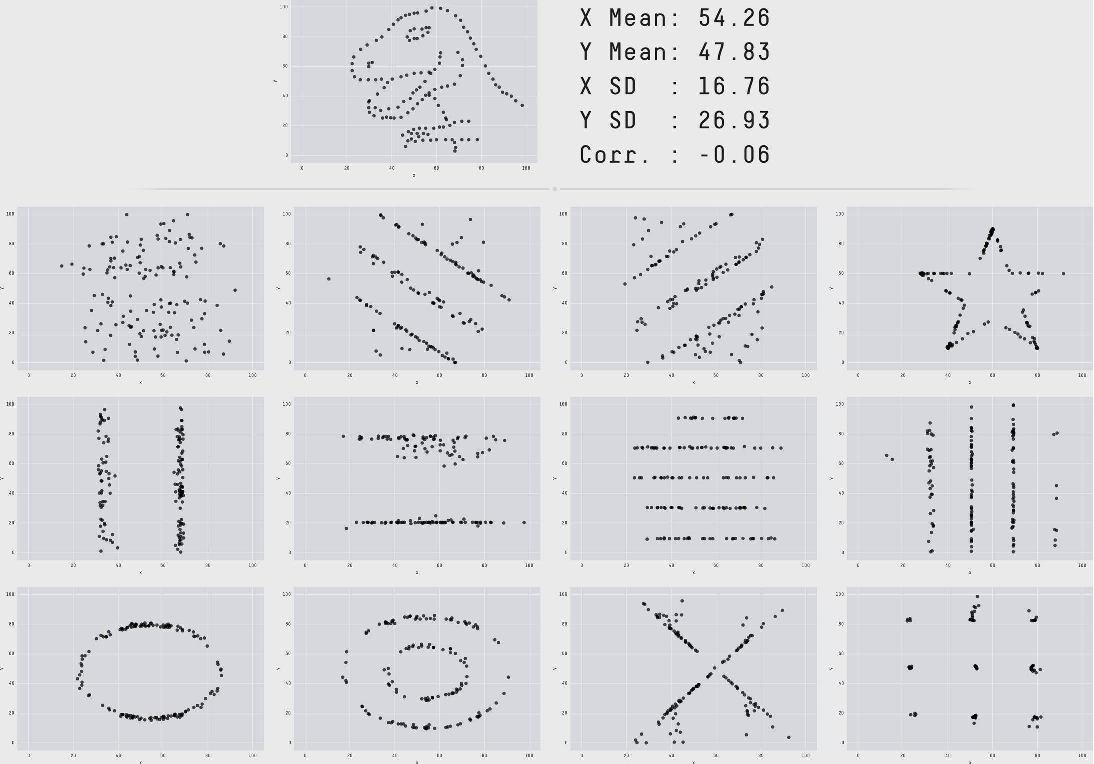
\includegraphics[width=0.92\linewidth]{figures/datasaurus_dozen.pdf}
\caption{The Datasaurus Dozen (Matejka \& Fitzmaurice, 2017)~\cite{matejka2017same}. All 13 distinct bivariate distributions share identical summary statistics up to two decimal places: horizontal mean $\bar{x} = 54.26$, vertical mean $\bar{y} = 47.83$, standard deviations $s_x = 16.76, s_y = 26.93$, and Pearson correlation coefficient $r = -0.06$. Yet their true empirical geometries range from a Tyrannosaurus Rex to concentric rings, starbursts, and parallel lines.}
\label{fig:slide_datasaurus}
\end{figure}

Figure~\ref{fig:slide_datasaurus} illustrates the \textbf{Datasaurus Dozen} experiment~\cite{matejka2017same}, an eloquent modern generalization of Anscombe's 1973 quartet. Each of the 13 bivariate datasets consists of 142 points and exhibits identical numerical properties to two decimal places:
\begin{equation}
\bar{x} = 54.26, \quad \bar{y} = 47.83, \quad s_x = 16.76, \quad s_y = 26.93, \quad r_{xy} = -0.06.
\label{eq:datasaurus_stats}
\end{equation}
An algorithm or practitioner relying solely on these metrics would conclude that all 13 datasets represent identical physical mechanisms. Yet inspecting the geometric plots reveals entirely distinct realities: one is a dinosaur, another is a high-density cluster surrounded by an outer ring, and another is a sequence of discrete vertical stripes.

To understand mathematically why summary statistics fail so catastrophically, consider the analytical formula for the \textbf{sample Pearson correlation coefficient} $r_{xy}$:
\begin{equation}
r_{xy} = \frac{\sum_{i=1}^N (x_i - \bar{x})(y_i - \bar{y})}{\sqrt{\sum_{i=1}^N (x_i - \bar{x})^2} \sqrt{\sum_{i=1}^N (y_i - \bar{y})^2}}.
\label{eq:pearson_correlation_formula}
\end{equation}
Equation~\eqref{eq:pearson_correlation_formula} measures exclusively \textbf{first-order linear co-variation}. When the underlying structural relationship is non-linear (such as a circle $x^2 + y^2 = R^2$, a parabola $y = x^2$, or a complex contour), deviations above and below the mean cancel out symmetrically in the numerator $\sum (x_i - \bar{x})(y_i - \bar{y}) \approx 0$. 

Furthermore, summary statistics completely discard:
\begin{itemize}[noitemsep]
  \item High-order statistical moments: skewness ($\mathbb{E}[(X-\mu)^3]/\sigma^3$) and kurtosis ($\mathbb{E}[(X-\mu)^4]/\sigma^4$).
  \item Multi-modal cluster topology and manifold connectivity.
  \item Heavy-tailed extreme values and catastrophic outlier distributions.
\end{itemize}
Hence, the golden imperative of machine learning: \textbf{Never trust summary statistics alone; always visualize and deeply inspect the data before modeling.}

\subsection{Pillar 1: Observe the data (Exploratory visualization and feature spaces)}
\label{sec:pillar_1_observe}

The first rule of machine learning is to open the dataset directory and directly examine the individual instances. In tabular domains or low-dimensional problems ($d \le 3$), scatter plots, histograms, and pair-wise correlation grids allow immediate visual diagnosis.

However, modern deep learning typically operates on extremely high-dimensional spaces: an uncompressed $256 \times 256$ RGB image lives in $\mathbb{R}^{196,608}$, and feature embeddings extracted from foundation models live in $\mathbb{R}^{1,024}$ or $\mathbb{R}^{4,096}$. Humans cannot directly visualize geometries beyond three dimensions. To observe such data, practitioners deploy mathematical projection and dimensionality reduction techniques:
\begin{itemize}[noitemsep]
  \item \textbf{Principal Component Analysis (PCA)}: Identifies the orthogonal directions of maximal variance by computing the eigenvectors of the empirical covariance matrix $\mathbf{\Sigma} = \frac{1}{N}\mathbf{X}^\top \mathbf{X}$, projecting $d$-dimensional representations onto the leading 2D or 3D principal sub-space.
  \item \textbf{Non-linear Manifold Learning}: Methods such as $t$-Distributed Stochastic Neighbor Embedding ($t$-SNE) and Uniform Manifold Approximation and Projection (UMAP) preserve local neighborhood topologies, unrolling complex non-linear manifolds into interpretable 2D diagnostic visual maps.
\end{itemize}

\paragraph{Critical oral exam insight: Knowing your dataset.}
In the oral examination, a fundamental line of questioning focuses on dataset mastery: \emph{Which benchmark did you use in your project or paper analysis? What semantic object categories does it contain? How many total instances are present, and what is the exact sample distribution across classes?} A candidate who views data as an interchangeable numeric matrix without knowing its class taxonomy, sensor resolution, or subgroup composition demonstrates a shallow understanding. A true machine learner understands the physical reality generating each feature coordinate.

\subsection{Pillar 2: Summarize uncertainty (Distributions and probabilistic frameworks)}
\label{sec:pillar_2_uncertainty}

Rather than condensing a feature coordinate into a single scalar average $\bar{x}$, rigorous data analysis models uncertainty through full probability distributions:
\begin{equation}
p(\mathbf{x}) \quad \text{or} \quad p(\mathbf{x} \mid y).
\end{equation}
As derived in Section~\ref{sec:data_uncertainty}, uncertainty comprises both irreducible sensor stochasticity (aleatoric) and epistemic parameter ignorance arising from data sparsity. In safety-critical applications—such as autonomous navigation or medical oncology—a point prediction $\hat{y} = f(\mathbf{x})$ without an accompanying confidence interval or posterior distribution $p(y \mid \mathbf{x})$ is dangerous. Modeling the full distribution provides the foundational calculus for Bayes decision theory, hypothesis testing, and risk-aware decision boundaries.

\subsection{Pillar 3: Search for constraints and invariances (Prior knowledge)}
\label{sec:pillar_3_prior_knowledge}

Without prior knowledge, an algorithm facing a finite dataset $\mathcal{D}_N$ must search through the uncountably infinite universe of mathematical functions that interpolate the points. Prior domain knowledge acts as a powerful mathematical filter, restricting the hypothesis space $\mathcal{H}$ to functions that obey known physical laws, geometric symmetries, and environmental constraints.

\paragraph{Historical case study: Alan Turing and the Enigma machine.}
The power of prior constraints to collapse search complexity is historically illustrated by Alan Turing's codebreaking triumph at Bletchley Park during World War II (dramatized in \emph{The Imitation Game}). The German military Enigma cipher machine possessed an astronomical keyspace: with multiple rotating rotors, ring settings, and a plugboard (\emph{Steckerbrett}), the machine offered approximately $1.5 \times 10^{20}$ possible daily wiring configurations. A brute-force search over this space was physically impossible, even with electromechanical computing machines (the \emph{Bombes}), within the daily 24-hour window before settings changed.

Turing's decisive insight was discovering an empirical invariance—a deterministic constraint in the communication protocol. German telegraph operators routinely began their first daily transmissions at exactly 06:00 with standardized meteorological reports containing invariant phrasing:
\begin{equation}
\text{\emph{Wetterbericht}} \quad (\text{"Weather Report"}),
\end{equation}
and frequently concluded messages with the obligatory military salutation:
\begin{equation}
\text{\emph{Heil Hitler}}.
\end{equation}
These predictable, recurring plaintext sequences (known as \textbf{cribs}) provided deterministic anchors between known plaintext and observed ciphertext. By enforcing these known linguistic constraints, Turing's Bombe did not have to search the entire combinatorial space of billions of permutations; the search space collapsed to a tiny feasible subset that the machines could eliminate in minutes.

\paragraph{Machine learning formulation.}
In statistical machine learning, prior knowledge functions in precisely the same manner: it dramatically reduces the volume of the hypothesis space $|\mathcal{H}|$ that must be searched during optimization. 
\begin{itemize}[noitemsep]
  \item If domain physics indicates that a signal originates from a continuous periodic industrial process (e.g., turbine vibration or seasonal temperature oscillation), searching over arbitrary high-degree polynomials is wasteful and leads to catastrophic boundary oscillations. Instead, the practitioner restricts $\mathcal{H}$ to a sinusoidal basis family:
  \begin{equation}
  f(x; \mathbf{w}) = A \sin(\omega x + \phi) + b.
  \end{equation}
  \item In computer vision, our prior knowledge that physical objects retain their semantic identity regardless of where they appear in the visual field directly justifies imposing \textbf{translation equivariance} via Convolutional Neural Networks ($f(T_g(\mathbf{x})) = T_g(f(\mathbf{x}))$), eliminating billions of redundant parameters compared to unconstrained fully connected layers.
\end{itemize}
Prior knowledge is the most effective regularizer: it saves optimization time, prevents overfitting, and minimizes the sample complexity required to achieve high generalization.

\subsection{Pillar 4: Find a model to explain the data (Families, capacity, and coordinate linearization)}
\label{sec:pillar_4_model_family}

Once data has been observed and prior constraints identified, the machine learner selects an appropriate mathematical model family $f(\mathbf{x}; \boldsymbol{\theta})$ to explain the relationship between input $\mathbf{x}$ and target $y$.

\paragraph{Model family complexity trade-offs.}
Consider fitting a two-dimensional dataset $\{(x_i, y_i)\}_{i=1}^N$:
\begin{itemize}[noitemsep]
  \item \textbf{Degree 1 Polynomial (Linear)}: $y = w_1 x + w_0$. Imposes high inductive bias; requires fitting only 2 scalar parameters. Fast to optimize, but suffers from underfitting if the true physical relationship exhibits curvature.
  \item \textbf{Degree 2 Polynomial (Quadratic)}: $y = w_2 x^2 + w_1 x + w_0$. Requires fitting 3 parameters; models parabolic trajectories.
  \item \textbf{Degree 3 Polynomial (Cubic)}: $y = w_3 x^3 + w_2 x^2 + w_1 x + w_0$. Requires fitting 4 parameters; captures inflection points.
  \item \textbf{Parametric 2D Curves}: Expressing coordinates parametrically as $(x(t), y(t)) = (a_x t + b_x, a_y t + b_y)$ introduces 4 parameters. While more flexible for trajectories, it doubles optimization requirements relative to a standard Cartesian linear model.
\end{itemize}

\paragraph{Coordinate transformations and the power of linearization.}
An expert machine learner does not merely increase model capacity when faced with geometrically complex data; they look for coordinate transformations that simplify the problem.

Consider a dataset whose points form an Archimedean spiral or circular ring centered at $(x_c, y_c)$. In standard Cartesian coordinates $(x, y)$, describing this trajectory with an explicit algebraic function $y = f(x)$ is impossible because the curve fails the vertical line test (a single $x$ maps to multiple values of $y$). Attempting to fit a high-degree Cartesian polynomial results in severe optimization instabilities.

Instead of adopting an unwieldy high-capacity black box, the practitioner shifts the origin to the empirical data centroid $(x_c, y_c)$ and transforms the coordinates into polar space:
\begin{equation}
r = \sqrt{(x - x_c)^2 + (y - y_c)^2}, \quad \theta = \operatorname{atan2}(y - y_c, x - x_c).
\label{eq:polar_transformation}
\end{equation}
In polar coordinates $(r, \theta)$, the complex spiral trajectory unrolls into an elementary linear relationship:
\begin{equation}
r(\theta) = a \theta.
\label{eq:linear_polar_spiral}
\end{equation}
By simply changing the geometric frame of reference, the learning problem reduces from fitting an intractable non-linear model to fitting a \textbf{single linear parameter} $a$! Mathematical sophistication in representation simplifies computational optimization.

\subsection{Pillar 5: Represent the data (Handcrafted features vs. geometric dimensionality)}
\label{sec:pillar_5_representation}

Learning algorithms do not ingest raw physical reality; they process mathematical representations. In classical machine learning (from the 1980s through 2010), representations were constructed via manual feature engineering guided by human domain experts.

\paragraph{The Fisher Iris paradigm.}
Consider the classical problem of classifying botanical species of Iris flowers into \emph{Iris setosa} and \emph{Iris versicolor}. Feeding raw, unprocessed botanical descriptions to a classifier yields poor results. Instead, a human botanical expert identifies the two morphological measurements that carry discriminative power:
\begin{equation}
x_1 = \text{Petal Length}, \quad x_2 = \text{Sepal Length}.
\end{equation}
Projecting each flower instance into this engineered 2D feature space $\mathbf{x} = [x_1, x_2]^\top \in \mathbb{R}^2$ separates the two species cleanly, allowing a simple Support Vector Machine (SVM) or linear hyperplane to achieve near-perfect classification.

\paragraph{Resolving non-separable distributions: Two foundational strategies.}
When classes overlap in a chosen feature space and cannot be separated linearly, the machine learner faces two distinct design choices:
\begin{enumerate}
  \item \textbf{Invest in Classifier Complexity}: Retain the current low-dimensional feature space, but replace the linear classifier with an intricate, highly non-linear decision boundary (e.g., high-degree polynomial kernels, deep decision trees, or multi-layer neural networks).
  \item \textbf{Invest in Representation (Lifting the Dimension)}: Consult domain experts or extract additional feature measurements (e.g., adding $x_3 = \text{Petal Width}$ and $x_4 = \text{Sepal Width}$). By embedding the data into a higher-dimensional space $\mathbb{R}^d$ ($d > 2$), entangled clusters disentangle naturally, allowing an elementary linear classifier to separate them with high margin.
\end{enumerate}

\paragraph{Dimensionality reduction and manifold unrolling.}
Conversely, when raw data is unnecessarily high-dimensional (e.g., 100 sensor readings that are heavily correlated), the data may lie on a low-dimensional intrinsic manifold (e.g., a 2D sheet embedded in $\mathbb{R}^3$). In such cases, applying linear PCA or non-linear manifold unrolling reduces dimensionality, eliminates multicollinearity, suppresses measurement noise, and circumvents the curse of dimensionality.

\subsection{Pillar 6: Joint end-to-end learning via computing power (The playing cards analogy)}
\label{sec:pillar_6_joint_learning}

The decisive paradigm shift of the 2010 Deep Learning revolution was abandoning decoupled manual feature engineering in favor of \textbf{end-to-end joint representation learning}.

\begin{figure}[htbp]
\centering
\begin{tikzpicture}[>=Stealth, node distance=1.2cm, scale=0.95, every node/.style={transform shape}]
  % Styles
  \tikzset{
    card/.style = {draw=politoNavy, fill=white, rounded corners=4pt, minimum width=1.2cm, minimum height=1.65cm, line width=1.1pt, font=\bfseries},
    taskbox/.style = {draw=deepdiveTeal, fill=white, rounded corners=5pt, line width=1.1pt, inner sep=6pt, font=\small, align=left}
  }

  % Raw Playing Cards Deck
  \node[font=\bfseries\normalsize, text=politoNavy] (title) at (0, 3.2) {Raw Observation: Standard 52-Card Deck $\mathbf{x} \in \mathcal{X}$};

  % Visual Cards
  \node[card] (c1) at (-2.2, 1.8) {$\spadesuit$\,\text{Q}};
  \node[card, draw=examred, text=examred] (c2) at (-0.75, 1.8) {$\heartsuit$\,\text{A}};
  \node[card] (c3) at (0.75, 1.8) {$\clubsuit$\,\text{K}};
  \node[card, draw=examred, text=examred] (c4) at (2.2, 1.8) {$\diamondsuit$\,10};

  % Intrinsic Features Panel
  \node[draw=gray!60, fill=gray!8, rounded corners=4pt, inner sep=5pt, font=\scriptsize, align=center] (feat) at (0, 0.4) {
    \textbf{Generic Intrinsic Attributes:}\\
    $\text{Rank} \in \{\text{A}, 2, \dots, \text{K}\}, \quad \text{Suit} \in \{\spadesuit, \heartsuit, \clubsuit, \diamondsuit\}, \quad \text{Color} \in \{\text{Black}, \text{Red}\}$
  };

  % Downstream Task Nodes
  \node[taskbox, draw=politoNavy] (t1) at (-4.2, -1.8) {
    \textbf{Task 1: Poker}\\
    \rule{3.2cm}{0.4pt}\\
    $\bullet$ \textbf{Rank}: Crucial (straights, pairs)\\
    $\bullet$ \textbf{Suit}: Crucial (flushes)\\
    $\bullet$ \textbf{Color}: \textit{Redundant / Irrelevant}
  };

  \node[taskbox, draw=intuitiongreen] (t2) at (0, -1.8) {
    \textbf{Task 2: Blackjack}\\
    \rule{3.2cm}{0.4pt}\\
    $\bullet$ \textbf{Rank}: Additive value only\\
    $\bullet$ \textbf{Suit}: \textit{Completely irrelevant}\\
    $\bullet$ \textbf{Color}: \textit{Completely irrelevant}
  };

  \node[taskbox, draw=examred] (t3) at (4.2, -1.8) {
    \textbf{Task 3: Hearts}\\
    \rule{3.2cm}{0.4pt}\\
    $\bullet$ \textbf{Rank \& Suit Jointly}:\\
    \quad $\spadesuit\,\text{Q} \implies -13$ penalty pts!\\
    \quad $\heartsuit \implies -1$ pt each\\
    $\bullet$ \textbf{Color}: \textit{No independent role}
  };

  % Connecting Arrows
  \draw[->, very thick, politoNavy] (feat.south) -- ++(0, -0.3) -| (t1.north) 
    node[pos=0.25, above, font=\scriptsize\bfseries, text=politoNavy] {Task Mapping $\phi_{\text{poker}}(\mathbf{x})$};
  \draw[->, very thick, intuitiongreen] (feat.south) -- (t2.north)
    node[pos=0.45, right, font=\scriptsize\bfseries, text=intuitiongreen] {$\phi_{\text{blackjack}}(\mathbf{x})$};
  \draw[->, very thick, examred] (feat.south) -- ++(0, -0.3) -| (t3.north)
    node[pos=0.25, above, font=\scriptsize\bfseries, text=examred] {$\phi_{\text{hearts}}(\mathbf{x})$};

  % Core Moral Callout
  \node[draw=politoNavy, fill=politoNavy!5, rounded corners=5pt, line width=1.2pt, font=\small, align=center, inner sep=6pt] at (0, -3.8) {
    \textbf{The Representation Principle:} There is no such thing as an optimal ``universal'' feature set in a vacuum.\\
    Feature utility $\phi(\mathbf{x})$ is \textbf{strictly conditioned} on the target task $\mathcal{T}$ and objective loss $\mathcal{L}(\hat{y}, y)$.
  };
\end{tikzpicture}
\caption{The playing card representation analogy: context-dependent, task-driven features. In a standard 52-card deck, cards possess invariant intrinsic properties (rank, suit, and color). However, the utility of these features depends entirely on the game being played: in Hearts, the Queen of Spades carries devastating negative penalty points; in Poker, flushes require tracking suits while rank determines straights; in Blackjack, suits and colors are completely irrelevant and only numeric card values matter.}
\label{fig:slide_card_representation}
\end{figure}

\paragraph{The playing cards analogy: Features are strictly task-driven.}
Why must representation learning be coupled directly to the learning task? The answer is illustrated by the card-game analogy depicted in Figure~\ref{fig:slide_card_representation}. 

A standard deck of playing cards contains 52 elements, each possessing fixed intrinsic attributes:
\begin{equation}
\text{Rank} \in \{\text{Ace}, 2, \dots, \text{King}\}, \quad \text{Suit} \in \{\heartsuit, \diamondsuit, \clubsuit, \spadesuit\}, \quad \text{Color} \in \{\text{Red}, \text{Black}\}.
\end{equation}
If you ask an expert to build a "universal feature representation" for a playing card, they cannot answer without knowing the game to be played:
\begin{itemize}[noitemsep]
  \item In \textbf{Poker}, suit is vital for detecting flushes, and rank order is vital for straights, whereas color is redundant.
  \item In \textbf{Blackjack}, suit and color are completely irrelevant; only the additive numeric value of the rank matters.
  \item In \textbf{Hearts}, the Queen of Spades ($\text{Q}\spadesuit$) carries a severe 13-point penalty, making that specific combination of suit and rank uniquely critical, while diamond cards carry zero penalty.
\end{itemize}
This pedagogical example reveals a core axiom of modern machine learning: \textbf{There is no universally optimal feature representation; features only make sense relative to the specific task $\mathcal{T}$ being solved!}

\paragraph{Shallow vs. Deep learning architectures.}
This principle explains why shallow machine learning frequently hit performance ceilings:
\begin{equation}
\text{Raw Data } \mathbf{x} \xrightarrow[\text{Human Expert}]{\text{Fixed Handcrafted Features}} \boldsymbol{\phi}(\mathbf{x}) \xrightarrow[\text{Learned}]{\text{Shallow Model}} \hat{y}.
\end{equation}
In shallow ML, the feature extractor $\boldsymbol{\phi}(\mathbf{x})$ is fixed and decoupled from the classifier. If the human expert's handcrafted descriptors omit subtle correlations essential for the downstream task, the classifier can never recover them.

In contrast, Deep Learning unifies representation extraction and task optimization into a single differentiable pipeline:
\begin{equation}
\text{Raw Data } \mathbf{x} \xrightarrow[\text{Differentiable Layers}]{\mathbf{W}_1, \mathbf{W}_2, \dots, \mathbf{W}_{L-1}} \mathbf{h}_{L-1}(\mathbf{x}) \xrightarrow[\text{Classification Head}]{\mathbf{W}_L} \hat{y}.
\end{equation}
Driven by the backpropagation of the task-specific loss gradient $\nabla_{\mathbf{W}} \ell(\hat{y}, y)$, the internal layers dynamically mold their intermediate representations $\mathbf{h}_l$ specifically to solve task $\mathcal{T}$.

\paragraph{ImageNet and hierarchical feature emergence.}
In the seminal 2012 AlexNet architecture trained on the 1,000-class ImageNet benchmark, inspecting the learned convolutional filter weights revealed a structured hierarchy of representation:
\begin{itemize}[noitemsep]
  \item \textbf{Early Layers (Layers 1--2)}: Extract generic low-level visual primitives: oriented Gabor-like edge filters across multiple angles, spatial frequency bars, and localized color blobs.
  \item \textbf{Intermediate Layers (Layers 3--4)}: Group low-level edges into composite textures, corners, repetitive grids, and structural object parts (e.g., circular wheel rims, mesh grilles, and animal eyes).
  \item \textbf{Deep Layers (Layer 5 and fully connected heads)}: Assemble object parts into holistic class-specific semantic representations (e.g., complete dog faces, bird beaks, and bicycle frames).
\end{itemize}
This hierarchical decomposition was not programmed by humans; it emerged autonomously from raw pixels driven entirely by gradient optimization on the cross-entropy task loss.

\subsection{Pillar 7: Avoid data bias, spurious correlations, and enforce fairness}
\label{sec:pillar_7_avoid_bias}

The final pillar governs the ethical and epistemological reliability of deployed models. A pervasive myth in society is that mathematical algorithms are inherently objective and immune to human prejudice. 

In reality, \textbf{machine learning models are objective only in the sense that they faithfully optimize their loss function on whatever empirical data they are fed.} If the training data contains historical societal inequities, unrepresentative demographic sampling, or spurious statistical artifacts, the model will not correct them; it will exploit them as optimal predictive shortcuts.

---

\section{Societal consequences of bias and the algorithmic frontier}
\label{sec:societal_bias_and_fairness}

When machine learning systems are deployed in real-world institutions—such as criminal justice, credit scoring, medical triage, and hiring—data bias ceases to be a theoretical optimization nuisance and becomes an active source of systemic harm.

\subsection{Spurious correlations as algorithmic shortcuts: The doctor vs. nurse dilemma}
\label{sec:spurious_shortcuts}

Machine learning models optimize purely for accuracy under their training distribution. When presented with training datasets that reflect historical gender imbalances in professional occupations, computer vision models learn to rely on spurious demographic shortcuts rather than true semantic features.

In benchmark experiments on occupation classification from photographs:
\begin{itemize}[noitemsep]
  \item A human expect the classifier to distinguish a doctor from a nurse by examining functional attire: stethoscopes, surgical masks, white laboratory coats, or specialized instruments.
  \item Instead, feature attribution maps (such as Grad-CAM) revealed that the deep networks were focusing directly on the subject's face to classify \textbf{gender}: if the subject was male, the network predicted "Doctor"; if the subject was female, it predicted "Nurse".
\end{itemize}
Because the scraped web training data had a high proportion of male doctors and female nurses, the model discovered that facial gender recognition was an easy statistical shortcut to achieve high training accuracy with minimal gradient effort. 

When deployed in clinical environments where female doctors and male nurses are present, the model failed catastrophically. This failure illustrates the fundamental machine learning adage: \textbf{"Garbage in, garbage out"}—if an algorithm is trained on biased data, it produces biased, untrustworthy predictions.

\subsection{The COMPAS recidivism case study and mathematical fairness}
\label{sec:compas_case_study}

The most consequential and widely analyzed real-world failure of algorithmic decision-making occurred in the United States criminal justice system with the \textbf{COMPAS} (Correctional Offender Management Profiling for Alternative Sanctions) algorithm, developed by Northpointe (now Equivant)~\cite{angwin2016machine}.

\paragraph{Algorithmic deployment in pretrial detention.}
COMPAS is a commercial risk-assessment instrument used by judges in multiple US jurisdictions to predict a criminal defendant's likelihood of reoffending (recidivism) within two years. The algorithm outputs a decile risk score from 1 (lowest risk) to 10 (highest risk). Judges routinely consult this scalar score when deciding whether a defendant should be granted pretrial release on bail or remanded to prison pending trial.

COMPAS was trained on historical criminal records and arrest histories spanning decades—a historical record heavily shaped by racially disparate policing practices, stop-and-frisk policies, and socio-economic profiling.

\paragraph{The 2016 ProPublica investigative audit.}
In a landmark 2016 investigative analysis, journalists Julia Angwin, Jeff Larson, Surya Mattu, and Lauren Kirchner from \emph{ProPublica} audited the COMPAS risk scores and subsequent two-year arrest records of over 7,000 individuals arrested in Broward County, Florida~\cite{angwin2016machine}. 

While the algorithm did not explicitly receive race as an input feature coordinate, it took 137 questionnaire responses and historical arrest counts that served as close proxies for socio-economic background and race. When ProPublica evaluated the accuracy of COMPAS across demographic groups, they discovered a severe, systematic racial asymmetry in prediction errors:
\begin{itemize}
  \item \textbf{Disparate False Positive Rate (FPR)}: Among defendants who \textbf{did not reoffend} during the subsequent two-year follow-up window, Black defendants were mistakenly classified as medium or high risk at almost \textbf{twice the rate} of White non-reoffenders:
  \begin{equation}
  \text{FPR}_{\text{Black}} = 44.9\% \quad \text{vs.} \quad \text{FPR}_{\text{White}} = 23.5\%.
  \label{eq:compas_fpr}
  \end{equation}
  \item \textbf{Disparate False Negative Rate (FNR)}: Conversely, among defendants who \textbf{did reoffend} within two years, White defendants were mistakenly classified as low risk at almost \textbf{twice the rate} of Black reoffenders:
  \begin{equation}
  \text{FNR}_{\text{White}} = 47.7\% \quad \text{vs.} \quad \text{FNR}_{\text{Black}} = 28.0\%.
  \label{eq:compas_fnr}
  \end{equation}
\end{itemize}
In human terms, the algorithm exhibited a severe asymmetric bias: it systematically projected future criminality onto innocent Black individuals while extending undue leniency and benefit of the doubt to White individuals who subsequently committed crimes.

\paragraph{The Impossibility Theorem of Algorithmic Fairness.}
The COMPAS controversy sparked an intense mathematical debate between Northpointe and academic computer scientists. Northpointe defended the tool by proving that COMPAS satisfied \textbf{Predictive Parity (Calibration within Groups)}: for any given risk score $s$ (e.g., score $= 7$), the probability that a defendant reoffends is roughly equal regardless of race:
\begin{equation}
P(Y = 1 \mid S = s, A = \text{Black}) \approx P(Y = 1 \mid S = s, A = \text{White}).
\label{eq:predictive_parity}
\end{equation}
ProPublica, by contrast, evaluated the algorithm according to \textbf{Error Rate Parity (Equalized Odds / Separation)}: requiring equal false positive rates and false negative rates across groups:
\begin{equation}
P(\hat{Y} = 1 \mid Y = 0, A = \text{Black}) \stackrel{?}{=} P(\hat{Y} = 1 \mid Y = 0, A = \text{White}).
\label{eq:error_rate_parity}
\end{equation}

In 2016, computer scientists Jon Kleinberg, Sendhil Mullainathan, and Manish Raghavan~\cite{kleinberg2016inherent} (and independently Alexandra Chouldechova) proved a foundational mathematical theorem known as the \textbf{Impossibility Theorem of Fairness}:

\begin{theorem}[Fairness Impossibility Theorem~\cite{kleinberg2016inherent}]
Let $Y \in \{0, 1\}$ be the true binary outcome, $\hat{Y} \in \{0, 1\}$ be the binary decision, and $A \in \{a, b\}$ be a sensitive demographic attribute. Suppose the base rates of the two groups are unequal:
\begin{equation}
P(Y = 1 \mid A = a) \ne P(Y = 1 \mid A = b),
\end{equation}
and the classifier is not a perfect predictor (i.e., its error rate is non-zero). Then, it is \textbf{mathematically impossible} for any algorithm to simultaneously satisfy:
\begin{enumerate}[noitemsep]
  \item \textbf{Calibration (Predictive Parity)}: $P(Y = 1 \mid \hat{Y} = 1, A = a) = P(Y = 1 \mid \hat{Y} = 1, A = b)$.
  \item \textbf{Equal False Positive Rates}: $P(\hat{Y} = 1 \mid Y = 0, A = a) = P(\hat{Y} = 1 \mid Y = 0, A = b)$.
  \item \textbf{Equal False Negative Rates}: $P(\hat{Y} = 0 \mid Y = 1, A = a) = P(\hat{Y} = 0 \mid Y = 1, A = b)$.
\end{enumerate}
\end{theorem}
Because historical arrest base rates differed between demographic groups due to structural socio-economic inequalities, satisfying calibration mathematically forced COMPAS to produce asymmetric false positive rates! 

This mathematical reality underscores why algorithmic fairness cannot be resolved purely by code: practitioners must consciously choose which fairness definition to prioritize based on legal, ethical, and societal values.

\subsection{Legal and regulatory safeguards: The EU AI Act (August 2024)}
\label{sec:eu_ai_act}

In response to scandals such as COMPAS and predatory biometric profiling, governments have instituted binding legal regulations. In \textbf{August 2024}, the European Union enacted into law the \textbf{Artificial Intelligence Act (EU AI Act)}, establishing the world's first comprehensive horizontal legal framework for AI governance.

The EU AI Act establishes a four-tiered risk-based regulatory pyramid:
\begin{enumerate}
  \item \textbf{Unacceptable Risk (Prohibited)}: AI systems that pose an intolerable threat to human safety and fundamental rights are banned outright. This includes government social credit scoring, cognitive behavioral manipulation targeting vulnerable populations, biometric categorization based on political/philosophical beliefs, and real-time biometric identification in public spaces by law enforcement (with narrow judicial exceptions).
  \item \textbf{High-Risk (Strictly Regulated)}: Systems deployed in critical sectors that directly impact human livelihoods, health, safety, and civil rights. Crucially, the EU AI Act classifies AI used in \textbf{the administration of justice, law enforcement, judicial bail decisions, credit scoring, employment recruitment, education grading, and critical infrastructure} as \textbf{High-Risk}.
  \item \textbf{General Purpose AI (GPAI)}: Large foundation models (e.g., frontier LLMs) must comply with transparency mandates, copyright documentation, and systemic risk assessments for frontier capabilities exceeding $10^{25}$ FLOPs.
  \item \textbf{Minimal / Low Risk}: Systems like spam filters, AI recommendation engines, or video games, which remain largely unconstrained.
\end{enumerate}

\paragraph{Mandatory compliance for High-Risk AI.}
Under the EU AI Act, systems operating in the justice and law enforcement domains (such as COMPAS-like recidivism tools) face stringent legal obligations before they can enter the EU market:
\begin{itemize}[noitemsep]
  \item \textbf{Mandatory Data Governance}: Training, validation, and testing datasets must be vetted for representative demographic balance, data quality, and statistical bias mitigation prior to training.
  \item \textbf{Mandatory Human Oversight}: AI models cannot automate judicial sentences or legal determinations autonomously. A qualified human magistrate must retain effective supervisory control (\emph{human-in-the-loop}), with full authority to override, reject, or ignore algorithmic outputs.
  \item \textbf{Traceability and Audit Logs}: High-risk systems must automatically log their operating states, input distributions, and decision paths to facilitate post-hoc judicial audits.
\end{itemize}
While the EU AI Act legally applies only within European jurisdiction, its extraterritorial scope binds any international entity or US provider deploying AI systems whose outputs affect individuals residing within the European Union.

\subsection{Domain shift, Sim-to-Real gap, and the limits of i.i.d. generalization}
\label{sec:domain_shift_and_sim2real}

Statistical learning theory rests entirely on the foundational assumption that training samples and future deployment test samples are drawn \textbf{independently and identically distributed (i.i.d.)} from the exact same stationary probability distribution:
\begin{equation}
p_{\text{train}}(\mathbf{x}, y) \equiv p_{\text{test}}(\mathbf{x}, y) = p_{\text{data}}(\mathbf{x}, y).
\label{eq:iid_stationarity_assumption}
\end{equation}
In real-world deployment, this assumption is universally violated.

\begin{figure}[htbp]
\centering
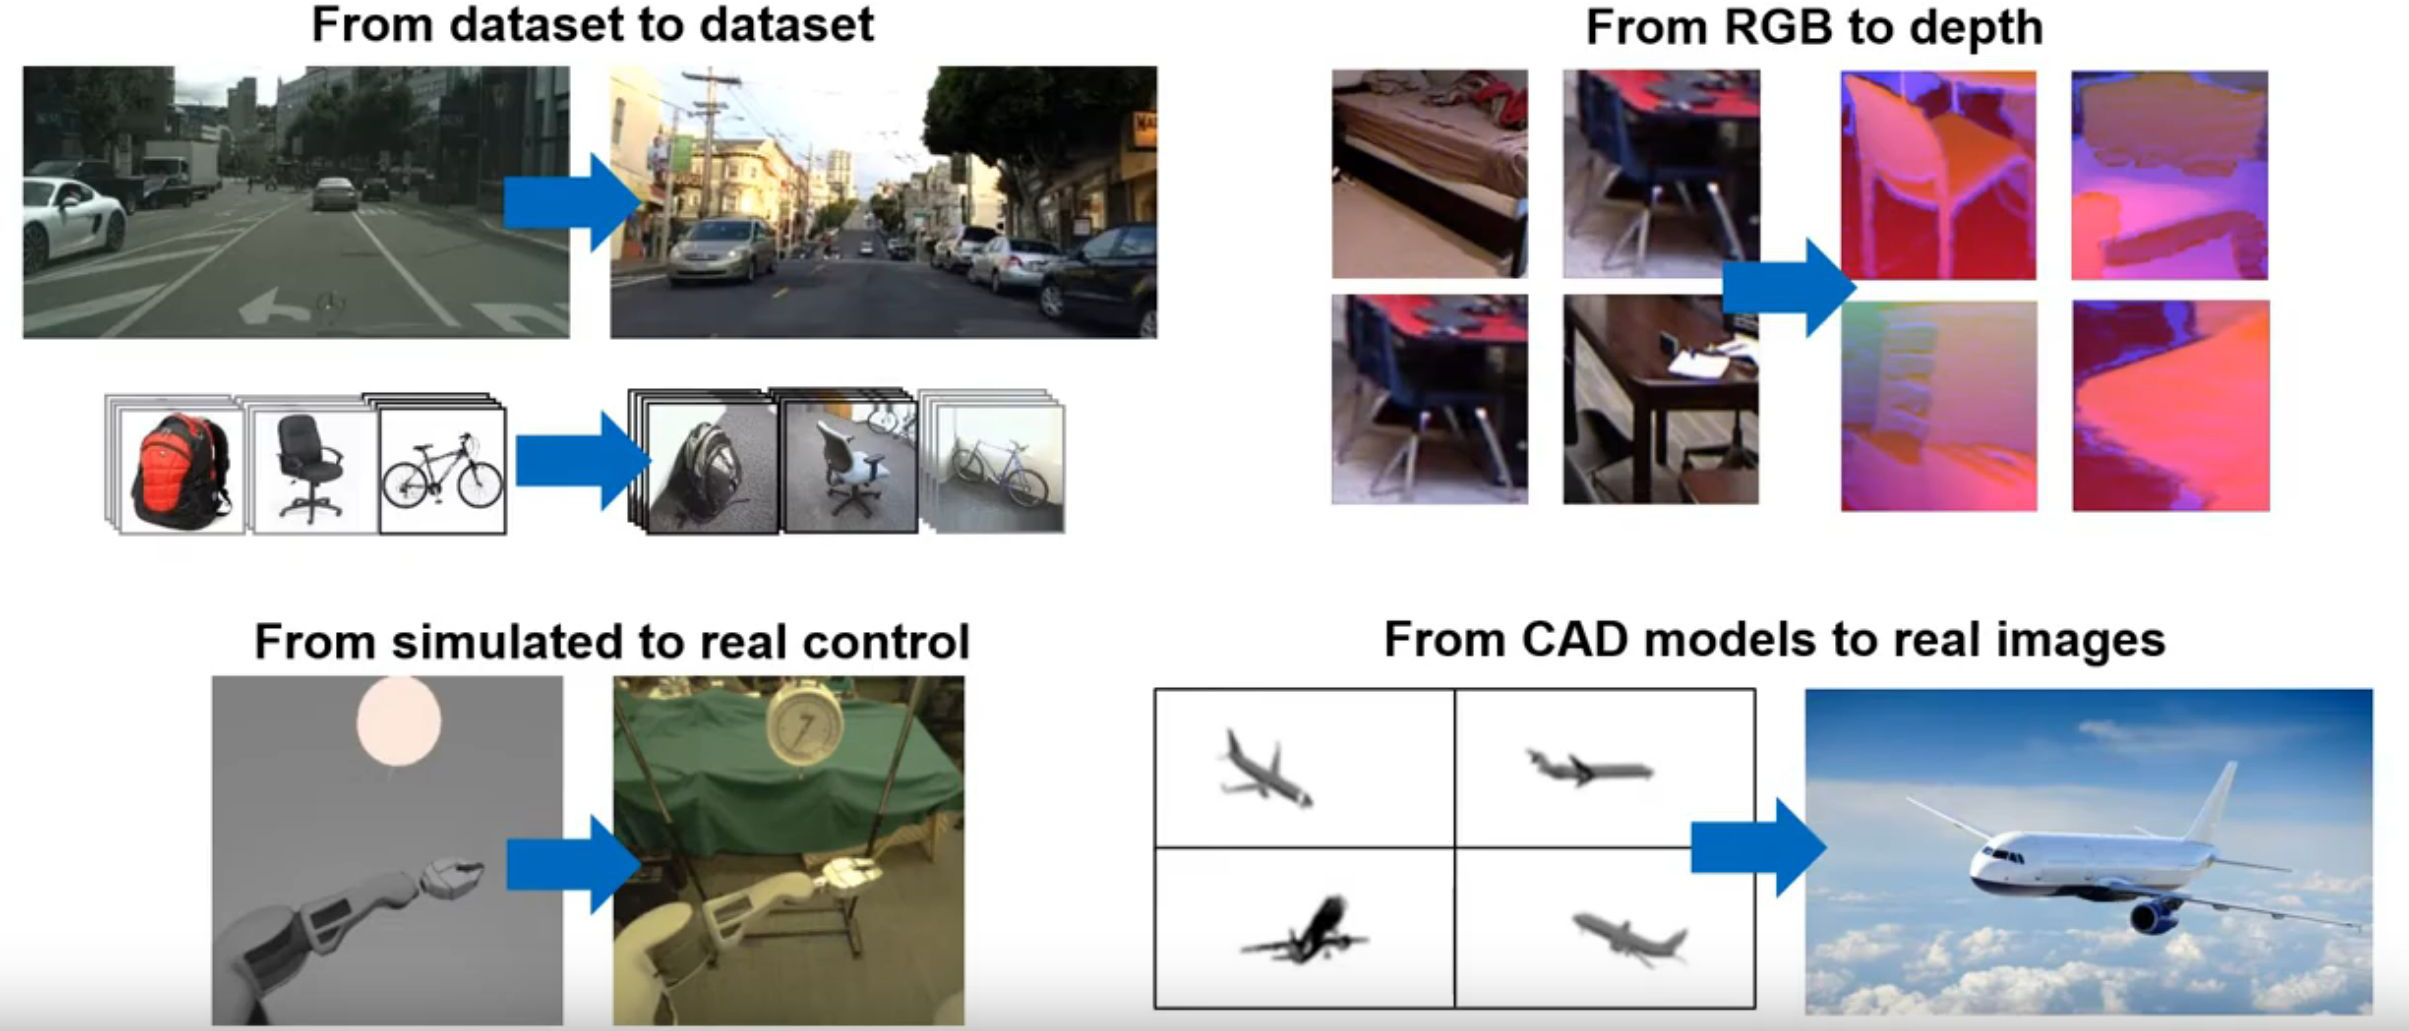
\includegraphics[width=0.92\linewidth]{figures/domain_shift_office31.png}
\caption{Dataset bias and domain shift (Torralba \& Efros, 2011; Saenko et al., 2010)~\cite{torralba2011unbiased,saenko2010adapting}. When an image classifier trained on high-quality product images (e.g., Amazon catalogue photos) is deployed on real-world webcam photos or mobile phone snapshots, accuracy drops precipitously due to distribution shift across lighting, background clutter, and camera angles.}
\label{fig:slide_dataset_bias}
\end{figure}

As shown in Figure~\ref{fig:slide_dataset_bias}, when models encounter \textbf{domain shift}, test accuracy drops precipitously. The two primary mathematical forms of domain shift are:
\begin{itemize}
  \item \textbf{Covariate Shift}: The marginal input feature distribution shifts ($p_{\text{train}}(\mathbf{x}) \ne p_{\text{test}}(\mathbf{x})$), while the posterior conditional label boundary remains invariant ($P(y \mid \mathbf{x})$ is constant).
  \item \textbf{Concept Drift}: The conditional label distribution itself changes ($P_{\text{train}}(y \mid \mathbf{x}) \ne P_{\text{test}}(y \mid \mathbf{x})$), meaning identical input observations map to different semantic classes over time.
\end{itemize}

\paragraph{Autonomous driving and the Sim-to-Real gap.}
A vivid empirical example occurs in autonomous robotics and self-driving vehicles:
\begin{itemize}
  \item \textbf{Geographic and Environmental Domain Shift}: An autonomous driving perception network trained exclusively on camera footage collected in sunny daylight conditions in Rome will fail catastrophically when deployed during a heavy snowstorm at night in Beijing. Lighting conditions, road textures, precipitation scatter, and pedestrian behaviors change drastically ($p_{\text{train}}(\mathbf{x}) \ne p_{\text{test}}(\mathbf{x})$).
  \item \textbf{The Sim-to-Real Gap}: Autonomous robots cannot be trained from scratch in physical reality because random exploration would cause physical collisions, vehicle crashes, and immense financial cost. Consequently, roboticists and autonomous vehicle developers train perception systems inside high-fidelity 3D synthetic simulators or game engines like \textbf{Grand Theft Auto V (GTA V)} and CARLA. 
\end{itemize}
While synthetic video game data is infinitely cheap, fully scalable, and comes with free, perfect pixel-level semantic segmentation annotations, real-world deployment reveals a severe \textbf{Sim-to-Real domain gap}. Synthetic graphics rendering engines lack the high-frequency physical noise, optical aberrations, dynamic specular reflections, and chaotic imperfections of the physical world. A model that achieves $99\%$ semantic segmentation accuracy inside GTA V drops precipitously when tested on physical highway cameras.

Overcoming this gap requires modern techniques beyond classical i.i.d. learning:
\begin{itemize}[noitemsep]
  \item \textbf{Unsupervised Domain Adaptation (UDA)}: Aligning source and target feature representations via adversarial minimax objectives (e.g., Domain-Adversarial Neural Networks, DANN~\cite{ganin2016domain}).
  \item \textbf{Domain Randomization}: Randomizing simulation lighting, camera angles, textures, and weather dynamics during synthetic training so that physical reality appears to the network as merely another synthetic variation.
  \item \textbf{Continual / Lifelong Learning}: Updating network parameters online in response to non-stationary environments without catastrophically forgetting previously mastered domains.
\end{itemize}
The study of dataset bias, domain adaptation, and statistical robustness represents the true frontier of modern machine learning, bridging laboratory benchmarks to robust physical reality.


\chapter{Probability Theory, Statistical Decision Theory, and Empirical Risk Minimization}
\label{sec:probability_and_decision_theory}

Machine learning is fundamentally the science of making principled inferences and optimal decisions under uncertainty. Every real-world sensor reading is perturbed by noise, every dataset represents an incomplete sample of reality, and every prediction about future test instances carries inherent ambiguity. To build algorithms that learn from data, we must ground our reasoning in the mathematical framework of \textbf{probability theory} and \textbf{statistical decision theory}.

In this chapter, we develop the foundations of probabilistic machine learning. We begin from the axiomatic formulation of probability spaces and Cox's plausibility postulates, progress through multivariable joint distributions and inference by enumeration, establish Bayes' theorem with an exact geometric probability area formulation, resolve probabilistic paradoxes such as the Monty Hall problem, and derive the Naïve Bayes classifier with Laplace smoothing. 

We then bridge probability to modern machine learning: formalizing task-dependent loss functions, True Risk, the Bayes Optimal Classifier, Empirical Risk Minimization (ERM), Probably Approximately Correct (PAC) generalization bounds, underfitting versus overfitting trade-offs, rigorous validation protocols ($k$-fold and Leave-One-Out cross-validation), regularization, and the complete closed-form calculus derivations of Ordinary Least Squares (Normal Equations) and Ridge Regression.

---

\section{Foundations of probability: Sample spaces, events, and plausibility axioms}
\label{sec:foundations_of_probability}

Why are basic statistics and probability indispensable for machine learning? As established in lecture, machine learning models do not possess omniscience; they process finite empirical observations to infer unobserved truths. Probability provides the formal mathematical calculus to:
\begin{itemize}[noitemsep]
  \item Quantify our degree of belief in competing hypotheses given partial, noisy evidence.
  \item Formulate principled classification rules that minimize expected misclassification costs.
  \item Bridge observed finite datasets to unobserved continuous population distributions.
\end{itemize}

\subsection{Sample spaces, events, and probability measures}
\label{sec:sample_spaces_and_events}

To formalize uncertainty mathematically, we construct a probability space as a measure-theoretic triplet $(\Omega, \mathcal{F}, P)$:
\begin{enumerate}
  \item \textbf{Sample Space} $\Omega$: The set of all conceivable, mutually exclusive outcomes of a physical or conceptual experiment:
  \begin{itemize}[noitemsep]
    \item \emph{Discrete Sample Spaces}: When outcomes can be enumerated. For a single coin flip, $\Omega = \{\text{Heads}, \text{Tails}\}$; for a 6-sided die, $\Omega = \{1, 2, 3, 4, 5, 6\}$; for a standard deck of cards, $|\Omega| = 52$.
    \item \emph{Continuous Sample Spaces}: When outcomes represent uncountably infinite measurements, such as sensor voltages, physical temperatures, or spatial coordinates: $\Omega = \mathbb{R}$ or $\Omega = \mathbb{R}^d$.
  \end{itemize}
  \item \textbf{Event} $A \subseteq \Omega$: An event is any subset of the sample space whose occurrence we wish to evaluate. For example, rolling an even number on a die corresponds to the event subset $A = \{2, 4, 6\} \subset \Omega$.
  \item \textbf{Probability Measure} $P(A)$: A real-valued function $P: \mathcal{F} \to [0, 1]$ that assigns a scalar plausibility to event $A$. Visually, if the entire sample space $\Omega$ is represented as a geometric region with unit area ($P(\Omega) = 1$), the probability of event $A$ is the fraction of total area covered by subset $A$.
\end{enumerate}

\subsection{The Kolmogorov probability axioms and set-theoretic consequences}
\label{sec:kolmogorov_axioms}

In 1933, Andrey Kolmogorov established that any valid mathematical calculus of probability must satisfy three non-negotiable axioms:
\begin{definition}[Kolmogorov Probability Axioms~\cite{bishop2024deep}]
Let $\Omega$ be a sample space and $\mathcal{F}$ be the collection of valid events. A function $P: \mathcal{F} \to [0, 1]$ is a probability measure if and only if:
\begin{enumerate}
  \item \textbf{Axiom 1 (Non-Negativity)}: For every event $A \subseteq \Omega$,
  \begin{equation}
  P(A) \ge 0.
  \label{eq:kolmogorov_nonnegativity}
  \end{equation}
  \item \textbf{Axiom 2 (Total Measure / Normalization)}: The probability of the entire sample space is unity:
  \begin{equation}
  P(\Omega) = 1.
  \label{eq:kolmogorov_normalization}
  \end{equation}
  \item \textbf{Axiom 3 (Countable Additivity / $\sigma$-Additivity)}: For any sequence of pairwise mutually exclusive events $\{A_1, A_2, \dots\}$ (where $A_i \cap A_j = \emptyset$ for all $i \ne j$):
  \begin{equation}
  P\left(\bigcup_{i=1}^\infty A_i\right) = \sum_{i=1}^\infty P(A_i).
  \label{eq:kolmogorov_additivity}
  \end{equation}
\end{enumerate}
\end{definition}

From these three minimal axioms, the foundational properties of probability calculus follow directly:
\begin{itemize}[noitemsep]
  \item \textbf{Empty Set}: $P(\emptyset) = 0$.
  \item \textbf{Complementation Rule}: Since $A \cup A^c = \Omega$ and $A \cap A^c = \emptyset$, Axioms 2 and 3 imply:
  \begin{equation}
  P(A^c) = 1 - P(A).
  \label{eq:complementation_rule}
  \end{equation}
  \item \textbf{Monotonicity}: If event $A$ is a subset of event $B$ ($A \subseteq B$), then $P(A) \le P(B)$.
  \item \textbf{Inclusion-Exclusion Principle}: For any two events $A$ and $B$ (not necessarily disjoint):
  \begin{equation}
  P(A \cup B) = P(A) + P(B) - P(A \cap B).
  \label{eq:inclusion_exclusion_rule}
  \end{equation}
\end{itemize}

\subsection{Cox's plausibility postulates: Why probability calculus is unique}
\label{sec:cox_postulates}

A profound foundational question in machine learning is: \emph{Why must we quantify uncertainty using Kolmogorov probability calculus rather than inventing arbitrary scoring heuristics, fuzzy logics, or ad-hoc confidence metrics?}

In 1946, physicist Richard Cox~\cite{cox1946probability,jaynes2003probability} proved that any mathematical framework for plausible reasoning that satisfies basic qualitative desiderata of human common sense is \textbf{isomorphic to standard probability theory}. Cox defined three commonsense postulates:
\begin{enumerate}
  \item \textbf{Real-Valued Representation}: Degrees of plausibility are represented by real scalar numbers: if hypothesis $A$ is more plausible than hypothesis $B$, and $B$ is more plausible than $C$, then $p(A) > p(B) > p(C)$.
  \item \textbf{Qualitative Correspondence}: As the plausibility of hypothesis $A$ increases given background information, the plausibility of its negation $\neg A$ must strictly decrease.
  \item \textbf{Consistency}: If a conclusion can be reasoned out in multiple mathematically valid ways, every equivalent line of reasoning must yield the identical numerical plausibility value.
\end{enumerate}
From these three qualitative postulates alone, Cox proved through functional equations that the product rule $P(A \cap B) = P(A \mid B)P(B)$ and the sum rule $P(A) + P(\neg A) = 1$ are mathematically inevitable. \textbf{Probability theory is not an arbitrary convention; it is the unique mathematical extension of Boolean logic to conditions of uncertainty.}

\subsection{Random variables: Discrete vs. continuous and notation conventions}
\label{sec:random_variables}

A \textbf{random variable} $X$ is a formal mathematical function that maps outcomes from the sample space to real numbers:
\begin{equation}
X: \Omega \to \mathbb{R}.
\end{equation}
Random variables allow us to translate physical experimental outcomes into numerical quantities amenable to algebra and calculus:
\begin{itemize}[noitemsep]
  \item \textbf{Discrete Random Variables}: Take values from a countable set $\{x_1, x_2, \dots\}$. Their distribution is specified by a \textbf{probability mass function (PMF)} $P(X = x)$, satisfying $\sum_x P(X = x) = 1$.
  \item \textbf{Continuous Random Variables}: Take values in continuous intervals of $\mathbb{R}$. Because the probability of hitting an exact real number is zero ($P(X = x) = 0$), continuous uncertainty is specified by a \textbf{probability density function (PDF)} $p(x) \ge 0$, where probabilities correspond to integrals over intervals:
  \begin{equation}
  P(a \le X \le b) = \int_a^b p(x) \, dx, \quad \text{with} \quad \int_{-\infty}^\infty p(x) \, dx = 1.
  \end{equation}
\end{itemize}

\paragraph{Notation distinction in AML literature.}
Throughout this text, we adhere strictly to canonical probabilistic notation:
\begin{itemize}[noitemsep]
  \item Capital letter $X$ denotes the \textbf{random variable} (the abstract mapping).
  \item Lowercase letter $x$ denotes a \textbf{specific scalar value} realization ($X = x$).
  \item Bold lowercase $\mathbf{x} = [x_1, x_2, \dots, x_d]^\top \in \mathbb{R}^d$ denotes a multi-dimensional \textbf{feature vector}.
  \item $P(X = x)$ denotes the probability of the event that random variable $X$ takes value $x$, frequently abbreviated as $P(x)$ when the variable context is unambiguous.
\end{itemize}

---

\section{Multivariable distributions and probabilistic inference by enumeration}
\label{sec:multivariable_inference}

Real-world machine learning systems rarely observe a single isolated random variable; they observe dozens, hundreds, or millions of interacting features simultaneously.

\subsection{Joint ensembles and joint probability distributions}
\label{sec:joint_distributions}

When two or more random variables interact, the probability of one variable taking a specific value depends on the values assumed by the others. We define a \textbf{joint ensemble} $(X, Y)$ governed by the \textbf{joint probability distribution}:
\begin{equation}
P(X = x, Y = y) \quad \text{or} \quad P(X = x \cap Y = y).
\end{equation}
The joint distribution provides a complete, exhaustive description of uncertainty across all variables. The sum across all possible combinations of assignments must equal unity:
\begin{equation}
\sum_{x \in \mathcal{X}} \sum_{y \in \mathcal{Y}} P(X = x, Y = y) = 1.
\label{eq:joint_normalization}
\end{equation}

Consider a discrete environmental domain with two binary variables: Temperature $T \in \{\text{hot}, \text{cold}\}$ and Weather $W \in \{\text{sun}, \text{rain}\}$. Their interaction is completely defined by a $2 \times 2$ joint distribution table, as shown in Table~\ref{tab:cs188_joint_simple}.

\begin{table}[htbp]
\centering
\caption{Joint probability distribution $P(T, W)$ for Temperature and Weather.}
\label{tab:cs188_joint_simple}
\begin{tabular}{lcc}
\toprule
& \textbf{Weather $W = \text{sun}$} & \textbf{Weather $W = \text{rain}$} \\
\midrule
\textbf{Temperature $T = \text{hot}$} & $0.40$ & $0.10$ \\
\textbf{Temperature $T = \text{cold}$} & $0.10$ & $0.40$ \\
\bottomrule
\end{tabular}
\end{table}

From this joint distribution table, the probability of \textbf{any} compound event can be evaluated by summing the probabilities of the atomic outcomes satisfying the event condition:
\begin{itemize}[noitemsep]
  \item \textbf{Probability that it is hot AND sunny}: Directly looked up from the table intersection:
  \begin{equation}
  P(T = \text{hot}, W = \text{sun}) = 0.40.
  \end{equation}
  \item \textbf{Probability that it is hot OR sunny}: Evaluated via the inclusion-exclusion principle or by summing the three disjoint matching cells:
  \begin{align}
  P(T = \text{hot} \cup W = \text{sun}) &= P(T=\text{hot}, W=\text{sun}) + P(T=\text{hot}, W=\text{rain}) + P(T=\text{cold}, W=\text{sun}) \nonumber \\
  &= 0.40 + 0.10 + 0.10 = 0.60.
  \end{align}
\end{itemize}

\subsection{Marginal distributions and the summing out operation}
\label{sec:marginal_distributions}

In many practical scenarios, we possess a high-dimensional joint distribution over multiple variables, but we are interested in the probability distribution over a smaller subset of variables, ignoring the others. 

A \textbf{marginal distribution} is a sub-table obtained by eliminating (collapsing) irrelevant variables through summation. This fundamental operation is known as \textbf{marginalization} or \textbf{"summing out"}:
\begin{equation}
P(X = x) = \sum_{y \in \mathcal{Y}} P(X = x, Y = y).
\label{eq:marginalization_discrete}
\end{equation}
For continuous distributions, summation is replaced by integration over the domain of the omitted variable:
\begin{equation}
p(x) = \int_{\mathcal{Y}} p(x, y) \, dy.
\label{eq:marginalization_continuous}
\end{equation}
Applying Equation~\eqref{eq:marginalization_discrete} to Table~\ref{tab:cs188_joint_simple}:
\begin{align}
P(T = \text{hot}) &= P(T=\text{hot}, W=\text{sun}) + P(T=\text{hot}, W=\text{rain}) = 0.40 + 0.10 = 0.50, \\
P(T = \text{cold}) &= P(T=\text{cold}, W=\text{sun}) + P(T=\text{cold}, W=\text{rain}) = 0.10 + 0.40 = 0.50.
\end{align}
Similarly, summing the columns yields the marginal distribution of Weather:
\begin{align}
P(W = \text{sun}) &= 0.40 + 0.10 = 0.50, \\
P(W = \text{rain}) &= 0.10 + 0.40 = 0.50.
\end{align}
Because weather has only two possible mutually exclusive values, observing $P(W = \text{sun}) = 0.50$ immediately allows us to express $P(W = \text{rain}) = 1 - P(W = \text{sun}) = 0.50$.

\subsection{Conditional probabilities and sample space contraction}
\label{sec:conditional_probabilities}

\textbf{Conditional probability} quantifies our updated belief in an event $X = x$ given that we have observed deterministic evidence that another event $Y = y$ has occurred. Mathematically, conditional probability is defined as the fraction of worlds in which $X$ is true among those worlds where $Y$ is true:
\begin{equation}
P(X = x \mid Y = y) = \frac{P(X = x, Y = y)}{P(Y = y)} = \frac{P(X = x, Y = y)}{\sum_{x'} P(X = x', Y = y)}.
\label{eq:conditional_probability_def}
\end{equation}
The intuitive geometric meaning of Equation~\eqref{eq:conditional_probability_def} is \textbf{sample space contraction}: observing evidence $Y = y$ collapses our universe of possibilities from the entire sample space $\Omega$ down to the conditioning slice $Y = y$. The denominator $P(Y = y)$ acts as a local normalizing constant that rescales the probabilities within the slice so that their sum equals 1:
\begin{equation}
\sum_{x \in \mathcal{X}} P(X = x \mid Y = y) = 1.
\end{equation}

Applying Equation~\eqref{eq:conditional_probability_def} to our weather joint table:
\begin{align}
P(W = \text{sun} \mid T = \text{hot}) &= \frac{P(W=\text{sun}, T=\text{hot})}{P(T=\text{hot})} = \frac{0.40}{0.50} = 0.80, \\
P(W = \text{rain} \mid T = \text{hot}) &= \frac{P(W=\text{rain}, T=\text{hot})}{P(T=\text{hot})} = \frac{0.10}{0.50} = 0.20.
\end{align}
Notice how our belief in sunshine increased from its prior marginal probability $P(W = \text{sun}) = 0.50$ to $0.80$ once we observed the evidence that temperature is hot.

\subsection{Probabilistic inference as belief updating upon evidence}
\label{sec:belief_updating}

\textbf{Probabilistic inference} is the computational process of calculating a desired probability distribution from a known model and observed evidence. In machine learning, an intelligent agent maintains beliefs about unobserved state variables (e.g., traffic conditions, disease status, or semantic object labels) and dynamically updates these beliefs as new sensor measurements arrive:
\begin{itemize}[noitemsep]
  \item Baseline belief: $P(\text{On Time} \mid \text{No Reported Accidents}) = 0.90$.
  \item Incorporating time of day: $P(\text{On Time} \mid \text{No Accidents}, 5\text{ a.m.}) = 0.95$.
  \item Incorporating weather: $P(\text{On Time} \mid \text{No Accidents}, 5\text{ a.m.}, \text{Heavy Rain}) = 0.80$.
\end{itemize}
As additional evidence is observed, the conditioning set expands, and beliefs are continuously revised according to the laws of probability.

\subsection{Inference by enumeration: The UC Berkeley CS188 framework}
\label{sec:inference_by_enumeration}

When we possess the full joint distribution table across all variables in a domain, any probabilistic query can be answered using the general algorithm of \textbf{Inference by Enumeration} (pioneered in the UC Berkeley CS188 artificial intelligence curriculum~\cite{russell2020artificial}).

Consider three discrete random variables: Weather $W \in \{\text{sun}, \text{rain}\}$, Temperature $T \in \{\text{hot}, \text{cold}\}$, and Season $S \in \{\text{summer}, \text{fall}, \text{winter}, \text{spring}\}$. The full joint distribution contains $2 \times 2 \times 4 = 16$ atomic states, as tabulated in Table~\ref{tab:cs188_joint_full}.

\begin{table}[htbp]
\centering
\caption{Full joint distribution $P(S, T, W)$ for Season, Temperature, and Weather (CS188 benchmark).}
\label{tab:cs188_joint_full}
\begin{tabular}{lllc}
\toprule
\textbf{Season $S$} & \textbf{Temperature $T$} & \textbf{Weather $W$} & \textbf{Joint Probability $P(S, T, W)$} \\
\midrule
summer & hot & sun  & $0.150$ \\
summer & hot & rain & $0.010$ \\
summer & cold & sun & $0.020$ \\
summer & cold & rain& $0.020$ \\
\midrule
fall   & hot & sun  & $0.050$ \\
fall   & hot & rain & $0.020$ \\
fall   & cold & sun & $0.060$ \\
fall   & cold & rain& $0.070$ \\
\midrule
winter & hot & sun  & $0.010$ \\
winter & hot & rain & $0.005$ \\
winter & cold & sun & $0.085$ \\
winter & cold & rain& $0.150$ \\
\midrule
spring & hot & sun  & $0.100$ \\
spring & hot & rain & $0.020$ \\
spring & cold & sun & $0.120$ \\
spring & cold & rain& $0.100$ \\
\bottomrule
\end{tabular}
\end{table}

\paragraph{Inference query 1: Unconditional marginal $P(W)$.}
To compute the marginal distribution of Weather $P(W)$, we sum out the unobserved hidden variables (Season $S$ and Temperature $T$):
\begin{equation}
P(W = \text{sun}) = \sum_{s \in \mathcal{S}} \sum_{t \in \mathcal{T}} P(S = s, T = t, W = \text{sun}).
\end{equation}
Summing the eight corresponding rows from Table~\ref{tab:cs188_joint_full}:
\begin{align}
P(W = \text{sun}) &= 0.150 + 0.020 + 0.050 + 0.060 + 0.010 + 0.085 + 0.100 + 0.120 = 0.595, \\
P(W = \text{rain}) &= 1 - P(W = \text{sun}) = 1 - 0.595 = 0.405.
\end{align}

\paragraph{Inference query 2: Conditional distribution with evidence $P(W \mid S = \text{winter}, T = \text{hot})$.}
Now suppose we observe two pieces of evidence: the season is winter, and the temperature is hot. We wish to infer the distribution of Weather $W$.
\begin{enumerate}
  \item \textbf{Step 1: Select matching rows}. Filter Table~\ref{tab:cs188_joint_full} for rows where $S = \text{winter}$ and $T = \text{hot}$:
  \begin{align}
  P(W = \text{sun}, S = \text{winter}, T = \text{hot}) &= 0.010, \\
  P(W = \text{rain}, S = \text{winter}, T = \text{hot}) &= 0.005.
  \end{align}
  \item \textbf{Step 2: Compute marginal probability of the evidence (normalizer)}. Sum the filtered rows:
  \begin{equation}
  P(S = \text{winter}, T = \text{hot}) = 0.010 + 0.005 = 0.015.
  \end{equation}
  \item \textbf{Step 3: Normalize to obtain posterior probabilities}. Define the normalization factor $\alpha = \frac{1}{0.015} \approx 66.67$:
  \begin{align}
  P(W = \text{sun} \mid \text{winter}, \text{hot}) &= \frac{0.010}{0.015} = \frac{2}{3} \approx 0.667, \\
  P(W = \text{rain} \mid \text{winter}, \text{hot}) &= \frac{0.005}{0.015} = \frac{1}{3} \approx 0.333.
  \end{align}
\end{enumerate}

\paragraph{Inference query 3: Conditional distribution with hidden variable $P(W \mid S = \text{winter})$.}
Suppose we observe only that $S = \text{winter}$, while Temperature $T$ is unobserved (hidden):
\begin{enumerate}
  \item \textbf{Step 1: Select matching rows and marginalize out hidden variable $T$}:
  \begin{align}
  P(W = \text{sun}, \text{winter}) &= P(\text{winter}, \text{hot}, \text{sun}) + P(\text{winter}, \text{cold}, \text{sun}) = 0.010 + 0.085 = 0.095, \\
  P(W = \text{rain}, \text{winter}) &= P(\text{winter}, \text{hot}, \text{rain}) + P(\text{winter}, \text{cold}, \text{rain}) = 0.005 + 0.150 = 0.155.
  \end{align}
  \item \textbf{Step 2: Compute total probability of winter}:
  \begin{equation}
  P(\text{winter}) = 0.095 + 0.155 = 0.250.
  \end{equation}
  \item \textbf{Step 3: Normalize}:
  \begin{align}
  P(W = \text{sun} \mid \text{winter}) &= \frac{0.095}{0.250} = 0.380, \\
  P(W = \text{rain} \mid \text{winter}) &= \frac{0.155}{0.250} = 0.620.
  \end{align}
\end{enumerate}
Inference by enumeration is exact and universal. However, if a problem has $d$ discrete variables each taking $v$ values, the joint table has size $v^d$, making inference by enumeration computationally intractable ($O(v^d)$ time and space) for large-scale machine learning problems.

\subsection{The product rule and the general chain rule}
\label{sec:product_and_chain_rules}

Rearranging the definition of conditional probability in Equation~\eqref{eq:conditional_probability_def} yields the \textbf{Product Rule}:
\begin{equation}
P(X, Y) = P(X \mid Y) P(Y) = P(Y \mid X) P(X).
\label{eq:product_rule_basic}
\end{equation}
By repeatedly applying the product rule to an ensemble of $d$ random variables $X_1, X_2, \dots, X_d$, we obtain the fundamental \textbf{Chain Rule of Probability}:
\begin{align}
P(X_1, X_2, \dots, X_d) &= P(X_1) P(X_2 \mid X_1) P(X_3 \mid X_1, X_2) \dots P(X_d \mid X_1, \dots, X_{d-1}) \nonumber \\
&= \prod_{i=1}^d P(X_i \mid X_1, \dots, X_{i-1}).
\label{eq:chain_rule_general}
\end{align}
Equation~\eqref{eq:chain_rule_general} is an exact identity that holds for \textbf{any} joint probability distribution without requiring any independence assumptions. It proves that any joint distribution can be decomposed into an incremental product of conditional distributions.

---

\section{Bayes' rule, geometric probability spaces, and probabilistic paradoxes}
\label{sec:bayes_rule_and_paradoxes}

\subsection{Mathematical derivation and anatomy of Bayes' rule}
\label{sec:bayes_rule_derivation}

Equating the two symmetric formulations of the product rule from Equation~\eqref{eq:product_rule_basic}:
\begin{equation}
P(Y \mid X) P(X) = P(X \mid Y) P(Y),
\end{equation}
and dividing both sides by $P(X)$ produces \textbf{Bayes' Rule}:
\begin{equation}
P(Y \mid X) = \frac{P(X \mid Y) P(Y)}{P(X)}.
\label{eq:bayes_rule_classic}
\end{equation}
Applying the law of total probability to expand the evidence denominator $P(X)$ over all mutually exclusive hypotheses $\{y_1, y_2, \dots, y_K\} \in \mathcal{Y}$:
\begin{equation}
P(Y = y_k \mid X) = \frac{P(X \mid Y = y_k) P(Y = y_k)}{\sum_{j=1}^K P(X \mid Y = y_j) P(Y = y_j)}.
\label{eq:bayes_rule_expanded}
\end{equation}

The four constituents of Bayes' rule define the epistemological vocabulary of statistical inference:
\begin{enumerate}
  \item \textbf{Prior Probability} $P(Y)$: The baseline degree of belief in hypothesis $Y$ \textbf{before} observing feature evidence $X$.
  \item \textbf{Likelihood} $P(X \mid Y)$: The generative probability that hypothesis $Y$ would produce the observed evidence $X$.
  \item \textbf{Evidence (Marginal Likelihood)} $P(X)$: The total probability of observing evidence $X$, computed by summing the joint probability across all possible hypotheses. It acts as the normalizing constant ensuring the posterior distribution sums to 1.
  \item \textbf{Posterior Probability} $P(Y \mid X)$: The updated, rational degree of belief in hypothesis $Y$ \textbf{after} incorporating evidence $X$.
\end{enumerate}

\subsection{Geometric area representation of Bayes' rule}
\label{sec:bayes_area_geometry}

To develop an intuitive geometric understanding of Bayes' rule, probability updates can be visualized as proportional area slicing within a bounded sample space box~\cite{jaynes2003probability}, as depicted in Figure~\ref{fig:slide_3b1b_bayes_area}. Rather than manipulating abstract algebraic fractions, conditioning on evidence corresponds to restricting our attention to the surviving subset of the sample space and computing relative geometric area ratios.

\begin{figure}[htbp]
\centering
\begin{tikzpicture}[scale=1.05]
  % Total sample space box
  \draw[thick, draw=black!70, rounded corners=2mm] (0, 0) rectangle (10, 5.5);
  \node[anchor=north west, font=\bfseries\sffamily, text=politoNavy] at (0.2, 5.3) {Sample Space $\Omega$ (Total Area $= 1$)};

  % Partition line between H and Not H
  \draw[thick, dashed, draw=gray!70] (3.5, 0) -- (3.5, 4.8);

  % Shaded region for P(E and H)
  \fill[deepdiveTeal!30, draw=deepdiveTeal, thick] (0.3, 0.3) rectangle (3.2, 3.8);
  \node[font=\bfseries\footnotesize, text=deepdiveTeal, align=center] at (1.75, 2.05) {
    $\mathbf{P(E \cap H)}$\\[0.5ex]
    $= P(H) \times P(E \mid H)$\\[0.5ex]
    \scriptsize (True Positives)
  };

  % Shaded region for P(E and ~H)
  \fill[examred!25, draw=examred, thick] (3.8, 0.3) rectangle (9.7, 1.4);
  \node[font=\bfseries\footnotesize, text=examred, align=center] at (6.75, 0.85) {
    $\mathbf{P(E \cap \neg H)} = P(\neg H) \times P(E \mid \neg H)$ \scriptsize (False Positives)
  };

  % Dimension annotations: Prior P(H) and P(~H)
  \draw[Stealth-Stealth, thick, politoNavy] (0.3, 4.2) -- (3.2, 4.2) node[midway, above, font=\footnotesize\bfseries] {Prior $P(H)$};
  \draw[Stealth-Stealth, thick, gray!80!black] (3.8, 4.2) -- (9.7, 4.2) node[midway, above, font=\footnotesize\bfseries] {Prior $P(\neg H) = 1 - P(H)$};

  % Likelihood vertical heights
  \draw[Stealth-Stealth, thick, deepdiveTeal] (0.1, 0.3) -- (0.1, 3.8) node[midway, left, font=\footnotesize\bfseries, align=right] {Likelihood\\$P(E \mid H)$};
  \draw[Stealth-Stealth, thick, examred] (9.9, 0.3) -- (9.9, 1.4) node[midway, right, font=\footnotesize\bfseries, align=left] {Likelihood\\$P(E \mid \neg H)$};

  % Formula callout box below
  \node[rectangle, rounded corners=2mm, draw=politoNavy, fill=white, thick, font=\footnotesize, align=center] at (5.0, -1.0) {
    \textbf{\color{politoNavy}Geometric Probability Area Principle}:\\[0.5ex]
    $P(H \mid E) = \dfrac{\text{\color{deepdiveTeal}Target Shaded Area } P(E \cap H)}{\text{\color{politoNavy}Total Shaded Area } P(E)} = \dfrac{\text{\color{deepdiveTeal}Area}(E \cap H)}{\text{\color{deepdiveTeal}Area}(E \cap H) + \text{\color{examred}Area}(E \cap \neg H)}$
  };
\end{tikzpicture}
\caption{The geometric probability area representation of Bayes' Theorem. The sample space $\Omega$ is horizontally partitioned into prior degrees of belief $P(H)$ and $P(\neg H)$. Conditioning on evidence $E$ extracts vertical probability bars whose 2D areas equal the joint probabilities $P(E \cap H)$ and $P(E \cap \neg H)$. The posterior probability $P(H \mid E)$ is simply the geometric ratio of the target shaded rectangle to the total shaded area across the entire box.}
\label{fig:slide_3b1b_bayes_area}
\end{figure}

The geometric mechanics proceed as follows:
\begin{enumerate}
  \item \textbf{Prior Horizontal Slicing}: The width of the box represents the prior probabilities: the left column has width $P(H)$, and the right column has width $P(\neg H) = 1 - P(H)$.
  \item \textbf{Likelihood Vertical Bars}: Observing evidence $E$ carves out vertical slices whose heights correspond to the conditional likelihoods $P(E \mid H)$ and $P(E \mid \neg H)$.
  \item \textbf{Joint Areas}: The physical 2D area of each shaded rectangle represents joint probability:
  \begin{equation}
  \text{Area}_{\text{left}} = P(H) \times P(E \mid H) = P(E \cap H), \quad \text{Area}_{\text{right}} = P(\neg H) \times P(E \mid \neg H) = P(E \cap \neg H).
  \end{equation}
  \item \textbf{Evidence Normalization}: The total shaded area across both columns is the marginal evidence $P(E) = \text{Area}_{\text{left}} + \text{Area}_{\text{right}}$.
  \item \textbf{Posterior Ratio}: The posterior probability $P(H \mid E)$ is the fraction of the \textbf{total shaded area} that lies in the left ($H$) column. Even if the likelihood $P(E \mid H)$ is high (tall bar), if the prior $P(H)$ is minuscule (very narrow column), the right shaded area (false positives) can easily dwarf the left shaded area, explaining why rare disease screenings often produce low posterior true-positive rates.
\end{enumerate}

\subsection{The Monty Hall game show problem: A Bayesian proof}
\label{sec:monty_hall_problem}

To demonstrate how counter-intuitive probabilistic reasoning can be when intuition conflicts with rigorous Bayes conditioning, consider the famous \textbf{Monty Hall Problem} (dramatized in the movie \emph{21}, where MIT blackjack students exploit basic statistics to win in Las Vegas).

\paragraph{Problem setup.}
A game show contestant is presented with three closed doors: $A$, $B$, and $C$.
\begin{itemize}[noitemsep]
  \item Behind one door is a valuable sports car (the prize).
  \item Behind the other two doors are goats (no prize).
\end{itemize}
The game proceeds in three stages:
\begin{enumerate}[noitemsep]
  \item The contestant chooses a door (without loss of generality, let the contestant choose \textbf{Door A}).
  \item The host (Monty Hall), who knows what is behind every door, opens one of the two remaining doors (Door $B$ or Door $C$) to reveal a goat. Suppose the host opens \textbf{Door C}, showing a goat.
  \item The host then offers the contestant a choice: \emph{"Do you want to stick with your original Door A, or do you want to switch to Door B?"}
\end{enumerate}
Should the contestant stick, switch, or does it make no difference? Most people assume that since two closed doors remain, the probability is $50/50$. This intuition is mathematically false: \textbf{switching doubles your probability of winning from $1/3$ to $2/3$!}

\paragraph{Rigorous Bayesian derivation.}
Let random variable $C_{\text{prize}} \in \{A, B, C\}$ denote the door hiding the car. The prior probabilities are uniform:
\begin{equation}
P(A) = P(B) = P(C) = \frac{1}{3}.
\end{equation}
Suppose the contestant chooses Door $A$. Let the observed evidence event be $H_C$: \emph{"The host opens Door C"}.

We now compute the likelihood $P(H_C \mid C_{\text{prize}})$ under each possible location of the car:
\begin{itemize}[noitemsep]
  \item If the car is behind \textbf{Door A} ($C_{\text{prize}} = A$): The host can open either Door $B$ or Door $C$ without revealing the car. Assuming the host picks randomly between them:
  \begin{equation}
  P(H_C \mid A) = \frac{1}{2}.
  \end{equation}
  \item If the car is behind \textbf{Door B} ($C_{\text{prize}} = B$): The host cannot open Door $A$ (chosen by contestant) and cannot open Door $B$ (car is there). The host is \textbf{forced} to open Door $C$:
  \begin{equation}
  P(H_C \mid B) = 1.
  \end{equation}
  \item If the car is behind \textbf{Door C} ($C_{\text{prize}} = C$): The host cannot open Door $C$ because the car is behind it:
  \begin{equation}
  P(H_C \mid C) = 0.
  \end{equation}
\end{itemize}

Now, compute the total marginal probability of evidence $H_C$ using the law of total probability:
\begin{align}
P(H_C) &= P(H_C \mid A)P(A) + P(H_C \mid B)P(B) + P(H_C \mid C)P(C) \nonumber \\
&= \left(\frac{1}{2} \times \frac{1}{3}\right) + \left(1 \times \frac{1}{3}\right) + \left(0 \times \frac{1}{3}\right) = \frac{1}{6} + \frac{1}{3} = \frac{3}{6} = \frac{1}{2}.
\end{align}

Finally, apply Bayes' rule to compute the posterior probabilities:
\begin{align}
P(\text{Stick}) &= P(A \mid H_C) = \frac{P(H_C \mid A)P(A)}{P(H_C)} = \frac{\frac{1}{2} \times \frac{1}{3}}{\frac{1}{2}} = \frac{1}{3}, \\
P(\text{Switch}) &= P(B \mid H_C) = \frac{P(H_C \mid B)P(B)}{P(H_C)} = \frac{1 \times \frac{1}{3}}{\frac{1}{2}} = \frac{2}{3}.
\end{align}
Because $P(B \mid H_C) = \frac{2}{3} = 2 \times P(A \mid H_C)$, the optimal rational strategy is \textbf{always to switch}. The host's action transfers all the unallocated probability mass from the unchosen doors into Door $B$.

\subsection{Independence, conditional independence, and confounding}
\label{sec:independence_and_confounding}

\paragraph{Unconditional statistical independence.}
Two random variables $X$ and $Y$ are \textbf{statistically independent} ($X \perp Y$) if and only if their joint distribution factorizes into the product of their marginals:
\begin{equation}
P(X, Y) = P(X) P(Y) \iff P(X \mid Y) = P(X).
\label{eq:unconditional_independence}
\end{equation}
\begin{itemize}[noitemsep]
  \item \emph{Independent Example}: Winning the national lottery this week versus winning it next week. The two draws are physically uncorrelated; knowing the result of one provides zero information about the other.
  \item \emph{Dependent Example}: Russian roulette. In a revolver cylinder with 6 chambers and 1 bullet, the probability of firing a blank on trigger pull 1 is $5/6$. If you survive pull 1, the probability of firing the bullet on pull 2 increases to $1/5$, because the sample space of remaining chambers contracted from 6 to 5 without spinning. The trials are statistically dependent.
\end{itemize}

\paragraph{Conditional independence.}
Two random variables $X$ and $Y$ are \textbf{conditionally independent} given a third variable $Z$ ($X \perp Y \mid Z$) if and only if:
\begin{equation}
P(X, Y \mid Z) = P(X \mid Z) P(Y \mid Z) \iff P(X \mid Y, Z) = P(X \mid Z).
\label{eq:conditional_independence_def}
\end{equation}
Once $Z$ is known, learning $Y$ provides no additional information about $X$.

\paragraph{The Russell \& Norvig dental clinic domain.}
Consider three variables: Toothache ($T$), Cavity ($C$), and the dentist's metal probe Catch ($M$)~\cite{russell2020artificial}. Toothache and Catch are strongly correlated: patients with toothaches are much more likely to have the probe catch on a tooth. 

However, they are \textbf{conditionally independent given Cavity}:
\begin{equation}
P(T, M \mid C) = P(T \mid C) P(M \mid C).
\end{equation}
If the dentist directly inspects the tooth and confirms a cavity is present ($C = \text{true}$), whether the probe catches depends strictly on the physical shape of the cavity, not on whether the patient feels pain. The latent cause $C$ completely explains the correlation between the two symptoms.

\paragraph{The London taxi driver confounding mystery.}
The societal danger of ignoring conditional independence is illustrated by an empirical study in London:
\begin{itemize}[noitemsep]
  \item \textbf{Observed Correlation}: Traffic safety analysts observed a statistically significant positive correlation between London taxi drivers wearing heavy winter coats ($C$) and the occurrence of vehicle traffic accidents ($A$): $P(A \mid C) > P(A \mid \neg C)$.
  \item \textbf{Naive Policy Reaction}: Transport regulators considered a municipal decree banning taxi drivers from wearing coats while driving, hypothesizing that coats restricted arm mobility and caused accidents!
  \item \textbf{The Confounding Reality}: The true underlying causal variable was \textbf{Rain / Sleet Weather} ($R$). On rainy days, roads become slick and braking distances double (causing accidents), while temperatures drop (causing drivers to wear coats).
\end{itemize}
Wearing a coat and having an accident are \textbf{conditionally independent given rain}:
\begin{equation}
P(A, C \mid R) = P(A \mid R) P(C \mid R).
\end{equation}
Conditioning on the true confounding variable $R$ dissolves the spurious correlation, proving that banning coats would have had zero effect on road safety.

---

\section{The Naïve Bayes classifier and parameter estimation}
\label{sec:naive_bayes_classifier}

We now construct our first complete, formal probabilistic machine learning classifier: the \textbf{Naïve Bayes Classifier}.

\subsection{Model-based classification formulation}
\label{sec:naive_bayes_formulation}

Let each training instance be represented by a feature vector of $d$ attributes:
\begin{equation}
\mathbf{x} = [x_1, x_2, \dots, x_d]^\top \in \mathcal{X},
\end{equation}
and let the target label be a discrete categorical variable $y \in \mathcal{Y} = \{c_1, c_2, \dots, c_K\}$.

Given an observed feature vector $\mathbf{x}$, the optimal probabilistic decision assigns $\mathbf{x}$ to the class that maximizes the posterior probability (the Maximum A Posteriori, or MAP, decision rule):
\begin{equation}
\hat{y} = \argmax_{y \in \mathcal{Y}} P(y \mid \mathbf{x}) = \argmax_{y \in \mathcal{Y}} \frac{P(\mathbf{x} \mid y) P(y)}{P(\mathbf{x})}.
\label{eq:map_decision_rule}
\end{equation}
Because the evidence denominator $P(\mathbf{x}) = \sum_y P(\mathbf{x} \mid y)P(y)$ is identical for all candidate classes $y$, it does not alter the $\argmax$ ranking. We can safely discard it:
\begin{equation}
\hat{y} = \argmax_{y \in \mathcal{Y}} P(\mathbf{x} \mid y) P(y).
\label{eq:unnormalized_map_rule}
\end{equation}

\subsection{The Naïve conditional independence assumption and complexity reduction}
\label{sec:naive_independence_assumption}

Estimating the prior $P(y)$ from training data is trivial: we simply count class frequencies $P(y = c) \approx \frac{N_c}{N}$. 

However, estimating the class-conditional joint likelihood $P(\mathbf{x} \mid y) = P(x_1, x_2, \dots, x_d \mid y)$ directly is computationally and statistically impossible in high dimensions:
\begin{itemize}[noitemsep]
  \item If all $d$ features are binary ($x_j \in \{0, 1\}$), there are $2^d$ possible feature combinations for each of the $K$ classes.
  \item To populate this joint likelihood table directly without assumptions requires estimating:
  \begin{equation}
  K \times (2^d - 1) = O(K \cdot 2^d) \quad \text{parameters!}
  \end{equation}
  For $d = 30$ features and $K = 2$ classes, $2 \times 2^{30} \approx 2.14 \times 10^9$ parameters—vastly exceeding the number of training samples in any realistic dataset.
\end{itemize}

The \textbf{Naïve Bayes assumption} resolves this exponential bottleneck by making a radical, simplifying architectural assumption: \textbf{All features $x_1, x_2, \dots, x_d$ are conditionally independent given the class label $y$}:
\begin{equation}
P(\mathbf{x} \mid y) = P(x_1, x_2, \dots, x_d \mid y) = \prod_{j=1}^d P(x_j \mid y).
\label{eq:naive_bayes_assumption}
\end{equation}
Substituting Equation~\eqref{eq:naive_bayes_assumption} into the MAP decision rule yields the \textbf{Naïve Bayes Classifier}:
\begin{equation}
\hat{y}_{\text{NB}} = \argmax_{y \in \mathcal{Y}} P(y) \prod_{j=1}^d P(x_j \mid y).
\label{eq:naive_bayes_classifier_equation}
\end{equation}

\paragraph{Exponential parameter reduction.}
Under the Naïve Bayes assumption:
\begin{itemize}[noitemsep]
  \item Instead of estimating full joint distributions, we estimate only $d$ one-dimensional marginal conditionals $P(x_j \mid y)$ for each class.
  \item For binary features, each 1D distribution requires only 1 parameter, collapsing the total parameter count from exponential to linear:
  \begin{equation}
  O(K \cdot 2^d) \xrightarrow{\text{Naïve Bayes Assumption}} O(K \cdot d).
  \label{eq:naive_bayes_complexity_collapse}
  \end{equation}
  For $d = 30$ and $K = 2$, parameter complexity drops from $2 \times 10^9$ down to just $2 \times 30 = 60$ parameters!
\end{itemize}

\subsection{Numerical walkthrough: The EnjoySport / Picnic dataset}
\label{sec:naive_bayes_walkthrough}

To understand how Naïve Bayes trains and evaluates in practice, consider the classic benchmark from Tom Mitchell's curriculum~\cite{mitchell1997machine}: predicting whether a weekend picnic spot is enjoyable ($y \in \{\text{Yes}, \text{No}\}$) based on $d = 6$ environmental features:
\begin{equation}
\mathbf{x} = [\text{Sky}, \text{Temp}, \text{Humidity}, \text{Wind}, \text{Water}, \text{Forecast}]^\top.
\end{equation}
Table~\ref{tab:enjoysport_dataset} presents a representative training dataset of $N = 14$ instances.

\begin{table}[htbp]
\centering
\caption{The EnjoySport / Picnic training dataset ($N = 14$).}
\label{tab:enjoysport_dataset}
\resizebox{\linewidth}{!}{
\begin{tabular}{ccccccc|c}
\toprule
\textbf{Day} & \textbf{Sky} & \textbf{AirTemp} & \textbf{Humidity} & \textbf{Wind} & \textbf{Water} & \textbf{Forecast} & \textbf{EnjoySport ($y$)} \\
\midrule
D1  & Sunny    & Warm & Normal & Strong & Warm & Same   & \textbf{Yes} \\
D2  & Sunny    & Warm & High   & Strong & Warm & Same   & \textbf{Yes} \\
D3  & Rainy    & Cold & High   & Strong & Warm & Change & \textbf{No}  \\
D4  & Sunny    & Warm & High   & Strong & Cool & Change & \textbf{Yes} \\
D5  & Sunny    & Warm & Normal & Weak   & Warm & Same   & \textbf{No}  \\
D6  & Rainy    & Warm & Normal & Strong & Cool & Same   & \textbf{No}  \\
D7  & Overcast & Cold & High   & Strong & Cool & Change & \textbf{Yes} \\
D8  & Sunny    & Cold & High   & Strong & Warm & Same   & \textbf{No}  \\
D9  & Sunny    & Warm & Normal & Strong & Cool & Same   & \textbf{Yes} \\
D10 & Rainy    & Warm & High   & Strong & Warm & Change & \textbf{No}  \\
D11 & Overcast & Warm & High   & Strong & Warm & Same   & \textbf{Yes} \\
D12 & Overcast & Cold & Normal & Strong & Cool & Same   & \textbf{Yes} \\
D13 & Overcast & Warm & High   & Weak   & Warm & Same   & \textbf{Yes} \\
D14 & Rainy    & Cold & High   & Strong & Warm & Change & \textbf{No}  \\
\bottomrule
\end{tabular}
}
\end{table}

\paragraph{Phase 1: Estimating prior probabilities.}
From the $N = 14$ days, we count $N_{\text{Yes}} = 8$ and $N_{\text{No}} = 6$:
\begin{equation}
P(y = \text{Yes}) = \frac{8}{14} \approx 0.571, \quad P(y = \text{No}) = \frac{6}{14} \approx 0.429.
\end{equation}

\paragraph{Phase 2: Estimating class-conditional likelihoods.}
We count attribute occurrences within each class subset:
\begin{itemize}[noitemsep]
  \item Sky attribute:
  \begin{align}
  P(\text{Sky}=\text{Sunny} \mid \text{Yes}) &= 3/8, \quad P(\text{Sky}=\text{Sunny} \mid \text{No}) = 2/6, \\
  P(\text{Sky}=\text{Overcast} \mid \text{Yes}) &= 4/8, \quad P(\text{Sky}=\text{Overcast} \mid \text{No}) = 0/6, \\
  P(\text{Sky}=\text{Rainy} \mid \text{Yes}) &= 1/8, \quad P(\text{Sky}=\text{Rainy} \mid \text{No}) = 4/6.
  \end{align}
  \item Wind attribute:
  \begin{align}
  P(\text{Wind}=\text{Strong} \mid \text{Yes}) &= 7/8, \quad P(\text{Wind}=\text{Strong} \mid \text{No}) = 5/6, \\
  P(\text{Wind}=\text{Weak} \mid \text{Yes}) &= 1/8, \quad P(\text{Wind}=\text{Weak} \mid \text{No}) = 1/6.
  \end{align}
\end{itemize}

\paragraph{Phase 3: Classifying a novel test instance.}
Suppose a new weekend arrives with conditions:
\begin{equation}
\mathbf{x}^* = [\text{Sky}=\text{Sunny}, \text{AirTemp}=\text{Cold}, \text{Humidity}=\text{High}, \text{Wind}=\text{Strong}, \text{Water}=\text{Warm}, \text{Forecast}=\text{Same}]^\top.
\end{equation}
We compute the unnormalized posterior scores:
\begin{align}
\text{Score}(\text{Yes}) &= P(\text{Yes}) \prod_{j=1}^6 P(x_j^* \mid \text{Yes}) = \frac{8}{14} \times \left(\frac{3}{8} \times \frac{2}{8} \times \frac{5}{8} \times \frac{7}{8} \times \frac{5}{8} \times \frac{6}{8}\right) \approx 0.00618, \\
\text{Score}(\text{No}) &= P(\text{No}) \prod_{j=1}^6 P(x_j^* \mid \text{No}) = \frac{6}{14} \times \left(\frac{2}{6} \times \frac{3}{6} \times \frac{5}{6} \times \frac{5}{6} \times \frac{4}{6} \times \frac{3}{6}\right) \approx 0.01029.
\end{align}
Because $\text{Score}(\text{No}) > \text{Score}(\text{Yes})$, Naïve Bayes predicts $\hat{y} = \textbf{No}$ (the picnic spot will not be enjoyable). Normalizing yields $P(\text{No} \mid \mathbf{x}^*) = \frac{0.01029}{0.01029 + 0.00618} \approx 62.5\%$.

\subsection{The zero-frequency flaw and Laplace smoothing}
\label{sec:laplace_smoothing}

\paragraph{The catastrophic zero-frequency flaw.}
Consider what happens if we attempt to classify a test day where $\text{Sky} = \text{Overcast}$ under the class $y = \text{No}$. Looking at Table~\ref{tab:enjoysport_dataset}, an overcast sky was never observed among the days where $y = \text{No}$. Thus, the maximum likelihood estimate evaluates to:
\begin{equation}
P(\text{Sky} = \text{Overcast} \mid y = \text{No}) = \frac{0}{6} = 0.
\end{equation}
Because the Naïve Bayes score is a multiplicative product across all attributes, a single zero probability completely destroys all other evidence:
\begin{equation}
\text{Score}(\text{No}) = P(\text{No}) \times 0 \times \prod_{j=2}^d P(x_j^* \mid \text{No}) \equiv 0!
\end{equation}
Even if all five other attributes overwhelmingly indicate $y = \text{No}$, the model is mathematically prohibited from predicting No, solely because a specific attribute value was missing in the finite training sample.

\paragraph{The mathematical fix: Laplace (Add-1) smoothing.}
To eliminate the zero-frequency catastrophe, we apply \textbf{Laplace Smoothing} (also known as Add-1 smoothing). We add a pseudo-count of 1 to every possible attribute outcome, adjusting the denominator by the cardinality $|V_j|$ (the number of distinct discrete values attribute $j$ can assume):
\begin{equation}
\hat{P}_{\text{Laplace}}(x_j = v \mid y = c) = \frac{\operatorname{count}(x_j = v, y = c) + 1}{\operatorname{count}(y = c) + |V_j|}.
\label{eq:laplace_smoothing_formula}
\end{equation}
Notice that the probabilities remain strictly normalized:
\begin{equation}
\sum_{v \in V_j} \hat{P}_{\text{Laplace}}(x_j = v \mid y = c) = \frac{\sum_v \operatorname{count}(x_j = v, y = c) + |V_j|}{\operatorname{count}(y = c) + |V_j|} = \frac{\operatorname{count}(y = c) + |V_j|}{\operatorname{count}(y = c) + |V_j|} = 1.
\end{equation}

For the overcast attribute ($|V_{\text{Sky}}| = 3$ for Sunny, Overcast, Rainy):
\begin{equation}
\hat{P}_{\text{Laplace}}(\text{Sky}=\text{Overcast} \mid \text{No}) = \frac{0 + 1}{6 + 3} = \frac{1}{9} > 0.
\end{equation}
The probability is no longer zero, preserving the influence of all other feature evidence. 

A generalized version is \textbf{Lidstone Smoothing} (Add-$k$ smoothing), where pseudo-count $\alpha > 0$ is a tunable hyperparameter:
\begin{equation}
\hat{P}_{\alpha}(x_j = v \mid y = c) = \frac{\operatorname{count}(x_j = v, y = c) + \alpha}{\operatorname{count}(y = c) + \alpha |V_j|}.
\label{eq:lidstone_smoothing}
\end{equation}

\subsection{Generative vs. discriminative learning paradigms}
\label{sec:generative_vs_discriminative}

Naïve Bayes exemplifies the \textbf{generative learning paradigm}:
\begin{itemize}
  \item \textbf{Generative Classifiers} (e.g., Naïve Bayes, Gaussian Mixture Models, Variational Autoencoders): Model the joint distribution:
  \begin{equation}
  P(\mathbf{x}, y) = P(y) P(\mathbf{x} \mid y).
  \end{equation}
  A generative model learns how each class generates its observed features. It can not only classify inputs, but can also generate synthetic samples $\mathbf{x} \sim P(\mathbf{x} \mid y)$.
  \item \textbf{Discriminative Classifiers} (e.g., Logistic Regression, Support Vector Machines, Deep Neural Networks): Model the posterior class boundary directly:
  \begin{equation}
  P(y \mid \mathbf{x}).
  \end{equation}
  A discriminative model bypasses the difficult task of modeling the feature distribution $P(\mathbf{x})$, focusing all its parameter capacity on learning the decision boundary separating classes.
\end{itemize}

\subsection{MAP vs. Maximum Likelihood Estimation (MLE)}
\label{sec:map_vs_mle}

When estimating model parameters $\boldsymbol{\theta}$ from an observed training dataset $\mathcal{D} = \{\mathbf{x}_1, \dots, \mathbf{x}_N\}$:
\begin{itemize}
  \item Under the \textbf{i.i.d. assumption}, the probability of observing dataset $\mathcal{D}$ given parameters $\boldsymbol{\theta}$ is the product of sample likelihoods:
  \begin{equation}
  p(\mathcal{D} \mid \boldsymbol{\theta}) = \prod_{i=1}^N p(\mathbf{x}_i \mid \boldsymbol{\theta}).
  \label{eq:iid_likelihood_factorization}
  \end{equation}
  \item \textbf{Maximum A Posteriori (MAP)} incorporates a prior belief $p(\boldsymbol{\theta})$ over parameter values:
  \begin{equation}
  \boldsymbol{\theta}_{\text{MAP}} = \argmax_{\boldsymbol{\theta}} p(\boldsymbol{\theta} \mid \mathcal{D}) = \argmax_{\boldsymbol{\theta}} p(\mathcal{D} \mid \boldsymbol{\theta}) p(\boldsymbol{\theta}) = \argmax_{\boldsymbol{\theta}} \left[ \sum_{i=1}^N \ln p(\mathbf{x}_i \mid \boldsymbol{\theta}) + \ln p(\boldsymbol{\theta}) \right].
  \label{eq:map_estimation}
  \end{equation}
  \item \textbf{Maximum Likelihood Estimation (MLE)} assumes a flat, uninformative prior ($p(\boldsymbol{\theta}) \propto \text{constant}$):
  \begin{equation}
  \boldsymbol{\theta}_{\text{MLE}} = \argmax_{\boldsymbol{\theta}} p(\mathcal{D} \mid \boldsymbol{\theta}) = \argmax_{\boldsymbol{\theta}} \sum_{i=1}^N \ln p(\mathbf{x}_i \mid \boldsymbol{\theta}).
  \label{eq:mle_estimation}
  \end{equation}
\end{itemize}
MLE is simply the special case of MAP under a uniform prior. In deep learning, adding $L_2$ weight regularization corresponds exactly to MAP estimation under a zero-mean Gaussian parameter prior $p(\mathbf{w}) = \mathcal{N}(\mathbf{0}, \sigma^2 \mathbf{I})$.

---

\section{Statistical learning theory: Risk, task-dependent losses, and PAC bounds}
\label{sec:statistical_learning_theory}

We now take a decisive forward step: transitioning from discrete probability models (Naïve Bayes) to \textbf{Statistical Learning Theory}, which provides the theoretical foundations for Deep Learning and Empirical Risk Minimization.

\subsection{Formal mathematical setup and notation}
\label{sec:slt_notation}

Let the learning framework be defined by the following mathematical entities:
\begin{itemize}[noitemsep]
  \item \textbf{Input Space} $\mathcal{X} \subseteq \mathbb{R}^d$: The domain of feature vectors $\mathbf{x}$.
  \item \textbf{Output Space} $\mathcal{Y}$: The domain of target labels (e.g., $\mathcal{Y} = \{0, 1\}$ for binary classification, $\mathcal{Y} = \{1, \dots, K\}$ for multi-class classification, or $\mathcal{Y} = \mathbb{R}$ for continuous regression).
  \item \textbf{Data-Generating Distribution} $\mathcal{D}$: A fixed, unknown joint probability distribution $p(\mathbf{x}, y)$ over $\mathcal{X} \times \mathcal{Y}$.
  \item \textbf{Hypothesis Class} $\mathcal{H}$: A family of candidate predictive functions $h: \mathcal{X} \to \mathcal{Y}$.
  \item \textbf{Predictor / Model} $h \in \mathcal{H}$: A specific hypothesis parameterized by weights $\boldsymbol{\theta}$.
\end{itemize}

\subsection{Loss functions strictly depend on the target task}
\label{sec:task_dependent_losses}

How do we measure the quality of a model's prediction? A model outputs a prediction $\hat{y} = h(\mathbf{x})$, while reality provides the true ground-truth target $y$. 

A \textbf{loss function} $\ell: \mathcal{Y} \times \mathcal{Y} \to \mathbb{R}^+$ quantifies the penalty or cost incurred by predicting $h(\mathbf{x})$ when the true target is $y$:
\begin{equation}
\ell(h(\mathbf{x}), y) \ge 0.
\end{equation}

\paragraph{Core Machine Learning Principle: Loss selection depends on the task.}
A critical concept emphasized throughout the lectures is that \textbf{the mathematical formulation of the loss function strictly depends on the target task being solved.} Choosing a loss function that does not match the physical nature of the target output invalidates the optimization:
\begin{enumerate}
  \item \textbf{Continuous Regression Tasks} ($\mathcal{Y} = \mathbb{R}$): When targets are continuous physical quantities (e.g., house prices, temperatures, object coordinates):
  \begin{itemize}[noitemsep]
    \item \textbf{Mean Squared Error (MSE) / Quadratic Loss}:
    \begin{equation}
    \ell_{\text{MSE}}(h(\mathbf{x}), y) = (h(\mathbf{x}) - y)^2.
    \label{eq:mse_loss_def}
    \end{equation}
    Penalizes large errors quadratically; its expectation is minimized by the conditional mean $\mathbb{E}[Y \mid \mathbf{x}]$.
    \item \textbf{Mean Absolute Error (MAE) / $L_1$ Loss}:
    \begin{equation}
    \ell_{\text{MAE}}(h(\mathbf{x}), y) = |h(\mathbf{x}) - y|.
    \label{eq:mae_loss_def}
    \end{equation}
    Linear penalty; robust to extreme outliers; minimized by the conditional median.
  \end{itemize}

  \item \textbf{Discrete Categorical Classification Tasks} ($\mathcal{Y} = \{0, 1\}$ or $\mathcal{Y} = \{1, \dots, K\}$):
  \begin{itemize}[noitemsep]
    \item \textbf{The Ideal 0-1 Loss}:
    \begin{equation}
    \ell_{0-1}(h(\mathbf{x}), y) = \mathbb{I}(h(\mathbf{x}) \ne y) = \begin{cases} 0 & \text{if } h(\mathbf{x}) = y, \\ 1 & \text{if } h(\mathbf{x}) \ne y. \end{cases}
    \label{eq:zero_one_loss_def}
    \end{equation}
    Directly measures classification error rate.
    \item \textbf{Cross-Entropy / Negative Log-Likelihood Loss}:
    When classifiers output a normalized probability distribution over $K$ classes $\hat{\mathbf{p}} = \operatorname{softmax}(\mathbf{z}) \in [0, 1]^K$, the standard loss is Categorical Cross-Entropy:
    \begin{equation}
    \ell_{\text{CE}}(\hat{\mathbf{p}}, y) = -\sum_{k=1}^K y_k \log \hat{p}_k = -\log \hat{p}_y,
    \label{eq:cross_entropy_def}
    \end{equation}
    where $\mathbf{y}$ is the one-hot encoded ground-truth vector ($y_k = 1$ if class is $k$, else $0$).
  \end{itemize}
\end{enumerate}

\paragraph{Why surrogate continuous losses are mandatory.}
If our ultimate goal in classification is to minimize the 0-1 loss, why do we not optimize $\ell_{0-1}$ directly?
\begin{itemize}[noitemsep]
  \item The 0-1 loss is a non-convex step function: its gradient with respect to model weights is \textbf{identically zero almost everywhere} ($\nabla_{\mathbf{w}} \ell_{0-1} = \mathbf{0}$), and undefined at the step threshold.
  \item A gradient of zero provides zero directional guidance for gradient descent: backpropagation cannot update weights.
  \item Minimizing 0-1 loss on a dataset is an NP-hard combinatorial optimization problem.
  \item Therefore, machine learning relies on \textbf{continuous, convex surrogate losses} (such as Cross-Entropy for neural networks, Logistic loss for logistic regression, and Hinge loss for Support Vector Machines) that provide smooth, informative non-zero gradients everywhere.
\end{itemize}

\subsection{True Risk, the Bayes Optimal Classifier, and Bayes Risk}
\label{sec:true_risk_and_bayes_optimal}

The foundational objective of statistical learning theory is to evaluate and guarantee how a machine learning hypothesis $h \in \mathcal{H}$ will perform when deployed in the real world. To formalize this performance, we must distinguish between the performance on the observed training sample and the performance across the entire universe of data.

\paragraph{True Risk: The universal dataset evaluation.}
Let $\mathcal{D}$ denote the true, underlying joint probability distribution over the feature-label space $\mathcal{X} \times \mathcal{Y}$. The theoretical benchmark of performance is the \textbf{True Risk} (also known as \textbf{Expected Risk}, \textbf{Population Risk}, or \textbf{Generalization Risk}), denoted $R(h)$:
\begin{equation}
R(h) \triangleq \mathbb{E}_{(\mathbf{x}, y) \sim \mathcal{D}}[\ell(h(\mathbf{x}), y)] = \int_{\mathcal{X} \times \mathcal{Y}} \ell(h(\mathbf{x}), y) \, p(\mathbf{x}, y) \, d\mathbf{x} \, dy.
\label{eq:true_risk_definition}
\end{equation}
Crucially, $R(h)$ is evaluated over the theoretical \textbf{universal dataset}—an infinite population consisting of all possible input-output pairs that could ever be drawn from $\mathcal{D}$. 

Two key properties of True Risk must be kept in mind:
\begin{enumerate}[noitemsep]
  \item \textbf{$R(h)$ is model-dependent:} Notice that the hypothesis $h$ appears inside the expectation: $R(h)$ is a scorecard for a \emph{specific} model $h$. If we train a linear classifier $h_1$ and a deep neural network $h_2$, each possesses its own distinct True Risk: $R(h_1) \neq R(h_2)$. It quantifies the lifetime expected loss of that exact model across all future, unseen data.
  \item \textbf{$R(h)$ is fundamentally incomputable:} To evaluate the integral in \eqref{eq:true_risk_definition}, one must possess full analytical knowledge of the true joint data-generating distribution $p(\mathbf{x}, y)$. In practice, this distribution is unknown—if we already possessed $p(\mathbf{x}, y)$, machine learning would be entirely unnecessary because the optimal prediction could be calculated directly via Bayes' theorem.
\end{enumerate}

\paragraph{The Bayes Optimal Classifier $h^*$.}
Given that every model has a True Risk $R(h)$, what is the absolute best conceivable predictor that could ever exist in the universe? 

The theoretical gold standard is the \textbf{Bayes Optimal Classifier} $h^*$, defined as the function that achieves the infimum of the True Risk over the space of \emph{all possible measurable functions} $\mathcal{F} = \{h: \mathcal{X} \to \mathcal{Y}\}$, unconstrained by any hypothesis family $\mathcal{H}$:
\begin{equation}
h^* \triangleq \argmin_{h \in \mathcal{F}} R(h).
\end{equation}
For classification under the standard $0$-$1$ loss $\ell_{0\text{-}1}(\hat{y}, y) = \mathbb{I}(\hat{y} \neq y)$, we can decompose the True Risk pointwise via the law of total expectation:
\begin{equation}
R(h) = \mathbb{E}_{\mathbf{x}}\left[ \mathbb{E}_{y \mid \mathbf{x}}[\ell_{0\text{-}1}(h(\mathbf{x}), y)] \right] = \int_{\mathcal{X}} \left( \sum_{y \in \mathcal{Y}} \mathbb{I}(h(\mathbf{x}) \neq y) \, P(Y = y \mid X = \mathbf{x}) \right) p(\mathbf{x}) \, d\mathbf{x}.
\end{equation}
Notice that for each individual feature vector $\mathbf{x}$, the inner sum is simply the probability of making an error:
\begin{equation}
\sum_{y \in \mathcal{Y}} \mathbb{I}(h(\mathbf{x}) \neq y) \, P(Y = y \mid X = \mathbf{x}) = 1 - P(Y = h(\mathbf{x}) \mid X = \mathbf{x}).
\end{equation}
Because $p(\mathbf{x}) \ge 0$, minimizing the overall integral $R(h)$ is equivalent to minimizing the inner error probability independently for each single coordinate $\mathbf{x} \in \mathcal{X}$. To minimize $1 - P(Y = h(\mathbf{x}) \mid X = \mathbf{x})$, we must maximize $P(Y = h(\mathbf{x}) \mid X = \mathbf{x})$. 

Therefore, the Bayes optimal decision rule assigns $\mathbf{x}$ to the class with the highest posterior probability:
\begin{equation}
h^*(\mathbf{x}) = \argmax_{y \in \mathcal{Y}} P(Y = y \mid X = \mathbf{x}).
\label{eq:bayes_optimal_classifier_pointwise}
\end{equation}

\paragraph{Why we cannot achieve a zero error rate: The Bayes Risk $\mathcal{R}^*$.}
A natural question arises: \emph{If the Bayes Optimal Classifier has access to the exact true posterior distribution $P(Y \mid X)$ and possesses infinite functional capacity, why does it still fail to achieve an error rate of zero?}

The impossibility of achieving zero error stems from \textbf{irreducible aleatoric uncertainty} (intrinsic data ambiguity and overlapping class distributions). In real-world phenomena:
\begin{itemize}[noitemsep]
  \item The relationship between observed features $\mathbf{x}$ and the ground-truth target $y$ is almost never a deterministic mathematical bijection.
  \item Features $\mathbf{x}$ represent an incomplete, lossy measurement of the physical world. As a consequence, two distinct physical entities can have the \textbf{exact same observed feature vector $\mathbf{x}$} while possessing \textbf{different true labels $y$}.
  \item Because any classifier $h$ must output a single deterministic prediction $\hat{y} \in \mathcal{Y}$ for a given query $\mathbf{x}$, it cannot predict both classes simultaneously.
\end{itemize}

When the Bayes optimal classifier selects $h^*(\mathbf{x}) = \argmax_{y \in \mathcal{Y}} P(Y = y \mid X = \mathbf{x})$, its pointwise error rate on that specific input coordinate $\mathbf{x}$ is:
\begin{equation}
\mathbb{P}(h^*(\mathbf{x}) \neq Y \mid X = \mathbf{x}) = 1 - \max_{y \in \mathcal{Y}} P(Y = y \mid X = \mathbf{x}).
\end{equation}
Unless the posterior distribution is strictly degenerate (i.e., $\max_{y} P(Y = y \mid X = \mathbf{x}) = 1$ almost everywhere, meaning complete determinism), this pointwise error is strictly positive.

Integrating this unavoidable pointwise ambiguity over the entire feature space yields the \textbf{Bayes Risk} $\mathcal{R}^*$:
\begin{equation}
\mathcal{R}^* \triangleq R(h^*) = \mathbb{E}_{\mathbf{x}}\left[ 1 - \max_{y \in \mathcal{Y}} P(Y = y \mid X = \mathbf{x}) \right].
\label{eq:bayes_risk_formula}
\end{equation}
The Bayes Risk represents the \textbf{aleatoric floor of the universe}. No machine learning algorithm, no deep neural network with billions of parameters, and no quantum computer can ever achieve a True Risk lower than $\mathcal{R}^*$:
\begin{equation}
R(h) \ge \mathcal{R}^*, \quad \forall h \in \mathcal{F}.
\end{equation}

\begin{example}[Irreducible Aleatoric Error: Clinical Diagnosis and the Biased Coin]
\label{ex:bayes_risk_intuition}
To build an indelible mental picture of the distinction between True Risk and Bayes Risk, consider the following two canonical settings:

\begin{enumerate}[leftmargin=*]
  \item \textbf{Clinical Diagnostic Screening (Overlapping Feature Profiles):}  
  Suppose two patients walk into a hospital and present with the \emph{identical} clinical measurement vector:
  \begin{equation*}
  \mathbf{x} = [\text{Age: } 50, \; \text{Resting BP: } 135/85, \; \text{Fasting Glucose: } 105, \; \text{Total Cholesterol: } 220].
  \end{equation*}
  Due to unobserved genetic variations and environmental factors not captured in $\mathbf{x}$, the true biological ground-truth distribution is:
  \begin{equation*}
  P(\text{Cardiovascular Disease} \mid \mathbf{x}) = 0.80, \qquad P(\text{Healthy} \mid \mathbf{x}) = 0.20.
  \end{equation*}
  An omniscient Bayes classifier $h^*$, possessing perfect knowledge of these probabilities, must choose a single diagnosis. It rationally predicts \textbf{Cardiovascular Disease}, because $0.80 > 0.20$.
  
  What happens across 100 patients presenting with this exact feature profile $\mathbf{x}$? 
  \begin{itemize}[noitemsep]
    \item 80 patients truly have the disease $\implies h^*$ is correct.
    \item 20 patients are healthy $\implies h^*$ misdiagnoses them!
  \end{itemize}
  Even with perfect omniscience, the classifier makes an unavoidable error on $20\%$ of these instances. That $20\%$ error is the \textbf{Bayes Risk} at $\mathbf{x}$. It cannot be eliminated without measuring new, orthogonal features (such as genetic sequencing) that separate the overlapping distributions.
  
  \item \textbf{The Biased Coin Game (Strategy vs. Intrinsic Randomness):}  
  Consider predicting the outcome of repeated coin flips where the coin is biased to land \textbf{Heads 70\% of the time} ($P(\text{Heads}) = 0.70$) and \textbf{Tails 30\% of the time} ($P(\text{Tails}) = 0.30$).
  \begin{itemize}[noitemsep]
    \item \emph{The Bayes Optimal Predictor $h^*$:} The optimal strategy is to always predict Heads.
    \item \emph{The Bayes Risk $\mathcal{R}^*$:} Because Tails occurs $30\%$ of the time, even the optimal strategy suffers an error rate of $\mathcal{R}^* = 0.30$. No player can achieve an error rate below $30\%$.
    \item \emph{True Risk of Candidate Models $R(h)$:} 
    \begin{itemize}
      \item A random guessing model $h_{\text{random}}$ that predicts Heads with probability $0.5$ and Tails with probability $0.5$ achieves a True Risk of:
      \begin{equation*}
      R(h_{\text{random}}) = 0.5 \times 0.30 + 0.5 \times 0.70 = 0.50.
      \end{equation*}
      \item A superstitious model $h_{\text{pessimist}}$ that always predicts Tails achieves a True Risk of $R(h_{\text{pessimist}}) = 0.70$.
      \item An optimal learner $h_{\text{opt}}$ that converges to always predicting Heads achieves $R(h_{\text{opt}}) = 0.30 = \mathcal{R}^*$.
    \end{itemize}
  \end{itemize}
\end{enumerate}
\end{example}

\paragraph{Systematic Comparison: True Risk vs. Bayes Risk.}
\Cref{tab:true_risk_vs_bayes_risk} provides a direct, side-by-side comparison to consolidate these two fundamental concepts.

\begin{table}[htbp]
\centering
\small
\renewcommand{\arraystretch}{1.3}
\begin{tabularx}{\textwidth}{p{3.2cm} X X}
\toprule
\textbf{Dimension} & \textbf{True Risk $R(h)$} & \textbf{Bayes Risk $\mathcal{R}^*$} \\
\midrule
\textbf{Mathematical Nature} & A functional evaluating a \emph{specific} candidate hypothesis $h$: $R(h) = \mathbb{E}_{\mathcal{D}}[\ell(h(\mathbf{x}), y)]$. & A \emph{universal constant} for the task: $\mathcal{R}^* = \inf_{h \in \mathcal{F}} R(h) = R(h^*)$. \\
\addlinespace
\textbf{Domain of Evaluation} & The theoretical \textbf{universal dataset} (all infinite samples drawn from $\mathcal{D}$). & The theoretical \textbf{universal dataset} under the optimal predictor $h^*$. \\
\addlinespace
\textbf{Governing Source} & Determined by the model architecture, training algorithm, and learned parameters $\mathbf{w}$. & Determined exclusively by the physics of the data generation process $\mathcal{D}$ (aleatoric noise). \\
\addlinespace
\textbf{Can it change?} & \textbf{Yes.} Changing the model from $h_1$ to $h_2$ alters the True Risk: $R(h_1) \neq R(h_2)$. & \textbf{No.} It is strictly invariant to the learning algorithm or model architecture. \\
\addlinespace
\textbf{Fundamental Bound} & Upper-bounded by worst-case loss; lower-bounded by Bayes Risk: $R(h) \ge \mathcal{R}^*$. & The absolute theoretical lower bound (the infimum): $\mathcal{R}^* = \inf_h R(h)$. \\
\addlinespace
\textbf{Practical Status} & Incomputable (approximated via empirical test/validation sample risk). & Incomputable theoretical constant (the irreducible noise floor). \\
\bottomrule
\end{tabularx}
\caption{Systematic comparison between True Risk $R(h)$ and Bayes Risk $\mathcal{R}^*$.}
\label{tab:true_risk_vs_bayes_risk}
\end{table}

\begin{intuition}[The Universal Risk Decomposition: Dissecting Generalization Error]
\label{box:risk_decomposition}
To understand how learning algorithms bridge the gap between empirical data and optimal performance, consider any hypothesis $h \in \mathcal{H}$ trained from a finite sample $\mathcal{S}_N$. Its total True Risk $R(h)$ can be decomposed into three fundamental, orthogonal components:
\begin{equation}
R(h) - \mathcal{R}^* = \underbrace{\left( \inf_{f \in \mathcal{H}} R(f) - \mathcal{R}^* \right)}_{\textbf{Approximation Error (Bias)}} + \underbrace{\left( R(h) - \inf_{f \in \mathcal{H}} R(f) \right)}_{\textbf{Estimation Error (Variance)}}.
\label{eq:excess_risk_decomposition}
\end{equation}
Adding the irreducible noise $\mathcal{R}^*$ gives the full hierarchy of risk:
\begin{equation}
R(h) = \underbrace{\mathcal{R}^*}_{\substack{\text{\textbf{Bayes Risk}} \\ \text{(Irreducible aleatoric noise)}}} + \underbrace{\mathcal{E}_{\text{approx}}(\mathcal{H})}_{\substack{\text{\textbf{Approximation Error}} \\ \text{(Hypothesis space capacity)}}} + \underbrace{\mathcal{E}_{\text{est}}(\mathcal{H}, N)}_{\substack{\text{\textbf{Estimation Error}} \\ \text{(Finite sample penalty)}}} + \underbrace{\mathcal{E}_{\text{opt}}}_{\substack{\text{\textbf{Optimization Error}} \\ \text{(Algorithm sub-optimality)}}}.
\end{equation}
\begin{itemize}[noitemsep]
  \item \textbf{Bayes Risk $\mathcal{R}^*$:} The floor set by nature. Cannot be reduced by collecting more data or expanding the model.
  \item \textbf{Approximation Error $\mathcal{E}_{\text{approx}}$:} The penalty for restricting our search to a specific model family $\mathcal{H}$ (e.g., linear models cannot fit a quadratic boundary). Decreases as the capacity of $\mathcal{H}$ increases.
  \item \textbf{Estimation Error $\mathcal{E}_{\text{est}}$:} The penalty for optimizing on a finite training set of size $N$ rather than the universal dataset. Increases with model complexity but decreases towards zero as sample size $N \to \infty$.
  \item \textbf{Optimization Error $\mathcal{E}_{\text{opt}}$:} The penalty if the numerical optimization algorithm (e.g., gradient descent) fails to find the empirical empirical risk minimizer due to non-convexity, saddle points, or early stopping.
\end{itemize}
\end{intuition}

\subsection{Batch learning and Empirical Risk Minimization (ERM)}
\label{sec:erm_principle}

Because the true distribution $\mathcal{D}$ is unknown, machine learning operates in the \textbf{Batch Learning} regime:
\begin{itemize}[noitemsep]
  \item We are provided with a finite training dataset of $N$ instances drawn i.i.d. from $\mathcal{D}$:
  \begin{equation}
  \mathcal{S}_N = \{(\mathbf{x}_1, y_1), (\mathbf{x}_2, y_2), \dots, (\mathbf{x}_N, y_N)\} \stackrel{\text{i.i.d.}}{\sim} \mathcal{D}.
  \end{equation}
  \item By the \textbf{Law of Large Numbers}, the expected value over the true distribution can be approximated by the sample average over the observed training set.
\end{itemize}

This sample average is the \textbf{Empirical Risk} $\hat{R}_N(h)$:
\begin{equation}
\hat{R}_N(h) \triangleq \frac{1}{N} \sum_{i=1}^N \ell(h(\mathbf{x}_i), y_i).
\label{eq:empirical_risk_definition}
\end{equation}
The foundational learning paradigm introduced by Vladimir Vapnik is the \textbf{Empirical Risk Minimization (ERM)} principle:
\begin{equation}
h_{\text{ERM}} \triangleq \argmin_{h \in \mathcal{H}} \hat{R}_N(h) = \argmin_{h \in \mathcal{H}} \frac{1}{N} \sum_{i=1}^N \ell(h(\mathbf{x}_i), y_i).
\label{eq:erm_principle_equation}
\end{equation}
ERM replaces the impossible problem of minimizing True Risk $R(h)$ with the computationally feasible problem of minimizing the average loss on the observed training sample.

\subsection{Probably Approximately Correct (PAC) learning theory}
\label{sec:pac_learning_theory}

Can we guarantee that a hypothesis $h_{\text{ERM}}$ that achieves low empirical risk $\hat{R}_N(h)$ will also achieve low true risk $R(h)$ on unobserved test data?

Leslie Valiant's framework of \textbf{Probably Approximately Correct (PAC) Learning} establishes the mathematical conditions under which empirical learning is guaranteed to succeed~\cite{shalev2014understanding}:
\begin{itemize}
  \item \textbf{Approximately Correct}: We cannot demand that an algorithm finds a hypothesis with exactly zero error ($R(h) = 0$). Instead, we demand that the true generalization error is bounded by an accuracy tolerance parameter $\epsilon > 0$:
  \begin{equation}
  R(h) - R(h^*) \le \epsilon.
  \end{equation}
  \item \textbf{Probably Correct}: Because our training dataset $\mathcal{S}_N$ is drawn stochastically from $\mathcal{D}$, there is always a non-zero probability that the random sample happens to be completely unrepresentative (e.g., drawing 100 straight coin flips of heads from a fair coin). We cannot guarantee success with $100\%$ certainty. Instead, we demand that the learning algorithm succeeds with high probability:
  \begin{equation}
  P_{\mathcal{S}_N \sim \mathcal{D}^N}\Big( R(h) - R(h^*) \le \epsilon \Big) \ge 1 - \delta,
  \label{eq:pac_guarantee}
  \end{equation}
  where $\delta \in (0, 1)$ is the failure confidence parameter.
\end{itemize}

\begin{theorem}[PAC Sample Complexity for Finite Hypothesis Spaces~\cite{shalev2014understanding}]
Let $\mathcal{H}$ be a finite hypothesis space. For any distribution $\mathcal{D}$ and loss bounded in $[0, 1]$, to guarantee that with probability at least $1 - \delta$, the ERM hypothesis satisfies $R(h_{\text{ERM}}) \le \min_{h \in \mathcal{H}} R(h) + \epsilon$, it suffices to draw a training sample size $N$ satisfying:
\begin{equation}
N \ge \frac{1}{\epsilon} \left( \ln |\mathcal{H}| + \ln \frac{1}{\delta} \right).
\label{eq:pac_sample_complexity}
\end{equation}
\end{theorem}
Equation~\eqref{eq:pac_sample_complexity} reveals the fundamental price of model capacity: as the size of the hypothesis space $|\mathcal{H}|$ grows, the sample complexity $N$ required to guarantee generalization increases logarithmically.

---

\section{Model capacity, validation protocols, and regularization}
\label{sec:capacity_validation_regularization}

\subsection{What can go wrong: Underfitting, overfitting, and model capacity}
\label{sec:underfitting_and_overfitting}

While Empirical Risk Minimization (ERM) is theoretically grounded by statistical learning theory, naive empirical risk optimization frequently fails in practical machine learning. The fundamental challenge arises from the delicate tension between \textbf{model capacity} (the richness or expressive power of the hypothesis space $\mathcal{H}$) and the \textbf{number of training samples} $N$.

When learning from finite data, an algorithm faces two opposite catastrophic failure modes:
\begin{itemize}
  \item \textbf{Underfitting (High Bias)}: Occurs when the hypothesis family $\mathcal{H}$ lacks sufficient expressive capacity to model the underlying data generation process.
  \begin{itemize}[noitemsep]
    \item \emph{Mechanics:} The model makes strong, erroneous structural assumptions (e.g., forcing a strictly linear boundary through highly non-linear or sinusoidal data).
    \item \emph{Empirical signature:} Both the empirical training risk $\hat{R}_{\text{train}}(h)$ and the generalization risk $R(h)$ remain high. Increasing the dataset size $N$ cannot resolve underfitting if the model class remains fundamentally inadequate.
  \end{itemize}
  \item \textbf{Overfitting (High Variance)}: Occurs when the hypothesis family $\mathcal{H}$ possesses excessive capacity relative to the available training sample size $N$.
  \begin{itemize}[noitemsep]
    \item \emph{Mechanics:} Instead of uncovering the true invariant relationship $p(y \mid \mathbf{x})$, the learner exploits its surplus free parameters to memorize the idiosyncratic sensor noise $\epsilon_n$ and accidental quirks of the specific training sample $\mathcal{S}_N$.
    \item \emph{Empirical signature:} The empirical training risk approaches zero ($\hat{R}_{\text{train}}(h) \approx 0$), but the test generalization risk explodes catastrophically ($R(h) \gg 0$).
  \end{itemize}
\end{itemize}

\paragraph{The General Capacity Phenomenon.}
The relationship between model capacity, training error, and generalization error is illustrated in \Cref{fig:capacity_general_phenomenon}. As hypothesis space capacity increases:
\begin{enumerate}[noitemsep]
  \item The \textbf{training error} (dashed curve) decreases monotonically, tending towards zero as the model achieves sufficient expressive power to interpolate the training sample.
  \item The \textbf{generalization error} (solid curve) exhibits a characteristic \textbf{U-shaped trajectory}. In the low-capacity regime (the \emph{underfitting zone}), generalization error is dominated by bias. As capacity grows, the model captures the genuine underlying signal, driving generalization error down to a global minimum at the \textbf{optimal capacity}.
  \item Beyond optimal capacity (the \emph{overfitting zone}), variance dominates: the model over-adapts to sample noise. While training error continues to plummet, generalization error climbs. The divergence between generalization error and training error in this regime defines the \textbf{generalization gap}:
  \begin{equation}
  \Delta_{\text{gen}} \triangleq R(h) - \hat{R}_{\text{train}}(h).
  \label{eq:generalization_gap}
  \end{equation}
\end{enumerate}

\begin{figure}[H]
\centering
\begin{tikzpicture}[scale=0.92]
  % Bounding box
  \draw[thick, draw=black!80] (0, 0) rectangle (11.6, 6.0);

  % Shading zones
  \fill[deepblue!7] (0.02, 0.02) rectangle (3.8, 5.98);
  \fill[examred!7] (3.8, 0.02) rectangle (11.58, 5.98);

  % Vertical dividing line at optimal capacity
  \draw[thick, draw=gray!70] (3.8, 0) -- (3.8, 6.0);

  % Zone titles
  \node[anchor=north west, font=\small\bfseries\sffamily, text=deepblue!90!black] at (0.3, 5.6) {Underfitting zone};
  \node[anchor=north west, font=\small\bfseries\sffamily, text=examred!90!black] at (4.0, 5.6) {Overfitting zone};

  % Ticks and axis labels
  \draw[thick] (0.1, 0) -- (0.1, -0.15) node[below=1mm, font=\small\sffamily] {0};
  \draw[thick] (3.8, 0) -- (3.8, -0.15) node[below=1mm, font=\small\bfseries\sffamily, text=politoNavy] {Optimal Capacity};
  \node[anchor=north, font=\normalsize\bfseries\sffamily] at (5.8, -0.7) {Capacity $\longrightarrow$};
  \node[anchor=east, font=\normalsize\bfseries\sffamily, rotate=90] at (-0.4, 3.0) {Error $\longrightarrow$};

  % Training error curve (dashed, monotonically decreasing)
  \draw[very thick, dashed, draw=politoNavy!90!black] 
    plot[smooth, tension=0.7] coordinates {
      (0.12, 5.8) (0.2, 2.5) (0.5, 1.4) (1.2, 0.9) (2.2, 0.65) (3.8, 0.45) (6.5, 0.35) (11.5, 0.30)
    };

  % Generalization error curve (solid, U-shaped)
  \draw[very thick, draw=black!85] 
    plot[smooth, tension=0.7] coordinates {
      (0.12, 5.8) (0.25, 2.8) (0.7, 1.7) (1.8, 1.25) (3.8, 1.10) (6.0, 1.35) (8.5, 1.95) (11.5, 2.80)
    };

  % Generalization gap double arrow
  \draw[Stealth-Stealth, thick, draw=examred!90!black] (8.6, 0.35) -- (8.6, 1.95) 
    node[midway, right=2mm, font=\footnotesize\bfseries\sffamily, align=left, text=examred!90!black] {
      Generalization gap\\[0.2ex]
      $\Delta = R(h) - \hat{R}(h)$
    };

  % Legend box in top right
  \begin{scope}[shift={(6.7, 3.7)}]
    \draw[thick, fill=white, draw=black!80, rounded corners=1mm] (0, 0) rectangle (4.5, 1.35);
    \draw[very thick, dashed, draw=politoNavy!90!black] (0.3, 0.95) -- (1.1, 0.95);
    \node[anchor=west, font=\footnotesize\bfseries\sffamily, text=politoNavy!90!black] at (1.2, 0.95) {Training error};
    \draw[very thick, draw=black!85] (0.3, 0.4) -- (1.1, 0.4);
    \node[anchor=west, font=\footnotesize\bfseries\sffamily, text=black!85] at (1.2, 0.4) {Generalization error};
  \end{scope}
\end{tikzpicture}
\caption{The general capacity phenomenon of machine learning. As hypothesis space capacity increases, empirical training error (dashed line) decreases monotonically. In contrast, generalization error (solid line) follows a U-shaped trajectory: it drops steeply through the underfitting zone (where bias dominates), achieves its global minimum at optimal capacity, and then climbs steadily in the overfitting zone (where sample variance dominates). The widening divergence between test risk and training error represents the generalization gap $\Delta = R(h) - \hat{R}(h)$ (adapted from Goodfellow et al.~\cite{goodfellow2016deep}).}
\label{fig:capacity_general_phenomenon}
\end{figure}

\paragraph{Variable Degree Polynomial Approximations and Runge's Phenomenon.}
To make this abstract capacity phenomenon concrete, consider the seminal regression tutorial introduced by Christopher Bishop~\cite{bishop2024deep}. 

Suppose we are given a training dataset of $N = 10$ noisy points $\{ (x_n, t_n) \}_{n=1}^N$ generated from an underlying physical process governed by a sine wave:
\begin{equation}
t_n = \sin(2\pi x_n) + \epsilon_n, \qquad \epsilon_n \sim \mathcal{N}(0, \sigma^2).
\label{eq:bishop_generating_process}
\end{equation}
We fit a polynomial regression model of degree $M$ by minimizing the sum-of-squares error:
\begin{equation}
y(x, \mathbf{w}) = \sum_{j=0}^M w_j x^j = w_0 + w_1 x + w_2 x^2 + \dots + w_M x^M.
\label{eq:polynomial_model_form}
\end{equation}
The closed-form least-squares optimization minimizes the empirical squared loss:
\begin{equation}
E(\mathbf{w}) = \frac{1}{2}\sum_{n=1}^N \left\{ y(x_n, \mathbf{w}) - t_n \right\}^2.
\end{equation}
\Cref{fig:bishop_polynomial_fits} displays the resulting fitted polynomials (red curves) against the true generating function $\sin(2\pi x)$ (green curve) across four variable polynomial orders: $M \in \{0, 1, 3, 9\}$.

\begin{figure}[H]
\centering
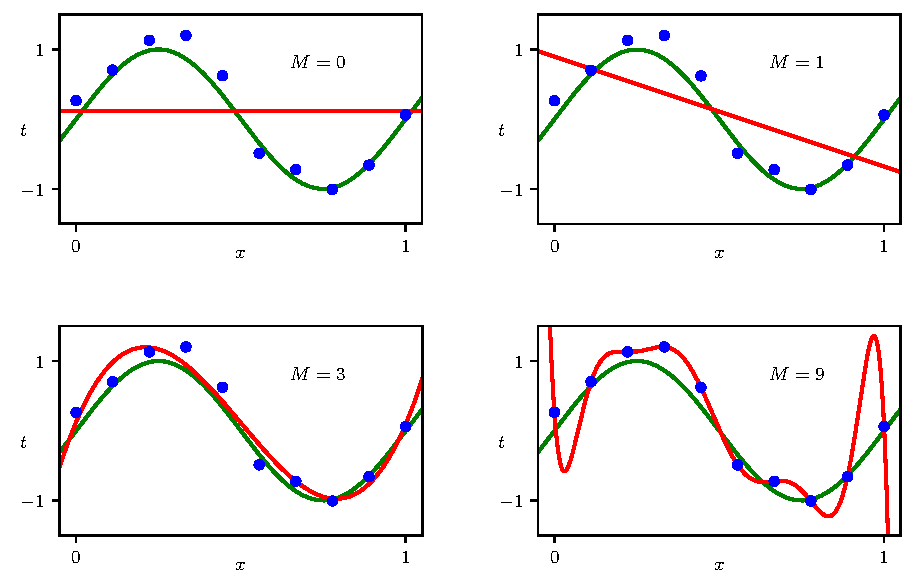
\includegraphics[width=0.88\linewidth]{figures/bishop_polynomial_fits.pdf}
\caption{Polynomial curve fitting with varying degrees of capacity $M \in \{0, 1, 3, 9\}$ on $N = 10$ training samples generated by $t = \sin(2\pi x) + \epsilon$ (blue circles). The green curve represents the true underlying generating function $\sin(2\pi x)$, and the red curve is the least-squares fitted polynomial $y(x, \mathbf{w}) = \sum_{j=0}^M w_j x^j$. For $M = 0$ and $M = 1$, the model underfits (high bias), unable to represent the non-linear sinusoidal pattern. For $M = 3$, the model achieves an optimal balance between capacity and data size. For $M = 9$, the polynomial has 10 free parameters and passes exactly through every training point ($\hat{R}_N = 0$), but exhibits violent oscillations near the boundary domain (Runge's phenomenon), causing catastrophic overfitting (adapted from Bishop~\cite{bishop2024deep}).}
\label{fig:bishop_polynomial_fits}
\end{figure}

The behavior across the four degrees illustrates the capacity spectrum:
\begin{enumerate}[leftmargin=*]
  \item \textbf{Degree $M = 0$ (Constant model):} The hypothesis is a horizontal flat line $y(x) = w_0$, which simply computes the empirical mean of the target values $t_n$. It has zero ability to reflect the spatial variation of $x$, producing massive underfitting.
  \item \textbf{Degree $M = 1$ (Linear model):} The hypothesis is a straight line $y(x) = w_0 + w_1 x$. While it captures the overall negative downward slope across the middle of $[0, 1]$, it is fundamentally incapable of bending to trace the positive and negative lobes of the sine function. High bias dominates.
  \item \textbf{Degree $M = 3$ (Cubic polynomial):} The cubic model possesses sufficient flexibility ($4$ parameters: $w_0, \dots, w_3$) to capture the inflection point and alternating peaks of $\sin(2\pi x)$, while remaining constrained enough to ignore individual noise perturbations. It achieves an optimal trade-off with excellent generalization.
  \item \textbf{Degree $M = 9$ (9th-degree polynomial):} With $M = 9$, the polynomial has $M + 1 = 10$ free parameters $\mathbf{w} = [w_0, \dots, w_9]^\top$, exactly matching the number of data points $N = 10$. The linear system of Normal Equations has a unique exact interpolating solution: the fitted red curve passes \textbf{exactly through every single data point}, yielding $\hat{R}_{\text{train}}(h) = 0$.
  
  However, between the data points—and especially near the boundaries of the interval $[0, 1]$—the curve oscillates wildly, swinging violently into positive and negative extremes. This explosive instability is the classical numerical manifestation known as \textbf{Runge's phenomenon} in high-degree polynomial interpolation. At test time, any point sampled slightly off the training nodes incurs a huge prediction error.
\end{enumerate}

\paragraph{The root mechanical symptom of overfitting: Exploding weight magnitudes.}
Why does the degree-9 polynomial oscillate so violently? When we inspect the numerical values of the optimal weight vector $\mathbf{w}^*$ as $M$ increases, a striking structural pattern emerges:
\begin{itemize}[noitemsep]
  \item For $M = 1$: Weights remain modest: $w_0 \approx 0.8$, $w_1 \approx -1.3$.
  \item For $M = 3$: Weights are comfortably bounded: $w_0 \approx 0.3$, $w_1 \approx 4.9$, $w_2 \approx -10.8$, $w_3 \approx 5.6$.
  \item For $M = 9$: The weights \textbf{explode by multiple orders of magnitude} (reaching magnitudes exceeding $10^5$), alternating between massive positive and negative values.
\end{itemize}
To pass precisely through 10 arbitrarily perturbed points, the high-degree polynomial must execute aggressive, steep turns. A function can only change its slope drastically over minuscule horizontal distances $\Delta x$ if its derivative is enormous, which directly requires astronomical polynomial coefficients $w_j$.

This mathematical realization provides the direct bridge to modern machine learning regularization: if overfitting is mechanically driven by uncontrolled parameter explosion, we can prevent overfitting by penalizing large weight vectors—a technique formalized in Section~\ref{sec:regularization_theory}.

\subsection{Model validation protocols and the Golden Rule of Machine Learning}
\label{sec:validation_protocols}

To detect and prevent overfitting, a machine learner must establish disciplined data splitting protocols.

\paragraph{The Train-Validation-Test partition.}
When a dataset $\mathcal{D}_N$ is provided, it must be partitioned into three strictly isolated subsets:
\begin{equation}
\mathcal{D}_{\text{train}} \quad (60\% - 70\%), \quad \mathcal{D}_{\text{val}} \quad (15\% - 20\%), \quad \mathcal{D}_{\text{test}} \quad (15\% - 20\%).
\end{equation}
\begin{itemize}[noitemsep]
  \item $\mathcal{D}_{\text{train}}$ (Training Set): Used exclusively to fit internal model parameters (e.g., weights $\mathbf{w}$ via gradient descent or least squares).
  \item $\mathcal{D}_{\text{val}}$ (Validation Set): Used to tune \textbf{hyperparameters} (e.g., polynomial degree, learning rate $\eta$, regularization weight $\lambda$) and perform model selection across competing architectures.
  \item $\mathcal{D}_{\text{test}}$ (Test Set): Used exclusively for the final evaluation of generalization performance at deployment time.
\end{itemize}

\paragraph{The Cardinal Rule of Machine Learning.}
In oral examinations, a strict imperative frequently emphasized is the \textbf{Cardinal Rule of Machine Learning}:
\begin{examinsight}[The Cardinal Rule of Machine Learning: Never Touch the Test Set!]
\textbf{Never, EVER use the test set for model selection, hyperparameter tuning, or early stopping!}\\
Using the test set to choose model hyperparameters is statistical cheating. It leaks test information into the training loop, invalidating the i.i.d. assumption and producing severely over-optimistic performance claims that fail when the system is deployed in the real world. The test set must remain locked in a vault, evaluated exactly once at the conclusion of all model design.
\end{examinsight}

\subsection{$k$-Fold and Leave-One-Out cross-validation}
\label{sec:cross_validation}

When the available dataset is small, sequestering a fixed validation set severely reduces the data available for model training. To maximize data efficiency while maintaining rigorous validation, we use \textbf{$k$-Fold Cross-Validation}:
\begin{enumerate}
  \item Partition the training data into $k$ equal-sized disjoint subsets (folds): $\mathcal{D}_1, \mathcal{D}_2, \dots, \mathcal{D}_k$.
  \item Perform $k$ training rounds. In round $i \in \{1, \dots, k\}$:
  \begin{itemize}[noitemsep]
    \item Train the candidate model on the remaining $k-1$ folds: $\bigcup_{j \ne i} \mathcal{D}_j$.
    \item Evaluate empirical validation risk on the held-out fold: $\hat{R}_{\text{val}}^{(i)} = \hat{R}(h; \mathcal{D}_i)$.
  \end{itemize}
  \item Compute the cross-validation performance estimate by averaging across all $k$ rounds:
  \begin{equation}
  \hat{R}_{\text{CV}} = \frac{1}{k} \sum_{i=1}^k \hat{R}_{\text{val}}^{(i)}.
  \label{eq:k_fold_cv_average}
  \end{equation}
\end{enumerate}
Typical choices are $k = 5$ or $k = 10$. 

\paragraph{Leave-One-Out Cross-Validation (LOOCV).}
In the extreme limit where $k = N$ (the total number of training samples):
\begin{itemize}[noitemsep]
  \item Each round trains on $N - 1$ samples and validates on the single remaining sample.
  \item This is repeated $N$ times, averaging errors across all points.
  \item LOOCV provides an almost unbiased estimate of true risk, but is computationally expensive ($O(N)$ full training runs).
\end{itemize}

\subsection{Regularization as a learning solution to overfitting}
\label{sec:regularization_theory}

Cross-validation allows us to select hyperparameters, but how do we prevent a complex model from overfitting directly during optimization? The answer is \textbf{Regularization}: augmenting the empirical risk objective with a penalty that penalizes model complexity.

The regularized empirical risk objective is:
\begin{equation}
\hat{R}_{\text{reg}}(h) \triangleq \hat{R}_N(h) + \lambda \Omega(h) = \frac{1}{N}\sum_{i=1}^N \ell(h(\mathbf{x}_i), y_i) + \lambda \Omega(\mathbf{w}),
\label{eq:regularized_objective}
\end{equation}
where $\Omega(\mathbf{w})$ is a complexity regularizer and $\lambda \ge 0$ is the \textbf{regularization strength} hyperparameter:
\begin{itemize}[noitemsep]
  \item If $\lambda = 0$: Reverts to unconstrained ERM, risking severe overfitting.
  \item If $\lambda \to \infty$: The optimization ignores training data completely, forcing all weights to zero and causing severe underfitting.
  \item Intermediate $\lambda$: Balances empirical fitting fidelity against parameter simplicity.
\end{itemize}

The two canonical forms of regularization in machine learning are:
\begin{enumerate}
  \item \textbf{$L_2$ Regularization (Ridge / Weight Decay)}:
  \begin{equation}
  \Omega(\mathbf{w}) = \frac{1}{2} \|\mathbf{w}\|_2^2 = \frac{1}{2} \sum_{j=1}^d w_j^2.
  \label{eq:l2_regularization}
  \end{equation}
  Drives weight magnitudes smoothly toward zero; prevents any single feature coordinate from exerting disproportionate influence; mathematically equivalent to a zero-mean Gaussian prior.
  \item \textbf{$L_1$ Regularization (Lasso)}:
  \begin{equation}
  \Omega(\mathbf{w}) = \|\mathbf{w}\|_1 = \sum_{j=1}^d |w_j|.
  \label{eq:l1_regularization}
  \end{equation}
  Due to the non-differentiable sharp corners of the $L_1$ ball at coordinate axes, Lasso drives non-essential weights to \textbf{identically zero}, performing automatic feature selection and producing sparse models.
\end{enumerate}

---

\section{Linear predictors, least squares regression, and basis expansion}
\label{sec:linear_predictors_and_least_squares}

\subsection{Linear predictors in 1D and multi-dimensional space}
\label{sec:linear_predictors_formulation}

A \textbf{linear predictor} models the relationship between feature input $\mathbf{x}$ and target $y$ as an affine combination of coordinates:
\begin{itemize}
  \item \textbf{One-Dimensional Predictor}: When the input space is scalar ($\mathcal{X} = \mathbb{R}$), the hypothesis is a straight line:
  \begin{equation}
  \hat{y} = h_{(w,b)}(x) = w x + b,
  \label{eq:linear_predictor_1d}
  \end{equation}
  where $w \in \mathbb{R}$ is the slope weight and $b \in \mathbb{R}$ is the bias offset (y-intercept).
  \item \textbf{Multi-Dimensional Predictor}: When inputs are $d$-dimensional feature vectors ($\mathbf{x} \in \mathbb{R}^d$), the hypothesis is an affine hyperplane:
  \begin{equation}
  \hat{y} = h_{(\mathbf{w},b)}(\mathbf{x}) = \mathbf{w}^\top \mathbf{x} + b = \sum_{j=1}^d w_j x_j + b,
  \label{eq:linear_predictor_multid}
  \end{equation}
  where $\mathbf{w} = [w_1, \dots, w_d]^\top \in \mathbb{R}^d$ is the weight parameter vector.
\end{itemize}

\begin{figure}[htbp]
\centering
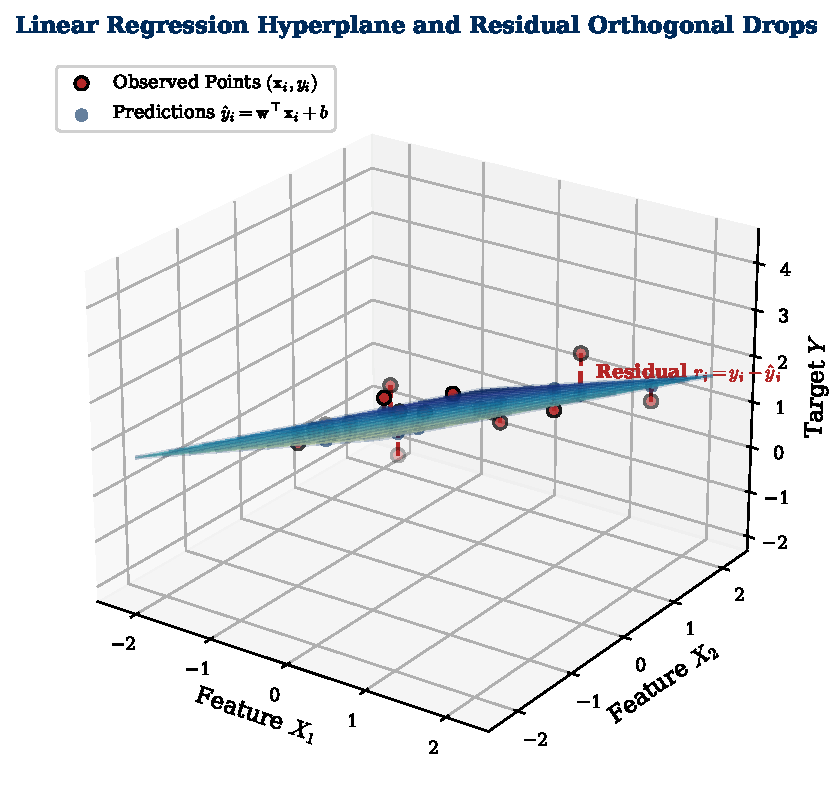
\includegraphics[width=0.72\linewidth]{figures/linear_plane_3d.pdf}
\caption{Geometric representation of a linear predictor for two-dimensional inputs $\mathbf{x} = [x_1, x_2]^\top \in \mathbb{R}^2$ ($h(\mathbf{x}) = w_1 x_1 + w_2 x_2 + b$). In regression, the hypothesis corresponds to a 2D affine hyperplane (colored grid) embedded in 3D feature-target space $(X_1, X_2, Y)$. The observed training instances $(\mathbf{x}_i, y_i)$ are plotted as red spheres, and the vertical drop segments represent the individual residuals $r_i = y_i - \hat{y}_i$ measuring the vertical error between observations and the regression surface.}
\label{fig:linear_plane_3d}
\end{figure}

\paragraph{Geometric interpretation of hyperplanes.}
In classification and regression, the affine equation $\mathbf{w}^\top \mathbf{x} + b = 0$ defines a $(d-1)$-dimensional \textbf{hyperplane}:
\begin{itemize}[noitemsep]
  \item The weight vector $\mathbf{w}$ is the \textbf{orthogonal normal vector} to the hyperplane, pointing toward the positive half-space where $\mathbf{w}^\top \mathbf{x} + b > 0$.
  \item The bias parameter $b$ dictates the orthogonal distance from the coordinate origin to the hyperplane: $\text{distance} = \frac{|b|}{\|\mathbf{w}\|_2}$. If $b = 0$, the hyperplane passes directly through the coordinate origin.
\end{itemize}

\subsection{The Least Squares criterion and matrix-vector formulation}
\label{sec:least_squares_criterion}

For continuous regression, the canonical performance metric is the \textbf{squared loss} $\ell(\hat{y}, y) = \frac{1}{2}(\hat{y} - y)^2$. Under the Empirical Risk Minimization (ERM) framework, the \textbf{Least Squares (LSQ)} criterion searches for the parameter tuple $(\mathbf{w}, b)$ that minimizes the sum (or average) of squared vertical distances between observed training targets $y_i$ and model predictions $\hat{y}_i = h(\mathbf{x}_i)$:
\begin{equation}
J(\mathbf{w}, b) = \frac{1}{2} \sum_{i=1}^N \left( \mathbf{w}^\top \mathbf{x}_i + b - y_i \right)^2.
\label{eq:least_squares_sum_form}
\end{equation}

\paragraph{The geometric meaning of ``Least Squares''.}
\Cref{fig:least_squares_criterion_geometry} illustrates the mechanics of the Least Squares criterion for a 1D linear predictor:
\begin{enumerate}[noitemsep]
  \item For each observed data point $(x_i, y_i)$, the model predicts $\hat{y}_i = wx_i + b$ along the dashed regression line.
  \item The vertical deviation is the \textbf{residual error}:
  \begin{equation}
  r_i \triangleq y_i - \hat{y}_i = y_i - (wx_i + b).
  \label{eq:residual_error_def}
  \end{equation}
  \item The squared loss $\ell_i = r_i^2$ corresponds literally to the \textbf{area of a geometric square} with side length $|r_i|$. The name \emph{Least Squares} originates from the objective of finding the line orientation that minimizes the total aggregate area of all shaded squares.
  \item Once the optimal parameters $(w^*, b^*)$ are learned, the model serves as an inference engine: given any new, unseen query feature $x_0$, the predictor projects $x_0$ vertically onto the fitted line to output the predicted target $\hat{y}_0 = w^* x_0 + b^*$.
\end{enumerate}

\begin{figure}[htbp]
\centering
\begin{tikzpicture}[scale=1.05]
  % Axes
  \draw[-{Stealth[length=2.5mm]}, thick] (0, 0) -- (11.0, 0) node[below=1.5mm, font=\small\sffamily] {Feature input $x$};
  \draw[-{Stealth[length=2.5mm]}, thick] (0, 0) -- (0, 6.6) node[left=1.5mm, font=\small\sffamily] {Target output $y$};
  
  % Bias intercept on y-axis
  \draw[thick] (-0.1, 1.2) -- (0.1, 1.2) node[left=2mm, font=\small\bfseries\sffamily, text=politoNavy] {Intercept $b$};
  
  % Regression line: y = 0.55*x + 1.2
  \draw[very thick, dashed, examred] (0.2, 1.31) -- (9.8, 6.59) 
    node[pos=0.96, above left=1mm, font=\small\bfseries\sffamily, text=examred] {$\hat{y} = wx + b$};

  % Geometric square areas for residuals (r_i^2)
  % Point 1: x=1.6, y=1.4, yhat=2.08, r=-0.68
  \fill[deepblue!15, draw=deepblue!60, thin] (1.6, 1.4) rectangle (1.6 + 0.68, 2.08);
  % Point 2: x=2.8, y=3.7, yhat=2.74, r=+0.96
  \fill[deepblue!15, draw=deepblue!60, thin] (2.8, 2.74) rectangle (2.8 + 0.96, 3.7);
  % Point 3: x=4.3, y=2.9, yhat=3.565, r=-0.665
  \fill[deepblue!15, draw=deepblue!60, thin] (4.3, 2.9) rectangle (4.3 + 0.665, 3.565);
  % Point 4: x=7.0, y=5.8, yhat=5.05, r=+0.75
  \fill[deepblue!15, draw=deepblue!60, thin] (7.0, 5.05) rectangle (7.0 + 0.75, 5.8);
  % Point 5: x=8.3, y=5.1, yhat=5.765, r=-0.665
  \fill[deepblue!15, draw=deepblue!60, thin] (8.3, 5.1) rectangle (8.3 + 0.665, 5.765);

  % Residual vertical lines
  \draw[thick, deepblue] (1.6, 1.4) -- (1.6, 2.08);
  \draw[thick, deepblue] (2.8, 3.7) -- (2.8, 2.74);
  \draw[thick, deepblue] (4.3, 2.9) -- (4.3, 3.565);
  \draw[thick, deepblue] (7.0, 5.8) -- (7.0, 5.05);
  \draw[thick, deepblue] (8.3, 5.1) -- (8.3, 5.765);

  % Fitted predictions (red dots on the line)
  \foreach \coord in {(1.6, 2.08), (2.8, 2.74), (4.3, 3.565), (7.0, 5.05), (8.3, 5.765)} {
    \fill[examred] \coord circle (1.8pt);
  }

  % Training points (xi, yi) (blue dots)
  \foreach \coord in {(1.6, 1.4), (2.8, 3.7), (4.3, 2.9), (7.0, 5.8), (8.3, 5.1)} {
    \fill[politoNavy] \coord circle (2.8pt);
    \draw[black, thick] \coord circle (2.8pt);
  }

  % Annotation for Training sample (pointing to Point 2)
  \draw[-{Stealth[length=1.5mm]}, thick, politoNavy] (1.8, 4.7) node[above, font=\footnotesize\bfseries\sffamily, text=politoNavy] {Training sample $(x_i, y_i)$} -- (2.7, 3.8);

  % Annotation for Residual and Squared Loss (pointing to Point 4)
  \draw[-{Stealth[length=1.5mm]}, thick, deepblue] (8.5, 5.4) -- (7.8, 5.4) 
    node[pos=0, right=1mm, font=\scriptsize\sffamily, align=left, text=deepblue] {
      \textbf{Vertical residual:}\\
      $r_i = y_i - \hat{y}_i = y_i - (wx_i + b)$\\[0.5ex]
      \textbf{Squared loss area:}\\
      $\ell_i = (y_i - \hat{y}_i)^2 = r_i^2$
    };

  % Query prediction x0
  \draw[thick, dashed, deepdiveTeal] (5.6, 0) -- (5.6, 4.28) -- (0, 4.28);
  \fill[deepdiveTeal] (5.6, 4.28) circle (2.8pt);
  \draw[black, thick] (5.6, 4.28) circle (2.8pt);
  \draw[thick] (5.6, 0.1) -- (5.6, -0.1) node[below=1mm, font=\small\bfseries\sffamily, text=deepdiveTeal] {Query $x_0$};
  \draw[thick] (0.1, 4.28) -- (-0.1, 4.28) node[left=1mm, font=\small\bfseries\sffamily, text=deepdiveTeal] {$\hat{y}_0 = h(x_0)$};
  \node[anchor=south east, font=\scriptsize\bfseries\sffamily, text=deepdiveTeal] at (5.55, 4.35) {Prediction $\hat{y}_0 = wx_0 + b$};

  % Summary formula callout
  \node[rectangle, draw=black!70, fill=white, rounded corners=1mm, font=\footnotesize\sffamily, align=center] at (6.5, 1.5) {
    \textbf{\color{politoNavy}Least Squares (LSQ) Fitting Criterion}:\\[0.5ex]
    $h_{\text{LSQ}} = \argmin_{w, b} \dfrac{1}{N} \sum_{i=1}^N \underbrace{\left( y_i - (w x_i + b) \right)^2}_{\text{Sum of squared residual areas } r_i^2}$
  };
\end{tikzpicture}
\caption{The geometry of linear predictors and the Least Squares (LSQ) criterion in one dimension. The hypothesis $\hat{y} = wx + b$ seeks parameters $(w, b)$ that minimize the aggregate sum of squared vertical residuals (represented by the shaded square areas $r_i^2$). For any new query input $x_0$, the model outputs prediction $\hat{y}_0 = h(x_0) = wx_0 + b$ via vertical projection onto the fitted regression line.}
\label{fig:least_squares_criterion_geometry}
\end{figure}

\paragraph{The bias absorption trick.}
To streamline matrix calculus, we absorb the scalar bias $b$ into the weight vector by augmenting each feature vector with a dummy constant coordinate of 1:
\begin{equation}
\mathbf{x}' \triangleq \begin{bmatrix} 1 \\ \mathbf{x} \end{bmatrix} = \begin{bmatrix} 1 \\ x_1 \\ \vdots \\ x_d \end{bmatrix} \in \mathbb{R}^{d+1}, \quad \mathbf{w}' \triangleq \begin{bmatrix} b \\ \mathbf{w} \end{bmatrix} = \begin{bmatrix} b \\ w_1 \\ \vdots \\ w_d \end{bmatrix} \in \mathbb{R}^{d+1}.
\label{eq:bias_absorption_trick}
\end{equation}
Under this homogeneous notation, $\mathbf{w}'^\top \mathbf{x}' = b \cdot 1 + \mathbf{w}^\top \mathbf{x} = \mathbf{w}^\top \mathbf{x} + b$. For the remainder of this derivation, we assume $\mathbf{X}$ and $\mathbf{w}$ represent the augmented coordinates.

We construct the \textbf{Design Matrix} $\mathbf{X} \in \mathbb{R}^{N \times (d+1)}$ by stacking all $N$ augmented sample vectors as rows, and the target vector $\mathbf{y} \in \mathbb{R}^N$:
\begin{equation}
\mathbf{X} = \begin{bmatrix} \mathbf{x}_1^\top \\ \mathbf{x}_2^\top \\ \vdots \\ \mathbf{x}_N^\top \end{bmatrix} = \begin{bmatrix} 1 & x_{11} & \dots & x_{1d} \\ 1 & x_{21} & \dots & x_{2d} \\ \vdots & \vdots & \ddots & \vdots \\ 1 & x_{N1} & \dots & x_{Nd} \end{bmatrix}, \quad \mathbf{y} = \begin{bmatrix} y_1 \\ y_2 \\ \vdots \\ y_N \end{bmatrix}.
\label{eq:design_matrix_form}
\end{equation}
The vector of model predictions across all $N$ training samples is simply the matrix-vector product $\hat{\mathbf{y}} = \mathbf{X}\mathbf{w} \in \mathbb{R}^N$. The empirical loss in compact matrix notation becomes:
\begin{equation}
J(\mathbf{w}) = \frac{1}{2} \|\mathbf{X}\mathbf{w} - \mathbf{y}\|_2^2 = \frac{1}{2} (\mathbf{X}\mathbf{w} - \mathbf{y})^\top (\mathbf{X}\mathbf{w} - \mathbf{y}).
\label{eq:least_squares_matrix_objective}
\end{equation}

\subsection{Analytical derivation of the Normal Equations via matrix calculus}
\label{sec:normal_equations_derivation}

Because $J(\mathbf{w})$ is a convex quadratic function of $\mathbf{w}$, its global minimum occurs where the gradient vector with respect to $\mathbf{w}$ vanishes: $\nabla_{\mathbf{w}} J(\mathbf{w}) = \mathbf{0}$.

\begin{proof}[Analytical Derivation of the Normal Equations]
Expanding the quadratic form in Equation~\eqref{eq:least_squares_matrix_objective}:
\begin{align}
J(\mathbf{w}) &= \frac{1}{2} \left( (\mathbf{X}\mathbf{w})^\top - \mathbf{y}^\top \right) (\mathbf{X}\mathbf{w} - \mathbf{y}) \nonumber \\
&= \frac{1}{2} \left( \mathbf{w}^\top \mathbf{X}^\top \mathbf{X} \mathbf{w} - \mathbf{w}^\top \mathbf{X}^\top \mathbf{y} - \mathbf{y}^\top \mathbf{X} \mathbf{w} + \mathbf{y}^\top \mathbf{y} \right).
\end{align}
Because $\mathbf{w}^\top \mathbf{X}^\top \mathbf{y}$ is a scalar, it equals its own transpose: $\mathbf{w}^\top \mathbf{X}^\top \mathbf{y} = (\mathbf{w}^\top \mathbf{X}^\top \mathbf{y})^\top = \mathbf{y}^\top \mathbf{X} \mathbf{w}$. Combining the cross-terms:
\begin{equation}
J(\mathbf{w}) = \frac{1}{2} \mathbf{w}^\top (\mathbf{X}^\top \mathbf{X}) \mathbf{w} - \mathbf{w}^\top (\mathbf{X}^\top \mathbf{y}) + \frac{1}{2} \mathbf{y}^\top \mathbf{y}.
\label{eq:expanded_matrix_loss}
\end{equation}

Now, compute the vector derivative $\nabla_{\mathbf{w}} J(\mathbf{w})$ using standard matrix calculus identities ($\nabla_{\mathbf{w}} (\mathbf{w}^\top \mathbf{A} \mathbf{w}) = (\mathbf{A} + \mathbf{A}^\top)\mathbf{w} = 2\mathbf{A}\mathbf{w}$ for symmetric $\mathbf{A} = \mathbf{X}^\top \mathbf{X}$, and $\nabla_{\mathbf{w}} (\mathbf{w}^\top \mathbf{b}) = \mathbf{b}$):
\begin{equation}
\nabla_{\mathbf{w}} J(\mathbf{w}) = \mathbf{X}^\top \mathbf{X} \mathbf{w} - \mathbf{X}^\top \mathbf{y}.
\label{eq:least_squares_gradient}
\end{equation}
Setting the gradient identically to zero:
\begin{equation}
\mathbf{X}^\top \mathbf{X} \mathbf{w} - \mathbf{X}^\top \mathbf{y} = \mathbf{0}.
\end{equation}
This yields the celebrated \textbf{Normal Equations}:
\begin{equation}
\mathbf{X}^\top \mathbf{X} \mathbf{w} = \mathbf{X}^\top \mathbf{y}.
\label{eq:normal_equations}
\end{equation}
Assuming the square matrix $\mathbf{X}^\top \mathbf{X} \in \mathbb{R}^{(d+1) \times (d+1)}$ is invertible (full column rank), multiplying both sides by $(\mathbf{X}^\top \mathbf{X})^{-1}$ gives the unique closed-form \textbf{Ordinary Least Squares (OLS)} estimator:
\begin{equation}
\mathbf{w}^* = (\mathbf{X}^\top \mathbf{X})^{-1} \mathbf{X}^\top \mathbf{y}.
\label{eq:ols_closed_form}
\end{equation}
\end{proof}

\subsection{Regularized Least Squares: Closed-form Ridge Regression}
\label{sec:ridge_regression_derivation}

What happens if $\mathbf{X}^\top \mathbf{X}$ is not invertible? This failure occurs when:
\begin{itemize}[noitemsep]
  \item Features are collinear (redundant columns in $\mathbf{X}$).
  \item The number of features exceeds the number of training samples ($d > N$).
\end{itemize}
To guarantee invertibility and prevent overfitting, we add $L_2$ regularization:
\begin{equation}
J_{\text{ridge}}(\mathbf{w}) = \frac{1}{2} \|\mathbf{X}\mathbf{w} - \mathbf{y}\|_2^2 + \frac{\lambda}{2} \|\mathbf{w}\|_2^2, \quad \lambda > 0.
\label{eq:ridge_objective}
\end{equation}

Computing the gradient of the regularized objective:
\begin{equation}
\nabla_{\mathbf{w}} J_{\text{ridge}}(\mathbf{w}) = \mathbf{X}^\top \mathbf{X} \mathbf{w} - \mathbf{X}^\top \mathbf{y} + \lambda \mathbf{w} = (\mathbf{X}^\top \mathbf{X} + \lambda \mathbf{I}) \mathbf{w} - \mathbf{X}^\top \mathbf{y}.
\end{equation}
Setting the gradient to zero:
\begin{equation}
(\mathbf{X}^\top \mathbf{X} + \lambda \mathbf{I}) \mathbf{w} = \mathbf{X}^\top \mathbf{y}.
\label{eq:ridge_normal_equations}
\end{equation}
Multiplying by the inverse yields the closed-form \textbf{Ridge Regression} solution:
\begin{equation}
\mathbf{w}^*_{\text{ridge}} = (\mathbf{X}^\top \mathbf{X} + \lambda \mathbf{I})^{-1} \mathbf{X}^\top \mathbf{y}.
\label{eq:ridge_closed_form}
\end{equation}

\paragraph{Mathematical guarantee of invertibility.}
Why is $(\mathbf{X}^\top \mathbf{X} + \lambda \mathbf{I})$ guaranteed to be invertible for any $\lambda > 0$?
\begin{itemize}[noitemsep]
  \item The matrix $\mathbf{X}^\top \mathbf{X}$ is symmetric and positive semi-definite: all its eigenvalues satisfy $\mu_i \ge 0$.
  \item Adding $\lambda \mathbf{I}$ shifts every eigenvalue strictly by $\lambda$:
  \begin{equation}
  \operatorname{eig}_i(\mathbf{X}^\top \mathbf{X} + \lambda \mathbf{I}) = \mu_i + \lambda \ge \lambda > 0.
  \end{equation}
  \item Because all eigenvalues are strictly positive ($\lambda > 0$), the determinant $\det(\mathbf{X}^\top \mathbf{X} + \lambda \mathbf{I}) = \prod_i (\mu_i + \lambda) > 0$. The matrix is strictly \textbf{positive definite and guaranteed invertible}, stabilizing matrix conditioning even in high-dimensional $d \gg N$ regimes.
\end{itemize}

\subsection{Beyond linear models: Non-linear fitting via polynomial basis expansion}
\label{sec:basis_expansion}

Linear regression appears restricted to planar surfaces. Can we use linear regression to fit arbitrary non-linear curves?

The answer is yes, through the technique of \textbf{Basis Function Expansion}. Instead of operating directly on the raw input scalar $x \in \mathbb{R}$, we map $x$ into a high-dimensional feature space using fixed non-linear basis transformations:
\begin{equation}
\boldsymbol{\phi}(x) = [1, \phi_1(x), \phi_2(x), \dots, \phi_p(x)]^\top \in \mathbb{R}^{p+1}.
\label{eq:basis_expansion_mapping}
\end{equation}
For polynomial regression of degree $p$:
\begin{equation}
\boldsymbol{\phi}(x) = [1, x, x^2, x^3, \dots, x^p]^\top.
\label{eq:polynomial_basis_vector}
\end{equation}
The prediction model becomes:
\begin{equation}
h(x) = \mathbf{w}^\top \boldsymbol{\phi}(x) = w_0 + w_1 x + w_2 x^2 + \dots + w_p x^p.
\label{eq:polynomial_linear_in_parameters}
\end{equation}

Crucially, \textbf{$h(x)$ is non-linear with respect to the input $x$, but strictly linear with respect to the parameters $\mathbf{w}$!} 

Therefore, we can construct the feature matrix $\mathbf{\Phi} \in \mathbb{R}^{N \times (p+1)}$ where row $i$ is $\boldsymbol{\phi}(x_i)^\top$, and solve for the optimal weights using the exact same closed-form Normal Equations derived in Equation~\eqref{eq:ols_closed_form}:
\begin{equation}
\mathbf{w}^* = (\mathbf{\Phi}^\top \mathbf{\Phi})^{-1} \mathbf{\Phi}^\top \mathbf{y}.
\label{eq:basis_normal_equations}
\end{equation}

\paragraph{The conceptual bridge to Chapter~\ref{sec:optimization_and_gradient_descent}: The dual motivation for Gradient Descent.}
The closed-form Normal Equations $\mathbf{w}^* = (\mathbf{X}^\top \mathbf{X})^{-1}\mathbf{X}^\top \mathbf{y}$ (and its regularized counterpart in Equation~\eqref{eq:ridge_closed_form}) represent an elegant analytical result. However, students must recognize that the existence of this closed-form solution is a \textbf{rare, fortunate mathematical coincidence} rather than the general norm in machine learning. 

Analytically reducing the stationary condition $\nabla_{\mathbf{w}} J(\mathbf{w}) = \mathbf{0}$ to a linear matrix equation solvable via direct matrix inversion ($\mathbf{A}\mathbf{w} = \mathbf{b} \implies \mathbf{w}^* = \mathbf{A}^{-1}\mathbf{b}$) holds as an exact equivalence ($\iff$) if and only if two conditions coincide simultaneously:
\begin{enumerate}[noitemsep]
  \item The predictor $h(\mathbf{x})$ is strictly \textbf{linear in its parameter vector} $\mathbf{w}$ (as in linear regression or fixed basis expansions).
  \item The loss function $\ell(\hat{y}, y)$ is strictly \textbf{quadratic in its prediction} $\hat{y}$ (such as standard squared error, weighted least squares, or ridge regularizers).
\end{enumerate}
Only under this exact pairing does the empirical objective $J(\mathbf{w})$ form a purely quadratic polynomial in $\mathbf{w}$, ensuring that its gradient $\nabla_{\mathbf{w}} J(\mathbf{w}) = \mathbf{A}\mathbf{w} - \mathbf{b}$ is strictly \emph{affine} (linear in $\mathbf{w}$), which yields a linear algebraic system of equations solvable by matrix inversion. (Note that for the existence of closed-form solutions in general, this condition is only sufficient ($\impliedby$) but not necessary, as analytical closed forms also arise in generative models like Naive Bayes or median estimation under $L_1$ loss; however, for solvability specifically via \emph{linear matrix inversion}, it is an exact $\iff$ equivalence).

In modern machine learning, this algebraic convenience collapses across two fundamental dimensions, establishing the \textbf{dual motivation} for first-order numerical optimization:
\begin{itemize}
  \item \textbf{1. Mathematical Necessity (Non-solvability for General and Non-Convex Losses):} 
  The moment we step outside quadratic loss, setting the gradient to zero no longer yields a linear system:
  \begin{itemize}[noitemsep]
    \item \emph{Convex, non-quadratic losses:} Even for elementary linear models, if we adopt Cross-Entropy (Logistic Loss) for classification, setting $\nabla_{\mathbf{w}} J(\mathbf{w}) = \sum_{i=1}^N (\sigma(\mathbf{w}^\top \mathbf{x}_i) - y_i)\mathbf{x}_i = \mathbf{0}$ produces a coupled system of \textbf{transcendental, non-linear equations}. No algebraic matrix inversion can ever isolate $\mathbf{w}^*$, despite the objective being strictly convex. The same analytical impossibility applies to Hinge loss (SVMs) and $L_1$ loss.
    \item \emph{Non-convex landscapes and Neural Networks:} When models introduce non-linear parameter compositions (as in deep neural networks $h_{\mathbf{w}}(\mathbf{x}) = \mathbf{W}_L \sigma(\mathbf{W}_{L-1} \dots \sigma(\mathbf{W}_1 \mathbf{x}))$), the empirical loss surface $J(\mathbf{w})$ becomes highly non-convex, populated by intricate configurations of local minima, ravines, and saddle points. Here, algebraic inversion is conceptually and mathematically impossible. An iterative algorithm is the \emph{sole viable mechanism} to navigate the landscape.
  \end{itemize}
  
  \item \textbf{2. Computational Intractability (High-Dimensional Scaling):}
  Even in the ideal textbook scenario where a closed-form solution exists (linear model with MSE), evaluating $(\mathbf{X}^\top \mathbf{X})^{-1}\mathbf{X}^\top \mathbf{y}$ is computationally prohibitive for high-dimensional problems:
  \begin{itemize}[noitemsep]
    \item Computing the Gram matrix $\mathbf{X}^\top \mathbf{X}$ requires $\mathcal{O}(N d^2)$ floating-point operations.
    \item Inverting the $(d \times d)$ matrix requires Gaussian elimination or Cholesky factorization scaling cubically as $\mathcal{O}(d^3)$, and demands $\mathcal{O}(d^2)$ memory to store.
    \item When feature representations or neural architectures contain millions or billions of parameters ($d \ge 10^6$), materializing and inverting a $(d \times d)$ matrix exceeds the physical memory and compute capacity of modern computing clusters.
  \end{itemize}
\end{itemize}

Therefore, whether driven by \textbf{mathematical necessity} (non-convex, non-linear, and transcendental loss objectives where closed forms do not exist) or by \textbf{computational necessity} (high-dimensional regimes where matrix inversion is computationally intractable), machine learning must abandon closed-form algebraic solutions. Instead, we must embrace iterative, first-order local optimization: \textbf{Gradient Descent}. 

How to navigate non-linear loss surfaces, escape saddle points, and optimize non-convex objectives iteratively forms the foundational core of Chapter~\ref{sec:optimization_and_gradient_descent}.

\chapter{Linear predictors, generalization, and first-order numerical optimization}
\label{sec:linear_predictors_and_gradient_optimization}
\label{sec:optimization_and_gradient_descent}

In the quest to construct predictive machines from empirical observations, the most natural starting point is the \textbf{linear model}---a hypothesis class that models outputs as affine combinations of input features. Linear models possess an extraordinary mathematical elegance: under the classic squared error criterion, their optimal parameters admit a closed-form, globally optimal analytical solution via the celebrated \textbf{Normal Equations}. 

However, as statistical learning scales to real-world complexities, this apparent simplicity fractures along three profound theoretical and computational fault lines:
\begin{enumerate}[noitemsep,topsep=2pt,parsep=0pt,partopsep=0pt]
  \item \textbf{Generalization and capacity}: When linear models are enriched with non-linear basis expansions (such as high-degree polynomials), they acquire immense expressive capacity. Without principled constraints, they succumb to catastrophic \textbf{overfitting}---memorizing sample noise while losing all predictive power on unseen data.
  \item \textbf{High-dimensional breakdown of closed-form algebra}: Computing analytical matrix inversions requires $\mathcal{O}(D^3)$ computational steps. When the feature dimension $D$ exceeds the number of observations $N$ ($D > N$), the sample covariance matrix becomes strictly singular, causing classical least squares to collapse into an ill-posed system with infinitely many solutions.
  \item \textbf{The regression-to-classification barrier}: When discrete labels replace continuous targets, least squares outputs uncalibrated, unbounded values that violate probability axioms, and remote outliers exert quadratic leverage that destabilizes decision boundaries. Replacing squared error with probabilistic cross-entropy eliminates these pathologies, but destroys the existence of closed-form solutions: setting the gradient to zero yields a transcendental system that \textbf{cannot be inverted algebraically}.
\end{enumerate}

To conquer these barriers, machine learning must abandon closed-form linear algebra and embrace two foundational pillars: \textbf{regularization} (to tame capacity and restore matrix invertibility) and \textbf{iterative numerical optimization} (gradient descent, momentum, and stochastic mini-batch dynamics). This chapter charts this complete intellectual journey from closed-form least squares to modern large-scale optimization.

\section{Linear regression, ordinary least squares, and model capacity}
\label{sec:linear_regression_and_capacity}

In the study of supervised learning, linear models occupy a foundational position as both an intuitive baseline and an analytically tractable laboratory for exploring core statistical principles. By modeling the relationship between input features and continuous targets as an affine transformation, linear regression provides an interpretable mapping whose parameters directly reflect feature importances. Under the classic squared error criterion, the parameter estimation problem achieves a rare and remarkable property in machine learning: it admits an exact, globally optimal analytical closed-form solution via the celebrated Normal Equations, bypassing the need for exploratory numerical search.

\subsection{Ordinary least squares, normal equations, and orthogonal projection}
\label{sec:ols_and_normal_equations}
\label{sec:linear_predictor_formulation}
\label{sec:ols_and_mle}
\label{sec:normal_equations_derivation}
\label{sec:geometric_projection_ols}
\label{sec:ols_computational_complexity}

Consider a supervised regression setting where each input instance is represented as a real-valued feature vector $\vx = [x_1, x_2, \dots, x_D]^\top \in \R^D$, and the associated target variable is continuous $y \in \R$. The \textbf{linear predictor} posits an affine relationship between inputs and targets:
\begin{equation}
h_{\vw, b}(\vx) = \vw^\top \vx + b = \sum_{j=1}^D w_j x_j + b,
\label{eq:linear_predictor_affine}
\end{equation}
where $\vw = [w_1, w_2, \dots, w_D]^\top \in \R^D$ denotes the weight vector (governing the slope or orientation of the predictive hyperplane) and $b \in \R$ denotes the scalar bias (governing the intercept, offsetting the hyperplane from the origin).

To streamline algebraic manipulations and eliminate separate treatment of the bias term, we adopt the standard \textbf{homogeneous coordinate augmentation}. We append a constant $1$ as a dummy feature to the input vector and absorb the bias directly into the parameter vector:
\begin{equation}
\tilde{\vx} \triangleq \begin{bmatrix} \vx \\ 1 \end{bmatrix} \in \R^{D+1}, \quad
\tilde{\vw} \triangleq \begin{bmatrix} \vw \\ b \end{bmatrix} \in \R^{D+1}
\implies h_{\tilde{\vw}}(\tilde{\vx}) = \tilde{\vw}^\top \tilde{\vx}.
\label{eq:homogeneous_coords}
\end{equation}

Given an empirical training dataset consisting of $N$ independently and identically distributed (i.i.d.) observations $\mathcal{D} = \{(\vx_i, y_i)\}_{i=1}^N$, we assemble the inputs into the \textbf{augmented design matrix} $\tilde{\mX} \in \R^{N \times (D+1)}$ and the targets into the target vector $\vy \in \R^N$:
\begin{equation}
\tilde{\mX} = \begin{bmatrix} \tilde{\vx}_1^\top \\ \tilde{\vx}_2^\top \\ \vdots \\ \tilde{\vx}_N^\top \end{bmatrix} = \begin{bmatrix} x_{1,1} & x_{1,2} & \cdots & x_{1,D} & 1 \\ x_{2,1} & x_{2,2} & \cdots & x_{2,D} & 1 \\ \vdots & \vdots & \ddots & \vdots & \vdots \\ x_{N,1} & x_{N,2} & \cdots & x_{N,D} & 1 \end{bmatrix}, \quad
\vy = \begin{bmatrix} y_1 \\ y_2 \\ \vdots \\ y_N \end{bmatrix}.
\label{eq:design_matrix_def}
\end{equation}
In this vectorized matrix notation, the predictions across all $N$ training samples are expressed compactly as the matrix-vector product:
\begin{equation}
\hat{\vy} \triangleq \tilde{\mX}\tilde{\vw} \in \R^N.
\label{eq:vectorized_predictions}
\end{equation}

To determine the optimal parameter vector $\tilde{\vw}^*$, we define an empirical loss metric penalizing discrepancies between model predictions $\hat{y}_i$ and ground-truth targets $y_i$. Under the \textbf{Ordinary Least Squares (OLS)} framework, we adopt the squared error loss $\ell(h(\vx), y) = \frac{1}{2}(h(\vx) - y)^2$. The empirical risk (mean squared error objective) over the training set is:
\begin{equation}
J(\tilde{\vw}) \triangleq \frac{1}{2N} \sum_{i=1}^N \left( \tilde{\vx}_i^\top \tilde{\vw} - y_i \right)^2 = \frac{1}{2N} \|\tilde{\mX}\tilde{\vw} - \vy\|_2^2.
\label{eq:ols_empirical_risk}
\end{equation}

\begin{deepdive}[Probabilistic Derivation of Least Squares from Maximum Likelihood]
Why squared error? In Chapter~2, we proved that minimizing empirical risk under squared loss corresponds to Maximum Likelihood Estimation (MLE) under a conditional Gaussian noise model. Specifically, assume the continuous target $y$ is generated by a deterministic linear mapping corrupted by additive zero-mean Gaussian noise:
\begin{equation}
y = \tilde{\vw}^\top \tilde{\vx} + \epsilon, \quad \text{where } \epsilon \sim \mathcal{N}(0, \sigma^2).
\label{eq:gaussian_noise_model}
\end{equation}
The conditional probability density of observing target $y$ given input $\tilde{\vx}$ is therefore:
\begin{equation}
p(y \mid \tilde{\vx}; \tilde{\vw}, \sigma^2) = \frac{1}{\sqrt{2\pi \sigma^2}} \exp\left( -\frac{(y - \tilde{\vw}^\top \tilde{\vx})^2}{2\sigma^2} \right).
\label{eq:conditional_gaussian_density}
\end{equation}
Assuming observations are drawn i.i.d., the total conditional log-likelihood of the dataset $\mathcal{D}$ evaluates to:
\begin{align}
\log p(\vy \mid \tilde{\mX}; \tilde{\vw}, \sigma^2) &= \sum_{i=1}^N \log p(y_i \mid \tilde{\vx}_i; \tilde{\vw}, \sigma^2) \nonumber \\
&= -\frac{N}{2} \log(2\pi\sigma^2) - \frac{1}{2\sigma^2} \sum_{i=1}^N \left( y_i - \tilde{\vw}^\top \tilde{\vx}_i \right)^2 \nonumber \\
&= -\frac{N}{2} \log(2\pi\sigma^2) - \frac{1}{2\sigma^2} \|\tilde{\mX}\tilde{\vw} - \vy\|_2^2.
\label{eq:log_likelihood_ols}
\end{align}
Because the first term is independent of $\tilde{\vw}$, maximizing the log-likelihood with respect to parameters $\tilde{\vw}$ is mathematically equivalent to minimizing the squared Euclidean norm $\|\tilde{\mX}\tilde{\vw} - \vy\|_2^2$:
\begin{equation}
\hat{\tilde{\vw}}_{\text{MLE}} = \argmax_{\tilde{\vw}} \log p(\vy \mid \tilde{\mX}; \tilde{\vw}, \sigma^2) \equiv \argmin_{\tilde{\vw}} \frac{1}{2N} \|\tilde{\mX}\tilde{\vw} - \vy\|_2^2 = \argmin_{\tilde{\vw}} J(\tilde{\vw}).
\label{eq:mle_equals_ols}
\end{equation}
Thus, ordinary least squares is not merely an arbitrary heuristic: it is the optimal maximum likelihood estimator under homoscedastic Gaussian observation noise.
\end{deepdive}

Because the empirical risk $J(\tilde{\vw})$ is a quadratic function of $\tilde{\vw}$ and its Hessian $\nabla_{\tilde{\vw}}^2 J(\tilde{\vw}) = \frac{1}{N}\tilde{\mX}^\top \tilde{\mX}$ is positive semi-definite (strictly positive definite when $\tilde{\mX}$ has full column rank), the objective is convex and any stationary point is a global minimizer. We can therefore find its exact global minimum by expanding the objective in matrix form and setting its vector gradient to zero.

\begin{proof}[Derivation of the Normal Equations]
Expanding the squared $L_2$ norm:
\begin{align}
J(\tilde{\vw}) &= \frac{1}{2N} (\tilde{\mX}\tilde{\vw} - \vy)^\top (\tilde{\mX}\tilde{\vw} - \vy) \nonumber \\
&= \frac{1}{2N} \left( (\tilde{\vw}^\top \tilde{\mX}^\top - \vy^\top)(\tilde{\mX}\tilde{\vw} - \vy) \right) \nonumber \\
&= \frac{1}{2N} \left( \tilde{\vw}^\top \tilde{\mX}^\top \tilde{\mX} \tilde{\vw} - \tilde{\vw}^\top \tilde{\mX}^\top \vy - \vy^\top \tilde{\mX} \tilde{\vw} + \vy^\top \vy \right).
\label{eq:ols_expansion}
\end{align}
Since $\tilde{\vw}^\top \tilde{\mX}^\top \vy$ is a scalar, it equals its transpose $\vy^\top \tilde{\mX} \tilde{\vw}$. Combining these identical bilinear terms yields:
\begin{equation}
J(\tilde{\vw}) = \frac{1}{2N} \left( \tilde{\vw}^\top \tilde{\mX}^\top \tilde{\mX} \tilde{\vw} - 2 \vy^\top \tilde{\mX} \tilde{\vw} + \vy^\top \vy \right).
\label{eq:ols_compact_expansion}
\end{equation}
We now take the vector derivative with respect to $\tilde{\vw}$. We invoke the two canonical matrix calculus identities:
\begin{equation}
\nabla_{\mathbf{z}} (\mathbf{z}^\top \mA \mathbf{z}) = (\mA + \mA^\top)\mathbf{z} = 2\mA\mathbf{z} \quad (\text{for symmetric } \mA), \qquad \nabla_{\mathbf{z}} (\mathbf{c}^\top \mathbf{z}) = \mathbf{c}.
\label{eq:matrix_calc_rules}
\end{equation}
Applying these identities to Eq.~\eqref{eq:ols_compact_expansion} (where $\tilde{\mX}^\top \tilde{\mX}$ is symmetric):
\begin{equation}
\nabla_{\tilde{\vw}} J(\tilde{\vw}) = \frac{1}{2N} \left( 2 \tilde{\mX}^\top \tilde{\mX} \tilde{\vw} - 2 \tilde{\mX}^\top \vy \right) = \frac{1}{N} \left( \tilde{\mX}^\top \tilde{\mX} \tilde{\vw} - \tilde{\mX}^\top \vy \right).
\label{eq:ols_gradient}
\end{equation}
Setting the gradient to the zero vector $\nabla_{\tilde{\vw}} J(\tilde{\vw}) = \mathbf{0}$ yields the celebrated \textbf{Normal Equations}:
\begin{equation}
\tilde{\mX}^\top \tilde{\mX} \tilde{\vw} = \tilde{\mX}^\top \vy.
\label{eq:normal_equations}
\end{equation}
If the $(D+1) \times (D+1)$ Gram matrix $\tilde{\mX}^\top \tilde{\mX}$ is invertible (non-singular), multiplying both sides by $(\tilde{\mX}^\top \tilde{\mX})^{-1}$ delivers the unique analytical closed-form solution:
\begin{equation}
\tilde{\vw}^* = (\tilde{\mX}^\top \tilde{\mX})^{-1} \tilde{\mX}^\top \vy.
\label{eq:ols_solution}
\end{equation}
The matrix $(\tilde{\mX}^\top \tilde{\mX})^{-1} \tilde{\mX}^\top \triangleq \tilde{\mX}^\dagger \in \R^{(D+1) \times N}$ is the classical \textbf{Moore-Penrose pseudoinverse} of $\tilde{\mX}$ for full column-rank matrices.
\end{proof}

The Normal Equations possess an illuminating geometric interpretation in the $N$-dimensional sample space $\R^N$ (Bishop, 2024; Strang, 2016). 

The target vector $\vy = [y_1, \dots, y_N]^\top$ is an arbitrary point in $\R^N$. Any prediction vector $\hat{\vy} = \tilde{\mX}\tilde{\vw}$ is a linear combination of the columns of the design matrix $\tilde{\mX}$:
\begin{equation}
\hat{\vy} = \tilde{\vw}_1 \tilde{\vx}_{*,1} + \tilde{\vw}_2 \tilde{\vx}_{*,2} + \dots + \tilde{\vw}_{D+1} \tilde{\vx}_{*,D+1} \in \operatorname{col}(\tilde{\mX}),
\label{eq:col_space_comb}
\end{equation}
where $\operatorname{col}(\tilde{\mX}) \subset \R^N$ is the $(D+1)$-dimensional subspace spanned by the column vectors of $\tilde{\mX}$. 

Minimizing the squared Euclidean distance $\|\hat{\vy} - \vy\|_2^2$ means finding the point $\hat{\vy}$ within the subspace $\operatorname{col}(\tilde{\mX})$ that lies closest to the target vector $\vy$. By elementary Euclidean geometry, the shortest distance from an external point to a linear subspace is achieved when the error (residual) vector $\mathbf{e} \triangleq \vy - \hat{\vy}$ is strictly \textbf{orthogonal} to the subspace:
\begin{equation}
\mathbf{e} \perp \operatorname{col}(\tilde{\mX}) \iff \tilde{\vx}_{*,j}^\top \mathbf{e} = 0 \quad \forall j \in \{1, \dots, D+1\} \iff \tilde{\mX}^\top (\vy - \tilde{\mX}\tilde{\vw}^*) = \mathbf{0},
\label{eq:orthogonality_condition}
\end{equation}
which is precisely the Normal Equations $\tilde{\mX}^\top \tilde{\mX} \tilde{\vw}^* = \tilde{\mX}^\top \vy$!

Substituting the optimal weights $\tilde{\vw}^*$ into the prediction vector:
\begin{equation}
\hat{\vy} = \tilde{\mX}\tilde{\vw}^* = \tilde{\mX}(\tilde{\mX}^\top \tilde{\mX})^{-1}\tilde{\mX}^\top \vy \triangleq \mathbf{P}_{\tilde{\mX}} \vy,
\label{eq:projection_matrix}
\end{equation}
where $\mathbf{P}_{\tilde{\mX}} \triangleq \tilde{\mX}(\tilde{\mX}^\top \tilde{\mX})^{-1}\tilde{\mX}^\top \in \R^{N \times N}$ is the \textbf{orthogonal projection operator} (or \textit{hat matrix} $\mathbf{H}$, because it puts the ``hat'' on $\vy$). The projection matrix satisfies:
\begin{enumerate}[noitemsep,topsep=2pt,parsep=0pt,partopsep=0pt]
  \item \textbf{Symmetry}: $\mathbf{P}_{\tilde{\mX}}^\top = (\tilde{\mX}(\tilde{\mX}^\top \tilde{\mX})^{-1}\tilde{\mX}^\top)^\top = \tilde{\mX}(\tilde{\mX}^\top \tilde{\mX})^{-1}\tilde{\mX}^\top = \mathbf{P}_{\tilde{\mX}}$.
  \item \textbf{Idempotency}: $\mathbf{P}_{\tilde{\mX}}^2 = \tilde{\mX}(\tilde{\mX}^\top \tilde{\mX})^{-1}\tilde{\mX}^\top \tilde{\mX}(\tilde{\mX}^\top \tilde{\mX})^{-1}\tilde{\mX}^\top = \tilde{\mX}(\tilde{\mX}^\top \tilde{\mX})^{-1}\tilde{\mX}^\top = \mathbf{P}_{\tilde{\mX}}$. Projecting an already-projected vector leaves it unchanged.
\end{enumerate}

Figure~\ref{fig:ols_orthogonal_projection} visually demonstrates how Ordinary Least Squares computes the unique point $\hat{\vy}$ within the subspace $\operatorname{col}(\tilde{\mX})$ closest to $\vy$.

\begin{figure}[H]
\centering
\begin{tikzpicture}[scale=1.05]
  % Subspace parallelogram (col(\tilde{X}))
  \coordinate (A) at (0.4, 0.3);
  \coordinate (B) at (8.6, 0.3);
  \coordinate (C) at (11.0, 3.1);
  \coordinate (D) at (2.8, 3.1);

  \fill[deepdiveTeal!6] (A) -- (B) -- (C) -- (D) -- cycle;
  \draw[politoNavy!70, thick] (A) -- (B) -- (C) -- (D) -- cycle;

  % Subspace label inside the plane at top-right
  \node[font=\bfseries\sffamily, text=politoNavy, anchor=north east] at (10.8, 2.95) {$\operatorname{col}(\tilde{\mathbf{X}}) \subset \mathbb{R}^N$};
  \node[font=\scriptsize\sffamily, text=politoNavy!80, anchor=north east] at (10.8, 2.55) {$\operatorname{span}\{\tilde{\mathbf{x}}_{*,1}, \dots, \tilde{\mathbf{x}}_{*,D+1}\}$};

  % Origin
  \coordinate (O) at (1.8, 0.9);
  \fill[politoNavy] (O) circle (2.2pt) node[below left=2pt, font=\small\bfseries\sffamily] {$\mathbf{0}$};

  % Spanning column vectors
  \coordinate (X1) at (4.8, 0.9); % along x-axis
  \coordinate (X2) at (3.3, 2.2); % along depth

  \draw[-{Stealth[length=2.5mm]}, thick, politoNavy] (O) -- (X1) 
    node[below=2pt, font=\small\bfseries\sffamily] {$\tilde{\mathbf{x}}_{*,1}$};
  \draw[-{Stealth[length=2.5mm]}, thick, politoNavy] (O) -- (X2) 
    node[above left=1pt, font=\small\bfseries\sffamily] {$\tilde{\mathbf{x}}_{*,2}$};

  % Prediction vector \hat{y} on the plane
  \coordinate (V1) at (4.4, 0.9);
  \coordinate (V2) at (2.9, 1.87);
  \coordinate (P) at (5.5, 1.87);

  % Dashed component lines on the subspace plane
  \draw[densely dashed, politoNavy!45, thick] (V1) -- (P);
  \draw[densely dashed, politoNavy!45, thick] (V2) -- (P);

  % Vector \hat{y}
  \draw[-{Stealth[length=3mm]}, line width=1.6pt, intuitiongreen!80!black] (O) -- (P)
    node[midway, below right=1pt, font=\small\bfseries\sffamily, text=intuitiongreen!80!black] {$\hat{\mathbf{y}} = \tilde{\mathbf{X}}\tilde{\mathbf{w}}^*$};
  \fill[intuitiongreen!80!black] (P) circle (2.2pt) node[below right=2pt, font=\scriptsize\bfseries\sffamily, text=intuitiongreen!80!black] {$\hat{\mathbf{y}}$ (Closest point in $\operatorname{col}(\tilde{\mathbf{X}})$)};

  % Target vector y above the plane
  \coordinate (Y) at (5.5, 5.5);
  \draw[-{Stealth[length=3.2mm]}, line width=1.6pt, deepblue] (O) -- (Y);
  \fill[deepblue] (Y) circle (2.2pt) node[above=3pt, font=\small\bfseries\sffamily, text=deepblue] {$\mathbf{y} \in \mathbb{R}^N$ (Observed target)};

  % Residual vector e = y - \hat{y} (orthogonal to subspace)
  \draw[-{Stealth[length=3.2mm]}, line width=1.6pt, examred] (P) -- (Y)
    node[pos=0.55, right=5pt, font=\small\bfseries\sffamily, text=examred] {$\mathbf{e} = \mathbf{y} - \hat{\mathbf{y}} \perp \operatorname{col}(\tilde{\mathbf{X}})$};

  % Right angle mark at P
  \draw[thick, examred!90!black] ($(P) + (-0.35, 0)$) -- ($(P) + (-0.35, 0.35)$) -- ($(P) + (0, 0.35)$);
  \draw[thick, examred!70!black] ($(P) + (-0.26, -0.22)$) -- ($(P) + (-0.26, 0.13)$) -- ($(P) + (0, 0.35)$);

  % Projection formula callout badge (top left)
  \node[draw=intuitiongreen!80!black, fill=white, rounded corners=3pt, font=\scriptsize\sffamily, align=center] at (1.6, 4.8) {
    \textbf{Orthogonal Projection}\\[2pt]
    $\hat{\mathbf{y}} = \mathbf{P}_{\tilde{\mathbf{X}}}\mathbf{y}$\\[2pt]
    $\mathbf{P}_{\tilde{\mathbf{X}}} = \tilde{\mathbf{X}}(\tilde{\mathbf{X}}^\top\tilde{\mathbf{X}})^{-1}\tilde{\mathbf{X}}^\top$\\[2pt]
    $\mathbf{P}_{\tilde{\mathbf{X}}}^\top = \mathbf{P}_{\tilde{\mathbf{X}}}, \;\; \mathbf{P}_{\tilde{\mathbf{X}}}^2 = \mathbf{P}_{\tilde{\mathbf{X}}}$
  };

  % Orthogonality badge (top right)
  \node[draw=examred!80!black, fill=white, rounded corners=3pt, font=\scriptsize\sffamily, align=center] at (9.6, 4.8) {
    \textbf{Orthogonality Condition}\\[2pt]
    $\tilde{\mathbf{X}}^\top(\mathbf{y} - \hat{\mathbf{y}}) = \mathbf{0}$\\[2pt]
    $\iff \tilde{\mathbf{X}}^\top\tilde{\mathbf{X}}\tilde{\mathbf{w}}^* = \tilde{\mathbf{X}}^\top\mathbf{y}$
  };

  % Minimum distance annotation (top center, well above Y)
  \node[draw=deepblue!70, fill=white, rounded corners=3pt, font=\scriptsize\sffamily, align=center] at (5.5, 6.6) {
    $\|\mathbf{y} - \hat{\mathbf{y}}\|_2 = \min_{\mathbf{u} \in \operatorname{col}(\tilde{\mathbf{X}})} \|\mathbf{y} - \mathbf{u}\|_2$
  };

\end{tikzpicture}
\caption{Geometric interpretation of Ordinary Least Squares as an orthogonal projection onto the column space $\operatorname{col}(\tilde{\mathbf{X}}) \subset \mathbb{R}^N$. The target observation vector $\mathbf{y}$ lies in general position in the $N$-dimensional sample space. The linear predictor's feasible output space is restricted to the $(D+1)$-dimensional subspace $\operatorname{col}(\tilde{\mathbf{X}})$ spanned by the columns of the design matrix. The least squares solution $\hat{\mathbf{y}} = \tilde{\mathbf{X}}\tilde{\mathbf{w}}^*$ is the unique vector in $\operatorname{col}(\tilde{\mathbf{X}})$ closest to $\mathbf{y}$ in Euclidean norm, attained precisely when the residual error vector $\mathbf{e} = \mathbf{y} - \hat{\mathbf{y}}$ is perpendicular to the subspace.}
\label{fig:ols_orthogonal_projection}
\end{figure}

Despite its mathematical closed-form elegance, deploying the Normal Equations in real-world machine learning encounters severe computational and theoretical limitations:

\paragraph{Cubic computational complexity $\mathcal{O}(D^3)$.}
To compute $\tilde{\vw}^* = (\tilde{\mX}^\top \tilde{\mX})^{-1}\tilde{\mX}^\top \vy$:
\begin{itemize}[noitemsep,topsep=2pt,parsep=0pt,partopsep=0pt]
  \item Multiplying $\tilde{\mX}^\top \tilde{\mX}$ costs $\mathcal{O}(N D^2)$ operations.
  \item Multiplying $\tilde{\mX}^\top \vy$ costs $\mathcal{O}(N D)$ operations.
  \item Inverting the $(D+1) \times (D+1)$ matrix (or solving the linear system via Cholesky factorization $\mathbf{L}\mathbf{L}^\top$) costs $\mathcal{O}(D^3)$ operations.
\end{itemize}
Total time complexity is $\mathcal{O}(N D^2 + D^3)$, and memory storage is $\mathcal{O}(D^2)$ to store the Gram matrix. In modern applications (such as natural language processing or visual feature representations) where $D \approx 10^5$--$10^6$, $\mathcal{O}(D^3) \approx 10^{15}$ operations, requiring gigabytes of RAM and days of compute. Closed-form matrix inversion becomes computationally impossible.

\paragraph{Rank deficiency in the high-dimensional regime ($D > N$).}
When the number of features exceeds the number of observations ($D > N$), the maximum possible rank of the design matrix is bounded by the number of samples:
\begin{equation}
\operatorname{rank}(\tilde{\mX}) \le \min(N, D+1) = N < D+1.
\label{eq:rank_deficiency}
\end{equation}
Consequently, the $(D+1) \times (D+1)$ Gram matrix $\tilde{\mX}^\top \tilde{\mX}$ has rank at most $N$. It has at least $(D+1 - N)$ zero eigenvalues, which implies its determinant is identically zero: $\det(\tilde{\mX}^\top \tilde{\mX}) = 0$. 

The Gram matrix is strictly \textbf{singular and non-invertible}. The Normal Equations become an under-determined system with infinitely many parameter vectors that achieve zero training error. Standard least squares provides no mechanism to choose among these infinite solutions, and direct inversion fails catastrophically.

\paragraph{Collinearity and numerical instability.}
Even when $N > D$, if two or more input features are strongly correlated, the columns of $\tilde{\mX}$ become nearly linearly dependent. The smallest eigenvalue $\lambda_{\min}$ of $\tilde{\mX}^\top \tilde{\mX}$ approaches zero, causing the condition number $\kappa = \lambda_{\max}/\lambda_{\min}$ to explode. Matrix inversion in floating-point arithmetic amplifies minute measurement noise in $\vy$, leading to wild swings and explosive parameter variances.

These computational bottlenecks and structural failure modes reveal that closed-form Ordinary Least Squares cannot suffice for high-dimensional or non-linear prediction. Even when $N > D$ and the Gram matrix is strictly invertible, an affine hyperplane cannot capture curved physical patterns without expanding the input feature representation. In the next subsection, we venture beyond linearity and uncover the delicate interplay between model capacity and generalization.

\subsection{Beyond linearity: Basis expansions, capacity, and generalization}
\label{sec:beyond_linearity_and_capacity}
\label{sec:basis_expansion_polynomial}

\paragraph{Basis function expansion and polynomial regression.}
When the true data-generating distribution is non-linear, a simple affine hyperplane $h(\vx) = \vw^\top \vx + b$ produces severe systematic errors. We can extend the expressive power of linear models by transforming the input vector $\vx \in \R^D$ through a fixed non-linear feature mapping:
\begin{equation}
\vphi(\vx) = [\phi_0(\vx), \phi_1(\vx), \dots, \phi_M(\vx)]^\top \in \R^{M+1},
\label{eq:basis_functions}
\end{equation}
where $\phi_j(\vx)$ are called \textbf{basis functions} (with $\phi_0(\vx) \equiv 1$ serving as the bias dummy feature). The predictive hypothesis becomes:
\begin{equation}
h_{\vw}(\vx) = \sum_{j=0}^M w_j \phi_j(\vx) = \vw^\top \vphi(\vx).
\label{eq:basis_predictor}
\end{equation}

\begin{intuition}[Linearity in Parameters vs. Non-Linearity in Inputs]
The decisive theoretical property of basis function expansion is that while $h_{\vw}(\vx)$ is a \textbf{non-linear function of the input $\vx$}, it remains strictly a \textbf{linear function of the parameters $\vw$}. 

Because the parameters enter linearly, the loss function $J(\vw) = \frac{1}{2N}\|\boldsymbol{\Phi}\vw - \vy\|_2^2$ remains a strictly quadratic, convex bowl! The Normal Equations still apply identically by replacing the raw design matrix $\tilde{\mX}$ with the transformed feature matrix $\boldsymbol{\Phi} \in \R^{N \times (M+1)}$:
\begin{equation}
\vw^* = (\boldsymbol{\Phi}^\top \boldsymbol{\Phi})^{-1}\boldsymbol{\Phi}^\top \vy.
\label{eq:basis_normal_equations}
\end{equation}
\end{intuition}

In one-dimensional regression ($x \in \R$), the most classic basis expansion is the \textbf{polynomial basis}:
\begin{equation}
\vphi(x) = [1, x, x^2, x^3, \dots, x^M]^\top \implies h_{\vw}(x) = \sum_{j=0}^M w_j x^j.
\label{eq:polynomial_basis}
\end{equation}
The corresponding feature matrix $\boldsymbol{\Phi}$ is the classical \textbf{Vandermonde matrix}:
\begin{equation}
\boldsymbol{\Phi} = \begin{bmatrix} 1 & x_1 & x_1^2 & \cdots & x_1^M \\ 1 & x_2 & x_2^2 & \cdots & x_2^M \\ \vdots & \vdots & \vdots & \ddots & \vdots \\ 1 & x_N & x_N^2 & \cdots & x_N^M \end{bmatrix} \in \R^{N \times (M+1)}.
\label{eq:vandermonde_matrix}
\end{equation}

\paragraph{Model capacity, inductive bias, and the underfitting--overfitting dilemma.}
\label{sec:capacity_underfitting_overfitting}

The polynomial degree $M$ acts as a direct control dial for the \textbf{capacity} of the hypothesis class $\mathcal{H}_M = \{h(x) = \sum_{j=0}^M w_j x^j\}$. Capacity measures the richness or flexibility of the functional shapes that the model can represent. Every model class is constrained by its \textbf{inductive bias}---the structural assumptions that restrict its search space before observing data. For polynomial regression, the inductive bias is that the relationship between $x$ and $y$ can be faithfully approximated by a smooth polynomial of order $\le M$.

To investigate the dynamics of capacity, consider $N = 10$ noisy observations sampled from a ground-truth non-linear function corrupted by Gaussian noise:
\begin{equation}
y_i = \sin(2\pi x_i) + \epsilon_i, \quad \epsilon_i \sim \mathcal{N}(0, 0.2^2), \quad x_i \in [0, 1].
\label{eq:sinusoid_synthetic}
\end{equation}
We fit polynomial models across three representative degrees: $M = 1$, $M = 3$, and $M = 9$ (illustrated in Figure~\ref{fig:polynomial_capacity_triad}).

\begin{figure}[H]
\centering
\begin{tikzpicture}[scale=0.88]
  % Define colors
  \definecolor{trueBlue}{RGB}{20, 90, 180}
  \definecolor{fitRed}{RGB}{200, 30, 30}
  \definecolor{dataGray}{RGB}{60, 60, 60}

  % Subplot (a): M = 1 Underfitting
  \begin{scope}[shift={(0,0)}]
    \draw[-{Stealth[length=2mm]}, thick] (-0.2, 0) -- (4.6, 0) node[right, font=\scriptsize\sffamily] {$x$};
    \draw[-{Stealth[length=2mm]}, thick] (0, -2.2) -- (0, 2.4) node[above, font=\scriptsize\sffamily] {$y$};
    \node[font=\bfseries\sffamily, text=politoNavy] at (2.2, 2.7) {(a) Underfitting ($M = 1$)};
    \node[font=\scriptsize\sffamily, align=center, text=examred] at (2.2, -1.7) {High Bias / Low Variance\\High Train \& Test Error};

    % Ground truth sin(2*pi*x)
    \draw[very thick, trueBlue, domain=0:4.2, samples=60] plot (\x, {1.6*sin(deg(\x*2*3.14159/4.2))});

    % Synthetic data points
    \foreach \px/\py in {0.35/0.85, 0.75/1.55, 1.2/1.4, 1.7/0.3, 2.1/-0.1, 2.5/-1.2, 2.9/-1.7, 3.4/-1.3, 3.8/-0.3, 4.05/0.2} {
      \fill[dataGray] (\px, \py) circle (2.2pt);
    }

    % Linear fit line (M=1)
    \draw[very thick, fitRed] (0.1, 1.3) -- (4.1, -1.3);
  \end{scope}

  % Subplot (b): M = 3 Balanced Fit
  \begin{scope}[shift={(5.6,0)}]
    \draw[-{Stealth[length=2mm]}, thick] (-0.2, 0) -- (4.6, 0) node[right, font=\scriptsize\sffamily] {$x$};
    \draw[-{Stealth[length=2mm]}, thick] (0, -2.2) -- (0, 2.4) node[above, font=\scriptsize\sffamily] {$y$};
    \node[font=\bfseries\sffamily, text=politoNavy] at (2.2, 2.7) {(b) Balanced Fit ($M = 3$)};
    \node[font=\scriptsize\sffamily, align=center, text=intuitiongreen] at (2.2, -1.7) {Optimal Bias-Variance\\Low Generalization Error};

    % Ground truth sin(2*pi*x)
    \draw[very thick, trueBlue, domain=0:4.2, samples=60] plot (\x, {1.6*sin(deg(\x*2*3.14159/4.2))});

    % Synthetic data points
    \foreach \px/\py in {0.35/0.85, 0.75/1.55, 1.2/1.4, 1.7/0.3, 2.1/-0.1, 2.5/-1.2, 2.9/-1.7, 3.4/-1.3, 3.8/-0.3, 4.05/0.2} {
      \fill[dataGray] (\px, \py) circle (2.2pt);
    }

    % Cubic polynomial fit (M=3)
    \draw[very thick, fitRed, domain=0.1:4.1, samples=60] plot (\x, {1.55*sin(deg(\x*2*3.14159/4.2)) * 0.95});
  \end{scope}

  % Subplot (c): M = 9 Overfitting
  \begin{scope}[shift={(11.2,0)}]
    \draw[-{Stealth[length=2mm]}, thick] (-0.2, 0) -- (4.6, 0) node[right, font=\scriptsize\sffamily] {$x$};
    \draw[-{Stealth[length=2mm]}, thick] (0, -2.2) -- (0, 2.4) node[above, font=\scriptsize\sffamily] {$y$};
    \node[font=\bfseries\sffamily, text=politoNavy] at (2.2, 2.7) {(c) Catastrophic Overfitting ($M = 9$)};
    \node[font=\scriptsize\sffamily, align=center, text=examred] at (2.2, -1.7) {Low Bias / Extreme Variance\\$J_{\text{train}} = 0$, Test Error Explodes};

    % Ground truth sin(2*pi*x)
    \draw[very thick, trueBlue, domain=0:4.2, samples=60] plot (\x, {1.6*sin(deg(\x*2*3.14159/4.2))});

    % Synthetic data points
    \foreach \px/\py in {0.35/0.85, 0.75/1.55, 1.2/1.4, 1.7/0.3, 2.1/-0.1, 2.5/-1.2, 2.9/-1.7, 3.4/-1.3, 3.8/-0.3, 4.05/0.2} {
      \fill[dataGray] (\px, \py) circle (2.2pt);
    }

    % Overfitted polynomial curve passing exactly through all points with wild swings
    \draw[very thick, fitRed] plot[smooth, tension=0.85] coordinates {
      (0.1, -0.6) (0.35, 0.85) (0.75, 1.55) (1.2, 1.4) (1.7, 0.3) 
      (2.1, -0.1) (2.5, -1.2) (2.9, -1.7) (3.4, -1.3) (3.8, -0.3) (4.05, 0.2) (4.2, 2.1)
    };
    
    % Callout for weight explosion
    \node[font=\tiny\bfseries\sffamily, fill=examred!15, text=examred, draw=examred!70, rounded corners=2pt, inner sep=2pt] at (3.5, 1.6) {$\|\vw\|_2 \approx 10^5$!};
  \end{scope}
\end{tikzpicture}
\caption{The capacity triad in polynomial curve fitting ($N = 10$ noisy sinusoidal samples). (a) Degree $M=1$ possesses insufficient capacity, underfitting the true non-linear generating curve (high bias). (b) Degree $M=3$ achieves optimal capacity, balancing expressive power and noise immunity. (c) Degree $M=9$ possesses $10$ degrees of freedom, passing identically through every training sample ($J_{\text{train}} = 0$). Between data points, the curve oscillates wildly with massive parameter magnitudes ($\|\vw\|_2 \sim 10^5$), causing catastrophic generalization failure.}
\label{fig:polynomial_capacity_triad}
\end{figure}

\begin{enumerate}[leftmargin=*]
  \item \textbf{Underfitting ($M = 1$)}: A linear hypothesis $w_0 + w_1 x$ possesses insufficient capacity. It cannot flex to follow the sinusoidal curve. Both the training error $\hat{R}_{\text{train}}$ and test error $\hat{R}_{\text{test}}$ are large. The model is crippled by \textbf{high bias} (excessively rigid inductive bias).
  \item \textbf{Optimal fit ($M = 3$)}: The cubic polynomial provides just enough degrees of freedom to capture the inflection points and curvature of $\sin(2\pi x)$ while smoothing over the stochastic noise $\epsilon_i$. Both training error and test error are low and closely matched.
  \item \textbf{Overfitting ($M = 9$)}: With $M = 9$, the model has $M+1 = 10$ parameters to fit $N = 10$ points. The system has as many degrees of freedom as data points! The polynomial passes \textit{identically through every single observation}, achieving perfect training error: $J(\vw^*) = 0$. However, between adjacent data points, the curve oscillates wildly into unphysical extremes. When evaluated on fresh test samples from $\sin(2\pi x)$, the test error explodes toward infinity. The model suffers from \textbf{high variance}: fitting the idiosyncratic noise of the training sample rather than the underlying physical law.
\end{enumerate}

\begin{examinsight}[The Signature of Overfitting: Weight Explosion]
How does a degree-9 polynomial manage to oscillate violently while hitting 10 specific coordinates? As Christopher Bishop emphasizes (Bishop, 2024), \textbf{overfitting leaves an indelible mathematical signature in the magnitude of the learned parameters}. 

Table~\ref{tab:polynomial_weights_explosion} displays the estimated parameter values for increasing degrees $M$.
\begin{table}[H]
\centering
\small
\renewcommand{\arraystretch}{0.95}
\caption{Parameter estimates $\vw^*$ for polynomial models of varying degree $M$ ($N = 10$). Notice the dramatic explosion of parameter magnitudes for $M=9$.}
\label{tab:polynomial_weights_explosion}
\begin{tabular}{lrrrr}
\toprule
\textbf{Parameter} & \textbf{$M = 0$} & \textbf{$M = 1$} & \textbf{$M = 3$} & \textbf{$M = 9$} \\
\midrule
$w_0$ & $0.48$ & $0.82$ & $0.31$ & $0.35$ \\
$w_1$ & --- & $-1.27$ & $11.23$ & $232.37$ \\
$w_2$ & --- & --- & $-33.84$ & $-5{,}321.80$ \\
$w_3$ & --- & --- & $21.95$ & $48{,}562.10$ \\
$w_4$ & --- & --- & --- & $-231{,}240.50$ \\
$w_5$ & --- & --- & --- & $612{,}340.20$ \\
$w_6$ & --- & --- & --- & $-941{,}560.80$ \\
$w_7$ & --- & --- & --- & $832{,}110.40$ \\
$w_8$ & --- & --- & --- & $-389{,}220.10$ \\
$w_9$ & --- & --- & --- & $74{,}512.90$ \\
\bottomrule
\end{tabular}
\end{table}
For $M=9$, the weights blow up into the hundreds of thousands, alternating wildly with opposing positive and negative signs! The model achieves zero training error through a precarious, razor-thin numerical balancing act: massive positive powers are cancelled out by massive negative powers at the exact sample coordinates $x_i$, but a fraction of a millimeter away from $x_i$, this cancellation collapses, unleashing catastrophic oscillations. 

This profound empirical discovery establishes the cornerstone of modern regularization theory: \textbf{to prevent overfitting, we must constrain the magnitudes of the weight vector}.
\end{examinsight}

\paragraph{Validation protocols, the generalization gap, and $k$-fold cross-validation.}
\label{sec:validation_protocols_crossval}

Because empirical training error $\hat{R}_{\text{train}}(\vw)$ is an overly optimistic, biased estimator of model performance, we must implement rigorous statistical protocols to evaluate \textbf{generalization}:

\begin{definition}[Generalization Gap]
Let $\mathcal{R}(h) = \E_{(\vx, y)\sim \mathcal{D}}[\ell(h(\vx), y)]$ denote the true expected risk over the data-generating distribution, and let $\hat{R}_N(h) = \frac{1}{N}\sum_{i=1}^N \ell(h(\vx_i), y_i)$ denote the empirical training risk. The \textbf{generalization gap} is defined as:
\begin{equation}
\Delta_{\text{gen}}(h) \triangleq \mathcal{R}(h) - \hat{R}_N(h).
\label{eq:generalization_gap_def}
\end{equation}
As model capacity increases, $\hat{R}_N(h)$ decreases monotonically toward zero, but the generalization gap $\Delta_{\text{gen}}(h)$ widens dramatically, causing true risk $\mathcal{R}(h)$ to follow a characteristic $U$-shaped curve.
\end{definition}

To measure true risk without bias and perform hyperparameter selection (e.g., choosing polynomial degree $M$ or regularization strength $\lambda$), the dataset $\mathcal{D}$ must be partitioned into three mutually disjoint subsets:
\begin{enumerate}[noitemsep,topsep=2pt,parsep=0pt,partopsep=0pt]
  \item \textbf{Training set} ($60\%$--$80\%$): Used exclusively to solve the Normal Equations and estimate parameter weights $\tilde{\vw}^*$.
  \item \textbf{Validation set} ($10\%$--$20\%$): Evaluated across candidate models to tune hyperparameters (selecting optimal $M^*$ or $\lambda^*$).
  \item \textbf{Test set} ($10\%$--$20\%$): Held out in a metaphorical sealed vault. It is accessed \textit{only once} after all modeling choices are frozen, providing an uncontaminated estimate of real-world risk. Evaluating on the test set iteratively to make modeling decisions is a fatal methodological error known as \textbf{data leakage} or \textbf{data snooping}.
\end{enumerate}

When total sample size $N$ is small, holding out a large static validation set is excessively wasteful. To utilize data efficiently while maintaining low variance, we employ \textbf{$k$-fold cross-validation}:
\begin{algorithm}[H]
\caption{$k$-Fold Cross-Validation Protocol}
\label{alg:k_fold_cv}
\begin{algorithmic}[1]
\Require Dataset $\mathcal{D} = \{(\vx_i, y_i)\}_{i=1}^N$, number of folds $k$, candidate hyperparameter configuration $\theta$.
\State Randomly partition $\mathcal{D}$ into $k$ equal-sized, mutually disjoint folds: $\mathcal{D} = \bigcup_{j=1}^k \mathcal{D}_j$, where $|\mathcal{D}_j| \approx N/k$.
\For{$j = 1$ \textbf{to} $k$}
  \State Form validation fold $\mathcal{D}_{\text{val}}^{(j)} = \mathcal{D}_j$ and training fold $\mathcal{D}_{\text{train}}^{(j)} = \mathcal{D} \setminus \mathcal{D}_j$.
  \State Train model on $\mathcal{D}_{\text{train}}^{(j)}$ to obtain optimal parameters $\hat{\vw}^{(-j)}(\theta)$.
  \State Compute validation loss on the held-out fold: 
  \Statex \qquad\qquad $\mathcal{L}_j(\theta) = \frac{1}{|\mathcal{D}_j|} \sum_{(\vx, y) \in \mathcal{D}_j} \ell\left(h_{\hat{\vw}^{(-j)}(\theta)}(\vx), y\right)$.
\EndFor
\State Compute the overall cross-validation score:
\Statex \qquad\qquad $\text{CV}_{(k)}(\theta) = \frac{1}{k} \sum_{j=1}^k \mathcal{L}_j(\theta)$.
\State \Return $\text{CV}_{(k)}(\theta)$.
\end{algorithmic}
\end{algorithm}

Standard practice sets $k = 5$ or $k = 10$. In the extreme limit where $k = N$, the procedure is called \textbf{Leave-One-Out Cross-Validation (LOOCV)}. In each iteration, exactly one sample is held out for validation, and the model is trained on the remaining $N-1$ samples. 

While training $N$ separate models is computationally prohibitive for general algorithms, ordinary least squares admits a celebrated closed-form shortcut for LOOCV known as \textbf{Allen's PRESS statistic} (Allen, 1974):
\begin{equation}
\text{LOOCV} = \frac{1}{N} \sum_{i=1}^N \left( \frac{y_i - \hat{y}_i}{1 - H_{ii}} \right)^2,
\label{eq:press_statistic}
\end{equation}
where $\hat{y}_i$ is the prediction of the model trained on the \textit{full} dataset, and $H_{ii} = [\mathbf{P}_{\tilde{\mX}}]_{ii} = [\tilde{\mX}(\tilde{\mX}^\top \tilde{\mX})^{-1}\tilde{\mX}^\top]_{ii}$ is the $i$-th diagonal element of the hat projection matrix (measuring the leverage of observation $i$). Remarkably, Eq.~\eqref{eq:press_statistic} computes the exact LOOCV error in a single closed-form pass without retraining the model $N$ times!

Although basis function expansions enable linear models to approximate intricate non-linear phenomena, unconstrained capacity comes at a severe operational cost: when the basis dimension $M$ is large, the parameter vector experiences explosive weight oscillations ($|w_j| \to \infty$) that fit idiosyncratic sample noise and decimate test generalization. Furthermore, in high-dimensional or collinear regimes, the design matrix $\boldsymbol{\Phi}$ yields a singular or severely ill-conditioned Gram matrix $\boldsymbol{\Phi}^\top \boldsymbol{\Phi}$, causing ordinary least squares to lose its uniqueness and collapse into extreme numerical instability. Rather than crudely truncating candidate feature dimensions, statistical learning demands a principled framework that preserves expressive capacity while systematically penalizing excessive parameter magnitude. This motivates the regularization paradigm explored in Section~\ref{sec:regularization_linear_models}.

\section{Regularization for linear models: Ridge ($L_2$) and Lasso ($L_1$)}
\label{sec:regularization_linear_models}

In high-dimensional learning, the core challenge is balancing model capacity against generalization error. When a linear predictor possesses more degrees of freedom than can be reliably constrained by available observations, the empirical risk minimizer naturally exploits these excess dimensions to achieve zero training error by driving parameter values to astronomical positive and negative extremes. These runaway weights cancel each other out over the training points, but oscillate wildly across unobserved regions of the input space. Regularization counteracts this failure mode by incorporating a structural inductive bias directly into the objective function, imposing a controlled penalty on parameter complexity.

From an algebraic perspective, regularization addresses the fatal pathology of rank deficiency and ill-conditioning in ordinary least squares. When features are correlated or when the input dimensionality exceeds the dataset size ($D > N$), the sample covariance matrix possesses zero or near-zero eigenvalues, causing standard matrix inversion to fail or explode under floating-point arithmetic. By augmenting the empirical loss with a penalty on parameter norms, regularization reshapes the optimization landscape, dampening the variance of the estimator and restoring mathematical well-posedness to underdetermined systems.

This section systematically develops the theory of regularized linear models. We begin by formalizing the general complexity-penalized empirical risk objective. We then investigate Ridge regression ($L_2$ Tikhonov regularization), demonstrating how diagonal eigenvalue loading guarantees strict positive definiteness and matrix invertibility even when $D \gg N$. Next, we explore Lasso regression ($L_1$ regularization), detailing its non-smooth subdifferential geometry and deriving the soft-thresholding operator that induces exact parameter sparsity for automated feature selection. Finally, we provide a unified Bayesian Maximum A Posteriori (MAP) interpretation linking $L_2$ and $L_1$ penalties to Gaussian and Laplace priors, and synthesize the operational trade-offs of all linear estimation paradigms.

\subsection{The regularization paradigm and complexity penalization}
\label{sec:regularization_paradigm}

In Section~\ref{sec:capacity_underfitting_overfitting}, we discovered that overfitting in linear basis models manifests as an explosive divergence in parameter magnitudes $\|\vw\|_2 \to \infty$. Rather than crudely restricting the hypothesis space by truncating the polynomial degree $M$ (which limits expressive resolution), modern statistical learning adopts the \textbf{regularization paradigm}: we allow rich, high-dimensional basis representations, but augment the objective function with a penalty term that discourages complex, runaway weight configurations:
\begin{equation}
\mathcal{L}_{\text{reg}}(\vw) \triangleq \mathcal{L}_{\text{data}}(\vw) + \lambda \Omega(\vw) = \frac{1}{2N} \|\mX\vw - \vy\|_2^2 + \lambda \Omega(\vw),
\label{eq:regularized_objective_general}
\end{equation}
where:
\begin{itemize}[noitemsep,topsep=2pt,parsep=0pt,partopsep=0pt]
  \item $\mathcal{L}_{\text{data}}(\vw)$ is the empirical data misfit loss (e.g., mean squared error).
  \item $\Omega(\vw)$ is the \textbf{regularizer} (complexity penalty), penalizing undesirable weight properties.
  \item $\lambda \ge 0$ is the \textbf{regularization hyperparameter} governing the trade-off between fitting training observations ($\lambda \to 0$, unconstrained least squares) and forcing parameters toward zero ($\lambda \to \infty$, infinite penalty).
\end{itemize}

\begin{remark}[Why the Bias Term is Never Regularized]
By universal convention, the intercept (bias) $b$ is \textbf{strictly excluded} from the regularization penalty $\Omega(\vw)$. Regularizing the bias would make the model's predictions dependent on the choice of origin for the target variable $y$. For example, adding an arbitrary constant offset $+100$ to all targets $y_i$ would force $b$ to absorb $+100$, incurring an artificial regularization penalty. Therefore, the data matrix $\mX \in \R^{N \times D}$ is centered ($\sum_{i=1}^N x_{ij} = 0$), the targets are centered ($\bar{y} = 0 \implies b = 0$), and $\Omega(\vw)$ penalizes only the directional weight vector $\vw \in \R^D$.
\end{remark}

\subsection{Ridge regression ($L_2$ regularization) and guaranteed matrix invertibility}
\label{sec:ridge_regression}

When the penalty is the squared Euclidean ($L_2$) norm of the weight vector, the method is known as \textbf{Ridge regression} (or \textit{Tikhonov regularization}):
\begin{equation}
\Omega(\vw) = \frac{1}{2} \|\vw\|_2^2 = \frac{1}{2} \sum_{j=1}^D w_j^2 = \frac{1}{2} \vw^\top \vw.
\label{eq:l2_penalty}
\end{equation}
The Ridge regression objective is:
\begin{equation}
\mathcal{L}_{\text{Ridge}}(\vw) = \frac{1}{2N} (\mX\vw - \vy)^\top (\mX\vw - \vy) + \frac{\lambda}{2} \vw^\top \vw.
\label{eq:ridge_objective}
\end{equation}

Because the $L_2$ penalty is quadratic and smooth, we can derive its closed-form solution by differentiating with respect to $\vw$:
\begin{equation}
\nabla_{\vw} \mathcal{L}_{\text{Ridge}}(\vw) = \frac{1}{N} \mX^\top (\mX\vw - \vy) + \lambda \vw = \mathbf{0}.
\label{eq:ridge_gradient}
\end{equation}
Multiplying by $N$ and collecting terms with respect to $\vw$:
\begin{equation}
\mX^\top \mX \vw - \mX^\top \vy + N\lambda \vw = \mathbf{0} \iff (\mX^\top \mX + N\lambda \mI_D)\vw = \mX^\top \vy.
\label{eq:ridge_rearranged}
\end{equation}
Defining $\alpha \triangleq N\lambda$, the regularized normal equations yield:
\begin{equation}
\vw^*_{\text{Ridge}} = (\mX^\top \mX + \alpha \mI_D)^{-1} \mX^\top \vy.
\label{eq:ridge_closed_form}
\end{equation}

\begin{theorem}[Guaranteed Invertibility and Well-Posedness of Ridge Regression]
For any positive regularization parameter $\alpha > 0$, the regularized matrix $(\mX^\top \mX + \alpha \mI_D)$ is \textbf{strictly positive definite and unconditionally invertible}, even when $D > N$ or when the columns of $\mX$ are linearly dependent.
\end{theorem}
\begin{proof}
The unregularized Gram matrix $\mA \triangleq \mX^\top \mX \in \R^{D \times D}$ is symmetric and positive semi-definite. By the Spectral Theorem, it admits an orthonormal eigenvalue decomposition $\mA = \mathbf{Q} \boldsymbol{\Lambda} \mathbf{Q}^\top$, where the eigenvalues satisfy $\mu_i \ge 0$ for all $i \in \{1, \dots, D\}$. 

Adding the identity matrix scaled by $\alpha > 0$:
\begin{equation}
\mA + \alpha \mI_D = \mathbf{Q} \boldsymbol{\Lambda} \mathbf{Q}^\top + \alpha \mathbf{Q}\mathbf{Q}^\top = \mathbf{Q}(\boldsymbol{\Lambda} + \alpha \mI_D)\mathbf{Q}^\top.
\label{eq:ridge_eigen_decomp}
\end{equation}
The eigenvalues of $(\mX^\top \mX + \alpha \mI_D)$ are simply shifted by $\alpha$:
\begin{equation}
\lambda_i(\mX^\top \mX + \alpha \mI_D) = \mu_i + \alpha \ge \alpha > 0 \quad \forall i \in \{1, \dots, D\}.
\label{eq:eigenvalues_shifted}
\end{equation}
Because all eigenvalues are strictly bounded below by $\alpha > 0$, the determinant is strictly positive: $\det(\mX^\top \mX + \alpha \mI_D) = \prod_{i=1}^D (\mu_i + \alpha) \ge \alpha^D > 0$. Hence, the matrix is guaranteed to be non-singular and invertible under all conditions.
\end{proof}

This is a breathtaking theoretical result: Ridge regression completely cures the singular matrix breakdown that crippled ordinary least squares in high dimensions!

\subsection{Spectral decomposition and principal component shrinkage}
\label{sec:spectral_shrinkage_ridge}

To uncover the precise geometric mechanism through which Ridge regression suppresses overfitting, we analyze the Singular Value Decomposition (SVD) of the centered design matrix:
\begin{equation}
\mX = \mathbf{U} \boldsymbol{\Sigma} \mV^\top,
\label{eq:svd_design_matrix}
\end{equation}
where $\mathbf{U} \in \R^{N \times D}$ has orthonormal columns ($\mathbf{U}^\top \mathbf{U} = \mI_D$), $\mV \in \R^{D \times D}$ is an orthogonal matrix ($\mV^\top \mV = \mV \mV^\top = \mI_D$), and $\boldsymbol{\Sigma} = \operatorname{diag}(\sigma_1, \dots, \sigma_D)$ contains the singular values in descending order $\sigma_1 \ge \sigma_2 \ge \dots \ge \sigma_D \ge 0$.

Substituting Eq.~\eqref{eq:svd_design_matrix} into the unconstrained least squares prediction:
\begin{align}
\hat{\vy}_{\text{OLS}} &= \mX(\mX^\top \mX)^{-1}\mX^\top \vy \nonumber \\
&= (\mathbf{U} \boldsymbol{\Sigma} \mV^\top)(\mV \boldsymbol{\Sigma}^2 \mV^\top)^{-1}(\mV \boldsymbol{\Sigma} \mathbf{U}^\top)\vy \nonumber \\
&= \mathbf{U} \boldsymbol{\Sigma} \mV^\top \mV \boldsymbol{\Sigma}^{-2} \mV^\top \mV \boldsymbol{\Sigma} \mathbf{U}^\top \vy = \mathbf{U} \mathbf{U}^\top \vy = \sum_{j=1}^D \mathbf{u}_j \mathbf{u}_j^\top \vy.
\label{eq:ols_svd_prediction}
\end{align}

Now, consider the Ridge prediction $\hat{\vy}_{\text{Ridge}} = \mX\vw^*_{\text{Ridge}}$:
\begin{align}
\hat{\vy}_{\text{Ridge}} &= \mX(\mX^\top \mX + \alpha \mI)^{-1}\mX^\top \vy \nonumber \\
&= (\mathbf{U} \boldsymbol{\Sigma} \mV^\top)(\mV (\boldsymbol{\Sigma}^2 + \alpha \mI) \mV^\top)^{-1}(\mV \boldsymbol{\Sigma} \mathbf{U}^\top)\vy \nonumber \\
&= \mathbf{U} \boldsymbol{\Sigma} (\boldsymbol{\Sigma}^2 + \alpha \mI)^{-1} \boldsymbol{\Sigma} \mathbf{U}^\top \vy \nonumber \\
&= \sum_{j=1}^D \mathbf{u}_j \left( \frac{\sigma_j^2}{\sigma_j^2 + \alpha} \right) \mathbf{u}_j^\top \vy.
\label{eq:ridge_svd_prediction}
\end{align}

\begin{intuition}[Principal Component Shrinkage]
Compare Eq.~\eqref{eq:ols_svd_prediction} with Eq.~\eqref{eq:ridge_svd_prediction}. In both cases, the target vector $\vy$ is projected onto the orthonormal basis vectors $\mathbf{u}_j$ (which correspond to the principal components of the data matrix $\mX$). 

However, Ridge regression applies a coordinate-dependent \textbf{shrinkage factor}:
\begin{equation}
f_j \triangleq \frac{\sigma_j^2}{\sigma_j^2 + \alpha} \in (0, 1].
\label{eq:shrinkage_factor}
\end{equation}
\begin{itemize}[noitemsep,topsep=2pt,parsep=0pt,partopsep=0pt]
  \item Along directions with \textbf{large singular values} ($\sigma_j^2 \gg \alpha$, dominant directions of high data variance), $f_j \approx 1$. The data signal is preserved almost intact.
  \item Along directions with \textbf{small singular values} ($\sigma_j^2 \ll \alpha$, directions of low data variance, susceptible to noise alignment), $f_j \approx 0$. The prediction component is shrunk aggressively toward zero!
\end{itemize}
Because overfitting occurs when high-capacity models fit noise along low-variance directions, Ridge regression acts as an adaptive spectral filter: it dampens noise while leaving meaningful data structures untouched.
\end{intuition}

The total model complexity can be quantified by its \textbf{effective degrees of freedom}:
\begin{equation}
\operatorname{df}(\alpha) \triangleq \operatorname{tr}\left( \mX(\mX^\top \mX + \alpha \mI)^{-1}\mX^\top \right) = \sum_{j=1}^D \frac{\sigma_j^2}{\sigma_j^2 + \alpha}.
\label{eq:effective_degrees_freedom}
\end{equation}
When $\alpha \to 0$, $\operatorname{df}(\alpha) \to D$ (unconstrained least squares degrees of freedom). As $\alpha \to \infty$, $\operatorname{df}(\alpha) \to 0$. By tuning $\alpha$ via cross-validation, the practitioner continuously calibrates the effective capacity of the model.

\subsection{Lasso regression ($L_1$ regularization) and subgradient calculus}
\label{sec:lasso_regression}

While Ridge regression effectively shrinks weight magnitudes, it suffers from a major practical drawback: \textbf{it never sets any weight identically to zero}. All $D$ features remain in the final model with non-zero coefficients. When $D$ is in the thousands, interpreting the model and identifying which features are truly informative is impossible.

To achieve true parameter sparsity and automatic feature selection, Robert Tibshirani (1996) introduced the \textbf{Lasso} (\textit{Least Absolute Shrinkage and Selection Operator}), which replaces the $L_2$ norm with the $L_1$ norm:
\begin{equation}
\Omega(\vw) = \|\vw\|_1 = \sum_{j=1}^D |w_j|.
\label{eq:l1_penalty}
\end{equation}
The Lasso objective function is:
\begin{equation}
\mathcal{L}_{\text{Lasso}}(\vw) = \frac{1}{2N} \|\mX\vw - \vy\|_2^2 + \lambda \sum_{j=1}^D |w_j|.
\label{eq:lasso_objective}
\end{equation}

Because the absolute value function $|w|$ is non-differentiable at $w = 0$, we cannot compute a standard gradient. We must utilize the apparatus of \textbf{subgradient calculus}:

\begin{definition}[Subdifferential of the Absolute Value Function]
The subdifferential $\partial |w|$ of the scalar absolute value function is the set of all valid subgradients satisfying the subgradient inequality:
\begin{equation}
\partial |w| = \begin{cases} \{+1\} & \text{if } w > 0, \\ \{-1\} & \text{if } w < 0, \\ [-1, +1] & \text{if } w = 0. \end{cases}
\label{eq:subdifferential_abs}
\end{equation}
\end{definition}

To see how the $L_1$ penalty induces exact sparsity, consider the idealized case of an \textbf{orthonormal design matrix} where $\mX^\top \mX = \mI_D$ (or after whitening). In this decoupled setting, the loss splits into $D$ completely independent scalar optimization problems:
\begin{equation}
\min_{w_j} \frac{1}{2} (w_j - \hat{w}_j^{\text{OLS}})^2 + \lambda |w_j|, \quad \text{where } \hat{w}_j^{\text{OLS}} = \vx_{*,j}^\top \vy.
\label{eq:decoupled_lasso}
\end{equation}
The first-order optimality condition requires that the subdifferential contains zero:
\begin{equation}
0 \in (w_j - \hat{w}_j^{\text{OLS}}) + \lambda \partial |w_j|.
\label{eq:subgradient_optimality}
\end{equation}

Analyzing the three branches of the subdifferential:
\begin{enumerate}[noitemsep,topsep=2pt,parsep=0pt,partopsep=0pt]
  \item If $w_j^* > 0$: $w_j^* - \hat{w}_j^{\text{OLS}} + \lambda = 0 \implies w_j^* = \hat{w}_j^{\text{OLS}} - \lambda$. This requires $\hat{w}_j^{\text{OLS}} > \lambda$.
  \item If $w_j^* < 0$: $w_j^* - \hat{w}_j^{\text{OLS}} - \lambda = 0 \implies w_j^* = \hat{w}_j^{\text{OLS}} + \lambda$. This requires $\hat{w}_j^{\text{OLS}} < -\lambda$.
  \item If $w_j^* = 0$: $0 - \hat{w}_j^{\text{OLS}} + \lambda s = 0$ for some $s \in [-1, +1]$, which implies $|\hat{w}_j^{\text{OLS}}| \le \lambda$.
\end{enumerate}

Combining these three cases yields the celebrated closed-form \textbf{Soft-Thresholding Operator} $\mathcal{S}_\lambda$:
\begin{equation}
w_j^* = \mathcal{S}_\lambda(\hat{w}_j^{\text{OLS}}) \triangleq \operatorname{sign}(\hat{w}_j^{\text{OLS}}) \max\left(0, |\hat{w}_j^{\text{OLS}}| - \lambda\right).
\label{eq:soft_thresholding}
\end{equation}

\begin{figure}[H]
\centering
\begin{tikzpicture}[scale=0.88]
  % Define colors
  \definecolor{olsBlue}{RGB}{20, 80, 180}
  \definecolor{ridgeGreen}{RGB}{30, 140, 70}
  \definecolor{lassoRed}{RGB}{200, 30, 30}

  % Axes
  \draw[-{Stealth[length=2.2mm]}, thick] (-3.8, 0) -- (4.2, 0) node[right, font=\scriptsize\sffamily] {OLS Estimate $\hat{w}^{\text{OLS}}$};
  \draw[-{Stealth[length=2.2mm]}, thick] (0, -3.2) -- (0, 3.4) node[above, font=\scriptsize\sffamily] {Regularized Estimate $w^*$};

  % Lambda markings
  \draw[dashed, gray!70] (1.2, -3) -- (1.2, 3) node[pos=0.08, right=1mm, font=\scriptsize\sffamily, text=black] {$+\lambda$};
  \draw[dashed, gray!70] (-1.2, -3) -- (-1.2, 3) node[pos=0.08, left=1mm, font=\scriptsize\sffamily, text=black] {$-\lambda$};

  % Identity (Unconstrained OLS)
  \draw[thick, densely dotted, olsBlue] (-3, -3) -- (3, 3) node[pos=0.92, left=1mm, font=\scriptsize\sffamily] {OLS ($w^* = \hat{w}$)};

  % Ridge shrinkage: w* = hat{w} / (1 + lambda)
  \draw[very thick, dashed, ridgeGreen] (-3.2, {-3.2/1.5}) -- (3.2, {3.2/1.5}) node[pos=0.98, below right=1mm, font=\scriptsize\bfseries\sffamily] {Ridge ($\frac{\hat{w}}{1+\alpha}$)};

  % Lasso Soft-Thresholding
  \draw[ultra thick, lassoRed] (-3.4, {-3.4+1.2}) -- (-1.2, 0) -- (1.2, 0) -- (3.4, {3.4-1.2}) node[pos=0.98, above left=1mm, font=\scriptsize\bfseries\sffamily] {Lasso $\mathcal{S}_\lambda(\hat{w})$};

  % Sparsity zone highlight
  \fill[lassoRed!15, opacity=0.5] (-1.2, -0.35) rectangle (1.2, 0.35);
  \node[font=\scriptsize\bfseries\sffamily, text=lassoRed] at (0, -0.7) {Exact Sparsity Zone: $w^* = 0$};
\end{tikzpicture}
\caption{Comparison of thresholding operators under orthonormal design. Unconstrained OLS (dotted blue) preserves all values. Ridge regression (dashed green) scales estimates by a constant factor $\frac{1}{1+\alpha}$, shrinking values toward zero but never setting them to zero. Lasso (solid red) applies the soft-thresholding operator $\mathcal{S}_\lambda$: all coefficients with magnitude $|\hat{w}^{\text{OLS}}| \le \lambda$ are driven \textbf{identically to zero}, while coefficients exceeding $\lambda$ are shifted by constant offset $\lambda$.}
\label{fig:thresholding_operators_comparison}
\end{figure}

As visually proved in Figure~\ref{fig:thresholding_operators_comparison}:
\begin{itemize}[noitemsep,topsep=2pt,parsep=0pt,partopsep=0pt]
  \item If the OLS estimate has magnitude smaller than $\lambda$ ($|\hat{w}_j^{\text{OLS}}| \le \lambda$), Lasso drives the parameter \textbf{strictly to zero}: $w_j^* = 0$. The feature is completely excised from the model.
  \item If the magnitude exceeds $\lambda$, Lasso translates the coefficient toward zero by constant amount $\lambda$.
  \item Ridge, by contrast, shrinks coefficients proportionally: $w_j^* = \frac{1}{1 + \alpha} \hat{w}_j^{\text{OLS}}$, retaining all features in the active set.
\end{itemize}

\subsection{Geometric proof of sparsity: Diamond ball vs. circular ball}
\label{sec:geometric_sparsity_proof}

To understand why Lasso produces exact zeros even in non-orthonormal, correlated feature spaces, we examine the problem through the lens of \textbf{constrained optimization} (the Karush-Kuhn-Tucker framework).

By Lagrange duality, minimizing the penalized loss in Eq.~\eqref{eq:regularized_objective_general} is mathematically equivalent to minimizing the unconstrained squared error subject to an explicit budget constraint:
\begin{equation}
\min_{\vw} \frac{1}{2N} \|\mX\vw - \vy\|_2^2 \quad \text{subject to } \Omega(\vw) \le t,
\label{eq:kkt_constrained_formulation}
\end{equation}
where the constraint radius $t > 0$ is in one-to-one inverse correspondence with the penalty coefficient $\lambda$.

The contours of the squared error loss $\frac{1}{2N}\|\mX\vw - \vy\|_2^2$ are concentric ellipses centered at the unconstrained least squares solution $\hat{\vw}^{\text{OLS}}$. The regularized solution $\vw^*$ corresponds to the \textbf{first point of contact} where the expanding elliptical contour touches the constraint boundary $\Omega(\vw) \le t$.

\begin{figure}[H]
\centering
\begin{tikzpicture}[scale=0.92]
  % Panel (a): Ridge L2
  \begin{scope}[shift={(0,0)}]
    \draw[-{Stealth[length=2mm]}, thick] (-2.4, 0) -- (3.8, 0) node[right, font=\scriptsize\sffamily] {$w_1$};
    \draw[-{Stealth[length=2mm]}, thick] (0, -2.4) -- (0, 3.8) node[above, font=\scriptsize\sffamily] {$w_2$};
    \node[font=\bfseries\sffamily, text=politoNavy] at (0.8, 4.1) {(a) Ridge ($L_2$): Smooth circular ball};

    % L2 Ball: Circle of radius 1.5
    \fill[skyBlue!20, draw=deepblue, thick] (0, 0) circle (1.5);
    \node[font=\scriptsize\sffamily, text=deepblue] at (-0.8, -0.8) {$\|\vw\|_2^2 \le t$};

    % OLS center
    \coordinate (OLS) at (2.4, 2.2);
    \fill[examred] (OLS) circle (2.2pt) node[above right, font=\scriptsize\bfseries\sffamily, text=examred] {$\hat{\vw}^{\text{OLS}}$};

    % Elliptical loss contours centered at OLS
    \draw[thick, examred!60, rotate around={35:(OLS)}] (OLS) ellipse (0.7 and 0.4);
    \draw[thick, examred!75, rotate around={35:(OLS)}] (OLS) ellipse (1.3 and 0.8);
    \draw[thick, examred, rotate around={35:(OLS)}] (OLS) ellipse (1.85 and 1.15);

    % Tangency point (w1* > 0, w2* > 0)
    \coordinate (RIDGE_STAR) at (1.05, 1.07);
    \fill[intuitiongreen] (RIDGE_STAR) circle (2.6pt);
    \node[below right=1mm, font=\scriptsize\bfseries\sffamily, text=intuitiongreen] at (RIDGE_STAR) {$\vw^*_{\text{Ridge}}$};
    \draw[dotted, thick, gray] (RIDGE_STAR) -- (1.05, 0) node[below, font=\tiny\sffamily] {$w_1^* \ne 0$};
    \draw[dotted, thick, gray] (RIDGE_STAR) -- (0, 1.07) node[left, font=\tiny\sffamily] {$w_2^* \ne 0$};
    \node[font=\scriptsize\sffamily, fill=white, inner sep=1.5pt] at (0.8, -1.8) {Non-zero solution (no sparsity)};
  \end{scope}

  % Panel (b): Lasso L1
  \begin{scope}[shift={(7.6,0)}]
    \draw[-{Stealth[length=2mm]}, thick] (-2.4, 0) -- (3.8, 0) node[right, font=\scriptsize\sffamily] {$w_1$};
    \draw[-{Stealth[length=2mm]}, thick] (0, -2.4) -- (0, 3.8) node[above, font=\scriptsize\sffamily] {$w_2$};
    \node[font=\bfseries\sffamily, text=politoNavy] at (0.8, 4.1) {(b) Lasso ($L_1$): Sharp diamond ball};

    % L1 Ball: Diamond with vertices at (+-1.5, 0) and (0, +-1.5)
    \fill[examred!15, draw=examred, thick] (1.5, 0) -- (0, 1.5) -- (-1.5, 0) -- (0, -1.5) -- cycle;
    \node[font=\scriptsize\sffamily, text=examred] at (-0.8, -0.8) {$\|\vw\|_1 \le t$};

    % OLS center
    \coordinate (OLS2) at (2.4, 2.2);
    \fill[examred] (OLS2) circle (2.2pt) node[above right, font=\scriptsize\bfseries\sffamily, text=examred] {$\hat{\vw}^{\text{OLS}}$};

    % Elliptical loss contours centered at OLS
    \draw[thick, examred!60, rotate around={35:(OLS2)}] (OLS2) ellipse (0.7 and 0.4);
    \draw[thick, examred!75, rotate around={35:(OLS2)}] (OLS2) ellipse (1.3 and 0.8);
    \draw[thick, examred, rotate around={35:(OLS2)}] (OLS2) ellipse (1.75 and 1.1);

    % Tangency point at exact corner (0, 1.5)
    \coordinate (LASSO_STAR) at (0, 1.5);
    \fill[intuitiongreen] (LASSO_STAR) circle (3pt);
    \node[above left=1mm, font=\scriptsize\bfseries\sffamily, text=intuitiongreen] at (LASSO_STAR) {$\vw^*_{\text{Lasso}} = (0, w_2^*)$};
    \node[font=\scriptsize\bfseries\sffamily, text=examred, fill=white, inner sep=1.5pt] at (0.8, -1.8) {Corner contact $\implies w_1^* = 0$ strictly!};
  \end{scope}
\end{tikzpicture}
\caption{The geometric genesis of sparsity. (a) For Ridge regression, the $L_2$ constraint boundary is a smooth hypersphere (a circle in 2D). The expanding elliptical contour touches the circle at an off-axis point where both coordinates are non-zero ($w_1^* \ne 0, w_2^* \ne 0$). (b) For Lasso, the $L_1$ constraint boundary is a hyper-rhombus (a diamond in 2D) possessing sharp corners situated directly on the coordinate axes. As the elliptical error contour expands, it is statistically far more likely to make first contact at a sharp corner vertex, setting coordinate $w_1^*$ \textbf{strictly to zero} and yielding an intrinsically sparse model.}
\label{fig:geometric_sparsity_proof}
\end{figure}

Figure~\ref{fig:geometric_sparsity_proof} illuminates this contrast:
\begin{itemize}[noitemsep,topsep=2pt,parsep=0pt,partopsep=0pt]
  \item \textbf{Smooth $L_2$ Circle}: Because the circular constraint ball has a continuously rotating surface normal with zero singular corners, the tangency point between the ellipse and the circle almost surely occurs in the interior of a quadrant where both $w_1 \ne 0$ and $w_2 \ne 0$.
  \item \textbf{Sharp $L_1$ Diamond}: The diamond constraint ball possesses sharp corners (vertices) situated precisely on the coordinate axes. Because these vertices ``protrude'' along the coordinate directions, an expanding elliptical contour is geometrically far more likely to intersect a corner than a flat edge. When contact occurs at a vertex on the $w_2$-axis, the $w_1$ coordinate is forced to be \textbf{identically zero}.
\end{itemize}

\subsection{Bayesian MAP interpretation: Gaussian vs. Laplace priors}
\label{sec:bayesian_map_priors}

In Chapter~2, we derived the Maximum A Posteriori (MAP) framework:
\begin{equation}
\hat{\vw}_{\text{MAP}} = \argmax_{\vw} p(\vw \mid \mathcal{D}) = \argmax_{\vw} \left[ \log p(\vy \mid \mX, \vw) + \log p(\vw) \right].
\label{eq:map_framework_review}
\end{equation}
Under conditional Gaussian noise, $\log p(\vy \mid \mX, \vw) = -\frac{1}{2\sigma^2}\|\mX\vw - \vy\|_2^2 + \text{const}$. The specific choice of prior distribution $p(\vw)$ over model parameters dictates the resulting regularizer:

\paragraph{Gaussian prior yields Ridge regression.}
Assume an isotropic zero-mean Gaussian prior with prior variance $\tau^2$:
\begin{equation}
p(\vw) = \prod_{j=1}^D \frac{1}{\sqrt{2\pi\tau^2}} \exp\left( -\frac{w_j^2}{2\tau^2} \right) \implies \log p(\vw) = -\frac{1}{2\tau^2} \|\vw\|_2^2 - \frac{D}{2}\log(2\pi\tau^2).
\label{eq:gaussian_prior}
\end{equation}
Maximizing the log-posterior is equivalent to minimizing:
\begin{equation}
\frac{1}{2\sigma^2} \|\mX\vw - \vy\|_2^2 + \frac{1}{2\tau^2}\|\vw\|_2^2 \iff \frac{1}{2N}\|\mX\vw - \vy\|_2^2 + \frac{\lambda}{2}\|\vw\|_2^2, \quad \text{where } \lambda = \frac{\sigma^2}{N\tau^2}.
\label{eq:ridge_as_map}
\end{equation}
The Gaussian prior density is smooth and flat around zero ($p'(0) = 0$). It exerts zero gradient at the origin, smoothly pulling weights toward zero without ever trapping them at exact zero.

\paragraph{Laplace prior yields Lasso regression.}
Assume an independent zero-mean Laplace (double exponential) prior with scale parameter $b$:
\begin{equation}
p(\vw) = \prod_{j=1}^D \frac{1}{2b} \exp\left( -\frac{|w_j|}{b} \right) \implies \log p(\vw) = -\frac{1}{b} \|\vw\|_1 - D\log(2b).
\label{eq:laplace_prior}
\end{equation}
Maximizing the log-posterior corresponds to minimizing:
\begin{equation}
\frac{1}{2\sigma^2}\|\mX\vw - \vy\|_2^2 + \frac{1}{b}\|\vw\|_1 \iff \frac{1}{2N}\|\mX\vw - \vy\|_2^2 + \lambda \|\vw\|_1, \quad \text{where } \lambda = \frac{\sigma^2}{N b}.
\label{eq:lasso_as_map}
\end{equation}
Unlike the smooth Gaussian bell, the Laplace density has a sharp, non-differentiable \textbf{cusp} at zero ($p(w) \propto e^{-|w|/b}$). The derivative does not vanish as $w \to 0$; instead, it exerts a constant directional pulling force toward zero. This concentrated prior density at zero forces the posterior mode $\hat{\vw}_{\text{MAP}}$ to lock onto exact sparsity.

\subsection{Systematic comparison of linear estimation paradigms}
\label{sec:systematic_linear_comparison}

Table~\ref{tab:linear_models_comparison} synthesizes the foundational properties of Ordinary Least Squares, Ridge Regression, and Lasso.

\begin{table}[H]
\centering
\small
\renewcommand{\arraystretch}{0.92}
\caption{Foundational comparison of linear parameter estimation paradigms.}
\label{tab:linear_models_comparison}
\begin{tabularx}{\textwidth}{lXXX}
\toprule
\textbf{Theoretical Property} & \textbf{Ordinary Least Squares} & \textbf{Ridge Regression ($L_2$)} & \textbf{Lasso Regression ($L_1$)} \\
\midrule
\textbf{Loss Objective} & $\frac{1}{2N}\|\mX\vw - \vy\|_2^2$ & $\frac{1}{2N}\|\mX\vw - \vy\|_2^2 + \frac{\lambda}{2}\|\vw\|_2^2$ & $\frac{1}{2N}\|\mX\vw - \vy\|_2^2 + \lambda\|\vw\|_1$ \\
\textbf{Penalty Function} & None ($\lambda = 0$) & $\Omega(\vw) = \frac{1}{2}\sum_j w_j^2$ & $\Omega(\vw) = \sum_j |w_j|$ \\
\textbf{Closed-Form Solution} & $(\mX^\top \mX)^{-1}\mX^\top \vy$ & $(\mX^\top \mX + \alpha \mI)^{-1}\mX^\top \vy$ & No (except orthogonal design) \\
\textbf{Invertibility ($D > N$)} & Fails (singular matrix) & Guaranteed invertible & Handled via convex solvers \\
\textbf{Sparsity ($w_j^* = 0$)} & No & No (shrinks proportionally) & \textbf{Yes (exact feature selection)} \\
\textbf{Bayesian MAP Prior} & Uniform (flat improper) & Gaussian $\mathcal{N}(\mathbf{0}, \tau^2 \mI)$ & Laplace $\text{Laplace}(0, b)$ \\
\textbf{Computational Solver} & Direct Cholesky / QR & Direct Cholesky ($\mathcal{O}(D^3)$) & Coordinate Descent / LARS \\
\textbf{Interpretability} & Poor in high dimensions & Poor ($D$ dense weights) & High (sparse active subset) \\
\bottomrule
\end{tabularx}
\end{table}

While linear regression, Ridge, and Lasso establish the mathematical foundation for predicting continuous targets, real-world machine learning frequently requires classifying observations into discrete qualitative categories---such as diagnosing an ultrasound lesion as benign ($y=0$) versus malignant ($y=1$). A tempting initial instinct is to deploy this exact same regularized linear framework on binary indicator targets and apply a hard threshold to continuous predictions. However, as revealed in Section~\ref{sec:linear_to_logistic}, ordinary least squares encounters fundamental theoretical and geometrical failure modes when applied to discrete classification, necessitating the development of the probabilistic logistic model.

\section{The limits of linear regression for classification and the logistic model}
\label{sec:linear_to_logistic}

In classical statistical learning, ordinary least squares linear regression provides an elegant, closed-form mapping from continuous input features $\mathbf{x} \in \R^d$ to continuous targets $y \in \R$ through the analytical Normal Equations. When faced with classification problems where targets represent discrete qualitative outcomes---such as clinical diagnoses (benign versus malignant lesions), fraud detection, or document categorizations---a tempting intuition is to reuse this established regression machinery. By treating class labels as binary numerical indicators ($y \in \{0, 1\}$), one might hope to fit a continuous affine hyperplane $h_{\boldsymbol{\theta}}(\mathbf{x}) = \mathbf{w}^\top \mathbf{x} + b$ and obtain discrete predictions by simply thresholding the continuous output at an arbitrary decision cutoff such as $0.5$.

However, direct application of squared error regression to discrete classification targets triggers fundamental theoretical and geometric pathologies. The range of an affine predictor is the unbounded real line $(-\infty, +\infty)$, producing predictions that severely violate the Kolmogorov axioms of probability ($P \in [0, 1]$) and leaving extreme outputs uninterpretable as posterior confidences. Even more catastrophically, ordinary least squares penalizes errors quadratically; as a result, correctly classified samples that lie far from the decision boundary incur massive squared residuals, exerting enormous leverage on the solution and rotating the decision boundary away from clearly separable clusters.

This section systematically deconstructs the failure modes of linear regression for classification and establishes the logistic regression model. We first examine why ordinary least squares fails on discrete targets through the lenses of unbounded range and outlier leverage, using a concrete clinical tumor diagnosis setting. We then introduce the logistic sigmoid activation function, deriving it rigorously from log-odds and logit transformations to squash real-valued activations into mathematically well-calibrated posterior probabilities. Finally, we expose why coupling the sigmoid activation with mean squared error produces non-convex loss surfaces riddled with local minima and vanishing gradients, setting the stage for cross-entropy optimization.

\subsection{Why ordinary least squares fails on discrete labels}
\label{sec:least_squares_failure}

Consider a real-world clinical diagnostic task: automated tumor diagnosis from medical ultrasound imaging. The input $\mathbf{x} \in \R^d$ represents quantitative acoustic texture features extracted from an ultrasound scan, and the clinical goal is to output a discrete diagnostic category $y \in \{0, 1\}$:
\begin{equation}
y = \begin{cases} 0 & \text{benign lesion}, \\ 1 & \text{malignant neoplasm}. \end{cases}
\label{eq:clinical_tumor_categories}
\end{equation}
To adapt continuous regression to such discrete tasks, a practitioner might attempt to fit a standard affine hypothesis:
\begin{equation}
h_{\boldsymbol{\theta}}(\mathbf{x}) = \mathbf{w}^\top \mathbf{x} + b,
\label{eq:linear_hypothesis_classification}
\end{equation}
and then establish a discrete classification rule by thresholding the continuous prediction at a cutoff boundary (conventionally $0.5$):
\begin{equation}
\hat{y} = \begin{cases} 1 & \text{if } h_{\boldsymbol{\theta}}(\mathbf{x}) \ge 0.5, \\ 0 & \text{if } h_{\boldsymbol{\theta}}(\mathbf{x}) < 0.5. \end{cases}
\label{eq:naive_thresholding}
\end{equation}

Despite its apparent simplicity, using ordinary least squares with squared error loss for classification suffers from two fatal theoretical and practical failure modes:

\paragraph{Unbounded outputs and probabilistic invalidity.}
The target $y_i \in \{0, 1\}$ represents the categorical state of an event, which in a probabilistic framework corresponds to the posterior probability $P(y=1 \mid \mathbf{x})$. However, the range of the linear hypothesis $h_{\boldsymbol{\theta}}(\mathbf{x}) = \mathbf{w}^\top \mathbf{x} + b$ is the entire real line:
\begin{equation}
h_{\boldsymbol{\theta}}(\mathbf{x}) \in (-\infty, +\infty).
\end{equation}
For extreme feature vectors, the linear model inevitably predicts values such as $h_{\boldsymbol{\theta}}(\mathbf{x}) = 2.4$ or $h_{\boldsymbol{\theta}}(\mathbf{x}) = -0.7$. Such values violate the foundational Kolmogorov axioms of probability ($P \in [0, 1]$), rendering the raw outputs uninterpretable as posterior confidences.

\paragraph{Extreme sensitivity to outliers and decision threshold shift.}
The second flaw is even more devastating. Ordinary least squares minimizes the sum of squared residuals:
\begin{equation}
J(\mathbf{w}, b) = \frac{1}{2N} \sum_{i=1}^N \left( (\mathbf{w}^\top \mathbf{x}_i + b) - y_i \right)^2.
\end{equation}
Because the squared penalty grows quadratically with error, data points located far from the decision boundary exert enormous leverage on the optimal hyperplane.

\begin{figure}[H]
\centering
\begin{tikzpicture}[scale=0.92]
  % Left Panel: Clean Separable Dataset
  \begin{scope}[shift={(0,0)}]
    \node[font=\bfseries\sffamily, text=politoNavy] at (3.5, 4.2) {(a) Well-separated classes: least squares thresholding};
    % Axes
    \draw[-{Stealth[length=2.2mm]}, thick] (-0.5, 0) -- (7.6, 0) node[right=1mm, font=\footnotesize\sffamily] {Feature $x$};
    \draw[-{Stealth[length=2.2mm]}, thick] (0, -0.4) -- (0, 3.6) node[left=1mm, font=\footnotesize\sffamily, align=right] {Target $y$\\Hypothesis $h(x)$};
    
    % y=0 and y=1 labels
    \node[left=1mm, font=\scriptsize\sffamily] at (0, 0) {$y = 0$};
    \node[left=1mm, font=\scriptsize\sffamily] at (0, 2.5) {$y = 1$};
    \draw[dotted, gray!60] (0, 2.5) -- (7.2, 2.5);

    % Threshold line y=0.5 (height 1.25)
    \draw[dashed, thick, deepdiveTeal] (0, 1.25) -- (7.2, 1.25) node[pos=0.18, above, font=\scriptsize\sffamily, text=deepdiveTeal] {Threshold $h(x) = 0.5$};
    \node[left=1mm, font=\scriptsize\bfseries\sffamily, text=deepdiveTeal] at (0, 1.25) {$0.5$};

    % Class 0 points (y=0)
    \foreach \x in {0.8, 1.3, 1.8, 2.3, 2.8} {
      \fill[politoNavy] (\x, 0) circle (2.4pt);
    }
    % Class 1 points (y=1, y-coord=2.5)
    \foreach \x in {4.2, 4.7, 5.2, 5.7, 6.2} {
      \fill[examred] (\x, 2.5) circle (2.4pt);
    }

    % Linear regression line: passes through (3.5, 1.25)
    \draw[very thick, politoNavy] (0.5, -0.1) -- (6.8, 2.735) node[pos=0.98, above left=1mm, font=\scriptsize\bfseries\sffamily] {Fitted $h(x)$};

    % Boundary vertical projection at x = 3.5
    \draw[thick, densely dashed, intuitiongreen] (3.5, 0) -- (3.5, 1.25);
    \fill[intuitiongreen] (3.5, 1.25) circle (2.4pt);
    \fill[intuitiongreen] (3.5, 0) circle (2.4pt);
    \node[below=1.5mm, font=\scriptsize\bfseries\sffamily, text=intuitiongreen] at (3.5, 0) {Boundary $x^*$};
    \node[font=\scriptsize\sffamily, fill=intuitiongreen!10, rounded corners=2pt, draw=intuitiongreen!70, inner sep=2.5pt] at (3.2, 3.4) {Perfect separation ($\hat{R}_N = 0$)};
  \end{scope}

  % Right Panel: Outlier shifts threshold
  \begin{scope}[shift={(10.6,0)}]
    \node[font=\bfseries\sffamily, text=politoNavy] at (4.8, 4.2) {(b) Outlier causes catastrophic decision boundary shift};
    % Axes
    \draw[-{Stealth[length=2.2mm]}, thick] (-0.5, 0) -- (10.4, 0) node[right=1mm, font=\footnotesize\sffamily] {Feature $x$};
    \draw[-{Stealth[length=2.2mm]}, thick] (0, -0.4) -- (0, 3.6) node[left=1mm, font=\footnotesize\sffamily, align=right] {Target $y$\\Hypothesis $h(x)$};
    
    % y=0 and y=1 labels
    \node[left=1mm, font=\scriptsize\sffamily] at (0, 0) {$y = 0$};
    \node[left=1mm, font=\scriptsize\sffamily] at (0, 2.5) {$y = 1$};
    \draw[dotted, gray!60] (0, 2.5) -- (10.0, 2.5);

    % Threshold line y=0.5
    \draw[dashed, thick, deepdiveTeal] (0, 1.25) -- (10.0, 1.25);
    \node[left=1mm, font=\scriptsize\bfseries\sffamily, text=deepdiveTeal] at (0, 1.25) {$0.5$};

    % Class 0 points (y=0)
    \foreach \x in {0.8, 1.3, 1.8, 2.3, 2.8} {
      \fill[politoNavy] (\x, 0) circle (2.4pt);
    }
    % Class 1 points (y=1)
    \foreach \x in {4.2, 4.7, 5.2, 5.7, 6.2} {
      \fill[examred] (\x, 2.5) circle (2.4pt);
    }
    % Distant outlier point
    \fill[examred] (9.3, 2.5) circle (3.0pt);
    \draw[thick, examred] (9.3, 2.5) circle (5.0pt);
    \draw[-{Stealth[length=1.5mm]}, examred, thick] (9.3, 3.3) node[above, font=\scriptsize\bfseries\sffamily, text=examred] {Extreme positive outlier $(x \gg 0, y=1)$} -- (9.3, 2.7);

    % Tilted regression line due to outlier
    \draw[very thick, politoNavy] (0.5, 0.23) -- (9.8, 2.60) node[pos=0.92, below right=1mm, font=\scriptsize\bfseries\sffamily] {Tilted $h(x)$};

    % Original boundary
    \draw[dotted, thick, gray] (3.5, 0) -- (3.5, 1.25);
    \node[below=1.5mm, font=\tiny\sffamily, text=gray] at (3.4, 0) {Old $x^*$};

    % New shifted boundary at x = 4.65
    \draw[thick, densely dashed, examred] (4.65, 0) -- (4.65, 1.25);
    \fill[examred] (4.65, 1.25) circle (2.4pt);
    \fill[examred] (4.65, 0) circle (2.4pt);
    \node[below=1.5mm, font=\scriptsize\bfseries\sffamily, text=examred] at (4.75, 0) {Shifted $x^*_{\text{new}}$};

    % Misclassified region and point at 4.2
    \fill[examred!15, draw=examred, dashed, rounded corners=1.5pt] (3.9, -0.2) rectangle (4.45, 2.7);
    \draw[-{Stealth[length=1.5mm]}, thick, examred] (4.18, -0.85) node[below, font=\scriptsize\bfseries\sffamily, text=examred, align=center] {Misclassified sample!\\($h(x) < 0.5 \implies \hat{y}=0$)} -- (4.18, -0.25);
  \end{scope}
\end{tikzpicture}
\caption{The failure of ordinary least squares for binary classification. (a) A linear regression model fitted to well-separated binary classes with decision threshold $h_{\boldsymbol{\theta}}(x) = 0.5$ correctly separating the two groups ($\hat{R}_N = 0$). (b) Introducing a single extreme positive sample far to the right (an outlier with $x \gg 0, y=1$) exerts quadratic leverage on the squared-loss line, rotating it downward. As the line tilts, the intersection point $h_{\boldsymbol{\theta}}(x) = 0.5$ shifts significantly to the right (from $x^*$ to $x^*_{\text{new}}$), misclassifying several previously correct positive samples.}
\label{fig:slide_linear_reg_classification_failure}
\end{figure}

Consider the scenario depicted in Figure~\ref{fig:slide_linear_reg_classification_failure}. In panel (a), we observe a dataset where negative samples ($y=0$) and positive samples ($y=1$) are linearly separable along the horizontal axis. Fitting a least squares line yields a threshold intersection $h_{\boldsymbol{\theta}}(x) = 0.5$ that cleanly separates the two classes.

Now, consider what occurs when we introduce a new positive training sample located far to the right along the horizontal axis ($x \gg 0, y=1$), as shown in panel (b). Intuitively, this data point is indisputably positive and should only reinforce our confidence in the classification boundary. However, for this distant point, the linear prediction might be $h_{\boldsymbol{\theta}}(x) = 4.0$. Because the target label is $y = 1$, the least squares residual for this single point is:
\begin{equation}
(4.0 - 1.0)^2 = 9.0.
\end{equation}
To reduce this large quadratic penalty, the OLS fitting procedure tilts and rotates the regression line downward toward the horizontal axis. As the slope flattens, the decision threshold location where $h_{\boldsymbol{\theta}}(x) = 0.5$ is forced to shift substantially to the right. Consequently, several positive data points near the original boundary now fall below $0.5$ and are \textbf{erroneously misclassified as negative}!

Thus, least squares penalizes samples for being \textit{too confidently correct}, distorting the geometric decision boundary. This confirms that regression with squared error is structurally inappropriate for classification.

\subsection{The logistic sigmoid activation and the log-odds formulation}
\label{sec:logistic_sigmoid_formulation}

To resolve the unbounded range problem, we must apply a non-linear squashing function that maps the real line $\R$ smoothly and monotonically into the open probability interval $(0, 1)$. This function is the \textbf{logistic sigmoid}:
\begin{equation}
\sigma(z) \triangleq \frac{1}{1 + e^{-z}} = \frac{e^z}{1 + e^z}.
\label{eq:sigmoid_def}
\end{equation}

By composing the linear predictor $z = \mathbf{w}^\top \mathbf{x} + b$ with the sigmoid activation, we define the \textbf{Logistic Regression hypothesis}:
\begin{equation}
h_{\boldsymbol{\theta}}(\mathbf{x}) \triangleq \sigma(\mathbf{w}^\top \mathbf{x} + b) = \frac{1}{1 + e^{-(\mathbf{w}^\top \mathbf{x} + b)}}.
\label{eq:logistic_regression_hypothesis}
\end{equation}

\paragraph{Mathematical properties of the sigmoid activation.}
The sigmoid function exhibits several fundamental mathematical properties:
\begin{enumerate}
  \item \textbf{Bounded Range}: For all $z \in \R$, $0 < \sigma(z) < 1$, with asymptotic limits:
    \begin{equation}
    \lim_{z \to -\infty} \sigma(z) = 0, \quad \lim_{z \to +\infty} \sigma(z) = 1.
    \end{equation}
  \item \textbf{Point Symmetry}: The function is symmetric around the inflection point $(0, 0.5)$:
    \begin{equation}
    \sigma(-z) = \frac{1}{1 + e^z} = \frac{e^{-z}}{e^{-z} + 1} = 1 - \frac{1}{1 + e^{-z}} = 1 - \sigma(z).
    \label{eq:sigmoid_symmetry}
    \end{equation}
  \item \textbf{Compact Analytical Derivative}: The derivative of $\sigma(z)$ with respect to its argument can be expressed purely in terms of the function itself:
    \begin{align}
    \frac{d\sigma(z)}{dz} &= \frac{d}{dz} (1 + e^{-z})^{-1} = -(1 + e^{-z})^{-2} (-e^{-z}) = \frac{e^{-z}}{(1 + e^{-z})^2} \nonumber \\
    &= \left( \frac{1}{1 + e^{-z}} \right) \left( \frac{e^{-z}}{1 + e^{-z}} \right) = \left( \frac{1}{1 + e^{-z}} \right) \left( 1 - \frac{1}{1 + e^{-z}} \right) \nonumber \\
    &= \sigma(z)(1 - \sigma(z)).
    \label{eq:sigmoid_derivative_proof}
    \end{align}
    This identity greatly simplifies backpropagation and gradient calculus.
\end{enumerate}

\paragraph{Odds ratio and the logit link function.}
Interpreting the hypothesis output as the posterior probability of the positive class, $p \equiv P(y=1 \mid \mathbf{x}) = \sigma(\mathbf{w}^\top \mathbf{x} + b)$, the probability of the negative class is $1 - p = 1 - \sigma(\mathbf{w}^\top \mathbf{x} + b)$.

The \textbf{odds} of an event is defined as the ratio of the probability that the event occurs to the probability that it does not occur:
\begin{equation}
\text{Odds} \triangleq \frac{p}{1 - p} = \frac{\sigma(z)}{1 - \sigma(z)} = \frac{\frac{1}{1 + e^{-z}}}{\frac{e^{-z}}{1 + e^{-z}}} = \frac{1}{e^{-z}} = e^z = e^{\mathbf{w}^\top \mathbf{x} + b}.
\label{eq:odds_ratio}
\end{equation}
Taking the natural logarithm of the odds defines the \textbf{log-odds} (or \textbf{logit} function):
\begin{equation}
\operatorname{logit}(p) \triangleq \ln\left( \frac{p}{1 - p} \right) = \ln\left( e^{\mathbf{w}^\top \mathbf{x} + b} \right) = \mathbf{w}^\top \mathbf{x} + b.
\label{eq:logit_transformation}
\end{equation}
Equation~\eqref{eq:logit_transformation} reveals that logistic regression is a \textbf{generalized linear model (GLM)}: while the output probability $p$ is non-linear in $\mathbf{x}$, the log-odds is strictly affine. The decision boundary separating $P(y=1 \mid \mathbf{x}) \ge 0.5$ from $P(y=1 \mid \mathbf{x}) < 0.5$ corresponds precisely to $\operatorname{logit}(p) = 0$, which is the linear hyperplane $\mathbf{w}^\top \mathbf{x} + b = 0$.

\subsection{Why squared error with sigmoid fails: Non-convexity and vanishing gradients}
\label{sec:squared_error_sigmoid_failure}

Now that the linear predictor has been mapped into valid probabilities via the sigmoid squashing function $\hat{y}_i = \sigma(\mathbf{w}^\top \mathbf{x}_i + b) \in (0, 1)$, a natural follow-up question arises: \textit{can we simply retain our familiar Mean Squared Error (MSE) loss function and optimize the parameters via gradient descent?}

Suppose we construct the empirical risk under squared loss:
\begin{equation}
J_{\text{MSE}}(\mathbf{w}, b) = \frac{1}{2N} \sum_{i=1}^N \left( \sigma(\mathbf{w}^\top \mathbf{x}_i + b) - y_i \right)^2.
\label{eq:mse_sigmoid_objective}
\end{equation}
However, this seemingly straightforward formulation suffers from two severe mathematical flaws:

\paragraph{Vanishing gradient saturation on egregious errors.}
To observe how gradient descent behaves under Equation~\eqref{eq:mse_sigmoid_objective}, let us differentiate the loss for a single observation with respect to parameter vector $\mathbf{w}$ using the chain rule:
\begin{align}
\nabla_{\mathbf{w}} \ell_{\text{MSE}, i} &= \frac{\partial}{\partial \mathbf{w}} \left[ \frac{1}{2} (\sigma(z_i) - y_i)^2 \right] \nonumber \\
&= (\sigma(z_i) - y_i) \cdot \frac{d\sigma(z_i)}{dz_i} \cdot \frac{\partial z_i}{\partial \mathbf{w}} \nonumber \\
&= (\hat{y}_i - y_i) \cdot \hat{y}_i(1 - \hat{y}_i) \cdot \mathbf{x}_i.
\label{eq:mse_sigmoid_gradient}
\end{align}
Notice the presence of the multiplicative factor $\hat{y}_i(1 - \hat{y}_i) = \sigma'(z_i)$. This term induces a fatal optimization pathology:
\begin{itemize}[noitemsep]
  \item Suppose the true clinical label is malignant ($y_i = 1$), but the current model parameters output an egregiously wrong prediction ($\hat{y}_i = 0.0001$, so $z_i \ll 0$).
  \item The raw residual is near its theoretical maximum: $(\hat{y}_i - y_i) = (0.0001 - 1.0) \approx -1.0$.
  \item However, because the sigmoid is deeply saturated in its negative tail, the derivative factor collapses:
  \begin{equation}
  \hat{y}_i(1 - \hat{y}_i) = 0.0001 \times (1 - 0.0001) \approx 0.0001 \approx 0.
  \end{equation}
  \item Multiplying by this factor drives the parameter gradient to zero:
  \begin{equation}
  \lim_{z_i \to -\infty} \nabla_{\mathbf{w}} \ell_{\text{MSE}, i} = (-1.0) \times 0 \times \mathbf{x}_i = \mathbf{0}.
  \end{equation}
\end{itemize}
This means that precisely when the classifier is most catastrophically mistaken, the gradient vanishes! The learning signal drops to zero, and gradient descent becomes immobilized on extensive flat saturation plateaus.

\paragraph{Destruction of convexity.}
In linear regression, $J(\mathbf{w}) = \frac{1}{2N}\|\mathbf{X}\mathbf{w} - \mathbf{y}\|_2^2$ is a purely quadratic bowl with a strictly positive semi-definite Hessian $\mathbf{X}^\top \mathbf{X} \succeq 0$, guaranteeing strict convexity and a unique global minimum. 

However, composing squared loss with the non-linear sigmoid activation fundamentally breaks convexity. Computing the second derivative with respect to scalar $w_j$ yields:
\begin{equation}
\frac{\partial^2 \ell_{\text{MSE}, i}}{\partial w_j^2} = x_{ij}^2 \left[ (\sigma(z_i) - y_i) \sigma''(z_i) + (\sigma'(z_i))^2 \right].
\end{equation}
Because the second derivative of the sigmoid $\sigma''(z) = \sigma'(z)(1 - 2\sigma(z))$ changes sign across the domain, the term $(\sigma(z_i) - y_i)\sigma''(z_i)$ can become substantially negative. Whenever this negative term outweighs $(\sigma'(z_i))^2$, the Hessian eigenvalue along that direction becomes negative ($\lambda_k < 0$). 

Consequently, the loss surface $J_{\text{MSE}}(\mathbf{w}, b)$ develops complex configurations of local minima, ridges, and deceptive saddle points. An iterative optimizer initialized far from the optimum can easily get trapped in a shallow, non-optimal local basin.

\begin{examinsight}[Oral Exam Question: Why Not MSE with Sigmoid?]
A recurrent oral exam question asks: \emph{``Why do we abandon Mean Squared Error when moving to Logistic Regression, instead of simply keeping MSE and applying a sigmoid to the output?''}
Candidates must immediately articulate the two complementary justifications:
\begin{enumerate}[noitemsep]
  \item \textbf{Loss Surface Geometry (Non-Convexity)}: Composing squared error with the sigmoidal squashing function turns a convex optimization problem into a non-convex landscape riddled with local minima and saddle points, destroying all convergence guarantees.
  \item \textbf{Gradient Saturation (Vanishing Gradients)}: The factor $\sigma'(z) = \sigma(z)(1-\sigma(z))$ inside the MSE gradient vanishes when the model is confident but completely wrong ($y=1, \hat{y} \approx 0$). In contrast, binary cross-entropy algebraically cancels this denominator, preserving a strong linear gradient $(\hat{y} - y)\mathbf{x}$ and restoring strict convexity.
\end{enumerate}
\end{examinsight}

Having established that mapping linear outputs through a sigmoidal link rectifies the range pathology and yields well-calibrated posterior probabilities, we discovered that pairing the sigmoid with classical squared error introduces fatal optimization pathologies: non-convex local traps and gradient saturation on egregious errors. To optimize probabilistic classifiers reliably, we require an objective function whose loss landscape is strictly convex, whose gradients penalize catastrophic misclassifications with linear restoration forces, and whose statistical formulation aligns with maximum likelihood principles. This motivates the deep study of loss function geometry and binary cross-entropy in Section~\ref{sec:loss_geometry_and_cross_entropy}.

\section{Loss function geometry, cross-entropy, and the non-existence of closed-form solutions}
\label{sec:loss_geometry_and_cross_entropy}

The choice of loss function is the central design decision that governs both the statistical validity and the geometric solvability of a classification algorithm. In an ideal world, one would directly minimize the discrete 0-1 classification loss, which counts the number of misclassified samples. However, because the 0-1 loss is piecewise constant with zero derivative almost everywhere and discontinuous at the decision boundary, empirical risk minimization under this metric is an NP-hard combinatorial problem, rendering gradient-based learning completely impossible.

To make progress, statistical learning replaces the intractable 0-1 step loss with smooth, continuous surrogate functions defined over the classification margin. Yet, choosing an ill-suited surrogate can have disastrous consequences: as proven in Section~\ref{sec:squared_error_sigmoid_failure}, squared error penalizes over-confident correct classifications while destroying convexity and inducing vanishing gradients. In contrast, cross-entropy loss---derived from Maximum Likelihood Estimation on Bernoulli and Multinomial distributions---possesses a remarkably benign geometry: it is strictly convex, penalizes confident mistakes with severe logarithmic penalties, and algebraically cancels the vanishing derivative of sigmoidal and softmax links.

This section conducts an exhaustive investigation into loss function geometry and the limits of closed-form algebra. We first review the margin geometry of canonical classification losses (0-1, hinge, squared error, and logistic loss). We then rigorously derive binary and multiclass cross-entropy from maximum likelihood principles and analyze their gradient dynamics. Next, we expose a foundational mathematical threshold: setting the cross-entropy gradient to zero yields a coupled system of transcendental equations that admits \textbf{no closed-form algebraic solution}, rendering matrix inversion impossible. Finally, we formulate the subgradient calculus required to optimize non-smooth objectives like hinge loss and ReLU activations.

\subsection{Revisiting loss designs: 0-1 loss, squared error, and SVM hinge loss}
\label{sec:loss_comparison_review}

In classification, candidate loss functions evaluate the agreement between prediction $h(\mathbf{x})$ and target $y$. When labels are parameterized symmetrically as $y \in \{-1, +1\}$, performance is governed by the \textbf{functional margin} $z \triangleq y \cdot h(\mathbf{x})$. A positive margin ($z > 0$) signifies correct classification, while a negative margin ($z < 0$) indicates an error.

\begin{figure}[H]
\centering
\begin{tikzpicture}
  \begin{axis}[
    width=11.5cm, height=6.8cm,
    axis lines=center,
    xlabel={Margin $z = y \cdot h(\mathbf{x})$},
    ylabel={Loss $\ell(z)$},
    xmin=-2.5, xmax=2.5,
    ymin=-0.2, ymax=3.5,
    grid=both,
    grid style={line width=.1pt, draw=gray!20},
    legend pos=north east,
    legend cell align=left,
    font=\footnotesize
  ]
    % 0-1 Loss
    \addplot[thick, draw=black, domain=-2.5:0] {1};
    \addplot[thick, draw=black, domain=0:2.5] {0};
    \draw[dashed, black] (axis cs:0, 0) -- (axis cs:0, 1);
    \addlegendentry{0-1 Classification Loss $\ell_{0\text{-}1}(z)$}

    % Hinge Loss
    \addplot[very thick, draw=examred, domain=-2.5:1] {1 - x};
    \addplot[very thick, draw=examred, domain=1:2.5] {0};
    \addlegendentry{SVM Hinge Loss $\max(0, 1-z)$}

    % Logistic Loss (normalized by ln 2)
    \addplot[very thick, draw=politoNavy, domain=-2.5:2.5, samples=100] {ln(1 + exp(-x))/ln(2)};
    \addlegendentry{Logistic Loss $\log_2(1 + e^{-z})$}

    % Squared Error Loss
    \addplot[thick, draw=deepdiveTeal, dashed, domain=-1:2.5, samples=100] {(1 - x)^2};
    \addlegendentry{Squared Error $(1 - z)^2$}
  \end{axis}
\end{tikzpicture}
\caption{Analytical geometry of classification loss functions plotted against the margin $z = y \cdot h(\mathbf{x})$. While the discrete 0-1 step loss has zero derivative almost everywhere, continuous convex surrogates—such as the SVM hinge loss $\max(0, 1-z)$, squared error $(1-z)^2$, and logistic cross-entropy loss $\log_2(1 + e^{-z})$—provide informative learning signals. Notice how squared error penalizes points with margin $z > 1$, explaining why it fails on classification.}
\label{fig:slide_loss_functions}
\end{figure}

As summarized in Figure~\ref{fig:slide_loss_functions}:
\begin{enumerate}
  \item \textbf{0-1 Loss}: $\ell_{0\text{-}1}(z) = \mathbb{I}\{z \le 0\}$. Directly penalizes misclassification. However, it is a non-convex step function whose derivative is zero everywhere except at $z=0$ (where it is undefined). Gradient-based optimizers receive zero directional signal ($\nabla_\mathbf{w} \hat{\risk} = \mathbf{0}$).
  \item \textbf{Squared Error Loss}: $\ell_{\text{SE}}(z) = (1 - z)^2$. Smooth and convex, but penalizes samples with $z \gg 1$. As established in Section~\ref{sec:least_squares_failure}, this distorts the decision boundary when confident outliers are present.
  \item \textbf{SVM Hinge Loss}: $\ell_{\text{hinge}}(z) = \max(0, 1 - z)$. The Support Vector Machine (SVM) objective adopts the hinge loss:
    \begin{equation}
    \min_{\mathbf{w}, b} \frac{1}{N} \sum_{i=1}^N \max\left(0, \, 1 - y_i(\mathbf{w}^\top \mathbf{x}_i + b)\right) + \frac{\lambda}{2} \|\mathbf{w}\|_2^2.
    \label{eq:svm_primal_objective}
    \end{equation}
    When a sample is classified correctly with sufficient confidence ($y_i(\mathbf{w}^\top \mathbf{x}_i + b) \ge 1$), the hinge loss is \textbf{strictly zero}. The model incurs zero penalty for confident correct predictions, avoiding the outlier distortion of squared error. When the margin is violated ($z < 1$), the loss increases linearly.
  \item \textbf{Logistic Loss (Cross-Entropy)}: $\ell_{\text{log}}(z) = \ln(1 + e^{-z})$. Infinitely differentiable, strictly convex, and asymptotically approaches zero as $z \to +\infty$.
\end{enumerate}

\subsection{Maximum likelihood estimation and binary cross-entropy}
\label{sec:maximum_likelihood_logistic}

To derive the loss function for logistic regression from foundational statistical principles, we formulate parameter estimation under the framework of \textbf{Maximum Likelihood Estimation (MLE)}.

For binary targets $y \in \{0, 1\}$, given input $\mathbf{x}$, the conditional distribution of $y$ follows a Bernoulli distribution parameterized by $p(\mathbf{x}) = \sigma(\mathbf{w}^\top \mathbf{x} + b)$:
\begin{equation}
P(y \mid \mathbf{x}; \mathbf{w}, b) = p(\mathbf{x})^y (1 - p(\mathbf{x}))^{1 - y}.
\label{eq:bernoulli_pmf}
\end{equation}
Assuming the $N$ observations in $\mathcal{D} = \{(\mathbf{x}_i, y_i)\}_{i=1}^N$ are drawn independently and identically distributed (i.i.d.), the total dataset \textbf{Likelihood} is the product of individual conditional probabilities:
\begin{equation}
L(\mathbf{w}, b) = \prod_{i=1}^N P(y_i \mid \mathbf{x}_i; \mathbf{w}, b) = \prod_{i=1}^N \sigma(\mathbf{w}^\top \mathbf{x}_i + b)^{y_i} \left( 1 - \sigma(\mathbf{w}^\top \mathbf{x}_i + b) \right)^{1 - y_i}.
\label{eq:dataset_likelihood}
\end{equation}

Because maximizing a product of small probabilities causes arithmetic underflow, we take the natural logarithm, converting the product into a sum of \textbf{Log-Likelihood}:
\begin{align}
\ell(\mathbf{w}, b) &\triangleq \ln L(\mathbf{w}, b) \nonumber \\
&= \sum_{i=1}^N \left[ y_i \ln \sigma(\mathbf{w}^\top \mathbf{x}_i + b) + (1 - y_i) \ln\left(1 - \sigma(\mathbf{w}^\top \mathbf{x}_i + b)\right) \right].
\label{eq:dataset_log_likelihood}
\end{align}

In machine learning optimization, conventions favor minimization over maximization. We therefore define the objective cost function as the \textbf{Negative Log-Likelihood (NLL)}, normalized by $N$, universally known as the \textbf{Binary Cross-Entropy (BCE) Loss}:
\begin{equation}
J(\mathbf{w}, b) \triangleq -\frac{1}{N} \ell(\mathbf{w}, b) = -\frac{1}{N} \sum_{i=1}^N \left[ y_i \ln \hat{y}_i + (1 - y_i) \ln(1 - \hat{y}_i) \right],
\label{eq:binary_cross_entropy_cost}
\end{equation}
where $\hat{y}_i \equiv \sigma(z_i) = \sigma(\mathbf{w}^\top \mathbf{x}_i + b)$.

\paragraph{Pedagogical intuition of cross-entropy penalties.}
The structure of Equation~\eqref{eq:binary_cross_entropy_cost} exhibits ideal optimization characteristics:
\begin{itemize}
  \item \textbf{When ground truth is $y_i = 1$}: The second term $(1 - y_i)\ln(1 - \hat{y}_i)$ vanishes. The cost reduces to $-\ln(\hat{y}_i)$. If the model predicts $\hat{y}_i = 1$, the cost is $-\ln(1) = 0$ (zero penalty for correct certainty). If the model predicts $\hat{y}_i \to 0$, the cost $-\ln(\hat{y}_i) \to +\infty$ (infinite penalty for confident mistakes).
  \item \textbf{When ground truth is $y_i = 0$}: The first term $y_i \ln(\hat{y}_i)$ vanishes. The cost reduces to $-\ln(1 - \hat{y}_i)$. If $\hat{y}_i = 0$, the cost is $-\ln(1) = 0$. If $\hat{y}_i \to 1$, the cost $-\ln(1 - \hat{y}_i) \to +\infty$.
\end{itemize}
Combining both cases into a single algebraic expression avoids discontinuous branching and yields a smooth, convex loss surface across all parameter values.

\subsection{Analytical gradient derivations for common losses}
\label{sec:analytical_gradients}

To perform gradient-based parameter updates, we derive the exact vector gradients for both foundational paradigms:

\paragraph{Gradient of Mean Squared Error (MSE) linear regression.}
Let $\mathbf{X} \in \R^{N \times d}$ denote the design matrix whose $i$-th row is $\mathbf{x}_i^\top$, and let $\mathbf{y} \in \R^N$ denote the target vector. The empirical mean squared error is:
\begin{equation}
f(\mathbf{w}) = \frac{1}{2N} \|\mathbf{X}\mathbf{w} - \mathbf{y}\|_2^2 = \frac{1}{2N} (\mathbf{X}\mathbf{w} - \mathbf{y})^\top (\mathbf{X}\mathbf{w} - \mathbf{y}).
\label{eq:mse_matrix_form}
\end{equation}
Expanding the quadratic matrix product:
\begin{equation}
f(\mathbf{w}) = \frac{1}{2N} \left[ \mathbf{w}^\top \mathbf{X}^\top \mathbf{X} \mathbf{w} - 2 \mathbf{y}^\top \mathbf{X} \mathbf{w} + \mathbf{y}^\top \mathbf{y} \right].
\end{equation}
Differentiating with respect to parameter vector $\mathbf{w} \in \R^d$ using vector calculus identities $\nabla_\mathbf{w} (\mathbf{w}^\top \mathbf{A} \mathbf{w}) = 2\mathbf{A}\mathbf{w}$ (for symmetric $\mathbf{A} = \mathbf{X}^\top \mathbf{X}$) and $\nabla_\mathbf{w} (\mathbf{b}^\top \mathbf{w}) = \mathbf{b}$:
\begin{equation}
\nabla_\mathbf{w} f(\mathbf{w}) = \frac{1}{2N} \left[ 2 \mathbf{X}^\top \mathbf{X} \mathbf{w} - 2 \mathbf{X}^\top \mathbf{y} \right] = \frac{1}{N} \mathbf{X}^\top (\mathbf{X}\mathbf{w} - \mathbf{y}) = \frac{1}{N} \sum_{i=1}^N (\mathbf{w}^\top \mathbf{x}_i - y_i) \mathbf{x}_i.
\label{eq:mse_gradient_exact}
\end{equation}
The gradient $\nabla_\mathbf{w} f(\mathbf{w}) \in \R^d$ is an error-weighted linear combination of the input feature vectors $\mathbf{x}_i \in \R^d$.

\paragraph{Step-by-step gradient of Binary Cross-Entropy via the chain rule.}
Now consider the cross-entropy objective $J(\mathbf{w}, b)$ in Equation~\eqref{eq:binary_cross_entropy_cost}. Computing the partial derivatives requires applying the multivariate chain rule across three nested functional layers:
\begin{equation}
f(g(h(\mathbf{w}))), \quad \text{where} \quad \begin{cases}
h(\mathbf{w}) = z_i = \mathbf{w}^\top \mathbf{x}_i + b & \text{(linear affine part)}, \\
g(z_i) = \hat{y}_i = \sigma(z_i) = \frac{1}{1 + e^{-z_i}} & \text{(non-linear sigmoid activation)}, \\
f(\hat{y}_i) = -\left[ y_i \ln \hat{y}_i + (1 - y_i) \ln(1 - \hat{y}_i) \right] & \text{(cross-entropy loss)}.
\end{cases}
\end{equation}

By the chain rule:
\begin{equation}
\frac{\partial f}{\partial \mathbf{w}} = \frac{\partial f}{\partial g} \cdot \frac{\partial g}{\partial z_i} \cdot \frac{\partial z_i}{\partial \mathbf{w}}.
\label{eq:chain_rule_decomposition}
\end{equation}
We evaluate each component individually:
\begin{enumerate}
  \item \textbf{Derivative of linear layer}:
    \begin{equation}
    \frac{\partial z_i}{\partial \mathbf{w}} = \mathbf{x}_i, \quad \frac{\partial z_i}{\partial b} = 1.
    \end{equation}
  \item \textbf{Derivative of sigmoid activation}:
    Using Equation~\eqref{eq:sigmoid_derivative_proof}:
    \begin{equation}
    \frac{\partial g}{\partial z_i} = \frac{d\sigma(z_i)}{dz_i} = \sigma(z_i)(1 - \sigma(z_i)) = \hat{y}_i(1 - \hat{y}_i).
    \end{equation}
  \item \textbf{Derivative of loss with respect to activation}:
    \begin{equation}
    \frac{\partial f}{\partial g} = -\left[ \frac{y_i}{\hat{y}_i} - \frac{1 - y_i}{1 - \hat{y}_i} \right] = -\left[ \frac{y_i(1 - \hat{y}_i) - (1 - y_i)\hat{y}_i}{\hat{y}_i(1 - \hat{y}_i)} \right] = -\left[ \frac{y_i - \hat{y}_i}{\hat{y}_i(1 - \hat{y}_i)} \right] = \frac{\hat{y}_i - y_i}{\hat{y}_i(1 - \hat{y}_i)}.
    \end{equation}
\end{enumerate}

Multiplying these three partial derivatives together yields an extraordinary cancellation:
\begin{equation}
\frac{\partial f}{\partial \mathbf{w}} = \left( \frac{\hat{y}_i - y_i}{\hat{y}_i(1 - \hat{y}_i)} \right) \cdot \left( \hat{y}_i(1 - \hat{y}_i) \right) \cdot \mathbf{x}_i = (\hat{y}_i - y_i) \mathbf{x}_i.
\label{eq:bce_single_sample_gradient}
\end{equation}
Averaging over all $N$ training samples, we obtain the full gradients of the binary cross-entropy objective:
\begin{align}
\nabla_{\mathbf{w}} J(\mathbf{w}, b) &= \frac{1}{N} \sum_{i=1}^N \left( \sigma(\mathbf{w}^\top \mathbf{x}_i + b) - y_i \right) \mathbf{x}_i, \label{eq:bce_gradient_w} \\
\frac{\partial J(\mathbf{w}, b)}{\partial b} &= \frac{1}{N} \sum_{i=1}^N \left( \sigma(\mathbf{w}^\top \mathbf{x}_i + b) - y_i \right). \label{eq:bce_gradient_b}
\end{align}

\paragraph{The striking structural parallel.}
Remarkably, Equation~\eqref{eq:bce_gradient_w} shares the exact algebraic form of Equation~\eqref{eq:mse_gradient_exact}: in both cases, the parameter gradient is an error-weighted linear combination of the input vectors $\mathbf{x}_i$, where each sample contributes proportionally to its prediction residual $(\hat{y}_i - y_i)$.

\subsection{The fundamental obstacle: Non-existence of a closed-form solution}
\label{sec:no_closed_form_solution}

Now comes the pivotal theoretical question: \textit{can we set $\nabla_\mathbf{w} J(\mathbf{w}, b) = \mathbf{0}$ and solve for the optimal parameters analytically?}

\paragraph{Recall the OLS Linear Regression solution.}
In linear regression, setting the gradient $\nabla_\mathbf{w} f(\mathbf{w}) = \mathbf{0}$ in Equation~\eqref{eq:mse_gradient_exact} produces:
\begin{equation}
\frac{1}{N} \mathbf{X}^\top (\mathbf{X}\mathbf{w} - \mathbf{y}) = \mathbf{0} \implies \mathbf{X}^\top \mathbf{X} \mathbf{w} = \mathbf{X}^\top \mathbf{y}.
\end{equation}
Because the prediction $\mathbf{X}\mathbf{w}$ is linear in $\mathbf{w}$, the stationary condition is a linear matrix equation. Provided $\mathbf{X}^\top \mathbf{X}$ is non-singular, we invert the Gram matrix to obtain the unique, closed-form analytical solution:
\begin{equation}
\mathbf{w}^* = (\mathbf{X}^\top \mathbf{X})^{-1} \mathbf{X}^\top \mathbf{y}.
\end{equation}

\paragraph{The mathematical impossibility in Logistic Regression.}
In logistic regression, setting the gradient $\nabla_\mathbf{w} J(\mathbf{w}, b) = \mathbf{0}$ produces:
\begin{equation}
\frac{1}{N} \sum_{i=1}^N \left( \frac{1}{1 + e^{-(\mathbf{w}^\top \mathbf{x}_i + b)}} - y_i \right) \mathbf{x}_i = \mathbf{0}.
\label{eq:logistic_stationary_condition}
\end{equation}

Observe the structure of Equation~\eqref{eq:logistic_stationary_condition}. The unknown parameter vector $\mathbf{w}$ is entangled inside the non-linear denominator of an exponential function:
\begin{equation}
\sum_{i=1}^N \frac{\mathbf{x}_i}{1 + \exp\left(-\sum_{j=1}^d w_j x_{ij} - b\right)} = \sum_{i=1}^N y_i \mathbf{x}_i.
\end{equation}
This is a system of $d$ coupled, transcendental, non-linear algebraic equations. There is \textbf{no matrix factorization, algebraic manipulation, or matrix inversion that can isolate $\mathbf{w}$ analytically}!

\paragraph{The causal bridge to numerical optimization.}
This mathematical barrier marks a profound turning point in machine learning theory. For linear regression, statistical estimation could rely on closed-form linear algebra. But for logistic regression—and for virtually every modern neural network architecture that follows—\textbf{analytical closed-form solutions do not exist}.

We are therefore forced to step away from closed-form algebra and enter the domain of \textbf{Iterative Numerical Optimization}: starting with an initial guess $\mathbf{w}_0$ and iteratively taking small, local downhill steps guided by gradient vectors until convergence: \textbf{Gradient Descent}.

\subsection{Subgradient calculus for non-smooth loss functions}
\label{sec:subgradient_calculus}

Before delving into first-order gradient dynamics, we address an important theoretical extension: what occurs when the objective function is continuous and convex, but contains non-differentiable points?
\begin{itemize}[noitemsep]
  \item The \textbf{ReLU activation function} $f(z) = \max(0, z)$ has a sharp corner at $z = 0$.
  \item The \textbf{SVM Hinge loss} $\loss(z) = \max(0, 1 - z)$ has a kink at $z = 1$.
  \item \textbf{$L_1$ Lasso regularization} $\Omega(\mathbf{w}) = \|\mathbf{w}\|_1 = \sum_{j=1}^d |w_j|$ is non-differentiable at $w_j = 0$.
\end{itemize}

To optimize such objectives, classical differential calculus is generalized to convex analysis via the \textbf{subgradient} and \textbf{subdifferential}~\cite{bishop2024deep,goodfellow2016deep}.

\begin{definition}[Subgradient and subdifferential]
Let $f: \R^d \to \R$ be a convex function. A vector $\mathbf{g} \in \R^d$ is defined as a \textbf{subgradient} of $f$ at point $\mathbf{w}$ if for all $\mathbf{v} \in \R^d$:
\begin{equation}
f(\mathbf{v}) \ge f(\mathbf{w}) + \mathbf{g}^\top (\mathbf{v} - \mathbf{w}).
\label{eq:subgradient_inequality}
\end{equation}
Geometrically, Equation~\eqref{eq:subgradient_inequality} asserts that the affine hyperplane $L(\mathbf{v}) = f(\mathbf{w}) + \mathbf{g}^\top (\mathbf{v} - \mathbf{w})$ everywhere globally underestimates or touches the epigraph of $f$. The set of all valid subgradients at $\mathbf{w}$ is called the \textbf{subdifferential}, denoted $\partial f(\mathbf{w}) \subset \R^d$.
\end{definition}

If $f$ is continuously differentiable at $\mathbf{w}$, the subdifferential is a singleton containing only the standard gradient: $\partial f(\mathbf{w}) = \{\nabla f(\mathbf{w})\}$. At non-differentiable corners, $\partial f(\mathbf{w})$ forms a closed, convex set.

\paragraph{Example: Subdifferential of the scalar ReLU.}
For $f(z) = \max(0, z)$:
\begin{equation}
\partial f(z) = \begin{cases}
\{0\} & \text{if } z < 0, \\
[0, 1] & \text{if } z = 0, \\
\{1\} & \text{if } z > 0.
\end{cases}
\label{eq:relu_subdiff}
\end{equation}
At the singular point $z = 0$, any scalar $g \in [0, 1]$ satisfies the subgradient inequality $f(v) \ge 0 + g \cdot v$. In deep learning frameworks such as PyTorch, the implementation adopts the convention $g = 0$ at $z = 0$.

\paragraph{Subgradient descent update.}
The subgradient descent algorithm updates parameters by selecting an arbitrary element $\mathbf{g}_t \in \partial f(\mathbf{w}_t)$:
\begin{equation}
\mathbf{w}_{t+1} = \mathbf{w}_t - \eta_t \mathbf{g}_t.
\label{eq:subgradient_update}
\end{equation}
Unlike standard gradient descent on smooth functions, subgradient descent is not guaranteed to decrease the objective at every individual step ($f(\mathbf{w}_{t+1})$ may momentarily exceed $f(\mathbf{w}_t)$). However, if step sizes satisfy the harmonic conditions $\sum \eta_t = \infty$ and $\sum \eta_t^2 < \infty$, the distance to the optimal set $\|\mathbf{w}_t - \mathbf{w}^*\|_2$ contracts, guaranteeing asymptotic convergence to the minimum.

The mathematical impossibility of obtaining a closed-form analytical solution for logistic regression marks a defining transition in statistical machine learning. While ordinary least squares allows practitioners to invert matrices in a single algebraic stroke, minimizing cross-entropy---and virtually all objective functions encountered in modern deep learning---forces us to abandon closed-form linear algebra entirely. To find optimal parameter vectors, we must resort to iterative, algorithmic exploration of high-dimensional parameter spaces. This motivates the study of first-order numerical optimization, loss landscapes, and gradient descent in Section~\ref{sec:first_order_optimization}.

\section{First-order numerical optimization: Loss landscapes and gradient descent}
\label{sec:first_order_optimization}

When analytical solutions are mathematically impossible or computationally prohibitive, machine learning algorithms must acquire knowledge through iterative numerical optimization. Rather than leaping to the global optimum via closed-form matrix algebra, the model begins with an initial parameter guess and refines it through a sequence of discrete, localized updates across the loss landscape. Each iteration queries the objective function and its local derivatives to determine an exploratory step that decreases empirical error.

However, navigating high-dimensional loss landscapes is fraught with peril. An optimizer operating without global visibility can be likened to an explorer traversing an unfamiliar mountain shrouded in dense fog: one can only evaluate the local inclination directly beneath one's feet. If the step size is chosen too conservatively, optimization crawls at an agonizingly slow pace, stalling on shallow plateaus; if chosen too aggressively, updates overshoot valleys and oscillate wildly, driving loss values toward numerical overflow. Moreover, the presence of stationary points---where gradients vanish identically---poses constant risks of premature stagnation.

This section establishes the formal foundations of first-order numerical optimization. We begin with the physical intuition of the mountain descent metaphor and explore multi-dimensional loss landscapes through synchronized 3D surfaces, 2D contour maps, and gradient vector fields. We then formalize the foundational conditions of multivariate differentiability and prove level curve orthogonality. Next, we rigorously derive Cauchy's theorem of steepest descent from first principles via directional derivatives and the Cauchy-Schwarz inequality. Finally, we dissect learning rate dynamics---contrasting under-stepping, overshooting, and exact line search---and analyze deterministic learning rate decay schedules (linear, inverse, and exponential) that stabilize convergence.

\subsection{The optimization landscape and the mountain descent analogy}
\label{sec:skier_analogy_landscape}

\begin{figure}[H]
\centering
\begin{tikzpicture}[>=Stealth, scale=1.05, every node/.style={transform shape}]
  % Background Fog/Clouds
  \fill[gray!15, opacity=0.45, rounded corners=12pt] (-0.5, 2.8) rectangle (10.5, 5.5);
  \node[font=\sffamily\footnotesize\bfseries, text=politoNavy!70] at (5.0, 5.1) {Dense Fog: Zero Global Visibility of Objective Landscape};

  % Terrain Profile (smooth non-convex mountain slope)
  \draw[very thick, politoNavy, domain=0:10, samples=200, smooth] 
    plot (\x, {1.0 + 3.2/(1 + exp((\x - 4.5)*0.8)) + 0.35*sin(180*\x/3.5)});

  % Shading under terrain
  \fill[politoNavy!8, domain=0:10, samples=200]
    (0,0) -- plot (\x, {1.0 + 3.2/(1 + exp((\x - 4.5)*0.8)) + 0.35*sin(180*\x/3.5)}) -- (10,0) -- cycle;

  % Axes / baseline
  \draw[->, thick, gray!80] (0,0) -- (10.5,0) node[right, font=\footnotesize] {Parameter Space $\mathbf{w} \in \mathbb{R}^d$};
  \draw[->, thick, gray!80] (0,0) -- (0,5.2) node[above, font=\footnotesize] {Loss Elevation $f(\mathbf{w}) \equiv \hat{\mathcal{R}}_N(\mathbf{w})$};

  % Current position w^(t) at x = 3.6
  \coordinate (WT) at (3.6, 3.25);
  \fill[politoNavy] (WT) circle (3pt);
  \draw[dashed, thin, gray] (WT) -- (3.6, 0) node[below, font=\footnotesize\bfseries, text=politoNavy] {$\mathbf{w}^{(t)}$};

  % Tangent line at w^(t)
  \draw[thick, dashed, deepdiveTeal] ($(WT) + (-1.6, 0.95)$) -- ($(WT) + (1.6, -0.95)$);
  \node[font=\scriptsize\bfseries, text=deepdiveTeal, above right] at ($(WT) + (0.5, -0.15)$) {Local Slope $\nabla f(\mathbf{w}^{(t)})$};

  % Uphill gradient vector
  \draw[->, very thick, examred] (WT) -- ($(WT) + (-1.1, 0.65)$) 
    node[above left, font=\scriptsize\bfseries, text=examred] {Ascent $\nabla f(\mathbf{w}^{(t)})$};

  % Downhill step vector
  \draw[->, line width=1.5pt, intuitiongreen] (WT) -- ($(WT) + (1.3, -0.77)$)
    node[below right, font=\footnotesize\bfseries, text=intuitiongreen, align=left] {Steepest Descent Step\\$-\alpha \nabla f(\mathbf{w}^{(t)})$};

  % Next point w^(t+1)
  \coordinate (WTP1) at ($(WT) + (1.3, -0.77)$);
  \fill[intuitiongreen] (WTP1) circle (2.5pt);
  \draw[dashed, thin, intuitiongreen] (WTP1) -- (4.9, 0) node[below, font=\footnotesize\bfseries, text=intuitiongreen] {$\mathbf{w}^{(t+1)}$};

  % Valley / Goal Minimum at x = 8.6
  \coordinate (WMIN) at (8.6, 1.08);
  \fill[politoNavy] (WMIN) circle (3pt);
  \draw[dashed, thin, gray] (WMIN) -- (8.6, 0) node[below, font=\footnotesize\bfseries, text=politoNavy] {$\mathbf{w}^*$ (Minimum)};
  \node[above=6pt, font=\scriptsize\bfseries, text=politoNavy, align=center] at (WMIN) {Unknown Valley\\Floor ($\nabla f = \mathbf{0}$)};

  % Stylized Skier / Observer at WT
  \draw[thick, politoNavy] ($(WT) + (0, 0.1)$) -- ($(WT) + (0, 0.55)$); % body
  \fill[politoNavy] ($(WT) + (0, 0.68)$) circle (2.5pt); % head
  \draw[thick, politoNavy] ($(WT) + (-0.2, 0.38)$) -- ($(WT) + (0.2, 0.38)$); % arms
  \draw[thick, politoNavy] ($(WT) + (-0.35, 0.05)$) -- ($(WT) + (0.35, -0.15)$); % ski on slope

  % Pedagogical Callout Box
  \node[draw=politoNavy!60, fill=white, rounded corners=4pt, font=\scriptsize, align=left, inner sep=5pt] at (7.8, 3.9) {
    \textbf{The Mountain Descent Analogy:}\\
    $\bullet$ Observer cannot see global valley due to fog.\\
    $\bullet$ Observer probes local slope beneath feet: $\nabla f(\mathbf{w})$.\\
    $\bullet$ Iterative step along steepest downhill descent:\\
    \quad $\mathbf{w}^{(t+1)} = \mathbf{w}^{(t)} - \alpha \nabla f(\mathbf{w}^{(t)})$.
  };
\end{tikzpicture}
\caption{The physical intuition of gradient-based optimization: navigating an unfamiliar mountain terrain enveloped in dense fog. Lacking global visibility of the overall topography, the optimizer can only evaluate the local slope immediately beneath its current position to take an iterative step in the direction of steepest downward descent toward a valley minimum.}
\label{fig:slide_gd_ski}
\end{figure}

The physical intuition underlying gradient-based optimization is captured by the classic mountain descent metaphor. Consider standing on a mountain enveloped in dense fog. You cannot perceive the global topography from above; all you can evaluate is the local inclination of the ground beneath your feet. To reach the bottom of the valley as quickly as possible, you assess the local tilt in every direction and step downhill along the path of steepest slope. 

In machine learning, the foggy mountain terrain corresponds to the empirical loss landscape $f(\mathbf{w}) \equiv \hat{\risk}_N(\mathbf{w})$ over parameter space $\R^d$, and the local slope is quantified analytically by the negative gradient vector $-\nabla f(\mathbf{w})$.

\subsection{Loss surface topology: 3D surfaces, 2D contours, and vector fields}
\label{sec:loss_surface_topology}

To visualize multi-dimensional parameter spaces, optimization problems in $\R^2$ are examined through three synchronized representations:

\begin{figure}[H]
\centering
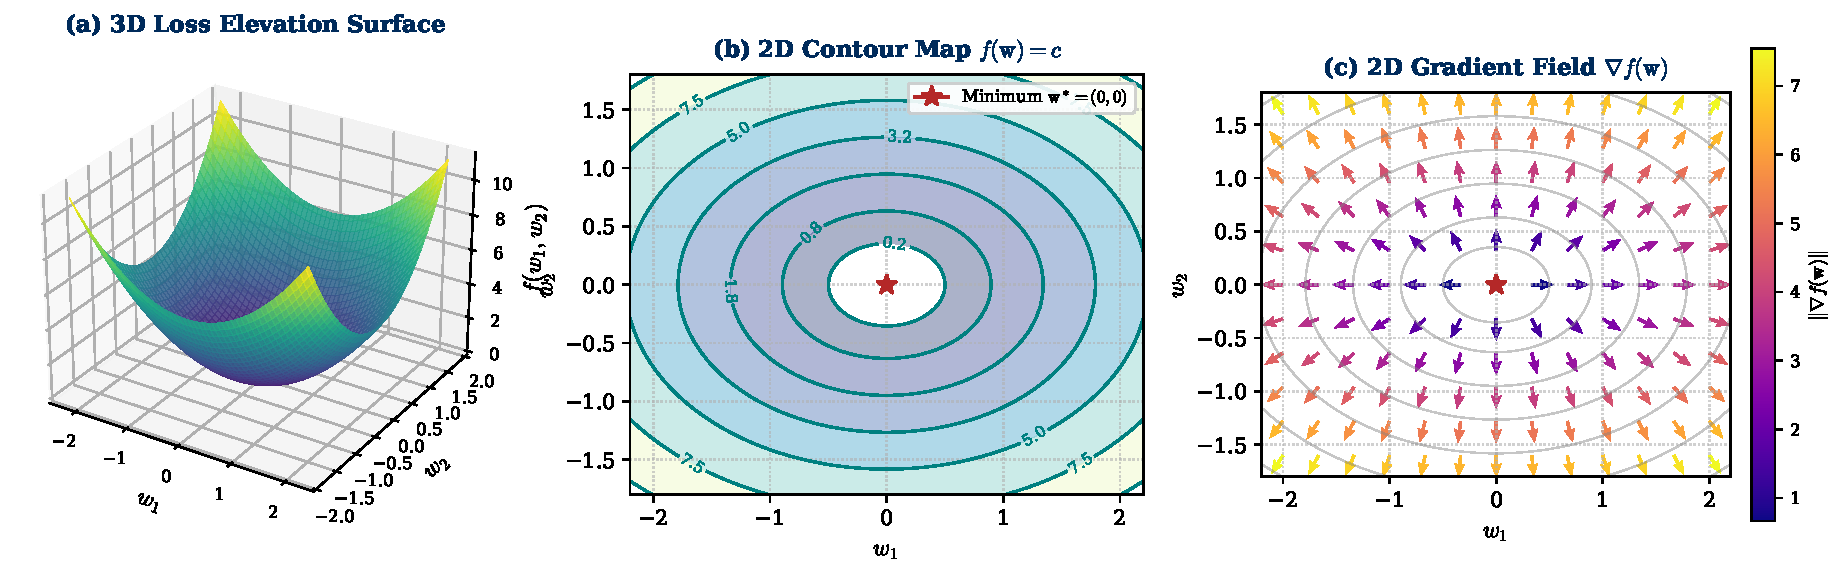
\includegraphics[width=\linewidth]{figures/gd_landscape_3panels.pdf}
\caption{Three synchronized representations of an optimization landscape $f(x, y)$: (Left) 3D surface plot displaying elevation peaks, valleys, and saddle regions; (Middle) 2D contour map showing level curves $f(x, y) = c$, where concentric closed loops enclose local minima or maxima; (Right) 2D vector field of gradients, where vector lengths indicate slope magnitude and arrows point in the direction of steepest ascent.}
\label{fig:gd_landscape_3panels}
\end{figure}

As displayed in Figure~\ref{fig:gd_landscape_3panels}:
\begin{enumerate}
  \item \textbf{3D Surface Plot (Elevation)}: Directly graphs the scalar cost value $z = f(x, y)$ as a function of the two parameters. Elevation reflects loss magnitude; global and local minima correspond to valleys.
  \item \textbf{2D Contour Map (Level Curves)}: Slices the 3D surface horizontally at constant loss elevations $f(x, y) = c$. Concentric closed isocurves enclose local extrema (minima or maxima). Spacing between contour lines indicates steepness: densely packed contours signify precipitous cliffs, whereas widely spaced contours indicate flat plateaus.
  \item \textbf{2D Gradient Vector Field}: Maps every coordinate $(x, y)$ to its gradient vector $\nabla f(x, y) = [\frac{\partial f}{\partial x}, \frac{\partial f}{\partial y}]^\top$. The arrows point in the direction of maximum instantaneous ascent, and their lengths represent the magnitude of the slope $\|\nabla f\|$.
\end{enumerate}

\subsection{Mathematical foundations: Differentiability and level curve orthogonality}
\label{sec:differentiability_and_orthogonality}

Before executing gradient updates, we must formalize two foundational mathematical principles emphasized in the AML curriculum:

\paragraph{The Differentiability Condition: Partial derivatives vs. true differentiability.}
Gradient descent updates require the objective function $f: \R^d \to \R$ to be differentiable. A frequent trap in mathematical analysis and oral examinations is confusing the existence of partial derivatives with true differentiability:
\begin{examinsight}[Oral Exam Pitfall: Differentiability vs. Partial Derivatives]
\textbf{The existence of all partial derivatives (or even all directional derivatives) does NOT imply that a function is differentiable!}\\
A multivariable function $f: \R^d \to \R$ is differentiable at $\mathbf{x}_0$ if and only if there exists a linear map (the gradient $\nabla f(\mathbf{x}_0)$) such that:
\begin{equation}
\lim_{\mathbf{h} \to \mathbf{0}} \frac{f(\mathbf{x}_0 + \mathbf{h}) - f(\mathbf{x}_0) - \nabla f(\mathbf{x}_0)^\top \mathbf{h}}{\|\mathbf{h}\|_2} = 0.
\label{eq:frechet_differentiability}
\end{equation}
By the Total Differential Theorem, a sufficient condition for differentiability is that all partial derivatives exist and are \textbf{continuous} ($f \in C^1$). If partial derivatives exist but are discontinuous, the function may fail to be differentiable, causing gradient descent to fail.
\end{examinsight}

To understand this distinction concretely, consider the classic counterexample:
\begin{equation}
f(x, y) = \begin{cases} 0 & \text{at } (x, y) = (0, 0), \\ \dfrac{x^2 y}{x^2 + y^2} & \text{elsewhere}. \end{cases}
\label{eq:differentiability_counterexample}
\end{equation}

\begin{figure}[H]
\centering
\begin{minipage}{0.48\linewidth}
  \centering
  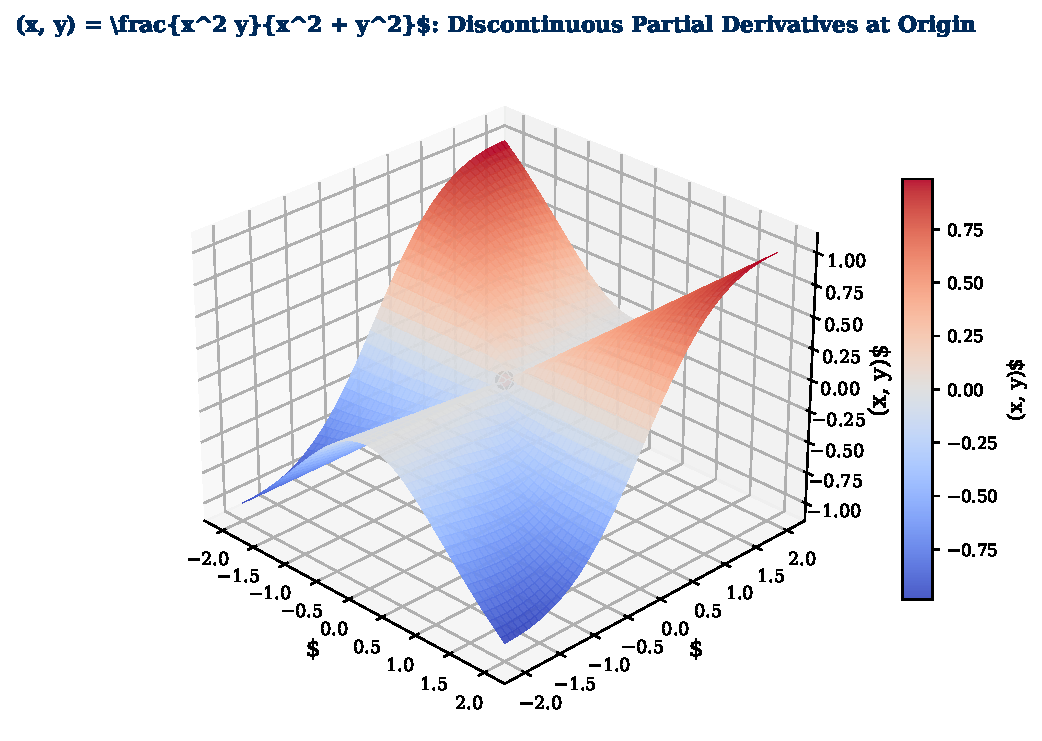
\includegraphics[width=0.95\linewidth]{figures/differentiability_counterexample_3d.pdf}
  \caption{3D surface plot of the counterexample function $f(x, y) = \frac{x^2 y}{x^2 + y^2}$ around the origin. Although partial derivatives exist everywhere, they are discontinuous at $(0, 0)$, rendering the surface non-differentiable.}
  \label{fig:differentiability_counterexample_3d}
\end{minipage}\hfill
\begin{minipage}{0.48\linewidth}
  \centering
  \begin{tikzpicture}[>=Stealth, scale=0.72, every node/.style={transform shape}]
    % Concentric elliptical contours of f(x,y)
    \draw[thick, gray!50] (0,0) ellipse (0.8cm and 0.5cm);
    \node[font=\tiny, gray!70] at (0, 0.6) {$f=0.5$};

    \draw[thick, deepdiveTeal!60] (0,0) ellipse (1.6cm and 1.0cm);
    \node[font=\tiny, deepdiveTeal!80] at (0, 1.15) {$f=1.5$};

    \draw[very thick, politoNavy] (0,0) ellipse (2.6cm and 1.6cm);
    \node[font=\scriptsize\bfseries, politoNavy] at (0, 1.8) {$\mathcal{C}_c: f(\mathbf{w}) = 2.5$};

    \draw[thick, gray!50] (0,0) ellipse (3.6cm and 2.2cm);
    \node[font=\tiny, gray!70] at (0, 2.4) {$f=4.0$};

    \draw[thick, gray!40] (0,0) ellipse (4.6cm and 2.8cm);
    \node[font=\tiny, gray!60] at (0, 3.0) {$f=6.0$};

    % Center minimum
    \fill[examred] (0,0) circle (2.5pt);
    \node[below=2pt, font=\scriptsize\bfseries, text=examred] at (0,0) {$\mathbf{w}^*$};

    % Marked point on level curve
    \coordinate (P) at (1.99, 1.03);
    \fill[politoNavy] (P) circle (3pt);
    \node[below left=2pt, font=\footnotesize\bfseries, text=politoNavy] at (P) {$\mathbf{w}_0$};

    % Tangent space line
    \draw[thick, dashed, gray!80] ($(P) + (1.61, -1.19)$) -- ($(P) + (-2.01, 1.48)$)
      node[above left, font=\scriptsize\bfseries, text=gray!90] {$\mathcal{T}_{\mathbf{w}_0}$};

    % Tangent vector v arrow
    \draw[->, very thick, deepdiveTeal] (P) -- ($(P) + (-1.21, 0.89)$)
      node[above, font=\footnotesize\bfseries, text=deepdiveTeal] {$\mathbf{v}$ ($df = 0$)};

    % Gradient vector: normal to tangent
    \draw[->, line width=1.6pt, examred] (P) -- ($(P) + (1.07, 1.45)$)
      node[above right, font=\footnotesize\bfseries, text=examred, align=left] {$\nabla f(\mathbf{w}_0)$};

    % Downhill negative gradient arrow
    \draw[->, line width=1.6pt, intuitiongreen] (P) -- ($(P) + (-1.07, -1.45)$)
      node[below right, font=\footnotesize\bfseries, text=intuitiongreen, align=left] {$-\nabla f(\mathbf{w}_0)$};

    % Right angle symbol
    \coordinate (RA1) at ($(P) + 0.28*(-0.805, 0.593)$);
    \coordinate (RA2) at ($(P) + 0.28*(-0.805, 0.593) + 0.28*(0.593, 0.805)$);
    \coordinate (RA3) at ($(P) + 0.28*(0.593, 0.805)$);
    \draw[thick, examred] (RA1) -- (RA2) -- (RA3);

    % Theorem callout
    \node[draw=politoNavy!70, fill=white, rounded corners=3pt, inner sep=3pt, font=\tiny, align=left] at (-1.8, -1.9) {
      $\langle \nabla f(\mathbf{w}_0), \mathbf{v} \rangle = 0 \quad \forall \mathbf{v} \in \mathcal{T}_{\mathbf{w}_0}$\\
      $\implies \nabla f \perp \text{Level Curves}$
    };
  \end{tikzpicture}
  \caption{Geometric orthogonality of the gradient to contour level curves. Along the isocurve $f(x, y) = 2.5$, the directional derivative along any tangent vector $\mathbf{v}$ is zero ($\langle \nabla f, \mathbf{v} \rangle = 0$). The negative gradient $-\nabla f$ points strictly perpendicular to the level curve in the direction of steepest descent.}
  \label{fig:gradient_orthogonal_level_curves}
\end{minipage}
\end{figure}

Evaluating the partial derivatives of Equation~\eqref{eq:differentiability_counterexample} at the coordinate origin via the difference quotient:
\begin{align}
\frac{\partial f}{\partial x}(0, 0) &= \lim_{h \to 0} \frac{f(h, 0) - f(0, 0)}{h} = \lim_{h \to 0} \frac{0 - 0}{h} = 0, \\
\frac{\partial f}{\partial y}(0, 0) &= \lim_{h \to 0} \frac{f(0, h) - f(0, 0)}{h} = \lim_{h \to 0} \frac{0 - 0}{h} = 0.
\end{align}
Both partial derivatives exist and equal zero at the origin. However, computing the partial derivative with respect to $y$ along the line $y = 0$ for any $x \ne 0$:
\begin{equation}
\frac{\partial f}{\partial y}(x, 0) = \left. \frac{x^2(x^2 + y^2) - x^2 y(2y)}{(x^2 + y^2)^2} \right|_{y=0} = \frac{x^4}{x^4} = 1.
\end{equation}
Meanwhile, along the $y$-axis ($x = 0$): $\frac{\partial f}{\partial y}(0, y) = 0$. Therefore, $\lim_{(x, y) \to (0, 0)} \frac{\partial f}{\partial y}(x, y)$ does not exist! The partial derivative is \textbf{discontinuous at the origin}, proving that $f(x, y)$ is not differentiable at $(0, 0)$, despite all directional derivatives being well-defined.

\paragraph{Orthogonality of the gradient to level curves.}
A second foundational geometric theorem is that the gradient vector is strictly \textbf{orthogonal} to the contour level curves (or level hypersurfaces in higher dimensions).

Let $\mathcal{C}_c \triangleq \{ \mathbf{w} \in \R^d : f(\mathbf{w}) = c \}$ be an isocurve of constant value $c$. Let $\mathbf{r}(t)$ be an arbitrary smooth path lying entirely within the level set, such that $f(\mathbf{r}(t)) = c$ for all $t$. Differentiating both sides with respect to scalar parameter $t$ via the multivariate chain rule:
\begin{equation}
\frac{d}{dt} f(\mathbf{r}(t)) = \nabla f(\mathbf{r}(t))^\top \mathbf{r}'(t) = 0.
\label{eq:level_curve_orthogonality_proof}
\end{equation}
Here, $\mathbf{r}'(t) \equiv \mathbf{v}$ is the tangent velocity vector along the contour curve. Equation~\eqref{eq:level_curve_orthogonality_proof} proves that:
\begin{equation}
\langle \nabla f(\mathbf{w}), \mathbf{v} \rangle = 0 \quad \text{for any tangent vector } \mathbf{v} \text{ to the isocurve}.
\end{equation}
Because the inner product vanishes, the directional derivative along the isocurve is zero: moving tangentially to a level set produces zero instantaneous change in loss. 

Conversely, the direction perpendicular to the tangent space maximizes the inner product, proving that the gradient vector $\nabla f(\mathbf{w})$ is \textbf{perpendicular to the level curves}, pointing toward steepest ascent, while the negative gradient $-\nabla f(\mathbf{w})$ points perpendicular to the level curves toward steepest descent (as illustrated in Figure~\ref{fig:gradient_orthogonal_level_curves}).

\subsection{Stationary points and initialization sensitivity}
\label{sec:stationary_points_initialization}

A point $\mathbf{x}^* \in \R^d$ where the gradient vanishes identically is defined as a \textbf{stationary point} (or critical point):
\begin{equation}
\nabla f(\mathbf{x}^*) = \mathbf{0}.
\label{eq:stationary_point_def}
\end{equation}
Evaluating the gradient descent update rule at a stationary point reveals an immediate consequence:
\begin{equation}
\mathbf{x}^{(t+1)} = \mathbf{x}^{(t)} - \alpha \nabla f(\mathbf{x}^{(t)}) = \mathbf{x}^{(t)} - \mathbf{0} = \mathbf{x}^{(t)}.
\end{equation}
Standard first-order gradient descent \textbf{gets stuck} at any stationary point, terminating all parameter updates.

However, a fundamental distinction must be drawn:
\begin{equation}
\text{Stationary Point } (\nabla f = \mathbf{0}) \quad \not\implies \quad \text{Local Minimum!}
\end{equation}
A stationary point can be a local minimum, a local maximum, or a saddle point. 

\begin{figure}[H]
\centering
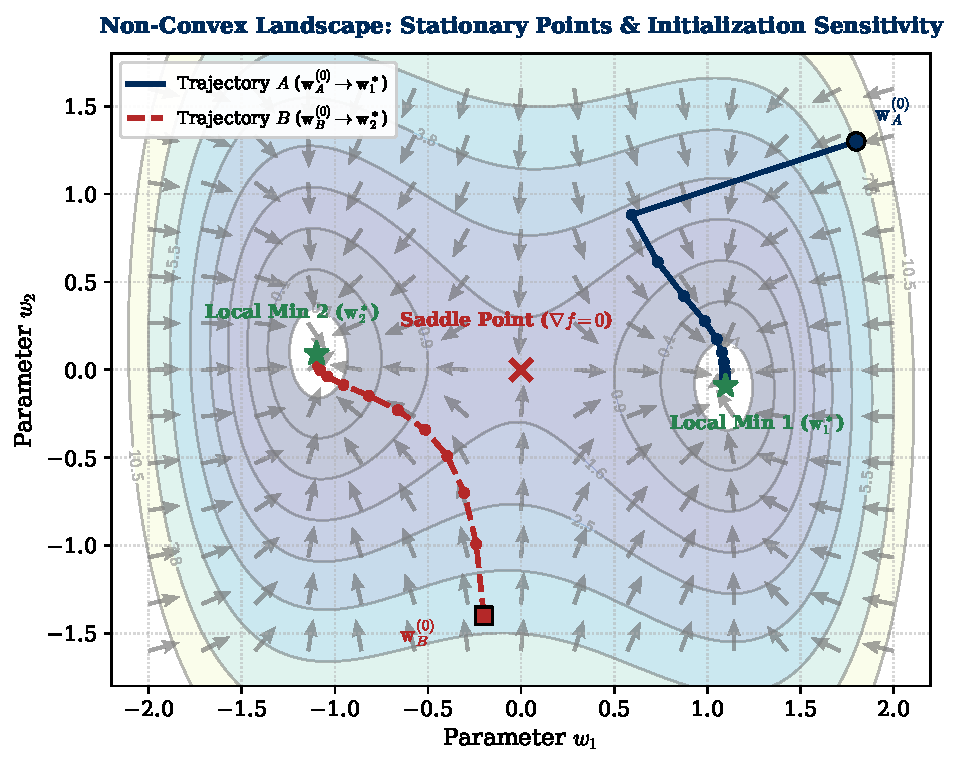
\includegraphics[width=0.55\linewidth]{figures/gd_trajectories_initialization.pdf}
\caption{Optimization trajectories on a non-convex vector field from different parameter initializations. Starting from the upper-right point, gradient updates follow the negative gradient arrows directly into a local minimum basin. Starting from the lower-left point, updates diverge along a completely different path toward a saddle region or alternative basin.}
\label{fig:gd_trajectories_initialization}
\end{figure}

As visualized in Figure~\ref{fig:gd_trajectories_initialization}, which stationary point gradient descent reaches depends entirely on the initial parameter configuration $\mathbf{x}^{(0)}$. In complex non-convex landscapes, different initializations lead to vastly different local basins or saddle geometries.

\subsection{Directional derivative and the proof of steepest descent}
\label{sec:directional_derivative_proof}

To formalize gradient descent from first principles, we analyze how a multivariate function changes along arbitrary spatial trajectories.

Let $f: \R^d \to \R$ be continuously differentiable ($C^1$). Let $\mathbf{u} \in \R^d$ be an arbitrary unit direction vector ($\|\mathbf{u}\|_2 = 1$). The \textbf{directional derivative} of $f$ at point $\mathbf{w}$ along direction $\mathbf{u}$ is defined as the limit:
\begin{equation}
D_\mathbf{u} f(\mathbf{w}) = \lim_{\epsilon \to 0} \frac{f(\mathbf{w} + \epsilon \mathbf{u}) - f(\mathbf{w})}{\epsilon}.
\label{eq:directional_derivative_def}
\end{equation}
By multivariable Taylor theorem, expanding $f(\mathbf{w} + \epsilon \mathbf{u})$ around $\mathbf{w}$:
\begin{equation}
f(\mathbf{w} + \epsilon \mathbf{u}) = f(\mathbf{w}) + \epsilon \nabla f(\mathbf{w})^\top \mathbf{u} + \mathcal{O}(\epsilon^2).
\end{equation}
Substituting this expansion into Equation~\eqref{eq:directional_derivative_def}:
\begin{equation}
D_\mathbf{u} f(\mathbf{w}) = \lim_{\epsilon \to 0} \frac{\epsilon \nabla f(\mathbf{w})^\top \mathbf{u} + \mathcal{O}(\epsilon^2)}{\epsilon} = \nabla f(\mathbf{w})^\top \mathbf{u}.
\label{eq:directional_derivative_inner_product}
\end{equation}
The rate of change along direction $\mathbf{u}$ is given by the inner product of the gradient vector $\nabla f(\mathbf{w})$ with $\mathbf{u}$.

To minimize $f(\mathbf{w})$, we seek the unit direction $\mathbf{u}^*$ that minimizes the directional derivative (i.e., maximizes the rate of instantaneous decrease):
\begin{equation}
\mathbf{u}^* = \arg\min_{\|\mathbf{u}\|_2 = 1} D_\mathbf{u} f(\mathbf{w}) = \arg\min_{\|\mathbf{u}\|_2 = 1} \nabla f(\mathbf{w})^\top \mathbf{u}.
\label{eq:steepest_descent_problem}
\end{equation}
By the Cauchy-Schwarz inequality, for any two vectors $\mathbf{a}, \mathbf{b} \in \R^d$:
\begin{equation}
|\mathbf{a}^\top \mathbf{b}| \le \|\mathbf{a}\|_2 \|\mathbf{b}\|_2 \implies -\sum_{j=1}^d a_j b_j \ge -\|\mathbf{a}\|_2 \|\mathbf{b}\|_2.
\end{equation}
Applying this bound to Equation~\eqref{eq:steepest_descent_problem} with $\mathbf{a} = \nabla f(\mathbf{w})$ and $\mathbf{b} = \mathbf{u}$ (where $\|\mathbf{u}\|_2 = 1$):
\begin{equation}
\nabla f(\mathbf{w})^\top \mathbf{u} \ge -\|\nabla f(\mathbf{w})\|_2 \|\mathbf{u}\|_2 = -\|\nabla f(\mathbf{w})\|_2.
\label{eq:cauchy_schwarz_lower_bound}
\end{equation}
Equality holds if and only if vector $\mathbf{u}$ is collinear with $\nabla f(\mathbf{w})$ and points in the opposite direction:
\begin{equation}
\mathbf{u}^* = -\frac{\nabla f(\mathbf{w})}{\|\nabla f(\mathbf{w})\|_2}.
\label{eq:steepest_descent_direction}
\end{equation}
This rigorous derivation proves Cauchy's 1847 theorem~\cite{cauchy1847methode}: \textbf{the negative gradient direction $-\nabla f(\mathbf{w})$ is the direction of steepest instantaneous descent}.

Geometrically, because $\nabla f(\mathbf{w})$ is strictly perpendicular to the level curves of a continuous surface, stepping along $-\nabla f(\mathbf{w})$ guarantees maximum loss reduction per unit distance moved in high-dimensional spaces.

\subsection{First-order Taylor expansion and the gradient descent update}
\label{sec:first_order_taylor}

We parameterize a finite step of length $\eta > 0$ along direction $\mathbf{u}^*$, yielding displacement $\Delta \mathbf{w} = -\eta \nabla f(\mathbf{w})$. The first-order Taylor series approximation around point $\mathbf{w}_t$ is:
\begin{equation}
f(\mathbf{w}_t - \eta \nabla f(\mathbf{w}_t)) \approx f(\mathbf{w}_t) - \eta \|\nabla f(\mathbf{w}_t)\|_2^2 + \mathcal{O}(\eta^2).
\label{eq:taylor_first_order}
\end{equation}
Because $\|\nabla f(\mathbf{w}_t)\|_2^2 > 0$ for any non-stationary point, there exists a sufficiently small step size $\eta > 0$ such that the second-order remainder is dominated by the linear decrease:
\begin{equation}
f(\mathbf{w}_t - \eta \nabla f(\mathbf{w}_t)) < f(\mathbf{w}_t).
\end{equation}
This establishes the classical \textbf{Gradient Descent update rule}:
\begin{equation}
\mathbf{w}_{t+1} = \mathbf{w}_t - \eta \nabla f(\mathbf{w}_t),
\label{eq:gradient_descent_update}
\end{equation}
where $\eta > 0$ is the \textbf{learning rate} (step size hyperparameter).

\subsection{Learning rate dynamics: Under-stepping vs. divergence}
\label{sec:learning_rate_dynamics}

The magnitude of the learning rate $\eta$ critically dictates optimization stability:

\begin{figure}[H]
\centering
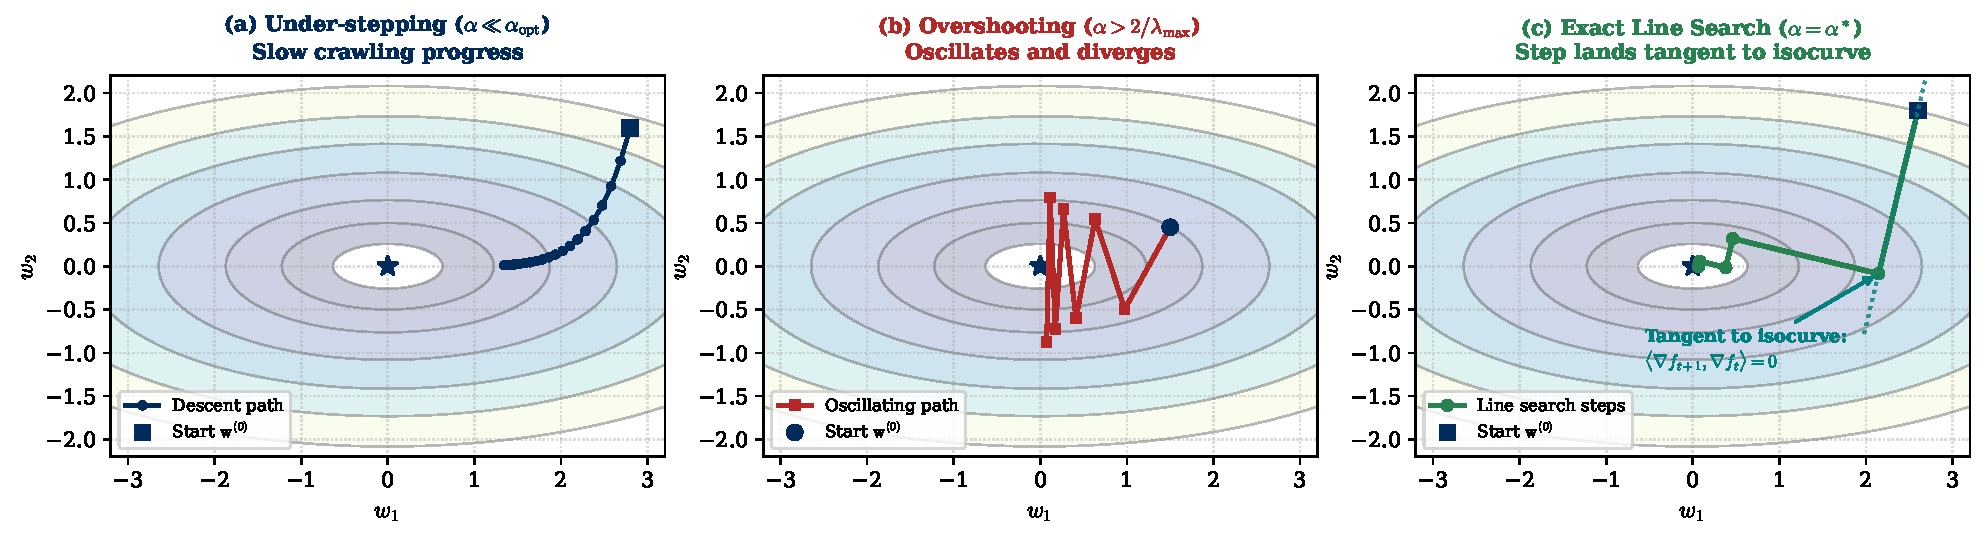
\includegraphics[width=\linewidth]{figures/learning_rate_dynamics_contours.pdf}
\caption{Contour dynamics of gradient descent under varying step sizes $\alpha$: (Left) An excessively small learning rate causes crawling, agonizingly slow progress along the contour gradient; (Middle) An excessively large learning rate overshoots the minimum, oscillating across valley walls with increasing amplitude and ultimately diverging; (Right) An optimal step size determined via line search $\arg\min_\alpha f(\mathbf{x}^{(t)} - \alpha \nabla f(\mathbf{x}^{(t)}))$, where each update lands precisely where the descent direction is tangent to a contour isocurve.}
\label{fig:slide_learning_rates}
\end{figure}

As illustrated across the contour landscapes in Figure~\ref{fig:slide_learning_rates}:
\begin{itemize}
  \item \textbf{Effective Step Length}: An essential mathematical nuance is that the geometric length of the parameter update is not simply the scalar learning rate $\alpha$, but rather the norm-scaled quantity $\alpha \|\nabla f(\mathbf{x}^{(t)})\|$. In regions where the gradient is steep, the parameter displacement is proportionally magnified; conversely, on shallow plateaus where $\|\nabla f\| \approx 0$, progress stalls regardless of $\alpha$.
  \item \textbf{Under-stepping ($\alpha \to 0$)}: When $\alpha$ is excessively conservative, parameter updates $\Delta \mathbf{x}^{(t)}$ are microscopic. Iterations advance imperceptibly, requiring thousands of steps to cross moderate distances and rendering the optimizer vulnerable to premature convergence on deceptive plateaus.
  \item \textbf{Overshooting and Divergence ($\alpha \gg \alpha_{\text{crit}}$)}: When $\alpha$ exceeds the critical threshold dictated by the maximum eigenvalue of the Hessian ($\alpha > 2/\lambda_{\max}$, proven in Section~\ref{sec:condition_number_ravines}), the first-order Taylor approximation breaks down completely. Updates violently oscillate back and forth between opposing valley walls with geometrically increasing amplitude, driving objective values toward infinity: $\lim_{t \to \infty} f(\mathbf{x}^{(t)}) = \infty$.
  \item \textbf{Optimal Step Size via Exact Line Search}: In classical optimization, the optimal step size is determined adaptively by solving a one-dimensional sub-problem along the negative gradient ray:
    \begin{equation}
    \alpha^* = \arg\min_{\alpha > 0} f\left(\mathbf{x}^{(t)} - \alpha \nabla f(\mathbf{x}^{(t)})\right).
    \label{eq:exact_line_search}
    \end{equation}
    Evaluating the optimality condition by differentiating with respect to $\alpha$ via the multivariate chain rule:
    \begin{equation}
    \frac{d}{d\alpha} f\left(\mathbf{x}^{(t)} - \alpha \nabla f(\mathbf{x}^{(t)})\right) = -\nabla f\left(\mathbf{x}^{(t+1)}\right)^\top \nabla f\left(\mathbf{x}^{(t)}\right) = 0.
    \label{eq:line_search_orthogonality}
    \end{equation}
    Equation~\eqref{eq:line_search_orthogonality} reveals a fundamental geometric theorem: at the exact line-search minimizer, the new gradient $\nabla f(\mathbf{x}^{(t+1)})$ is strictly perpendicular to the previous search direction $-\nabla f(\mathbf{x}^{(t)})$. In terms of contour topology, this means the gradient direction at the landing point is \textbf{tangent to the local isocurve} (level set), producing the characteristic orthogonal zig-zag trajectory shown in the right panel of Figure~\ref{fig:slide_learning_rates}.
\end{itemize}

\subsection{Learning rate decay schedules: Linear, inverse, and exponential}
\label{sec:learning_rate_decay_schedules}

Fixing a constant scalar learning rate $\alpha$ forces an undesirable trade-off: a large learning rate enables rapid traversal of distant plateaus early in training but prevents convergence near the minimum due to endless cross-valley oscillations; conversely, a small learning rate ensures stable fine-grained convergence but crawls agonizingly slowly at initialization.

To reconcile these competing objectives, the learning rate can be modulated dynamically over iterations according to a deterministic \textbf{decay schedule} parameterized by a decay factor $\rho > 0$:

\paragraph{Linear decay schedule.}
The linear decay schedule interpolates parameter updates uniformly from an initial step size $\alpha^{(0)}$ down to a designated final floor $\alpha^{(\rho)}$ over a budget of $\rho$ iterations:
\begin{equation}
\alpha^{(t+1)} = \left(1 - \frac{t}{\rho}\right)\alpha^{(0)} + \frac{t}{\rho}\alpha^{(\rho)}, \quad \text{for } 0 \le t \le \rho.
\label{eq:linear_decay_schedule}
\end{equation}
At iteration $t = 0$, $\alpha^{(1)} = \alpha^{(0)}$. At the terminal horizon $t = \rho$, the learning rate contracts precisely to $\alpha^{(\rho)}$ (typically chosen orders of magnitude smaller than $\alpha^{(0)}$). For iterations $t > \rho$, the rate remains fixed at $\alpha^{(\rho)}$. This schedule provides predictable, constant-rate deceleration.

\paragraph{Inverse decay schedule (Time-based decay).}
The inverse decay schedule attenuates the step size inversely with the elapsed iteration count:
\begin{equation}
\alpha^{(t+1)} = \frac{\alpha^{(t)}}{1 + \rho t}.
\label{eq:inverse_decay_schedule}
\end{equation}
In its direct non-recursive formulation, $\alpha^{(t)} = \frac{\alpha^{(0)}}{1 + \rho t}$. This schedule enforces an asymptotic decay rate of $\mathcal{O}(1/t)$, mirroring the classical Robbins-Monro stochastic convergence rate (detailed in Section~\ref{sec:robbins_monro}) while ensuring rapid initial dampening that smoothly transitions into a long-tailed fine-tuning regime.

\paragraph{Exponential decay schedule.}
The exponential decay schedule applies continuous geometric dampening scaled by decay rate $\rho > 0$:
\begin{equation}
\alpha^{(t+1)} = \alpha^{(0)} e^{-\rho t}.
\label{eq:exponential_decay_schedule}
\end{equation}
Because the step size contracts by a constant multiplicative factor $e^{-\rho}$ at every iteration, exponential decay rapidly quenches parameter updates. In contemporary deep learning practice, this is frequently discretized into \emph{step decay} (e.g., decaying $\alpha$ by a factor of $0.1$ or $0.2$ every fixed number of epochs).

Although first-order gradient descent guarantees monotonic cost reduction on smooth surfaces when the step size is sufficiently small, its foundational premise---that the objective function is well-approximated by a flat tangent hyperplane---breaks down on realistic optimization surfaces. When a loss landscape features high anisotropic curvature, such as elongated ravines where the slope across the walls is orders of magnitude steeper than along the floor, gradient descent exhibits pathological cross-valley bouncing and stalls completely. To diagnose and transcend these geometric limitations, we must incorporate second-order curvature information encoded by the Hessian matrix, as developed in Section~\ref{sec:second_order_curvature}.

\section{Second-order curvature, the Hessian matrix, and ill-conditioned ravines}
\label{sec:second_order_curvature}

First-order optimization methods navigate loss landscapes solely on the basis of instantaneous slope, assuming that local descent directions remain reliable over finite distances. However, real-world objective surfaces are curved, undulating, and non-isotropic. The rate at which the gradient itself varies across parameter space---quantified by second-order partial derivatives---critically determines whether an update step successfully descends toward a minimum or violently overshoots into divergence.

The most notorious impediment to first-order optimization is the geometry of \textbf{ill-conditioned ravines}: long, narrow valleys flanked by steep canyon walls and possessing a gently sloping floor. In such landscapes, the curvature across the valley walls dwarfs the curvature along the valley base. Because gradient descent updates are constrained by the maximum curvature to prevent explosive divergence across the walls, parameter updates along the gentle floor crawl at a glacial, near-imperceptible pace. The optimizer spends nearly all its computational effort oscillating perpendicularly between opposing walls rather than advancing toward the true minimizer.

This section develops the mathematical framework of second-order optimization and curvature analysis. We begin by formulating the Hessian matrix and the second-order Taylor expansion, proving how its eigenvalues dictate directional curvature. We then contrast the isotropic quadratic surrogate minimized by first-order gradient descent with the true osculating quadratic model minimized by the Newton-Raphson method, illustrating their distinct step behaviors via native geometric schematics. Finally, we formalize the Hessian condition number $\kappa$, derive the exact upper bound on the stable learning rate $\eta < 2/\lambda_{\max}$, and demonstrate why extreme condition numbers induce catastrophic oscillations in standard gradient descent.

\subsection{The Hessian matrix and second-order Taylor expansion}
\label{sec:hessian_matrix}

Let $f: \R^d \to \R$ be twice continuously differentiable ($C^2$). The second-order Taylor series approximation of $f$ around point $\mathbf{w}$ for an arbitrary displacement $\Delta \mathbf{w} \in \R^d$ is:
\begin{equation}
f(\mathbf{w} + \Delta \mathbf{w}) \approx f(\mathbf{w}) + \nabla f(\mathbf{w})^\top \Delta \mathbf{w} + \frac{1}{2} \Delta \mathbf{w}^\top \mathbf{H}(\mathbf{w}) \Delta \mathbf{w},
\label{eq:second_order_taylor}
\end{equation}
where $\mathbf{H}(\mathbf{w}) \in \R^{d \times d}$ is the \textbf{Hessian matrix} of second-order partial derivatives:
\begin{equation}
\mathbf{H}_{jk}(\mathbf{w}) = \frac{\partial^2 f(\mathbf{w})}{\partial w_j \partial w_k}, \quad j, k \in \{1, \dots, d\}.
\label{eq:hessian_def}
\end{equation}
By Schwarz's theorem on the equality of mixed partials, $\frac{\partial^2 f}{\partial w_j \partial w_k} = \frac{\partial^2 f}{\partial w_k \partial w_j}$, guaranteeing that $\mathbf{H}$ is a real symmetric matrix ($\mathbf{H} = \mathbf{H}^\top$).

By the spectral theorem, the symmetric Hessian admits an orthogonal eigendecomposition:
\begin{equation}
\mathbf{H} = \mathbf{Q} \mathbf{\Lambda} \mathbf{Q}^\top = \sum_{i=1}^d \lambda_i \mathbf{q}_i \mathbf{q}_i^\top,
\label{eq:hessian_spectral}
\end{equation}
where $\mathbf{Q} = [\mathbf{q}_1, \dots, \mathbf{q}_d] \in \R^{d \times d}$ is an orthonormal matrix of eigenvectors ($\mathbf{q}_i^\top \mathbf{q}_j = \delta_{ij}$), and $\mathbf{\Lambda} = \operatorname{diag}(\lambda_1, \dots, \lambda_d)$ contains real eigenvalues ordered such that $\lambda_{\max} \equiv \lambda_1 \ge \lambda_2 \ge \dots \ge \lambda_d \equiv \lambda_{\min}$.

The quadratic term $\frac{1}{2} \Delta \mathbf{w}^\top \mathbf{H} \Delta \mathbf{w}$ characterizes directional curvature:
\begin{itemize}[noitemsep]
  \item If $\Delta \mathbf{w}$ aligns with eigenvector $\mathbf{q}_i$, the second-order change is $\frac{1}{2} \lambda_i \|\Delta \mathbf{w}\|_2^2$.
  \item A positive eigenvalue ($\lambda_i > 0$) signifies positive curvature (the function curves upward like a bowl).
  \item A negative eigenvalue ($\lambda_i < 0$) signifies negative curvature (the function curves downward like a dome).
  \item A zero eigenvalue ($\lambda_i = 0$) signifies flat curvature (the function is locally linear along $\mathbf{q}_i$).
\end{itemize}

\paragraph{Optimal step size under second-order curvature.}
Substituting the gradient descent step $\Delta \mathbf{w} = -\eta \mathbf{g}$ (where $\mathbf{g} = \nabla f(\mathbf{w})$) into Equation~\eqref{eq:second_order_taylor}:
\begin{equation}
f(\mathbf{w} - \eta \mathbf{g}) \approx f(\mathbf{w}) - \eta \mathbf{g}^\top \mathbf{g} + \frac{1}{2} \eta^2 \mathbf{g}^\top \mathbf{H} \mathbf{g}.
\label{eq:gd_step_taylor2}
\end{equation}
To find the step size $\eta^*$ that maximizes expected decrease, we differentiate Equation~\eqref{eq:gd_step_taylor2} with respect to scalar $\eta$ and set the derivative to zero:
\begin{equation}
\frac{d}{d\eta} \left[ f(\mathbf{w}) - \eta \|\mathbf{g}\|_2^2 + \frac{1}{2} \eta^2 \mathbf{g}^\top \mathbf{H} \mathbf{g} \right] = -\|\mathbf{g}\|_2^2 + \eta \mathbf{g}^\top \mathbf{H} \mathbf{g} = 0 \implies \eta^* = \frac{\mathbf{g}^\top \mathbf{g}}{\mathbf{g}^\top \mathbf{H} \mathbf{g}}.
\label{eq:optimal_eta_hessian}
\end{equation}
If the gradient vector happens to align with the dominant eigenvector of the Hessian ($\mathbf{g} \approx \mathbf{q}_1$), the optimal learning rate contracts to $\eta^* = 1/\lambda_{\max}$. Moreover, convergence requires:
\begin{equation}
0 < \eta < \frac{2}{\lambda_{\max}(\mathbf{H})}.
\label{eq:learning_rate_stability_bound}
\end{equation}
If $\eta \ge 2/\lambda_{\max}$, the quadratic term exceeds the linear decrease, and the iterates diverge.

\subsection{Second-order optimization: Newton-Raphson vs. Gradient Descent surrogates}
\label{sec:newton_vs_gd_surrogates}

To comprehend the fundamental divergence between first-order and second-order optimization, we examine the implicit local surrogate models that guide their respective update steps.

At each iteration $\vw$, first-order gradient descent with step size $\eta$ implicitly minimizes a first-order Taylor expansion regularized by an isotropic proximal penalty:
\begin{equation}
\Delta \vw_{\text{GD}} = \argmin_{\Delta \vw} \left[ f(\vw) + \nabla f(\vw)^\top \Delta \vw + \frac{1}{2\eta} \|\Delta \vw\|_2^2 \right] = -\eta \nabla f(\vw).
\label{eq:gd_quadratic_surrogate}
\end{equation}
Geometrically, Equation~\eqref{eq:gd_quadratic_surrogate} models the loss landscape as an \textbf{isotropic spherical bowl} with uniform curvature $1/\eta$ along all spatial directions. The optimizer completely ignores directional variation in terrain steepness, stepping strictly in the direction of steepest instantaneous ascent without regard to whether the slope curves sharply upward or flattens out.

In sharp contrast, the classical multivariate \textbf{Newton-Raphson method} minimizes the \textbf{true osculating second-order Taylor expansion}:
\begin{equation}
q_{\text{Newton}}(\Delta \vw) = f(\vw) + \nabla f(\vw)^\top \Delta \vw + \frac{1}{2} \Delta \vw^\top \mathbf{H}(\vw) \Delta \vw.
\label{eq:newton_taylor_model}
\end{equation}
Assuming the Hessian $\mathbf{H}(\vw)$ is positive definite ($\mathbf{H} \succ 0$), setting the gradient of the surrogate to zero yields:
\begin{equation}
\nabla_{\Delta \vw} q_{\text{Newton}}(\Delta \vw) = \nabla f(\vw) + \mathbf{H}(\vw) \Delta \vw = \mathbf{0} \implies \Delta \vw_{\text{Newton}} = -[\mathbf{H}(\vw)]^{-1} \nabla f(\vw).
\label{eq:newton_step_derivation}
\end{equation}
The Newton-Raphson parameter update is therefore:
\begin{equation}
\vw_{t+1} = \vw_t - [\mathbf{H}(\vw_t)]^{-1} \nabla f(\vw_t).
\label{eq:newton_update_rule}
\end{equation}

\begin{figure}[H]
\centering
\begin{minipage}{0.48\linewidth}
  \centering
  \begin{tikzpicture}[scale=0.82]
    % 1D Surrogate Comparison
    \draw[-{Stealth[length=2mm]}, thick, gray!70] (-0.3, 0) -- (6.0, 0) node[right, font=\scriptsize] {$w$};
    \draw[-{Stealth[length=2mm]}, thick, gray!70] (0, -0.3) -- (0, 4.5) node[above, font=\scriptsize] {Loss};
    \node[font=\bfseries\sffamily, text=politoNavy] at (3.0, 4.3) {(a) 1D Local Quadratic Surrogates};

    % True objective f(w) = 0.2*(x-3.8)^2 + 0.08*(x-3.8)^3 + 0.6
    \draw[very thick, politoNavy, domain=0.4:5.4, samples=80] plot (\x, {0.2*(\x-3.8)^2 + 0.08*(\x-3.8)^3 + 0.6});
    \node[font=\scriptsize\bfseries, text=politoNavy] at (5.2, 1.6) {$f(w)$};

    % Current point w_t at x = 1.2
    \coordinate (wt) at (1.2, {0.2*(1.2-3.8)^2 + 0.08*(1.2-3.8)^3 + 0.6});
    \fill[black] (wt) circle (2.2pt);
    \node[above left=1pt, font=\scriptsize\bfseries] at (wt) {$w_t$};

    % First-order tangent line
    \draw[thick, dashed, gray!60, domain=0.4:3.0] plot (\x, {1.8 + (-0.95)*(\x-1.2)});
    \node[font=\tiny, text=gray!80, rotate=-42] at (2.2, 0.65) {Tangent Plane};

    % GD surrogate (isotropic bowl with scalar step)
    \draw[thick, dashed, examred, domain=0.5:3.2, samples=60] plot (\x, {1.8 - 0.95*(\x-1.2) + 0.9*(\x-1.2)^2});
    \fill[examred] (1.73, 0) circle (1.8pt) node[below, font=\scriptsize\bfseries, text=examred] {$w_{\text{GD}}$};
    \draw[dotted, examred] (1.73, 0) -- (1.73, 1.3);

    % Newton surrogate (exact osculating quadratic)
    \draw[thick, intuitiongreen, domain=0.8:5.2, samples=60] plot (\x, {1.8 - 0.95*(\x-1.2) + 0.18*(\x-1.2)^2});
    \fill[intuitiongreen] (3.84, 0) circle (1.8pt) node[below, font=\scriptsize\bfseries, text=intuitiongreen] {$w_{\text{Newton}}$};
    \draw[dotted, intuitiongreen] (3.84, 0) -- (3.84, 0.55);

    \node[font=\tiny, align=left, text=examred] at (1.1, 3.2) {GD Surrogate $q_{\text{GD}}$\\(Isotropic bowl $\frac{1}{2\eta}(w-w_t)^2$)};
    \node[font=\tiny, align=left, text=intuitiongreen] at (4.5, 3.2) {Newton Surrogate $q_{\text{Newton}}$\\(Osculating $\frac{1}{2}H(w-w_t)^2$)};
  \end{tikzpicture}
\end{minipage}\hfill
\begin{minipage}{0.48\linewidth}
  \centering
  \begin{tikzpicture}[scale=0.82]
    % 2D Step Direction on Anisotropic Contours
    \draw[-{Stealth[length=2mm]}, thick, gray!60] (-3.4, 0) -- (3.6, 0) node[right, font=\scriptsize] {$w_1$ (Gentle base)};
    \draw[-{Stealth[length=2mm]}, thick, gray!60] (0, -2.2) -- (0, 2.4) node[above, font=\scriptsize] {$w_2$ (Steep wall)};
    \node[font=\bfseries\sffamily, text=politoNavy] at (0, 2.6) {(b) Anisotropic Elliptical Contours};

    % Elliptical level curves centered at origin (0, 0)
    \draw[politoNavy!30, thick] (0, 0) ellipse (3.1 and 1.5);
    \draw[politoNavy!50, thick] (0, 0) ellipse (2.3 and 1.05);
    \draw[politoNavy!70, thick] (0, 0) ellipse (1.5 and 0.65);
    \draw[politoNavy!90, thick] (0, 0) ellipse (0.7 and 0.28);

    % Optimum
    \node[star, star points=5, star point ratio=2.2, fill=intuitiongreen, inner sep=1.8pt] at (0, 0) {};
    \node[below left=1pt, font=\scriptsize\bfseries, text=intuitiongreen] at (0, 0) {$\mathbf{w}^*$};

    % Starting point w_0
    \coordinate (w0) at (2.4, 1.15);
    \fill[black] (w0) circle (2.2pt);
    \node[above right, font=\scriptsize\bfseries] at (w0) {$\mathbf{w}_0$};

    % GD Step: perpendicular to level curve (steepest descent)
    \draw[-{Stealth[length=2.5mm]}, very thick, examred] (w0) -- ($(w0) + (-0.6, -1.25)$) 
      node[below right, font=\scriptsize\bfseries, text=examred, align=left] {GD Step $-\eta \nabla f$\\(Orthogonal to contour)};
    \draw[dotted, thick, examred] ($(w0) + (-0.6, -1.25)$) -- ($(w0) + (-1.1, 0.1)$) -- ($(w0) + (-1.5, -0.7)$);

    % Newton Step: directly to minimum!
    \draw[-{Stealth[length=2.5mm]}, very thick, intuitiongreen] (w0) -- (0, 0)
      node[pos=0.45, above right, font=\scriptsize\bfseries, text=intuitiongreen, align=left] {Newton Step $-\mathbf{H}^{-1}\nabla f$\\(Points straight to $\mathbf{w}^*$)};
  \end{tikzpicture}
\end{minipage}
\caption{Geometric comparison between first-order Gradient Descent and second-order Newton-Raphson optimization. (a) In one dimension, gradient descent implicitly constructs an isotropic quadratic surrogate with fixed artificial curvature $1/\eta$, yielding small incremental steps; Newton-Raphson constructs the true osculating quadratic model matching local Hessian curvature, leaping directly to the surrogate minimum. (b) On anisotropic elliptical contours ($\kappa \gg 1$), the negative gradient $-\nabla f$ is strictly perpendicular to level curves, directing updates into steep valley walls and causing oscillatory zig-zags; the inverse Hessian $\mathbf{H}^{-1}$ rescales and rotates coordinates by inverse directional curvatures, guiding the Newton step straight to the global minimizer $\mathbf{w}^*$ in a single leap on quadratic surfaces.}
\label{fig:newton_vs_gd_surrogates}
\end{figure}

\begin{intuition}[Spectral Action of the Inverse Hessian]
To understand how Newton's method eliminates ill-conditioning, express the step in the orthonormal eigenbasis of the Hessian $\mathbf{H} = \mathbf{Q} \mathbf{\Lambda} \mathbf{Q}^\top$. Rotating coordinate displacements to $\Delta \tilde{\vw} = \mathbf{Q}^\top \Delta \vw$ and gradients to $\tilde{\mathbf{g}} = \mathbf{Q}^\top \nabla f(\vw)$:
\begin{equation}
\Delta \tilde{\vw}_{\text{Newton}} = -\mathbf{\Lambda}^{-1} \tilde{\mathbf{g}} = -\begin{bmatrix} \tilde{g}_1 / \lambda_1 \\ \tilde{g}_2 / \lambda_2 \\ \vdots \\ \tilde{g}_d / \lambda_d \end{bmatrix}.
\label{eq:newton_eigenspace_action}
\end{equation}
Equation~\eqref{eq:newton_eigenspace_action} demonstrates the profound auto-adaptive scaling of second-order optimization:
\begin{itemize}[noitemsep]
  \item Along directions of high curvature ($\lambda_i = \lambda_{\max} \gg 0$), the step is aggressively dampened by $1/\lambda_{\max}$, eliminating cross-ravine overshooting.
  \item Along directions of low curvature ($\lambda_i = \lambda_{\min} \approx 0$), the step is massively amplified by $1/\lambda_{\min}$, accelerating rapidly along the flat valley base.
\end{itemize}
If the objective function is purely quadratic, Newton's method reaches the exact minimizer in a \textbf{single step} ($\vw_1 = \vw^*$), rendering convergence speed completely invariant to the condition number $\kappa$!
\end{intuition}

\subsection{The condition number and ill-conditioned ravines}
\label{sec:condition_number_ravines}

A fundamental computational bottleneck for first-order gradient descent is the phenomenon of \textbf{ill-conditioned ravines} (also known as valleys or canyons).

\begin{definition}[Hessian condition number]
For a convex objective with positive definite Hessian ($\mathbf{H} \succ 0$, so all $\lambda_i > 0$), the \textbf{condition number} $\kappa \ge 1$ is defined as the ratio of maximum to minimum eigenvalue:
\begin{equation}
\kappa(\mathbf{H}) = \frac{\lambda_{\max}(\mathbf{H})}{\lambda_{\min}(\mathbf{H})}.
\label{eq:condition_number_def}
\end{equation}
\end{definition}

When $\kappa \approx 1$, the contour lines of the loss surface are isotropic hyperspheres. The gradient vector points directly toward the minimum, and gradient descent converges rapidly.

However, when $\kappa \gg 1$ (e.g., $\kappa = 10^3$ or $10^5$), the problem is termed \textbf{ill-conditioned}. The contour lines form elongated, highly eccentric ellipsoids.

\begin{figure}[H]
\centering
\begin{minipage}{0.48\linewidth}
  \centering
  \begin{tikzpicture}[scale=0.68, every node/.style={transform shape}]
    % Axes
    \draw[-{Stealth}, gray!60, thick] (-3.8, 0) -- (4.0, 0) node[right, font=\footnotesize] {$\mathbf{q}_2$ ($\lambda_{\min}$)};
    \draw[-{Stealth}, gray!60, thick] (0, -2.0) -- (0, 2.0) node[above, font=\footnotesize] {$\mathbf{q}_1$ ($\lambda_{\max}$)};

    % Contours
    \draw[politoNavy!35, thick] (0, 0) ellipse (3.5 and 1.6);
    \draw[politoNavy!55, thick] (0, 0) ellipse (2.7 and 1.15);
    \draw[politoNavy!75, thick] (0, 0) ellipse (1.9 and 0.75);
    \draw[politoNavy!90, thick] (0, 0) ellipse (1.2 and 0.4);
    \draw[politoNavy, thick] (0, 0) ellipse (0.5 and 0.15);

    % Minimizer
    \node[star, star points=5, star point ratio=2.25, fill=intuitiongreen, inner sep=2pt, label={below left:\scriptsize $\mathbf{w}^*$}] at (0, 0) {};

    % Trajectory
    \coordinate (p0) at (3.1, 1.35);
    \coordinate (p1) at (2.8, -1.05);
    \coordinate (p2) at (2.5, 0.82);
    \coordinate (p3) at (2.2, -0.62);
    \coordinate (p4) at (1.9, 0.48);
    \coordinate (p5) at (1.6, -0.35);
    \coordinate (p6) at (1.3, 0.25);

    \draw[-{Stealth}, thick, examred] (p0) -- (p1);
    \draw[-{Stealth}, thick, examred] (p1) -- (p2);
    \draw[-{Stealth}, thick, examred] (p2) -- (p3);
    \draw[-{Stealth}, thick, examred] (p3) -- (p4);
    \draw[-{Stealth}, thick, examred] (p4) -- (p5);
    \draw[-{Stealth}, thick, examred] (p5) -- (p6);

    \foreach \p in {p0,p1,p2,p3,p4,p5,p6} {
      \fill[examred] (\p) circle (1.6pt);
    }
    \node[above right, font=\scriptsize\bfseries, text=examred] at (p0) {$\mathbf{w}_0$};

    \node[font=\scriptsize, text=examred, align=center] at (2.2, -1.6) {Cross-ravine\\oscillations};
    \node[font=\scriptsize, text=deepdiveTeal, align=center] at (-1.8, 1.2) {Slow progress\\along base};
  \end{tikzpicture}
\end{minipage}\hfill
\begin{minipage}{0.48\linewidth}
  \centering
  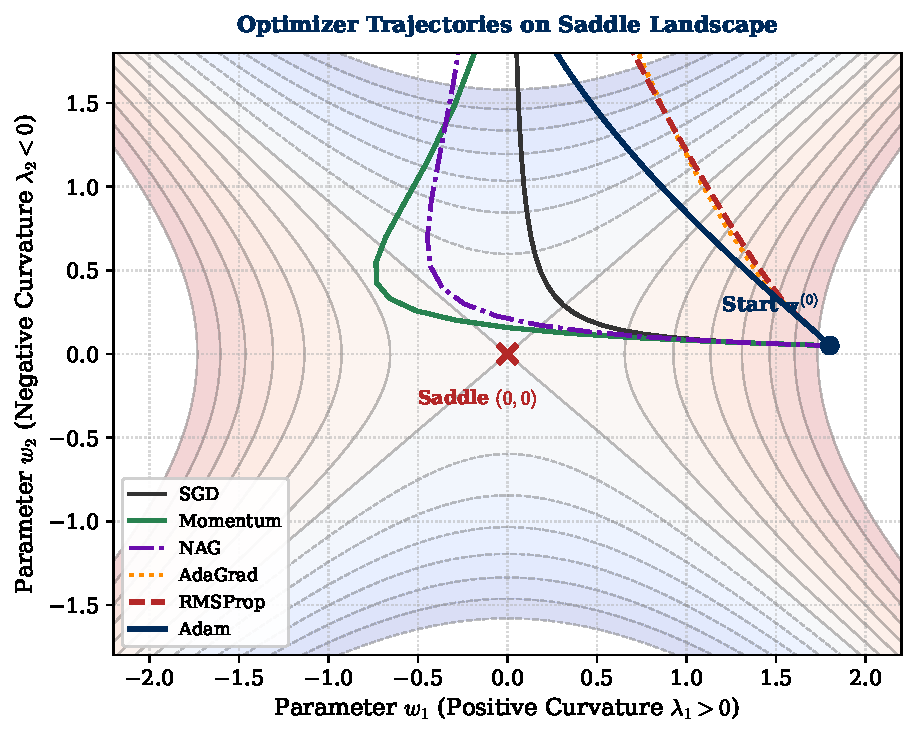
\includegraphics[width=\linewidth]{figures/cs231n_optimizer_comparison.pdf}
\end{minipage}
\caption{Optimization dynamics in ill-conditioned ravines and complex landscapes. Left: Native vector representation of an ill-conditioned quadratic valley ($\kappa = \lambda_{\max}/\lambda_{\min} \gg 1$), where first-order gradient descent oscillates violently across the steep walls along $\mathbf{q}_1$ while making negligible progress along the flat base $\mathbf{q}_2$. Right: Benchmark comparison across optimizers (SGD, Momentum, NAG, AdaGrad, AdaDelta, RMSProp) traversing a saddle topology, demonstrating how momentum and adaptive learning rates overcome anisotropic curvature.}
\label{fig:slide_ill_conditioned_ravine}
\end{figure}

As visualized in Figure~\ref{fig:slide_ill_conditioned_ravine}:
\begin{itemize}
  \item Along the direction of maximum curvature $\mathbf{q}_1$ (across the ravine walls), the loss changes rapidly with eigenvalue $\lambda_{\max}$.
  \item Along the direction of minimum curvature $\mathbf{q}_2$ (along the ravine base leading to the minimum), the loss changes extremely slowly with eigenvalue $\lambda_{\min}$.
  \item The stability bound in Equation~\eqref{eq:learning_rate_stability_bound} restricts the global learning rate to $\eta < 2/\lambda_{\max}$.
  \item Because $\eta$ must be chosen small to prevent explosive divergence across the steep walls, progress along the flat base is scaled by $\eta \lambda_{\min} < 2 \frac{\lambda_{\min}}{\lambda_{\max}} = \frac{2}{\kappa} \ll 1$.
\end{itemize}
Consequently, first-order gradient descent oscillates violently back and forth between the opposing walls of the ravine, making negligible forward progress toward the true minimizer.

While Newton-Raphson optimization elegantly eliminates ill-conditioning by rotating and rescaling the descent trajectory via the inverse Hessian matrix, its practical application to modern neural networks is thwarted by an insurmountable computational barrier. Computing the full $d \times d$ Hessian requires evaluating second-order derivatives across millions to billions of parameters, demanding prohibitive memory storage ($\mathcal{O}(d^2)$) and an impossible cubic inversion cost ($\mathcal{O}(d^3)$ arithmetic operations per step). Machine learning practitioners are thus confronted with a critical imperative: how can an optimizer overcome cross-ravine oscillations and accelerate along the gentle base of ill-conditioned valleys using \textit{only first-order gradient evaluations}? This fundamental question leads directly to Polyak's classical momentum and the lineage of adaptive first-order optimizers developed in Section~\ref{sec:first_order_acceleration_methods}.

\section{First-order acceleration methods: Momentum and unified matrix scaling}
\label{sec:first_order_acceleration_methods}

In high-dimensional non-convex optimization, standard first-order gradient descent behaves like a memoryless physical system: at every iteration, the parameter vector acts as an idealized massless particle that instantly resets its velocity to match the instantaneous negative gradient. While this reactive behavior works satisfactorily on perfectly isotropic quadratic surfaces, it fails catastrophically in the presence of anisotropic curvature and ill-conditioned ravines ($\kappa \gg 1$). In such geometries, the optimizer is buffeted back and forth between opposing valley walls, dissipating nearly all its computational energy in high-frequency cross-valley oscillations while making negligible longitudinal progress toward the minimum.

To overcome this fundamental limitation without incurring the prohibitive $\mathcal{O}(d^3)$ cost of explicit second-order Hessian inversion, statistical learning turns to the principles of classical mechanics. By imbuing the optimizer with \textbf{physical momentum}, the parameter vector is modeled not as a massless point, but as a heavy marble rolling down a frictioned potential well. Historical gradient vectors are accumulated into an internal velocity state, allowing persistent directional forces along the valley floor to build up constructive kinetic energy while high-frequency cross-ravine gradient oscillations cancel each other out destructively.

This section systematically constructs the theory of first-order acceleration methods. We begin with Polyak's classical momentum formulation, detailing its physical velocity accumulation and oscillation-dampening mechanisms. We then derive the exact asymptotic terminal velocity on persistent slopes, proving the celebrated $1/(1-\lambda)$ acceleration factor. Next, we unroll the recursive optimization dynamics to expose standard gradient descent as uniform historical weighting and momentum as an exponentially decayed memory filter. Finally, we formulate the unified diagonal scaling matrix framework $\boldsymbol{\Gamma}_i^t$, revealing how AdaGrad, RMSprop, and Adam adaptively scale step sizes across individual coordinates to conquer disparate curvatures.

\subsection{Classical momentum: Velocity accumulation and oscillation dampening}
\label{sec:classical_momentum}

The classical momentum method, formulated by Boris Polyak in 1964~\cite{polyak1964some}, draws direct inspiration from physical mechanics. Rather than treating the parameter vector as a massless particle whose velocity instantly matches the local negative gradient, the optimizer models a heavy marble rolling down a frictioned potential well.

The algorithm introduces an internal state vector $\mathbf{v}^{(t)} \in \R^d$, termed the \textbf{velocity}, and updates parameters according to the coupled recurrence:
\begin{align}
\mathbf{v}^{(t+1)} &= \lambda \mathbf{v}^{(t)} - \alpha \nabla f(\mathbf{x}^{(t)}), \label{eq:momentum_velocity_update} \\
\mathbf{x}^{(t+1)} &= \mathbf{x}^{(t)} + \mathbf{v}^{(t+1)}, \label{eq:momentum_position_update}
\end{align}
where $\alpha > 0$ is the learning rate, and $\lambda \in [0, 1)$ is the \textbf{momentum coefficient} (or friction parameter, typically set to $\lambda = 0.9$ or $0.99$).

\paragraph{Physical mechanism in ill-conditioned valleys.}
When $\lambda = 0$, the velocity simplifies to $\mathbf{v}^{(t+1)} = -\alpha \nabla f(\mathbf{x}^{(t)})$, collapsing immediately to standard gradient descent. 
When $\lambda > 0$, the velocity retains an exponential moving average of historical gradient directions:
\begin{itemize}[noitemsep]
  \item \textbf{Transverse cross-ravine direction ($\mathbf{q}_1$)}: Because the optimizer repeatedly bounces back and forth across the opposing valley walls, the signs of consecutive partial derivatives alternate: $\nabla f(\mathbf{x}^{(t)})_{\mathbf{q}_1} \approx -\nabla f(\mathbf{x}^{(t-1)})_{\mathbf{q}_1}$. In the velocity accumulator of Equation~\eqref{eq:momentum_velocity_update}, these opposing vectors cancel out destructively:
  \begin{equation}
  \mathbf{v}^{(t+1)}_{\mathbf{q}_1} \approx \lambda \mathbf{v}^{(t)}_{\mathbf{q}_1} - \alpha \nabla f(\mathbf{x}^{(t)})_{\mathbf{q}_1} \approx \mathbf{0}.
  \end{equation}
  This destructive interference aggressively dampens high-frequency cross-ravine oscillations.
  \item \textbf{Longitudinal base direction ($\mathbf{q}_2$)}: Along the gentle descent floor of the valley leading toward the minimizer, consecutive gradients point consistently in the same downhill direction: $\nabla f(\mathbf{x}^{(t)})_{\mathbf{q}_2} \approx \nabla f(\mathbf{x}^{(t-1)})_{\mathbf{q}_2}$. Here, the historical velocity terms add constructively, accumulating directional speed along the base.
\end{itemize}

\subsection{Effective terminal step length and aligned gradient acceleration}
\label{sec:aligned_gradient_acceleration}

A central pedagogical result is quantifying the exact acceleration gain when gradients are persistently aligned.

Suppose the optimizer traverses a uniform slope where the gradient remains constant over consecutive iterations: $\nabla f(\mathbf{x}^{(t)}) \approx \mathbf{g}$. Assuming initial velocity $\mathbf{v}^{(0)} = \mathbf{0}$, unrolling the recurrence in Equation~\eqref{eq:momentum_velocity_update} yields:
\begin{align}
\mathbf{v}^{(1)} &= -\alpha \mathbf{g}, \nonumber \\
\mathbf{v}^{(2)} &= -\lambda \alpha \mathbf{g} - \alpha \mathbf{g} = -\alpha (1 + \lambda) \mathbf{g}, \nonumber \\
\mathbf{v}^{(3)} &= -\lambda \alpha (1 + \lambda) \mathbf{g} - \alpha \mathbf{g} = -\alpha (1 + \lambda + \lambda^2) \mathbf{g}, \nonumber \\
&\;\;\vdots \nonumber \\
\mathbf{v}^{(t+1)} &= -\alpha \mathbf{g} \sum_{k=0}^t \lambda^k.
\label{eq:momentum_geometric_series}
\end{align}
Because $\lambda \in [0, 1)$, the finite summation in Equation~\eqref{eq:momentum_geometric_series} is a geometric progression. Taking the limit as $t \to \infty$:
\begin{equation}
\lim_{t \to \infty} \sum_{k=0}^t \lambda^k = \frac{1}{1 - \lambda}.
\end{equation}
Consequently, the terminal velocity and effective parameter displacement per step converge to:
\begin{equation}
\lim_{t \to \infty} \|\mathbf{v}^{(t+1)}\| = \frac{1}{1 - \lambda} \alpha \|\mathbf{g}\| = \frac{1}{1 - \lambda} \alpha \|\nabla f\|.
\label{eq:terminal_momentum_step}
\end{equation}
Equation~\eqref{eq:terminal_momentum_step} reveals the remarkable speedup factor of momentum:
\begin{itemize}[noitemsep]
  \item For standard gradient descent, the step length along a flat plateau with gradient $\|\nabla f\|$ is strictly $\alpha \|\nabla f\|$.
  \item For momentum with $\lambda = 0.9$, the effective step length expands to $\frac{1}{1 - 0.9}\alpha \|\nabla f\| = \mathbf{10 \alpha \|\nabla f\|}$ ($10\times$ acceleration).
  \item For momentum with $\lambda = 0.99$, the effective step length expands to $\frac{1}{1 - 0.99}\alpha \|\nabla f\| = \mathbf{100 \alpha \|\nabla f\|}$ ($100\times$ acceleration).
\end{itemize}
This dynamic amplification enables momentum to surge rapidly through flat regions and provides the kinetic energy required to carry parameter updates over shallow local barriers into deeper, more generalizing minima basins.

\subsection{Mathematical unrolling: Standard gradient descent vs. momentum}
\label{sec:unrolling_gd_momentum}

To understand how momentum transforms optimization trajectories over an entire training run, we analyze the concept of \textbf{unrolling the optimization recurrence}.

\paragraph{Unrolling standard gradient descent.}
For standard gradient descent without momentum, parameter updates follow $\mathbf{x}^{(t+1)} = \mathbf{x}^{(t)} - \alpha \nabla f(\mathbf{x}^{(t)})$. Unrolling step by step from initialization $\mathbf{x}^{(0)}$:
\begin{align}
\mathbf{x}^{(1)} &= \mathbf{x}^{(0)} - \alpha \nabla f(\mathbf{x}^{(0)}), \nonumber \\
\mathbf{x}^{(2)} &= \mathbf{x}^{(1)} - \alpha \nabla f(\mathbf{x}^{(1)}) = \mathbf{x}^{(0)} - \alpha \nabla f(\mathbf{x}^{(0)}) - \alpha \nabla f(\mathbf{x}^{(1)}), \nonumber \\
&\;\;\vdots \nonumber \\
\mathbf{x}^{(t+1)} &= \mathbf{x}^{(0)} - \alpha \sum_{i=1}^t \nabla f(\mathbf{x}^{(i)}).
\label{eq:unrolled_gd}
\end{align}
Equation~\eqref{eq:unrolled_gd} shows that in standard gradient descent, the net parameter displacement $\mathbf{x}^{(t+1)} - \mathbf{x}^{(0)}$ is simply the unweighted sum of all historical gradients, multiplied by constant step size $-\alpha$. Every historical gradient receives identical weighting, regardless of whether it was computed at the start of training or in the current iteration.

\paragraph{Unrolling gradient descent with momentum.}
Now consider the momentum update defined by Equations~\eqref{eq:momentum_velocity_update}--\eqref{eq:momentum_position_update}. Assuming $\mathbf{v}^{(0)} = \mathbf{0}$, the velocity at any iteration $k \ge 1$ is an exponentially decayed sum of past gradients:
\begin{equation}
\mathbf{v}^{(k)} = -\alpha \sum_{j=1}^k \lambda^{k-j} \nabla f(\mathbf{x}^{(j-1)}).
\end{equation}
Since $\mathbf{x}^{(t+1)} = \mathbf{x}^{(0)} + \sum_{k=1}^{t+1} \mathbf{v}^{(k)}$, the cumulative displacement after $t+1$ steps is:
\begin{equation}
\mathbf{x}^{(t+1)} = \mathbf{x}^{(0)} - \alpha \sum_{k=1}^{t+1} \sum_{j=1}^k \lambda^{k-j} \nabla f(\mathbf{x}^{(j-1)}).
\end{equation}
To determine the net coefficient multiplying each individual gradient $\nabla f(\mathbf{x}^{(i)})$ (for $i = 1, \dots, t$), we observe how often $\nabla f(\mathbf{x}^{(i)})$ enters into subsequent velocity terms:
\begin{itemize}[noitemsep]
  \item At iteration $k = i+1$, $\nabla f(\mathbf{x}^{(i)})$ enters with weight $-\alpha \lambda^0 = -\alpha$.
  \item At iteration $k = i+2$, it persists decayed by $-\alpha \lambda^1$.
  \item At iteration $k = i+3$, it persists decayed by $-\alpha \lambda^2$.
  \item $\dots$
  \item At iteration $k = t+1$, it persists decayed by $-\alpha \lambda^{t-i}$.
\end{itemize}
Summing these contributions across all subsequent steps gives a finite geometric series of length $t - i + 1$:
\begin{equation}
\sum_{m=0}^{t-i} \lambda^m = \frac{1 - \lambda^{t-i+1}}{1 - \lambda} = \frac{1 - \lambda^{t+1-i}}{1 - \lambda}.
\end{equation}
Substituting this closed-form coefficient into the unrolled parameter position yields the exact momentum unrolling formula:
\begin{equation}
\mathbf{x}^{(t+1)} = \mathbf{x}^{(0)} - \alpha \sum_{i=1}^t \left( \frac{1 - \lambda^{t+1-i}}{1 - \lambda} \right) \nabla f(\mathbf{x}^{(i)}).
\label{eq:unrolled_momentum}
\end{equation}
For early gradients where $t - i \gg 0$, $\lambda^{t+1-i} \to 0$, so their cumulative weight saturates at $-\frac{\alpha}{1 - \lambda}$. For very recent gradients ($i \approx t$), the weight is approximately $-\alpha$. This provides a smooth, recency-weighted memory filter over the optimization trajectory.

\subsection{Unified diagonal scaling matrix framework: Unifying AdaGrad, RMSprop, and Adam}
\label{sec:unified_diagonal_scaling}

The unrolled formulations of Equations~\eqref{eq:unrolled_gd} and~\eqref{eq:unrolled_momentum} represent special cases of a far more general algebraic structure. Any first-order optimization method can be expressed in the \textbf{unified unrolled form}:
\begin{equation}
\mathbf{x}^{(t+1)} = \mathbf{x}^{(0)} - \alpha \sum_{i=1}^t \boldsymbol{\Gamma}_i^t \nabla f(\mathbf{x}^{(i)}),
\label{eq:unified_scaling_matrix}
\end{equation}
where $\boldsymbol{\Gamma}_i^t \in \R^{d \times d}$ is a time-varying \textbf{diagonal scaling matrix}:
\begin{equation}
\boldsymbol{\Gamma}_i^t = \operatorname{diag}\left( \gamma_{i, 1}^t, \, \gamma_{i, 2}^t, \, \dots, \, \gamma_{i, d}^t \right).
\end{equation}

This formulation highlights a profound architectural insight behind Equation~\eqref{eq:unified_scaling_matrix}: standard momentum applies a single scalar coefficient to all coordinates simultaneously. However, in complex high-dimensional architectures, different parameters experience drastically different gradient magnitudes and curvatures. The diagonal scaling matrix $\boldsymbol{\Gamma}_i^t$ enables the optimizer to assign coordinate-specific acceleration strengths and adaptive step sizes along each individual coordinate direction.

This unified matrix formulation elegantly subsumes the entire lineage of modern deep learning optimizers:
\begin{enumerate}
  \item \textbf{Standard Gradient Descent}: $\boldsymbol{\Gamma}_i^t = \mathbf{I}$, assigning uniform isotropic scalar weighting across all coordinates.
  \item \textbf{Classical Momentum}: $\boldsymbol{\Gamma}_i^t = \left(\frac{1 - \lambda^{t+1-i}}{1 - \lambda}\right)\mathbf{I}$, assigning identical exponentially accumulated scalar weights to all coordinates.
  \item \textbf{AdaGrad (Adaptive Gradient Algorithm)}~\cite{duchi2011adaptive}: Accumulates historical squared gradients per coordinate: $G_{t, jj} = \sum_{k=1}^t (\nabla f(\mathbf{x}^{(k)}))_j^2$. The scaling entries are set to:
    \begin{equation}
    \gamma_{i, j}^t \propto \frac{1}{\sqrt{G_{t, jj} + \epsilon}}.
    \end{equation}
    Coordinates with historically frequent or steep gradients are dampened, while coordinates with rare or small gradients receive larger relative steps.
  \item \textbf{RMSprop (Root Mean Square Propagation)}~\cite{goodfellow2016deep}: Resolves AdaGrad's premature learning rate collapse by replacing monotonic sum $G_t$ with an exponentially decaying moving average of squared gradients:
    \begin{equation}
    v_{t, j} = \beta v_{t-1, j} + (1 - \beta) (\nabla f(\mathbf{x}^{(t)}))_j^2, \quad \gamma_{i, j}^t \propto \frac{1}{\sqrt{v_{t, j} + \epsilon}}.
    \end{equation}
  \item \textbf{Adam (Adaptive Moment Estimation)}~\cite{kingma2014adam}: Combines both principles simultaneously: it computes first-moment momentum tracking in the numerator (velocity accumulation) and second-moment uncentered variance tracking in the denominator (RMSprop scaling), with bias-correction factors to compensate for zero-initialization. In the unrolled view of Equation~\eqref{eq:unified_scaling_matrix}, Adam corresponds to a fully adaptive diagonal matrix $\boldsymbol{\Gamma}_i^t$ that dynamically re-scales each parameter coordinate based on its individual signal-to-noise ratio.
\end{enumerate}

Although momentum and adaptive diagonal scaling provide powerful mechanisms for traversing ill-conditioned valleys and accelerating through flat regions, they were originally conceived within the paradigm of convex or locally unimodal optimization. Deep neural architectures, however, present a radically more complex challenge: the composition of multi-layer nonlinear transformations shatters convexity completely, creating high-dimensional loss landscapes populated by astronomically many critical points---including local minima, local maxima, and complex saddle surfaces. Furthermore, simply locating an empirical minimum does not ensure predictive success, as different minima exhibit wildly divergent generalization properties on unseen data. To optimize deep models effectively, we must therefore investigate the topology of critical points and the delicate interplay between curvature and generalization, as explored in Section~\ref{sec:critical_points_deep_learning}.

\section{Critical points and optimization in deep learning: Generalization vs. global minima}
\label{sec:critical_points_deep_learning}

In classical convex optimization, the landscape of the objective function is inherently benign: every stationary point where the gradient vanishes is guaranteed to be a global minimum, ensuring that local search trajectories converge to globally optimal parameters regardless of initialization. In deep neural networks, however, permutation symmetries among hidden units and the cascaded nesting of non-linear activations shatter convexity completely. The resulting parameter space is characterized by an intricate, non-convex terrain punctuated by an astronomical proliferation of critical points, flat plateaus, and treacherous ravines.

For decades, the central fear in non-convex optimization was that gradient-based algorithms would become irrevocably trapped in suboptimal, high-loss local minima. However, modern high-dimensional probability and random matrix theory have revolutionized our understanding of deep loss surfaces: in millions of dimensions, the probability that all eigenvalues of the Hessian are simultaneously positive at a high loss elevation decays exponentially to zero. The primary obstacles that impede training are not isolated local minima, but rather high-index saddle points and vast degenerate plateaus. Crucially, the ultimate objective of machine learning is not to achieve the absolute lowest empirical training loss, but to identify parameter configurations that generalize robustly to unseen test distributions.

This section investigates the topology of critical points in deep learning and formalizes the geometry of generalization. We first establish the spectral classification of critical points via Hessian eigenvalues, characterizing local minima, local maxima, and saddle points. We then unpack the modern consensus dispelling the local minima myth through the theoretical insights of Dauphin et al., showing how saddle points proliferate in high dimensions. Next, we analyze the geometry of generalization by contrasting sharp minima with flat minima under distribution shift, demonstrating why wide basins prevent catastrophic generalization gaps. Finally, we establish why iterative first-order optimization remains indispensable even on strictly convex problems due to computational and numerical stability constraints.

\subsection{Classification of critical points via Hessian eigenvalues}
\label{sec:hessian_classification}

At a critical point $\mathbf{w}^*$, the linear Taylor term in Equation~\eqref{eq:second_order_taylor} vanishes, leaving the local behavior entirely governed by the quadratic form $\frac{1}{2} \Delta \mathbf{w}^\top \mathbf{H}(\mathbf{w}^*) \Delta \mathbf{w}$:
\begin{enumerate}
  \item \textbf{Local Minimum}: The Hessian is positive definite ($\mathbf{H} \succ 0$, all $\lambda_i > 0$). Any displacement strictly increases the loss: $f(\mathbf{w}^* + \Delta \mathbf{w}) > f(\mathbf{w}^*)$.
  \item \textbf{Local Maximum}: The Hessian is negative definite ($\mathbf{H} \prec 0$, all $\lambda_i < 0$). Any displacement strictly decreases the loss: $f(\mathbf{w}^* + \Delta \mathbf{w}) < f(\mathbf{w}^*)$.
  \item \textbf{Saddle Point}: The Hessian has mixed eigenvalues ($\exists \lambda_i > 0$ and $\exists \lambda_j < 0$). The function curves upward along eigenvector $\mathbf{q}_i$ and curves downward along eigenvector $\mathbf{q}_j$.
\end{enumerate}

\begin{figure}[H]
\centering
\begin{minipage}{0.48\linewidth}
  \centering
  \begin{tikzpicture}[>=Stealth, scale=0.75, every node/.style={transform shape}]
    % Axes
    \draw[->, thick, gray!80] (-3.2, 0) -- (3.2, 0) node[right, font=\tiny\bfseries, text=politoNavy] {$w_1$ ($\lambda_1 > 0$)};
    \draw[->, thick, gray!80] (0, -2.6) -- (0, 2.6) node[above, font=\tiny\bfseries, text=examred] {$w_2$ ($\lambda_2 < 0$)};

    % Inflow arrows along w1 axis (Stable manifold)
    \draw[->, very thick, politoNavy] (2.8, 0) -- (1.4, 0);
    \draw[->, very thick, politoNavy] (1.4, 0) -- (0.5, 0);
    \draw[->, very thick, politoNavy] (-2.8, 0) -- (-1.4, 0);
    \draw[->, very thick, politoNavy] (-1.4, 0) -- (-0.5, 0);

    % Outflow arrows along w2 axis (Unstable manifold)
    \draw[->, very thick, examred] (0, 0.5) -- (0, 1.4);
    \draw[->, very thick, examred] (0, 1.4) -- (0, 2.4);
    \draw[->, very thick, examred] (0, -0.5) -- (0, -1.4);
    \draw[->, very thick, examred] (0, -1.4) -- (0, -2.4);

    % Hyperbolic streamlines in quadrants
    % Quadrant 1
    \draw[thick, deepdiveTeal, domain=0.45:2.6, samples=50] plot (\x, {0.8/\x});
    \draw[->, thick, deepdiveTeal] (1.2, {0.8/1.2}) -- (1.0, {0.8/1.0});

    \draw[thick, deepdiveTeal, domain=0.8:2.8, samples=50] plot (\x, {2.0/\x});
    \draw[->, thick, deepdiveTeal] (1.8, {2.0/1.8}) -- (1.5, {2.0/1.5});

    % Quadrant 2
    \draw[thick, deepdiveTeal, domain=-2.6:-0.45, samples=50] plot (\x, {-0.8/\x});
    \draw[->, thick, deepdiveTeal] (-1.2, {-0.8/-1.2}) -- (-1.0, {-0.8/-1.0});

    \draw[thick, deepdiveTeal, domain=-2.8:-0.8, samples=50] plot (\x, {-2.0/\x});
    \draw[->, thick, deepdiveTeal] (-1.8, {-2.0/-1.8}) -- (-1.5, {-2.0/-1.5});

    % Quadrant 3
    \draw[thick, deepdiveTeal, domain=-2.6:-0.45, samples=50] plot (\x, {0.8/\x});
    \draw[->, thick, deepdiveTeal] (-1.2, {0.8/-1.2}) -- (-1.0, {0.8/-1.0});

    \draw[thick, deepdiveTeal, domain=-2.8:-0.8, samples=50] plot (\x, {2.0/\x});
    \draw[->, thick, deepdiveTeal] (-1.8, {2.0/-1.8}) -- (-1.5, {2.0/-1.5});

    % Quadrant 4
    \draw[thick, deepdiveTeal, domain=0.45:2.6, samples=50] plot (\x, {-0.8/\x});
    \draw[->, thick, deepdiveTeal] (1.2, {-0.8/1.2}) -- (1.0, {-0.8/1.0});

    \draw[thick, deepdiveTeal, domain=0.8:2.8, samples=50] plot (\x, {-2.0/\x});
    \draw[->, thick, deepdiveTeal] (1.8, {-2.0/1.8}) -- (1.5, {-2.0/1.5});

    % Critical saddle point at origin
    \fill[white] (0,0) circle (3pt);
    \draw[line width=1.3pt, examred] (-0.12, -0.12) -- (0.12, 0.12);
    \draw[line width=1.3pt, examred] (-0.12, 0.12) -- (0.12, -0.12);
    \node[below left=2pt, font=\tiny\bfseries, text=examred] at (0,0) {Saddle $\mathbf{w}^* = \mathbf{0}$};

    % Annotation callout
    \node[draw=politoNavy!70, fill=white, rounded corners=3pt, font=\tiny, align=left, inner sep=3pt] at (2.0, -1.9) {
      $f = w_1^2 - w_2^2$\\
      $\mathbf{H} = \mathrm{diag}(+2, -2)$\\
      Inflow along $w_1$\\
      Outflow along $w_2$
    };
  \end{tikzpicture}
  \caption{Vector field and contour topology around critical points, illustrating how gradients vanish ($\nabla f = \mathbf{0}$) at stationary points and distinguishing a hyperbolic saddle point from a local minimum basin.}
  \label{fig:slide_saddle_point}
\end{minipage}\hfill
\begin{minipage}{0.48\linewidth}
  \centering
  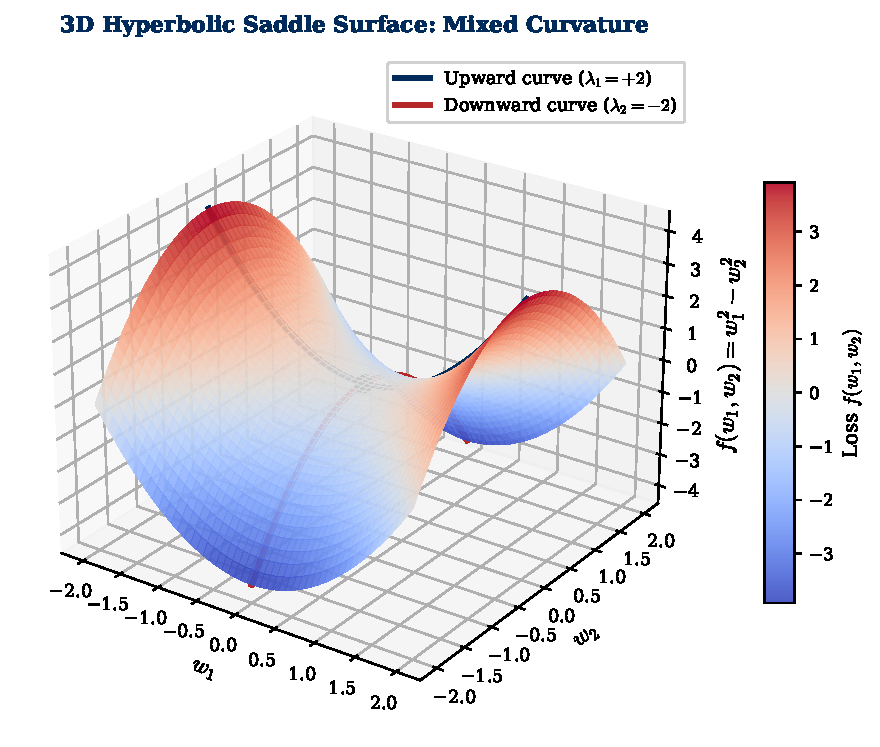
\includegraphics[width=\linewidth]{figures/saddle_point_landscape.pdf}
  \caption{High-resolution 3D visualization of the hyperbolic saddle surface, illustrating mixed eigenvalues $\lambda_1 > 0$ and $\lambda_2 < 0$.}
  \label{fig:manim_saddle_point}
\end{minipage}
\end{figure}

Figures~\ref{fig:slide_saddle_point} and~\ref{fig:manim_saddle_point} illustrate a canonical hyperbolic saddle surface $f(w_1, w_2) = w_1^2 - w_2^2$. At the origin $(0, 0)$, the gradient is zero: $\nabla f = [2w_1, -2w_2]^\top = [0, 0]^\top$. The Hessian matrix is constant:
\begin{equation}
\mathbf{H} = \begin{bmatrix} 2 & 0 \\ 0 & -2 \end{bmatrix},
\end{equation}
yielding eigenvalues $\lambda_1 = +2 > 0$ (along the $w_1$ axis) and $\lambda_2 = -2 < 0$ (along the $w_2$ axis).

\subsection{Proliferation of saddle points in high dimensions (Dauphin et al., 2014)}
\label{sec:dauphin_saddle_points}

In popular machine learning discourse, a persistent misconception is that training deep neural networks fails because first-order gradient descent gets trapped in poor local minima.

In a landmark paper presented at NeurIPS 2014, Dauphin, Bengio et al.~\cite{dauphin2014identifying} disproved this hypothesis using random matrix theory and Bray-Dean statistical physics of high-dimensional non-convex glasses. They established that:
\begin{enumerate}
  \item In a $d$-dimensional parameter space ($d \sim 10^7$ to $10^{11}$ in modern deep learning), the probability that all $d$ random eigenvalues of the Hessian share the same positive sign scales asymptotically as:
  \begin{equation}
  \mathbb{P}(\mathbf{H} \succ 0) \propto \left(\frac{1}{2}\right)^d \approx 0.
  \label{eq:saddle_point_probability}
  \end{equation}
  For $d = 1000$, $(1/2)^{1000} \approx 10^{-301}$, which is physically zero. Therefore, almost all critical points encountered in deep architectures are \textbf{saddle points}, not local minima!
  \item High-loss critical points are overwhelmingly surrounded by directions of negative curvature ($\lambda_i < 0$), providing open escape paths. True local minima exist almost exclusively near the bottom of the loss landscape, where empirical risk is already low and model generalization is strong.
  \item However, because $\|\nabla f(\mathbf{w})\| \approx 0$ in the vicinity of a saddle point, standard first-order gradient descent decelerates dramatically, spending exponential time navigating plateau-like saddle neighborhoods unless escaping noise is injected.
\end{enumerate}

\subsection{Why we are rarely interested in the global optimum}
\label{sec:global_optimum_fallacy}

In modern statistical learning, a foundational insight overturns classical intuition:
\begin{center}
\textbf{\Large\color{politoNavy} ``We are rarely interested in the global optimum!''}
\end{center}

In classical convex optimization, the global minimum is the undisputed goal. In deep learning, however, searching for the absolute global minimum of the empirical risk $\hat{\risk}_N(\mathbf{w})$ is not merely unnecessary—it is actively hazardous:
\begin{enumerate}
  \item \textbf{Overparameterization and Memorization}: Modern deep networks contain vastly more parameters than training samples ($d \gg N$). A network with millions of parameters possesses sufficient capacity to achieve zero empirical loss ($\hat{\risk}_N(\mathbf{w}^*) = 0$) by memorizing every arbitrary training sample, including mislabeled instances and random noise.
  \item \textbf{Generalization Failure}: Reaching the absolute global minimum of empirical loss often drives parameters into extreme overfitted configurations. Because the training set $\mathcal{D}_N$ is merely a finite empirical sample from underlying distribution $P$, perfectly fitting $\mathcal{D}_N$ creates huge errors on unseen test data ($\risk(h_{\mathbf{w}^*}) \gg 0$).
  \item \textbf{Sub-optimal Local Basins Generalize Better}: Any reasonable local minimum that achieves low (but non-zero) loss and resides in a broad, well-behaved basin yields vastly superior generalization compared to the degenerate empirical global optimum.
\end{enumerate}

\subsection{Flat vs. sharp minima: Hessian spectrum and test distribution generalization}
\label{sec:flat_vs_sharp_minima}

To formalize why certain local minima generalize while others overfit, optimization theory examines the \textbf{spectral flatness} of the loss basin (Hochreiter \& Schmidhuber~\cite{hochreiter1997flat}; Keskar et al.~\cite{keskar2017large}):

\begin{figure}[H]
\centering
\resizebox{0.96\linewidth}{!}{%
\begin{tikzpicture}
  % Panel A: Flat vs Sharp Minima under Distribution Shift
  \begin{axis}[
    name=plot1,
    width=8.8cm, height=6.2cm,
    axis lines=left,
    xlabel={Parameter $\mathbf{w}$},
    ylabel={Loss $\mathcal{L}(\mathbf{w})$},
    xmin=0.5, xmax=8.4,
    ymin=0, ymax=3.3,
    ticks=none,
    title={\textbf{(a) Generalization gap under distribution shift}},
    title style={font=\footnotesize, at={(0.5,1.05)}, anchor=south}
  ]
    % Train loss
    \addplot[very thick, politoNavy, domain=1.0:6.5, samples=150] 
      {1.8 + 0.05*(x-4.0)^2 - 1.5*exp(-(x-2.0)^2 / 0.10) - 1.2*exp(-(x-5.2)^2 / 1.5)}
      node[pos=1.0, right, font=\scriptsize\bfseries, text=politoNavy] {Train $\hat{\mathcal{R}}_N$};

    % Test loss (shifted by Delta w = 0.4)
    \addplot[very thick, examred, dashed, domain=1.0:6.5, samples=150] 
      {1.8 + 0.05*(x-0.4-4.0)^2 - 1.5*exp(-(x-0.4-2.0)^2 / 0.10) - 1.2*exp(-(x-0.4-5.2)^2 / 1.5)}
      node[pos=1.0, right, font=\scriptsize\bfseries, text=examred] {Test $\mathcal{R}_{\mathrm{test}}$};

    % Sharp minimum point at x = 2.0
    \draw[dotted, thick, gray!70] (axis cs:2.0, 0) -- (axis cs:2.0, 1.78);
    \fill[politoNavy] (axis cs:2.0, 0.50) circle (2.2pt);
    \fill[examred] (axis cs:2.0, 1.78) circle (2.2pt);
    \node[above left, font=\scriptsize\bfseries, text=politoNavy] at (axis cs:2.0, 0.50) {$\mathbf{w}^*_{\mathrm{sharp}}$};
    
    % Vertical gap at sharp minimum
    \draw[{Stealth[length=4pt]}-{Stealth[length=4pt]}, thick, examred] (axis cs:2.0, 0.56) -- (axis cs:2.0, 1.72);
    \node[right, font=\scriptsize\bfseries, text=examred, align=left] at (axis cs:2.05, 1.15) {Large gap\\(overfitting)};

    % Flat minimum point at x = 5.2
    \draw[dotted, thick, gray!70] (axis cs:5.2, 0) -- (axis cs:5.2, 0.75);
    \fill[politoNavy] (axis cs:5.2, 0.67) circle (2.2pt);
    \fill[examred] (axis cs:5.2, 0.75) circle (2.2pt);
    \node[below, font=\scriptsize\bfseries, text=politoNavy] at (axis cs:5.2, 0.58) {$\mathbf{w}^*_{\mathrm{flat}}$};

    % Small gap at flat minimum
    \draw[{Stealth[length=3pt]}-{Stealth[length=3pt]}, thick, intuitiongreen] (axis cs:5.2, 0.69) -- (axis cs:5.2, 0.73);
    \node[above, font=\scriptsize\bfseries, text=intuitiongreen, align=center] at (axis cs:5.3, 1.20) {Small gap\\(generalizes)};

    % Basin labels
    \node[above, font=\scriptsize\bfseries, text=politoNavy] at (axis cs:2.0, 2.7) {Sharp Minimum};
    \node[above, font=\scriptsize\bfseries, text=politoNavy] at (axis cs:5.2, 2.7) {Flat Basin};
  \end{axis}

  % Panel B: Escaping Sharp Traps via Momentum and Stochastic Noise
  \begin{axis}[
    name=plot2,
    at={($(plot1.east)+(1.8cm, 0)$)},
    anchor=west,
    width=8.8cm, height=6.2cm,
    axis lines=left,
    xlabel={Parameter $\mathbf{w}$},
    ylabel={Loss $\mathcal{L}(\mathbf{w})$},
    xmin=0.5, xmax=8.4,
    ymin=0, ymax=3.3,
    ticks=none,
    title={\textbf{(b) Escaping sharp traps via momentum \& SGD noise}},
    title style={font=\footnotesize, at={(0.5,1.05)}, anchor=south}
  ]
    % Loss landscape
    \addplot[very thick, politoNavy, domain=1.0:6.5, samples=150] 
      {1.8 + 0.05*(x-4.0)^2 - 1.5*exp(-(x-2.0)^2 / 0.10) - 1.2*exp(-(x-5.2)^2 / 1.5)}
      node[pos=1.0, right, font=\scriptsize\bfseries, text=politoNavy] {Loss $f(\mathbf{w})$};

    % Initial point w0
    \coordinate (w0) at (axis cs:1.3, 1.75);
    \shade[ball color=examred] (w0) circle (4pt) node[above left, font=\scriptsize\bfseries, text=examred] {$\mathbf{w}_0$};

    % GD path into sharp trap
    \draw[-{Stealth[length=4pt]}, thick, gray!80, dashed] (w0) to[out=-50, in=170] (axis cs:2.0, 0.52);
    \fill[gray!80] (axis cs:2.0, 0.50) circle (2.5pt);
    \node[above, font=\scriptsize\bfseries, text=gray!80, align=center] at (axis cs:1.6, 0.55) {GD stalls\\in trap};

    % Momentum trajectory flowing along the curve and overcoming barrier
    \draw[-{Stealth[length=5pt]}, very thick, deepdiveTeal] (axis cs:2.0, 0.54) 
      to[out=70, in=185] (axis cs:3.5, 1.68)
      to[out=5, in=170] (axis cs:4.4, 1.15)
      to[out=-10, in=180] (axis cs:5.2, 0.70);
    
    % Ball at the barrier
    \shade[ball color=deepdiveTeal] (axis cs:3.5, 1.70) circle (4pt);
    \node[above, font=\scriptsize\bfseries, text=deepdiveTeal, align=center] at (axis cs:3.5, 2.05) {Velocity $\mathbf{v}$ carries\\over barrier};

    % Ball in flat basin
    \shade[ball color=intuitiongreen] (axis cs:5.2, 0.67) circle (4pt);
    \node[below, font=\scriptsize\bfseries, text=intuitiongreen, align=center] at (axis cs:5.2, 0.55) {Wide Flat Basin\\(generalizes)};

    % Basin labels
    \node[above, font=\scriptsize\bfseries, text=politoNavy] at (axis cs:2.0, 2.7) {Sharp Trap};
    \node[above, font=\scriptsize\bfseries, text=politoNavy] at (axis cs:5.2, 2.7) {Flat Basin};
  \end{axis}
\end{tikzpicture}%
}
\caption{The geometry of generalization in non-convex optimization. (a) Under empirical-to-test distribution shift $\Delta \mathbf{w}$, evaluating a sharp minimum $\mathbf{w}^*_{\mathrm{sharp}}$ (large Hessian eigenvalues $\lambda_i \gg 0$) causes test loss to explode ($\Delta \mathcal{R} \gg 0$), resulting in severe overfitting. Conversely, a flat minimum $\mathbf{w}^*_{\mathrm{flat}}$ (small Hessian eigenvalues $\lambda_i \approx 0$) experiences negligible loss increase, ensuring robust generalization. (b) Standard gradient descent readily gets trapped in narrow, high-loss sharp valleys, whereas momentum velocity $\mathbf{v}$ and stochastic mini-batch noise provide the kinetic energy to escape barriers and settle into wide, flat basins.}
\label{fig:flat_vs_sharp_minima}
\end{figure}

As demonstrated in Figure~\ref{fig:flat_vs_sharp_minima}:
\begin{itemize}
  \item \textbf{Sharp Minima ($\lambda_{\max} \gg 0$)}: Characterized by narrow, steep ravines. Because the empirical training distribution $\hat{P}$ differs slightly from the true underlying distribution $P$, the test loss landscape is shifted horizontally by some small displacement $\Delta \mathbf{w}$. In a sharp well, moving $\mathbf{w}^*_{\text{sharp}} + \Delta \mathbf{w}$ catapults the loss value up the steep canyon wall, causing a catastrophic generalization gap.
  \item \textbf{Flat Minima ($\lambda_{\max} \approx 0$)}: Characterized by wide, gentle valleys. Under the exact same parameter displacement $\Delta \mathbf{w}$, the test loss remains virtually unchanged: $\mathcal{R}_{\text{test}}(\mathbf{w}^*_{\text{flat}} + \Delta \mathbf{w}) \approx \hat{\mathcal{R}}_N(\mathbf{w}^*_{\text{flat}})$. Flat minima are inherently robust to distribution shift and parameter quantization.
  \item \textbf{Kinetic Escape}: While standard batch gradient descent easily gets trapped in steep, non-generalizing local basins, momentum velocity $\mathbf{v}$ and stochastic mini-batch noise $\boldsymbol{\xi}_t$ act as dynamic perturbations that kick parameters over low barriers, naturally filtering out sharp wells in favor of expansive flat basins.
\end{itemize}

\subsection{The imperative for numerical optimization even on convex problems}
\label{sec:convex_problems_numerical_optimization}

This raises an essential theoretical question: \emph{if a machine learning problem is convex and possesses an exact analytical solution, why do we still use iterative gradient descent?}

\begin{enumerate}
  \item \textbf{Computational Complexity and Memory Scaling in OLS}:
    For linear regression, the closed-form normal equations yield $\mathbf{w}^* = (\mathbf{X}^\top \mathbf{X})^{-1}\mathbf{X}^\top \mathbf{y}$. 
    Forming the Gram matrix $\mathbf{X}^\top \mathbf{X}$ requires $\mathcal{O}(N d^2)$ operations, and inverting it via Cholesky or LU decomposition requires $\mathcal{O}(d^3)$ arithmetic operations and $\mathcal{O}(d^2)$ memory storage.
    When $d = 10^5$ (common in text, genomic, or computer vision representations), storing $d \times d$ floating-point matrices requires $40\text{ GB}$ of RAM, and computing $d^3 = 10^{15}$ operations is intractable.
    In contrast, first-order gradient descent scales as $\mathcal{O}(Nd)$ per iteration and requires only $\mathcal{O}(d)$ memory, enabling optimization on commodity hardware.
  \item \textbf{Numerical Stability and Ill-Conditioning}:
    When features are collinear, the condition number $\kappa(\mathbf{X}^\top \mathbf{X}) = (\kappa(\mathbf{X}))^2$ is squared! Direct matrix inversion suffers from catastrophic floating-point cancellation. Iterative gradient descent (especially when regularized via weight decay or early stopping) provides vastly superior numerical stability.
  \item \textbf{Non-Existence of Closed Forms in Generalized Linear Models}:
    As proven in Section~\ref{sec:no_closed_form_solution}, composing linear predictors with non-linear sigmoid or softmax links destroys linear algebra solvability. For logistic regression, closed-form inversion is mathematically impossible, leaving iterative optimization as the sole viable path.
\end{enumerate}

Although first-order gradient descent equipped with momentum and adaptive scaling provides a robust framework for navigating non-convex landscapes toward flat minima, its full-batch formulation suffers from a crushing operational bottleneck in modern data-rich environments: computing the exact gradient requires evaluating forward and backward passes across every single training observation in the dataset. When training sets scale to millions or billions of examples, evaluating a single full-batch parameter update becomes prohibitively sluggish, requiring hours or days of compute. Moreover, deterministic full-batch trajectories lack any exploratory stochasticity to jump over low energetic barriers separating sharp, overfitted wells from wide, generalizing valleys. To unlock efficient learning on massive datasets while harnessing beneficial stochastic perturbation, we must transition from deterministic batch optimization to stochastic gradient descent and mini-batch dynamics in Section~\ref{sec:sgd_and_minibatch}.

\section{Stochastic gradient descent (SGD), mini-batch dynamics, and large-scale learning bounds}
\label{sec:sgd_and_minibatch}

The empirical risk objective in supervised learning is structured as an arithmetic average of loss terms computed across individual training samples. By linearity of differentiation, computing the exact full-batch gradient requires summing the loss gradients evaluated over the entire dataset. In an era where benchmark datasets encompass millions of high-resolution images, billions of web documents, or continuous streaming logs, executing this exhaustive summation for every parameter update creates a paralyzing computational bottleneck that brings optimization to a virtual standstill.

Stochastic gradient descent (SGD) resolves this computational crisis through a profound statistical principle: an average computed over a small, randomly sampled subset of observations serves as an unbiased estimator of the true population expectation. While this subsampling injects high-frequency variance into parameter updates, this stochastic noise is far from a mere nuisance: it acts as a beneficial thermal agitation---an implicit Langevin regularizer that actively prevents parameters from settling into narrow, sharp overfitted minima, nudging the optimization trajectory toward wide, flat basins with superior generalization capabilities.

This section develops the complete theoretical and empirical foundations of stochastic and mini-batch optimization. We begin by dissecting the two computational bottlenecks of full-batch gradient descent (dataset size $n$ and parameter dimension $d$) and evaluate batch vs. stochastic vs. mini-batch estimators through concrete benchmark speedup calculations on MNIST. We then formalize the algorithmic epoch cycle, derive the statistical unbiasedness and $\mathcal{O}(1/m)$ variance reduction of mini-batch gradients, and explain why SGD does not halt at the minimum but fluctuates within a steady-state covariance cloud. Next, we establish the Robbins-Monro conditions governing almost-sure convergence, synthesize the asymptotic learning bounds of Bousquet and Bottou, and contrast all gradient estimation paradigms in an exhaustive comparative matrix. Finally, we conclude with a grand synthesis bridging linear optimization to deep representation learning.

\subsection{The two computational bottlenecks of gradient descent}
\label{sec:two_bottlenecks_gd}

Formally, the empirical risk objective $\hat{\mathcal{R}}_n(\boldsymbol{\theta})$ is defined as the arithmetic mean of loss functions evaluated over $n$ training observations:
\begin{equation}
\ell(\boldsymbol{\theta}) = \frac{1}{n} \sum_{i=1}^n \hat{\ell}_i(\boldsymbol{\theta}), \quad \text{where } \hat{\ell}_i(\boldsymbol{\theta}) \equiv \ell(f_{\boldsymbol{\theta}}(\mathbf{x}_i), y_i).
\label{eq:sum_loss_structure}
\end{equation}
By linearity of differentiation, computing the full batch gradient requires evaluating:
\begin{equation}
\nabla \ell(\boldsymbol{\theta}) = \frac{1}{n} \sum_{i=1}^n \nabla \hat{\ell}_i(\boldsymbol{\theta}).
\label{eq:full_batch_gradient}
\end{equation}

Equation~\eqref{eq:full_batch_gradient} exposes the \textbf{two fundamental bottlenecks} that render full-batch gradient descent impractical for contemporary machine learning:
\begin{enumerate}
  \item \textbf{Bottleneck 1: Number of examples $n$}. In modern datasets (ImageNet, web corpora), $n$ ranges from $10^6$ to $10^{12}$. Evaluating all $n$ forward-backward passes to execute a single parameter step takes hours or days, stalling progress completely.
  \item \textbf{Bottleneck 2: Number of parameters $d$}. Neural networks contain millions to billions of parameters ($d \sim 10^7$--$10^{11}$). Storing, communicating, and computing gradients across $d$ dimensions per sample magnifies computational overhead.
\end{enumerate}

\subsection{Batch vs. stochastic vs. mini-batch estimators and the MNIST speedup}
\label{sec:gradient_estimators_taxonomy}

To break the dataset size bottleneck $n$, we approximate the full summation over training set $\mathcal{T}$ ($|\mathcal{T}| = n$) by evaluating the gradient over a small, representative, uniformly drawn subset $\mathcal{B} \subset \mathcal{T}$ of cardinality $m \ll n$ (termed a \textbf{mini-batch}):
\begin{equation}
\frac{1}{m} \sum_{i \in \mathcal{B}} \nabla \hat{\ell}_i(\boldsymbol{\theta}) \approx \frac{1}{n} \sum_{i \in \mathcal{T}} \nabla \hat{\ell}_i(\boldsymbol{\theta}).
\label{eq:minibatch_approximation}
\end{equation}

\paragraph{A concrete benchmark speedup calculation: MNIST.}
To appreciate the computational advantage concretely, consider the canonical MNIST handwritten digit benchmark:
\begin{itemize}[noitemsep]
  \item Full training set size: $n = 60{,}000$ images.
  \item Mini-batch size: $m = 10$ images.
  \item Speedup factor per gradient update:
  \begin{equation}
  \text{Speedup} = \frac{n}{m} = \frac{60{,}000}{10} = \mathbf{6{,}000 \times \text{ faster per step!}}
  \end{equation}
\end{itemize}
In the time full-batch GD takes to evaluate a single update, mini-batch SGD executes 6,000 parameter updates, making massive progress across the loss terrain.

\subsection{Algorithmic cycle and epoch progression}
\label{sec:algorithmic_cycle_epochs}

The procedural execution of mini-batch stochastic gradient descent proceeds cyclically:
\begin{enumerate}
  \item \textbf{Initialization}: Initialize parameter vector $\boldsymbol{\theta}^{(0)} \in \R^d$ (e.g., via He or Xavier initialization).
  \item \textbf{Mini-Batch Sampling}: Uniformly sample a mini-batch $\mathcal{B} \subset \mathcal{T}$ of size $m$.
  \item \textbf{Downhill Parameter Step}: Update parameters in the negative gradient direction (optionally incorporating momentum velocity):
    \begin{equation}
    \boldsymbol{\theta} \leftarrow \boldsymbol{\theta} - \alpha \nabla \ell_{\boldsymbol{\theta}}(\mathcal{B}).
    \label{eq:minibatch_algorithmic_step}
    \end{equation}
  \item \textbf{Recurrence and Epoch Completion}: Repeat steps 2--3. When accumulated mini-batches exhaustively cover the entire training set $\mathcal{T}$, one \textbf{epoch} is completed. Training iterates across multiple epochs until validation performance plateaus.
\end{enumerate}

\begin{remark}[Constant Update Cost]
A crucial property is that the update cost per iteration is $\mathcal{O}(m \cdot d)$, which is \textbf{strictly constant regardless of the total size of dataset $\mathcal{T}$}. This invariance enables deep learning algorithms to scale gracefully to virtually infinite streaming datasets.
\end{remark}

\subsection{Statistical properties: Unbiasedness, variance scaling, and steady-state oscillations}
\label{sec:minibatch_statistics}

We formalize the statistical properties of the stochastic gradient estimator:

\paragraph{Unbiasedness.}
Let indices in mini-batch $\mathcal{B}$ be drawn uniformly at random without replacement from $\{1, \dots, n\}$. The expected value of the estimator is:
\begin{equation}
\mathbb{E}_{\mathcal{B}}\left[ \frac{1}{m} \sum_{i \in \mathcal{B}} \nabla \hat{\ell}_i(\boldsymbol{\theta}) \right] = \frac{1}{m} \sum_{i \in \mathcal{B}} \mathbb{E}\left[ \nabla \hat{\ell}_i(\boldsymbol{\theta}) \right] = \frac{1}{m} \cdot m \cdot \left( \frac{1}{n} \sum_{k=1}^n \nabla \hat{\ell}_k(\boldsymbol{\theta}) \right) = \nabla \ell(\boldsymbol{\theta}).
\label{eq:unbiased_gradient}
\end{equation}
The mini-batch gradient is an \textbf{unbiased estimator} of the true full-batch gradient.

\paragraph{Variance reduction via batch size $m$.}
Let $\sigma^2 = \frac{1}{n} \sum_{i=1}^n \|\nabla \hat{\ell}_i(\boldsymbol{\theta}) - \nabla \ell(\boldsymbol{\theta})\|_2^2$ denote sample gradient variance. The covariance of the mini-batch estimator satisfies:
\begin{equation}
\mathbb{E}\left[ \left\| \frac{1}{m} \sum_{i \in \mathcal{B}} \nabla \hat{\ell}_i(\boldsymbol{\theta}) - \nabla \ell(\boldsymbol{\theta}) \right\|_2^2 \right] = \frac{\sigma^2}{m} \left( \frac{n - m}{n - 1} \right) \approx \frac{\sigma^2}{m}.
\label{eq:minibatch_variance_reduction}
\end{equation}
Variance contracts as $\mathcal{O}(1/m)$, while computational cost scales as $\mathcal{O}(m)$. Due to the square-root law of diminishing returns ($\operatorname{StdDev} \propto 1/\sqrt{m}$), increasing batch size from $m = 32$ to $1024$ increases compute by $32\times$, but only reduces noise by $\sqrt{32} \approx 5.65\times$. Hence, moderate batch sizes ($32 \le m \le 256$) offer the optimal trade-off between parallel throughput and stochastic exploration.

\begin{figure}[H]
\centering
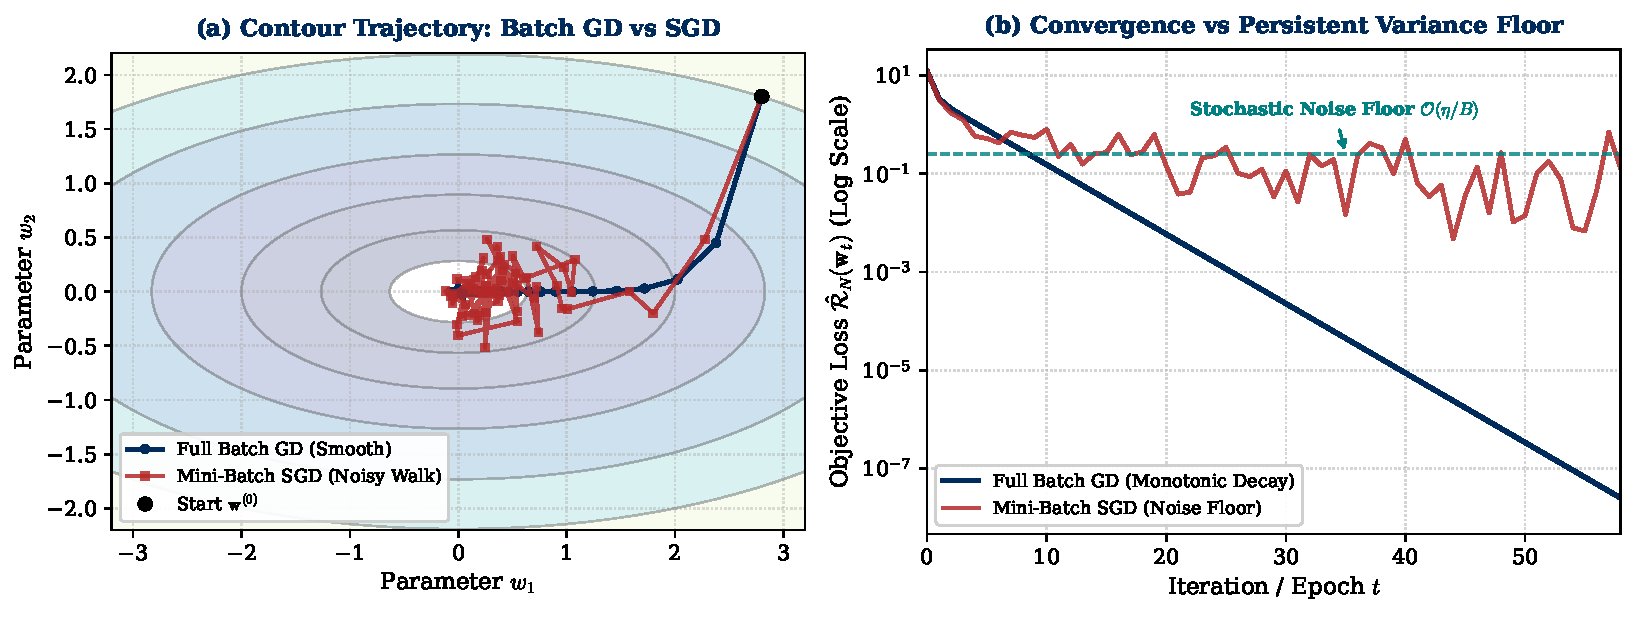
\includegraphics[width=0.95\linewidth]{figures/sgd_oscillations_dynamics.pdf}
\caption{Stochastic gradient descent dynamics: (Left) Contour trajectory showing the noisy Brownian-like walk around the loss minimum without exact stationary convergence; (Right) Parameter weight evolution over epochs on a logarithmic scale, illustrating rapid initial progress followed by persistent steady-state stochastic variance fluctuations induced by random data subsampling.}
\label{fig:slide_minibatch_dynamics}
\end{figure}

\paragraph{Steady-state fluctuations around the minimum.}
As illustrated in Figure~\ref{fig:slide_minibatch_dynamics}, a defining hallmark of SGD is that \textbf{it does not halt at the minimum}:
\begin{equation}
\lim_{t \to \infty} \mathbb{E}\left[ \|\boldsymbol{\theta}_t - \boldsymbol{\theta}^*\|_2^2 \right] \approx \mathcal{O}(\alpha \sigma^2).
\end{equation}
Even when the true gradient vanishes at the minimizer ($\nabla \ell(\boldsymbol{\theta}^*) = \mathbf{0}$), individual sample gradients $\nabla \hat{\ell}_i(\boldsymbol{\theta}^*)$ do not vanish! Consequently, mini-batch gradients retain stochastic noise, causing parameters to wander indefinitely in a steady-state covariance cloud around $\boldsymbol{\theta}^*$.

\subsection{Robbins-Monro convergence conditions for stochastic optimization}
\label{sec:robbins_monro}

To extinguish persistent stochastic oscillations and guarantee almost sure convergence to a stationary point ($\lim_{t \to \infty} \boldsymbol{\theta}_t = \boldsymbol{\theta}^*$), the learning rate sequence $\{\alpha_t\}_{t=1}^\infty$ must be decayed.

In their foundational 1951 paper on stochastic approximation, Herbert Robbins and Sutton Monro~\cite{robbins1951stochastic} established the necessary and sufficient conditions:
\begin{equation}
\sum_{t=1}^\infty \alpha_t = \infty \quad \text{and} \quad \sum_{t=1}^\infty \alpha_t^2 < \infty.
\label{eq:robbins_monro_conditions}
\end{equation}
\begin{itemize}[noitemsep]
  \item \textbf{Condition 1 ($\sum \alpha_t = \infty$)}: Guarantees infinite exploration horizon. The cumulative distance parameters can travel is unbounded, ensuring the optimizer never stalls before reaching the minimum basin.
  \item \textbf{Condition 2 ($\sum \alpha_t^2 < \infty$)}: Guarantees variance extinction. Because cumulative error variance accumulates as $\sum \alpha_t^2 \sigma^2 < \infty$, stochastic fluctuations vanish asymptotically at $\boldsymbol{\theta}^*$.
\end{itemize}

\subsection{Asymptotic upper bounds for large-scale learning (Bottou \& Bousquet, 2008)}
\label{sec:bottou_bousquet_bounds}

The seminal theoretical framework of Léon Bottou and Olivier Bousquet~\cite{bottou2008tradeoffs} (NeurIPS 2008, \emph{``The Tradeoffs of Large Scale Learning''}) rigorously demonstrates why SGD achieves superior generalization compared to full-batch GD under bounded computational budgets.

Consider a convex learning problem with training set size $n$, parameter dimension $d$, and objective condition number $\kappa$. We seek to achieve target accuracy $\rho > 0$ on excess true risk:
\begin{equation}
\left| \ell(h_{\boldsymbol{\theta}}) - \ell(f^*) \right| < \rho,
\label{eq:excess_risk_target}
\end{equation}
where $\ell(h_{\boldsymbol{\theta}})$ is the expected risk of the learned hypothesis, and $\ell(f^*)$ is the Bayes optimal risk.

\begin{table}[H]
\centering
\caption{Asymptotic upper bounds for reaching excess risk $\rho$ on convex problems (Bottou \& Bousquet, NeurIPS 2008). Here $\kappa$ and $\nu$ are constants governing objective conditioning and gradient variance.}
\label{tab:bottou_bousquet_bounds}
\begin{tabularx}{0.92\textwidth}{lXX}
\toprule
\textbf{Optimization Algorithm} & \textbf{Computational Cost per Iteration} & \textbf{Iterations to Reach Target Error $\rho$} \\
\midrule
Full Batch Gradient Descent (GD) & $\mathcal{O}(n \cdot d)$ & $\mathcal{O}\left(\kappa \log \frac{1}{\rho}\right)$ \\
\addlinespace
Stochastic Gradient Descent (SGD) & $\mathcal{O}(d)$ & $\frac{\nu \kappa^2}{\rho} + o\left(\frac{1}{\rho}\right)$ \\
\bottomrule
\end{tabularx}
\end{table}

\paragraph{The profound theoretical implication: Total computational cost.}
Evaluating the total computational work required to reach accuracy $\rho$:
\begin{align}
\text{Total Work}_{\text{GD}} &= \mathcal{O}(nd) \times \mathcal{O}\left(\kappa \log \frac{1}{\rho}\right) = \mathcal{O}\left( n \cdot d \cdot \kappa \log \frac{1}{\rho} \right), \label{eq:total_work_gd} \\
\text{Total Work}_{\text{SGD}} &= \mathcal{O}(d) \times \left( \frac{\nu \kappa^2}{\rho} + o\left(\frac{1}{\rho}\right) \right) = \mathcal{O}\left( \frac{d \cdot \nu \kappa^2}{\rho} \right). \label{eq:total_work_sgd}
\end{align}

\begin{examinsight}[Oral Exam Milestone: Why SGD Generalizes Better]
Observe the fundamental distinction between Equations~\eqref{eq:total_work_gd} and~\eqref{eq:total_work_sgd}:
\begin{center}
\textbf{The total computational cost of SGD does NOT depend on the number of training examples $n$!}
\end{center}
In large-scale machine learning where computation time is limited:
\begin{itemize}[noitemsep]
  \item \textbf{Full Batch GD} spends vast computational resources computing ultra-precise gradients over a fixed, finite dataset $\mathcal{D}_n$, driving empirical training error to zero but over-fitting sample noise.
  \item \textbf{SGD} takes cheap, noisy steps that each touch new, unvisited samples. For a fixed computational budget of floating-point operations (FLOPs), SGD processes orders of magnitude more distinct data samples from distribution $P$.
\end{itemize}
Because statistical generalization error is bounded by the total amount of unique data processed rather than optimization precision on a small set, \textbf{SGD achieves strictly superior generalization error (true risk)}!
\end{examinsight}

\subsection{Practical considerations in modern deep learning SGD}
\label{sec:practical_sgd_deep_learning}

To conclude the optimization framework, we synthesize five foundational practical principles for deploying SGD in contemporary neural networks:

\begin{enumerate}
  \item \textbf{Data Shuffling to Eliminate Ordering Bias}:
    Mini-batches must be drawn by randomly shuffling the dataset at the start of every epoch. If data exhibits sequential correlation (e.g., all class~1 digits grouped together), sequential mini-batches will violently drag parameters toward class~1, causing catastrophic forgetting of preceding classes and inducing cyclic optimization orbits.
  \item \textbf{Hardware Parallelization and SIMD Efficiency}:
    While pure SGD ($m = 1$) is optimal in theory, single-sample operations fail to exploit GPU parallelism. Mini-batch sizes $m \in \{32, 64, 128, 256, 512\}$ are chosen to match GPU Streaming Multiprocessor warp sizes and saturate Tensor Core matrix multiplication units (GEMM).
  \item \textbf{Two-Phase Optimization Dynamics}:
    SGD exhibits an asymmetric temporal profile: \textbf{remarkably rapid initial progress} in early epochs as parameters drop down steep macro-gradients into low-loss valleys, followed by \textbf{slow asymptotic fine-tuning} where parameter wanderings are dominated by gradient variance.
  \item \textbf{Implicit Regularization of Small Mini-Batches}:
    Small mini-batches inject high stochastic gradient noise ($\propto \sigma^2 / m$). This noise acts as an implicit regularizer, preventing parameters from settling into sharp overfitted minima and nudging trajectories into wide flat basins. However, because variance is high, practitioners must reduce the learning rate $\alpha$ (or apply linear learning rate scaling $\alpha \propto m$) to preserve numerical stability.
  \item \textbf{The Practitioner's Fundamental Maxim}:
    This crystallizes the ultimate operational rule of deep learning optimization:
    \begin{center}
    \textbf{\large\color{politoNavy} ``SGD can find a low value of the loss quickly enough to be useful, even if it's not a minimum.''}
    \end{center}
    In real-world engineering, achieving an exact stationary point ($\nabla \ell = \mathbf{0}$) is neither required nor desirable. Finding a robust, flat basin with low empirical loss within practical time constraints delivers state-of-the-art generalization.
\end{enumerate}

\clearpage
\enlargethispage{\baselineskip}
\subsection{Systematic comparison of gradient descent paradigms}
\label{sec:systematic_comparison}

Table~\ref{tab:gradient_comparison} synthesizes the mathematical, computational, and algorithmic trade-offs across the gradient descent family.

\begin{table}[H]
\centering
\small
\renewcommand{\arraystretch}{0.90}
\caption{Systematic comparison of Batch Gradient Descent, Stochastic Gradient Descent (SGD), and Mini-Batch SGD.}
\label{tab:gradient_comparison}
\begin{tabularx}{\textwidth}{lXXX}
\toprule
\textbf{Property} & \textbf{Batch Gradient Descent} & \textbf{Stochastic GD (SGD)} & \textbf{Mini-Batch SGD} \\

\midrule
\textbf{Batch Size $B$} & $B = n$ (full dataset) & $B = 1$ (single sample) & $1 < B < n$ (typically $32$--$512$) \\
\textbf{Cost per Step} & $\mathcal{O}(n \cdot d)$ & $\mathcal{O}(d)$ & $\mathcal{O}(B \cdot d)$ \\
\textbf{Gradient Variance} & Zero (deterministic) & High ($\sigma^2$) & Controlled ($\sigma^2 / B$) \\
\textbf{Convergence Path} & Monotonic \& smooth & Erratic \& oscillatory & Controlled variance cloud \\
\textbf{Hardware Affinity} & Memory bound on large $n$ & Poor GPU SIMD usage & Highly optimized for GPU BLAS \\
\textbf{Saddle Point Escape} & Vulnerable to stall & High escape ability & Strong escape via noise \\
\textbf{Scaling with $n$} & Total work scales with $n$ & Total work independent of $n$ & Total work independent of $n$ \\
\textbf{Generalization} & Prone to sharp traps & Excellent (flat basins) & Optimal (balanced noise) \\
\bottomrule
\end{tabularx}
\end{table}

\subsection{Chapter synthesis and roadmap to representation learning}
\label{sec:chapter3_synthesis}

Across Chapters~1 through~3, we have traversed the foundational triad of statistical machine learning:
\begin{enumerate}[noitemsep,topsep=2pt,parsep=0pt,partopsep=0pt]
  \item \textbf{Statistical foundations (Chapter~1)}: Defining learning paradigms, hypothesis spaces, and the fundamental trade-off between empirical risk and true risk.
  \item \textbf{Decision-theoretic limits (Chapter~2)}: Formulating the Bayes optimal predictor, irreducible noise, and the estimation/approximation trade-off governing model capacity.
  \item \textbf{Loss geometry and optimization (Chapter~3)}: Moving from the non-convex pathologies of squared error in classification to cross-entropy, and replacing intractable analytical matrix inversions with first-order iterative methods (GD, Momentum, and Mini-batch SGD).
\end{enumerate}

The decisive realization uniting this theoretical arc is that \textbf{optimization in machine learning is subservient to generalization}. Unlike classical numerical analysis, where reaching an exact critical point ($\nabla \ell = \mathbf{0}$) is paramount, deep learning exploits stochastic gradient noise, momentum dynamics, and early stopping as implicit regularizers that bias trajectories away from sharp overfitted traps and toward wide, flat basins with superior test performance.

However, all models examined thus far have relied on \textbf{fixed linear representations} $\mathbf{w}^\top \mathbf{x} + b$. Even when paired with cross-entropy and trained via mini-batch SGD, a linear hyperplane cannot separate nonlinearly distributed data (such as the classical XOR problem or complex perceptual manifolds). To transcend this expressivity bottleneck, machine learning diverges into two great paradigms:
\begin{itemize}[noitemsep,topsep=2pt,parsep=0pt,partopsep=0pt]
  \item \textbf{Implicit feature spaces (Kernel Methods and SVMs)}: Projecting inputs into high- (or infinite-) dimensional Hilbert spaces via the kernel trick while retaining convex dual optimization.
  \item \textbf{Explicit hierarchical representations (Deep Neural Networks)}: Learning parameterized feature transformations end-to-end via composite nonlinear layers, where optimization gradients are propagated through intermediate representations using the chain rule (Backpropagation).
\end{itemize}
These representation learning paradigms form the core of the upcoming chapters.



\chapter{Deep feedforward networks and backpropagation}
\label{sec:deep_feedforward_and_backpropagation}

The quest to construct artificial intelligence originated with a profound biological ambition: to emulate the computational architecture of the human brain. While classical machine learning algorithms—such as Ordinary Least Squares, Ridge regression, and linear support vector machines—operate by mapping inputs directly to predictions via fixed, handcrafted feature representations, natural sensory perception defies static linear modeling. Human cognition effortlessly navigates complex perceptual manifolds: recognizing a handwritten digit, segmenting a tumor in an acoustic scan, or parsing visual scenes across dramatic shifts in illumination, scale, and orientation.

To transcend the rigid confines of linear predictors, connectionist theory introduced the \textbf{artificial neural network}—a massively parallel computational architecture composed of elementary interconnected processing nodes. This intellectual journey began with Frank Rosenblatt's 1958 Perceptron, an elegant bio-inspired unit that computed affine combinations thresholded by a step function. Yet, as Marvin Minsky and Seymour Papert demonstrated in their devastating 1969 critique, single-layer perceptrons possess a fatal geometric blind spot: bounded strictly by linear separability, they fail on elementary non-linear predicates as simple as the Exclusive-OR (XOR) function, precipitating the First AI Winter.

The modern deep learning revolution was born from overcoming this linear barrier through two foundational mathematical innovations. First, by cascading multiple layers of neurons equipped with continuous, non-linear activation functions into \textbf{Multilayer Perceptrons (MLPs)}, networks acquire the capacity for \textbf{representation learning}. Rather than relying on human engineers to handcraft feature spaces, deep architectures automatically fold, stretch, and warp input coordinate space, transforming complex non-linear manifolds into representations that are cleanly linearly separable. The celebrated Hornik-Cybenko Universal Approximation Theorem formalizes this expressive power, guaranteeing that feedforward networks can approximate any continuous function on a compact domain to arbitrary precision.

Yet, representational power is useless without an efficient training engine. Because deep compositions of non-linear activations entangle parameters in transcendental algebraic systems, closed-form matrix inversions are mathematically impossible, and numerical finite differences require an intractable $\mathcal{O}(W^2)$ computational complexity. This computational gridlock was broken by formulating deep networks as Directed Acyclic Graphs (DAGs) and applying reverse-mode automatic differentiation: the \textbf{Backpropagation algorithm}. By propagating adjoint error sensitivities backward through the network in a single sweep, backpropagation evaluates the exact gradient across millions of parameters in linear $\mathcal{O}(W)$ time, establishing the foundational mathematical engine of contemporary artificial intelligence.

\section{The perceptron}
\label{sec:perceptron_and_linear_separability}

The quest to construct artificial intelligence originated with a profound biological ambition: to understand and replicate the computational mechanisms of the brain. In the 1940s and 1950s, the emergence of early digital computing was defined by von Neumann architectures designed for serial instruction execution and exact symbolic arithmetic. While these mechanical and electronic calculators could perform millions of numerical operations per second, they proved utterly incapable of solving elementary perceptual tasks that animal brains resolve effortlessly and instantaneously---such as recognizing a visual pattern, distinguishing spoken phonemes, or adapting to sensory variations in an uncertain environment.

This striking divergence highlighted a fundamental insight: biological intelligence does not operate via centralized instruction registers, brittle algorithmic decision trees, or hand-crafted symbolic lookup tables. Instead, cognitive function emerges from the collective dynamics of billions of interconnected, elementary biological cells---neurons---transmitting electrical impulses across plastic synaptic junctions. Despite individual biological neurons operating at millisecond timescales (orders of magnitude slower than electronic switching circuits), their massive parallel connectivity enables robust associative memory, real-time sensory processing, and the ability to learn directly from experience.

Inspired by these neurophysiological observations, early cyberneticians and cognitive scientists---beginning with Warren McCulloch and Walter Pitts in 1943, Donald Hebb in 1949, and culminating in Frank Rosenblatt in 1958---sought to abstract the physical machinery of the biological neuron into an elementary mathematical learning unit. By modeling synaptic plasticity as adjustable numerical weights and dendritic summation as an affine score thresholded by an excitation activation, they aimed to create an artificial computing system capable of discovering patterns and categorizing sensory observations autonomously without explicit human programming.

\subsection{Architecture and convergence}
\label{sec:biological_and_artificial_neuron}
\label{sec:perceptron_learning_algorithm}

\paragraph{Biological morphology and Rosenblatt's artificial threshold unit.}
In biological nervous systems, an individual neuron consists of four primary morphological structures:
\begin{itemize}[noitemsep,topsep=2pt,parsep=0pt,partopsep=0pt]
  \item \textbf{Dendrites}: Branching nerve fibers that receive incoming chemical neurotransmitter signals from adjacent upstream neurons across synaptic clefts.
  \item \textbf{Soma (Cell Body)}: The metabolic hub containing the nucleus, which integrates and accumulates incoming post-synaptic electrical potentials over space and time.
  \item \textbf{Axon}: A long, slender nerve transmission cable (often insulated by fatty myelin sheaths) that propagates an all-or-nothing action potential (voltage spike) down its length once the soma's membrane potential surpasses an excitation threshold.
  \item \textbf{Synapses}: Chemical junctions connecting axon terminal boutons to recipient dendrites, where biological synaptic plasticity modulates the efficacy of electrical transmission.
\end{itemize}

In 1958, Frank Rosenblatt~\cite{rosenblatt1958perceptron} formalized this biological mechanism into the \textbf{Perceptron}. Given an input vector of sensory features $\mathbf{x} = [x_1, \dots, x_d]^\top \in \R^d$, the artificial neuron associates each input channel with a tunable real-valued weight $w_j \in \R$, incorporates a scalar bias threshold $b \in \R$, and computes a linear pre-activation score:
\begin{equation}
z \triangleq \mathbf{w}^\top \mathbf{x} + b = \sum_{j=1}^d w_j x_j + b.
\label{eq:perceptron_preactivation}
\end{equation}
The continuous scalar score $z$ is then passed through a discontinuous Heaviside step activation function to produce a binary classification decision:
\begin{equation}
\hat{y} = f(z) = \operatorname{sgn}(z) = \begin{cases} +1 & \text{if } \mathbf{w}^\top \mathbf{x} + b \ge 0, \\ -1 & \text{if } \mathbf{w}^\top \mathbf{x} + b < 0. \end{cases}
\label{eq:perceptron_activation}
\end{equation}

\begin{figure}[H]
\centering
\begin{tikzpicture}[scale=0.92, every node/.style={transform shape}]
  % Left Panel: Biological Neuron
  \begin{scope}[shift={(0,0)}]
    \node[font=\bfseries\sffamily\color{politoNavy}] at (3.0, 2.7) {(a) Biological Neuron Anatomy};
    
    % Dendrites branching
    \draw[thick, deepblue] (0.2, 1.8) -- (1.5, 1.2);
    \draw[thick, deepblue] (0.0, 1.0) -- (1.5, 0.8);
    \draw[thick, deepblue] (0.3, 0.0) -- (1.5, 0.4);
    \draw[thick, deepblue] (-0.2, 1.5) -- (0.8, 1.2);
    \draw[thick, deepblue] (-0.2, 0.4) -- (0.8, 0.6);
    \node[font=\scriptsize\color{deepblue}, align=center] at (0.3, -0.4) {Dendrites\\(Inputs $\mathbf{x}$)};

    % Soma (cell body)
    \draw[fill=deepblue!15, draw=deepblue, very thick] (2.2, 0.8) circle (0.85);
    \draw[fill=deepblue!40, draw=deepblue] (2.2, 0.8) circle (0.35);
    \node[font=\scriptsize\bfseries\color{politoNavy}, align=center] at (2.2, 0.8) {Soma\\($\sum$)};
    \node[font=\scriptsize\color{deepblue}, align=center] at (2.2, -0.4) {Cell Body\\(Accumulator)};

    % Axon with myelin sheath
    \draw[ultra thick, deepblue] (3.05, 0.8) -- (5.2, 0.8);
    \foreach \x in {3.3, 3.9, 4.5} {
      \draw[fill=skyBlue!40, draw=politoNavy, rounded corners=2pt] (\x, 0.60) rectangle (\x+0.45, 1.00);
    }
    \node[font=\scriptsize\color{deepblue}, align=center] at (4.1, -0.4) {Axon Cable\\(Transmission)};

    % Axon Terminals / Synapses
    \draw[thick, deepblue] (5.2, 0.8) -- (5.9, 1.3);
    \draw[thick, deepblue] (5.2, 0.8) -- (6.0, 0.8);
    \draw[thick, deepblue] (5.2, 0.8) -- (5.9, 0.3);
    \foreach \pos in {(5.9, 1.3), (6.0, 0.8), (5.9, 0.3)} {
      \fill[examred] \pos circle (2.2pt);
    }
    \node[font=\scriptsize\color{examred}, align=center] at (6.0, -0.4) {Synaptic Boutons\\(Output $\hat{y}$)};
  \end{scope}

  % Vertical Separator
  \draw[dashed, gray!40, thick] (6.9, -0.8) -- (6.9, 3.1);

  % Right Panel: Artificial Perceptron
  \begin{scope}[shift={(7.8,0)}]
    \node[font=\bfseries\sffamily\color{politoNavy}] at (3.5, 2.7) {(b) Rosenblatt's Artificial Perceptron};

    % Inputs
    \node[circle, draw=deepblue, fill=deepblue!10, thick, inner sep=2pt, font=\footnotesize] (x1) at (0, 1.8) {$x_1$};
    \node[circle, draw=deepblue, fill=deepblue!10, thick, inner sep=2pt, font=\footnotesize] (x2) at (0, 0.9) {$x_2$};
    \node[font=\footnotesize] (xdots) at (0, 0.2) {$\vdots$};
    \node[circle, draw=deepblue, fill=deepblue!10, thick, inner sep=2pt, font=\footnotesize] (xd) at (0, -0.6) {$x_d$};
    \node[circle, draw=gray!70, fill=gray!10, thick, inner sep=2pt, font=\footnotesize] (xb) at (0, -1.4) {$+1$};

    % Summation Node
    \node[circle, draw=politoNavy, fill=politoNavy!15, very thick, inner sep=5pt, font=\normalsize] (sum) at (2.8, 0.6) {$\sum$};
    \node[font=\tiny\color{politoNavy}, below=2pt of sum] {$z = \mathbf{w}^\top\mathbf{x} + b$};

    % Connections with weights
    \draw[-{Stealth}, thick] (x1) -- node[above, font=\scriptsize] {$w_1$} (sum);
    \draw[-{Stealth}, thick] (x2) -- node[above, font=\scriptsize] {$w_2$} (sum);
    \draw[-{Stealth}, thick] (xd) -- node[below, font=\scriptsize] {$w_d$} (sum);
    \draw[-{Stealth}, thick, dashed] (xb) -- node[below, font=\scriptsize] {$b$} (sum);

    % Activation Function Block
    \node[rectangle, draw=intuitiongreen, fill=intuitiongreen!15, thick, inner sep=5pt, font=\footnotesize, right=0.9cm of sum] (act) {$\operatorname{sgn}(z)$};

    \draw[-{Stealth}, thick] (sum) -- node[above, font=\scriptsize] {$z$} (act);

    % Output
    \node[right=0.9cm of act, font=\footnotesize\bfseries] (out) {$\hat{y} \in \{-1, +1\}$};
    \draw[-{Stealth}, very thick, examred] (act) -- (out);
  \end{scope}
\end{tikzpicture}
\caption{Morphological and mathematical correspondence between biological and artificial neural processing. (a) A biological neuron integrates post-synaptic potentials across dendrites into the metabolic soma, firing an action potential down the myelinated axon toward synaptic terminals. (b) Rosenblatt's artificial perceptron models this mechanism: numerical inputs $x_j$ are modulated by synaptic parameters $w_j$, accumulated by affine summation $z = \mathbf{w}^\top \mathbf{x} + b$, and thresholded by a Heaviside sign function to produce binary classification $\hat{y} \in \{-1, +1\}$.}
\label{fig:biological_vs_artificial_neuron}
\end{figure}

\paragraph{Decision hyperplane geometry.}
Geometrically, the equation $\mathbf{w}^\top \mathbf{x} + b = 0$ defines a $(d-1)$-dimensional \textbf{decision hyperplane} that partitions the $d$-dimensional input space $\mathcal{X} \subseteq \R^d$ into two open half-spaces: a positive half-space where $\mathbf{w}^\top \mathbf{x} + b \ge 0$ (yielding $\hat{y} = +1$) and a negative half-space where $\mathbf{w}^\top \mathbf{x} + b < 0$ (yielding $\hat{y} = -1$). The parameter vector $\mathbf{w} \in \R^d$ is the orthogonal normal vector to the hyperplane pointing directly toward the positive decision half-space. The scalar bias $b \in \R$ offsets the hyperplane from the origin, establishing a signed perpendicular Euclidean distance of $\frac{|b|}{\|\mathbf{w}\|_2}$.

\begin{figure}[H]
\centering
\begin{tikzpicture}[scale=1.15]
  % Axes
  \draw[-{Stealth}, gray!70, thick] (-1.0, 0) -- (5.0, 0) node[right, font=\footnotesize] {$x_1$};
  \draw[-{Stealth}, gray!70, thick] (0, -1.0) -- (0, 4.2) node[above, font=\footnotesize] {$x_2$};

  % Half-space shading
  \fill[deepblue!8, opacity=0.8] (-0.8, 3.8) -- (4.2, 0.46) -- (4.5, 3.8) -- (-0.8, 3.8) -- cycle;
  \fill[examred!8, opacity=0.8] (-0.8, 3.8) -- (4.2, 0.46) -- (4.2, -0.8) -- (-0.8, -0.8) -- cycle;

  % Hyperplane: w1*x1 + w2*x2 + b = 0
  \draw[very thick, politoNavy] (-0.6, 2.5) -- (4.4, -0.8) node[right, font=\footnotesize, align=left] {Decision Hyperplane:\\$\mathbf{w}^\top \mathbf{x} + b = 0$};

  % Normal vector w from a point on the line (1.5, 1.0)
  \coordinate (P) at (1.5, 1.0);
  \draw[-{Stealth[length=6pt]}, ultra thick, intuitiongreen] (P) -- ++(1.0, 1.5) node[above right, font=\footnotesize\bfseries] {$\mathbf{w}$ (Orthogonal Normal Vector)};

  % Perpendicular projection from Origin (0,0) to line
  \coordinate (Proj) at (0.923, 1.385);
  \draw[dashed, thick, gray!80] (0, 0) -- (Proj);
  \draw[thick, gray!80] (0.8, 1.2) -- (0.95, 1.1) -- (1.07, 1.28);
  \node[left, font=\scriptsize\bfseries, text=politoNavy] at (0.45, 0.75) {$d = \frac{|b|}{\|\mathbf{w}\|_2}$};

  % Data points: Positive Class (+1)
  \node[star, star points=5, star point ratio=2.2, draw=deepblue, fill=deepblue!30, thick, inner sep=2.5pt] at (2.2, 2.6) {};
  \node[star, star points=5, star point ratio=2.2, draw=deepblue, fill=deepblue!30, thick, inner sep=2.5pt] at (3.5, 2.1) {};
  \node[star, star points=5, star point ratio=2.2, draw=deepblue, fill=deepblue!30, thick, inner sep=2.5pt] at (1.2, 3.1) {};
  \node[star, star points=5, star point ratio=2.2, draw=deepblue, fill=deepblue!30, thick, inner sep=2.5pt] at (3.8, 3.3) {};
  \node[font=\footnotesize\bfseries, text=deepblue] at (3.2, 3.8) {Positive Half-Space: $\mathbf{w}^\top\mathbf{x} + b > 0$};

  % Data points: Negative Class (-1)
  \node[circle, draw=examred, fill=examred!20, thick, inner sep=2.5pt] at (0.5, 0.5) {};
  \node[circle, draw=examred, fill=examred!20, thick, inner sep=2.5pt] at (1.5, -0.2) {};
  \node[circle, draw=examred, fill=examred!20, thick, inner sep=2.5pt] at (2.8, -0.4) {};
  \node[circle, draw=examred, fill=examred!20, thick, inner sep=2.5pt] at (0.2, 1.2) {};
  \node[font=\footnotesize\bfseries, text=examred] at (1.5, -0.7) {Negative Half-Space: $\mathbf{w}^\top\mathbf{x} + b < 0$};

  % Origin
  \fill (0,0) circle (2pt) node[below left, font=\footnotesize] {$\mathbf{0}$};
\end{tikzpicture}
\caption{The geometry of the linear decision boundary defined by the perceptron. The parameter vector $\mathbf{w} \in \mathbb{R}^d$ is the orthogonal normal vector to the hyperplane pointing directly toward the positive decision half-space. The scalar bias $b \in \mathbb{R}$ offsets the hyperplane from the origin, establishing a signed perpendicular Euclidean distance of $\frac{|b|}{\|\mathbf{w}\|_2}$.}
\label{fig:hyperplane_geometry}
\end{figure}

\paragraph{The perceptron learning algorithm.}
Given a supervised training dataset $\mathcal{D} = \{(\mathbf{x}_i, y_i)\}_{i=1}^n$ with binary labels $y_i \in \{-1, +1\}$, the perceptron learning algorithm operates in an online, mistake-driven fashion. Parameters are initialized arbitrarily (typically $\mathbf{w}^{(0)} = \mathbf{0}, b^{(0)} = 0$).

At step $t$, the algorithm inspects an incoming training instance $(\mathbf{x}_i, y_i)$. If the current hypothesis correctly classifies the instance ($y_i (\mathbf{w}^{(t)\top} \mathbf{x}_i + b^{(t)}) > 0$), no modification is made. If the instance is misclassified ($y_i (\mathbf{w}^{(t)\top} \mathbf{x}_i + b^{(t)}) \le 0$), parameters are updated via the additive correction:
\begin{align}
\mathbf{w}^{(t+1)} &= \mathbf{w}^{(t)} + \eta y_i \mathbf{x}_i, \label{eq:perceptron_update_w} \\
b^{(t+1)} &= b^{(t)} + \eta y_i R^2, \label{eq:perceptron_update_b}
\end{align}
where $\eta > 0$ is the learning rate (often set to $\eta = 1$ without loss of generality, as scaling both sides leaves the sign of predictions unchanged), and $R = \max_i \|\mathbf{x}_i\|_2$ is the radius of the smallest sphere enclosing the data. In parameter space, this update executes vector addition; in input space, it rotates the decision hyperplane directly toward the misclassified sample, pulling it into the correct decision region.

\begin{figure}[H]
\centering
\begin{minipage}{0.48\linewidth}
  \centering
  \begin{tikzpicture}[scale=1.05]
    \node[font=\footnotesize\bfseries\color{politoNavy}] at (1.5, 3.2) {(a) Parameter Space: Vector Correction};
    \draw[-{Stealth}, gray!50] (-0.5, 0) -- (3.2, 0) node[right, font=\tiny] {$w_1$};
    \draw[-{Stealth}, gray!50] (0, -0.5) -- (0, 3.0) node[above, font=\tiny] {$w_2$};
    
    % w(t)
    \coordinate (W0) at (0.8, 1.8);
    \draw[-{Stealth[length=6pt]}, very thick, politoNavy] (0, 0) -- (W0) node[above left, font=\footnotesize] {$\mathbf{w}^{(t)}$};
    
    % Misclassified sample vector y_i * x_i (positive class: +x_i)
    \coordinate (X) at (1.6, -0.4);
    \draw[-{Stealth[length=6pt]}, very thick, examred] (W0) -- ++(X) node[midway, above right, font=\footnotesize] {$+y_i \mathbf{x}_i$};
    
    % w(t+1)
    \coordinate (W1) at ($(W0) + (X)$);
    \draw[-{Stealth[length=6pt]}, very thick, intuitiongreen] (0, 0) -- (W1) node[right, font=\footnotesize\bfseries] {$\mathbf{w}^{(t+1)}$};
    
    \node[draw=politoNavy, fill=politoNavy!5, rounded corners, font=\scriptsize, align=center] at (1.5, -0.8) {$\mathbf{w}^{(t+1)} = \mathbf{w}^{(t)} + \eta y_i \mathbf{x}_i$};
  \end{tikzpicture}
\end{minipage}\hfill
\begin{minipage}{0.48\linewidth}
  \centering
  \begin{tikzpicture}[scale=1.05]
    \node[font=\footnotesize\bfseries\color{politoNavy}] at (1.5, 3.2) {(b) Input Space: Boundary Rotation};
    \draw[-{Stealth}, gray!50] (-1.0, 0) -- (3.2, 0) node[right, font=\tiny] {$x_1$};
    \draw[-{Stealth}, gray!50] (0, -1.0) -- (0, 3.0) node[above, font=\tiny] {$x_2$};

    % Old boundary w(t)^T x = 0
    \draw[thick, politoNavy, dashed] (-0.9, 0.4) -- (2.5, -1.1) node[below right, font=\tiny, align=left] {Old boundary:\\$\mathbf{w}^{(t)\top}\mathbf{x}=0$};
    
    % Misclassified point x_i (positive class y_i = +1)
    \node[star, star points=5, star point ratio=2.2, draw=examred, fill=examred!30, thick, inner sep=2.5pt, label={right:\scriptsize $\mathbf{x}_i \ (y_i = +1)$}] (xi) at (1.2, -0.8) {};

    % New boundary w(t+1)^T x = 0
    \draw[very thick, intuitiongreen] (-0.8, -0.6) -- (2.0, 2.2) node[above right, font=\tiny, align=left] {New boundary:\\$\mathbf{w}^{(t+1)\top}\mathbf{x}=0$};

    % Rotation arrow
    \draw[-{Stealth}, thick, deepdiveTeal] (1.8, -0.7) to[bend right=25] (1.3, 1.4) node[midway, right, font=\tiny] {Boundary rotates toward $\mathbf{x}_i$};
  \end{tikzpicture}
\end{minipage}
\caption{Geometric dynamics of the Perceptron Learning Algorithm update. (a) In parameter space, whenever a training sample $(\mathbf{x}_i, y_i)$ is misclassified, the algorithm performs vector addition $\mathbf{w}^{(t+1)} = \mathbf{w}^{(t)} + y_i \mathbf{x}_i$. (b) In input space, adding $y_i \mathbf{x}_i$ rotates the orthogonal decision hyperplane directly toward the misclassified sample, pulling it into the correct decision region.}
\label{fig:perceptron_learning_dynamics}
\end{figure}

\paragraph{Novikoff's convergence theorem.}
The historical significance of Rosenblatt's perceptron stems from the fact that it was the first machine learning model accompanied by a rigorous mathematical convergence proof, formalized by Albert Novikoff in 1962~\cite{novikoff1962convergence}.

\begin{theorem}[Novikoff's Perceptron Convergence Theorem]
\label{thm:novikoff_convergence}
Let $\mathcal{D} = \{(\mathbf{x}_i, y_i)\}_{i=1}^n$ be a training dataset where $\|\mathbf{x}_i\|_2 \le R$ for all $i$. Assume the dataset is strictly \textbf{linearly separable}: that is, there exists an optimal unit-norm parameter vector $\mathbf{w}^*$ ($\|\mathbf{w}^*\|_2 = 1$) and an optimal margin $\gamma > 0$ such that:
\begin{equation}
y_i (\mathbf{w}^{*\top} \mathbf{x}_i) \ge \gamma, \quad \forall i \in \{1, \dots, n\}.
\label{eq:linear_separability_condition}
\end{equation}
Then, starting from $\mathbf{w}^{(0)} = \mathbf{0}$, the perceptron learning algorithm makes at most $k$ mistake updates before converging to a perfectly separating hyperplane, where:
\begin{equation}
k \le \left( \frac{R}{\gamma} \right)^2.
\label{eq:novikoff_bound}
\end{equation}
\end{theorem}

\begin{proof}
Let $\mathbf{w}^{(k)}$ denote the weight vector after $k$ mistaken updates. Assume the $k$-th update was triggered by misclassified sample $(\mathbf{x}_i, y_i)$, meaning $y_i (\mathbf{w}^{(k-1)\top} \mathbf{x}_i) \le 0$. The update rule is $\mathbf{w}^{(k)} = \mathbf{w}^{(k-1)} + y_i \mathbf{x}_i$.

We bound the inner product $\mathbf{w}^{(k)\top} \mathbf{w}^*$ from below. Expanding recursively:
\begin{equation}
\mathbf{w}^{(k)\top} \mathbf{w}^* = (\mathbf{w}^{(k-1)} + y_i \mathbf{x}_i)^\top \mathbf{w}^* = \mathbf{w}^{(k-1)\top} \mathbf{w}^* + y_i \mathbf{x}_i^\top \mathbf{w}^* \ge \mathbf{w}^{(k-1)\top} \mathbf{w}^* + \gamma.
\end{equation}
Inductively from $\mathbf{w}^{(0)} = \mathbf{0}$, after $k$ mistakes:
\begin{equation}
\mathbf{w}^{(k)\top} \mathbf{w}^* \ge k \gamma.
\label{eq:novikoff_inner_bound}
\end{equation}

Next, we bound the squared Euclidean norm $\|\mathbf{w}^{(k)}\|_2^2$ from above:
\begin{align}
\|\mathbf{w}^{(k)}\|_2^2 &= \|\mathbf{w}^{(k-1)} + y_i \mathbf{x}_i\|_2^2 = \|\mathbf{w}^{(k-1)}\|_2^2 + 2 y_i \mathbf{w}^{(k-1)\top} \mathbf{x}_i + \|\mathbf{x}_i\|_2^2 \nonumber \\
&\le \|\mathbf{w}^{(k-1)}\|_2^2 + 0 + R^2 = \|\mathbf{w}^{(k-1)}\|_2^2 + R^2,
\end{align}
where we used the mistake condition $y_i \mathbf{w}^{(k-1)\top} \mathbf{x}_i \le 0$ and the radius bound $\|\mathbf{x}_i\|_2 \le R$. Inductively from $\mathbf{w}^{(0)} = \mathbf{0}$:
\begin{equation}
\|\mathbf{w}^{(k)}\|_2^2 \le k R^2 \implies \|\mathbf{w}^{(k)}\|_2 \le \sqrt{k} R.
\label{eq:novikoff_norm_bound}
\end{equation}

By the Cauchy-Schwarz inequality, for any unit vector $\mathbf{w}^*$:
\begin{equation}
\mathbf{w}^{(k)\top} \mathbf{w}^* \le \|\mathbf{w}^{(k)}\|_2 \|\mathbf{w}^*\|_2 = \|\mathbf{w}^{(k)}\|_2.
\end{equation}
Combining Equation~\eqref{eq:novikoff_inner_bound} and Equation~\eqref{eq:novikoff_norm_bound}:
\begin{equation}
k \gamma \le \mathbf{w}^{(k)\top} \mathbf{w}^* \le \|\mathbf{w}^{(k)}\|_2 \le \sqrt{k} R \implies k \gamma \le \sqrt{k} R \implies \sqrt{k} \le \frac{R}{\gamma} \implies k \le \left( \frac{R}{\gamma} \right)^2.
\end{equation}
This completes the proof.
\end{proof}

\subsection{The fatal flaws}
\label{sec:xor_and_minsky_critique}

Despite the mathematical elegance of Novikoff's theorem, the single-layer perceptron suffers from fundamental theoretical limitations that ultimately triggered the historical First AI Winter.

\paragraph{The non-separability catastrophe: Boundary thrashing and infinite cycling.}
Novikoff's Perceptron Convergence Theorem (Theorem~\ref{thm:novikoff_convergence}) holds strictly under the premise that the training dataset $\mathcal{D}$ is linearly separable, meaning that a strictly positive margin exists: $\gamma > 0$.

However, in realistic real-world datasets, sensory noise, label ambiguity, and overlapping class probability distributions inevitably render data \textbf{linearly non-separable} ($\gamma \le 0$). Under non-separability, the convergence upper bound $k \le (R/\gamma)^2$ becomes undefined ($\gamma \to 0$ implies $k \to \infty$).

Crucially, the presence of an inseparable outlier or overlapping class instance (such as a negative point located within a cluster of positive samples) triggers a catastrophic failure mode:
\begin{itemize}[noitemsep,topsep=2pt,parsep=0pt,partopsep=0pt]
  \item \textbf{Boundary thrashing and non-terminating ping-pong oscillation}: Because the outlier violates the margin condition, the algorithm executes the additive update $\mathbf{w}^{(t+1)} = \mathbf{w}^{(t)} + y_i \mathbf{x}_i$, forcibly rotating the decision boundary from $H^{(t)}$ to $H^{(t+1)}$ to satisfy that outlier. However, this corrective rotation inevitably sweeps across previously well-classified instances, instantly converting them into misclassified errors. In subsequent iterations, these newly displaced points trigger counter-updates that swing the boundary back toward $H^{(t)}$. The algorithm thus becomes trapped in an infinite ping-pong loop, thrashing perpetually between conflicting hyperplanes without ever terminating ($k \to \infty$).
\end{itemize}

To mitigate this catastrophic behavior in practical applications, Stephen Gallant introduced the heuristic \textbf{Pocket Algorithm}~\cite{gallant1990perceptron}, which runs the perceptron algorithm for a predetermined number of iterations while storing (``in its pocket'') the parameter vector that achieved the lowest classification error seen so far. Nevertheless, the fundamental theoretical guarantee of exact convergence is irrevocably lost on non-separable data.

\begin{figure}[H]
\centering
\begin{tikzpicture}[scale=1.15]
  \draw[-{Stealth}, gray!50] (-0.5, 0) -- (4.4, 0) node[right, font=\footnotesize] {$x_1$};
  \draw[-{Stealth}, gray!50] (0, -0.5) -- (0, 3.6) node[above, font=\footnotesize] {$x_2$};

  % Positive cluster (+1 stars)
  \node[star, star points=5, star point ratio=2.2, draw=politoNavy, fill=politoNavy!30, thick, inner sep=2pt] at (0.8, 2.5) {};
  \node[star, star points=5, star point ratio=2.2, draw=politoNavy, fill=politoNavy!30, thick, inner sep=2pt] at (1.3, 3.1) {};
  \node[star, star points=5, star point ratio=2.2, draw=politoNavy, fill=politoNavy!30, thick, inner sep=2pt] at (2.2, 3.0) {};
  \node[star, star points=5, star point ratio=2.2, draw=politoNavy, fill=politoNavy!30, thick, inner sep=2pt] at (2.5, 2.4) {};

  % Negative cluster (-1 circles)
  \node[circle, draw=examred, fill=examred!20, thick, inner sep=2pt] at (2.7, 0.7) {};
  \node[circle, draw=examred, fill=examred!20, thick, inner sep=2pt] at (3.4, 1.1) {};
  \node[circle, draw=examred, fill=examred!20, thick, inner sep=2pt] at (3.2, 0.4) {};

  % The Inseparable Outlier Negative point inside Positive cluster
  \node[circle, draw=examred, fill=examred!70, very thick, inner sep=2.5pt] (outlier) at (1.5, 2.0) {};
  \node[font=\scriptsize\bfseries, text=examred, above left] at (1.5, 2.0) {Inseparable Outlier ($-1$)};

  % Two alternating oscillating hyperplanes
  \draw[thick, deepblue, dashed] (0.2, 1.4) -- (3.8, 2.6) node[right, font=\scriptsize, text=deepblue] {Hyperplane $H^{(t)}$};
  \draw[thick, examred, dashdotted] (0.8, 3.4) -- (2.6, 0.3) node[below right, font=\scriptsize, text=examred] {Hyperplane $H^{(t+1)}$};

  % Oscillation cycle arrows in clear zone
  \draw[-{Stealth}, thick, deepdiveTeal] (3.3, 2.2) to[bend left=35] (2.9, 1.2);
  \draw[-{Stealth}, thick, deepdiveTeal] (2.7, 1.2) to[bend left=35] (3.1, 2.2);
  \node[font=\scriptsize\bfseries, text=deepdiveTeal, right, align=left] at (3.4, 1.7) {Perpetual\\Oscillation};

  \node[draw=examred, fill=examback, rounded corners, font=\scriptsize, align=center] at (2.0, -0.6) {Non-separable data: Algorithm oscillates indefinitely ($k \to \infty$).};
\end{tikzpicture}
\caption{Flaw 1 of the Perceptron: Non-separability and perpetual boundary thrashing. When classes overlap or contain an inseparable outlier, no separating hyperplane exists ($\gamma \le 0$). The perceptron learning algorithm continually rotates to satisfy the misclassified outlier, which promptly causes previously classified points to fail, trapping the algorithm in an infinite ping-pong oscillation between conflicting hyperplanes $H^{(t)}$ and $H^{(t+1)}$.}
\label{fig:perceptron_flaw_nonseparable}
\end{figure}

\paragraph{Inability to compute Exclusive-OR (XOR).}
The non-separability catastrophe demonstrates that the perceptron fails in the presence of noise and outliers. Yet a far deeper question remains: what if the data contains zero noise, zero outliers, and is completely deterministic? Can a single-layer perceptron learn even the simplest logical functions?

In their landmark 1969 monograph \textit{Perceptrons}, Marvin Minsky and Seymour Papert~\cite{minsky1969perceptrons} established that a single-layer perceptron is geometrically incapable of computing basic non-linear Boolean predicates, most famously the \textbf{Exclusive-OR (XOR)} function.

Consider the four canonical vertices of the unit square $[0, 1]^2$ defining the XOR logic gate:
\begin{equation}
\begin{aligned}
\mathbf{x}_1 = [0, 0]^\top &\implies y = -1, \\
\mathbf{x}_2 = [0, 1]^\top &\implies y = +1,
\end{aligned}
\qquad
\begin{aligned}
\mathbf{x}_3 = [1, 0]^\top &\implies y = +1, \\
\mathbf{x}_4 = [1, 1]^\top &\implies y = -1.
\end{aligned}
\label{eq:xor_dataset}
\end{equation}

To classify these four points correctly with zero training error, a perceptron parameterized by weights $(w_1, w_2)$ and bias $b$ must satisfy the four simultaneous strict linear inequalities:
\begin{align}
\text{For } \mathbf{x}_1 = [0, 0]^\top: \quad & w_1 \cdot 0 + w_2 \cdot 0 + b < 0 \implies b < 0, \label{eq:xor_ineq1} \\
\text{For } \mathbf{x}_2 = [0, 1]^\top: \quad & w_1 \cdot 0 + w_2 \cdot 1 + b \ge 0 \implies w_2 + b \ge 0, \label{eq:xor_ineq2} \\
\text{For } \mathbf{x}_3 = [1, 0]^\top: \quad & w_1 \cdot 1 + w_2 \cdot 0 + b \ge 0 \implies w_1 + b \ge 0, \label{eq:xor_ineq3} \\
\text{For } \mathbf{x}_4 = [1, 1]^\top: \quad & w_1 \cdot 1 + w_2 \cdot 1 + b < 0 \implies w_1 + w_2 + b < 0. \label{eq:xor_ineq4}
\end{align}

We now derive the formal algebraic impossibility proof:
\begin{proof}
Summing the two positive-class inequalities~\eqref{eq:xor_ineq2} and~\eqref{eq:xor_ineq3}:
\begin{equation}
(w_2 + b) + (w_1 + b) \ge 0 \implies w_1 + w_2 + 2b \ge 0 \implies w_1 + w_2 + b \ge -b.
\end{equation}
Because Equation~\eqref{eq:xor_ineq1} requires $b < 0$, multiplying by $-1$ yields $-b > 0$. Therefore:
\begin{equation}
w_1 + w_2 + b \ge -b > 0 \implies w_1 + w_2 + b > 0.
\label{eq:xor_contradiction_positive}
\end{equation}
However, Equation~\eqref{eq:xor_ineq4} strictly requires:
\begin{equation}
w_1 + w_2 + b < 0.
\label{eq:xor_contradiction_negative}
\end{equation}
Equations~\eqref{eq:xor_contradiction_positive} and~\eqref{eq:xor_contradiction_negative} are directly contradictory: a real quantity cannot be strictly positive and strictly negative simultaneously ($0 < w_1 + w_2 + b < 0$, a manifest contradiction in $\mathbb{R}$).
\end{proof}

Hence, \textbf{no parameter vector $\mathbf{w} \in \mathbb{R}^2$ and bias $b \in \mathbb{R}$ can ever classify the XOR problem}. Geometrically, as illustrated in Figure~\ref{fig:perceptron_flaw_xor}, the positive points $(0, 1)$ and $(1, 0)$ and negative points $(0, 0)$ and $(1, 1)$ occupy opposite diagonals of the unit square. Any straight line drawn through the plane can at best isolate three of the four points, always misclassifying at least one vertex.

\begin{figure}[H]
\centering
\begin{tikzpicture}[scale=1.3]
  % Axes
  \draw[-{Stealth}, gray!70, thick] (-0.4, 0) -- (2.2, 0) node[right, font=\footnotesize] {$x_1$};
  \draw[-{Stealth}, gray!70, thick] (0, -0.4) -- (0, 2.2) node[above, font=\footnotesize] {$x_2$};
  \draw[help lines, color=gray!20, step=1] (-0.2,-0.2) grid (1.5,1.5);

  % XOR points with non-conflicting placement
  \node[circle, draw=examred, fill=examred!30, very thick, inner sep=3pt, label={below left:\footnotesize $(0,0): y=-1$}] at (0, 0) {};
  \node[circle, draw=examred, fill=examred!30, very thick, inner sep=3pt, label={above right:\footnotesize $(1,1): y=-1$}] at (1, 1) {};
  \node[star, star points=5, star point ratio=2.2, draw=politoNavy, fill=politoNavy!40, very thick, inner sep=3pt, label={above left:\footnotesize $(0,1): y=+1$}] at (0, 1) {};
  \node[star, star points=5, star point ratio=2.2, draw=politoNavy, fill=politoNavy!40, very thick, inner sep=3pt, label={below right:\footnotesize $(1,0): y=+1$}] at (1, 0) {};

  % Candidate hyperplanes failing (placed in open spaces)
  \draw[thick, gray!60, dashed] (-0.3, 0.5) -- (1.7, 0.5) node[right, font=\tiny, text=gray!80] {Candidate 1 ($x_2 = 0.5$)};
  \draw[thick, gray!60, dashed] (0.5, -0.3) -- (0.5, 1.7) node[above, font=\tiny, text=gray!80] {Candidate 2 ($x_1 = 0.5$)};
  \draw[thick, examred, dashdotted] (-0.3, 0.8) node[left, font=\tiny, text=examred] {Diagonal partition} -- (1.1, -0.2);

  \node[draw=examred, fill=examback, rounded corners, font=\scriptsize, align=center] at (0.9, -0.9) {Minsky \& Papert (1969): No single linear boundary can isolate opposite diagonal pairs.};
\end{tikzpicture}
\caption{Flaw 2 of the Perceptron: The XOR non-linear separability impasse. The Exclusive-OR (XOR) function assigns positive labels ($y = +1$) to coordinates $(0, 1)$ and $(1, 0)$, and negative labels ($y = -1$) to $(0, 0)$ and $(1, 1)$. Because positive and negative pairs occupy alternate diagonals of the unit square $[0, 1]^2$, no single linear decision hyperplane can separate the two classes.}
\label{fig:perceptron_flaw_xor}
\end{figure}

The publication of Minsky and Papert's critique had devastating historical ramifications. Because early AI researchers lacked an algorithm to train multi-layer neural architectures with hidden units, the field broadly concluded that artificial neural networks were fundamentally flawed and unscalable, causing government and academic funding to evaporate and initiating the decade-long First AI Winter.

\paragraph{Zero derivative and optimization incompatibility.}
The third fatal flaw of Rosenblatt's perceptron lies in its activation function. The discontinuous step activation:
\begin{equation}
f(z) = \operatorname{sgn}(z) = \begin{cases} +1 & \text{if } z \ge 0, \\ -1 & \text{if } z < 0, \end{cases}
\end{equation}
is piecewise constant. Its derivative is zero everywhere that it is defined:
\begin{equation}
f'(z) = \frac{d}{dz}\operatorname{sgn}(z) = 0, \quad \forall z \ne 0,
\end{equation}
and is completely undefined (or infinite) at the discontinuity $z = 0$. 

Consequently, the parameter gradient of the pre-activation with respect to weights:
\begin{equation}
\nabla_\mathbf{w} f(\mathbf{w}^\top \mathbf{x} + b) = f'(z) \cdot \mathbf{x} = \mathbf{0}, \quad \forall z \ne 0.
\end{equation}
Because the gradient is identically zero almost everywhere, \textbf{gradient-based optimization algorithms cannot receive any directional learning signal}. Perturbing the weights by an infinitesimal step $\Delta \mathbf{w}$ either produces zero change in output or an abrupt, unpredictable jump across the step discontinuity. 

The perceptron's inability to provide smooth gradient signals, coupled with its linear separability barrier on problems like XOR, established the definitive conclusion of the classical era: single-layer linear architectures cannot serve as universal intelligent learners. To break through this barrier, machine learning had to transition to layered compositions of continuous, differentiable units---leading directly to the Multi-Layer Perceptron in Section~\ref{sec:mlp_and_representation_learning}.

\section{Multilayer perceptrons and approximation}
\label{sec:mlp_and_representation_learning}

To liberate neural computing from the linear separability impasse, the architecture of the artificial neuron must be fundamentally reconceived. The failure on XOR and the non-differentiability of step functions revealed that a single hyperplane cutting through raw input space cannot capture complex decision geometries. A learner must be capable of transforming the geometry of the input space itself.

However, resolving this challenge is not as straightforward as simply stacking multiple linear perceptrons into a cascading sequence. As linear algebra dictates, any sequence of cascaded affine transformations collapses into a single affine transformation, offering zero representational advantage over a single-layer model. To unlock true hierarchical expressiveness, two simultaneous transformations are mathematically mandatory: (1) interleaving linear matrix projections with continuous, non-linear activation functions that break affine subspace closure, and (2) organizing neurons into intermediate \textbf{hidden layers} that execute automated \textbf{representation learning}.

\subsection{Beyond linearity and representation}
\label{sec:continuous_probabilities_softmax}
\label{sec:resolving_xor_hidden_representations}

\paragraph{Why we must go beyond linearity.}
In classical linear models, decision boundaries are strictly constrained to $(D-1)$-dimensional affine hyperplanes of the form $\mathbf{w}^\top \mathbf{x} + b = 0$. While computationally tractable and admitting closed-form solutions in regression tasks, linear decision boundaries are fundamentally incapable of modeling complex real-world data distributions. Perceptual data---such as natural images, acoustic speech signals, and semantic text---invariably lie on highly curved, non-linear sub-manifolds embedded within high-dimensional ambient space. 

When class distributions exhibit topological complexity, non-convex geometry, or inter-class interleaving---as exemplified by the classic Exclusive-OR (XOR) logic function---a linear boundary cannot isolate the classes without incurring catastrophic classification error. To build expressive learning machines, we must endow models with the mathematical capacity to construct non-linear decision boundaries.

\paragraph{The compositional collapse of purely linear networks.}
A naive intuition might suggest that multi-layer expressiveness could be attained simply by cascading multiple linear layers, feeding the output of one linear perceptron as input to the next. Consider an $L$-layer network where each intermediate layer computes an affine transformation without activation functions:
\begin{align}
\mathbf{h}^{(1)} &= \mathbf{W}_1 \mathbf{x} + \mathbf{b}_1, \nonumber \\
\mathbf{h}^{(2)} &= \mathbf{W}_2 \mathbf{h}^{(1)} + \mathbf{b}_2 = \mathbf{W}_2 (\mathbf{W}_1 \mathbf{x} + \mathbf{b}_1) + \mathbf{b}_2 = (\mathbf{W}_2 \mathbf{W}_1)\mathbf{x} + (\mathbf{W}_2 \mathbf{b}_1 + \mathbf{b}_2), \nonumber \\
&\;\;\vdots \nonumber \\
\hat{\mathbf{y}} &= \mathbf{W}_L \mathbf{h}^{(L-1)} + \mathbf{b}_L.
\label{eq:linear_network_cascade}
\end{align}

\begin{proof}
We prove by mathematical induction on the layer depth $L$ that any cascading sequence of affine maps collapses to a single affine transformation.

\textit{Base Case ($L=1$):} For a single layer, $\hat{\mathbf{y}} = \mathbf{W}_1 \mathbf{x} + \mathbf{b}_1$, which is trivially affine with effective weight matrix $\mathbf{W}_{\text{eff}}^{(1)} = \mathbf{W}_1$ and bias $\mathbf{b}_{\text{eff}}^{(1)} = \mathbf{b}_1$.

\textit{Inductive Hypothesis:} Assume that for any layer $k \ge 1$, the representation $\mathbf{h}^{(k)}$ is an affine function of the input $\mathbf{x}$:
\begin{equation}
\mathbf{h}^{(k)} = \mathbf{W}_{\text{eff}}^{(k)} \mathbf{x} + \mathbf{b}_{\text{eff}}^{(k)}, \quad \text{with } \mathbf{W}_{\text{eff}}^{(k)} \in \R^{d_k \times d_0}, \; \mathbf{b}_{\text{eff}}^{(k)} \in \R^{d_k}.
\end{equation}

\textit{Inductive Step:} Applying the affine transformation of layer $k+1$ yields:
\begin{align}
\mathbf{h}^{(k+1)} &= \mathbf{W}_{k+1} \mathbf{h}^{(k)} + \mathbf{b}_{k+1} \nonumber \\
&= \mathbf{W}_{k+1} \left( \mathbf{W}_{\text{eff}}^{(k)} \mathbf{x} + \mathbf{b}_{\text{eff}}^{(k)} \right) + \mathbf{b}_{k+1} \nonumber \\
&= \left( \mathbf{W}_{k+1} \mathbf{W}_{\text{eff}}^{(k)} \right) \mathbf{x} + \left( \mathbf{W}_{k+1} \mathbf{b}_{\text{eff}}^{(k)} + \mathbf{b}_{k+1} \right).
\end{align}
Defining the composite parameter matrices:
\begin{equation}
\mathbf{W}_{\text{eff}}^{(k+1)} \triangleq \mathbf{W}_{k+1} \mathbf{W}_{\text{eff}}^{(k)} \in \R^{d_{k+1} \times d_0}, \quad \mathbf{b}_{\text{eff}}^{(k+1)} \triangleq \mathbf{W}_{k+1} \mathbf{b}_{\text{eff}}^{(k)} + \mathbf{b}_{k+1} \in \R^{d_{k+1}},
\end{equation}
the representation $\mathbf{h}^{(k+1)}$ remains strictly an affine function of $\mathbf{x}$. By induction, an $L$-layer purely linear network computes:
\begin{equation}
\hat{\mathbf{y}} = \mathbf{W}_{\text{eff}} \mathbf{x} + \mathbf{b}_{\text{eff}}, \quad \text{with } \mathbf{W}_{\text{eff}} = \prod_{l=L}^1 \mathbf{W}_l = \mathbf{W}_L \mathbf{W}_{L-1} \cdots \mathbf{W}_1,
\label{eq:compositional_collapse_result}
\end{equation}
and $\mathbf{b}_{\text{eff}} = \mathbf{b}_L + \sum_{l=1}^{L-1} \left( \prod_{j=L}^{l+1} \mathbf{W}_j \right) \mathbf{b}_l$.
\end{proof}

Because matrix multiplication is associative and affine transformations form a mathematically closed set under functional composition, \textbf{stacking arbitrary depths of purely linear layers yields zero additional representational power over a single-layer linear model}. No matter how many millions of linear units are assembled, the composition remains incapable of bending a hyperplane.

\paragraph{The imperative for non-linear activation functions.}
To escape compositional collapse, we must break affine subspace closure. The mathematical remedy is to interleave each linear matrix projection with an element-wise, non-linear activation function $\sigma: \R \to \R$:
\begin{equation}
\mathbf{h}^{(l)} = \sigma\left( \mathbf{W}_l \mathbf{h}^{(l-1)} + \mathbf{b}_l \right), \quad \forall l \in \{1, \dots, L\}.
\label{eq:interleaved_nonlinear_layer}
\end{equation}
Because $\sigma(\cdot)$ is non-linear, the operator $\sigma$ cannot commute with matrix multiplication: $\mathbf{W}_2 \sigma(\mathbf{W}_1 \mathbf{x} + \mathbf{b}_1) \ne \tilde{\mathbf{W}} \mathbf{x} + \tilde{\mathbf{b}}$. The non-linearity prevents the successive weight matrices from collapsing into a single matrix product. Geometrically, non-linear activations fold, stretch, and twist the coordinate axes, allowing the network to carve curved, multi-region decision boundaries that solve topologically complex tasks.

\paragraph{Resolving the XOR dilemma via representation learning.}
To see concretely how non-linear hidden representations shatter the linear separability barrier, consider Minsky and Papert's fatal XOR counterexample. The XOR function assigns positive labels ($y=1$) to $[1, 0]^\top$ and $[0, 1]^\top$, and negative labels ($y=0$) to $[0, 0]^\top$ and $[1, 1]^\top$.

We construct a minimal two-layer feedforward network with two input units, two hidden units equipped with the Rectified Linear Unit ($\operatorname{ReLU}(z) \triangleq \max(0, z)$), and one linear output unit:
\begin{align}
\mathbf{h} &= \operatorname{ReLU}(\mathbf{W}_1 \mathbf{x} + \mathbf{b}_1), \quad \text{with } \mathbf{W}_1 = \begin{bmatrix} 1 & 1 \\ 1 & 1 \end{bmatrix}, \, \mathbf{b}_1 = \begin{bmatrix} 0 \\ -1 \end{bmatrix}, \label{eq:xor_hidden_forward} \\
\hat{y} &= \mathbf{w}_2^\top \mathbf{h} + b_2, \quad \text{with } \mathbf{w}_2 = \begin{bmatrix} 1 \\ -2 \end{bmatrix}, \, b_2 = 0. \label{eq:xor_output_forward}
\end{align}

\begin{figure}[H]
\centering
\begin{tikzpicture}[scale=1.0, every node/.style={transform shape}]
  % Layer 0: Input Layer
  \node[circle, draw=deepblue, fill=deepblue!10, thick, inner sep=3pt] (x1) at (0, 1.2) {$x_1$};
  \node[circle, draw=deepblue, fill=deepblue!10, thick, inner sep=3pt] (x2) at (0, -1.2) {$x_2$};
  \node[font=\footnotesize\bfseries\color{politoNavy}] at (0, 2.2) {Input $\mathbf{x} \in \R^2$};

  % Layer 1: Hidden Layer
  \node[circle, draw=intuitiongreen, fill=intuitiongreen!15, very thick, inner sep=3pt] (h1) at (3.2, 1.2) {$h_1$};
  \node[circle, draw=intuitiongreen, fill=intuitiongreen!15, very thick, inner sep=3pt] (h2) at (3.2, -1.2) {$h_2$};
  \node[font=\footnotesize\bfseries\color{intuitiongreen}] at (3.2, 2.2) {Hidden $\mathbf{h} = \operatorname{ReLU}(\mathbf{W}_1\mathbf{x}+\mathbf{b}_1)$};

  % Layer 2: Output Layer
  \node[circle, draw=examred, fill=examred!15, very thick, inner sep=3pt] (y) at (6.4, 0.0) {$\hat{y}$};
  \node[font=\footnotesize\bfseries\color{examred}] at (6.4, 2.2) {Output $\hat{y} = \mathbf{w}_2^\top\mathbf{h}+b_2$};

  % Connections: Input to Hidden (W1)
  \draw[-{Stealth}, thick] (x1) -- node[above, font=\scriptsize] {$W_{11}=1$} (h1);
  \draw[-{Stealth}, thick] (x1) -- node[near start, above right, font=\scriptsize] {$W_{21}=1$} (h2);
  \draw[-{Stealth}, thick] (x2) -- node[near start, below right, font=\scriptsize] {$W_{12}=1$} (h1);
  \draw[-{Stealth}, thick] (x2) -- node[below, font=\scriptsize] {$W_{22}=1$} (h2);

  % Biases for Hidden
  \node[gray!70, font=\scriptsize] (b1_1) at (3.2, 0.4) {$b_1=0$};
  \node[gray!70, font=\scriptsize] (b1_2) at (3.2, -2.0) {$b_2=-1$};

  % Connections: Hidden to Output (w2)
  \draw[-{Stealth}, thick] (h1) -- node[above right, font=\scriptsize] {$w_{2,1}=1$} (y);
  \draw[-{Stealth}, thick] (h2) -- node[below right, font=\scriptsize] {$w_{2,2}=-2$} (y);

  % Output Arrow
  \draw[-{Stealth}, very thick, examred] (y) -- ++(1.2, 0) node[right, font=\footnotesize\bfseries] {$\hat{y} \in \{0, 1\}$};
\end{tikzpicture}
\caption{The Multi-Layer Perceptron (MLP) architecture resolving XOR. Input coordinates $(x_1, x_2)$ are projected into a 2D hidden layer $\mathbf{h} = \operatorname{ReLU}(\mathbf{W}_1 \mathbf{x} + \mathbf{b}_1)$ that extracts non-linear representations, followed by a linear output unit that classifies the transformed points cleanly.}
\label{fig:mlp_architecture}
\end{figure}

Evaluating the forward pass step-by-step across all four boolean input combinations:
\begin{enumerate}[noitemsep,topsep=2pt,parsep=0pt,partopsep=0pt]
  \item \textbf{Input $\mathbf{x} = [0, 0]^\top$ (Class 0)}:
    \begin{equation}
    \mathbf{W}_1 \mathbf{x} + \mathbf{b}_1 = \begin{bmatrix} 0 \\ -1 \end{bmatrix} \implies \mathbf{h} = \operatorname{ReLU}\left(\begin{bmatrix} 0 \\ -1 \end{bmatrix}\right) = \begin{bmatrix} 0 \\ 0 \end{bmatrix} \implies \hat{y} = [1, -2] \begin{bmatrix} 0 \\ 0 \end{bmatrix} = 0.
    \end{equation}
  \item \textbf{Input $\mathbf{x} = [1, 0]^\top$ (Class 1)}:
    \begin{equation}
    \mathbf{W}_1 \mathbf{x} + \mathbf{b}_1 = \begin{bmatrix} 1 \\ 0 \end{bmatrix} \implies \mathbf{h} = \operatorname{ReLU}\left(\begin{bmatrix} 1 \\ 0 \end{bmatrix}\right) = \begin{bmatrix} 1 \\ 0 \end{bmatrix} \implies \hat{y} = [1, -2] \begin{bmatrix} 1 \\ 0 \end{bmatrix} = 1.
    \end{equation}
  \item \textbf{Input $\mathbf{x} = [0, 1]^\top$ (Class 1)}:
    \begin{equation}
    \mathbf{W}_1 \mathbf{x} + \mathbf{b}_1 = \begin{bmatrix} 1 \\ 0 \end{bmatrix} \implies \mathbf{h} = \operatorname{ReLU}\left(\begin{bmatrix} 1 \\ 0 \end{bmatrix}\right) = \begin{bmatrix} 1 \\ 0 \end{bmatrix} \implies \hat{y} = [1, -2] \begin{bmatrix} 1 \\ 0 \end{bmatrix} = 1.
    \end{equation}
  \item \textbf{Input $\mathbf{x} = [1, 1]^\top$ (Class 0)}:
    \begin{equation}
    \mathbf{W}_1 \mathbf{x} + \mathbf{b}_1 = \begin{bmatrix} 2 \\ 1 \end{bmatrix} \implies \mathbf{h} = \operatorname{ReLU}\left(\begin{bmatrix} 2 \\ 1 \end{bmatrix}\right) = \begin{bmatrix} 2 \\ 1 \end{bmatrix} \implies \hat{y} = [1, -2] \begin{bmatrix} 2 \\ 1 \end{bmatrix} = 2 - 2 = 0.
    \end{equation}
\end{enumerate}
Every input point is classified with zero error ($\hat{y} = y$).

The geometric explanation behind this triumph is illustrated in Figure~\ref{fig:xor_representation_warping}. In the original input space $\mathcal{X}$, the positive instances $[1, 0]^\top$ and $[0, 1]^\top$ are positioned along the off-diagonal, diagonally interleaved between the negative instances $[0, 0]^\top$ and $[1, 1]^\top$; no straight line can separate them. The non-linear hidden transformation $\mathbf{h} = \operatorname{ReLU}(\mathbf{W}_1 \mathbf{x} + \mathbf{b}_1)$ acts as a coordinate folding operation: it projects the two separate positive points $[1, 0]^\top$ and $[0, 1]^\top$ onto the exact same coordinate $[1, 0]^\top$ in the latent hidden space $\mathcal{H}$, while mapping $[0, 0]^\top \to [0, 0]^\top$ and $[1, 1]^\top \to [2, 1]^\top$. In this newly formed hidden representation space $\mathcal{H}$, the class distributions are strictly linearly separable by the hyperplane $h_1 - 2h_2 = 0.5$.

\begin{figure}[H]
\centering
\begin{minipage}{0.48\linewidth}
  \centering
  \begin{tikzpicture}[scale=1.1]
    \draw[-{Stealth}, gray!70, thick] (-0.3, 0) -- (1.6, 0) node[right, font=\footnotesize] {$x_1$};
    \draw[-{Stealth}, gray!70, thick] (0, -0.3) -- (0, 1.6) node[above, font=\footnotesize] {$x_2$};
    \draw[help lines, color=gray!20, step=1] (-0.2,-0.2) grid (1.4,1.4);
    
    % Points
    \node[circle, draw=examred, fill=examred!20, thick, inner sep=3pt, label={below left:\scriptsize $(0,0): y=0$}] at (0, 0) {};
    \node[circle, draw=examred, fill=examred!20, thick, inner sep=3pt, label={above right:\scriptsize $(1,1): y=0$}] at (1, 1) {};
    \node[star, star points=5, star point ratio=2.2, draw=politoNavy, fill=politoNavy!30, thick, inner sep=2.5pt, label={above left:\scriptsize $(0,1): y=1$}] at (0, 1) {};
    \node[star, star points=5, star point ratio=2.2, draw=politoNavy, fill=politoNavy!30, thick, inner sep=2.5pt, label={below right:\scriptsize $(1,0): y=1$}] at (1, 0) {};

    \node[font=\footnotesize\bfseries, align=center, text=examred] at (0.5, -0.7) {Input Space $\mathcal{X}$:\\Non-linearly Separable};
  \end{tikzpicture}
\end{minipage}\hfill
\begin{minipage}{0.48\linewidth}
  \centering
  \begin{tikzpicture}[scale=1.1]
    \draw[-{Stealth}, gray!70, thick] (-0.3, 0) -- (2.4, 0) node[right, font=\footnotesize] {$h_1$};
    \draw[-{Stealth}, gray!70, thick] (0, -0.3) -- (0, 1.6) node[above, font=\footnotesize] {$h_2$};
    \draw[help lines, color=gray!20, step=1] (-0.2,-0.2) grid (2.2,1.4);

    % Transformed Points
    \node[circle, draw=examred, fill=examred!20, thick, inner sep=3pt, label={below left:\scriptsize $(0,0)$}] at (0, 0) {};
    \node[circle, draw=examred, fill=examred!20, thick, inner sep=3pt, label={above right:\scriptsize $(2,1)$}] at (2, 1) {};
    \node[star, star points=5, star point ratio=2.2, draw=politoNavy, fill=politoNavy!30, thick, inner sep=2.5pt, label={above:\scriptsize Coincident: $(1,0)$}] at (1, 0) {};

    % Separating hyperplane
    \draw[very thick, intuitiongreen] (0.5, -0.2) -- (1.5, 1.4) node[right, font=\scriptsize, align=left] {Hyperplane:\\$h_1 - 2h_2 = 0.5$};

    \node[font=\footnotesize\bfseries, align=center, text=intuitiongreen] at (1.0, -0.7) {Hidden Space $\mathcal{H}$:\\Linearly Separable!};
  \end{tikzpicture}
\end{minipage}
\caption{The geometric mechanism of representation learning resolving the XOR problem. Left: In the raw input space $\mathcal{X}$, no single line can separate the positive stars from the negative circles. Right: The non-linear hidden layer transformation $\mathbf{h} = \operatorname{ReLU}(\mathbf{W}_1 \mathbf{x} + \mathbf{b}_1)$ collapses both positive points $[0, 1]^\top$ and $[1, 0]^\top$ onto the single coordinate $[1, 0]^\top$, while mapping $[1, 1]^\top$ to $[2, 1]^\top$. In this hidden space $\mathcal{H}$, the classes are cleanly separated by a single linear hyperplane $h_1 - 2h_2 = 0.5$.}
\label{fig:xor_representation_warping}
\end{figure}

This reveals the foundational paradigm of modern deep learning: \textbf{representation learning}. Rather than requiring human engineers to manually design domain-specific features to make inputs linearly separable, the hidden layer of a neural network autonomously transforms raw coordinate space into a latent geometry where linear classification succeeds.

\subsection{Universal approximation and depth}
\label{sec:universal_approximation_theorem}
\label{sec:perceptron_to_fcn}
\label{sec:activation_functions_foundations}

\paragraph{The Universal Approximation Theorem.}
How expressive is a feedforward neural network equipped with non-linear activation functions? The foundational theoretical answer is established by the celebrated \textbf{Universal Approximation Theorem}, proven by George Cybenko (1989)~\cite{cybenko1989approximation} for sigmoidal activations and generalized by Kurt Hornik (1991)~\cite{hornik1991approximation} to arbitrary continuous, non-constant activations (and subsequently extended to non-polynomial continuous activations including ReLU).

\begin{theorem}[Universal Approximation Theorem~\cite{cybenko1989approximation,hornik1991approximation}]
\label{thm:uat}
Let $\sigma: \R \to \R$ be any continuous, non-constant, bounded (or continuous non-polynomial) activation function. Let $K \subset \R^D$ be a compact (closed and bounded) subset of Euclidean space. Then, for any continuous target function $f \in C(K)$ and any arbitrary error tolerance $\epsilon > 0$, there exists an integer $M \in \mathbb{N}$, input weight vectors $\mathbf{w}_j \in \R^D$, biases $b_j \in \R$, and output weights $\alpha_j \in \R$ such that the single-hidden-layer network:
\begin{equation}
F(\mathbf{x}) = \sum_{j=1}^M \alpha_j \sigma(\mathbf{w}_j^\top \mathbf{x} + b_j),
\label{eq:universal_approximator_form}
\end{equation}
satisfies uniform approximation over all $\mathbf{x} \in K$:
\begin{equation}
\sup_{\mathbf{x} \in K} |F(\mathbf{x}) - f(\mathbf{x})| < \epsilon.
\label{eq:universal_approximation_bound}
\end{equation}
\end{theorem}

\paragraph{Constructive geometric proof via localized bump functions.}
To understand why Theorem~\ref{thm:uat} holds, consider the constructive geometric proof intuition formulated by Cybenko and developed in modern treatments by Bishop~\cite{bishop2024deep} and Prince~\cite{prince2023understanding}.

In one dimension ($D=1$), consider two sigmoid units with identical steep slope $w \gg 0$ but offset biases $b_1 = -w a$ and $b_2 = -w b$ (with $a < b$):
\begin{equation}
\operatorname{bump}(x) \triangleq \sigma(w(x - a)) - \sigma(w(x - b)).
\label{eq:sigmoid_bump}
\end{equation}
As $w \to \infty$, the sigmoid $\sigma(w(x - a))$ converges to a Heaviside step jumping from $0$ to $1$ at $x = a$, while $\sigma(w(x - b))$ jumps from $0$ to $1$ at $x = b$. Subtracting them produces a localized \textbf{rectangular pulse (bump)} that evaluates to approximately $1$ on the interval $[a, b]$ and decays to $0$ everywhere outside.

\begin{figure}[H]
\centering
\begin{tikzpicture}
  \begin{axis}[
    width=13.5cm, height=6.2cm,
    axis lines=center,
    xlabel={$x$},
    ylabel={$y$},
    xmin=-0.5, xmax=6.5,
    ymin=-0.2, ymax=2.2,
    legend pos=north west,
    legend cell align=left,
    legend style={font=\scriptsize, fill=white, fill opacity=0.9},
    tick label style={font=\scriptsize},
    label style={font=\small\sffamily},
    grid=both, grid style={dotted, gray!30}
  ]
    % Target continuous non-linear curve
    \addplot[domain=0:6, samples=150, ultra thick, politoNavy] 
      {0.8 + 0.6*sin(deg(x*1.2)) + 0.3*cos(deg(x*2.1))};
    \addlegendentry{Target Function $f(x) \in C(K)$}

    % Localized sigmoid bumps approximating the curve
    % Bump 1: x in [0.2, 1.4], height 1.3
    \addplot[domain=0:6, samples=200, thick, deepblue, dashed] 
      {1.3 * (1/(1 + exp(-20*(x - 0.2))) - 1/(1 + exp(-20*(x - 1.4))))};
    
    % Bump 2: x in [1.4, 2.8], height 1.65
    \addplot[domain=0:6, samples=200, thick, intuitiongreen, dashed] 
      {1.65 * (1/(1 + exp(-20*(x - 1.4))) - 1/(1 + exp(-20*(x - 2.8))))};

    % Bump 3: x in [2.8, 4.2], height 0.55
    \addplot[domain=0:6, samples=200, thick, deepdiveTeal, dashed] 
      {0.55 * (1/(1 + exp(-20*(x - 2.8))) - 1/(1 + exp(-20*(x - 4.2))))};

    % Bump 4: x in [4.2, 5.8], height 0.95
    \addplot[domain=0:6, samples=200, thick, orange!80!black, dashed] 
      {0.95 * (1/(1 + exp(-20*(x - 4.2))) - 1/(1 + exp(-20*(x - 5.8))))};

    % Total sum of bumps F(x)
    \addplot[domain=0:6, samples=300, line width=1.4pt, examred] 
      {1.3 * (1/(1 + exp(-20*(x - 0.2))) - 1/(1 + exp(-20*(x - 1.4)))) +
       1.65 * (1/(1 + exp(-20*(x - 1.4))) - 1/(1 + exp(-20*(x - 2.8)))) +
       0.55 * (1/(1 + exp(-20*(x - 2.8))) - 1/(1 + exp(-20*(x - 4.2)))) +
       0.95 * (1/(1 + exp(-20*(x - 4.2))) - 1/(1 + exp(-20*(x - 5.8))))};
    \addlegendentry{Network Approximation $F(x) = \sum \alpha_j \operatorname{bump}_j(x)$}

    % Annotations
    \node[font=\tiny\bfseries, text=deepblue] at (axis cs: 0.8, 1.45) {$\alpha_1 \operatorname{bump}_1$};
    \node[font=\tiny\bfseries, text=intuitiongreen] at (axis cs: 2.1, 1.8) {$\alpha_2 \operatorname{bump}_2$};
    \node[font=\tiny\bfseries, text=deepdiveTeal] at (axis cs: 3.5, 0.7) {$\alpha_3 \operatorname{bump}_3$};
    \node[font=\tiny\bfseries, text=orange!80!black] at (axis cs: 5.0, 1.1) {$\alpha_4 \operatorname{bump}_4$};
  \end{axis}
\end{tikzpicture}
\caption{The constructive geometric mechanism of the Universal Approximation Theorem. Pairs of steep sigmoidal neurons subtract to form localized rectangular pulse functions (bumps). By tiling the compact input domain with $M$ localized bumps scaled by coefficients $\alpha_j \approx f(x_j)$, a single-hidden-layer network constructs a Riemann-like step approximation that converges uniformly to any continuous function $f(x)$ as width $M \to \infty$.}
\label{fig:uat_bump_mechanism}
\end{figure}

Any continuous target function $f(x)$ on a compact interval $[x_{\min}, x_{\max}]$ is uniformly continuous. Given tolerance $\epsilon > 0$, we can partition the interval into $M$ sub-intervals of width $\Delta x = \epsilon / L_f$ (where $L_f$ is the Lipschitz constant of $f$). Associating a bump function with each interval $[x_{j-1}, x_j]$ and weighting it by the target function's midpoint value $\alpha_j = f(x_j)$ yields a Riemann step approximation $F(x) = \sum_{j=1}^M \alpha_j \operatorname{bump}_j(x)$. As depicted in Figure~\ref{fig:uat_bump_mechanism}, the approximation error satisfies $|F(x) - f(x)| < \epsilon$ everywhere on the domain.

In $D$-dimensional space $\R^D$, this construction generalizes directly: $2D$ sigmoidal hyperplanes intersect to enclose a localized multidimensional hypercube, forming a localized $D$-dimensional bump. Summing these localized bumps enables the network to tile any compact domain in $\R^D$. For Rectified Linear Units ($\operatorname{ReLU}$), each hidden neuron introduces an affine bend (spline knot); summing $M$ such units constructs a continuous piecewise linear (CPWL) manifold whose planar facets triangulate any arbitrary smooth function.

\paragraph{From shallow approximations to deep feedforward networks.}
Although Theorem~\ref{thm:uat} guarantees that a single hidden layer is theoretically sufficient to approximate any continuous function, practical machine learning almost universally deploys \textbf{deep feedforward neural networks} (also termed \textbf{Fully Connected Networks (FCNs)} or \textbf{Multi-Layer Perceptrons (MLPs)}).

Formally, an $L$-layer Fully Connected Network computes a sequence of coupled affine projections and element-wise non-linear activations:
\begin{align}
\mathbf{a}^{(0)} &\equiv \mathbf{x} \in \R^{d_0}, \label{eq:fcn_input} \\
\mathbf{z}^{(l)} &= \mathbf{W}^{(l)} \mathbf{a}^{(l-1)} + \mathbf{b}^{(l)}, \quad \mathbf{W}^{(l)} \in \R^{d_l \times d_{l-1}}, \, \mathbf{b}^{(l)} \in \R^{d_l}, \quad \forall l \in \{1, \dots, L\}, \label{eq:fcn_preactivation} \\
\mathbf{a}^{(l)} &= \sigma\left( \mathbf{z}^{(l)} \right) \in \R^{d_l}, \label{eq:fcn_activation}
\end{align}
where $\mathbf{z}^{(l)}$ is the layer-$l$ pre-activation vector, $\sigma(\cdot)$ is the non-linear activation function, $\mathbf{a}^{(l)}$ denotes the hidden activations, and the final output is $\hat{\mathbf{y}} \equiv \mathbf{a}^{(L)}$. The total parameter count scales with layer dimensions:
\begin{equation}
N_{\text{dense parameters}} = \sum_{l=1}^L \left( d_{l-1} \cdot d_l + d_l \right).
\label{eq:dense_parameter_count}
\end{equation}

\begin{figure}[H]
\centering
\begin{tikzpicture}[scale=0.95, every node/.style={transform shape}]
  % Styles
  \tikzstyle{inputnode}=[circle, draw=deepblue, fill=deepblue!10, thick, inner sep=2.5pt]
  \tikzstyle{hiddennode1}=[circle, draw=intuitiongreen, fill=intuitiongreen!15, thick, inner sep=2.5pt]
  \tikzstyle{hiddennode2}=[circle, draw=politoNavy, fill=politoNavy!15, thick, inner sep=2.5pt]
  \tikzstyle{outputnode}=[circle, draw=examred, fill=examred!20, thick, inner sep=2.5pt]

  % Layer 0: Input (d0 = 4)
  \foreach \i in {1,...,4} {
    \node[inputnode] (L0_\i) at (0, 2.5 - \i*1.0) {$x_\i$};
  }
  \node[font=\footnotesize\bfseries\color{deepblue}] at (0, 2.2) {Layer $\mathbf{a}^{(0)} \in \R^4$};

  % Layer 1: Hidden 1 (d1 = 5)
  \foreach \j in {1,...,5} {
    \node[hiddennode1] (L1_\j) at (3.0, 3.0 - \j*1.0) {$h^{(1)}_\j$};
  }
  \node[font=\footnotesize\bfseries\color{intuitiongreen}] at (3.0, 2.6) {Layer $\mathbf{a}^{(1)} \in \R^5$};

  % Layer 2: Hidden 2 (d2 = 5)
  \foreach \k in {1,...,5} {
    \node[hiddennode2] (L2_\k) at (6.0, 3.0 - \k*1.0) {$h^{(2)}_\k$};
  }
  \node[font=\footnotesize\bfseries\color{politoNavy}] at (6.0, 2.6) {Layer $\mathbf{a}^{(2)} \in \R^5$};

  % Layer 3: Output (d3 = 3)
  \foreach \m in {1,...,3} {
    \node[outputnode] (L3_\m) at (9.0, 2.0 - \m*1.0) {$\hat{y}_\m$};
  }
  \node[font=\footnotesize\bfseries\color{examred}] at (9.0, 1.6) {Layer $\mathbf{a}^{(3)} \in \R^3$};

  % Connect L0 to L1
  \foreach \i in {1,...,4} {
    \foreach \j in {1,...,5} {
      \draw[-{Stealth}, gray!40, thin] (L0_\i) -- (L1_\j);
    }
  }

  % Connect L1 to L2
  \foreach \j in {1,...,5} {
    \foreach \k in {1,...,5} {
      \draw[-{Stealth}, gray!40, thin] (L1_\j) -- (L2_\k);
    }
  }

  % Connect L2 to L3
  \foreach \k in {1,...,5} {
    \foreach \m in {1,...,3} {
      \draw[-{Stealth}, gray!40, thin] (L2_\k) -- (L3_\m);
    }
  }

  % Annotations for weight matrices
  \node[font=\scriptsize\bfseries\color{gray!80}] at (1.5, -2.5) {$\mathbf{W}^{(1)} \in \R^{5 \times 4}$};
  \node[font=\scriptsize\bfseries\color{gray!80}] at (4.5, -2.5) {$\mathbf{W}^{(2)} \in \R^{5 \times 5}$};
  \node[font=\scriptsize\bfseries\color{gray!80}] at (7.5, -2.5) {$\mathbf{W}^{(3)} \in \R^{3 \times 5}$};
\end{tikzpicture}
\caption{The architectural topology of a deep Fully Connected Network (FCN). Each layer $l$ performs an affine transformation followed by an element-wise non-linear activation: $\mathbf{a}^{(l)} = \sigma(\mathbf{W}^{(l)} \mathbf{a}^{(l-1)} + \mathbf{b}^{(l)})$. In this dense topology, the bipartite graph between adjacent layers is complete: every neuron receives input from all neurons of the preceding layer.}
\label{fig:fcn_topology}
\end{figure}

Why do we transition from wide, single-hidden-layer networks to deep, multi-layer architectures? The fundamental theoretical justification lies in the \textbf{exponential efficiency of depth}:
\begin{enumerate}[noitemsep,topsep=2pt,parsep=0pt,partopsep=0pt]
  \item \textbf{Exponential Linear Regions}: As rigorously proved by Montufar et al. (2014)~\cite{montufar2014number}, a shallow network with $W$ ReLU neurons can partition the input space $\R^D$ into at most $\mathcal{O}(W^D)$ linear regions. In contrast, a deep network with $L$ layers and width $W$ partitions the space into:
  \begin{equation}
  \mathcal{O}\left( \left(\frac{W}{D}\right)^{(L-1)D} W^D \right)
  \label{eq:deep_linear_regions}
  \end{equation}
  linear regions. Depth enables an \textbf{exponential explosion in expressive capacity} for the exact same number of parameters, as subsequent layers repeatedly fold and recombine the piecewise linear boundaries created by earlier layers.
  \item \textbf{Compositional Feature Reuse}: Natural signals (vision, speech, natural language) are governed by hierarchical, compositional physics: pixels combine into edges, edges into motifs and textures, textures into object parts, and parts into complete scenes. Deep architectures embed this hierarchical compositional inductive bias directly into their computational structure: intermediate layers compute reusable features at increasing levels of abstraction, achieving representations with polynomial parameter efficiency $\mathcal{O}(D)$ that would require exponential width $\mathcal{O}(2^D)$ in a shallow network.
\end{enumerate}

\paragraph{Critical drawbacks and limitations of the Universal Approximation Theorem.}
While the Universal Approximation Theorem provides a comforting mathematical guarantee of expressiveness, its practical utility in real-world machine learning is constrained by four fundamental limitations:
\begin{enumerate}[noitemsep,topsep=2pt,parsep=0pt,partopsep=0pt]
  \item \textbf{Existential Guarantee vs. Algorithmic Learnability}: The theorem is purely non-constructive and existential. It proves that there \textit{exists} some choice of width $M$ and parameters $(\mathbf{W}, \mathbf{b}, \boldsymbol{\alpha})$ that achieves an approximation error below $\epsilon$. Crucially, it provides \textbf{zero guarantee that gradient-based optimization algorithms can ever discover these parameters}. The empirical loss landscape of an ultra-wide shallow network is characterized by pathological saddle points, plateaus, and bad local minima that prevent standard gradient descent from converging to the theoretical solution.
  \item \textbf{The Curse of Dimensionality and Exponential Width}: The constructive proof partitions each input dimension into $\mathcal{O}(1/\epsilon)$ intervals. To tile a $D$-dimensional compact unit hypercube $[0, 1]^D$, the required number of localized bump units scales exponentially with dimension:
  \begin{equation}
  M \sim \mathcal{O}\left( \left(\frac{1}{\epsilon}\right)^D \right).
  \label{eq:exponential_width_curse}
  \end{equation}
  For high-dimensional inputs typical of modern tasks (e.g., $D = 3 \times 224 \times 224 \approx 1.5 \times 10^5$ for image classification), $M$ astronomical exceeds the number of elementary particles in the observable universe. Shallow universal approximation is therefore computationally and physically impossible in high dimensions.
  \item \textbf{Zero Generalization Guarantees and Lookup-Table Memorization}: The theorem guarantees uniform approximation only on the compact training domain $K$; it offers \textbf{no generalization bound} on unseen test distributions. An ultra-wide shallow network with $M \to \infty$ units can act as a brute-force lookup table or memorization spline, dedicating individual localized bumps to interpolate every training point exactly. Such a model achieves zero training error but learns zero underlying structure, leading to catastrophic overfitting and failure to generalize.
  \item \textbf{Exponential Sample Complexity}: Accurately configuring the weights $\alpha_j \approx f(\mathbf{x}_j)$ across $M \sim \mathcal{O}((1/\epsilon)^D)$ localized bump functions requires observing training samples in virtually every sub-cube of the domain. In high dimensions, the volume of space is vast and finite training sets leave the input space virtually empty (the empty space phenomenon). Without the strong compositional inductive biases enforced by deep hierarchical architectures, a shallow network requires an exponentially large sample size $N \sim \mathcal{O}((1/\epsilon)^D)$ to avoid arbitrary interpolation errors in unobserved regions.
\end{enumerate}

Yet, while deep feedforward networks possess extraordinary theoretical expressive power, an urgent operational crisis emerges: \textit{how do we compute the parameter updates for a deep network containing millions of entangled weights?} In the next section, we discover why classical algebraic methods fail and how the computational graph resolves this crisis.

\section{Computational graphs and backpropagation}
\label{sec:computational_graphs_autodiff}
\label{sec:backpropagation_derivation}

Having established that deep feedforward networks possess the expressive capacity to represent complex non-linear manifolds, we confront the central operational challenge of machine learning: \textbf{parameter optimization}. In classical Ordinary Least Squares (Chapter~3), parameters admit an exact, globally optimal analytical solution via the Normal Equations $\mathbf{w}^* = (\mathbf{X}^\top \mathbf{X})^{-1}\mathbf{X}^\top \mathbf{y}$. In deep neural networks, however, parameters are deeply entangled across multi-layer compositions of non-linear activations. Optimizing these models requires computing the gradient of a scalar loss function with respect to millions or billions of parameters efficiently and accurately.

\subsection{Motivation for computational graphs}
\label{sec:algebraic_impasse}
\label{sec:numerical_differentiation_failure}

\paragraph{The algebraic impasse and non-convexity.}
A natural instinct is to ask whether an analytical closed-form solution exists for deep neural networks, analogous to the Normal Equations of linear regression. Consider an $L$-layer neural network hypothesis evaluating an input $\mathbf{x} \in \R^{d_0}$:
\begin{equation}
f(\mathbf{x}; \boldsymbol{\theta}) = \mathbf{W}^{(L)} \sigma\left( \mathbf{W}^{(L-1)} \sigma\left( \dots \sigma\left( \mathbf{W}^{(1)} \mathbf{x} + \mathbf{b}^{(1)} \right) \dots \right) + \mathbf{b}^{(L-1)} \right) + \mathbf{b}^{(L)},
\label{eq:deep_composition_hypothesis}
\end{equation}
evaluated across training dataset $\mathcal{D} = \{(\mathbf{x}_i, y_i)\}_{i=1}^N$ under the empirical risk objective:
\begin{equation}
\hat{\mathcal{R}}_N(\boldsymbol{\theta}) = \frac{1}{N} \sum_{i=1}^N \mathcal{L}\left( f(\mathbf{x}_i; \boldsymbol{\theta}), \, y_i \right).
\end{equation}
To obtain an exact analytical minimizer, one must equate the gradient with respect to all parameter matrices to zero: $\nabla_{\boldsymbol{\theta}} \hat{\mathcal{R}}_N(\boldsymbol{\theta}) = \mathbf{0}$. This stationary condition defines a massive system of coupled, transcendental non-linear algebraic equations. Because early parameters $\mathbf{W}^{(1)}$ are deeply nested within cascading non-linear activation functions $\sigma(\cdot)$, they cannot be decoupled, factorized, or isolated through matrix inversion or linear algebraic operations. Furthermore, as established in Chapter~3, the loss surface of deep networks is non-convex, characterized by uncountably many saddle points, local minima, and permutation symmetries. Analytical closed-form solutions are mathematically impossible, necessitating iterative numerical optimization via gradient descent.

\paragraph{The failure of numerical differentiation.}
To execute gradient descent, we must compute the exact gradient vector $\nabla_{\boldsymbol{\theta}} \mathcal{L}$ for networks containing millions to billions of parameters ($W \sim 10^7$--$10^{11}$). The simplest numerical approach for computing derivatives is \textbf{finite differences} (numerical perturbation):
\begin{equation}
\frac{\partial \mathcal{L}}{\partial \theta_j} \approx \frac{\mathcal{L}(\boldsymbol{\theta} + \epsilon \mathbf{e}_j) - \mathcal{L}(\boldsymbol{\theta})}{\epsilon},
\label{eq:finite_differences}
\end{equation}
where $\mathbf{e}_j$ is the $j$-th standard basis vector and $\epsilon \approx 10^{-5}$ is an infinitesimal perturbation. Evaluating Equation~\eqref{eq:finite_differences} across all $W$ parameters requires evaluating $W + 1$ complete forward passes through the network. In a standard deep network where $W = 10^8$ (such as ResNet or AlexNet), computing a single parameter update step would require $100{,}000{,}001$ forward network evaluations. If a single forward pass takes $10$ milliseconds, evaluating one gradient step would require over \textbf{11 days of continuous GPU computation}, yielding an intractable computational complexity of $\mathcal{O}(W^2)$. Finite-difference numerical differentiation is therefore completely unusable for deep learning optimization.

\subsection{DAGs and reverse-mode differentiation}
\label{sec:dag_computational_graphs}
\label{sec:autodiff_modes}

\paragraph{The general principle of computational DAGs.}
Modern deep learning frameworks (such as PyTorch, JAX, and TensorFlow) resolve the differentiation impasse by reformulating network evaluation as a \textbf{Directed Acyclic Graph (DAG)}. In a computational DAG:
\begin{itemize}[noitemsep,topsep=2pt,parsep=0pt,partopsep=0pt]
  \item \textbf{Nodes} represent mathematical variables (tensors: scalars, vectors, matrices, or higher-order arrays).
  \item \textbf{Directed Edges} represent primitive, differentiable elementary operations (such as addition $+$, scalar/matrix multiplication $\times$, element-wise activation $\sigma$, and logarithms $\ln$).
\end{itemize}
Because the graph is acyclic, its nodes admit a \textbf{topological sorting} that defines a valid execution order. Evaluating the network on the DAG naturally decomposes into two phases: (1) a \textbf{Forward Pass}, where inputs flow along directed edges according to topological sort order, computing and caching intermediate activations at each node; and (2) a \textbf{Backward Pass}, where the chain rule of differential calculus propagates derivative signals in reverse topological order, modulating incoming error signals by local Jacobian matrices.

\begin{figure}[H]
\centering
\begin{tikzpicture}[scale=1.05]
  % Nodes
  \node[circle, draw=deepblue, fill=deepblue!15, thick, inner sep=3pt] (x) at (0, 1.2) {$x$};
  \node[circle, draw=deepblue, fill=deepblue!15, thick, inner sep=3pt] (w) at (0, -0.2) {$w$};
  \node[circle, draw=politoNavy, fill=politoNavy!20, thick, inner sep=3pt] (mul) at (2.0, 0.5) {$\times$};
  \node[circle, draw=deepblue, fill=deepblue!15, thick, inner sep=3pt] (b) at (2.0, -1.0) {$b$};
  \node[circle, draw=politoNavy, fill=politoNavy!20, thick, inner sep=3pt] (add) at (4.0, 0.0) {$+$};
  \node[circle, draw=intuitiongreen, fill=intuitiongreen!20, thick, inner sep=3pt] (sig) at (6.0, 0.0) {$\sigma$};
  \node[circle, draw=deepblue, fill=deepblue!15, thick, inner sep=3pt] (y) at (6.0, -1.2) {$y$};
  \node[circle, draw=examred, fill=examred!25, thick, inner sep=3pt] (loss) at (8.0, -0.6) {$\mathcal{L}$};

  % Forward Edges (Blue)
  \draw[-{Stealth}, very thick, deepblue] (x) -- node[above, font=\scriptsize] {$x$} (mul);
  \draw[-{Stealth}, very thick, deepblue] (w) -- node[below, font=\scriptsize] {$w$} (mul);
  \draw[-{Stealth}, very thick, deepblue] (mul) -- node[above, font=\scriptsize] {$wx$} (add);
  \draw[-{Stealth}, very thick, deepblue] (b) -- node[below, font=\scriptsize] {$b$} (add);
  \draw[-{Stealth}, very thick, deepblue] (add) -- node[above, font=\scriptsize] {$z$} (sig);
  \draw[-{Stealth}, very thick, deepblue] (sig) -- node[above, font=\scriptsize] {$\hat{y}$} (loss);
  \draw[-{Stealth}, very thick, deepblue] (y) -- node[below, font=\scriptsize] {$y$} (loss);

  % Backward Adjoint Flow (Red Dashed)
  \draw[-{Stealth}, thick, examred, dashed] (loss) to[bend left=30] node[above, font=\tiny\bfseries] {$\frac{\partial \mathcal{L}}{\partial \hat{y}}$} (sig);
  \draw[-{Stealth}, thick, examred, dashed] (sig) to[bend left=30] node[above, font=\tiny\bfseries] {$\frac{\partial \mathcal{L}}{\partial z}$} (add);
  \draw[-{Stealth}, thick, examred, dashed] (add) to[bend left=30] node[above, font=\tiny\bfseries] {$\frac{\partial \mathcal{L}}{\partial (wx)}$} (mul);
  \draw[-{Stealth}, thick, examred, dashed] (add) to[bend left=30] node[below, font=\tiny\bfseries] {$\frac{\partial \mathcal{L}}{\partial b}$} (b);
  \draw[-{Stealth}, thick, examred, dashed] (mul) to[bend left=30] node[below, font=\tiny\bfseries] {$\frac{\partial \mathcal{L}}{\partial w}$} (w);

  % Legend
  \node[draw=gray!60, fill=white, rounded corners, font=\scriptsize, align=left] at (4.0, 2.0) {
    \textcolor{deepblue}{\textbf{Forward Pass}}: Activations evaluated and cached\\
    \textcolor{examred}{\textbf{Backward Pass}}: Adjoint sensitivities propagated via chain rule
  };
\end{tikzpicture}
\caption{A Directed Acyclic Graph (DAG) representation of a computational graph for an artificial neuron with scalar loss $\mathcal{L}(\sigma(wx + b), y)$. Forward evaluation (solid blue lines) evaluates and caches intermediate variables. Reverse-mode automatic differentiation (dashed red lines) propagates adjoint sensitivities backwards from the scalar loss.}
\label{fig:computational_graph}
\end{figure}

\paragraph{Reverse-mode automatic differentiation.}
Let $f: \R^n \to \R^m$ be an arbitrary composite differentiable function executed on a DAG. Automatic differentiation computes exact derivatives at machine precision by decomposing $f$ into elementary operations and systematically applying the chain rule. It operates in one of two fundamental orientations:
\begin{enumerate}[noitemsep,topsep=2pt,parsep=0pt,partopsep=0pt]
  \item \textbf{Forward Tangent Mode}: Tracks directional derivatives (tangents) alongside intermediate variables during the forward pass: $\dot{v}_i \triangleq \sum_{j=1}^n \frac{\partial v_i}{\partial x_j} \dot{x}_j$. To compute the full Jacobian $\mathbf{J} \in \R^{m \times n}$, forward-mode autodiff requires seeding the input tangents with standard basis vectors $\dot{\mathbf{x}} = \mathbf{e}_k$ across $n$ independent forward sweeps. Forward mode is computationally optimal when the number of inputs is much smaller than the number of outputs ($n \ll m$).
  \item \textbf{Reverse Adjoint Mode}: Executes in two sweeps. First, the forward sweep evaluates and caches all intermediate node values $v_i$. Second, beginning at the terminal output nodes, it propagates adjoint sensitivity variables backward:
  \begin{equation}
  \bar{v}_i \triangleq \frac{\partial \mathcal{L}}{\partial v_i} = \sum_{j \in \operatorname{children}(i)} \bar{v}_j \frac{\partial v_j}{\partial v_i}.
  \label{eq:adjoint_definition}
  \end{equation}
  To evaluate the complete Jacobian, reverse mode seeds the output adjoints $\bar{\mathbf{y}} = \mathbf{e}_k$ and sweeps backward $m$ times.
\end{enumerate}

In deep learning, the training objective is a \textbf{scalar loss} ($\mathcal{L} \in \R$, so output dimension $m = 1$), while the parameter space is massive ($n = W \sim 10^8$). Because $m = 1$, reverse-mode automatic differentiation evaluates the \textbf{entire parameter gradient vector $\nabla_{\boldsymbol{\theta}} \mathcal{L} \in \R^W$ in exactly ONE single backward pass}! It reduces computational complexity from $\mathcal{O}(W^2)$ to $\mathcal{O}(W)$, slashing gradient evaluation time by eight orders of magnitude.

\begin{table}[H]
\centering
\small
\setlength{\tabcolsep}{6pt}
\caption{Comparison of differentiation mechanisms across algorithmic paradigms.}
\label{tab:autodiff_comparison}
\vspace{4pt}
\begin{tabularx}{\textwidth}{l c c c >{\raggedright\arraybackslash}X}
\toprule
\textbf{Method} & \textbf{Exactness} & \textbf{Complexity} & \textbf{Memory} & \textbf{Suitability for Deep Learning} \\
\midrule
\textbf{Numerical (Finite Diff.)} & Approximate ($\mathcal{O}(\epsilon)$) & $\mathcal{O}(W^2)$ & $\mathcal{O}(1)$ & Unusable: $10^8$ forward passes per step. \\
\textbf{Symbolic (Algebraic)} & Exact & Exponential & Memory blowup & Unusable: expression swell on deep DAGs. \\
\textbf{Forward-Mode Autodiff} & Exact & $\mathcal{O}(n \cdot W)$ & $\mathcal{O}(1)$ & Sub-optimal: requires $W$ passes for scalar loss. \\
\textbf{Reverse-Mode Autodiff} & Exact & $\mathcal{O}(m \cdot W)$ & $\mathcal{O}(W)$ & \textbf{Ideal}: exactly \textbf{ONE backward pass} for scalar loss ($m=1$). \\
\bottomrule
\end{tabularx}
\end{table}

\subsection{The backpropagation algorithm}
\label{sec:four_equations_backprop}
\label{sec:vectorized_minibatch_backprop}
\label{sec:memory_footprint_caching}
\label{sec:backprop_numerical_walkthrough}

\paragraph{The general idea behind backpropagation.}
The Backpropagation algorithm is the concrete, layer-wise realization of reverse-mode automatic differentiation applied to neural network architectures. Formulated in optimal control by Paul Werbos (1974)~\cite{werbos1974beyond} and popularized in connectionist machine learning by David Rumelhart, Geoffrey Hinton, and Ronald Williams (1986)~\cite{rumelhart1986learning}, backpropagation represents the foundational algorithmic engine of modern deep learning.

The central intuition of backpropagation is solving the \textbf{credit assignment problem}: determining how much each individual weight and bias in an arbitrary layer contributed to the final prediction error. Instead of computing derivatives independently from scratch for every parameter, backpropagation transforms credit assignment into a localized, recursive message-passing scheme. Information flows in two directions: forward signals compute intermediate representations, while backward signals (error adjoints) propagate from the loss back toward the inputs. Each layer receives an error message from the layer above, uses its cached forward activations to compute its own parameter gradients, and multiplies the error by its transposed weight matrix to pass an error message to the layer below.

\paragraph{The algorithmic cycle of backpropagation.}
The execution of backpropagation across an $L$-layer network proceeds through five sequential steps:
\begin{enumerate}[noitemsep,topsep=2pt,parsep=0pt,partopsep=0pt]
  \item \textbf{Forward Propagation}: Feed input $\mathbf{x} \equiv \mathbf{a}^{(0)}$ through all layers $l = 1, \dots, L$. At each layer, compute and cache pre-activations $\mathbf{z}^{(l)} = \mathbf{W}^{(l)} \mathbf{a}^{(l-1)} + \mathbf{b}^{(l)}$ and post-activations $\mathbf{a}^{(l)} = \sigma(\mathbf{z}^{(l)})$.
  \item \textbf{Loss and Output Error Evaluation}: Evaluate the scalar loss $\mathcal{L}(\mathbf{a}^{(L)}, \mathbf{y})$ and compute the output layer error adjoint $\boldsymbol{\delta}^{(L)} = \frac{\partial \mathcal{L}}{\partial \mathbf{z}^{(L)}}$.
  \item \textbf{Backward Error Propagation}: Recursively backpropagate the error adjoints $\boldsymbol{\delta}^{(l)}$ from layer $l+1$ back to layer $l$ for $l = L-1, L-2, \dots, 1$ via transposed matrix multiplication and element-wise activation differentiation.
  \item \textbf{Parameter Gradient Accumulation}: Compute partial derivatives of the loss with respect to all parameter matrices $\frac{\partial \mathcal{L}}{\partial \mathbf{W}^{(l)}}$ and bias vectors $\frac{\partial \mathcal{L}}{\partial \mathbf{b}^{(l)}}$ using the error adjoints $\boldsymbol{\delta}^{(l)}$ and stored activations $\mathbf{a}^{(l-1)}$.
  \item \textbf{Parameter Update}: Update all network parameters via gradient descent: $\mathbf{W}^{(l)} \leftarrow \mathbf{W}^{(l)} - \eta \frac{\partial \mathcal{L}}{\partial \mathbf{W}^{(l)}}$ and $\mathbf{b}^{(l)} \leftarrow \mathbf{b}^{(l)} - \eta \frac{\partial \mathcal{L}}{\partial \mathbf{b}^{(l)}}$.
\end{enumerate}

\paragraph{Step-by-step mathematical derivation of the four fundamental equations.}
We define the \textbf{layer error adjoint vector} $\boldsymbol{\delta}^{(l)}$ as the partial derivative of the scalar loss with respect to the pre-activation vector $\mathbf{z}^{(l)}$:
\begin{equation}
\boldsymbol{\delta}^{(l)} \triangleq \frac{\partial \mathcal{L}}{\partial \mathbf{z}^{(l)}} \in \R^{d_l}.
\label{eq:delta_definition_ch4}
\end{equation}
The vector $\boldsymbol{\delta}^{(l)}$ quantifies the sensitivity of the final loss to perturbations in layer $l$'s pre-activations. The algorithm is governed by four fundamental equations:

\begin{enumerate}[noitemsep,topsep=2pt,parsep=0pt,partopsep=0pt]
  \item \textbf{Equation BP1: Output Layer Error Adjoint $\boldsymbol{\delta}^{(L)}$.}
  Applying the multivariate chain rule to the scalar loss $\mathcal{L}$ with respect to coordinate $z_k^{(L)}$:
  \begin{equation}
  \delta_k^{(L)} = \frac{\partial \mathcal{L}}{\partial z_k^{(L)}} = \sum_{j=1}^{d_L} \frac{\partial \mathcal{L}}{\partial a_j^{(L)}} \frac{\partial a_j^{(L)}}{\partial z_k^{(L)}}.
  \end{equation}
  Because the activation function $\sigma(\cdot)$ is applied element-wise, $\frac{\partial a_j^{(L)}}{\partial z_k^{(L)}} = 0$ for all $j \ne k$. The summation collapses to a single term:
  \begin{equation}
  \delta_k^{(L)} = \frac{\partial \mathcal{L}}{\partial a_k^{(L)}} \sigma'\left( z_k^{(L)} \right) \implies \boldsymbol{\delta}^{(L)} = \nabla_{\mathbf{a}^{(L)}} \mathcal{L} \odot \sigma'\left( \mathbf{z}^{(L)} \right),
  \label{eq:bp1_output_error}
  \end{equation}
  where $\odot$ denotes the Hadamard (element-wise) product. For standard Cross-Entropy loss paired with Softmax or Sigmoid activations, this simplifies directly to the residual prediction error: $\boldsymbol{\delta}^{(L)} = \hat{\mathbf{y}} - \mathbf{y}$.

  \item \textbf{Equation BP2: Hidden Layer Error Recurrence $\boldsymbol{\delta}^{(l)}$.}
  Suppose the error adjoint vector $\boldsymbol{\delta}^{(l+1)} \in \R^{d_{l+1}}$ at layer $l+1$ has already been computed. By the multivariate chain rule:
  \begin{equation}
  \delta_j^{(l)} = \frac{\partial \mathcal{L}}{\partial z_j^{(l)}} = \sum_{k=1}^{d_{l+1}} \frac{\partial \mathcal{L}}{\partial z_k^{(l+1)}} \frac{\partial z_k^{(l+1)}}{\partial z_j^{(l)}} = \sum_{k=1}^{d_{l+1}} \delta_k^{(l+1)} \frac{\partial z_k^{(l+1)}}{\partial z_j^{(l)}}.
  \label{eq:delta_chain_component_ch4}
  \end{equation}
  Since $z_k^{(l+1)} = \sum_{m=1}^{d_l} W_{km}^{(l+1)} \sigma(z_m^{(l)}) + b_k^{(l+1)}$, differentiating with respect to $z_j^{(l)}$ yields $\frac{\partial z_k^{(l+1)}}{\partial z_j^{(l)}} = W_{kj}^{(l+1)} \sigma'(z_j^{(l)})$. Substituting into Equation~\eqref{eq:delta_chain_component_ch4}:
  \begin{equation}
  \delta_j^{(l)} = \sum_{k=1}^{d_{l+1}} \delta_k^{(l+1)} W_{kj}^{(l+1)} \sigma'\left( z_j^{(l)} \right) = \left( \sum_{k=1}^{d_{l+1}} W_{kj}^{(l+1)} \delta_k^{(l+1)} \right) \sigma'\left( z_j^{(l)} \right).
  \end{equation}
  In vector notation, this produces the core backpropagation recurrence:
  \begin{equation}
  \boldsymbol{\delta}^{(l)} = \left( (\mathbf{W}^{(l+1)})^\top \boldsymbol{\delta}^{(l+1)} \right) \odot \sigma'\left( \mathbf{z}^{(l)} \right).
  \label{eq:bp2_error_recurrence}
  \end{equation}
  The error adjoint propagates backward by multiplying with the transposed weight matrix $(\mathbf{W}^{(l+1)})^\top$, followed by element-wise modulation by the local activation derivative $\sigma'(\mathbf{z}^{(l)})$.

  \item \textbf{Equation BP3: Weight Matrix Parameter Gradients.}
  The gradient of the loss with respect to individual weight entries $W_{jk}^{(l)}$ is:
  \begin{equation}
  \frac{\partial \mathcal{L}}{\partial W_{jk}^{(l)}} = \frac{\partial \mathcal{L}}{\partial z_j^{(l)}} \frac{\partial z_j^{(l)}}{\partial W_{jk}^{(l)}} = \delta_j^{(l)} a_k^{(l-1)}.
  \end{equation}
  In outer-product matrix notation:
  \begin{equation}
  \frac{\partial \mathcal{L}}{\partial \mathbf{W}^{(l)}} = \boldsymbol{\delta}^{(l)} (\mathbf{a}^{(l-1)})^\top \in \R^{d_l \times d_{l-1}}.
  \label{eq:grad_weight_matrix}
  \end{equation}

  \item \textbf{Equation BP4: Bias Vector Parameter Gradients.}
  Similarly, for the scalar bias parameter $b_j^{(l)}$:
  \begin{equation}
  \frac{\partial \mathcal{L}}{\partial b_j^{(l)}} = \frac{\partial \mathcal{L}}{\partial z_j^{(l)}} \frac{\partial z_j^{(l)}}{\partial b_j^{(l)}} = \delta_j^{(l)} \cdot 1 \implies \frac{\partial \mathcal{L}}{\partial \mathbf{b}^{(l)}} = \boldsymbol{\delta}^{(l)} \in \R^{d_l}.
  \label{eq:bp4_bias_gradient}
  \end{equation}
\end{enumerate}

In practical machine learning, computations are vectorized over mini-batches of size $B$. Stacking $B$ training observations as rows in matrix $\mathbf{X} \in \R^{B \times d_0}$, the batched forward pass computes:
\begin{equation}
\mathbf{Z}^{(l)} = \mathbf{A}^{(l-1)} (\mathbf{W}^{(l)})^\top + \mathbf{1}_B (\mathbf{b}^{(l)})^\top, \quad \mathbf{A}^{(l)} = \sigma\left( \mathbf{Z}^{(l)} \right),
\label{eq:batched_forward_equations}
\end{equation}
where $\mathbf{1}_B = [1, \dots, 1]^\top \in \R^B$ broadcasts the bias row vector across all samples. Defining the batch error adjoint matrix $\boldsymbol{\Delta}^{(l)} \triangleq \nabla_{\mathbf{Z}^{(l)}} \mathcal{L} \in \R^{B \times d_l}$, the vectorized batched backpropagation equations evaluate to:
\begin{align}
\boldsymbol{\Delta}^{(L)} &= \nabla_{\mathbf{A}^{(L)}} \mathcal{L} \odot \sigma'\left( \mathbf{Z}^{(L)} \right) \in \R^{B \times d_L}, \label{eq:batched_bp1} \\
\boldsymbol{\Delta}^{(l)} &= \left( \boldsymbol{\Delta}^{(l+1)} \mathbf{W}^{(l+1)} \right) \odot \sigma'\left( \mathbf{Z}^{(l)} \right) \in \R^{B \times d_l}, \label{eq:batched_bp2} \\
\frac{\partial \mathcal{L}}{\partial \mathbf{W}^{(l)}} &= \frac{1}{B} \left( \boldsymbol{\Delta}^{(l)} \right)^\top \mathbf{A}^{(l-1)} \in \R^{d_l \times d_{l-1}}, \label{eq:batched_bp3} \\
\frac{\partial \mathcal{L}}{\partial \mathbf{b}^{(l)}} &= \frac{1}{B} \left( \boldsymbol{\Delta}^{(l)} \right)^\top \mathbf{1}_B \in \R^{d_l}. \label{eq:batched_bp4}
\end{align}

\begin{figure}[H]
\centering
\begin{tikzpicture}[scale=0.95, every node/.style={transform shape}]
  % Styles
  \tikzstyle{databox}=[rectangle, draw=deepblue, fill=deepblue!10, rounded corners=4pt, thick, align=center, font=\footnotesize\sffamily]
  \tikzstyle{weightbox}=[rectangle, draw=politoNavy, fill=politoNavy!15, rounded corners=4pt, thick, align=center, font=\footnotesize\sffamily]
  \tikzstyle{opbox}=[circle, draw=intuitiongreen, fill=intuitiongreen!20, thick, font=\small]
  \tikzstyle{lossbox}=[rectangle, draw=examred, fill=examred!20, rounded corners=4pt, very thick, align=center, font=\footnotesize\bfseries\sffamily]

  % Forward Nodes (Center Line y = 1.8)
  \node[databox] (X) at (0, 1.8) {$\mathbf{X} \equiv \mathbf{A}^{(0)}$\\$\R^{B \times d_0}$};
  \node[databox] (Z1) at (3.0, 1.8) {$\mathbf{Z}^{(1)}$\\$\R^{B \times d_1}$};
  \node[opbox] (sig1) at (4.5, 1.8) {$\sigma$};
  \node[databox] (A1) at (6.0, 1.8) {$\mathbf{A}^{(1)}$\\$\R^{B \times d_1}$};
  \node[databox] (Z2) at (9.0, 1.8) {$\mathbf{Z}^{(2)}$\\$\R^{B \times d_2}$};
  \node[lossbox] (loss) at (11.5, 1.8) {Loss $\mathcal{L}$\\$\R$ (scalar)};

  % Parameter Nodes (Placed Above at y = 3.6)
  \node[weightbox] (W1) at (3.0, 3.6) {$\mathbf{W}^{(1)}$\\$\R^{d_1 \times d_0}$};
  \node[weightbox] (W2) at (9.0, 3.6) {$\mathbf{W}^{(2)}$\\$\R^{d_2 \times d_1}$};

  % Forward Edges (Solid Blue)
  \draw[-{Stealth}, very thick, deepblue] (X) -- (Z1) node[midway, above, font=\tiny] {$\mathbf{X}\mathbf{W}^{(1)\top}$};
  \draw[-{Stealth}, thick, deepblue] (W1) -- (Z1);
  \draw[-{Stealth}, very thick, deepblue] (Z1) -- (sig1);
  \draw[-{Stealth}, very thick, deepblue] (sig1) -- (A1);
  \draw[-{Stealth}, very thick, deepblue] (A1) -- (Z2) node[midway, above, font=\tiny] {$\mathbf{A}^{(1)}\mathbf{W}^{(2)\top}$};
  \draw[-{Stealth}, thick, deepblue] (W2) -- (Z2);
  \draw[-{Stealth}, very thick, deepblue] (Z2) -- (loss);

  % Backward Adjoint Flows (Dashed Red, Bottom Lane y <= 0.6)
  \draw[-{Stealth}, very thick, examred, dashed] (loss.south) to[bend left=30] node[below, font=\tiny\bfseries] {$\boldsymbol{\Delta}^{(2)} \in \R^{B \times d_2}$} (Z2.south);
  \draw[-{Stealth}, very thick, examred, dashed] (Z2.south) to[bend left=30] node[below, font=\tiny\bfseries] {$\boldsymbol{\Delta}^{(2)}\mathbf{W}^{(2)}$} (A1.south);
  \draw[-{Stealth}, very thick, examred, dashed] (A1.south) to[bend left=30] node[below, font=\tiny\bfseries] {$\odot \sigma'(\mathbf{Z}^{(1)})$} (Z1.south);
  \draw[-{Stealth}, very thick, examred, dashed] (Z1.south) to[bend left=30] node[below, font=\tiny\bfseries] {$\boldsymbol{\Delta}^{(1)} \in \R^{B \times d_1}$} (X.south);

  % Parameter Gradient Updates (Upward Red Dashed Arrows to Weights)
  \draw[-{Stealth}, thick, examred, dashed] (Z1.north) to[bend right=25] node[left, font=\tiny\bfseries] {$\frac{1}{B}\boldsymbol{\Delta}^{(1)\top}\mathbf{X}$} (W1.south);
  \draw[-{Stealth}, thick, examred, dashed] (Z2.north) to[bend right=25] node[left, font=\tiny\bfseries] {$\frac{1}{B}\boldsymbol{\Delta}^{(2)\top}\mathbf{A}^{(1)}$} (W2.south);

  % Legend
  \node[draw=gray!50, fill=white, rounded corners, font=\scriptsize, align=left] at (6.0, -0.6) {
    \textcolor{deepblue}{\textbf{Forward Pass}}: Tensors evaluated and activations cached in GPU VRAM\\
    \textcolor{examred}{\textbf{Backward Pass}}: Adjoint error matrices $\boldsymbol{\Delta}^{(l)}$ and parameter gradients propagated via GEMM contractions
  };
\end{tikzpicture}
\caption{Batched tensor computational graph for a multi-layer feedforward network. Forward execution (solid blue) propagates activation matrices $\mathbf{A}^{(l)} \in \mathbb{R}^{B \times d_l}$ through weight matrices. Backward execution (dashed red) propagates adjoint error matrices $\boldsymbol{\Delta}^{(l)} \in \mathbb{R}^{B \times d_l}$, computing parameter gradient matrices via outer-product matrix contractions.}
\label{fig:batched_computational_graph}
\end{figure}

In Equation~\eqref{eq:batched_bp3}, the dimensions contract as $(d_l \times B) \times (B \times d_{l-1}) = (d_l \times d_{l-1})$. The inner batch dimension $B$ contracts completely, accumulating the sample-averaged outer product across all $B$ observations in a single high-performance BLAS GEMM matrix multiplication!

\paragraph{Concrete end-to-end numerical walkthrough.}
To make the algorithm completely transparent and provide a concrete numerical benchmark, consider a minimal two-layer network evaluated on a single observation:
\begin{itemize}[noitemsep,topsep=2pt,parsep=0pt,partopsep=0pt]
  \item Input: $\mathbf{x} = [x_1, x_2]^\top = [0.5, -0.2]^\top \in \R^2$.
  \item Hidden layer: 2 neurons with logistic sigmoid activation $\sigma(z) = \frac{1}{1 + e^{-z}}$, weights $\mathbf{W}^{(1)} = \begin{bmatrix} 0.4 & -0.5 \\ 0.2 & 0.8 \end{bmatrix}$, and bias $\mathbf{b}^{(1)} = \begin{bmatrix} 0.1 \\ -0.1 \end{bmatrix}$.
  \item Output layer: 1 linear neuron $\hat{y} = z^{(2)} = \mathbf{w}^{(2)\top} \mathbf{a}^{(1)} + b^{(2)}$ with $\mathbf{w}^{(2)} = \begin{bmatrix} 0.7 \\ -0.3 \end{bmatrix}$, $b^{(2)} = 0.2$, target $y = 1.0$, and squared error loss $\mathcal{L} = \frac{1}{2}(\hat{y} - y)^2$.
\end{itemize}

\textit{1. Forward Pass Evaluation:}
The hidden pre-activations evaluate to:
\begin{align}
z_1^{(1)} &= (0.4)(0.5) + (-0.5)(-0.2) + 0.1 = 0.20 + 0.10 + 0.1 = 0.40, \nonumber \\
z_2^{(1)} &= (0.2)(0.5) + (0.8)(-0.2) - 0.1 = 0.10 - 0.16 - 0.1 = -0.16.
\end{align}
Applying the logistic sigmoid activation:
\begin{align}
a_1^{(1)} &= \sigma(0.40) = \frac{1}{1 + e^{-0.40}} \approx 0.5987, \nonumber \\
a_2^{(1)} &= \sigma(-0.16) = \frac{1}{1 + e^{0.16}} \approx 0.4601.
\end{align}
Evaluating the output pre-activation and prediction:
\begin{align}
\hat{y} = z^{(2)} &= (0.7)(0.5987) + (-0.3)(0.4601) + 0.2 \approx 0.4191 - 0.1380 + 0.2 = 0.4811.
\end{align}
The forward loss is:
\begin{equation}
\mathcal{L} = \frac{1}{2}(\hat{y} - y)^2 = \frac{1}{2}(0.4811 - 1.0)^2 = \frac{1}{2}(-0.5189)^2 \approx 0.1346.
\end{equation}

\textit{2. Backward Pass Evaluation:}
Step 1: Compute the output layer error adjoint $\delta^{(2)}$ via Equation BP1:
\begin{equation}
\delta^{(2)} \triangleq \frac{\partial \mathcal{L}}{\partial z^{(2)}} = \hat{y} - y = 0.4811 - 1.0 = -0.5189.
\end{equation}
The output parameter gradients follow immediately via Equations BP3 and BP4:
\begin{align}
\frac{\partial \mathcal{L}}{\partial w_1^{(2)}} &= \delta^{(2)} a_1^{(1)} = (-0.5189)(0.5987) \approx -0.3107, \nonumber \\
\frac{\partial \mathcal{L}}{\partial w_2^{(2)}} &= \delta^{(2)} a_2^{(1)} = (-0.5189)(0.4601) \approx -0.2387, \nonumber \\
\frac{\partial \mathcal{L}}{\partial b^{(2)}} &= \delta^{(2)} = -0.5189.
\end{align}

Step 2: Backpropagate error adjoints to the hidden layer pre-activations via Equation BP2:
\begin{equation}
\boldsymbol{\delta}^{(1)} = \left( (\mathbf{w}^{(2)})^\top \delta^{(2)} \right) \odot \sigma'(\mathbf{z}^{(1)}).
\end{equation}
Evaluating the sigmoid derivatives $\sigma'(z) = \sigma(z)(1 - \sigma(z))$:
\begin{align}
\sigma'(z_1^{(1)}) &= (0.5987)(1 - 0.5987) \approx 0.2403, \nonumber \\
\sigma'(z_2^{(1)}) &= (0.4601)(1 - 0.4601) \approx 0.2484.
\end{align}
Multiplying the backpropagated error by the activation derivatives:
\begin{align}
\delta_1^{(1)} &= (w_1^{(2)} \delta^{(2)}) \sigma'(z_1^{(1)}) = (0.7)(-0.5189)(0.2403) \approx -0.0873, \nonumber \\
\delta_2^{(1)} &= (w_2^{(2)} \delta^{(2)}) \sigma'(z_2^{(1)}) = (-0.3)(-0.5189)(0.2484) \approx +0.0387.
\end{align}

Step 3: Compute gradients for hidden weights and biases via Equations BP3 and BP4:
\begin{align}
\frac{\partial \mathcal{L}}{\partial \mathbf{W}^{(1)}} &= \boldsymbol{\delta}^{(1)} \mathbf{x}^\top = \begin{bmatrix} -0.0873 \\ +0.0387 \end{bmatrix} \begin{bmatrix} 0.5 & -0.2 \end{bmatrix} = \begin{bmatrix} -0.0437 & +0.0175 \\ +0.0194 & -0.0077 \end{bmatrix}, \nonumber \\
\frac{\partial \mathcal{L}}{\partial \mathbf{b}^{(1)}} &= \boldsymbol{\delta}^{(1)} = \begin{bmatrix} -0.0873 \\ +0.0387 \end{bmatrix}.
\end{align}
In a single backward sweep, all 9 parameter gradients are computed exactly at machine precision.

\paragraph{Computational and memory drawbacks of backpropagation and the mini-batch solution.}
Despite its foundational role, the backpropagation algorithm incurs two significant computational and physical bottlenecks:
\begin{enumerate}[noitemsep,topsep=2pt,parsep=0pt,partopsep=0pt]
  \item \textbf{The Computational Drawback of Full-Batch Evaluation}:
  In standard batch gradient descent, evaluating the true empirical risk gradient requires backpropagating through the entire training dataset:
  \begin{equation}
  \nabla_{\boldsymbol{\theta}} \hat{\mathcal{R}}_N(\boldsymbol{\theta}) = \frac{1}{N} \sum_{i=1}^N \nabla_{\boldsymbol{\theta}} \mathcal{L}_i(\boldsymbol{\theta}).
  \end{equation}
  For large datasets (e.g., ImageNet with $N = 1.3 \times 10^6$ images, or modern web-scale text corpora with $N \sim 10^9$--$10^{12}$ tokens), executing a single parameter update requires an intractable computational cost of $\mathcal{O}(N \cdot W)$ operations. Much of this computation is severely redundant, as gradients evaluated on similar examples within a massive dataset largely cancel or repeat directional information.

  \textbf{How Mini-Batching Resolves the Computational Drawback}:
  Mini-batch optimization resolves this computational barrier by approximating the full gradient using a small, randomly sampled subset $\mathcal{B} \subset \{1, \dots, N\}$ of size $B \ll N$ (typically $B \in \{32, 64, 128, 256, 512\}$):
  \begin{equation}
  \mathbf{g}_{\mathcal{B}}(\boldsymbol{\theta}) = \frac{1}{B} \sum_{i \in \mathcal{B}} \nabla_{\boldsymbol{\theta}} \mathcal{L}_i(\boldsymbol{\theta}).
  \end{equation}
  Because observations are sampled uniformly at random, the mini-batch gradient is an \textbf{unbiased estimator} of the true full gradient: $\mathbb{E}_{\mathcal{B}}[\mathbf{g}_{\mathcal{B}}(\boldsymbol{\theta})] = \nabla_{\boldsymbol{\theta}} \hat{\mathcal{R}}_N(\boldsymbol{\theta})$. This reduces the computational cost per update from $\mathcal{O}(N \cdot W)$ down to $\mathcal{O}(B \cdot W)$---an acceleration of several orders of magnitude. 
  
  Furthermore, mini-batching unlocks massive hardware efficiency: by stacking $B$ observations into contiguous memory buffers, vector operations are transformed into dense General Matrix Multiplications ($\operatorname{GEMM}$) that saturate the high-throughput Tensor Cores of modern GPUs and TPUs. Performing $N/B$ parameter updates per epoch drastically accelerates convergence relative to full-batch optimization.

  \item \textbf{The Memory Drawback: Activation Caching and GPU VRAM Blowup}:
  As revealed by Equation BP3 ($\frac{\partial \mathcal{L}}{\partial \mathbf{W}^{(l)}} = \boldsymbol{\delta}^{(l)} (\mathbf{a}^{(l-1)})^\top$), computing the weight gradient at layer $l$ strictly requires the forward activation matrix $\mathbf{A}^{(l-1)}$. Consequently, all intermediate activations computed during the forward pass \textbf{must be retained in high-bandwidth memory (GPU VRAM)} until the backward pass traverses back to layer $l$.
  
  This introduces a critical memory asymmetry between inference and training:
  \begin{itemize}[noitemsep,topsep=2pt,parsep=0pt,partopsep=0pt]
    \item \textbf{Inference Memory}: Intermediate activations can be discarded immediately once the next layer is computed. Peak memory is determined only by the largest single layer: $\mathcal{O}(B \cdot \max_l d_l)$.
    \item \textbf{Training Memory}: All intermediate activations across \textbf{all $L$ layers} must be stored concurrently:
    \begin{equation}
    M_{\text{activations}} = B \sum_{l=1}^L d_l \approx \mathcal{O}(L \cdot B \cdot d).
    \label{eq:activation_memory_scaling}
    \end{equation}
  \end{itemize}
  In ultra-deep networks (such as 152-layer ResNets or deep Transformers), activation memory vastly exceeds parameter memory, forming the primary physical bottleneck on training batch size and model depth. To mitigate this VRAM wall, modern systems implement \textbf{Activation Checkpointing}~\cite{chen2016training}, which discards activations during the forward pass and selectively recomputes them during the backward sweep, trading a $30\%$ increase in compute FLOPs for an $\mathcal{O}(\sqrt{L})$ reduction in memory footprint.
\end{enumerate}

\chapter{Convolutional neural networks and deep visual representations}
\label{sec:convolutional_neural_networks}

In Chapter~\ref{sec:deep_feedforward_and_backpropagation}, we established that Multi-Layer Perceptrons equipped with non-linear activation functions are universal function approximators: given sufficient neurons, they can represent any continuous manifold. Yet, in empirical computer vision, deploying dense MLPs directly onto pixel arrays yields an immediate, catastrophic failure. Fully connected networks treat each input feature independently; they possess zero awareness of geometry, spatial adjacency, or physical symmetries.

To construct visual recognition systems that generalize efficiently, machine learning must abandon unconstrained fully connected architectures and embed the physical invariances of the natural visual world directly into the network topology. This breakthrough is realized through \textbf{Convolutional Neural Networks (CNNs)}.

From Yoshua Bengio's Bayesian perspective, a convolutional network is not merely an engineering heuristic: it is a deep neural network endowed with an \textbf{infinitely strong spatial prior}. By enforcing sparse local interactions, parameter sharing across space, and translation equivariance, CNNs slash parameter counts by orders of magnitude, preserve 2D grid topology, and mirror the hierarchical visual processing discovered in the biological mammalian visual cortex by Hubel and Wiesel.

This chapter provides an exhaustive theoretical and mathematical treatment of convolutional architectures: from continuous convolutions and discrete cross-correlations, through receptive field algebra, $1 \times 1$ bottlenecks, and global average pooling, to landmark architectural evolutions (AlexNet, VGG, ResNet) and the complete taxonomy of visual tasks (classification, detection, and semantic segmentation).

\section{The visual challenge and the structural failure of fully connected networks}
\label{sec:failure_of_fc_on_images}

Having derived Fully Connected Networks (FCNs) in Section~\ref{sec:perceptron_to_fcn}, we now confront an empirical crisis: \textit{why does deploying dense fully connected networks on high-dimensional visual sensory data fail completely?}

\subsection{Why MLPs fail on high-dimensional visual data}
\label{sec:why_mlps_fail_images}

\begin{figure}[H]
\centering
\begin{minipage}{0.48\linewidth}
  \centering
  \begin{tikzpicture}[scale=0.88]
    \node[font=\footnotesize\bfseries\color{politoNavy}] at (2.2, 3.4) {(a) Dense Layer (Flattened Vector)};

    % 2D Image Grid
    \draw[fill=gray!10, draw=gray!60, thick] (0, 0.5) rectangle (1.6, 2.1);
    \node[font=\tiny, align=center] at (0.8, 1.3) {$32 \times 32 \times 3$\\Image};

    % Flatten Arrow
    \draw[-{Stealth}, thick, gray!70] (1.7, 1.3) -- (2.3, 1.3) node[midway, above, font=\tiny] {Flatten};

    % 1D Vector (d = 3072)
    \draw[fill=deepblue!20, draw=deepblue, thick] (2.5, -0.4) rectangle (2.9, 3.0);
    \node[font=\tiny, rotate=90] at (2.7, 1.3) {Vector: $3072 \times 1$};

    % Dense Connections
    \foreach \y in {0.0, 0.8, 1.6, 2.4} {
      \draw[gray!40, thin] (2.9, \y) -- (4.2, 2.0);
      \draw[gray!40, thin] (2.9, \y) -- (4.2, 1.2);
      \draw[gray!40, thin] (2.9, \y) -- (4.2, 0.4);
    }

    % Hidden Vector
    \draw[fill=intuitiongreen!20, draw=intuitiongreen, thick] (4.2, 0.0) rectangle (4.6, 2.4);
    \node[font=\tiny, rotate=90] at (4.4, 1.2) {Hidden: $1024 \times 1$};

    \node[font=\scriptsize\color{examred}, align=center] at (2.2, -1.0) {Destroys 2D topology\\$3.15 \times 10^6$ weights};
  \end{tikzpicture}
\end{minipage}\hfill
\begin{minipage}{0.48\linewidth}
  \centering
  \begin{tikzpicture}[scale=0.88]
    \node[font=\footnotesize\bfseries\color{politoNavy}] at (2.2, 3.4) {(b) Convolutional Layer (3D Volume)};

    % 3D Input Volume: 32x32x3
    \draw[fill=deepblue!15, draw=deepblue, thick] (0, 0) -- (1.6, 0) -- (1.6, 1.6) -- (0, 1.6) -- cycle;
    \draw[fill=deepblue!25, draw=deepblue, thick] (1.6, 0) -- (2.1, 0.5) -- (2.1, 2.1) -- (1.6, 1.6) -- cycle;
    \draw[fill=deepblue!10, draw=deepblue, thick] (0, 1.6) -- (0.5, 2.1) -- (2.1, 2.1) -- (1.6, 1.6) -- cycle;
    \node[font=\tiny, align=center] at (0.8, 0.8) {$32 \times 32$\\$\times 3$};

    % Small 3D Receptive Field Filter: 5x5x3
    \draw[fill=examred!30, draw=examred, thick] (0.4, 0.6) rectangle (0.9, 1.1);
    \node[font=\tiny\color{examred}] at (0.65, 0.85) {$F$};

    % Filter arrow
    \draw[-{Stealth}, very thick, examred] (1.1, 0.85) -- (2.8, 0.85);

    % 3D Output Feature Volume
    \draw[fill=intuitiongreen!15, draw=intuitiongreen, thick] (3.0, 0.2) -- (4.2, 0.2) -- (4.2, 1.4) -- (3.0, 1.4) -- cycle;
    \draw[fill=intuitiongreen!25, draw=intuitiongreen, thick] (4.2, 0.2) -- (4.6, 0.6) -- (4.6, 1.8) -- (4.2, 1.4) -- cycle;
    \draw[fill=intuitiongreen!10, draw=intuitiongreen, thick] (3.0, 1.4) -- (3.4, 1.8) -- (4.6, 1.8) -- (4.2, 1.4) -- cycle;
    \node[font=\tiny, align=center] at (3.6, 0.8) {$28 \times 28$\\$\times 6$};

    \node[font=\scriptsize\color{intuitiongreen}, align=center] at (2.2, -1.0) {Preserves 3D spatial grid\\Reuses shared weights};
  \end{tikzpicture}
\end{minipage}
\caption{The structural contrast between dense and convolutional representations. (a) A dense fully connected layer flattens an image into an unrolled 1D vector, destroying all 2D spatial adjacency and requiring an independent weight for every pixel-neuron pair. (b) A convolutional layer preserves the native 3D tensor volume, sliding localized spatial filters across coordinates with shared parameters.}
\label{fig:dense_vs_conv_geometry}
\end{figure}

As illustrated in Figure~\ref{fig:dense_vs_conv_geometry}, standard fully connected networks suffer from three crippling structural flaws when applied to visual data:

\paragraph{1. The Vectorization Requirement and Destruction of 2D Spatial Topology.}
To ingest visual sensory data into a Multi-Layer Perceptron, one must reconcile a fundamental dimensional mismatch. An artificial neuron computes an affine inner product followed by an element-wise activation:
\begin{equation}
z = \mathbf{w}^\top \mathbf{x} + b = \sum_{k=1}^d w_k x_k + b.
\end{equation}
Because the canonical Euclidean inner product and standard matrix-vector multiplication $\mathbf{W}\mathbf{x}$ are defined exclusively over one-dimensional coordinate vectors $\mathbf{x} \in \R^d$, a dense layer \textbf{cannot natively ingest multidimensional array grids}. 

Consequently, any multi-channel visual input tensor $\mathbf{X} \in \R^{H \times W \times C}$ must undergo mandatory \textbf{vectorization (flattening)} into an unrolled 1D column vector:
\begin{equation}
\mathbf{x} = \operatorname{vec}(\mathbf{X}) \in \R^{d}, \quad \text{where } d = H \cdot W \cdot C,
\label{eq:flattening_transformation}
\end{equation}
under which each spatial coordinate $(i, j)$ in channel $c$ is mapped to a serialized linear index $k(i, j, c) = c \cdot (HW) + i \cdot W + j$.

This flattening operation fundamentally shatters the geometrical structure of the image:
\begin{itemize}[leftmargin=*]
  \item \textbf{Metric Space Disruption}: In the native continuous 2D image plane, geometry is governed by the standard Euclidean distance metric between pixel coordinates:
  \begin{equation}
  d_{\text{spatial}}(\mathbf{p}_1, \mathbf{p}_2) = \|\mathbf{p}_1 - \mathbf{p}_2\|_2 = \sqrt{(i_1 - i_2)^2 + (j_1 - j_2)^2}.
  \end{equation}
  Pixels that are immediate vertical neighbors, such as $(i, j)$ and $(i+1, j)$, have a spatial distance of $1$. However, in the flattened vector $\mathbf{x}$, their serialized indices are separated by an entire row of $W$ elements: $|k_1 - k_2| = W$. Conversely, pixels at the end of one row $(i, W)$ and the start of the next row $(i+1, 1)$ appear adjacent in 1D index space ($|k_1 - k_2| = 1$), despite residing on opposite physical edges of the image!
  \item \textbf{Loss of Locality and Spatial Adjacency}: Natural visual semantics (edges, textures, object contours) emerge entirely from \textbf{local spatial coherence}: adjacent pixels share physical illumination, surface reflectance, and material properties. By discarding the 2D grid, an MLP discards the concept of a neighborhood $\mathcal{N}(i, j)$, treating a pixel's relationship with its immediate neighbor identically to its relationship with a distant pixel hundreds of scanlines away.
  \item \textbf{The Permutation Invariance Flaw}: Because a dense weight matrix $\mathbf{W} \in \R^{M \times d}$ assigns an unconstrained independent parameter $W_{m, k}$ to every coordinate $k$, an MLP possesses \textbf{zero spatial inductive bias}. To demonstrate this formally, let $\mathbf{P}_\pi \in \{0, 1\}^{d \times d}$ be an arbitrary fixed permutation matrix that randomly shuffles the $d$ pixel indices, transforming every image into humanly unrecognizable white noise static. If we simultaneously permute the columns of the weight matrix by $\mathbf{W}' = \mathbf{W}\mathbf{P}_\pi^\top$, then for any scrambled input $\mathbf{x}' = \mathbf{P}_\pi \mathbf{x}$:
  \begin{equation}
  \mathbf{W}' \mathbf{x}' = (\mathbf{W}\mathbf{P}_\pi^\top)(\mathbf{P}_\pi \mathbf{x}) = \mathbf{W}(\mathbf{P}_\pi^\top \mathbf{P}_\pi)\mathbf{x} = \mathbf{W}\mathbf{x}.
  \end{equation}
  The MLP produces the \textit{exact same forward pre-activations, the exact same backpropagated gradients, and the exact same loss trajectory} on scrambled white noise as it does on structured natural images! An MLP cannot tell whether its input was a photographic scene or a scrambled column of tabular database numbers.
\end{itemize}

\paragraph{2. Zero Weight Sharing and Total Lack of Translation Equivariance.}
In an unconstrained dense layer, every hidden neuron $m$ connects to every input coordinate $k = (i, j, c)$ via a unique, dedicated weight parameter $W_{m, (i, j, c)}$:
\begin{equation}
z_m = \sum_{c=1}^C \sum_{i=1}^H \sum_{j=1}^W W_{m, (i, j, c)} X_{i, j, c} + b_m.
\label{eq:dense_coordinate_binding}
\end{equation}
This formulation has two catastrophic consequences:
\begin{itemize}[leftmargin=*]
  \item \textbf{Coordinate-Specific Parameter Binding (Zero Weight Sharing)}: In Equation~\eqref{eq:dense_coordinate_binding}, the weight $W_{m, (i, j, c)}$ is bound to the absolute spatial coordinate $(i, j)$ on the canvas. There is \textbf{zero parameter sharing}: the weight that examines coordinate $(10, 10)$ shares no algebraic relationship with the weight examining coordinate $(150, 150)$. To share parameters across spatial locations, the matrix $\mathbf{W}$ would have to be constrained to have a doubly block-circulant (or Toeplitz) structure---which is precisely the mathematical definition of a discrete convolution! Unconstrained MLPs lack this structure entirely.
  \item \textbf{Breakdown of Translation Equivariance}: Physical objects satisfy \textbf{translational symmetry}: a cat, a pedestrian, or a traffic sign retains identical identity, scale, and visual features regardless of whether it appears in the upper-left corner, the center, or the lower-right corner of the visual field. Mathematically, a representation mapping $f: \mathcal{X} \to \mathcal{H}$ is \textbf{translation-equivariant} with respect to spatial shift $T_{\mathbf{v}}$ if:
  \begin{equation}
  f(T_{\mathbf{v}}(\mathbf{X})) = T_{\mathbf{v}}(f(\mathbf{X})), \quad \forall \mathbf{v} \in \mathbb{Z}^2.
  \end{equation}
  In an MLP, because weights are rigidly tied to absolute pixel coordinates, $f(T_{\mathbf{v}}(\mathbf{x})) \ne T_{\mathbf{v}}(f(\mathbf{x}))$. If a hidden neuron learns a set of weights that successfully detects an eye at coordinates $(10, 10)$, and in a new test image the subject is shifted so the eye appears at $(150, 150)$, the neuron at $(10, 10)$ fails to activate, and the neuron at $(150, 150)$ has never seen an eye during training! The network possesses zero ability to transfer learned patterns across spatial coordinates.
  \item \textbf{Exponential Sample Complexity}: Because an MLP cannot share parameters across space, it cannot generalize across translations. To learn that an object can appear anywhere on the canvas, the MLP must observe that object at \textbf{every possible spatial coordinate $(i, j)$ during training}. This multiplies the required training dataset size by a factor proportional to the spatial resolution $H \times W$, making sample-efficient visual learning impossible.
\end{itemize}

\paragraph{3. Catastrophic Parameter Explosion and Overfitting.}
The combination of all-to-all dense connectivity and zero parameter sharing inevitably triggers a catastrophic parameter explosion:
\begin{equation}
N_{\text{weights}} = d_{\text{in}} \times d_{\text{out}} = (H \cdot W \cdot C) \times M,
\end{equation}
where $M$ is the number of neurons in the first hidden layer.
\begin{itemize}[noitemsep]
  \item \textbf{Small Resolution (CIFAR-10)}: For a tiny $32 \times 32 \times 3$ thumbnail ($d = 3,072$), connecting to a hidden layer of $M = 1,024$ neurons requires $3,072 \times 1,024 \approx 3.15 \times 10^6$ parameters.
  \item \textbf{Medium Resolution ($256 \times 256 \times 3$)}: Here, $d = 196,608$. Connecting to a modest hidden layer of $M = 2,048$ neurons requires:
    \begin{equation}
    196,608 \times 2,048 = 402,653,184 \text{ parameters (over } 402 \text{ million weights!)}
    \end{equation}
    for the \textbf{first layer alone}! Storing this single weight matrix in 32-bit floating point precision consumes over $1.61\text{ GB}$ of VRAM.
  \item \textbf{High Resolution (Full HD $1080 \times 1920 \times 3$)}: $d \approx 6.22 \times 10^6$. A single hidden layer of $2,048$ neurons would require over $1.27 \times 10^{10}$ parameters (12.7 billion weights, $\sim 50\text{ GB}$ of memory).
\end{itemize}
By Vapnik-Chervonenkis (VC) generalization theory (Chapter~\ref{sec:pac_learning_theory}), the sample complexity required to prevent overfitting scales linearly with the number of free parameters ($N \propto \mathcal{O}(|\boldsymbol{\theta}|)$). Training an unconstrained model with hundreds of millions of parameters on typical dataset sizes ($N \sim 10^4$--$10^6$) guarantees catastrophic overfitting and failure to generalize.

\subsection{Natural image statistics: Why do all images share universal patterns?}
\label{sec:natural_image_statistics}

Why are dense networks structurally mismatched to images, and why can we design a far more compact, universal visual architecture? As Prof.~Tatiana Tommasi emphasized during lectures, the answer lies in the fundamental statistical physics of natural scenes.

\paragraph{1. Natural Images vs. White Noise.}
An arbitrary $256 \times 256$ RGB image can take $(256)^{256 \times 256 \times 3} \approx 10^{473,000}$ possible configurations. However, the set of \textbf{natural images} occupies an infinitesimal sub-manifold within this immense space. If pixels were drawn independently from a Gaussian white noise distribution, images would resemble uniform television static, containing zero discernible structures.

Natural images are profoundly non-random because they are optical projections of a \textbf{physical 3D universe}:
\begin{itemize}[noitemsep]
  \item Solid physical objects consist of continuous matter with uniform surface reflectance.
  \item Optical illumination casts smooth gradients across surfaces.
  \item Object occlusions and material boundaries produce sharp, localized step discontinuities.
\end{itemize}

\paragraph{2. Universal Statistical Symmetries of Natural Scenes.}
Empirical investigations into natural image statistics (Ruderman, Simoncelli, Olshausen \& Field) reveal that virtually all natural images share identical mathematical regularities:
\begin{enumerate}
  \item \textbf{High Local Autocorrelation}: The correlation between two pixels $\mathbf{I}(\mathbf{x})$ and $\mathbf{I}(\mathbf{x} + \Delta \mathbf{x})$ approaches $1$ as $\|\Delta \mathbf{x}\|_2 \to 0$. Adjacent pixels almost always possess identical color and luminance; significant differences occur only at boundaries.
  \item \textbf{Scale Invariance and the $1/f^2$ Power Spectrum}: The power spectral density $S(f)$ of natural scenes universally follows a power law:
    \begin{equation}
    S(f) \propto \frac{1}{f^{2 - \eta}}, \quad \text{with } \eta \approx 0.2.
    \label{eq:power_spectrum_law}
    \end{equation}
    This scale-invariant property implies that natural images exhibit identical statistical structure at all spatial scales: low spatial frequencies (broad smooth areas) dominate the energy budget, while high spatial frequencies (edges and fine textures) represent a sparse, highly informative fraction.
  \item \textbf{Universality of Edge Primitives}: Across entirely unrelated domains—whether analyzing portraits, satellite topography, medical histology, or urban streetscapes—the visual world is universally built from the same primitive visual tokens: \textbf{oriented edges, localized step transitions, and corner junctions}.
\end{enumerate}

Because all natural images share these identical low-level statistical regularities, an optimal visual machine learning model should not learn arbitrary, unconstrained dense weights. Instead, it must embody inductive biases that exploit locality, stationarity, and hierarchical compositionality!

\begin{figure}[H]
\centering
\begin{tikzpicture}[scale=0.95]
  % Stage 1: Pixels
  \node[rectangle, draw=gray!80, fill=gray!10, thick, inner sep=6pt, font=\footnotesize, align=center] (s1) at (0, 0) {
    \textbf{Level 1: Raw Pixels}\\
    Coordinate grid $\mathbf{I}(i, j) \in [0, 255]^3$
  };

  % Stage 2: Edges & Contours
  \node[rectangle, draw=deepblue, fill=deepblue!15, thick, inner sep=6pt, font=\footnotesize, align=center] (s2) at (3.5, 0) {
    \textbf{Level 2: Low-Level Primitives}\\
    Oriented edges, bars, Gabor wavelets
  };

  % Stage 3: Motifs & Textures
  \node[rectangle, draw=intuitiongreen, fill=intuitiongreen!15, thick, inner sep=6pt, font=\footnotesize, align=center] (s3) at (7.2, 0) {
    \textbf{Level 3: Mid-Level Motifs}\\
    Corners, junctions, textures, shapes
  };

  % Stage 4: Parts & Objects
  \node[rectangle, draw=politoNavy, fill=politoNavy!20, thick, inner sep=6pt, font=\footnotesize, align=center] (s4) at (11.0, 0) {
    \textbf{Level 4: High-Level Semantics}\\
    Object parts (eyes, wheels) $\to$ Full objects
  };

  % Directed Arrows between stages
  \draw[-{Stealth}, very thick, politoNavy] (s1) -- (s2);
  \draw[-{Stealth}, very thick, politoNavy] (s2) -- (s3);
  \draw[-{Stealth}, very thick, politoNavy] (s3) -- (s4);

  % Receptive Field expansion annotation below
  \draw[thick, deepdiveTeal, {Stealth}-{Stealth}] (0, -0.9) -- (11.0, -0.9);
  \node[font=\scriptsize\bfseries\color{deepdiveTeal}, below=2pt] at (5.5, -0.9) {Increasing Receptive Field \& Semantic Abstraction $\longrightarrow$};
\end{tikzpicture}
\caption{The hierarchical compositionality of visual representations. Natural images are formed compositionally: local pixels combine into oriented edges, edges aggregate into textures and geometric motifs, which assemble into object parts, and ultimately into semantic categories. Convolutional networks emulate this visual hierarchy across cascading layers.}
\label{fig:visual_feature_hierarchy}
\end{figure}

As depicted in Figure~\ref{fig:visual_feature_hierarchy}, neurophysiologists David Hubel and Torsten Wiesel~\cite{hubel1959receptive,hubel1962receptive} discovered in 1959 that the mammalian visual cortex (area V1) is organized precisely according to this compositional principle: \textbf{Simple Cells} respond to localized oriented bars within small receptive fields, while \textbf{Complex Cells} pool over simple cells to achieve local translation tolerance. 
This biological architecture inspired Kunihiko Fukushima's \textbf{Neocognitron} (1980)~\cite{fukushima1980neocognitron} and Yann LeCun's \textbf{LeNet} (1989)~\cite{lecun1989backpropagation}, establishing the mathematical paradigm of \textbf{Convolutional Neural Networks}.

---

\section{Convolution mechanics, algebra, and geometry}
\label{sec:cnn_mechanics_and_geometry}

Having demonstrated the structural failure of dense MLPs and the statistical regularities of natural images, we now introduce the mathematical framework engineered to operationalize these visual priors: \textbf{Convolutional Neural Networks (CNNs)}.

By replacing unconstrained matrix multiplications with discrete cross-correlations, CNNs enforce three foundational physical priors directly into the network architecture:
\begin{enumerate}
  \item \textbf{Sparse Interactions (Locality)}: Rather than connecting each hidden unit to all $H \times W$ pixels, a convolutional filter interacts only with a small, localized spatial patch of size $F \times F$ (typically $3 \times 3$ or $5 \times 5$).
  \item \textbf{Parameter Sharing (Tied Weights)}: Rather than learning separate parameters for every spatial location, the identical filter kernel is reused across every receptive field in the visual grid.
  \item \textbf{Translation Equivariance}: Because the filter slides uniformly across space, translating the input image translates the output representation identically:
    \begin{equation}
    f\left( \mathcal{T}_{(\Delta x, \Delta y)}[\mathbf{X}] \right) = \mathcal{T}_{(\Delta x, \Delta y)}[f(\mathbf{X})].
    \label{eq:equivariance_def}
    \end{equation}
\end{enumerate}

\subsection{The continuous convolution and discrete 2D cross-correlation}
\label{sec:convolution_mathematical_definition}

To establish the theoretical foundations of convolutional neural networks, we must first examine the convolution operation from a rigorous mathematical and physical perspective, tracing its formulation from functional analysis to modern tensor computation~\cite{goodfellow2016deep,bishop2024deep}.

\paragraph{Continuous 1D Convolution and the Spaceship Laser Tracking Analogy.}
In functional analysis, the \textbf{continuous convolution} of two real-valued integrable functions $x, w: \R \to \R$ is defined by the integral:
\begin{equation}
s(t) = (x * w)(t) \triangleq \int_{-\infty}^{\infty} x(\tau) w(t - \tau) \, d\tau.
\label{eq:continuous_convolution}
\end{equation}
In the deep learning terminology established by Goodfellow, Bengio, and Courville~\cite{goodfellow2016deep}, the first function $x(t)$ is referred to as the \textbf{input}, the second function $w(t)$ is known as the \textbf{kernel} (or weighting function), and the resulting output $s(t)$ is referred to as the \textbf{feature map}.

To intuitively grasp why Equation~\eqref{eq:continuous_convolution} possesses this precise functional form, consider Bengio's canonical physical analogy~\cite{goodfellow2016deep}: suppose we are tracking the 1D position of a spaceship across space using an onboard laser rangefinder. At any continuous time $t$, the laser sensor outputs a scalar position measurement $x(t)$. Because laser sensor electronics are inherently subject to high-frequency stochastic noise, any instantaneous measurement $x(t)$ is noisy. To obtain an accurate, stabilized trajectory estimate $s(t)$, we compute a running weighted average of recent sensor readings. 

Naturally, sensor measurements taken recently are far more informative about the spaceship's current location than measurements recorded long ago. Thus, we define a weighting kernel $w(a)$, where $a$ denotes the \textbf{age of the measurement} ($a \ge 0$), designed such that $w(a)$ is large when $a \to 0$ and decays rapidly toward zero as $a \to \infty$. If the current time is $t$ and a past measurement was acquired at timestamp $\tau \le t$, the elapsed age of that specific measurement is precisely:
\begin{equation}
a = t - \tau.
\end{equation}
Weighting each historical observation $x(\tau)$ by the credibility of its age $w(t - \tau)$ and continuously integrating over all history yields the smoothed spaceship position:
\begin{equation}
s(t) = \int_{-\infty}^{\infty} x(\tau) w(t - \tau) \, d\tau = (x * w)(t).
\end{equation}

\paragraph{The Four Mechanical Operations of Convolution.}
Mechanically, evaluating the continuous convolution integral $(f * g)(t)$ at an arbitrary evaluation timestamp $t$ requires four sequential mathematical operations:
\begin{enumerate}[leftmargin=*]
  \item \textbf{Reflection (Time Reversal / Kernel Flip)}: We reflect the kernel function across the vertical axis:
    \begin{equation}
    g(\tau) \mapsto g(-\tau).
    \end{equation}
    This reflection is mathematically fundamental: it ensures that older historical events (smaller $\tau$) are multiplied by weights corresponding to larger elapsed ages ($t - \tau$).
  \item \textbf{Translation (Temporal Displacement)}: We shift the reflected kernel along the time axis by offset $t$:
    \begin{equation}
    g(-\tau) \mapsto g(-(\tau - t)) = g(t - \tau).
    \end{equation}
  \item \textbf{Pointwise Multiplication}: We evaluate the instantaneous pointwise product of the original signal $f(\tau)$ and the shifted, reflected kernel $g(t - \tau)$ across all $\tau$:
    \begin{equation}
    h_t(\tau) = f(\tau) \cdot g(t - \tau).
    \end{equation}
  \item \textbf{Integration (Area Accumulation)}: We compute the total definite integral (the net area under the product curve $h_t(\tau)$) over the entire real line:
    \begin{equation}
    (f * g)(t) = \int_{-\infty}^{\infty} h_t(\tau) \, d\tau.
    \end{equation}
\end{enumerate}

\begin{figure}[H]
\centering
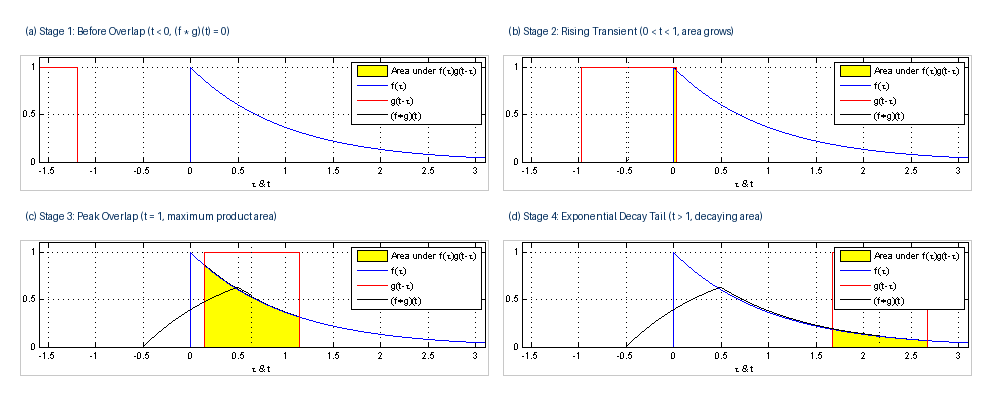
\includegraphics[width=\linewidth]{figures/wikipedia_convolution_animation.png}
\caption{Continuous 1D convolution of a spiky signal $f(\tau)$ with a symmetric box kernel $g(\tau)$ over displacement $t$, illustrating the four mechanical phases: (a) Stage 1: Before Overlap ($t < 0$), where the disjoint supports yield $(f * g)(t) = 0$; (b) Stage 2: Rising Transient ($0 \le t \le 1$), where the leading edge sweeps across the spiky signal and the overlapping area grows; (c) Stage 3: Peak Overlap ($t = 1$), where maximal mass of the spiky signal is contained inside the kernel window, maximizing the integral; (d) Stage 4: Exponential Decay Tail ($t > 1$), where the lagging edge leaves the spiky peak and the integral decays asymptotically. Source: Wikimedia Commons (\href{https://commons.wikimedia.org/wiki/File:Convolution_of_spiky_function_with_box2.gif}{Convolution of spiky function with box2.gif}).}
\label{fig:wikipedia_convolution_animation}
\end{figure}

\paragraph{Continuous 2D Convolution and Algebraic Properties.}
Extending this formulation to continuous 2D functional spaces (such as continuous optical wavefields $\R^2 \to \R$), continuous 2D convolution integrates over both spatial dimensions:
\begin{equation}
S(x, y) = (I * K)(x, y) \triangleq \int_{-\infty}^{\infty} \int_{-\infty}^{\infty} I(\tau_x, \tau_y) K(x - \tau_x, \, y - \tau_y) \, d\tau_x \, d\tau_y.
\label{eq:continuous_2d_convolution}
\end{equation}
Continuous convolution satisfies three foundational algebraic properties:
\begin{itemize}[leftmargin=*]
  \item \textbf{Commutativity}: $f * g = g * f$. By performing the change of variables $u = t - \tau$ (hence $du = -d\tau$):
    \begin{equation}
    (f * g)(t) = \int_{-\infty}^{\infty} f(\tau) g(t - \tau) \, d\tau = \int_{\infty}^{-\infty} f(t - u) g(u) (-du) = \int_{-\infty}^{\infty} g(u) f(t - u) \, du = (g * f)(t).
    \label{eq:convolution_commutativity_proof}
    \end{equation}
  \item \textbf{Associativity}: $f * (g * h) = (f * g) * h$. Cascading linear time-invariant filters can be collapsed into a single equivalent filter $k = g * h$.
  \item \textbf{Distributivity}: $f * (g + h) = (f * g) + (f * h)$.
\end{itemize}

\paragraph{Discrete 2D Cross-Correlation in Deep Learning.}
In computer vision, digital images are discrete 2D matrices of sampled pixel intensities $\mathbf{I} \in \R^{H \times W}$, and filters are discrete 2D tensors $\mathbf{K} \in \R^{F \times F}$. Replacing the continuous integrals with discrete summations, the formal mathematical discrete convolution is:
\begin{equation}
S(i, j) = (\mathbf{I} * \mathbf{K})(i, j) \triangleq \sum_{m=-\infty}^{\infty} \sum_{n=-\infty}^{\infty} \mathbf{I}(m, n) \, \mathbf{K}(i - m, \, j - n).
\label{eq:discrete_convolution_true}
\end{equation}
Because the sum is commutative, Equation~\eqref{eq:discrete_convolution_true} can be equivalently evaluated by flipping the kernel indices:
\begin{equation}
S(i, j) = (\mathbf{K} * \mathbf{I})(i, j) = \sum_{m} \sum_{n} \mathbf{I}(i - m, \, j - n) \, \mathbf{K}(m, n).
\end{equation}
However, modern deep learning libraries (PyTorch, TensorFlow, JAX) do \textbf{not} flip the kernel prior to shifting. Instead, they implement \textbf{discrete 2D cross-correlation}~\cite{bishop2024deep,goodfellow2016deep}:
\begin{equation}
S(i, j) = (\mathbf{I} \star \mathbf{K})(i, j) \triangleq \sum_{m=0}^{F-1} \sum_{n=0}^{F-1} \mathbf{I}(i + m, \, j + n) \, \mathbf{K}(m, n).
\label{eq:discrete_cross_correlation}
\end{equation}
Why do deep learning practitioners universally call cross-correlation ``convolution''? In classical signal processing, filters (such as Sobel or Gaussian filters) are fixed handcrafted mathematical formulas derived in the frequency domain, where commutativity is required for mathematical proofs. In deep learning, however, the kernel weights $\mathbf{K}(m, n)$ are \textbf{free learnable parameters} initialized randomly and updated via backpropagation. If the network needs a flipped filter to minimize the loss $\mathcal{L}$, the optimization algorithm (SGD, Adam) simply learns the reflected parameter values directly! Mathematically:
\begin{equation}
\min_{\mathbf{K}} \mathcal{L}(\mathbf{I} * \mathbf{K}) \equiv \min_{\mathbf{K}'} \mathcal{L}(\mathbf{I} \star \mathbf{K}'), \quad \text{where } \mathbf{K}'(m, n) = \mathbf{K}(-m, -n).
\end{equation}
Omitting the reflection operation saves valuable memory index-shuffling operations on GPUs with exactly zero loss in representational capacity. By convention throughout deep learning, Equation~\eqref{eq:discrete_cross_correlation} is referred to as convolution.

\paragraph{Toeplitz and Circulant Matrix Formulation.}
To reveal the linear algebraic equivalence between convolution and dense layers, consider a 1D discrete input signal $\mathbf{x} = [x_1, x_2, \dots, x_N]^\top \in \R^N$ convolved with a 1D kernel $\mathbf{k} = [k_1, k_2, k_3]^\top \in \R^3$ with zero padding. The 1D convolution can be written strictly as a matrix-vector product $\mathbf{y} = \mathbf{T} \mathbf{x}$, where $\mathbf{T}$ is a \textbf{banded Toeplitz matrix}:
\begin{equation}
\begin{bmatrix}
y_1 \\ y_2 \\ y_3 \\ \vdots \\ y_N
\end{bmatrix}
=
\begin{bmatrix}
k_2 & k_3 & 0 & \dots & 0 \\
k_1 & k_2 & k_3 & \dots & 0 \\
0 & k_1 & k_2 & \ddots & 0 \\
\vdots & \vdots & \ddots & \ddots & k_3 \\
0 & 0 & \dots & k_1 & k_2
\end{bmatrix}
\begin{bmatrix}
x_1 \\ x_2 \\ x_3 \\ \vdots \\ x_N
\end{bmatrix}.
\label{eq:toeplitz_convolution_matrix}
\end{equation}
A Toeplitz matrix has the defining property that each descending diagonal from left to right is constant: $T_{i, j} = T_{i+1, j+1}$. If circular boundary conditions (periodic padding) are imposed, $\mathbf{T}$ becomes a \textbf{Circulant matrix}. Every circulant matrix is fundamentally diagonalized by the Discrete Fourier Transform (DFT) basis matrix $\mathbf{F}$, which provides the algebraic proof of the \textbf{Convolution Theorem}:
\begin{equation}
\mathbf{y} = \mathbf{T} \mathbf{x} \iff \mathcal{F}(\mathbf{y}) = \mathcal{F}(\mathbf{k}) \odot \mathcal{F}(\mathbf{x}),
\label{eq:convolution_theorem}
\end{equation}
where $\odot$ denotes element-wise Hadamard multiplication. This matrix view exposes convolution as a highly structured, constrained linear operator whose weight matrix possesses two defining properties: extreme sparsity and constant diagonals (tied weights).

\begin{figure}[H]
\centering
\begin{tikzpicture}[scale=0.92]
  % Top: Dense Connectivity
  \begin{scope}[shift={(0,3.6)}]
    \node[font=\footnotesize\bfseries\color{politoNavy}] at (2.5, 1.2) {(a) Dense Connectivity (Independent Weights: $5 \times 5 = 25$)};
    \foreach \i in {1,...,5} {
      \node[circle, draw=deepblue, fill=deepblue!15, inner sep=2pt, font=\scriptsize] (in_\i) at (\i, 0) {$x_\i$};
      \node[circle, draw=politoNavy, fill=politoNavy!15, inner sep=2pt, font=\scriptsize] (out_\i) at (\i, -1.5) {$y_\i$};
    }
    \foreach \i in {1,...,5} {
      \foreach \j in {1,...,5} {
        \draw[gray!30, thin] (in_\i) -- (out_\j);
      }
    }
  \end{scope}

  % Bottom: Convolutional Sparse Interactions & Tied Weights
  \begin{scope}[shift={(0,0)}]
    \node[font=\footnotesize\bfseries\color{intuitiongreen}] at (2.5, 0.9) {(b) Convolutional Sparse Interactions (Kernel Size $F=3$, Tied Weights: $3$)};
    \foreach \i in {1,...,5} {
      \node[circle, draw=deepblue, fill=deepblue!15, inner sep=2pt, font=\scriptsize] (cin_\i) at (\i, 0) {$x_\i$};
    }
    \foreach \j in {2,3,4} {
      \node[circle, draw=intuitiongreen, fill=intuitiongreen!20, very thick, inner sep=2pt, font=\scriptsize] (cout_\j) at (\j, -1.5) {$y_\j$};
    }

    % Shared weights color coded
    % Kernel: k_1 (red), k_2 (green), k_3 (blue)
    \foreach \j in {2,3,4} {
      \pgfmathtruncatemacro{\leftin}{\j-1}
      \pgfmathtruncatemacro{\midin}{\j}
      \pgfmathtruncatemacro{\rightin}{\j+1}
      \draw[-{Stealth}, very thick, examred] (cin_\leftin) -- (cout_\j);
      \draw[-{Stealth}, very thick, intuitiongreen] (cin_\midin) -- (cout_\j);
      \draw[-{Stealth}, very thick, politoNavy] (cin_\rightin) -- (cout_\j);
    }

    \node[font=\scriptsize, align=center] at (6.8, -0.7) {
      \textcolor{examred}{$\mathbf{w}_1$ (Left Tap)}\\
      \textcolor{intuitiongreen}{$\mathbf{w}_2$ (Center Tap)}\\
      \textcolor{politoNavy}{$\mathbf{w}_3$ (Right Tap)}
    };
  \end{scope}
\end{tikzpicture}
\caption{Sparse interactions and parameter sharing in convolutional layers compared to dense layers. (a) A dense layer connects every input unit to every output unit with $25$ independent weights. (b) A convolutional layer connects each output unit only to a local spatial receptive field of size $F=3$. The identical weights (color-coded red, green, blue) are reused across all spatial positions.}
\label{fig:sparse_vs_dense_connectivity}
\end{figure}

As shown in Figure~\ref{fig:sparse_vs_dense_connectivity}, discrete convolution mathematically enforces sparse connectivity and parameter sharing. The number of parameters is \textbf{completely independent of image resolution}, determined strictly by kernel size $F \times F \times C$.

\section{CNNs as an infinitely strong spatial prior and biological foundations}
\label{sec:cnns_as_infinitely_strong_prior}

\subsection{The three foundational motivations of CNNs: Sparse interactions, parameter sharing, and equivariant representations}
\label{sec:translation_equivariance_sample_complexity}

In their foundational treatise \textit{Deep Learning}, Ian Goodfellow, Yoshua Bengio, and Aaron Courville~\cite{goodfellow2016deep} establish that convolutional networks improve upon traditional dense feedforward neural architectures by operationalizing three fundamental mathematical ideas: \textbf{sparse interactions} (sparse connectivity), \textbf{parameter sharing} (tied weights), and \textbf{equivariant representations}. We analyze each principle in depth, examine how convolutional architectures algebraically guarantee it, evaluate its practical computational and statistical utility, and formalize why dense Multi-Layer Perceptrons (MLPs) suffer from catastrophic sample complexity on visual data~\cite{goodfellow2016deep,prince2023understanding}.

\paragraph{1. Sparse Interactions (Sparse Connectivity).}
Traditional feedforward neural network layers compute representations using unconstrained matrix multiplication:
\begin{equation}
\mathbf{y} = \sigma(\mathbf{W} \mathbf{x} + \mathbf{b}),
\end{equation}
where every individual output unit interacts with every single input unit via an independent weight parameter $W_{i, j}$. If the input has $m$ units and the output has $n$ units, the transformation requires computing and storing an $n \times m$ matrix, with computational runtime scaling as $\mathcal{O}(m \times n)$.

In stark contrast, Convolutional Neural Networks guarantee \textbf{sparse interactions} (also referred to as \textit{sparse connectivity} or \textit{sparse weights}) by restricting the filter kernel size $F$ to be orders of magnitude smaller than the input spatial dimensions ($F \ll H, W$). Rather than connecting an output unit to all $H \times W$ input pixels, each output unit connects exclusively to a local contiguous receptive field of $F \times F$ pixels (or $F$ taps in 1D). As formalized in the Toeplitz matrix formulation (Equation~\eqref{eq:toeplitz_convolution_matrix}), this restricts non-zero entries in the equivalent transformation matrix strictly to a narrow band of width $F$.

\subparagraph{Receptive Field Deepening.}
Crucially, although direct connections at each individual convolutional layer are strictly sparse, units in deeper layers of a multi-layer CNN interact indirectly with a much larger portion of the input visual grid. As illustrated in Figure~\ref{fig:receptive_field_expansion} later in this chapter, if each layer uses a $1\text{D}$ filter of width $F=3$, a unit in layer $l=1$ observes $3$ input units, a unit in layer $l=2$ observes $5$ input units, and a unit in layer $l$ observes:
\begin{equation}
\text{ERF}_l = l(F - 1) + 1
\end{equation}
input units. By stacking multiple sparsely connected convolutional layers, a deep network allows high-level neurons to synthesize complex, non-local semantic relationships across the entire image canvas while keeping every individual layer's computation strictly localized and memory-efficient.

\subparagraph{Bengio's Edge-Detection Computational Comparison.}
To demonstrate the profound computational advantage of sparse interactions, Goodfellow, Bengio, and Courville~\cite{goodfellow2016deep} provide a canonical quantitative benchmark: detecting edges in a modest digital image of size $320 \times 280$ pixels ($m = 320$, $n = 280$), totaling $D = 320 \times 280 = 89,600$ pixels. Suppose we wish to compute an output feature map of equivalent spatial dimensions ($89,600$ output units).
\begin{itemize}[leftmargin=*]
  \item \textbf{Dense Fully Connected Layer}:
    An unconstrained dense weight matrix $\mathbf{W} \in \R^{89,600 \times 89,600}$ requires storing:
    \begin{equation}
    |\mathbf{W}| = (320 \times 280) \times (320 \times 280) \approx 8.028 \times 10^9 \text{ parameters } (>8 \text{ billion entries}).
    \end{equation}
    In standard 32-bit floating point precision ($4$ bytes per float), storing $\mathbf{W}$ requires:
    \begin{equation}
    8.028 \times 10^9 \times 4\text{ bytes} \approx 32.11 \times 10^9\text{ bytes} \approx 32.1\text{ GB of RAM},
    \end{equation}
    just to store the parameters of a \textit{single} layer, far exceeding the memory bandwidth of high-performance GPUs. Furthermore, evaluating the matrix-vector multiplication requires:
    \begin{equation}
    2 \times (89,600)^2 \approx 1.606 \times 10^{10} \text{ FLOPs } (\approx 16 \text{ billion operations}).
    \end{equation}
  
  \item \textbf{Convolutional Kernel Layer}:
    Now consider performing edge detection using a compact 2-element difference kernel $\mathbf{k} = [-1, 1]^\top$ (or a $2 \times 2$ discrete Sobel-like kernel). The number of parameters to store is strictly:
    \begin{equation}
    |\mathbf{k}| = 2 \text{ parameters } (8\text{ bytes}).
    \end{equation}
    Evaluating the convolution across all $(320 - 1) \times 280 = 89,320$ valid output positions requires:
    \begin{equation}
    89,320 \times 2 \approx 1.786 \times 10^5 \text{ FLOPs } (\approx 2.68 \times 10^5 \text{ FLOPs including bias additions}).
    \end{equation}
\end{itemize}
Comparing the two implementations reveals that the convolutional approach is over \textbf{$60,000$ times faster} computationally and requires over \textbf{$4$ billion times less parameter storage}!

\paragraph{2. Parameter Sharing (Tied Weights).}
The second foundational principle articulated by Bengio is \textbf{parameter sharing} (also known as \textit{tied weights}): using the exact same parameter value across multiple spatial positions in a network. In a conventional dense MLP, each element $W_{i, j}$ of the weight matrix is used exactly once when multiplying the $j$-th input unit to compute the $i$-th output unit. In a CNN, each element of the filter kernel $\mathbf{K} \in \R^{F \times F}$ is applied across \textit{every single receptive field} throughout the entire input grid.

\subparagraph{Memory and Statistical Efficiency.}
While parameter sharing does not change the runtime scaling of forward propagation ($\mathcal{O}(k \times n)$ operations are still performed across the spatial grid), it dramatically reduces the number of unique parameters that must be stored in memory to $O(F^2)$ per input-output channel pair. 

Crucially, parameter sharing provides an enormous boost in \textbf{statistical efficiency}. In a dense MLP, a weight connecting to pixel $(10, 10)$ only learns from patterns presented at pixel $(10, 10)$ during training. If a visual feature (such as a feline eye or a vertical edge) appears at coordinate $(200, 200)$, the weights at $(10, 10)$ receive identically zero gradient feedback. In a CNN, because the filter $\mathbf{K}$ is shared across all spatial coordinates, every pixel patch across every training image contributes a gradient update to the exact same parameter tensor. If an input image contains $100 \times 100 = 10,000$ receptive fields, a single image provides $10,000$ distinct gradient signals to update $\mathbf{K}$, dramatically slashing the number of training samples required to learn robust feature detectors.

\paragraph{3. Equivariant Representations and Transformation Symmetries.}
The third foundational motivation of CNNs is the emergence of \textbf{equivariant representations}. Formally, a mathematical mapping $f$ is said to be \textbf{equivariant} to a transformation $g$ if:
\begin{equation}
f(g(x)) = g(f(x)).
\label{eq:equivariance_general_definition}
\end{equation}
That is, applying the transformation $g$ to the input $x$ and then evaluating $f$ produces the identical result as evaluating $f$ first and then applying $g$ to the representation.

\subparagraph{Invariance vs. Equivariance.}
As formalized by Prince~\cite{prince2023understanding}, visual perception imposes two distinct transformation symmetries that must not be conflated:
\begin{enumerate}[leftmargin=*]
  \item \textbf{Translation Invariance}: A mapping $f: \mathcal{X} \to \mathcal{Y}$ is translation-invariant under spatial shift $\mathcal{T}_{\boldsymbol{\delta}}$ if:
    \begin{equation}
    f\left( \mathcal{T}_{\boldsymbol{\delta}} \mathbf{X} \right) = f(\mathbf{X}), \quad \forall \boldsymbol{\delta} = (\Delta x, \Delta y) \in \mathbb{Z}^2.
    \label{eq:translation_invariance_math}
    \end{equation}
    Translation invariance is the mathematically required property for whole-image categorical classification: whether an object sits in the top-left or bottom-right corner of the canvas, its semantic category label (\textit{``Cat''}) must remain unchanged.
  
  \item \textbf{Translation Equivariance (Covariance)}: A mapping $f: \mathcal{X} \to \mathcal{Z}$ is translation-equivariant under spatial shift $\mathcal{T}_{\boldsymbol{\delta}}$ if:
    \begin{equation}
    f\left( \mathcal{T}_{\boldsymbol{\delta}} \mathbf{X} \right) = \mathcal{T}_{\boldsymbol{\delta}} \big[ f(\mathbf{X}) \big], \quad \forall \boldsymbol{\delta} \in \mathbb{Z}^2.
    \label{eq:translation_equivariance_math}
    \end{equation}
    Translation equivariance is the indispensable property for internal feature representations, dense localization, and semantic segmentation: if an object moves three pixels to the right in the visual field, all extracted feature activations in the convolutional feature map must shift by exactly three pixels to preserve physical spatial geometry.
\end{enumerate}

\subparagraph{Bengio's Caveat: When NOT to Share Parameters.}
Goodfellow, Bengio, and Courville~\cite{goodfellow2016deep} highlight a critical architectural caveat: \textit{parameter sharing across space is beneficial if and only if the underlying data-generating distribution is spatially stationary}---that is, when features useful at one location are equally useful at all other locations. While this assumption holds universally for unconstrained natural images, it is \textbf{fundamentally suboptimal} when images possess a fixed, canonical spatial composition.
\begin{itemize}[leftmargin=*]
  \item \textbf{The Canonical Example of Aligned Faces}:
    Consider a biometric dataset of tightly cropped, pre-aligned human faces (e.g., LFW or CelebA). In these images, eyes are consistently positioned in the upper quadrant, noses reside in the center, and mouths are located in the lower quadrant. There is zero reason to search for an eye in the bottom corner or a mouth at the top of the canvas!
  \item \textbf{The Unshared Locally Connected Solution}:
    Forced weight sharing across the entire grid forces the network to compromise between detecting eyes and detecting mouths using the same shared filters. In such canonically framed domains, \textbf{unshared locally connected layers} (also known as tiled convolutions without weight sharing) are theoretically and empirically superior: connections remain spatially localized to $F \times F$ patches (preserving sparse interactions), but different spatial positions $(i, j)$ learn completely separate, decoupled weight matrices $\mathbf{K}_{(i, j)}$.
\end{itemize}

\paragraph{The Catastrophic Sample Complexity of Dense MLPs.}
To understand why parameter sharing and translation equivariance cannot simply be learned by dense MLPs, consider an MLP processing a flattened image vector $\mathbf{x} = \operatorname{vec}(\mathbf{X}) \in \R^{D}$ with $D = H \cdot W$. A fully connected layer computes hidden activations via an unconstrained dense weight matrix $\mathbf{W} \in \R^{D_{\text{out}} \times D}$:
\begin{equation}
h_p = \sigma\left( \sum_{i=1}^H \sum_{j=1}^W W_{p, (i, j)} X_{i, j} + b_p \right).
\label{eq:mlp_dense_coordinate_dot}
\end{equation}
Notice that in Equation~\eqref{eq:mlp_dense_coordinate_dot}, every input coordinate $(i, j)$ is governed by a completely independent, decoupled parameter $W_{p, (i, j)}$.

Suppose a visual pattern $\mathcal{P}$ (e.g., an eye or a sharp vertical edge) is presented at spatial coordinate $(i_1, j_1)$ during training. Backpropagation calculates the gradient of the objective $\mathcal{L}$ with respect to the weights connected to that specific coordinate:
\begin{equation}
\frac{\partial \mathcal{L}}{\partial W_{p, (i_1, j_1)}} = \delta_p X_{i_1, j_1} \neq 0.
\end{equation}
However, for any other spatial coordinate $(i_2, j_2) \neq (i_1, j_1)$ where the pattern was not presented, the local input is zero or background, yielding:
\begin{equation}
\frac{\partial \mathcal{L}}{\partial W_{p, (i_2, j_2)}} = 0.
\end{equation}
The weights connected to coordinate $(i_2, j_2)$ receive \textbf{identically zero gradient updates}! Consequently, if the object appears at position $(i_2, j_2)$ at test time, the MLP possesses zero ability to recognize it.

To learn translation equivariance empirically, the MLP must observe every visual concept $\mathcal{P}$ instantiated at every coordinate in the spatial translation group $\mathcal{T} = \{(\Delta x, \Delta y) \mid 0 \le \Delta x < W, \, 0 \le \Delta y < H\}$. Because the cardinality of this group is $|\mathcal{T}| = H \times W$, the required training sample complexity scales as:
\begin{equation}
N_{\text{MLP}} = \Omega\left( |\mathcal{T}| \cdot N_0 \right) = \Omega\left( H \cdot W \cdot N_0 \right),
\label{eq:sample_complexity_mlp}
\end{equation}
where $N_0$ is the sample complexity required to learn the pattern at a single fixed location. For a standard $256 \times 256$ input image, $|\mathcal{T}| = 65,536$: an MLP requires up to a \textbf{$65,000\times$ larger dataset} purely to brute-force learn translation invariance through exhaustive spatial data augmentation!

\begin{figure}[H]
\centering
\begin{tikzpicture}[scale=0.90]
  % -------------------------------------------------------------
  % PANEL (a): MLP Failure & High Sample Complexity
  % -------------------------------------------------------------
  \node[font=\footnotesize\bfseries, text=examred, align=center] at (2.6, 3.6) {
    (a) Dense Multi-Layer Perceptron\\[2pt]
    {\scriptsize\normalfont\color{examred!90!black}Spatial Decoupling: $\Omega(H \cdot W \cdot N_0)$}
  };
  
  % Input Grid 1 (Pattern at Top-Left)
  \draw[fill=gray!12, draw=gray!50, rounded corners=1pt] (0.4, 1.2) rectangle (1.8, 2.6);
  \draw[step=0.35, gray!25, thin] (0.4, 1.2) grid (1.8, 2.6);
  \node[fill=examred!25, draw=examred, thick, rounded corners=1pt, inner sep=1.8pt, font=\tiny\bfseries\color{examred}] at (0.58, 2.42) {Obj};
  \node[font=\tiny, text=gray!80, anchor=north] at (1.1, 1.05) {Position $(i_1, j_1)$};

  % MLP Layer 1 (Hidden Neuron h1)
  \node[circle, draw=politoNavy, fill=politoNavy!15, thick, inner sep=2.5pt, font=\scriptsize\bfseries\color{politoNavy}] (h1) at (5.0, 1.9) {$h_1$};
  \draw[-{Stealth[scale=1.0]}, thick, examred] (1.85, 2.1) -- (h1) 
    node[midway, above=2pt, font=\tiny\bfseries, text=examred] {$\mathbf{w}_1$ (Learned)};

  % Input Grid 2 (Pattern Shifted to Bottom-Right)
  \draw[fill=gray!12, draw=gray!50, rounded corners=1pt] (0.4, -0.8) rectangle (1.8, 0.6);
  \draw[step=0.35, gray!25, thin] (0.4, -0.8) grid (1.8, 0.6);
  \node[fill=deepblue!25, draw=deepblue, thick, rounded corners=1pt, inner sep=1.8pt, font=\tiny\bfseries\color{deepblue}] at (1.62, -0.42) {Obj};
  \node[font=\tiny, text=gray!80, anchor=north] at (1.1, -0.95) {Position $(i_2, j_2)$};

  % MLP Layer 2 (Hidden Neuron h2)
  \node[circle, draw=politoNavy, fill=politoNavy!15, thick, inner sep=2.5pt, font=\scriptsize\bfseries\color{politoNavy}] (h2) at (5.0, -0.1) {$h_2$};
  \draw[-{Stealth[scale=1.0]}, thick, dashed, gray!60] (1.85, -0.3) -- (h2) 
    node[midway, above=2pt, font=\tiny\bfseries, text=gray!70] {$\mathbf{w}_2$ (Untrained!)};

  % Panel (a) Consequence Callout Box (Narrower with ample margins)
  \node[draw=examred!50, fill=examback, rounded corners=2pt, inner sep=3.5pt, align=center, font=\tiny, text=examred!90!black] at (2.6, -1.95) {
    $\implies$ Requires observing pattern at all $H \times W$ locations\\
    $\partial \mathcal{L} / \partial W_{p,(i_2, j_2)} = 0 \implies$ Zero transfer across space
  };

  % -------------------------------------------------------------
  % CENTRAL DIVIDER
  % -------------------------------------------------------------
  \draw[dashed, gray!40, thick] (5.9, -2.4) -- (5.9, 3.9);

  % -------------------------------------------------------------
  % PANEL (b): CNN Weight Tying & Exact Equivariance
  % -------------------------------------------------------------
  \node[font=\footnotesize\bfseries, text=intuitiongreen, align=center] at (9.4, 3.6) {
    (b) Convolutional Neural Network\\[2pt]
    {\scriptsize\normalfont\color{intuitiongreen!90!black}Shift Equivariance: $O(N_0)$ samples}
  };

  % Conv input with pattern at Top-Left
  \draw[fill=gray!12, draw=gray!50, rounded corners=1pt] (6.6, 1.2) rectangle (8.0, 2.6);
  \draw[step=0.35, gray!25, thin] (6.6, 1.2) grid (8.0, 2.6);
  \node[fill=examred!25, draw=examred, thick, rounded corners=1pt, inner sep=1.8pt, font=\tiny\bfseries\color{examred}] at (6.78, 2.42) {Obj};
  \node[font=\tiny, text=gray!80, anchor=north] at (7.3, 1.05) {Position $(i_1, j_1)$};

  % Conv output map 1
  \draw[fill=intuitiongreen!10, draw=intuitiongreen!80, rounded corners=1pt] (10.8, 1.2) rectangle (12.2, 2.6);
  \draw[step=0.35, intuitiongreen!20, thin] (10.8, 1.2) grid (12.2, 2.6);
  \node[fill=intuitiongreen!40, draw=intuitiongreen, thick, rounded corners=1pt, inner sep=1.8pt, font=\tiny\bfseries, text=intuitiongreen!90!black] at (10.98, 2.42) {Act};
  \node[font=\tiny, text=gray!80, anchor=north] at (11.5, 1.05) {Response at $(i_1, j_1)$};

  \draw[-{Stealth[scale=1.0]}, thick, intuitiongreen] (8.2, 1.9) -- (10.6, 1.9) 
    node[midway, above=2pt, font=\tiny\bfseries, text=intuitiongreen] {Kernel $\mathbf{K}$};

  % Conv input with pattern shifted to Bottom-Right
  \draw[fill=gray!12, draw=gray!50, rounded corners=1pt] (6.6, -0.8) rectangle (8.0, 0.6);
  \draw[step=0.35, gray!25, thin] (6.6, -0.8) grid (8.0, 0.6);
  \node[fill=deepblue!25, draw=deepblue, thick, rounded corners=1pt, inner sep=1.8pt, font=\tiny\bfseries\color{deepblue}] at (7.82, -0.42) {Obj};
  \node[font=\tiny, text=gray!80, anchor=north] at (7.3, -0.95) {Position $(i_2, j_2)$};

  % Conv output map 2
  \draw[fill=intuitiongreen!10, draw=intuitiongreen!80, rounded corners=1pt] (10.8, -0.8) rectangle (12.2, 0.6);
  \draw[step=0.35, intuitiongreen!20, thin] (10.8, -0.8) grid (12.2, 0.6);
  \node[fill=intuitiongreen!40, draw=intuitiongreen, thick, rounded corners=1pt, inner sep=1.8pt, font=\tiny\bfseries, text=intuitiongreen!90!black] at (12.02, -0.42) {Act};
  \node[font=\tiny, text=gray!80, anchor=north] at (11.5, -0.95) {Response at $(i_2, j_2)$};

  \draw[-{Stealth[scale=1.0]}, thick, intuitiongreen] (8.2, -0.1) -- (10.6, -0.1) 
    node[midway, above=2pt, font=\tiny\bfseries, text=intuitiongreen] {Same $\mathbf{K}$!};

  % Panel (b) Consequence Callout Box (Narrower with ample margins)
  \node[draw=intuitiongreen!50, fill=intuitionback, rounded corners=2pt, inner sep=3.5pt, align=center, font=\tiny, text=intuitiongreen!90!black] at (9.4, -1.95) {
    $\implies$ Exact translation equivariance: $f(\mathcal{T}_{\boldsymbol{\delta}}\mathbf{X}) = \mathcal{T}_{\boldsymbol{\delta}}[f(\mathbf{X})]$\\
    Sample complexity $O(N_0)$ independent of grid size
  };
\end{tikzpicture}
\caption{Sample complexity contrast between dense MLPs and Convolutional Networks under 2D spatial translation. (a) In an MLP, disjoint weights connect to each spatial pixel; learning a visual concept at position $(i_1, j_1)$ fails to generalize to position $(i_2, j_2)$. (b) In a CNN, parameter sharing ties all spatial positions to identical kernel weights $\mathbf{K}$, guaranteeing exact translation equivariance and sample complexity scaling independent of grid resolution.}
\label{fig:mlp_vs_cnn_sample_complexity}
\end{figure}

\paragraph{The CNN Algebraic Inductive Bias.}
As illustrated in Figure~\ref{fig:mlp_vs_cnn_sample_complexity}, a Convolutional Neural Network resolves this dilemma by hardcoding translation equivariance directly into its algebraic structure through \textbf{parameter sharing (tied weights)}. Convolving input $\mathbf{X}$ with shared kernel $\mathbf{K} \in \R^{F \times F}$ guarantees commutativity with translation by algebraic identity:
\begin{equation}
\begin{aligned}
\big[ (\mathcal{T}_{\boldsymbol{\delta}} \mathbf{X}) * \mathbf{K} \big](i, j) &= \sum_{m=0}^{F-1} \sum_{n=0}^{F-1} (\mathcal{T}_{\boldsymbol{\delta}} \mathbf{X})(i+m, \, j+n) \, K_{m, n} \\
&= \sum_{m=0}^{F-1} \sum_{n=0}^{F-1} \mathbf{X}(i - \Delta x + m, \, j - \Delta y + n) \, K_{m, n} \\
&= (\mathbf{X} * \mathbf{K})(i - \Delta x, \, j - \Delta y) = \mathcal{T}_{\boldsymbol{\delta}} \big[ (\mathbf{X} * \mathbf{K}) \big](i, j).
\end{aligned}
\label{eq:equivariance_proof}
\end{equation}
Because Equation~\eqref{eq:equivariance_proof} holds for \textit{any} kernel values $\mathbf{K}$, translation equivariance is strictly hardcoded prior to observing any training data. Observing a visual feature at a single location $(i_1, j_1)$ produces a gradient that updates the shared kernel $\mathbf{K}$; this single parameter update immediately generalizes detection across all $H \times W$ locations simultaneously:
\begin{equation}
N_{\text{CNN}} = O(N_0).
\label{eq:sample_complexity_cnn}
\end{equation}
As Simon Prince highlights~\cite{prince2023understanding}, weight sharing acts as an \textbf{infinite Bayesian prior} (or Dirac delta regularization) that penalizes all non-translation-equivariant linear mappings to infinity, slashing hypothesis complexity without sacrificing expressive power.

\subsection{Biological visual cortex foundations and spontaneous Gabor emergence}
\label{sec:biological_visual_cortex_and_gabor_emergence}

The hierarchical design of Convolutional Neural Networks is deeply rooted in 20th-century neurobiology, reflecting profound mathematical parallels between mammalian visual processing and statistical gradient optimization~\cite{bishop2024deep}.

\paragraph{1. The Hubel \& Wiesel Discovery (1959, 1962).}
In their Nobel-Prize-winning electrophysiological investigations, David Hubel and Torsten Wiesel recorded action potentials from individual cortical neurons in the feline striate cortex (primary visual cortex, Area 17 / V1) under controlled visual illumination~\cite{hubel1959receptive,hubel1962receptive}. They established that cortical neurons do not respond to uniform, diffuse illumination. Instead, V1 visual processing is organized hierarchically:
\begin{enumerate}[leftmargin=*]
  \item \textbf{Simple Cells}: Simple cells possess spatially localized receptive fields partitioned into antagonistic excitatory (ON) and inhibitory (OFF) sub-regions. They fire vigorously only in response to oriented visual stimuli (slits, bars, or sharp edges) oriented at a specific angle $\theta$ and situated at a precise spatial location $(x_0, y_0)$ in the visual field.
  \item \textbf{Complex Cells}: Deeper within the cortical lamina, complex cells receive convergent inputs from groups of simple cells sharing identical orientation preferences $\theta$ across adjacent spatial positions. Complex cells respond to oriented edges anywhere within a broader receptive field, displaying \textbf{local translation invariance} to small spatial shifts.
\end{enumerate}
This functional division---simple cells detecting localized oriented features followed by complex cells pooling across space---provided the direct biological archetype for Fukushima's \textit{Neocognitron} (1980)~\cite{fukushima1980neocognitron} and LeCun's \textit{LeNet} (1989, 1998)~\cite{lecun1989backpropagation,lecun1998gradient}: \textbf{convolutional layers computationally embody simple cells, while pooling layers embody complex cells}.

\paragraph{2. Mathematical Modeling: 2D Gabor Wavelets.}
Subsequent neurophysiological mapping (Daugman, 1985; Jones \& Palmer, 1987) demonstrated that the spatial receptive field response profile of a V1 simple cell is modeled with exceptional mathematical precision by a \textbf{2D Gabor filter}~\cite{bishop2024deep}: a 2D sinusoidal plane wave modulated by an anisotropic Gaussian decay envelope.

Following Bishop~\cite{bishop2024deep}, the continuous 2D Gabor function $G: \R^2 \to \R$ is defined by:
\begin{equation}
G(x, y) = A \exp\left( -\alpha \tilde{x}^2 - \beta \tilde{y}^2 \right) \sin(\omega \tilde{x} + \phi),
\label{eq:bishop_gabor_formula}
\end{equation}
where $(\tilde{x}, \tilde{y})$ represent coordinates rotated by orientation angle $\theta$ and translated to receptive field center $(x_0, y_0)$:
\begin{align}
\tilde{x} &= (x - x_0) \cos\theta + (y - y_0) \sin\theta, \label{eq:gabor_xtilde} \\
\tilde{y} &= -(x - x_0) \sin\theta + (y - y_0) \cos\theta. \label{eq:gabor_ytilde}
\end{align}
The analytical parameters in Equations~\eqref{eq:bishop_gabor_formula}--\eqref{eq:gabor_ytilde} govern physical feature tuning:
\begin{itemize}[noitemsep]
  \item $\theta \in [0, \pi)$: The preferred orientation angle of the edge detector.
  \item $\omega \in \R_+$: The spatial frequency of the sinusoidal oscillation, tuning the detector to specific edge scales.
  \item $\phi \in [0, 2\pi)$: The phase angle ($\phi = 0$ corresponds to an odd-symmetric, anti-phase edge detector; $\phi = \pi/2$ corresponds to an even-symmetric bar detector).
  \item $\alpha, \beta > 0$: Spatial decay constants determining the Gaussian standard deviations $\sigma_x = 1/\sqrt{2\alpha}$ (across stripes) and $\sigma_y = 1/\sqrt{2\beta}$ (along stripes).
\end{itemize}
In harmonic analysis, 2D Gabor functions possess a remarkable property: they uniquely attain the theoretical lower bound of the \textbf{Heisenberg-Gabor joint uncertainty relation} in space and spatial frequency:
\begin{equation}
\Delta x \cdot \Delta u \ge \frac{1}{4\pi}, \quad \Delta y \cdot \Delta v \ge \frac{1}{4\pi}.
\label{eq:heisenberg_gabor_uncertainty}
\end{equation}
They are the optimal mathematical operators for simultaneously localizing spatial position $(x, y)$ and orientation/frequency $(u, v)$.

\paragraph{3. Spontaneous Gabor Emergence via Backpropagation on Natural Images.}
When a deep convolutional network (such as AlexNet~\cite{krizhevsky2012imagenet} or VGG~\cite{simonyan2014very}) is trained on large-scale datasets (ImageNet) using standard stochastic gradient descent to minimize cross-entropy loss:
\begin{equation}
\min_{\mathbf{W}} \frac{1}{N} \sum_{i=1}^N \mathcal{L}_{\text{CE}}\big( f(\mathbf{X}_i; \mathbf{W}), y_i \big),
\end{equation}
a remarkable phenomenon emerges: \textbf{the first-layer convolutional filters spontaneously organize into oriented Gabor-like wavelets and color-opponent blob filters}~\cite{krizhevsky2012imagenet,bishop2024deep}.

Crucially, \textbf{no biological priors or Gabor templates were engineered into the network or the loss function}. Why does pure gradient descent autonomously rediscover mammalian visual cortex receptive fields?
\begin{itemize}[leftmargin=*]
  \item \textbf{Natural Image Statistics}: As established by Olshausen \& Field (1996)~\cite{olshausen1996emergence} and Bell \& Sejnowski (1997), natural images are not random Gaussian noise; their power spectra follow a universal scale-invariant power law $P(f) \propto 1/f^{2-\eta}$ governed by sharp physical occlusion boundaries. Seeking an optimal, non-redundant sparse code for natural image patches mathematically forces basis functions to converge to localized, oriented bandpass wavelets.
  \item \textbf{Color Opponency}: On 3-channel RGB imagery, early filters spontaneously split into achromatic (luminance) edge detectors and chromatic color-opponent filters: Red vs. Green ($R - G$) and Blue vs. Yellow ($B - (R+G)/2$). Gradient descent spontaneously rediscovers Hering's 1878 \textbf{opponent-process theory of biological color vision}.
\end{itemize}

As Christopher Bishop cautions~\cite{bishop2024deep}, this convergence does not prove that CNNs function as biophysical models of the mammalian brain; rather, it demonstrates that \textbf{Gabor-like filtering and color opponency are universal mathematical solutions dictated by the statistical physics of natural imagery}. Both biological evolution and artificial backpropagation independently discover the exact same optimal representations.

\subsection{Anatomy of a convolutional layer: Stride, padding, and output geometry}
\label{sec:conv_layer_anatomy}

We now formalize the full multi-channel convolutional layer as deployed in modern deep networks.

\paragraph{Input and Filter Tensor Volumes.}
\begin{itemize}
  \item The input is a 3D tensor volume $\mathbf{X} \in \R^{H_{\text{in}} \times W_{\text{in}} \times C_{\text{in}}}$, where $H_{\text{in}}, W_{\text{in}}$ denote spatial height and width, and $C_{\text{in}}$ denotes channel depth (e.g., $C_{\text{in}} = 3$ for RGB color images).
  \item The layer contains a bank of $C_{\text{out}}$ distinct convolutional filters.
  \item \textbf{Fundamental Depth Rule}: \textbf{Each filter kernel must span the ENTIRE depth $C_{\text{in}}$ of the input volume!} A filter has spatial dimensions $F \times F$, but volumetric dimensions:
    \begin{equation}
    \mathbf{K}^{(k)} \in \R^{F \times F \times C_{\text{in}}}, \quad \forall k \in \{1, \dots, C_{\text{out}}\}.
    \end{equation}
\end{itemize}

Each filter kernel $\mathbf{K}^{(k)}$ computes an element-wise dot product across all $C_{\text{in}}$ channels simultaneously over a local spatial window, adds a scalar bias $b_k \in \R$, and emits a single 2D spatial slice $\mathbf{Y}_{:,:,k} \in \R^{H_{\text{out}} \times W_{\text{out}}}$:
\begin{equation}
\mathbf{Y}_{i, j, k} = \sum_{c=1}^{C_{\text{in}}} \sum_{m=0}^{F-1} \sum_{n=0}^{F-1} \mathbf{X}_{i+m, \, j+n, \, c} \, \mathbf{K}^{(k)}_{m, n, c} + b_k.
\label{eq:multichannel_convolution}
\end{equation}
Stacking the resulting $C_{\text{out}}$ 2D feature maps produces the output volume $\mathbf{Y} \in \R^{H_{\text{out}} \times W_{\text{out}} \times C_{\text{out}}}$.

\begin{figure}[H]
\centering
\begin{tikzpicture}[scale=0.95]
  % 3D Input Volume: 32x32x3
  \draw[fill=deepblue!15, draw=deepblue, thick] (0, 0) -- (2.0, 0) -- (2.0, 2.0) -- (0, 2.0) -- cycle;
  \draw[fill=deepblue!25, draw=deepblue, thick] (2.0, 0) -- (2.6, 0.6) -- (2.6, 2.6) -- (2.0, 2.0) -- cycle;
  \draw[fill=deepblue!10, draw=deepblue, thick] (0, 2.0) -- (0.6, 2.6) -- (2.6, 2.6) -- (2.0, 2.0) -- cycle;
  \node[font=\footnotesize\bfseries\color{politoNavy}, align=center] at (1.0, 1.0) {Input Volume\\$32 \times 32 \times 3$};

  % Local filter spanning full depth
  \draw[fill=examred!30, draw=examred, thick] (0.5, 0.7) -- (1.1, 0.7) -- (1.1, 1.3) -- (0.5, 1.3) -- cycle;
  \draw[fill=examred!40, draw=examred, thick] (1.1, 0.7) -- (1.7, 1.3) -- (1.7, 1.9) -- (1.1, 1.3) -- cycle;
  \draw[fill=examred!20, draw=examred, thick] (0.5, 1.3) -- (1.1, 1.9) -- (1.7, 1.9) -- (1.1, 1.3) -- cycle;
  \node[font=\tiny\color{examred}, align=center] at (1.1, 1.3) {$5 \times 5$\\$\times 3$};

  % Filter bank arrow
  \draw[-{Stealth}, very thick, examred] (2.8, 1.3) -- (4.2, 1.3) node[midway, above, font=\scriptsize, align=center] {$6$ Filters\\$5 \times 5 \times 3$};

  % Output Volume: 28x28x6
  \draw[fill=intuitiongreen!15, draw=intuitiongreen, thick] (4.5, 0.2) -- (6.3, 0.2) -- (6.3, 2.0) -- (4.5, 2.0) -- cycle;
  \draw[fill=intuitiongreen!25, draw=intuitiongreen, thick] (6.3, 0.2) -- (7.5, 1.4) -- (7.5, 3.2) -- (6.3, 2.0) -- cycle;
  \draw[fill=intuitiongreen!10, draw=intuitiongreen, thick] (4.5, 2.0) -- (5.7, 3.2) -- (7.5, 3.2) -- (6.3, 2.0) -- cycle;
  \node[font=\footnotesize\bfseries\color{intuitiongreen}, align=center] at (5.4, 1.1) {Output Volume\\$28 \times 28 \times 6$};
\end{tikzpicture}
\caption{The volumetric geometry of multi-channel convolution. An input volume of $32 \times 32 \times 3$ is convolved by $C_{\text{out}} = 6$ distinct filters. Each individual filter spans the complete depth of the input volume ($5 \times 5 \times 3$), emitting a single 2D feature map ($28 \times 28$). Stacking the 6 resulting activation maps produces the output volume of size $28 \times 28 \times 6$.}
\label{fig:volumetric_convolution}
\end{figure}

\paragraph{Hyperparameters: Stride and Padding.}
The spatial dimensions $H_{\text{out}}, W_{\text{out}}$ are governed by three hyperparameters:
\begin{itemize}
  \item \textbf{Filter Size ($F$)}: The spatial extent of the kernel (typically $F \in \{3, 5, 7\}$).
  \item \textbf{Stride ($S$)}: The step size (in pixels) by which the filter shifts across the input grid. A stride of $S = 1$ shifts pixel-by-pixel; a stride of $S = 2$ skips every second pixel, downsampling spatial resolution by a factor of 2.
  \item \textbf{Zero-Padding ($P$)}: The number of zero-valued pixels appended to the perimeter of the input feature map.
\end{itemize}

\begin{theorem}[Universal Spatial Dimension Formula]
Given an input spatial dimension $N_{\text{in}}$ (height or width), filter size $F$, zero-padding $P$, and stride $S$, the output spatial dimension $N_{\text{out}}$ is given by:
\begin{equation}
N_{\text{out}} = \left\lfloor \frac{N_{\text{in}} - F + 2P}{S} \right\rfloor + 1.
\label{eq:spatial_dimension_formula}
\end{equation}
\end{theorem}

\paragraph{Walkthrough of Slide Examples: How Each Hyperparameter Governs Output Size.}
To understand how each hyperparameter component in Equation~\eqref{eq:spatial_dimension_formula} governs the output, consider the visual decomposition in Figure~\ref{fig:conv_hyperparameter_walkthrough}.

\begin{figure}[H]
\centering
\begin{tikzpicture}[scale=0.88]
  % Case 1: N_in = 7, F = 3, P = 0, S = 1 => N_out = 5
  \begin{scope}[shift={(0,3.6)}]
    \node[font=\footnotesize\bfseries\color{politoNavy}] at (3.5, 1.2) {Case 1: $N_{\text{in}}=7, F=3, P=0, S=1 \implies N_{\text{out}} = \frac{7-3+0}{1} + 1 = 5$};
    \foreach \x in {0,...,6} {
      \draw[fill=deepblue!15, draw=deepblue, thick] (\x, 0) rectangle (\x+0.8, 0.8);
      \node[font=\tiny] at (\x+0.4, 0.4) {$\x$};
    }
    % Filter highlight
    \draw[draw=examred, ultra thick, fill=examred!20, opacity=0.6] (0, 0) rectangle (2.8, 0.8);
    \draw[-{Stealth}, thick, examred] (0.4, -0.3) -- (1.4, -0.3) node[midway, below, font=\tiny] {$S=1$};
  \end{scope}

  % Case 2: N_in = 7, F = 3, P = 0, S = 2 => N_out = 3
  \begin{scope}[shift={(0,1.8)}]
    \node[font=\footnotesize\bfseries\color{politoNavy}] at (3.5, 1.2) {Case 2: $N_{\text{in}}=7, F=3, P=0, S=2 \implies N_{\text{out}} = \frac{7-3+0}{2} + 1 = 3$};
    \foreach \x in {0,...,6} {
      \draw[fill=deepblue!15, draw=deepblue, thick] (\x, 0) rectangle (\x+0.8, 0.8);
      \node[font=\tiny] at (\x+0.4, 0.4) {$\x$};
    }
    % Filter highlight step 1
    \draw[draw=examred, ultra thick, fill=examred!20, opacity=0.6] (0, 0) rectangle (2.8, 0.8);
    \draw[-{Stealth}, thick, examred] (0.4, -0.3) -- (2.4, -0.3) node[midway, below, font=\tiny] {$S=2$ (Skips 1 pixel)};
  \end{scope}

  % Case 3: N_in = 7, F = 3, P = 1, S = 1 => "Same" Padding => N_out = 7
  \begin{scope}[shift={(0,0)}]
    \node[font=\footnotesize\bfseries\color{intuitiongreen}] at (3.5, 1.2) {Case 3: $N_{\text{in}}=7, F=3, P=1, S=1 \implies N_{\text{out}} = \frac{7-3+2(1)}{1} + 1 = 7$ ("Same" Padding)};
    % Padding cells (dashed)
    \draw[fill=gray!20, draw=gray!70, dashed, thick] (-1.0, 0) rectangle (-0.2, 0.8);
    \node[font=\tiny\color{gray!70}] at (-0.6, 0.4) {$0$};
    \foreach \x in {0,...,6} {
      \draw[fill=deepblue!15, draw=deepblue, thick] (\x, 0) rectangle (\x+0.8, 0.8);
      \node[font=\tiny] at (\x+0.4, 0.4) {$\x$};
    }
    \draw[fill=gray!20, draw=gray!70, dashed, thick] (7.0, 0) rectangle (7.8, 0.8);
    \node[font=\tiny\color{gray!70}] at (7.4, 0.4) {$0$};

    % Filter over padded border
    \draw[draw=intuitiongreen, ultra thick, fill=intuitiongreen!20, opacity=0.6] (-1.0, 0) rectangle (1.8, 0.8);
  \end{scope}
\end{tikzpicture}
\caption{Visual walkthrough of convolutional spatial dimension mechanics. Top: A $7 \times 7$ grid with $3 \times 3$ filter and stride 1 produces $5 \times 5$. Middle: Stride 2 shifts the kernel by two pixels at a time, skipping every second location to yield $3 \times 3$. Bottom: Adding zero-padding $P = (F-1)/2 = 1$ appends a boundary of zeros, perfectly preserving the original spatial dimension $7 \times 7$ ("Same" padding).}
\label{fig:conv_hyperparameter_walkthrough}
\end{figure}

The mathematical walkthroughs presented by Prof.~Tommasi demonstrate:
\begin{enumerate}
  \item \textbf{Input $7 \times 7$, Filter $3 \times 3$, Stride $S=1$, Padding $P=0$}:
    \begin{equation}
    N_{\text{out}} = \frac{7 - 3 + 2(0)}{1} + 1 = \frac{4}{1} + 1 = 5 \implies \text{Output is } 5 \times 5.
    \end{equation}
  \item \textbf{Input $7 \times 7$, Filter $3 \times 3$, Stride $S=2$, Padding $P=0$}:
    \begin{equation}
    N_{\text{out}} = \frac{7 - 3 + 2(0)}{2} + 1 = \frac{4}{2} + 1 = 3 \implies \text{Output is } 3 \times 3.
    \end{equation}
  \item \textbf{Input $7 \times 7$, Filter $3 \times 3$, Stride $S=3$, Padding $P=0$}:
    \begin{equation}
    \frac{7 - 3 + 0}{3} + 1 = \frac{4}{3} + 1 = 2.33 \implies \text{Fractional! The filter does NOT fit without clipping!}
    \end{equation}
    In valid convolutional designs, hyperparameters must satisfy $(N_{\text{in}} - F + 2P) \pmod S = 0$.
  \item \textbf{Zero-Padding: "Same" vs. "Valid" Padding}:
    Without padding ($P = 0$, "valid" padding), applying an $F \times F$ convolution inevitably shrinks the spatial resolution by $(F - 1)$ pixels at each layer. In deep networks with dozens of layers, the feature map would collapse to $1 \times 1$ within a few layers, destroying spatial context.
    To preserve spatial resolution ($N_{\text{out}} = N_{\text{in}}$ with stride $S = 1$, known as \textbf{"Same" padding}), we set:
    \begin{equation}
    N_{\text{in}} = \frac{N_{\text{in}} - F + 2P}{1} + 1 \implies 2P = F - 1 \implies P = \frac{F - 1}{2}.
    \label{eq:same_padding_formula}
    \end{equation}
    For standard $3 \times 3$ filters ($F = 3$), setting $P = (3-1)/2 = 1$ perfectly maintains spatial dimensions. For $5 \times 5$ filters ($F = 5$), setting $P = 2$ preserves dimensions.
\end{enumerate}

\paragraph{Parameter and FLOP Counting.}
Let a convolutional layer process input $\mathbf{X} \in \R^{H \times W \times C_{\text{in}}}$ with $C_{\text{out}}$ filters of size $F \times F \times C_{\text{in}}$, stride $S$, and padding $P$:
\begin{itemize}
  \item \textbf{Total Learnable Parameters}: Each filter contains $F \times F \times C_{\text{in}}$ kernel weights plus 1 scalar bias. For $C_{\text{out}}$ filters:
    \begin{equation}
    N_{\text{params}} = \left( F \times F \times C_{\text{in}} + 1 \right) \times C_{\text{out}}.
    \label{eq:conv_param_count}
    \end{equation}
    Notice that $N_{\text{params}}$ is completely independent of the spatial size $H, W$!
  \item \textbf{Total Floating-Point Multiply-Accumulate Operations (FLOPs)}: Computing each scalar output activation requires $(F \times F \times C_{\text{in}})$ multiplications and additions. Emitting the full volume $H_{\text{out}} \times W_{\text{out}} \times C_{\text{out}}$ requires:
    \begin{equation}
    N_{\text{FLOPs}} = 2 \times H_{\text{out}} \times W_{\text{out}} \times \left( F \times F \times C_{\text{in}} \right) \times C_{\text{out}}.
    \label{eq:conv_flops_count}
    \end{equation}
\end{itemize}

\begin{example}[Slide Parameter Walkthrough]
Let input volume be $32 \times 32 \times 3$. We apply $C_{\text{out}} = 10$ filters of size $5 \times 5$, with stride $S = 1$ and padding $P = 2$:
\begin{itemize}[noitemsep]
  \item Spatial Output: $H_{\text{out}} = \frac{32 - 5 + 2(2)}{1} + 1 = 32 \implies \text{Output volume is } 32 \times 32 \times 10$.
  \item Parameters: $(5 \times 5 \times 3 + 1) \times 10 = (75 + 1) \times 10 = 760 \text{ parameters}$.
\end{itemize}
An MLP performing the identical mapping from $3,072$ inputs to $32 \times 32 \times 10 = 10,240$ outputs would require $3,072 \times 10,240 \approx 31.4 \text{ million parameters}$! Convolution achieves a \textbf{$41,000\times$ reduction in parameters} while achieving vastly superior visual generalization.
\end{example}

\section[Architectural design principles: Stacking kernels, 1x1 convolutions, and pooling]{Architectural design principles: Stacking kernels, $1 \times 1$ convolutions, and pooling}
\label{sec:architectural_design_principles_cnns}

\subsection{The VGG principle: effective receptive fields and the algebra of stacking small kernels}
\label{sec:vgg_principle_stacking_small_kernels}

Having formalized the output geometry of individual convolutional layers, we analyze a decisive architectural paradigm shift in deep learning: \textit{should deep networks employ large convolutional kernels (such as the $11 \times 11$ and $5 \times 5$ filters in AlexNet~\cite{krizhevsky2012imagenet}), or should they cascade multiple small $3 \times 3$ filters?}~\cite{simonyan2014very,bishop2024deep}

This question was definitively resolved by Karen Simonyan and Andrew Zisserman in the landmark \textbf{VGG Network} (2014)~\cite{simonyan2014very}, establishing what is now universally known as the \textbf{VGG Principle}: \textit{a stack of multiple small $3 \times 3$ convolutional layers strictly dominates a single large convolutional layer in parameter efficiency, computational FLOPs, and non-linear expressive capacity}.

\paragraph{1. Effective Receptive Field ($ERF$) Arithmetic.}
The \textbf{receptive field} $R_l$ of a neuron in layer $l$ is defined as the spatial extent (diameter along one axis) in the input image $\mathbf{X}^{(0)}$ that contributes to the activation of that neuron~\cite{bishop2024deep,prince2023understanding}.

Let $k_l$ denote the kernel size at layer $l$, and let $s_l$ denote the layer stride. With $R_0 = 1$ (the input pixel itself), the cumulative stride (jump) preceding layer $l$ is $J_{l-1} = \prod_{i=1}^{l-1} s_i$ (with $J_0 = 1$). The effective receptive field progression follows the universal linear recurrence:
\begin{equation}
R_l = R_{l-1} + (k_l - 1) \cdot J_{l-1}.
\label{eq:receptive_field_recurrence}
\end{equation}
In standard convolutional blocks prior to pooling, the stride is unit ($s_l = 1, \forall l \implies J_{l-1} = 1$). Equation~\eqref{eq:receptive_field_recurrence} simplifies to:
\begin{equation}
R_l = R_{l-1} + (k_l - 1).
\label{eq:unit_stride_receptive_field}
\end{equation}
For a sequence of $L$ cascaded convolutional layers with identical kernel size $k$:
\begin{equation}
R_L = 1 + \sum_{l=1}^L (k - 1) = 1 + L(k - 1).
\label{eq:cascaded_receptive_field_closed_form}
\end{equation}
Specializing Equation~\eqref{eq:cascaded_receptive_field_closed_form} to standard $3 \times 3$ kernels ($k = 3 \implies k - 1 = 2$):
\begin{itemize}[leftmargin=*]
  \item \textbf{Layer 1 ($L=1$)}: $R_1 = 1 + 1(2) = \mathbf{3}$ ($3 \times 3$ effective receptive field).
  \item \textbf{Layer 2 ($L=2$)}: $R_2 = 3 + 2 = \mathbf{5}$ ($5 \times 5$ effective receptive field).  
    \textit{Analytical Proof}: A hidden unit $h_j^{(2)}$ at layer 2 computes a linear combination of three layer-1 units: $\{h_{j-1}^{(1)}, h_j^{(1)}, h_{j+1}^{(1)}\}$. In turn, the leftmost unit $h_{j-1}^{(1)}$ accesses input pixels $\{x_{j-2}, x_{j-1}, x_j\}$, while the rightmost unit $h_{j+1}^{(1)}$ accesses $\{x_j, x_{j+1}, x_{j+2}\}$. The total spatial span on the input is $[j-2, j+2]$, spanning $(j+2) - (j-2) + 1 = \mathbf{5}$ pixels along each dimension.
  \item \textbf{Layer 3 ($L=3$)}: $R_3 = 5 + 2 = \mathbf{7}$ ($7 \times 7$ effective receptive field).  
    \textit{Analytical Proof}: The three layer-2 units span $[j-3, j+3]$ on the input grid, encompassing $(j+3) - (j-3) + 1 = \mathbf{7}$ pixels along each dimension.
\end{itemize}

\begin{figure}[H]
\centering
\resizebox{0.95\textwidth}{!}{%
\begin{tikzpicture}[every node/.style={transform shape}]
  % Layer 0 (Input)
  \foreach \i in {1,...,7} {
    \node[circle, draw=politoNavy, fill=politoNavy!15, thick, inner sep=2.5pt] (x\i) at (\i*1.1, 0) {\scriptsize $x_{\i}$};
  }
  \node[font=\footnotesize\bfseries\color{politoNavy}, left=0.25cm of x1] {Input $\mathbf{X}$ ($7\times 7$)};

  % Layer 1 (Conv 1: 3x3)
  \foreach \i in {1,...,5} {
    \node[circle, draw=deepblue, fill=skyBlue!35, thick, inner sep=2.5pt] (h1_\i) at (\i*1.1+1.1, 1.4) {\scriptsize $h^{(1)}_{\i}$};
  }
  \node[font=\footnotesize\bfseries\color{deepblue}, left=0.25cm of h1_1] {Conv 1 ($3\times 3$)};

  % Connections Layer 0 -> Layer 1
  \foreach \i in {1,...,5} {
    \pgfmathtruncatemacro{\iA}{\i}
    \pgfmathtruncatemacro{\iB}{\i+1}
    \pgfmathtruncatemacro{\iC}{\i+2}
    \draw[-{Stealth[scale=0.7]}, gray!40] (x\iA) -- (h1_\i);
    \draw[-{Stealth[scale=0.7]}, gray!40] (x\iB) -- (h1_\i);
    \draw[-{Stealth[scale=0.7]}, gray!40] (x\iC) -- (h1_\i);
  }

  % Highlight central unit in Layer 1
  \draw[-{Stealth[scale=0.85]}, deepblue, very thick] (x3) -- (h1_3);
  \draw[-{Stealth[scale=0.85]}, deepblue, very thick] (x4) -- (h1_3);
  \draw[-{Stealth[scale=0.85]}, deepblue, very thick] (x5) -- (h1_3);

  % Layer 2 (Conv 2: 3x3)
  \foreach \i in {1,...,3} {
    \node[circle, draw=intuitiongreen, fill=intuitiongreen!25, thick, inner sep=2.5pt] (h2_\i) at (\i*1.1+2.2, 2.8) {\scriptsize $h^{(2)}_{\i}$};
  }
  \node[font=\footnotesize\bfseries\color{intuitiongreen}, left=0.25cm of h2_1] {Conv 2 ($3\times 3$)};

  % Connections Layer 1 -> Layer 2
  \foreach \i in {1,...,3} {
    \pgfmathtruncatemacro{\iA}{\i}
    \pgfmathtruncatemacro{\iB}{\i+1}
    \pgfmathtruncatemacro{\iC}{\i+2}
    \draw[-{Stealth[scale=0.7]}, gray!40] (h1_\iA) -- (h2_\i);
    \draw[-{Stealth[scale=0.7]}, gray!40] (h1_\iB) -- (h2_\i);
    \draw[-{Stealth[scale=0.7]}, gray!40] (h1_\iC) -- (h2_\i);
  }

  % Highlight central unit in Layer 2
  \draw[-{Stealth[scale=0.85]}, intuitiongreen, very thick] (h1_2) -- (h2_2);
  \draw[-{Stealth[scale=0.85]}, intuitiongreen, very thick] (h1_3) -- (h2_2);
  \draw[-{Stealth[scale=0.85]}, intuitiongreen, very thick] (h1_4) -- (h2_2);

  % Layer 3 (Conv 3: 3x3)
  \node[circle, draw=examred, fill=examred!25, very thick, inner sep=3pt] (h3_1) at (4.4, 4.2) {\scriptsize $h^{(3)}_1$};
  \node[font=\footnotesize\bfseries\color{examred}, left=0.25cm of h3_1] {Conv 3 ($3\times 3$)};

  % Connections Layer 2 -> Layer 3
  \draw[-{Stealth[scale=0.85]}, examred, very thick] (h2_1) -- (h3_1);
  \draw[-{Stealth[scale=0.85]}, examred, very thick] (h2_2) -- (h3_1);
  \draw[-{Stealth[scale=0.85]}, examred, very thick] (h2_3) -- (h3_1);

  % Braces underneath showing Receptive Fields
  \draw[thick, deepblue, decorate, decoration={brace, amplitude=4pt, mirror}] (3.1, -0.4) -- (5.7, -0.4)
    node[midway, below=4pt, font=\scriptsize\bfseries\color{deepblue}] {$\text{RF}_1 = 3\times 3$};
  \draw[thick, intuitiongreen, decorate, decoration={brace, amplitude=4pt, mirror}] (2.0, -1.0) -- (6.8, -1.0)
    node[midway, below=4pt, font=\scriptsize\bfseries\color{intuitiongreen}] {$\text{RF}_2 = 5\times 5$};
  \draw[thick, examred, decorate, decoration={brace, amplitude=5pt, mirror}] (0.9, -1.6) -- (7.9, -1.6)
    node[midway, below=5pt, font=\scriptsize\bfseries\color{examred}] {Effective $\text{RF}_3 = 7\times 7$};

  % Summary card on the right
  \node[draw=politoNavy, fill=deepback, thick, rounded corners=4pt, inner sep=6pt, anchor=west] at (9.1, 2.1) {
    \begin{minipage}{5.8cm}
      \textbf{\textcolor{politoNavy}{The VGG Stacking Principle}}\\[3pt]
      \scriptsize
      \textbf{Parameter Savings}:
      \begin{itemize}[leftmargin=*, noitemsep]
        \item Two $3\times 3$ vs. one $5\times 5$:
        $2 \cdot 9C^2 = 18C^2$ vs. $25C^2$ (\textbf{28\% cut})
        \item Three $3\times 3$ vs. one $7\times 7$:
        $3 \cdot 9C^2 = 27C^2$ vs. $49C^2$ (\textbf{45\% cut})
      \end{itemize}
      \vspace{2pt}
      \textbf{Representational Power}:\\
      Stacking incorporates $3$ non-linear activations (e.g. ReLUs) instead of $1$, forming more discriminative features.
    \end{minipage}
  };
\end{tikzpicture}%
}
\caption{Effective receptive field expansion of stacked $3\times 3$ convolutional kernels. Cascading two $3\times 3$ filters achieves a $5\times 5$ receptive field with $28\%$ parameter reduction, while cascading three $3\times 3$ filters spans a $7\times 7$ receptive field with $45\%$ parameter savings and three successive non-linearities.}
\label{fig:receptive_field_expansion}
\end{figure}

\paragraph{2. Derivation of Parameter Complexity Savings.}
As proved in Figure~\ref{fig:receptive_field_expansion}, cascading small convolutions achieves identical receptive fields to large kernels. We now quantify the exact parameter savings across a block operating on $C$ input and output channels ($C_{\text{in}} = C_{\text{out}} = C$):
\begin{enumerate}[leftmargin=*]
  \item \textbf{Stacking Two $3 \times 3$ vs. One $5 \times 5$}:
    \begin{itemize}[noitemsep]
      \item A single $5 \times 5$ layer has weights:
        \begin{equation}
        N_{\text{single}}^{5\times 5} = 1 \times \left( 5^2 \cdot C^2 \right) = \mathbf{25 C^2}.
        \end{equation}
      \item Two stacked $3 \times 3$ layers have weights:
        \begin{equation}
        N_{\text{stacked}}^{2 \times (3\times 3)} = 2 \times \left( 3^2 \cdot C^2 \right) = 2 \times 9 C^2 = \mathbf{18 C^2}.
        \end{equation}
      \item The parameter reduction is exact:
        \begin{equation}
        \Delta_{\text{params}} = \frac{25 C^2 - 18 C^2}{25 C^2} = \frac{7}{25} = \mathbf{28\% \text{ reduction}}.
        \label{eq:vgg_savings_28}
        \end{equation}
    \end{itemize}
  
  \item \textbf{Stacking Three $3 \times 3$ vs. One $7 \times 7$}:
    \begin{itemize}[noitemsep]
      \item A single $7 \times 7$ layer has weights:
        \begin{equation}
        N_{\text{single}}^{7\times 7} = 1 \times \left( 7^2 \cdot C^2 \right) = \mathbf{49 C^2}.
        \end{equation}
      \item Three stacked $3 \times 3$ layers have weights:
        \begin{equation}
        N_{\text{stacked}}^{3 \times (3\times 3)} = 3 \times \left( 3^2 \cdot C^2 \right) = 3 \times 9 C^2 = \mathbf{27 C^2}.
        \end{equation}
      \item The parameter reduction is exact:
        \begin{equation}
        \Delta_{\text{params}} = \frac{49 C^2 - 27 C^2}{49 C^2} = \frac{22}{49} \approx \mathbf{44.898\% \approx 45\% \text{ reduction}}.
        \label{eq:vgg_savings_45}
        \end{equation}
    \end{itemize}
\end{enumerate}

\paragraph{3. Computational FLOPs Savings.}
For an activation feature map of spatial resolution $H \times W$ with unit stride and padding to preserve dimensions:
\begin{itemize}[leftmargin=*]
  \item A single $7 \times 7$ layer requires $2 \times (49 C^2 H W) = 98 C^2 H W$ FLOPs.
  \item Three stacked $3 \times 3$ layers require $3 \times \big( 2 \times 9 C^2 H W \big) = 54 C^2 H W$ FLOPs.
  \item The computational cost drops by $\frac{98 - 54}{98} = \mathbf{45\%}$!
\end{itemize}

\paragraph{4. Representational Gain: Non-Linear Depth vs. Linear Collapse.}
Beyond parameter and FLOP reductions, cascading smaller filters confers a crucial \textbf{representational expressiveness gain}:
\begin{itemize}[leftmargin=*]
  \item \textbf{Linear Collapse in the Absence of Activations}: If we applied three linear convolutional filters without intermediate activation functions, the associative property of convolution collapses the entire cascade into a single linear filter:
    \begin{equation}
    \mathbf{W}_3 * (\mathbf{W}_2 * (\mathbf{W}_1 * \mathbf{X})) = (\mathbf{W}_3 * \mathbf{W}_2 * \mathbf{W}_1) * \mathbf{X} = \mathbf{W}_{\text{eff}} * \mathbf{X},
    \end{equation}
    where $\mathbf{W}_{\text{eff}} \in \R^{7 \times 7}$. The cascade would simply parameterize a constrained subspace of linear $7 \times 7$ kernels.
  \item \textbf{Discriminative Expressiveness via Cascaded ReLUs}: In contrast, by placing a non-linear activation function $\sigma(\cdot)$ (e.g., ReLU) after each $3 \times 3$ convolution:
    \begin{align}
    \mathbf{H}_1 &= \sigma\left(\mathbf{W}_1 * \mathbf{X} + \mathbf{b}_1\right), \\
    \mathbf{H}_2 &= \sigma\left(\mathbf{W}_2 * \mathbf{H}_1 + \mathbf{b}_2\right), \\
    \mathbf{Y} &= \sigma\left(\mathbf{W}_3 * \mathbf{H}_2 + \mathbf{b}_3\right),
    \end{align}
    the network incorporates \textbf{three non-linear decision stages} instead of one. Three cascaded ReLUs fold and partition the local input space into an exponentially larger number of piecewise-linear decision regions~\cite{montufar2014number,telgarsky2016benefits}. This enables the network to learn substantially more discriminative, hierarchical visual primitives (e.g. oriented edges $\to$ corners $\to$ textured motifs) while simultaneously regularizing the hypothesis space against unstructured spatial overfitting.
\end{itemize}

\subsection{Network In Network and the power of $1 \times 1$ convolutions}
\label{sec:one_by_one_convolutions}

At first glance, a $1 \times 1$ convolutional filter ($F = 1$) might appear redundant: convolving a scalar with a single pixel seems to merely scale pixel values. 

However, as introduced by Min Lin et al. (2013) in \textit{Network In Network}~\cite{lin2013network} and shown in Figure~\ref{fig:one_by_one_conv}, because filters span the entire channel depth $C_{\text{in}}$, a $1 \times 1$ filter is actually a \textbf{cross-channel linear projection}:
\begin{equation}
\mathbf{Y}_{i, j, k} = \sum_{c=1}^{C_{\text{in}}} \mathbf{X}_{i, j, c} \, K_{0, 0, c}^{(k)} + b_k.
\label{eq:one_by_one_math}
\end{equation}

\begin{figure}[H]
\centering
\begin{tikzpicture}[scale=0.92]
  % Input 3D Volume: H x W x C_in
  \draw[fill=deepblue!15, draw=deepblue, thick] (0, 0) rectangle (2.2, 2.2);
  \draw[fill=deepblue!25, draw=deepblue, thick] (2.2, 0) -- (3.2, 0.8) -- (3.2, 3.0) -- (2.2, 2.2) -- cycle;
  \draw[fill=deepblue!10, draw=deepblue, thick] (0, 2.2) -- (1.0, 3.0) -- (3.2, 3.0) -- (2.2, 2.2) -- cycle;
  \node[font=\footnotesize\bfseries\color{politoNavy}, align=center] at (1.1, 1.1) {Input Volume\\$H \times W \times C_{\text{in}}$};

  % Pencil-like 1x1xC_in filter at (i, j)
  \draw[fill=examred!40, draw=examred, very thick] (0.8, 0.8) -- (0.8, 1.0) -- (1.8, 1.8) -- (1.8, 1.6) -- cycle;
  \node[font=\tiny\color{examred}, rotate=38] at (1.4, 1.5) {$1 \times 1 \times C_{\text{in}}$};

  % Projection Arrow
  \draw[-{Stealth}, ultra thick, examred] (3.6, 1.5) -- (5.0, 1.5) node[midway, above, font=\scriptsize, align=center] {$C_{\text{out}}$ Filters\\$1 \times 1 \times C_{\text{in}}$};

  % Output 3D Volume: H x W x C_out
  \draw[fill=intuitiongreen!15, draw=intuitiongreen, thick] (5.4, 0) rectangle (7.6, 2.2);
  \draw[fill=intuitiongreen!25, draw=intuitiongreen, thick] (7.6, 0) -- (8.2, 0.6) -- (8.2, 2.8) -- (7.6, 2.2) -- cycle;
  \draw[fill=intuitiongreen!10, draw=intuitiongreen, thick] (5.4, 2.2) -- (6.0, 2.8) -- (8.2, 2.8) -- (7.6, 2.2) -- cycle;
  \node[font=\footnotesize\bfseries\color{intuitiongreen}, align=center] at (6.5, 1.1) {Output Volume\\$H \times W \times C_{\text{out}}$};

  % Single pixel column output
  \draw[fill=intuitiongreen!40, draw=intuitiongreen, very thick] (6.2, 0.8) -- (6.2, 1.0) -- (6.8, 1.6) -- (6.8, 1.4) -- cycle;
\end{tikzpicture}
\caption{Mechanics of a $1 \times 1$ convolution. A $1 \times 1 \times C_{\text{in}}$ filter spans the entire channel depth at a single spatial pixel coordinate $(i, j)$, computing a localized linear combination across all channels without altering spatial height or width. This enables cross-channel dimensionality reduction (bottlenecks) and non-linear feature pooling.}
\label{fig:one_by_one_conv}
\end{figure}

A $1 \times 1$ convolution operates as a multi-layer perceptron applied identically to every spatial pixel coordinate $(i, j)$:
\begin{enumerate}
  \item \textbf{Channel Dimensionality Reduction / Bottlenecks}: If an input has $C_{\text{in}} = 256$ channels, applying $C_{\text{out}} = 64$ filters of size $1 \times 1 \times 256$ reduces the channel depth from 256 to 64 while leaving spatial dimensions $(H, W)$ completely unchanged. This bottleneck concept is the foundational computational engine of Inception networks and ResNet bottleneck blocks~\cite{he2016deep}, reducing FLOPs by up to $10\times$.
  \item \textbf{Channel Dimensionality Expansion}: Conversely, setting $C_{\text{out}} > C_{\text{in}}$ lifts feature representations into a richer, higher-dimensional channel space.
  \item \textbf{Cross-Channel Non-Linearity}: Placing a ReLU activation after a $1 \times 1$ convolution allows the network to learn non-linear interactions across feature channels at zero spatial cost.
\end{enumerate}

\subsection{Pooling layers and global decision synthesis: dense heads vs. global average pooling}
\label{sec:pooling_and_decision_synthesis}
\label{sec:pooling_layers}

Interspersed between convolutional layers are \textbf{Pooling (Subsampling) layers}. A pooling layer operates independently on each feature channel, replacing local spatial neighborhoods with an aggregated summary statistic~\cite{goodfellow2016deep}.

\begin{figure}[H]
\centering
\begin{tikzpicture}[scale=0.92]
  % 4x4 Input Matrix with 4 Colored Quadrants
  \begin{scope}[shift={(0,0)}]
    \node[font=\footnotesize\bfseries\color{politoNavy}] at (2.0, 4.4) {$4 \times 4$ Feature Map};

    % Top-Left (Green)
    \draw[fill=intuitiongreen!20, draw=intuitiongreen, thick] (0, 2) rectangle (2, 4);
    \node[font=\small\bfseries] at (0.5, 3.5) {12};
    \node[font=\small\bfseries\color{intuitiongreen}] at (1.5, 3.5) {\textbf{20}};
    \node[font=\small\bfseries] at (0.5, 2.5) {8};
    \node[font=\small\bfseries] at (1.5, 2.5) {12};

    % Top-Right (Orange/Red)
    \draw[fill=examred!20, draw=examred, thick] (2, 2) rectangle (4, 4);
    \node[font=\small\bfseries\color{examred}] at (2.5, 3.5) {\textbf{30}};
    \node[font=\small\bfseries] at (3.5, 3.5) {0};
    \node[font=\small\bfseries] at (2.5, 2.5) {2};
    \node[font=\small\bfseries] at (3.5, 2.5) {0};

    % Bottom-Left (Blue)
    \draw[fill=deepblue!20, draw=deepblue, thick] (0, 0) rectangle (2, 2);
    \node[font=\small\bfseries] at (0.5, 1.5) {34};
    \node[font=\small\bfseries] at (1.5, 1.5) {70};
    \node[font=\small\bfseries\color{deepblue}] at (0.5, 0.5) {\textbf{112}};
    \node[font=\small\bfseries] at (1.5, 0.5) {100};

    % Bottom-Right (SkyBlue / Teal)
    \draw[fill=deepdiveTeal!20, draw=deepdiveTeal, thick] (2, 0) rectangle (4, 2);
    \node[font=\small\bfseries\color{deepdiveTeal}] at (2.5, 1.5) {\textbf{37}};
    \node[font=\small\bfseries] at (3.5, 1.5) {4};
    \node[font=\small\bfseries] at (2.5, 0.5) {25};
    \node[font=\small\bfseries] at (3.5, 0.5) {12};

    % Grid lines inside
    \draw[gray!60] (0, 1) -- (4, 1);
    \draw[gray!60] (0, 3) -- (4, 3);
    \draw[gray!60] (1, 0) -- (1, 4);
    \draw[gray!60] (3, 0) -- (3, 4);
  \end{scope}

  % Max Pool Arrow
  \draw[-{Stealth}, ultra thick, politoNavy] (4.6, 2.0) -- (6.2, 2.0) node[midway, above, font=\scriptsize\bfseries, align=center] {Max Pool\\$2 \times 2, S=2$};

  % 2x2 Output Matrix
  \begin{scope}[shift={(6.8,1.0)}]
    \node[font=\footnotesize\bfseries\color{intuitiongreen}] at (1.0, 2.4) {$2 \times 2$ Downsampled Output};

    % Top-Left (Green max = 20)
    \draw[fill=intuitiongreen!35, draw=intuitiongreen, very thick] (0, 1) rectangle (1, 2);
    \node[font=\normalsize\bfseries\color{intuitiongreen!70!black}] at (0.5, 1.5) {20};

    % Top-Right (Red max = 30)
    \draw[fill=examred!35, draw=examred, very thick] (1, 1) rectangle (2, 2);
    \node[font=\normalsize\bfseries\color{examred!70!black}] at (1.5, 1.5) {30};

    % Bottom-Left (Blue max = 112)
    \draw[fill=deepblue!35, draw=deepblue, very thick] (0, 0) rectangle (1, 1);
    \node[font=\normalsize\bfseries\color{deepblue}] at (0.5, 0.5) {112};

    % Bottom-Right (Teal max = 37)
    \draw[fill=deepdiveTeal!35, draw=deepdiveTeal, very thick] (1, 0) rectangle (2, 1);
    \node[font=\normalsize\bfseries\color{deepdiveTeal}] at (1.5, 0.5) {37};
  \end{scope}
\end{tikzpicture}
\caption{Max pooling operation with a $2 \times 2$ filter and stride $S = 2$. The input feature map is partitioned into non-overlapping $2 \times 2$ colored quadrants. The operation routes the maximum value within each quadrant to the downsampled grid, halving height and width ($75\%$ spatial area reduction) with zero learnable parameters.}
\label{fig:max_pooling}
\end{figure}

\paragraph{Max Pooling vs. Average Pooling.}
\begin{itemize}
  \item \textbf{Max Pooling}: Outputs the maximum activation within the pooling window:
    \begin{equation}
    Y_{i, j, c} = \max_{m, n \in \{0, \dots, F-1\}} X_{i \cdot S + m, \, j \cdot S + n, \, c}.
    \label{eq:max_pooling_formula}
    \end{equation}
    Max pooling acts as a logical OR: it tests whether a specific visual feature (e.g., an edge, corner, or texture) is present anywhere within the receptive patch, regardless of its exact coordinate.
  \item \textbf{Average Pooling}: Computes the arithmetic mean of activations:
    \begin{equation}
    Y_{i, j, c} = \frac{1}{F^2} \sum_{m=0}^{F-1} \sum_{n=0}^{F-1} X_{i \cdot S + m, \, j \cdot S + n, \, c}.
    \label{eq:avg_pooling_formula}
    \end{equation}
\end{itemize}

\paragraph{Canonical Settings and Architectural Roles.}
The standard configuration in modern CNNs is a \textbf{$2 \times 2$ filter with stride $S = 2$} ($P = 0$). Because the stride equals the filter size, pooling windows do not overlap.
This operation yields four primary architectural benefits:
\begin{enumerate}
  \item \textbf{Zero Learnable Parameters}: Pooling is a fixed mathematical aggregation rule. It contains zero weights and zero biases ($N_{\text{params}} = 0$).
  \item \textbf{Spatial Downsampling and FLOP Reduction}: A $2 \times 2$ max pool with stride 2 cuts height and width in half ($H/2, W/2$). This reduces the spatial area by a factor of 4 ($75\%$ reduction in activations), slashing the memory footprint and FLOP burden of all subsequent layers.
  \item \textbf{Local Translation Invariance}: If the input image shifts by 1 pixel, the maximum value within a $2 \times 2$ region frequently remains identical. Pooling confers invariance to small spatial shifts and distortions.
  \item \textbf{Receptive Field Expansion}: By halving the spatial grid, a $3 \times 3$ filter applied in the layer \textit{following} a pooling operation covers twice the physical field of view on the original input image.
\end{enumerate}

\paragraph{Global Decision Synthesis: Why Place Fully Connected Heads After Convolution?}
\label{sec:why_fcn_after_cnn}

\begin{figure}[H]
\centering
\begin{tikzpicture}[scale=0.82, every node/.style={transform shape}]
  % Stage 1: Input Image
  \draw[fill=deepblue!15, draw=deepblue, thick] (0, 0) rectangle (1.2, 1.2);
  \node[font=\tiny, align=center] at (0.6, 0.6) {Image\\$32 \times 32$\\$\times 3$};

  % Arrow 1
  \draw[-{Stealth}, thick] (1.3, 0.6) -- (1.8, 0.6) node[midway, above, font=\tiny] {Conv};

  % Stage 2: Conv 1
  \draw[fill=deepblue!25, draw=deepblue, thick] (1.9, -0.1) rectangle (2.9, 1.3);
  \node[font=\tiny, align=center] at (2.4, 0.6) {Conv+ReLU\\$28 \times 28$\\$\times 6$};

  % Arrow 2
  \draw[-{Stealth}, thick] (3.0, 0.6) -- (3.5, 0.6) node[midway, above, font=\tiny] {Pool};

  % Stage 3: Pool 1
  \draw[fill=intuitiongreen!20, draw=intuitiongreen, thick] (3.6, 0.1) rectangle (4.4, 1.1);
  \node[font=\tiny, align=center] at (4.0, 0.6) {MaxPool\\$14 \times 14$\\$\times 6$};

  % Arrow 3
  \draw[-{Stealth}, thick] (4.5, 0.6) -- (5.0, 0.6) node[midway, above, font=\tiny] {Conv};

  % Stage 4: Conv 2
  \draw[fill=deepblue!35, draw=deepblue, thick] (5.1, 0.2) rectangle (5.9, 1.0);
  \node[font=\tiny, align=center] at (5.5, 0.6) {Conv+ReLU\\$10 \times 10$\\$\times 16$};

  % Arrow 4
  \draw[-{Stealth}, thick] (6.0, 0.6) -- (6.6, 0.6) node[midway, above, font=\tiny] {Pool};

  % Stage 5: Pool 2
  \draw[fill=intuitiongreen!30, draw=intuitiongreen, thick] (6.7, 0.3) rectangle (7.4, 0.9);
  \node[font=\tiny, align=center] at (7.05, 0.6) {MaxPool\\$5 \times 5$\\$\times 16$};

  % Arrow 5 (Flatten)
  \draw[-{Stealth}, thick] (7.5, 0.6) -- (8.3, 0.6) node[midway, above, font=\tiny] {Flatten};

  % Stage 6: Flatten Vector (400)
  \draw[fill=gray!20, draw=gray!70, thick] (8.4, -0.6) rectangle (8.7, 1.8);
  \node[font=\tiny, rotate=90] at (8.55, 0.6) {$400 \times 1$};

  % Arrow 6
  \draw[-{Stealth}, thick] (8.8, 0.6) -- (9.3, 0.6);

  % Stage 7: FC1 (120)
  \draw[fill=politoNavy!20, draw=politoNavy, thick] (9.4, -0.4) rectangle (9.7, 1.6);
  \node[font=\tiny, rotate=90] at (9.55, 0.6) {FC 120};

  % Arrow 7
  \draw[-{Stealth}, thick] (9.8, 0.6) -- (10.3, 0.6);

  % Stage 8: FC2 (84)
  \draw[fill=politoNavy!30, draw=politoNavy, thick] (10.4, -0.2) rectangle (10.7, 1.4);
  \node[font=\tiny, rotate=90] at (10.55, 0.6) {FC 84};

  % Arrow 8
  \draw[-{Stealth}, thick] (10.8, 0.6) -- (11.3, 0.6);

  % Stage 9: Output (10 classes)
  \draw[fill=examred!30, draw=examred, thick] (11.4, 0.1) rectangle (11.7, 1.1);
  \node[font=\tiny, rotate=90] at (11.55, 0.6) {Softmax 10};

  % Brackets for Division of Labor
  \draw[thick, deepblue, decorate, decoration={brace, amplitude=5pt}] (0, -0.9) -- (7.4, -0.9) node[midway, below=5pt, font=\scriptsize\bfseries] {Feature Extractor (Local \& Equivariant)};
  \draw[thick, examred, decorate, decoration={brace, amplitude=5pt}] (8.4, -0.9) -- (11.8, -0.9) node[midway, below=5pt, font=\scriptsize\bfseries] {Classifier Head (Global \& Invariant)};
\end{tikzpicture}
\caption{The end-to-end architectural pipeline of a Convolutional Neural Network (LeNet-5 archetype). The convolutional backbone extracts translation-equivariant local visual features across cascading spatial scales, culminating in dense fully connected layers that synthesize global spatial evidence to emit categorical class probabilities.}
\label{fig:end_to_end_cnn_pipeline}
\end{figure}

Having examined convolution, activations, and pooling, we address a foundational architectural puzzle emphasized by Prof.~Tatiana Tommasi: \textit{if Fully Connected Networks fail catastrophically on visual inputs (as proven in Section~\ref{sec:why_mlps_fail_images}), why does every classic deep convolutional architecture (LeNet-5, AlexNet, ZFNet, VGG) conclude by placing multiple Fully Connected Layers at the end of the convolutional stack?}

As illustrated in Figure~\ref{fig:end_to_end_cnn_pipeline}, this architectural design is neither an accident nor an inconsistency. Rather, it represents a mathematically principled \textbf{division of labor between geometric feature extraction and global semantic decision synthesis}.

\paragraph{1. The Complementary Division of Labor: Local Equivariance vs. Global Invariance.}
A complete visual recognition system must reconcile two fundamentally conflicting operational requirements:
\begin{enumerate}[leftmargin=*]
  \item \textbf{The Feature Extraction Requirement (Spatial Equivariance)}: In early and intermediate visual processing, the network must detect local features (edges, corners, textures, motifs, object parts) while \textbf{preserving their exact spatial coordinates}. The convolutional backbone achieves this through shared kernels sliding across the 2D grid, computing an activation tensor:
  \begin{equation}
  \mathbf{F} \in \R^{H' \times W' \times C'},
  \end{equation}
  where channel $c$ at coordinate $(i, j)$ answers the localized question: \textit{``Does visual feature $c$ appear in the receptive field centered at $(i, j)$?''} This representation is translation-equivariant: shifting the object shifts the activation map identically.
  
  \item \textbf{The Classification Requirement (Global Invariance and Relational Logic)}: In contrast, categorical object classification (e.g., determining whether an image depicts a ``Cat'' or a ``Truck'') is fundamentally a \textbf{global, translation-invariant, non-spatial decision problem}:
  \begin{equation}
  \hat{\mathbf{y}} = P(y \in \{1, \dots, K\} \mid \mathbf{X}) \in \Delta^{K-1}.
  \end{equation}
  The final output is a single categorical probability distribution over $K$ classes that must be invariant to where the object was found on the canvas. 
\end{enumerate}

\paragraph{2. The Relational Synthesis Problem: Part-to-Whole Composition.}
Why can the convolutional layers not simply make the final classification decision directly?
Because recognizing a holistic visual concept requires reasoning over the \textbf{global spatial co-occurrence and relative geometric arrangement of multiple independent parts}:
\begin{itemize}[leftmargin=*]
  \item Identifying a ``Face'' requires verifying that two eye features appear above a nose feature, which in turn appears above a mouth feature.
  \item Identifying a ``Car'' requires verifying that a front wheel and a rear wheel appear beneath a metallic chassis and windshield. If an ear appears floating next to an exhaust pipe, the semantic combination is invalid.
\end{itemize}
Because convolutional filters are spatially constrained (typically $3 \times 3$ or $5 \times 5$), a convolutional unit can only combine information within its local spatial receptive field. Even deep in the network, convolutional kernels compute spatially localized combinations with strictly shared weights; they cannot establish arbitrary, unconstrained all-to-all cross-spatial correlations between a feature in the upper-left quadrant and a feature in the lower-right quadrant without adding an impractical number of extra layers.

\paragraph{3. Why the Fully Connected Layer Solves Global Synthesis.}
The Fully Connected layers placed at the end of the convolutional backbone resolve this relational bottleneck through \textbf{dense all-to-all connectivity}. By unrolling the final 3D feature tensor into a 1D representation:
\begin{equation}
\mathbf{v} = \operatorname{vec}(\mathbf{F}) \in \R^{d_{\text{feat}}}, \quad \text{where } d_{\text{feat}} = H' \cdot W' \cdot C',
\end{equation}
the first fully connected layer computes:
\begin{equation}
\mathbf{a}_{\text{fc}}^{(1)} = \sigma\left( \mathbf{W}_{\text{fc}}^{(1)} \mathbf{v} + \mathbf{b}_{\text{fc}}^{(1)} \right).
\end{equation}
In scalar notation, each hidden unit $m$ in the dense head computes:
\begin{equation}
z_m = \sum_{c=1}^{C'} \sum_{i=1}^{H'} \sum_{j=1}^{W'} W_{m, (i, j, c)} F_{i, j, c} + b_m.
\label{eq:dense_all_to_all_synthesis}
\end{equation}
Equation~\eqref{eq:dense_all_to_all_synthesis} reveals the unique power of the FCN head: \textbf{every neuron receives inputs from every spatial location $(i, j)$ and every semantic channel $c$ simultaneously}. The dense layer can freely learn unconstrained global relational templates:
\begin{equation}
\big[ F_{1, 2, 42} \text{ (ear)} \gg 0 \;\land\; F_{3, 4, 88} \text{ (snout)} \gg 0 \big] \implies z_{\text{cat}} \gg 0.
\end{equation}
The fully connected layers act as the \textbf{global decision synthesizer}, mapping the spatially distributed evidence discovered by the convolutional backbone into final categorical class logits.

\paragraph{4. Why the Parameter Explosion Is Tamed at the End.}
A critical student question often arises: \textit{if dense layers cause catastrophic parameter explosion at the input, why does using an FCN at the end not suffer the same fate?}

The answer lies in the \textbf{exponential spatial compression} performed by the convolutional backbone:
\begin{itemize}[leftmargin=*]
  \item \textbf{At the Input (Raw Image)}: The raw input space is massive ($224 \times 224 \times 3 = 150,528$ dimensions). Flattening directly at the input requires over $616$ million weights for a single layer of $4,096$ units, operating on raw uninformative pixel intensities.
  \item \textbf{At the End (Latent Feature Tensor)}: Through cascading convolutions and pooling/striding operations, spatial dimensions are downsampled exponentially while channel capacity expands:
  \begin{equation}
  \begin{aligned}
  (224 \times 224 \times 3) &\xrightarrow{\text{stride/pool}} (112 \times 112 \times 64) \to (56 \times 56 \times 128) \\
  &\to (28 \times 28 \times 256) \to (14 \times 14 \times 512) \to (7 \times 7 \times 512).
  \end{aligned}
  \end{equation}
  The spatial area has been compressed by a factor of $(224 / 7)^2 = 32^2 = \mathbf{1,024\times}$!
  \item \textbf{Semantic Density}: When flattened at this late stage, the feature vector has length $d_{\text{feat}} = 7 \times 7 \times 512 = 25,088$. While still sizable, connecting to $4,096$ neurons requires $25,088 \times 4,096 \approx 102.7 \times 10^6$ parameters. Crucially, each of these $25,088$ inputs is not a fragile pixel intensity, but a rich, highly abstracted, non-linear semantic descriptor (e.g., an entire wheel, a dog snout, or a bird wing). 
\end{itemize}

\paragraph{5. The Decoupling Principle.}
Placing the FCN at the end decouples the computer vision problem into two specialized stages:
\begin{enumerate}[noitemsep]
  \item \textbf{Stage 1 (CNN Backbone)}: Solves the continuous geometry and physics of visual perception (spatial locality, translation equivariance, illumination invariance, edge filtering, and multi-scale hierarchy).
  \item \textbf{Stage 2 (FCN Head)}: Solves the discrete semantic categorization problem, acting as an unconstrained non-linear classifier that maps high-level feature evidence into class probabilities via Softmax:
  \begin{equation}
  \mathbf{z}_{\text{out}} = \mathbf{W}_{\text{out}} \mathbf{a}_{\text{fc}} + \mathbf{b}_{\text{out}} \in \R^K \implies \hat{y}_k = \frac{e^{z_k}}{\sum_{j=1}^K e^{z_j}}.
  \end{equation}
\end{enumerate}

\paragraph{6. The Modern Evolution: Dense FC Heads vs. Global Average Pooling (GAP).}
While dense classification heads provide immense expressive power for global spatial-relational reasoning, they introduce a significant drawback in deep networks: in architectures such as AlexNet and VGG-16, the fully connected layers account for over $85\%$--$90\%$ of the total parameters ($58.6\text{M}$ of $61\text{M}$ weights in AlexNet; $102.7\text{M}$ of $138\text{M}$ in VGG-16!). This concentration of parameters creates severe overfitting risks and requires aggressive regularization such as Dropout ($p=0.5$)~\cite{srivastava2014dropout}.

To eliminate this parameter bottleneck, modern architectures (pioneered by Network In Network~\cite{lin2013network} and established by GoogLeNet and ResNet~\cite{he2016deep}) replace the dense flattening head with \textbf{Global Average Pooling (GAP)}:
\begin{equation}
\bar{z}_c \triangleq \frac{1}{H' \times W'} \sum_{i=1}^{H'} \sum_{j=1}^{W'} F_{i, j, c}, \quad \forall c \in \{1, \dots, K\}.
\label{eq:gap_formula}
\end{equation}
By setting the final convolutional layer to output exactly $K$ feature channels (one channel per target category) and averaging each spatial map across its entire area, GAP produces a $K$-dimensional vector directly fed into the Softmax function.

\paragraph{Exam-Critical Comparison: Dense FCN Head vs. Global Average Pooling.}
In oral examinations, professors frequently ask students to compare the architectural trade-offs between Dense FC Heads and Global Average Pooling:
\begin{itemize}[leftmargin=*]
  \item \textbf{Spatial Position Sensitivity}: Dense FCN heads retain spatial position sensitivity (preserving the relative spatial coordinate within the $7 \times 7$ grid where a feature occurred). This property is indispensable in structured spatial tasks such as \textbf{object detection} (e.g., the bounding-box regression heads in Fast/Faster R-CNN RoI heads) and \textbf{keypoint estimation}. In contrast, GAP completely integrates out spatial coordinates, enforcing strict spatial invariance.
  \item \textbf{Parameter Efficiency and Overfitting}: Dense heads require tens of millions of parameters, making them prone to overfitting on small datasets. GAP introduces zero trainable parameters, acting as a structural regularizer that prevents overfitting and eliminates the need for Dropout.
  \item \textbf{Arbitrary Input Resolution}: Dense heads require a fixed input resolution because the weight matrix $\mathbf{W}_{\text{fc}}$ depends rigidly on the flattened dimension $H' W' C'$. GAP, by computing a spatial average, can seamlessly ingest input images of arbitrary resolutions at test time without architectural modifications.
\end{itemize}

\subsection{Convolution and pooling as an infinitely strong prior (Bengio's formulation)}
\label{sec:infinitely_strong_prior_bengio}

To attain the deepest theoretical understanding of why Convolutional Neural Networks succeed---and precisely when they fail---we must examine their architecture through the lens of Bayesian probability theory and statistical learning theory. In Chapter~9.4 of their foundational treatise \textit{Deep Learning}, Ian Goodfellow, Yoshua Bengio, and Aaron Courville~\cite{goodfellow2016deep} introduce a profound, unifying perspective: \textbf{convolution and pooling can be understood as an infinitely strong prior on the weights of a fully connected layer}.

\paragraph{1. Prior Probability Distributions in Bayesian Learning.}
In Bayesian parameter estimation, a \textbf{prior probability distribution} $p(\boldsymbol{\theta})$ over the model parameters $\boldsymbol{\theta}$ encodes our subjective beliefs or domain assumptions about which parameter values are plausible \textit{before} observing any empirical training data $\mathcal{D} = \{(\mathbf{x}_i, y_i)\}_{i=1}^N$~\cite{bishop2024deep,goodfellow2016deep}. Through Bayes' rule, the posterior distribution over parameters is proportional to the product of the likelihood and the prior:
\begin{equation}
p(\boldsymbol{\theta} \mid \mathcal{D}) \propto p(\mathcal{D} \mid \boldsymbol{\theta}) \, p(\boldsymbol{\theta}) = \left[ \prod_{i=1}^N p(y_i \mid \mathbf{x}_i, \boldsymbol{\theta}) \right] p(\boldsymbol{\theta}).
\label{eq:bayesian_posterior_weights}
\end{equation}
In Maximum A Posteriori (MAP) estimation, the optimal parameter vector maximizes the log-posterior:
\begin{equation}
\boldsymbol{\theta}_{\text{MAP}} = \arg\max_{\boldsymbol{\theta}} \left[ \sum_{i=1}^N \log p(y_i \mid \mathbf{x}_i, \boldsymbol{\theta}) + \log p(\boldsymbol{\theta}) \right].
\label{eq:map_estimation_objective}
\end{equation}
Priors exist along a continuum of strength determined by their probability entropy:
\begin{itemize}[leftmargin=*]
  \item \textbf{Weak Prior}: A prior with high variance and high entropy (such as a Gaussian prior $\mathcal{N}(\mathbf{0}, \sigma^2 \mathbf{I})$ with large $\sigma^2$). A weak prior exerts minimal regularization on the objective function, allowing empirical training data to drive the parameter values with wide freedom.
  \item \textbf{Strong Prior}: A prior with low variance and low entropy (such as a Gaussian prior with small $\sigma^2$). A strong prior heavily penalizes parameters that deviate from the prior mean, requiring substantial empirical evidence from training data to steer parameters away from the prior expectation.
  \item \textbf{Infinitely Strong Prior}: An \textbf{infinitely strong prior} places \textbf{zero probability} ($p(\boldsymbol{\theta}) = 0$) on certain parameter configurations, mathematically forbidding them regardless of the quantity or clarity of evidence provided by training data! An infinitely strong prior restricts the support of the parameter space strictly to a lower-dimensional submanifold $\mathcal{M} \subset \R^P$:
    \begin{equation}
    p(\boldsymbol{\theta}) = 
    \begin{cases}
      \phi(\boldsymbol{\theta}) & \text{if } \boldsymbol{\theta} \in \mathcal{M}, \\
      0 & \text{if } \boldsymbol{\theta} \notin \mathcal{M}.
    \end{cases}
    \label{eq:infinitely_strong_prior_support}
    \end{equation}
    If a parameter configuration $\boldsymbol{\theta}$ lies outside $\mathcal{M}$, its prior probability is zero, which means its posterior probability $p(\boldsymbol{\theta} \mid \mathcal{D})$ remains identically zero for \textit{any} dataset $\mathcal{D}$, even in the asymptotic limit $N \to \infty$.
\end{itemize}

\paragraph{2. Convolution as an Infinitely Strong Prior on a Dense Fully Connected Layer.}
Under Bengio's formulation, we can conceptualize a convolutional layer not as a fundamentally different mathematical entity, but as a standard \textbf{unconstrained fully connected layer} $\mathbf{y} = \mathbf{W}\mathbf{x}$ (governed by an unconstrained dense weight matrix $\mathbf{W} \in \R^{D_{\text{out}} \times D_{\text{in}}}$) upon which an \textbf{infinitely strong prior} has been imposed~\cite{goodfellow2016deep}.

Specifically, the convolutional prior asserts with absolute mathematical certainty that:
\begin{enumerate}[leftmargin=*]
  \item \textbf{Hard Receptive Field Sparsity}: The prior asserts that a unit at spatial coordinate $(i, j)$ in layer $l$ can only interact with units in layer $l-1$ that reside within its immediate spatial neighborhood $\Omega(i, j)$. For all connections outside this local receptive field, the prior assigns a Dirac delta distribution centered at zero:
    \begin{equation}
    p(W_{(i, j), (i', j')}) = \delta\big( W_{(i, j), (i', j')} \big), \quad \forall (i', j') \notin \Omega(i, j).
    \label{eq:prior_sparsity_delta}
    \end{equation}
    This hard constraint forces $W_{(i, j), (i', j')} \equiv 0$ strictly and irreversibly, completely eliminating all long-range direct connections.
  
  \item \textbf{Strict Spatial Parameter Sharing (Weight Tying)}: The prior asserts that the weights connecting an output unit to its receptive field must be strictly invariant to spatial translation across the canvas. Defining coordinates $\mathbf{u}_1 = (i_1, j_1)$, $\mathbf{u}_2 = (i_2, j_2)$ and displacement $\boldsymbol{\Delta} = (\Delta x, \Delta y)$, the weights connecting to identical relative offsets within their respective receptive fields must be strictly identical:
    \begin{equation}
    p\big( W_{\mathbf{u}_1, \, \mathbf{u}_1 + \boldsymbol{\Delta}} - W_{\mathbf{u}_2, \, \mathbf{u}_2 + \boldsymbol{\Delta}} \big) = \delta\big( W_{\mathbf{u}_1, \, \mathbf{u}_1 + \boldsymbol{\Delta}} - W_{\mathbf{u}_2, \, \mathbf{u}_2 + \boldsymbol{\Delta}} \big).
    \label{eq:prior_weight_tying_delta}
    \end{equation}
\end{enumerate}
Together, Equations~\eqref{eq:prior_sparsity_delta} and \eqref{eq:prior_weight_tying_delta} collapse the hypothesis space from an unconstrained $D_{\text{out}} \times D_{\text{in}}$ matrix manifold down to a banded, constant-diagonal Toeplitz subspace of dimension $F \times F \times C_{\text{in}} \times C_{\text{out}}$. No amount of gradient updates or training data can ever cause a CNN to learn non-zero connections outside the kernel window or differentiate weights across space.

\paragraph{3. Pooling as an Infinitely Strong Prior on Local Translation Invariance.}
In the same Bayesian spirit, spatial pooling (such as max pooling or average pooling over a window of radius $R$) can be viewed as an \textbf{infinitely strong prior} asserting that the learned representation must be strictly invariant to small local translations:
\begin{equation}
f\left( \mathcal{T}_{\boldsymbol{\epsilon}} \mathbf{X} \right) = f(\mathbf{X}), \quad \forall \|\boldsymbol{\epsilon}\| \le R.
\label{eq:prior_pooling_invariance}
\end{equation}
This prior encodes the domain belief that the precise spatial coordinate where a feature occurs within a localized window is irrelevant; what matters exclusively is whether the feature is present.

\paragraph{4. The Underfitting Risk and the Bias-Variance Dilemma.}
As Bengio, Goodfellow, and Courville caution~\cite{goodfellow2016deep}, an infinitely strong prior is fundamentally a double-edged sword:
\begin{itemize}[leftmargin=*]
  \item \textbf{When the Prior is Correct (Stationary Natural Images)}:
    If the assumptions encoded by the prior reflect the true physical data-generating distribution $p_{\text{data}}$---as is the case with natural images, where local spatial correlation is near $1.0$ and objects undergo continuous rigid translations---the infinitely strong prior drastically reduces the variance of the estimator, completely eliminates the $\mathcal{O}(HW)$ sample complexity overhead, and prevents overfitting without introducing any harmful bias.
  
  \item \textbf{When the Prior is Incorrect or Violated (Underfitting and Bias)}:
    However, if the assumptions encoded by the prior are \textbf{false}, an infinitely strong prior results in severe, irreversible \textbf{underfitting} due to permanent, uncorrectable inductive bias! Because the prior assigns zero probability to functions outside $\mathcal{M}$, the model can never recover the true data-generating function, regardless of how many billions of training samples are provided ($N \to \infty$).
\end{itemize}

\subparagraph{Concrete Failure Modes of the Convolutional and Pooling Prior.}
In advanced machine learning, several critical domains violate the convolutional/pooling inductive prior:
\begin{enumerate}[leftmargin=*]
  \item \textbf{Exact Spatial Coordinate Regression}: In geometric tasks requiring precise pixel coordinate prediction (such as facial landmark keypoint localization, bounding-box corner regression, or robotic visual servoing), spatial pooling actively degrades performance because it forcibly discards the exact sub-window spatial coordinates that the task requires.
  \item \textbf{Non-Local, Long-Range Interactions}: Convolution assumes that all direct interactions are strictly local ($F \times F$). If a visual reasoning task requires correlating two distant visual patterns at opposite corners of an image without spatial blurring, a CNN must stack dozens of layers to build sufficient effective receptive field depth. Each successive layer of filtering and downsampling introduces geometric distortion and loses high-frequency details.
  \item \textbf{The Emergence of Vision Transformers (ViTs)}:
    This limitation motivated the development of \textbf{Vision Transformers (ViTs)}~\cite{dosovitskiy2020image,vaswani2017attention}. ViTs replace the localized, shift-invariant prior of convolution with unconstrained \textbf{multi-head self-attention} across non-overlapping image patches ($16 \times 16$). Because self-attention has a much weaker inductive prior (it does not hardcode local 2D grid adjacency or translation equivariance), ViTs underfit when trained on small datasets (such as CIFAR-10 or ImageNet-1K without pre-training). However, when trained on colossal web-scale datasets (such as JFT-300M with over $300\text{ million}$ images), the weaker prior of ViTs allows them to learn flexible, global semantic dependencies that surpass the asymptotic performance ceiling of rigid convolutional networks!
  \item \textbf{Architectural Mitigations in Deep CNNs}:
    To mitigate the rigidity of the convolutional prior while retaining its sample efficiency, deep vision architects engineered specialized operations:
    \begin{itemize}
      \item \textbf{Dilated (Atrous) Convolutions}~\cite{yu2015multi}: Expands the receptive field exponentially across spatial dimensions without introducing additional parameters or reducing feature map resolution by inserting spaces (dilation factor $d$) between kernel taps.
      \item \textbf{Parallel Multi-Branch Modules (Inception)}~\cite{szegedy2015going}: Evaluates $1 \times 1$, $3 \times 3$, $5 \times 5$ convolutions and $3 \times 3$ max-pooling in parallel within each layer, allowing gradient optimization to dynamically determine the optimal blend between local detail, broad context, and translation invariance.
    \end{itemize}
\end{enumerate}

\paragraph{5. Bengio's Litmus Test: The Permutation Invariance Benchmark Insight.}
To vividly illustrate the difference between an unconstrained dense network and a convolutional network governed by an infinitely strong prior, Goodfellow and Bengio~\cite{goodfellow2016deep} propose a striking diagnostic thought experiment:
\begin{quote}
\textit{``Suppose we generate a synthetic dataset by taking a standard image classification dataset (such as MNIST or CIFAR-10) and applying a single, fixed random permutation $\pi$ to the pixels of every single image: $\mathbf{x}_{\text{perm}} = \pi(\mathbf{x})$. How do MLPs and CNNs behave when trained on this scrambled dataset?''}
\end{quote}
The contrast is profound:
\begin{itemize}[leftmargin=*]
  \item \textbf{Dense Multi-Layer Perceptrons (MLPs) are Permutation Invariant}:
    A dense fully connected network is fundamentally \textbf{permutation invariant across its input features}. Because an unconstrained weight matrix $\mathbf{W}$ connects every input coordinate to every hidden neuron independently, permuting the input features simply permutes the rows of the first weight matrix:
    \begin{equation}
    \mathbf{W} \mathbf{x} = (\mathbf{W} \mathbf{\Pi}^{-1}) (\mathbf{\Pi} \mathbf{x}),
    \end{equation}
    where $\mathbf{\Pi}$ is the permutation matrix representing $\pi$. An MLP trained on the scrambled dataset will achieve the \textbf{exact same training loss, exact same test accuracy, and exact same convergence rate} as an MLP trained on the original, spatially coherent images! The MLP makes zero prior assumption that pixel $(10, 10)$ has any topological relationship to pixel $(10, 11)$.
  
  \item \textbf{Convolutional Neural Networks (CNNs) Suffer Complete Collapse}:
    In dramatic contrast, if a CNN is trained on the pixel-scrambled dataset $\pi(\mathbf{x})$, its performance \textbf{completely collapses}! The network will underfit catastrophically and achieve near-random accuracy. Why? Because the spatial permutation completely destroys the 2D spatial Euclidean grid topology, rendering local receptive fields ($3 \times 3$) and sliding weight sharing completely nonsensical.
\end{itemize}
This diagnostic benchmark proves conclusively that CNNs are not universal learning algorithms for arbitrary tabular data; their phenomenal sample efficiency on images is purchased entirely through an \textbf{infinitely strong prior that hardcodes 2D local spatial translation symmetry into the algebraic architecture}.

\begin{table}[H]
\centering
\small
\renewcommand{\arraystretch}{1.25}
\begin{tabularx}{\linewidth}{>{\raggedright\arraybackslash}p{2.6cm} >{\raggedright\arraybackslash}X >{\raggedright\arraybackslash}X >{\raggedright\arraybackslash}X}
\toprule
\textbf{Architectural Dimension} & \textbf{Dense Multi-Layer Perceptron} & \textbf{Convolutional Neural Network} & \textbf{Vision Transformer (ViT)} \\
\midrule
\textbf{Bayesian Prior Strength} & Extremely Weak (Isotropic Gaussian / $L_2$ Decay) & \textbf{Infinitely Strong Prior} (Dirac delta on non-local weights \& shifts) & Moderate Prior (Permutation equivariant self-attention + learned pos-enc) \\
\textbf{Spatial Topology Bias} & Zero 2D spatial awareness; treats pixels as arbitrary tabular features & \textbf{Strict 2D Euclidean Grid Topology}; hardcodes locality \& shift equivariance & Weak 2D bias; learns spatial relationships dynamically from patch tokens \\
\textbf{Parameter Scaling} & Catastrophic: $\mathcal{O}(H W \cdot D_{\text{out}})$ per layer & \textbf{Resolution-Independent}: $\mathcal{O}(F^2 \cdot C_{\text{in}} C_{\text{out}})$ per layer & Quadratic in tokens: $\mathcal{O}(N_{\text{patches}}^2 \cdot D + D^2)$ \\
\textbf{Sample Complexity} & Very High: $\Omega(H \cdot W \cdot N_0)$ & \textbf{Extremely Low}: $\mathcal{O}(N_0)$ due to full parameter reuse & High on small data; dominant on massive web-scale pre-training ($>10^8$) \\
\textbf{Pixel Permutation $\pi(\mathbf{x})$} & \textbf{Completely Unaffected} (identically learns permuted weights) & \textbf{Catastrophic Collapse} (violates the infinitely strong prior) & Degrades without position embeddings; recovers via learned embeddings \\
\bottomrule
\end{tabularx}
\caption{Systematic comparison of architectural priors, spatial inductive biases, sample complexities, and permutation sensitivity across MLPs, CNNs, and Vision Transformers.}
\label{tab:priors_mlp_cnn_vit}
\end{table}

\paragraph{Causal Bridge to Downstream Computer Vision Tasks.}
Having unraveled the profound theoretical trade-offs between dense unconstrained capacity, convolutional infinitely strong priors, and global semantic decision synthesis, an urgent operational question arises: \textit{how do these architectural paradigms specialize when the computer vision objective extends beyond simple whole-image categorical classification?} In real-world visual perception, an intelligent agent must not only categorize what is present, but delineate where objects reside via continuous bounding geometries or parse every individual coordinate with dense pixel-level categorical labels. In Section~\ref{sec:downstream_cv_tasks_imagenet}, we formalize the three canonical downstream computer vision tasks---Classification, Detection, and Segmentation---and trace the empirical revolution ignited by deep convolutional architectures across the historic ImageNet benchmark.

---

\section{Landmark CNN architectures and the ImageNet empirical paradigm shift}
\label{sec:landmark_cnn_architectures_imagenet}

\subsection{The empirical paradigm shift: ImageNet benchmark evolution (2011--2015)}
\label{sec:imagenet_benchmark_revolution}

The theoretical principles governing convolutional networks---translation equivariance, receptive field arithmetic, and multi-task loss formulation---found their decisive historical validation through the \textbf{ImageNet Large Scale Visual Recognition Challenge (ILSVRC)}~\cite{deng2009imagenet,russakovsky2015imagenet}.

\paragraph{1. The ImageNet Benchmark Setting.}
Constructed by Fei-Fei Li and colleagues in 2009~\cite{deng2009imagenet}, ImageNet organized over 14 million images mapped to the WordNet lexical hierarchy. The annual ILSVRC competition established the rigorous benchmark:
\begin{itemize}[noitemsep]
  \item \textbf{Data Scale}: $1.28$ million training images, $50,000$ validation images, and $100,000$ test images.
  \item \textbf{Category Granularity}: Exactly $K = 1,000$ fine-grained object categories (including 120 distinct breeds of dogs).
  \item \textbf{Evaluation Metrics}:
    \begin{itemize}
      \item \textbf{Top-1 Error}: The fraction of test images where the model's single highest-probability class prediction is incorrect ($\hat{y}_{\text{pred}} \neq y_{\text{true}}$).
      \item \textbf{Top-5 Error}: The fraction of test images where the true category is not among the model's top 5 most confident class predictions ($\text{True Label} \notin \{c_{(1)}, c_{(2)}, c_{(3)}, c_{(4)}, c_{(5)}\}$). Top-5 error served as the official ranking metric to account for inherent semantic ambiguity in fine-grained labels.
    \end{itemize}
\end{itemize}

\paragraph{2. The Pre-2012 Handcrafted Plateau.}
Prior to 2012, computer vision was dominated by classical multi-stage pipelines:
\begin{enumerate}[leftmargin=*]
  \item Dense handcrafted local feature extraction: Scale-Invariant Feature Transform (SIFT, Lowe 2004)~\cite{lowe2004distinctive} and Histogram of Oriented Gradients (HOG, Dalal \& Triggs 2005)~\cite{dalal2005histograms}.
  \item Vector quantization and aggregation: Bag-of-Visual-Words (BoVW), Spatial Pyramid Matching, and Fisher Vectors (Perronnin et al., 2010).
  \item Supervised linear classification: One-vs-Rest kernel Support Vector Machines (SVMs).
\end{enumerate}
Despite decades of meticulous mathematical design by vision scientists, these handcrafted pipelines stalled at an empirical plateau: the winning 2011 system achieved a \textbf{top-5 error of $26.2\%$}. Many researchers believed that computer vision had encountered an asymptotic ceiling governed by the limits of visual representations.

\paragraph{3. The 2012 AlexNet Watershed.}
In October 2012, Alex Krizhevsky, Ilya Sutskever, and Geoffrey Hinton entered \textbf{AlexNet}~\cite{krizhevsky2012imagenet} into ILSVRC 2012, achieving a top-5 error of \textbf{16.4\%} (and $15.3\%$ with model ensembling).
This marked an unprecedented \textbf{9.8 percentage point drop} in error, cutting relative classification error by nearly \textbf{40\%} in a single year. AlexNet demonstrated that deep neural networks trained with backpropagation could vastly outperform decades of human feature engineering.

AlexNet succeeded by combining four technological pillars:
\begin{enumerate}[noitemsep]
  \item \textbf{Architectural Depth}: 8 learned layers (5 convolutional layers followed by 3 dense layers, encompassing 61 million parameters).
  \item \textbf{Non-Saturating Activations}: Replacing sigmoidal functions with Rectified Linear Units ($\text{ReLU}(z) = \max(0, z)$), accelerating gradient propagation and speeding up training convergence by $6\times$.
  \item \textbf{Hardware Acceleration}: Parallelizing custom CUDA convolutional kernels across two NVIDIA GeForce GTX 580 GPUs (3 GB VRAM each).
  \item \textbf{Overfitting Regularization}: Applying Dropout ($p=0.5$) in the dense layers and massive data augmentation (random spatial crops, horizontal reflections, and PCA color jittering).
\end{enumerate}

\paragraph{4. The ILSVRC Architectural Progression (2011--2015).}
Table~\ref{tab:imagenet_historical_evolution} chronicles the landmark architectural progression on the ImageNet benchmark, culminating in deep residual learning surpassing human visual classification performance.

\begin{table}[H]
\centering
\footnotesize
\setlength{\tabcolsep}{4pt}
\caption{Historical evolution of top-5 classification error on the ImageNet (ILSVRC) 1,000-class benchmark, documenting the transition from pre-2012 handcrafted feature pipelines to ultra-deep residual networks.}
\label{tab:imagenet_historical_evolution}
\vspace{4pt}
\begin{tabularx}{\textwidth}{>{\raggedright\arraybackslash}p{2.6cm} c c c c >{\raggedright\arraybackslash}X}
\toprule
\textbf{Model / Paradigm} & \textbf{Year} & \textbf{Depth} & \textbf{Params} & \textbf{Top-5 Err.} & \textbf{Key Innovations \& Architectural Milestones} \\
\midrule
\textbf{Handcrafted Baseline} & 2011 & Shallow & $\sim 10^7$ & $26.2\%$ & Dense SIFT, Fisher Vectors, Bag-of-Visual-Words (BoVW), Spatial Pyramid Matching, linear/kernel SVMs. Severe empirical ceiling. \\
\addlinespace
\textbf{AlexNet} & 2012 & 8 & $61\,\text{M}$ & $16.4\%$ & Deep CNN watershed: cut relative error by $\sim 40\%$. ReLU activations, Dropout ($p=0.5$), 2$\times$ GTX 580 GPUs, overlapping max pooling~\cite{krizhevsky2012imagenet}. \\
\addlinespace
\textbf{ZFNet} & 2013 & 8 & $60\,\text{M}$ & $11.7\%$ & Deconvolutional feature visualization; reduced Layer 1 filter size from $11\times 11$ ($S=4$) to $7\times 7$ ($S=2$) to preserve high-frequency features~\cite{zeiler2014visualizing}. \\
\addlinespace
\textbf{VGG-16} & 2014 & 16 & $138\,\text{M}$ & $7.3\%$ & Homogeneous $3\times 3$ kernel stacking (VGG principle); proves depth and simplicity trump large filters; $45\%$ parameter savings vs. $7\times 7$~\cite{simonyan2014very}. \\
\addlinespace
\textbf{GoogLeNet} & 2014 & 22 & $6.8\,\text{M}$ & $6.7\%$ & Multi-scale Inception modules ($1\times 1, 3\times 3, 5\times 5$); $1\times 1$ conv dimensionality reduction; Global Average Pooling; $20\times$ fewer params than VGG~\cite{szegedy2015going}. \\
\addlinespace
\textbf{ResNet-152} & 2015 & 152 & $60.2\,\text{M}$ & $\mathbf{3.57\%}$ & Residual skip connections $\mathbf{y} = \mathcal{F}(\mathbf{x}) + \mathbf{x}$; identity shortcuts solve the gradient degradation problem; enabled 152-layer optimization~\cite{he2016deep}. \\
\midrule
\textbf{Human Baseline} & 2015 & Cortex & $\sim 10^{14}$ syn. & $\approx \mathbf{5.1\%}$ & Andrej Karpathy human benchmark study (1,500 test images). ResNet-152 became the first model in history to surpass human performance. \\
\bottomrule
\end{tabularx}
\end{table}

\paragraph{5. Conceptual Takeaways of the Deep Revolution.}
The historical trajectory in Table~\ref{tab:imagenet_historical_evolution} yields three profound theoretical conclusions:
\begin{enumerate}[leftmargin=*]
  \item \textbf{End-to-End Representation Learning}: The superiority of learned representations over engineered descriptors demonstrated that optimizing feature extractors directly on the downstream objective is vastly more powerful than separating feature design from classifier optimization.
  \item \textbf{Depth and Inductive Bias as Regularizers}: As evidenced by VGG, GoogLeNet, and ResNet, network performance scales directly with architectural depth ($8 \to 16 \to 22 \to 152$ layers). Crucially, depth is only trainable when paired with principled architectural inductive biases: small kernel stacking, multi-scale bottleneck projections, and residual identity mappings.
  \item \textbf{Generalization Beyond ImageNet}: Representations learned on ImageNet serve as universal visual representations. A convolutional backbone pre-trained on ImageNet can be fine-tuned or transferred to object detection (Faster R-CNN), semantic segmentation (FCN/U-Net), medical imaging, and autonomous driving, establishing pre-training and transfer learning as the foundational paradigm of modern machine learning.
\end{enumerate}



\section{The taxonomy of deep visual perception tasks}
\label{sec:downstream_cv_tasks_imagenet}

Convolutional neural networks achieved pre-eminence not merely by matching human perceptual capabilities, but by fundamentally transforming how machine learning formulates visual tasks. Rather than requiring distinct, handcrafted algorithmic pipelines for every problem, modern computer vision organizes perception into three foundational downstream tasks sharing common convolutional backbones but diverging in their spatial geometries, symmetry constraints, and output heads~\cite{prince2023understanding,bishop2024deep}.

\subsection{The taxonomy of visual perception: classification, detection, and segmentation}
\label{sec:cv_tasks_taxonomy}

Visual perception operates along a spectrum of spatial granularity, transitioning from coarse whole-image semantic abstraction to dense coordinate-level parsing.

\paragraph{1. Image Classification.}
In whole-image categorical classification, the input image $\mathbf{X} \in \R^{H \times W \times C}$ is mapped to a single probability distribution across $K$ mutually exclusive categories:
\begin{equation}
\hat{\mathbf{y}} = P(y \in \{1,\dots,K\} \mid \mathbf{X}) \in \Delta^{K-1},
\label{eq:image_classification_mapping}
\end{equation}
where $\Delta^{K-1} \triangleq \{\mathbf{p} \in \R^K : p_k \ge 0, \, \sum_{k=1}^K p_k = 1\}$ denotes the probability simplex. Given a high-level latent feature representation $\mathbf{h} \in \R^d$ produced by the convolutional backbone and global pooling, the classification head computes logits $\mathbf{z} \in \R^K$ and Softmax probabilities:
\begin{equation}
\mathbf{z} = \mathbf{W}_{\text{head}}\mathbf{h} + \mathbf{b}_{\text{head}}, \quad \hat{y}_k = \frac{\exp(z_k)}{\sum_{j=1}^K \exp(z_j)}, \quad \forall k \in \{1,\dots,K\}.
\label{eq:classification_softmax_logits}
\end{equation}
Training minimizes the Categorical Cross-Entropy (Negative Log-Likelihood) loss:
\begin{equation}
\mathcal{L}_{\text{CE}}(\mathbf{y}, \hat{\mathbf{y}}) \triangleq -\sum_{k=1}^K y_k \ln \hat{y}_k = -\ln \hat{y}_{c^*},
\label{eq:classification_cross_entropy}
\end{equation}
where $c^* \in \{1,\dots,K\}$ denotes the ground-truth categorical label. Categorical classification enforces strict \textbf{translation invariance}: shifting the image coordinates must leave the predicted class probability vector completely unaltered:
\begin{equation}
f\left( \mathcal{T}_{\boldsymbol{\delta}}\mathbf{X} \right) = f(\mathbf{X}), \quad \forall \boldsymbol{\delta} \in \mathbb{Z}^2.
\end{equation}
While intermediate convolutional layers preserve spatial geometry through translation equivariance, the terminal global pooling stage or dense flattening head intentionally destroys spatial coordinates to enforce invariant decision boundaries.

\paragraph{2. Comparative Task Taxonomy.}
Table~\ref{tab:cv_tasks_comparison} establishes the formal mathematical comparison among the three canonical vision tasks.

\begin{table}[H]
\centering
\footnotesize
\setlength{\tabcolsep}{5pt}
\caption{Taxonomy of canonical computer vision tasks comparing target objectives, output mathematical domains, symmetry requirements, head architectures, and primary loss formulations.}
\label{tab:cv_tasks_comparison}
\vspace{4pt}
\begin{tabularx}{\textwidth}{>{\raggedright\arraybackslash}p{2.3cm} >{\raggedright\arraybackslash}p{2.6cm} >{\raggedright\arraybackslash}p{2.2cm} >{\raggedright\arraybackslash}p{2.4cm} >{\raggedright\arraybackslash}p{2.5cm} >{\raggedright\arraybackslash}X}
\toprule
\textbf{Task} & \textbf{Objective} & \textbf{Output Domain} & \textbf{Symmetry} & \textbf{Head Architecture} & \textbf{Primary Loss} \\
\midrule
\textbf{Image Classification} & Whole-image categorical recognition & Simplex $\Delta^{K-1}$ ($1 \times K$) & Translation Invariance ($f(\mathcal{T}\mathbf{X}) = f(\mathbf{X})$) & Dense FC or Global Average Pooling (GAP) & Categorical Cross-Entropy ($\mathcal{L}_{\text{CE}}$) \\
\addlinespace
\textbf{Object Detection} & Simultaneous classification \& spatial localization of $M$ objects & $\{1,\dots,K\} \times \R^4$ per instance & Equivariant backbone, coordinate regression & RoI Pooling / RoI Align with sibling FC branches & Multi-task: Cross-Entropy $+$ Smooth $L_1$ \\
\addlinespace
\textbf{Semantic Segmentation} & Dense pixel-level categorical classification & Grid $\{1,\dots,K\}^{H \times W}$ ($H \times W \times K$) & Translation Equivariance ($Y(\mathcal{T}\mathbf{X}) = \mathcal{T}[Y(\mathbf{X})]$) & Fully convolutional decoder (U-Net) with skip connections & Mean pixel-wise Cross-Entropy ($\mathcal{L}_{\text{seg}}$) \\
\bottomrule
\end{tabularx}
\end{table}

\subsection{Object detection: continuous bounding boxes, IoU, and non-maximum suppression}
\label{sec:object_detection_mechanics}

Object detection extends classification by requiring an algorithm to simultaneously answer \textit{``What is present?''} and \textit{``Where is it located?''} for an arbitrary, unknown number of instances $M \ge 0$ scattered across the image~\cite{prince2023understanding}.

\paragraph{1. Continuous 4D Bounding Box Parameterization.}
Each visual object instance is tightly enclosed by a 2D rectangular bounding box. In continuous spatial coordinates, a bounding box is parameterized by a 4D vector $\mathbf{b} \in \R^4$:
\begin{equation}
\mathbf{b} = [x_c, \, y_c, \, w, \, h]^\top,
\label{eq:bounding_box_center_param}
\end{equation}
where $(x_c, y_c) \in [0, W] \times [0, H]$ denotes the centroid of the bounding box, and $w > 0, h > 0$ denote its spatial width and height. Alternatively, in corner coordinate notation:
\begin{equation}
\mathbf{b}_{\text{corner}} = [x_{\min}, \, y_{\min}, \, x_{\max}, \, y_{\max}]^\top = \left[x_c - \frac{w}{2}, \, y_c - \frac{h}{2}, \, x_c + \frac{w}{2}, \, y_c + \frac{h}{2}\right]^\top.
\label{eq:bounding_box_corner_param}
\end{equation}

\paragraph{2. The Multi-Task Detection Objective.}
Unlike classification networks which optimize a single loss, modern object detectors optimize a composite \textbf{multi-task objective} balancing discrete categorical recognition with continuous geometric regression~\cite{girshick2015fast}:
\begin{equation}
\mathcal{L}(p, u, \mathbf{t}^u, \mathbf{v}) = \mathcal{L}_{\text{cls}}(p, u) + \lambda \, [u \ge 1] \, \mathcal{L}_{\text{loc}}(\mathbf{t}^u, \mathbf{v}).
\label{eq:detection_multitask_loss}
\end{equation}
In Equation~\eqref{eq:detection_multitask_loss}:
\begin{itemize}[leftmargin=*]
  \item $\mathcal{L}_{\text{cls}}(p, u) = -\ln p_u$ is the log loss for true category $u \in \{0, 1, \dots, K\}$, where class $u=0$ designates background.
  \item The Iverson bracket $[u \ge 1]$ evaluates to $1$ when the region corresponds to a positive foreground object and $0$ for background proposals, ensuring localization gradients are never computed on empty canvas.
  \item $\mathbf{t}^u = (t_x^u, t_y^u, t_w^u, t_h^u)$ is the predicted scale-invariant parameterized coordinate offset vector, regressed toward normalized ground-truth target $\mathbf{v} = (v_x, v_y, v_w, v_h)$.
  \item $\mathcal{L}_{\text{loc}}$ is evaluated using the robust \textbf{Smooth $L_1$ loss}:
    \begin{equation}
    \mathcal{L}_{\text{loc}}(\mathbf{t}^u, \mathbf{v}) = \sum_{i \in \{x, y, w, h\}} \operatorname{smooth}_{L_1}(t_i^u - v_i), \quad \operatorname{smooth}_{L_1}(z) = \begin{cases} 0.5 z^2 & \text{if } |z| < 1, \\ |z| - 0.5 & \text{otherwise.} \end{cases}
    \label{eq:smooth_l1_loss}
    \end{equation}
    The Smooth $L_1$ loss behaves quadratically ($L_2$) near zero error, ensuring smooth gradient descent convergence, but transitions to linear ($L_1$) behavior for large regression errors, preventing exploding gradients caused by wild outlier proposals.
\end{itemize}

\paragraph{3. Quantitative Localization Metric: Intersection over Union (IoU).}
To quantify how accurately a predicted bounding box $B_{\text{pred}}$ matches ground-truth box $B_{\text{gt}}$, computer vision uses the \textbf{Jaccard Index}, universally termed \textbf{Intersection over Union (IoU)}:
\begin{equation}
\text{IoU}(B_{\text{pred}}, B_{\text{gt}}) \triangleq \frac{\operatorname{Area}(B_{\text{pred}} \cap B_{\text{gt}})}{\operatorname{Area}(B_{\text{pred}} \cup B_{\text{gt}})} = \frac{\operatorname{Area}(B_{\text{pred}} \cap B_{\text{gt}})}{\operatorname{Area}(B_{\text{pred}}) + \operatorname{Area}(B_{\text{gt}}) - \operatorname{Area}(B_{\text{pred}} \cap B_{\text{gt}})}.
\label{eq:iou_definition}
\end{equation}
Analytically, the intersection area of two axis-aligned bounding boxes is evaluated by coordinate clipping:
\begin{align}
\operatorname{Area}(B_{\text{pred}} \cap B_{\text{gt}}) &= \max\left(0, \min(x_{\max}^p, x_{\max}^g) - \max(x_{\min}^p, x_{\min}^g)\right) \nonumber \\
&\quad \times \max\left(0, \min(y_{\max}^p, y_{\max}^g) - \max(y_{\min}^p, y_{\min}^g)\right).
\label{eq:iou_overlap_area}
\end{align}

\begin{figure}[H]
\centering
\resizebox{0.96\textwidth}{!}{%
\begin{tikzpicture}
  % -------------------------------------------------------------
  % CANVAS FRAME (Simulated Image)
  % -------------------------------------------------------------
  \draw[draw=gray!50, fill=gray!5, thick, rounded corners=3pt] (0, 0) rectangle (9.8, 6.4);
  \node[font=\scriptsize\bfseries\color{gray!70}, anchor=north west] at (0.3, 6.15) {Image Canvas $\mathbf{X} \in \mathbb{R}^{H \times W \times 3}$};

  % -------------------------------------------------------------
  % 1. BACKGROUND FILLS (Drawn first so fills never obscure text or outlines)
  % -------------------------------------------------------------
  % Ground Truth background: [0.6, 4.8] x [0.8, 3.8]
  \draw[draw=none, fill=deepblue!10] (0.6, 0.8) rectangle (4.8, 3.8);
  % Predicted Box background: [3.4, 7.6] x [1.8, 4.8]
  \draw[draw=none, fill=examred!10] (3.4, 1.8) rectangle (7.6, 4.8);
  % Overlap (Intersection) background: [3.4, 4.8] x [1.8, 3.8]
  \draw[draw=none, fill=deepdiveTeal!30] (3.4, 1.8) rectangle (4.8, 3.8);

  % -------------------------------------------------------------
  % 2. OUTLINES
  % -------------------------------------------------------------
  \draw[draw=politoNavy, very thick] (0.6, 0.8) rectangle (4.8, 3.8);
  \draw[draw=examred, very thick, dashed] (3.4, 1.8) rectangle (7.6, 4.8);
  \draw[draw=deepdiveTeal, thick] (3.4, 1.8) rectangle (4.8, 3.8);

  % -------------------------------------------------------------
  % 3. LABELS AND CENTROIDS (Completely disjoint spatial regions)
  % -------------------------------------------------------------
  % Ground Truth Label (Stacked two lines in non-overlapping left region: x in [0.8, 2.4], y in [3.1, 3.65])
  \node[font=\footnotesize\bfseries\color{politoNavy}, align=left, anchor=north west] at (0.8, 3.65) {
    Ground Truth\\[1pt]$B_{\text{gt}}$
  };
  
  % Ground Truth Centroid (Exact geometric center: xc=2.7, yc=2.3)
  \node[circle, fill=politoNavy, inner sep=1.8pt] (gt_c) at (2.7, 2.3) {};
  \node[font=\scriptsize\bfseries\color{politoNavy}, anchor=north east] at (2.55, 2.2) {$(x_c^{\text{gt}}, y_c^{\text{gt}})$};

  % Predicted Box Label (Stacked two lines in non-overlapping top-right region: x in [5.8, 7.4], y in [4.1, 4.65])
  \node[font=\footnotesize\bfseries\color{examred}, align=right, anchor=north east] at (7.4, 4.65) {
    Predicted\\[1pt]$B_{\text{pred}}$
  };
  
  % Predicted Centroid (Exact geometric center: xc=5.5, yc=3.3)
  % Label placed below-right so it has ample separation from top-right title
  \node[circle, fill=examred, inner sep=1.8pt] (pred_c) at (5.5, 3.3) {};
  \node[font=\scriptsize\bfseries\color{examred}, anchor=north west] at (5.65, 3.15) {$(x_c^{\text{pred}}, y_c^{\text{pred}})$};

  % Overlap Area (Intersection) Label (Center of intersection: x=4.1, y=2.8)
  \node[font=\scriptsize\bfseries\color{deepdiveTeal!90!black}, align=center] at (4.1, 2.8) {Intersection\\[2pt]$B_{\text{pred}} \cap B_{\text{gt}}$};

  % -------------------------------------------------------------
  % 4. DIMENSION BRACES FOR B_pred
  % -------------------------------------------------------------
  % Width brace at y=5.05 (centered at x=5.5; canvas text is at x=0.3, y=6.15 -> completely disjoint)
  \draw[thick, examred, decorate, decoration={brace, amplitude=4pt}] (3.4, 5.05) -- (7.6, 5.05)
    node[midway, above=3pt, font=\scriptsize\bfseries\color{examred}] {Width $w_{\text{pred}}$};
    
  % Height brace at x=7.85 (midway at y=3.3; label ends at x=9.5, canvas border is at x=9.8)
  \draw[thick, examred, decorate, decoration={brace, amplitude=4pt}] (7.85, 4.8) -- (7.85, 1.8)
    node[midway, right=4pt, font=\scriptsize\bfseries\color{examred}] {Height $h_{\text{pred}}$};

  % -------------------------------------------------------------
  % 5. MATHEMATICAL IoU PANEL (Generously shifted to x=10.8 to guarantee zero collision)
  % -------------------------------------------------------------
  \begin{scope}[shift={(10.8, 0.4)}]
    % Formula Header (IoU =)
    \node[font=\normalsize\bfseries, anchor=east] at (0.6, 3.0) {$\text{IoU} = $};

    % Division bar
    \draw[very thick, black] (0.8, 3.0) -- (5.4, 3.0);

    % Numerator: Intersection Subpanel
    \draw[draw=deepdiveTeal, fill=deepdiveTeal!20, thick, rounded corners=2pt] (1.0, 3.4) rectangle (2.8, 4.8);
    \node[font=\tiny\bfseries\color{deepdiveTeal!90!black}, align=center] at (1.9, 4.1) {$\operatorname{Area}(B_{\text{pred}} \cap B_{\text{gt}})$\\(Intersection)};
    \node[anchor=west, font=\scriptsize] at (3.0, 4.1) {$[w_{\cap} \times h_{\cap}]$ overlap area};

    % Denominator: Union Subpanel
    \draw[draw=politoNavy, fill=politoNavy!15, thick, rounded corners=2pt] (1.0, 1.2) rectangle (2.8, 2.6);
    \node[font=\tiny\bfseries\color{politoNavy}, align=center] at (1.9, 1.9) {$\operatorname{Area}(B_{\text{pred}} \cup B_{\text{gt}})$\\(Total Union)};
    \node[anchor=west, font=\scriptsize] at (3.0, 1.9) {$\operatorname{Area}_{\text{pred}} + \operatorname{Area}_{\text{gt}} - \operatorname{Area}_{\cap}$};

    % Evaluation Criterion Box
    \node[draw=examred, fill=examback, thick, rounded corners=3pt, inner sep=6pt, anchor=north west] at (0.0, 0.5) {
      \begin{minipage}{5.6cm}
        \scriptsize\bfseries\textcolor{examred}{Standard Evaluation Gate:}\\[3pt]
        \normalfont\scriptsize
        $\bullet$ $\text{IoU} \ge 0.5 \implies$ \textbf{True Positive (TP)} (Correct detection).\\
        $\bullet$ $\text{IoU} < 0.5 \implies$ \textbf{False Positive (FP)} (Localization error).\\
        $\bullet$ Strict COCO AP uses average over thresholds $\text{IoU} \in [0.50 : 0.05 : 0.95]$.
      \end{minipage}
    };
  \end{scope}
\end{tikzpicture}%
}
\caption{Continuous 4D bounding box parameterization and Intersection over Union (IoU) localization evaluation metric. The ratio between the area of overlap (intersection) and the total combined area (union) quantifies spatial agreement; detections with $\text{IoU} \ge 0.5$ are deemed true positives in the PASCAL VOC benchmark.}
\label{fig:iou_bounding_box_schematic}
\end{figure}

As shown in Figure~\ref{fig:iou_bounding_box_schematic}, in benchmark evaluations (e.g., PASCAL VOC), a candidate detection is scored as a \textbf{True Positive (TP)} if and only if $\text{IoU}(B_{\text{pred}}, B_{\text{gt}}) \ge 0.5$ and the categorical label matches ground truth. If $\text{IoU} < 0.5$, the prediction is penalized as a \textbf{False Positive (FP)}. In the modern MS-COCO benchmark, performance is evaluated across a spectrum of ten thresholds $\text{IoU} \in [0.50 : 0.05 : 0.95]$, rewarding sub-pixel localization accuracy.

\paragraph{4. Non-Maximum Suppression (NMS) Algorithm.}
Because dense detection architectures evaluate thousands of potential spatial anchors or proposals across adjacent coordinates, the network routinely fires dozens of highly confident bounding boxes around the exact same target. To eliminate this spatial redundancy, modern detectors execute \textbf{Non-Maximum Suppression (NMS)}, a greedy deduplication algorithm:
\begin{enumerate}[leftmargin=*]
  \item \textbf{Input}: A set of candidate bounding boxes $\mathcal{B} = \{B_1, \dots, B_N\}$, corresponding category confidence scores $\mathcal{S} = \{s_1, \dots, s_N\}$, score threshold $s_{\min}$, and IoU suppression threshold $N_{\text{th}} \in [0.3, 0.5]$.
  \item \textbf{Pruning}: Discard all candidate boxes whose classification score satisfies $s_i < s_{\min}$. Initialize the set of confirmed final detections as empty: $\mathcal{D} \leftarrow \emptyset$.
  \item \textbf{Iterative Suppression}: While $\mathcal{B} \neq \emptyset$:
    \begin{enumerate}[noitemsep]
      \item Select the bounding box with the highest confidence score:
        \begin{equation}
        M \leftarrow \argmax_{B_i \in \mathcal{B}} s_i.
        \end{equation}
      \item Move $M$ into the set of confirmed detections: $\mathcal{D} \leftarrow \mathcal{D} \cup \{M\}$, and remove $M$ from candidates: $\mathcal{B} \leftarrow \mathcal{B} \setminus \{M\}$.
      \item For every remaining candidate box $B_j \in \mathcal{B}$, compute spatial overlap with $M$. If:
        \begin{equation}
        \text{IoU}(M, B_j) \ge N_{\text{th}},
        \end{equation}
        discard $B_j$ from $\mathcal{B}$ as a duplicate detection.
    \end{enumerate}
  \item \textbf{Output}: Return the pruned, deduplicated detection set $\mathcal{D}$.
\end{enumerate}

\paragraph{5. Computational Evolution: From Sliding Windows to Shared Convolutions.}
The computational challenge of object detection motivated one of deep learning's greatest architectural evolutions:
\begin{itemize}[leftmargin=*]
  \item \textbf{Naive Sliding Windows}: Evaluated every possible spatial coordinate $(x, y)$, scale, and aspect ratio independently through an entire convolutional network. Evaluating millions of crops independently incurred an astronomical computational cost of $O(H^2 W^2)$ forward passes per image.
  \item \textbf{R-CNN (Girshick et al., 2014)}~\cite{girshick2014rich}: Reduced the search space by utilizing an external Selective Search heuristic to propose $\sim 2,000$ candidate regions. However, R-CNN cropped and warped each candidate patch independently through AlexNet, requiring $\approx 47$ seconds per image on GPU and preventing real-time deployment.
  \item \textbf{Fast R-CNN (Girshick, 2015)}~\cite{girshick2015fast}: Introduced \textbf{Shared Convolutional Feature Maps}. Instead of passing 2,000 image patches through the CNN, Fast R-CNN feeds the entire input image through the backbone \textit{once} to extract a high-resolution shared feature map $\mathbf{F}$.
  \item \textbf{Region of Interest (RoI) Pooling}: Given arbitrary proposed rectangle coordinates $(r, c, h_r, w_r)$ projected onto the shared feature map, RoI Pooling divides the sub-region into a fixed $7 \times 7$ grid of sub-windows and performs max pooling within each grid cell:
    \begin{equation}
    (h_r \times w_r \times C) \xrightarrow{\text{RoI Pooling}} (7 \times 7 \times C).
    \label{eq:roi_pooling_mapping}
    \end{equation}
    Because every proposal extracts its fixed-size feature vector directly from the shared feature map, Fast R-CNN replaced 2,000 forward passes with 1 forward pass, achieving a \textbf{$146\times$ acceleration} during inference.
  \item \textbf{Faster R-CNN (Ren et al., 2015)}~\cite{ren2015faster}: Replaced the CPU-bound Selective Search heuristic entirely with an internal, fully convolutional \textbf{Region Proposal Network (RPN)} that slides $3 \times 3$ convolutional filters over the shared feature map, predicting multi-scale anchor offsets and objectness scores in unified end-to-end GPU memory.
\end{itemize}

\subsection{Semantic image segmentation: dense pixel categorization and encoder-decoder topologies}
\label{sec:semantic_segmentation_mechanics}

While object detection encloses targets within coarse bounding boxes, \textbf{Semantic Image Segmentation} requires dense, pixel-level visual understanding: assigning a categorical class label to every individual coordinate $(i, j)$ of the image grid~\cite{prince2023understanding,bishop2024deep}.

\paragraph{1. Dense Pixel-Level Mathematical Mapping.}
In semantic segmentation, the network maps an image $\mathbf{X} \in \R^{H \times W \times C}$ to a dense categorical label canvas:
\begin{equation}
\hat{y}_{i, j} \in \{1, \dots, K\}, \quad \forall (i, j) \in \{1, \dots, H\} \times \{1, \dots, W\}.
\label{eq:semantic_segmentation_mapping}
\end{equation}
The architecture outputs a 3D tensor of unnormalized pixel logits $\mathbf{Z} \in \R^{H \times W \times K}$. At every spatial coordinate $(i, j)$, a spatial Softmax produces a categorical distribution over classes:
\begin{equation}
\hat{P}(y_{i,j} = k \mid \mathbf{X}) = \frac{\exp(Z_{i, j, k})}{\sum_{c=1}^K \exp(Z_{i, j, c})}, \quad \forall k \in \{1, \dots, K\}.
\label{eq:pixelwise_softmax}
\end{equation}
The network is optimized end-to-end by minimizing the mean pixel-wise Categorical Cross-Entropy loss:
\begin{equation}
\mathcal{L}_{\text{seg}}(\mathbf{Y}, \hat{\mathbf{Y}}) = -\frac{1}{H \cdot W} \sum_{i=1}^H \sum_{j=1}^W \sum_{k=1}^K Y_{i, j, k} \ln \hat{P}(y_{i,j} = k \mid \mathbf{X}).
\label{eq:pixelwise_cross_entropy}
\end{equation}
Unlike whole-image classification (which demands translation invariance), semantic segmentation strictly demands \textbf{translation equivariance}: shifting an input object by $\boldsymbol{\delta}$ must shift the corresponding segmentation mask by the identical displacement vector $\boldsymbol{\delta}$.

\paragraph{2. The Architectural Dilemma: Semantic Context vs. Spatial Resolution.}
Designing deep segmentation networks introduces a fundamental representational trade-off:
\begin{itemize}[leftmargin=*]
  \item \textbf{Context Aggregation (The Need to Downsample)}: Individual raw pixels contain no semantic meaning (a single brown pixel could belong to a wooden chair, a dog, or a tree trunk). Correctly recognizing what an object is requires large effective receptive fields spanning wide contextual areas. As derived in Section~\ref{sec:conv_layer_anatomy}, pooling and strided convolutions downsample spatial dimensions ($H \to H/32$), allowing deep neurons to encode global scene semantics (``\textit{What}'').
  \item \textbf{Boundary Obliteration (The Cost of Downsampling)}: However, downsampling the spatial grid by a factor of 32 obliterates high-frequency spatial boundaries and geometric edges (``\textit{Where}''). Directly upsampling a coarse $7 \times 7$ feature map produces blurry, blob-like segmentation masks devoid of fine contours.
\end{itemize}

\paragraph{3. The Encoder-Decoder Architectural Topology.}
To reconcile semantic context with sharp spatial localization, modern deep segmentation architectures adopt the \textbf{Encoder-Decoder (Hourglass)} paradigm:
\begin{enumerate}[leftmargin=*]
  \item \textbf{Contractive Path (Encoder)}: A standard convolutional backbone (e.g., VGG or ResNet) that systematically alternates convolutions with strided pooling. Spatial height and width are progressively halved while channel capacity doubles, culminating in a low-resolution semantic bottleneck tensor:
    \begin{equation}
    \mathbf{Z}_{\text{bottleneck}} \in \R^{\frac{H}{32} \times \frac{W}{32} \times C_{\text{deep}}}.
    \end{equation}
  \item \textbf{Expansive Path (Decoder)}: A sequence of spatial upsampling layers and convolutions that progressively doubles spatial resolution while reducing channel depth ($\frac{H}{32} \to \frac{H}{16} \to \dots \to H$), reconstructing the full-resolution prediction canvas of dimensions $H \times W \times K$.
\end{enumerate}

\paragraph{4. Mechanisms of Spatial Upsampling.}
Restoring spatial resolution in the decoder requires principled upsampling operators:
\begin{enumerate}[leftmargin=*]
  \item \textbf{Bilinear and Nearest-Neighbor Interpolation}: Fixed, parameter-free geometric interpolation. While computationally efficient, these operators contain zero learnable weights and cannot adaptively adjust to complex boundary statistics.
  \item \textbf{Bed of Nails and Max Unpooling (Noh et al., 2015)}~\cite{noh2015learning,zeiler2014visualizing}: During the contractive path, each max pooling operation records the exact switch coordinates (argmax pixel locations within each $2 \times 2$ window). During decoding, max unpooling places each activation back into its exact original switch coordinate, filling all other positions with zeros. This preserves high-frequency edge locations at zero parameter cost.
  \item \textbf{Transposed Convolution (Fractionally-Strided Convolution)}:
    In standard 1D forward convolution with stride $S$, the linear transformation is expressed as matrix multiplication $\mathbf{y} = \mathbf{C} \mathbf{x}$, where $\mathbf{C} \in \R^{M \times N}$ ($M < N$) is a banded Toeplitz matrix downsampling the input.
    The \textbf{transposed convolution} applies the transpose operator:
    \begin{equation}
    \hat{\mathbf{x}} = \mathbf{C}^\top \mathbf{y}, \quad \text{where } \mathbf{C}^\top \in \R^{N \times M}.
    \end{equation}
    Spatially, a transposed convolution with stride $S > 1$ inserts $S - 1$ zeros between adjacent rows and columns of the input feature map, subsequently applying a standard convolution with learnable kernel weights $\mathbf{K} \in \R^{C_{\text{out}} \times C_{\text{in}} \times k \times k}$. The output spatial dimension is governed by:
    \begin{equation}
    H_{\text{out}} = (H_{\text{in}} - 1) \cdot S - 2P + k + P_{\text{out}},
    \label{eq:transposed_conv_output_dim}
    \end{equation}
    where $P$ is input padding and $P_{\text{out}}$ is output padding. Because kernel weights $\mathbf{K}$ are optimized via backpropagation, transposed convolutions learn data-driven, task-adaptive upsampling filters.
\end{enumerate}

\paragraph{5. Skip Connections and the U-Net Archetype.}
Even with learnable transposed convolutions, deep encoders lose irrecoverable fine-grained spatial information through repeated pooling. In their landmark work, Long, Shelhamer, and Darrell (2015) introduced \textbf{Fully Convolutional Networks (FCN)}~\cite{long2015fully}, which added shallow feature maps to deep upsampled maps via element-wise addition (FCN-32s, FCN-16s, FCN-8s).

This concept was perfected by Olaf Ronneberger et al. (2015) in the \textbf{U-Net} architecture~\cite{ronneberger2015u}, illustrated in Figure~\ref{fig:unet_architecture_schematic}. U-Net introduced \textbf{long skip connections with channel concatenation}:
\begin{equation}
\mathbf{X}_{\text{dec}}^{(l)} = \operatorname{ConvBlock}\left( \left[ \operatorname{Upsample}\left(\mathbf{X}_{\text{dec}}^{(l-1)}\right), \; \mathbf{X}_{\text{enc}}^{(l)} \right] \right).
\label{eq:unet_skip_concatenation}
\end{equation}
By concatenating pristine, uncompressed feature maps $\mathbf{X}_{\text{enc}}^{(l)}$ from early encoder layers directly into corresponding decoder stages, U-Net supplies exact boundary localization coordinates directly to the decoder, overcoming the spatial bottleneck while retaining high-level semantic context.

\begin{figure}[H]
\centering
\resizebox{0.95\textwidth}{!}{%
\begin{tikzpicture}
  % Styles
  \tikzset{
    encblock/.style={rectangle, draw=politoNavy, fill=politoNavy!20, thick, minimum width=1.3cm, align=center, font=\scriptsize},
    decblock/.style={rectangle, draw=deepblue, fill=skyBlue!30, thick, minimum width=1.3cm, align=center, font=\scriptsize},
    botblock/.style={rectangle, draw=deepdiveTeal, fill=deepdiveTeal!25, very thick, text width=4.3cm, align=center, font=\scriptsize},
    poolarrow/.style={-{Stealth[scale=0.85]}, thick, examred},
    upsparrow/.style={-{Stealth[scale=0.85]}, thick, deepdiveTeal},
    skiparrow/.style={-{Stealth[scale=0.85]}, very thick, dashed, intuitiongreen}
  }

  % CONTRACTIVE PATH (LEFT)
  % Level 1 Encoder
  \node[encblock, minimum height=3.6cm] (e1) at (0, 3.6) {Conv $3\times 3$\\[2pt]$H \times W$\\[2pt]$C=64$};
  \node[font=\tiny\bfseries\color{politoNavy}, above=4pt of e1] {Encoder Level 1};

  % Pool 1
  \node[circle, fill=examred!20, draw=examred, inner sep=2pt] (p1) at (0, 1.4) {\tiny $\downarrow 2$};
  \draw[poolarrow] (e1.south) -- (p1.north);

  % Level 2 Encoder
  \node[encblock, minimum height=2.6cm] (e2) at (1.9, 1.4) {Conv $3\times 3$\\[2pt]$(H/2) \times (W/2)$\\[2pt]$C=128$};
  \draw[poolarrow] (p1.east) -- ++(0.35, 0) |- (e2.west);

  % Pool 2
  \node[circle, fill=examred!20, draw=examred, inner sep=2pt] (p2) at (1.9, -0.4) {\tiny $\downarrow 2$};
  \draw[poolarrow] (e2.south) -- (p2.north);

  % Level 3 Encoder
  \node[encblock, minimum height=1.8cm] (e3) at (3.8, -0.4) {Conv $3\times 3$\\[2pt]$(H/4) \times (W/4)$\\[2pt]$C=256$};
  \draw[poolarrow] (p2.east) -- ++(0.35, 0) |- (e3.west);

  % Pool 3 (shifted cleanly below e3, above bottleneck connection)
  \node[circle, fill=examred!20, draw=examred, inner sep=2pt] (p3) at (3.8, -2.1) {\tiny $\downarrow 2$};
  \draw[poolarrow] (e3.south) -- (p3.north);

  % BOTTLENECK (BOTTOM CENTER)
  \node[botblock, minimum height=1.3cm] (bot) at (7.0, -3.2) {Bottleneck Conv Block\\[2pt]$(H/8) \times (W/8) \times 512$\\[2pt]\textbf{Deepest Context (``What'')}};
  \draw[poolarrow] (p3.south) |- (bot.west);

  % EXPANSIVE PATH (RIGHT)
  % Up 3 (shifted cleanly below d3, above bottleneck connection)
  \node[circle, fill=deepdiveTeal!20, draw=deepdiveTeal, inner sep=2pt] (u3) at (10.2, -2.1) {\tiny $\uparrow 2$};
  \draw[upsparrow] (bot.east) -| (u3.south);

  % Level 3 Decoder
  \node[decblock, minimum height=1.8cm] (d3) at (10.2, -0.4) {UpConv + Cat\\[2pt]$(H/4) \times (W/4)$\\[2pt]$C=256$};
  \draw[upsparrow] (u3.north) -- (d3.south);

  % Up 2
  \node[circle, fill=deepdiveTeal!20, draw=deepdiveTeal, inner sep=2pt] (u2) at (12.1, -0.4) {\tiny $\uparrow 2$};
  \draw[upsparrow] (d3.east) -- (u2.west);

  % Level 2 Decoder
  \node[decblock, minimum height=2.6cm] (d2) at (12.1, 1.4) {UpConv + Cat\\[2pt]$(H/2) \times (W/2)$\\[2pt]$C=128$};
  \draw[upsparrow] (u2.north) -- (d2.south);

  % Up 1
  \node[circle, fill=deepdiveTeal!20, draw=deepdiveTeal, inner sep=2pt] (u1) at (14.0, 1.4) {\tiny $\uparrow 2$};
  \draw[upsparrow] (d2.east) -- (u1.west);

  % Level 1 Decoder
  \node[decblock, minimum height=3.6cm] (d1) at (14.0, 3.6) {UpConv + Cat\\[2pt]$H \times W$\\[2pt]$C=64$};
  \draw[upsparrow] (u1.north) -- (d1.south);
  \node[font=\tiny\bfseries\color{deepblue}, above=4pt of d1] {Decoder Level 1};

  % Output Head (1x1 conv)
  \node[rectangle, draw=examred, fill=examred!20, thick, minimum height=3.6cm, minimum width=0.9cm, align=center, font=\scriptsize] (out) at (16.2, 3.6) {$1\times 1$\\[2pt]Conv\\[2pt]Head};
  \draw[-{Stealth[scale=0.9]}, very thick, examred] (d1.east) -- (out.west);
  \node[font=\tiny\bfseries\color{examred}, align=center, above=4pt of out] {Output Map\\[1pt]$H \times W \times K$};

  % SKIP CONNECTIONS (Horizontal bridges)
  \draw[skiparrow] (e1.east) -- node[above, font=\scriptsize\bfseries\color{intuitiongreen}] {Skip Connection (Level 1: High-Res Details)} (d1.west);
  \draw[skiparrow] (e2.east) -- node[above, font=\scriptsize\bfseries\color{intuitiongreen}] {Skip Connection (Level 2)} (d2.west);
  \draw[skiparrow] (e3.east) -- node[above, font=\scriptsize\bfseries\color{intuitiongreen}] {Skip Connection (Level 3)} (d3.west);

  % Architectural Legend / Role Callout Box (Positioned below the bottleneck with ample clearance)
  \node[draw=politoNavy!50, fill=politoNavy!5, rounded corners=4pt, line width=0.8pt, font=\scriptsize, align=left, anchor=north, text width=16.2cm, inner sep=6pt] at (7.9, -4.3) {
    \textbf{The Semantic-Resolution Division of Labor in U-Net}:\\
    $\bullet$ \textcolor{politoNavy}{\textbf{Contractive Path (Encoder)}}: Halves spatial grid, doubles channels $\to$ captures global scene semantics (``\textit{What}'').\\
    $\bullet$ \textcolor{deepblue}{\textbf{Expansive Path (Decoder)}}: Doubles spatial grid via transposed convolutions $\to$ restores input dimensions.\\
    $\bullet$ \textcolor{intuitiongreen}{\textbf{Skip Connections}}: Transfer pristine uncompressed spatial edges $\to$ recovers boundary localization (``\textit{Where}'').
  };
\end{tikzpicture}%
}
\caption{The Encoder-Decoder architecture with long skip connections for semantic image segmentation (U-Net archetype). The contractive encoder compresses spatial resolution to capture high-level semantic context, while the expansive decoder upsamples feature maps back to full resolution. Skip connections route fine-grained spatial boundary details across the bottleneck, resolving the trade-off between global semantics and pixel-level localization.}
\label{fig:unet_architecture_schematic}
\end{figure}



\section{Chapter synthesis and roadmap to deep network training}
\label{sec:chapter5_synthesis}

Across this chapter, we have analyzed how convolutional neural networks revolutionized artificial intelligence by aligning neural network topology with the spatial physics of natural images:
\begin{enumerate}[noitemsep,topsep=2pt,parsep=0pt,partopsep=0pt]
  \item \textbf{The spatial prior}: Bengio's infinitely strong prior enforces sparse interactions, parameter sharing, and translation equivariance, eliminating the parameter explosion and spatial destruction of dense MLPs.
  \item \textbf{Receptive field algebra}: Stacking small $3 \times 3$ kernels (the VGG principle) matches the receptive field of larger filters while dramatically reducing parameter complexity and inserting additional non-linearities.
  \item \textbf{Dimensionality \& decision synthesis}: $1 \times 1$ convolutions enable parameter-efficient channel pooling, while Global Average Pooling (GAP) eliminates millions of fully connected parameters and mitigates overfitting.
  \item \textbf{Residual learning}: He et al.'s identity shortcut connections ($\mathcal{H}(\vx) = \mathcal{F}(\vx) + \vx$) solve the deep degradation problem, creating an uninterrupted gradient highway that enables networks to scale to hundreds of layers.
  \item \textbf{Perceptual taxonomy}: Beyond image-level classification, convolutional networks serve as spatial feature extractors for continuous bounding box object detection and dense per-pixel semantic segmentation.
\end{enumerate}

\paragraph{Janus-faced bridge to Chapter~\ref{sec:deep_network_training_and_regularization}.}
Designing sophisticated deep architectures (such as deep MLPs and 50-to-152 layer ResNets) on paper is only half the battle. When practitioners attempt to train these deep networks using standard Backpropagation and Gradient Descent, \textbf{naive training catastrophically collapses}:
\begin{itemize}[noitemsep,topsep=2pt,parsep=0pt,partopsep=0pt]
  \item \textbf{Activation pathologies}: Sigmoid and Tanh activations saturate, causing gradients to vanish exponentially ($\prod \sigma' \to 0$); non-zero centered activations induce severe zig-zag gradient trajectories; and ReLUs suffer from the catastrophic \textbf{Dying ReLU trap}, where neurons are permanently extinguished by large negative updates.
  \item \textbf{Weight initialization failure}: Initializing weights with zero breaks symmetry, while small or large random initializations cause activation variances to collapse to zero or explode to saturation within a few layers.
  \item \textbf{Internal covariate shift}: Continuous weight updates in early layers alter the distribution of inputs to downstream layers, forcing subsequent layers to constantly chase a moving target.
  \item \textbf{Severe overfitting}: Networks with tens of millions of parameters possess the capacity to memorize completely random labels, necessitating principled regularization.
\end{itemize}
In Chapter~\ref{sec:deep_network_training_and_regularization}, we dissect the physics of training deep networks: activation dynamics, Xavier and He weight initialization derivations, Batch Normalization, and modern regularization strategies.

\chapter{Deep network training and regularization}
\label{sec:deep_network_training_and_regularization}

In Chapters~\ref{sec:deep_feedforward_and_backpropagation} and~\ref{sec:convolutional_neural_networks}, we developed the architectural foundations of deep learning: Multilayer Perceptrons capable of universal function approximation and Convolutional Neural Networks endowed with an infinitely strong spatial prior. In theory, once a loss function $\mathcal{L}$ and a computational graph are defined, the Backpropagation algorithm evaluates exact parameter gradients $\nabla_{\boldsymbol{\theta}} \mathcal{L}$, and first-order optimizers (such as Stochastic Gradient Descent or Adam, derived in Chapter~\ref{sec:linear_predictors_and_gradient_optimization}) iteratively minimize empirical risk.

In practice, however, when researchers in the early 2000s attempted to train feedforward or convolutional networks with more than a few hidden layers, \textbf{naive training catastrophically broke down}:
\begin{enumerate}[noitemsep,topsep=2pt,parsep=0pt,partopsep=0pt]
  \item \textbf{Gradient vanishing and explosion}: Propagating signals across dozens of cascading layers caused gradients to decay exponentially toward zero or explode toward numerical overflow, halting learning in early layers.
  \item \textbf{Activation pathologies and the dying neuron trap}: Classical activations saturated, while ReLUs suffered from catastrophic deactivation, permanently extinguishing large percentages of the network.
  \item \textbf{Initialization sensitivity}: Initializing weights with values that were slightly too small caused activation variances to collapse to zero; initializing weights slightly too large drove activations into saturated regimes.
  \item \textbf{Internal covariate shift}: Continuous parameter updates in early layers altered the distribution of inputs feeding downstream layers, forcing subsequent layers to constantly chase a moving target distribution.
  \item \textbf{Overfitting in overparameterized regimes}: Deep architectures possessing millions of parameters easily memorized noise and training idiosyncrasies, leading to massive generalization gaps.
\end{enumerate}

To transform deep neural networks from unstable mathematical curiosities into robust, scalable engineering systems, machine learning had to conquer the \textbf{numerical physics of deep training}. This chapter investigates the theoretical breakthroughs that unlocked deep network optimization: from activation function dynamics and data preprocessing, through Xavier and He weight initialization theory, to Batch Normalization and modern regularization paradigms.

\section{Activation dynamics and pathologies}
\label{sec:activation_dynamics_pathologies}

Before analyzing the specific failure modes of deep neural network optimization, we must establish why \textbf{activation functions} constitute the foundational engine of representation learning, and why their numerical behavior fundamentally dictates whether a deep architecture can be trained.

\paragraph{The Linear Collapse Theorem:}
Consider a feedforward network with $L$ hidden layers, weight matrices $\mathbf{W}^{(l)} \in \R^{d_l \times d_{l-1}}$, and bias vectors $\mathbf{b}^{(l)} \in \R^{d_l}$. Suppose we omit the nonlinear activation functions, computing layer activations purely as linear transformations:
\begin{equation}
\mathbf{a}^{(l)} = \mathbf{z}^{(l)} = \mathbf{W}^{(l)} \mathbf{a}^{(l-1)} + \mathbf{b}^{(l)}, \quad \text{for } l = 1, \dots, L, \quad \text{with } \mathbf{a}^{(0)} = \vx.
\end{equation}
Unrolling this composition from the output layer $\hat{\vy} = \mathbf{a}^{(L)}$ back to the input $\vx$ yields:
\begin{align}
\hat{\vy} &= \mathbf{W}^{(L)} \left( \mathbf{W}^{(L-1)} \left( \cdots \left( \mathbf{W}^{(1)} \vx + \mathbf{b}^{(1)} \right) \cdots \right) + \mathbf{b}^{(L-1)} \right) + \mathbf{b}^{(L)} \notag \\
&= \left( \prod_{l=1}^L \mathbf{W}^{(l)} \right) \vx + \sum_{k=1}^{L-1} \left( \prod_{m=k+1}^L \mathbf{W}^{(m)} \right) \mathbf{b}^{(k)} + \mathbf{b}^{(L)}.
\label{eq:linear_collapse_derivation}
\end{align}
Because matrix multiplication is associative and the space of linear transformations is closed under composition, the product of $L$ weight matrices collapses into a single effective matrix $\mathbf{W}_{\text{eff}} \triangleq \prod_{l=1}^L \mathbf{W}^{(l)} \in \R^{d_L \times d_0}$, while the accumulated affine shifts collapse into a single effective bias vector $\mathbf{b}_{\text{eff}} \in \R^{d_L}$. Therefore:
\begin{equation}
\hat{\vy} = \mathbf{W}_{\text{eff}} \vx + \mathbf{b}_{\text{eff}}.
\label{eq:linear_collapse}
\end{equation}
Equation~\eqref{eq:linear_collapse} establishes an inescapable theoretical result: \textbf{any purely linear neural network, regardless of its depth, parameter count, or number of layers, is mathematically identical to a single-layer linear model}. It cannot compute the simple XOR function, cannot represent non-convex decision boundaries, and possesses zero hierarchical feature abstraction capacity.

\paragraph{Universal Approximation and the Non-Linear Engine:}
By the Universal Approximation Theorem~\cite{cybenko1989approximation,hornik1989multilayer}, introducing a continuous, non-polynomial activation function $\sigma: \R \to \R$ after each affine transformation:
\begin{equation}
\mathbf{a}^{(l)} = \sigma(\mathbf{z}^{(l)}) = \sigma\left(\mathbf{W}^{(l)} \mathbf{a}^{(l-1)} + \mathbf{b}^{(l)}\right)
\end{equation}
endows the network with the mathematical expressivity to approximate any continuous function on compact subsets of $\R^d$ to arbitrary precision. The activation function is the sole architectural mechanism responsible for bending, folding, and untangling the geometric manifold of the data.

\paragraph{The Numerical Dilemma of Non-Linearity:}
However, the activation function is a double-edged sword. While it introduces the non-linearity required for expressive capacity on the forward pass, its \textbf{local first derivative} $\sigma'(z)$ acts as a scalar multiplicative gate during the backward pass via the chain rule of calculus. 
If $\sigma'(z)$ is poorly conditioned, training a deep network encounters severe numerical instabilities:
\begin{enumerate}[noitemsep,topsep=2pt,parsep=0pt,partopsep=0pt]
  \item \textbf{Vanishing Gradients}: If the derivative satisfies $|\sigma'(z)| < 1$, multiplying derivatives across $L$ layers causes the gradient to decay exponentially toward zero, starving early layers of learning signals.
  \item \textbf{Exploding Gradients}: If derivatives and weight spectral norms combine such that the effective transition multiplier exceeds 1, gradients grow exponentially, causing numerical overflow and parameter divergence.
  \item \textbf{Optimization Zigzagging}: If $\sigma(z)$ is strictly non-zero centered (e.g., $\sigma(z) > 0$), all weight gradients entering a neuron share identical signs, restricting parameter updates to two opposite orthants and forcing the optimizer into slow zigzagging trajectories.
  \item \textbf{Dead Neurons}: If $\sigma(z)$ contains a flat, inactive region with zero derivative ($\sigma'(z) = 0$), large gradient steps can push neurons into permanent comas where gradients vanish across the entire dataset.
  \item \textbf{Computational Inefficiency}: Activation functions involving transcendental functions ($\exp, \log$) incur significant computational latency on hardware accelerators compared to simple thresholding comparators.
\end{enumerate}
Understanding these five interconnected phenomena is essential to mastering modern deep network optimization.

\subsection{Vanishing and exploding gradients}
\label{sec:vanishing_exploding_gradients}

To understand why deep networks fail to train out of the box, we analyze the analytical structure of backpropagation across an $L$-layer network from first principles.

\paragraph{Derivation of the Layer Error Recurrence (Formula 6.1):}
Consider an $L$-layer feedforward network defined by the forward recurrence:
\begin{equation}
\mathbf{z}^{(l)} = \mathbf{W}^{(l)} \mathbf{a}^{(l-1)} + \mathbf{b}^{(l)}, \qquad \mathbf{a}^{(l)} = \sigma(\mathbf{z}^{(l)}),
\end{equation}
where $\mathbf{W}^{(l)} \in \R^{d_l \times d_{l-1}}$, $\mathbf{b}^{(l)} \in \R^{d_l}$, and $\sigma(\cdot)$ is applied element-wise. Let $\mathcal{L}$ denote the scalar training loss. We define the error adjoint vector at layer $l$ as the gradient of the loss with respect to pre-activation vector $\mathbf{z}^{(l)}$:
\begin{equation}
\boldsymbol{\delta}^{(l)} \triangleq \frac{\partial \mathcal{L}}{\partial \mathbf{z}^{(l)}} = \begin{bmatrix} \frac{\partial \mathcal{L}}{\partial z_1^{(l)}} & \frac{\partial \mathcal{L}}{\partial z_2^{(l)}} & \cdots & \frac{\partial \mathcal{L}}{\partial z_{d_l}^{(l)}} \end{bmatrix}^\top \in \R^{d_l}.
\end{equation}
To evaluate the $i$-th component $\delta_i^{(l)} = \frac{\partial \mathcal{L}}{\partial z_i^{(l)}}$, we apply the multivariate chain rule across all $d_{l+1}$ units of the subsequent layer $l+1$:
\begin{equation}
\delta_i^{(l)} = \frac{\partial \mathcal{L}}{\partial z_i^{(l)}} = \sum_{j=1}^{d_{l+1}} \frac{\partial \mathcal{L}}{\partial z_j^{(l+1)}} \frac{\partial z_j^{(l+1)}}{\partial a_i^{(l)}} \frac{\partial a_i^{(l)}}{\partial z_i^{(l)}}.
\label{eq:chain_rule_expansion}
\end{equation}
Evaluating each partial derivative component individually:
\begin{itemize}[noitemsep,topsep=2pt,parsep=0pt,partopsep=0pt]
  \item By definition, $\frac{\partial \mathcal{L}}{\partial z_j^{(l+1)}} = \delta_j^{(l+1)}$.
  \item Because $z_j^{(l+1)} = \sum_{k=1}^{d_l} W_{jk}^{(l+1)} a_k^{(l)} + b_j^{(l+1)}$, the partial derivative with respect to activation $a_i^{(l)}$ is:
    \begin{equation}
    \frac{\partial z_j^{(l+1)}}{\partial a_i^{(l)}} = W_{ji}^{(l+1)}.
    \end{equation}
  \item Because $a_i^{(l)} = \sigma(z_i^{(l)})$, the derivative of the element-wise activation with respect to its pre-activation is:
    \begin{equation}
    \frac{\partial a_i^{(l)}}{\partial z_i^{(l)}} = \sigma'(z_i^{(l)}).
    \end{equation}
\end{itemize}
Substituting these three terms back into Equation~\eqref{eq:chain_rule_expansion}:
\begin{equation}
\delta_i^{(l)} = \sum_{j=1}^{d_{l+1}} \delta_j^{(l+1)} W_{ji}^{(l+1)} \sigma'(z_i^{(l)}) = \left( \sum_{j=1}^{d_{l+1}} W_{ji}^{(l+1)} \delta_j^{(l+1)} \right) \sigma'(z_i^{(l)}).
\end{equation}
Recognizing that the summation $\sum_{j=1}^{d_{l+1}} W_{ji}^{(l+1)} \delta_j^{(l+1)}$ represents the $i$-th element of the matrix-vector product $(\mathbf{W}^{(l+1)})^\top \boldsymbol{\delta}^{(l+1)}$, we express this in compact vector notation:
\begin{equation}
\boldsymbol{\delta}^{(l)} = \left( (\mathbf{W}^{(l+1)})^\top \boldsymbol{\delta}^{(l+1)} \right) \odot \sigma'(\mathbf{z}^{(l)}),
\label{eq:recurrence_review}
\end{equation}
where $\odot$ denotes the Hadamard (element-wise) product, and $\sigma'(\mathbf{z}^{(l)}) \in \R^{d_l}$ is the vector of element-wise activation derivatives. This establishes Formula 6.1.

\paragraph{Derivation of the Unrolled Gradient Chain (Formula 6.2):}
To analyze how this error propagates backwards across many layers, we convert the element-wise Hadamard product into matrix multiplication. Notice that for any vector $\mathbf{u} \in \R^d$, $\mathbf{u} \odot \sigma'(\mathbf{z}^{(l)}) = \operatorname{diag}\left(\sigma'(\mathbf{z}^{(l)})\right) \mathbf{u}$, where $\operatorname{diag}\left(\sigma'(\mathbf{z}^{(l)})\right) \in \R^{d_l \times d_l}$ is a diagonal matrix containing the local activation derivatives along its main diagonal:
\begin{equation}
\operatorname{diag}\left(\sigma'(\mathbf{z}^{(l)})\right) = \begin{bmatrix}
\sigma'(z_1^{(l)}) & 0 & \cdots & 0 \\
0 & \sigma'(z_2^{(l)}) & \cdots & 0 \\
\vdots & \vdots & \ddots & \vdots \\
0 & 0 & \cdots & \sigma'(z_{d_l}^{(l)})
\end{bmatrix}.
\end{equation}
Equation~\eqref{eq:recurrence_review} can therefore be written strictly as linear algebraic transformations:
\begin{equation}
\boldsymbol{\delta}^{(l)} = \operatorname{diag}\left(\sigma'(\mathbf{z}^{(l)})\right) (\mathbf{W}^{(l+1)})^\top \boldsymbol{\delta}^{(l+1)}.
\end{equation}
Defining the layer transition Jacobian matrix $\mathbf{J}_k \in \R^{d_k \times d_{k+1}}$ from layer $k+1$ to layer $k$:
\begin{equation}
\mathbf{J}_k \triangleq \operatorname{diag}\left(\sigma'(\mathbf{z}^{(k)})\right) (\mathbf{W}^{(k+1)})^\top \quad \text{or equivalently} \quad (\mathbf{W}^{(k+1)})^\top \operatorname{diag}\left(\sigma'(\mathbf{z}^{(k+1)})\right),
\end{equation}
we unroll the recurrence recursively from output layer $L$ down to early layer $l$:
\begin{align}
\boldsymbol{\delta}^{(L-1)} &= \mathbf{J}_{L-1} \boldsymbol{\delta}^{(L)}, \notag \\
\boldsymbol{\delta}^{(L-2)} &= \mathbf{J}_{L-2} \boldsymbol{\delta}^{(L-1)} = \mathbf{J}_{L-2} \mathbf{J}_{L-1} \boldsymbol{\delta}^{(L)}, \notag \\
\boldsymbol{\delta}^{(l)} &= \mathbf{J}_l \mathbf{J}_{l+1} \cdots \mathbf{J}_{L-1} \boldsymbol{\delta}^{(L)} = \left[ \prod_{k=l}^{L-1} \mathbf{J}_k \right] \boldsymbol{\delta}^{(L)}.
\end{align}
Expanding each Jacobian $\mathbf{J}_k$ explicitly yields Formula 6.2:
\begin{equation}
\boldsymbol{\delta}^{(l)} = \left[ \prod_{k=l}^{L-1} (\mathbf{W}^{(k+1)})^\top \operatorname{diag}\left( \sigma'(\mathbf{z}^{(k)}) \right) \right] \boldsymbol{\delta}^{(L)}.
\label{eq:unrolled_gradient_product}
\end{equation}
Equation~\eqref{eq:unrolled_gradient_product} proves that the error signal $\boldsymbol{\delta}^{(l)}$ reaching any early layer $l$ is a \textbf{repeated product of $L-l$ transition matrices}.

\paragraph{Derivation of the Spectral Bound (Formula 6.3):}
We now bound the magnitude of $\boldsymbol{\delta}^{(l)}$ using the sub-multiplicative property of induced matrix operator norms. Recall that for any matrix $\mathbf{A} \in \R^{m \times n}$ and vector $\mathbf{x} \in \R^n$, the induced Euclidean operator norm (spectral norm, equal to the largest singular value $\sigma_{\max}(\mathbf{A})$) satisfies:
\begin{equation}
\|\mathbf{A} \mathbf{x}\|_2 \le \|\mathbf{A}\|_2 \|\mathbf{x}\|_2, \qquad \|\mathbf{A} \mathbf{B}\|_2 \le \|\mathbf{A}\|_2 \|\mathbf{B}\|_2.
\end{equation}
Taking the Euclidean norm of both sides of Equation~\eqref{eq:unrolled_gradient_product}:
\begin{equation}
\|\boldsymbol{\delta}^{(l)}\|_2 = \left\| \left( \prod_{k=l}^{L-1} \mathbf{J}_k \right) \boldsymbol{\delta}^{(L)} \right\|_2 \le \left( \prod_{k=l}^{L-1} \|\mathbf{J}_k\|_2 \right) \|\boldsymbol{\delta}^{(L)}\|_2.
\end{equation}
Furthermore, by the sub-multiplicative norm property, the norm of each transition Jacobian decomposes into the product of the weight matrix norm and the derivative matrix norm:
\begin{equation}
\|\mathbf{J}_k\|_2 \le \|(\mathbf{W}^{(k+1)})^\top\|_2 \|\operatorname{diag}\left(\sigma'(\mathbf{z}^{(k)})\right)\|_2 = \|\mathbf{W}^{(k+1)}\|_2 \max_{i \in \{1, \dots, d_k\}} \left| \sigma'(z_i^{(k)}) \right|.
\label{eq:jacobian_norm_decomposition}
\end{equation}
Let $\gamma \triangleq \max_{k \in \{l, \dots, L-1\}} \|\mathbf{J}_k\|_2$ denote the upper bound on the layer spectral norm. Applying this upper bound across all $L-l$ transitions yields Formula 6.3:
\begin{equation}
\|\boldsymbol{\delta}^{(l)}\|_2 \le \left( \prod_{k=l}^{L-1} \|\mathbf{J}_k\|_2 \right) \|\boldsymbol{\delta}^{(L)}\|_2 \le \gamma^{L-l} \|\boldsymbol{\delta}^{(L)}\|_2.
\label{eq:spectral_norm_bound}
\end{equation}

\paragraph{The Asymptotic Dichotomy: Vanishing vs. Exploding Gradients:}
Equation~\eqref{eq:spectral_norm_bound} provides the fundamental mathematical explanation for the fragility of deep networks:
\begin{itemize}[leftmargin=*]
  \item \textbf{Vanishing Gradients ($\gamma < 1$)}: If the effective spectral norm $\gamma < 1$, the gradient magnitude decays exponentially with depth: $\|\boldsymbol{\delta}^{(l)}\|_2 \le \gamma^{L-l} \|\boldsymbol{\delta}^{(L)}\|_2 \to 0$. In a network with $L = 50$ layers, if $\gamma \approx 0.8$, the gradient at the first layer is attenuated by $0.8^{50} \approx 1.4 \times 10^{-5}$; if $\gamma \approx 0.25$ (the maximum derivative of Sigmoid), the attenuation is $(0.25)^{50} \approx 7.8 \times 10^{-31}$! Early layers receive virtually zero gradient updates, leaving their weights frozen at their initial random values. Because early layers extract essential low-level primitives (such as edges and textures), freezing them prevents all downstream layers from forming meaningful representations.
  \item \textbf{Exploding Gradients ($\gamma > 1$)}: If $\gamma > 1$, the product grows exponentially: $\|\boldsymbol{\delta}^{(l)}\|_2 \sim \mathcal{O}(\gamma^{L-l}) \to \infty$. A gradient step $\Delta \mathbf{W} = -\eta \nabla_{\mathbf{W}} \mathcal{L}$ takes massive, erratic jumps across the loss surface, catapulting parameters into unstable regions and producing floating-point overflow (\texttt{NaN} or \texttt{Inf}).
\end{itemize}

\subsection{Pathologies of Sigmoid and Tanh}
\label{sec:sigmoid_tanh_pathologies}

For decades, the default non-linearities in neural computation were the smooth sigmoidal functions: the logistic sigmoid $\sigma(z) = \frac{1}{1 + e^{-z}}$ and hyperbolic tangent $\tanh(z) = \frac{e^z - e^{-z}}{e^z + e^{-z}}$. When deployed in deep architectures, both functions induce severe mathematical pathologies that prevent gradient-based learning from scaling beyond a few layers.

\paragraph{1. Saturation and Gradient Vanishing in Sigmoid.}~\cite{glorot2010understanding}
The derivative of the logistic sigmoid is:
\begin{equation}
\sigma'(z) = \sigma(z)(1 - \sigma(z)).
\label{eq:sigmoid_derivative}
\end{equation}
Because $\sigma(z) \in (0, 1)$, we can find the maximum value of $\sigma'(z)$ by differentiating with respect to $z$ and setting to zero: $\sigma''(z) = \sigma'(z)(1 - 2\sigma(z)) = 0$, yielding $\sigma(z^*) = 0.5 \implies z^* = 0$. At this optimum:
\begin{equation}
\max_{z \in \R} \sigma'(z) = \sigma'(0) = 0.5 \times (1 - 0.5) = 0.25.
\label{eq:sigmoid_max_deriv}
\end{equation}
This property is devastating when evaluated in light of the spectral bound derived in Equation~\eqref{eq:jacobian_norm_decomposition}:
\begin{equation}
\|\mathbf{J}_k\|_2 \le \|\mathbf{W}^{(k+1)}\|_2 \max_i |\sigma'(z_i^{(k)})| \le 0.25 \|\mathbf{W}^{(k+1)}\|_2.
\end{equation}
Even under the most optimistic theoretical assumption where all weight matrices $\mathbf{W}^{(l)}$ preserve signal scale ($\|\mathbf{W}\|_2 = 1$), the scalar derivative factor alone shrinks the error gradient by \textbf{at least a factor of 4 at every single layer}:
\begin{equation}
\|\boldsymbol{\delta}^{(l)}\|_2 \le (0.25)^{L-l} \|\boldsymbol{\delta}^{(L)}\|_2.
\end{equation}
In a modest 10-layer network, $(0.25)^{10} \approx 9.5 \times 10^{-7}$. Across 20 layers, $(0.25)^{20} \approx 9.1 \times 10^{-13}$.

Furthermore, when $|z| \ge 4$, $\sigma(z)$ enters its flat, horizontal asymptotic saturation zones ($\sigma(z) \approx 0$ for $z \le -4$ and $\sigma(z) \approx 1$ for $z \ge 4$). In these saturating regimes, the local derivative drops to $\sigma'(z) \approx 0$. When a neuron saturates, its diagonal entry in $\operatorname{diag}(\sigma'(\mathbf{z}))$ becomes zero, completely annihilating the error gradient flowing through it. If neurons across a layer saturate, the backward gradient is instantly severed, trapping the entire preceding network in stagnation.

\paragraph{2. The Non-Zero-Centered Gradient Catastrophe.}
The second flaw of the sigmoid activation is equally pernicious: \textbf{its outputs are strictly positive}:
\begin{equation}
\sigma(z) \in (0, 1) \implies a_i^{(l)} > 0 \quad \forall i.
\label{eq:strictly_positive_sigmoid}
\end{equation}
Consider a neuron $j$ in layer $l+1$ computing pre-activation $z_j^{(l+1)} = \sum_{i} W_{ji}^{(l+1)} a_i^{(l)} + b_j^{(l+1)}$. The gradient of the loss $\mathcal{L}$ with respect to weight $W_{ji}^{(l+1)}$ evaluates to:
\begin{equation}
\frac{\partial \mathcal{L}}{\partial W_{ji}^{(l+1)}} = \frac{\partial \mathcal{L}}{\partial z_j^{(l+1)}} \frac{\partial z_j^{(l+1)}}{\partial W_{ji}^{(l+1)}} = \delta_j^{(l+1)} a_i^{(l)}.
\label{eq:weight_grad_sign}
\end{equation}
Because the incoming activations $a_i^{(l)}$ are strictly positive ($a_i^{(l)} > 0$ for all $i$), the sign of the weight gradient $\frac{\partial \mathcal{L}}{\partial W_{ji}^{(l+1)}}$ is \textbf{governed entirely by the sign of the scalar error $\delta_j^{(l+1)}$}:
\begin{equation}
\operatorname{sign}\left( \frac{\partial \mathcal{L}}{\partial W_{ji}^{(l+1)}} \right) = \operatorname{sign}\left( \delta_j^{(l+1)} \right) \quad \forall i \in \{1, \dots, d_l\}.
\label{eq:uniform_sign_constraint}
\end{equation}

\begin{examinsight}[The Zig-Zag Gradient Optimization Bottleneck]
Equation~\eqref{eq:uniform_sign_constraint} establishes a severe geometric constraint: \textbf{all weights feeding into a neuron must update in the exact same direction}. If $\delta_j^{(l+1)} > 0$, every weight gradient component is positive, forcing all weights to decrease; if $\delta_j^{(l+1)} < 0$, every component is negative, forcing all weights to increase. 

The parameter update vector $\nabla_{\vw_j} \mathcal{L}$ is restricted exclusively to two opposing orthants (the all-positive and all-negative orthants). If the true optimal parameter update requires increasing $W_{j1}$ while decreasing $W_{j2}$, gradient descent cannot move directly along that vector. Instead, the optimizer is forced into a high-frequency, orthogonal \textbf{zig-zagging trajectory}, crawling along coordinate axes with agonizingly slow convergence.

Moreover, non-zero centered activations introduce a positive forward mean shift:
\begin{equation}
\E[z_j^{(l+1)}] = \sum_{i} W_{ji}^{(l+1)} \E[a_i^{(l)}] + b_j^{(l+1)}.
\end{equation}
Because $\E[a_i^{(l)}] \approx 0.5 > 0$, this positive expectation cascades through successive layers, systematically shifting pre-activations into large positive regimes where sigmoid saturates ($z \gg 0 \implies \sigma'(z) \to 0$), thereby directly triggering catastrophic gradient vanishing!
\end{examinsight}

\paragraph{3. Hyperbolic Tangent (Tanh): Partial Remedy.}
The hyperbolic tangent function $\tanh(z)$ is related to the sigmoid by an affine scaling:
\begin{equation}
\tanh(z) = \frac{e^z - e^{-z}}{e^z + e^{-z}} = 2\sigma(2z) - 1 \in (-1, 1).
\label{eq:tanh_definition}
\end{equation}
Its derivative evaluates to:
\begin{equation}
\tanh'(z) = 1 - \tanh^2(z).
\label{eq:tanh_derivative}
\end{equation}
Because $\tanh(z)$ is an odd function ($\tanh(-z) = -\tanh(z)$), its outputs are symmetric around zero: $\E[a_i^{(l)}] \approx 0$. This \textbf{zero-centered property} eliminates the uniform-sign constraint, allowing weights to update independently in positive and negative directions without zigzagging. Furthermore, its maximum derivative at the origin is $\tanh'(0) = 1.0$, which is $4\times$ larger than that of Sigmoid.

However, $\tanh$ remains a \textbf{saturating function}: for $|z| \ge 2.5$, $\tanh(z) \to \pm 1$ and $\tanh'(z) \to 0$. In deep networks, as layer pre-activations naturally spread out in variance, activations drift into the saturating asymptotic tails, causing vanishing gradients to persist.

\subsection{ReLU and the dying ReLU problem}
\label{sec:relu_and_dying_relu}

The breakthrough that unlocked modern deep learning was the introduction of the \textbf{Rectified Linear Unit (ReLU)}~\cite{nair2010rectified,glorot2011deep}:
\begin{equation}
\operatorname{ReLU}(z) \triangleq \max(0, z).
\label{eq:relu_definition}
\end{equation}
The derivative of ReLU is a step function:
\begin{equation}
\operatorname{ReLU}'(z) = \begin{cases} 1 & \text{if } z > 0, \\ 0 & \text{if } z < 0, \\ \text{undefined (subgradient } [0, 1]\text{)} & \text{if } z = 0. \end{cases}
\label{eq:relu_derivative}
\end{equation}

\paragraph{Why ReLU Revolutionized Deep Learning:}
\begin{enumerate}[noitemsep,topsep=2pt,parsep=0pt,partopsep=0pt]
  \item \textbf{Non-saturating gradient flow}: For any positive input $z > 0$, the derivative is \textit{identically equal to 1} ($\sigma'(z) = 1$). Unlike sigmoid or tanh, ReLU does not compress large signals into flat asymptotes. Gradients flow through active neurons without any attenuation factor, vanquishing the vanishing gradient problem.
  \item \textbf{Computational efficiency}: Evaluating $\max(0, z)$ and its derivative requires a single hardware comparator instruction, completely eliminating expensive transcendental exponential computations ($\exp(z)$) and accelerating forward and backward passes by a factor of 6 on GPUs (Krizhevsky et al., 2012).
  \item \textbf{Induced representation sparsity}: For any negative pre-activation ($z \le 0$), the neuron outputs an exact zero. At any given forward pass, roughly $50\%$ of neurons in the network output zero, creating a sparse, highly decoupled representation that mimics biological cortical activation.
\end{enumerate}

\paragraph{The Dying ReLU Trap (Dying Neuron Pathology):}
Despite its transformative advantages, standard ReLU possesses a fatal weakness: \textbf{it is completely inactive in the negative half-plane}.

Suppose a neuron with pre-activation $z = \vw^\top \vx + b$ receives a large gradient update during training (for example, caused by an excessively high learning rate $\eta$ or a large stochastic gradient outlier). The update modifies weights and bias:
\begin{equation}
\vw \leftarrow \vw - \eta \nabla_{\vw} \mathcal{L}, \quad b \leftarrow b - \eta \nabla_b \mathcal{L}.
\end{equation}
If this update pushes the bias $b$ to a large negative value such that:
\begin{equation}
z_i = \vw^\top \vx_i + b < 0 \quad \text{for \textbf{all} samples } \vx_i \text{ in the training set},
\label{eq:dying_relu_condition}
\end{equation}
the neuron enters an irreversible coma:
\begin{enumerate}[noitemsep,topsep=2pt,parsep=0pt,partopsep=0pt]
  \item On the forward pass, $\operatorname{ReLU}(z_i) = 0$ for every single sample. The neuron outputs zero constantly, contributing nothing to subsequent layers.
  \item On the backward pass, $\operatorname{ReLU}'(z_i) = 0$ for every single sample. The error gradient $\boldsymbol{\delta}$ flowing into this neuron is multiplied by 0, yielding parameter gradients:
    \begin{equation}
    \frac{\partial \mathcal{L}}{\partial \vw} = \sum_{i=1}^N \delta_i \vx_i = \mathbf{0}, \qquad \frac{\partial \mathcal{L}}{\partial b} = \sum_{i=1}^N \delta_i = 0.
    \end{equation}
\end{enumerate}
Because its gradients are identically zero across the entire dataset, \textbf{its parameters can never change again}. The neuron is permanently dead. In poorly tuned networks, $10\%$--$40\%$ of ReLUs can die during the very first epoch, permanently crippling the capacity of the model.

\begin{figure}[H]
\centering
\begin{tikzpicture}[scale=0.90]
  % Panel 1: Activation function & Zero-derivative dead zone
  \begin{scope}[shift={(0,0)}]
    \draw[-{Stealth[length=2mm]}, thick] (-2.8, 0) -- (3.2, 0) node[right, font=\tiny\sffamily] {$z$};
    \draw[-{Stealth[length=2mm]}, thick] (0, -0.6) -- (0, 3.2) node[above, font=\tiny\sffamily] {$f(z)$};
    \node[font=\bfseries\sffamily\footnotesize, text=politoNavy] at (0.2, 3.5) {(a) Activation \& Dead Zone};

    % Dead Zone highlight
    \fill[examred!15] (-2.8, -0.5) rectangle (0, 3.0);
    \node[font=\tiny\bfseries, text=examred, align=center] at (-1.4, 2.4) {Dead Zone\\$f(z)=0$\\$f'(z)=0$};
    
    % Active zone highlight
    \node[font=\tiny\bfseries, text=intuitiongreen!80!black, align=center] at (1.6, 2.4) {Active Zone\\$f(z)=z$\\$f'(z)=1$};

    % Function curve
    \draw[ultra thick, examred] (-2.8, 0) -- (0, 0);
    \draw[ultra thick, intuitiongreen!80!black] (0, 0) -- (2.8, 2.8);
    \draw[thick, dashed, deepblue] (-2.8, 0) -- (0, 0);
    \draw[thick, dashed, deepblue] (0, 1) -- (2.8, 1);
    \node[font=\tiny, text=deepblue] at (2.4, 1.25) {$f'(z)=1$};
    \fill[politoNavy] (0, 0) circle (2pt);
  \end{scope}

  % Panel 2: Pre-activation Distribution Shift
  \begin{scope}[shift={(6.2,0)}]
    \draw[-{Stealth[length=2mm]}, thick] (-3.8, 0) -- (2.8, 0) node[right, font=\tiny\sffamily] {$z$};
    \draw[-{Stealth[length=2mm]}, thick] (0, -0.6) -- (0, 3.2) node[above, font=\tiny\sffamily] {$p(z)$};
    \node[font=\bfseries\sffamily\footnotesize, text=politoNavy] at (-0.5, 3.5) {(b) Pre-activation Shift};

    % Initial healthy distribution (green)
    \draw[domain=-2.2:2.2, smooth, variable=\x, thick, intuitiongreen!80!black] 
      plot ({\x}, {2.4*exp(-\x*\x/0.8)});
    \node[font=\tiny\bfseries, text=intuitiongreen!80!black] at (0.9, 1.8) {Healthy $p(z)$};

    % Shifted dead distribution (red)
    \draw[domain=-3.8:-0.2, smooth, variable=\x, thick, examred] 
      plot ({\x}, {2.4*exp(-(\x+2.0)*(\x+2.0)/0.8)});
    \node[font=\tiny\bfseries, text=examred] at (-2.3, 1.8) {Dead $p(z)$};

    % Shift arrow
    \draw[-{Stealth[scale=1.2]}, very thick, orange!90!black] (-0.3, 2.2) -- (-1.7, 2.2)
      node[midway, above, font=\tiny\bfseries] {$\Delta b \ll 0$};

    \fill[examred!15] (-3.8, 0) rectangle (0, -0.4);
    \node[font=\tiny\bfseries, text=examred] at (-1.9, -0.2) {All $z_i < 0$};
  \end{scope}

  % Panel 3: 2D Hyperplane Knocked Outside Data Cloud
  \begin{scope}[shift={(12.4,0)}]
    \draw[-{Stealth[length=2mm]}, thick] (-0.5, 0) -- (4.2, 0) node[right, font=\tiny\sffamily] {$x_1$};
    \draw[-{Stealth[length=2mm]}, thick] (0, -0.6) -- (0, 3.2) node[above, font=\tiny\sffamily] {$x_2$};
    \node[font=\bfseries\sffamily\footnotesize, text=politoNavy] at (1.8, 3.5) {(c) Hyperplane Knockout};

    % Data cloud
    \fill[skyBlue!30, rounded corners=4pt] (0.8, 0.6) rectangle (3.2, 2.6);
    \node[font=\tiny\sffamily, text=deepblue] at (2.0, 2.3) {Data Cloud $\mathcal{D}$};
    \foreach \px/\py in {1.2/1.0, 1.6/1.7, 2.1/1.2, 2.5/2.0, 2.8/1.5, 1.8/2.1, 2.6/0.9} {
      \fill[politoNavy] (\px, \py) circle (1.8pt);
    }

    % Decision boundary knocked outside
    \draw[ultra thick, examred] (2.9, 3.0) -- (3.9, 0.4) node[pos=0.5, right, font=\tiny\bfseries] {$\vw^\top \vx + b = 0$};
    \node[font=\tiny\bfseries, text=examred, align=center] at (2.0, 1.4) {$\vw^\top \vx_i + b < 0$\\\textbf{for all samples!}};
  \end{scope}

  % Bottom summary banner
  \node[draw=examred, fill=examred!10, rounded corners=2mm, text width=15.5cm, align=center, font=\scriptsize\sffamily] at (7.8, -1.2) {
    \textbf{Permanent Neuron Coma}: When a large gradient step knocks the pre-activation distribution strictly into the negative domain ($z_i < 0 \,\, \forall i$), both activation $a_i = 0$ and derivative $\sigma'(z_i) = 0$ vanish identically across the entire training set. Consequently, parameter gradients vanish permanently: $\frac{\partial \mathcal{L}}{\partial \vw} = \mathbf{0}$, $\frac{\partial \mathcal{L}}{\partial b} = 0$, trapping the neuron forever.
  };
\end{tikzpicture}
\caption{The anatomical and geometric genesis of the Dying ReLU trap. (a) The ReLU function and its derivative: inputs in the negative half-plane produce zero output and zero gradient. (b) An excessively large negative gradient update ($\Delta b \ll 0$) knocks the pre-activation distribution $p(z)$ entirely into the negative region. (c) In input space, the decision boundary $\vw^\top \vx + b = 0$ is knocked completely outside the training data cloud. Because every training sample produces zero derivative, parameter gradients vanish identically, rendering the neuron permanently un-trainable.}
\label{fig:dying_relu_geometry}
\end{figure}

\subsection{Modern non-linear activations}
\label{sec:modern_activation_variants}

To resolve the dying ReLU trap while preserving non-saturating gradient flow, modern deep learning introduced several principled variants. To systematically analyze their mathematical properties and geometrical behaviors, Figure~\ref{fig:activation_cartesian_plots} plots each fundamental activation function individually within its own Cartesian coordinate frame, highlighting their saturation limits, zero crossings, and derivative dynamics.

\begin{figure}[H]
\centering
\begin{tikzpicture}
% (a) Sigmoid
\begin{axis}[
  name=ax1,
  width=0.48\textwidth, height=4.0cm,
  axis lines=middle,
  axis line style={-{Stealth[length=1.5mm]}, thick},
  xmin=-4.5, xmax=4.5, ymin=-0.3, ymax=1.3,
  xlabel={$z$}, ylabel={$f(z)$},
  xlabel style={at={(ticklabel* cs:1)}, anchor=north west, font=\tiny\sffamily},
  ylabel style={at={(ticklabel* cs:1)}, anchor=south west, font=\tiny\sffamily},
  title={\textbf{(a) Sigmoid: } $\sigma(z) = \frac{1}{1 + e^{-z}}$},
  title style={font=\footnotesize\sffamily, text=politoNavy, yshift=4pt},
  grid=both, grid style={line width=.1pt, draw=gray!20},
  tick label style={font=\tiny\sffamily},
  samples=100, domain=-4.5:4.5
]
  \fill[examred!12] (-4.5,-0.3) rectangle (-2.5,1.3);
  \fill[examred!12] (2.5,-0.3) rectangle (4.5,1.3);
  \node[font=\tiny\bfseries, text=examred] at (-3.5, 0.9) {Saturated};
  \node[font=\tiny\bfseries, text=examred] at (3.5, 0.3) {Saturated};
  \draw[dashed, gray!70] (-4.5, 1) -- (4.5, 1) node[pos=0.06, above, font=\tiny] {$y=1$};
  \draw[dashed, gray!70] (-4.5, 0) -- (4.5, 0);
  \addplot[very thick, politoNavy] {1/(1 + exp(-x))};
  \addplot[thick, dashed, examred] {exp(-x)/((1 + exp(-x))^2)};
  \fill[politoNavy] (0, 0.5) circle (1.5pt) node[right, font=\tiny] {$(0, 0.5)$};
  \node[font=\tiny, fill=white, inner sep=1pt] at (0, 0.12) {$\sigma'(0) = 0.25$};
\end{axis}

% (b) Tanh
\begin{axis}[
  name=ax2,
  at={($(ax1.east)+(0.8cm,0)$)},
  anchor=west,
  width=0.48\textwidth, height=4.0cm,
  axis lines=middle,
  axis line style={-{Stealth[length=1.5mm]}, thick},
  xmin=-4.0, xmax=4.0, ymin=-1.4, ymax=1.4,
  xlabel={$z$}, ylabel={$f(z)$},
  xlabel style={at={(ticklabel* cs:1)}, anchor=north west, font=\tiny\sffamily},
  ylabel style={at={(ticklabel* cs:1)}, anchor=south west, font=\tiny\sffamily},
  title={\textbf{(b) Hyperbolic Tangent: } $\tanh(z)$},
  title style={font=\footnotesize\sffamily, text=politoNavy, yshift=4pt},
  grid=both, grid style={line width=.1pt, draw=gray!20},
  tick label style={font=\tiny\sffamily},
  samples=100, domain=-4.0:4.0
]
  \fill[examred!12] (-4.0,-1.4) rectangle (-2.2,1.4);
  \fill[examred!12] (2.2,-1.4) rectangle (4.0,1.4);
  \node[font=\tiny\bfseries, text=examred] at (-3.1, 0.6) {Saturated};
  \node[font=\tiny\bfseries, text=examred] at (3.1, -0.6) {Saturated};
  \draw[dashed, gray!70] (-4.0, 1) -- (4.0, 1) node[pos=0.06, above, font=\tiny] {$y=1$};
  \draw[dashed, gray!70] (-4.0, -1) -- (4.0, -1) node[pos=0.06, below, font=\tiny] {$y=-1$};
  \addplot[very thick, deepdiveTeal] {tanh(x)};
  \addplot[thick, dashed, orange!90!black] {1 - (tanh(x))^2};
  \fill[deepdiveTeal] (0, 0) circle (1.5pt) node[below right, font=\tiny] {$(0, 0)$};
  \node[font=\tiny, fill=white, inner sep=1pt] at (0, 0.7) {$\tanh'(0) = 1.0$};
\end{axis}

% (c) ReLU
\begin{axis}[
  name=ax3,
  at={($(ax1.south)-(0,0.9cm)$)},
  anchor=north,
  width=0.48\textwidth, height=4.0cm,
  axis lines=middle,
  axis line style={-{Stealth[length=1.5mm]}, thick},
  xmin=-3.5, xmax=3.5, ymin=-0.8, ymax=3.5,
  xlabel={$z$}, ylabel={$f(z)$},
  xlabel style={at={(ticklabel* cs:1)}, anchor=north west, font=\tiny\sffamily},
  ylabel style={at={(ticklabel* cs:1)}, anchor=south west, font=\tiny\sffamily},
  title={\textbf{(c) Rectified Linear Unit: } $\operatorname{ReLU}(z)$},
  title style={font=\footnotesize\sffamily, text=politoNavy, yshift=4pt},
  grid=both, grid style={line width=.1pt, draw=gray!20},
  tick label style={font=\tiny\sffamily},
  samples=100, domain=-3.5:3.5
]
  \fill[examred!12] (-3.5,-0.8) rectangle (0,3.5);
  \fill[intuitiongreen!10] (0,-0.8) rectangle (3.5,3.5);
  \node[font=\tiny\bfseries, text=examred] at (-1.8, 1.8) {Dead Zone ($\sigma'=0$)};
  \node[font=\tiny\bfseries, text=intuitiongreen] at (1.8, 0.6) {Active ($\sigma'=1$)};
  \addplot[ultra thick, examred, domain=-3.5:0] {0};
  \addplot[ultra thick, intuitiongreen, domain=0:3.5] {x};
  \addplot[thick, dashed, deepblue, domain=-3.5:-0.05] {0};
  \addplot[thick, dashed, deepblue, domain=0.05:3.5] {1};
  \fill[examred] (0,0) circle (1.5pt);
\end{axis}

% (d) Leaky ReLU
\begin{axis}[
  name=ax4,
  at={($(ax3.east)+(0.8cm,0)$)},
  anchor=west,
  width=0.48\textwidth, height=4.0cm,
  axis lines=middle,
  axis line style={-{Stealth[length=1.5mm]}, thick},
  xmin=-3.5, xmax=3.5, ymin=-0.8, ymax=3.5,
  xlabel={$z$}, ylabel={$f(z)$},
  xlabel style={at={(ticklabel* cs:1)}, anchor=north west, font=\tiny\sffamily},
  ylabel style={at={(ticklabel* cs:1)}, anchor=south west, font=\tiny\sffamily},
  title={\textbf{(d) Leaky ReLU / PReLU: } $\max(\alpha z, z)$},
  title style={font=\footnotesize\sffamily, text=politoNavy, yshift=4pt},
  grid=both, grid style={line width=.1pt, draw=gray!20},
  tick label style={font=\tiny\sffamily},
  samples=100, domain=-3.5:3.5
]
  \addplot[very thick, intuitiongreen, domain=0:3.5] {x};
  \addplot[very thick, orange!90!black, domain=-3.5:0] {0.1*x};
  \addplot[thick, dashed, deepblue, domain=-3.5:-0.05] {0.1};
  \addplot[thick, dashed, deepblue, domain=0.05:3.5] {1};
  \node[font=\tiny\bfseries, text=orange!90!black] at (-1.8, 0.5) {Slope $\alpha = 0.1$};
  \node[font=\tiny\bfseries, text=intuitiongreen] at (1.8, 1.2) {Slope $1.0$};
  \node[font=\tiny, fill=white, inner sep=1pt] at (-1.8, 1.8) {Never dead ($\sigma' > 0$)};
  \fill[politoNavy] (0,0) circle (1.5pt);
\end{axis}

% (e) ELU
\begin{axis}[
  name=ax5,
  at={($(ax3.south)-(0,0.9cm)$)},
  anchor=north,
  width=0.48\textwidth, height=4.0cm,
  axis lines=middle,
  axis line style={-{Stealth[length=1.5mm]}, thick},
  xmin=-3.5, xmax=3.5, ymin=-1.4, ymax=3.5,
  xlabel={$z$}, ylabel={$f(z)$},
  xlabel style={at={(ticklabel* cs:1)}, anchor=north west, font=\tiny\sffamily},
  ylabel style={at={(ticklabel* cs:1)}, anchor=south west, font=\tiny\sffamily},
  title={\textbf{(e) Exponential Linear Unit (ELU): } $\alpha=1$},
  title style={font=\footnotesize\sffamily, text=politoNavy, yshift=4pt},
  grid=both, grid style={line width=.1pt, draw=gray!20},
  tick label style={font=\tiny\sffamily},
  samples=100, domain=-3.5:3.5
]
  \draw[dashed, gray!70] (-3.5, -1) -- (3.5, -1) node[pos=0.06, below, font=\tiny] {$y=-\alpha$};
  \addplot[very thick, deepblue, domain=0:3.5] {x};
  \addplot[very thick, deepblue, domain=-3.5:0] {exp(x) - 1};
  \addplot[thick, dashed, orange!90!black, domain=-3.5:0] {exp(x)};
  \addplot[thick, dashed, orange!90!black, domain=0:3.5] {1};
  \fill[deepblue] (0,0) circle (1.5pt);
  \node[font=\tiny, fill=white, inner sep=1pt] at (-1.8, 1.5) {Smooth at origin};
  \node[font=\tiny, fill=white, inner sep=1pt] at (-1.8, 0.6) {Mean closer to 0};
\end{axis}

% (f) GELU
\begin{axis}[
  name=ax6,
  at={($(ax5.east)+(0.8cm,0)$)},
  anchor=west,
  width=0.48\textwidth, height=4.0cm,
  axis lines=middle,
  axis line style={-{Stealth[length=1.5mm]}, thick},
  xmin=-3.5, xmax=3.5, ymin=-0.8, ymax=3.5,
  xlabel={$z$}, ylabel={$f(z)$},
  xlabel style={at={(ticklabel* cs:1)}, anchor=north west, font=\tiny\sffamily},
  ylabel style={at={(ticklabel* cs:1)}, anchor=south west, font=\tiny\sffamily},
  title={\textbf{(f) Gaussian Error Linear Unit (GELU) \& Swish}},
  title style={font=\footnotesize\sffamily, text=politoNavy, yshift=4pt},
  grid=both, grid style={line width=.1pt, draw=gray!20},
  tick label style={font=\tiny\sffamily},
  samples=120, domain=-3.5:3.5
]
  % GELU
  \addplot[very thick, purple] {0.5*x*(1 + tanh(0.79788456*(x + 0.044715*x^3)))};
  % Swish
  \addplot[thick, dashed, brown!90!black] {x / (1 + exp(-x))};
  \fill[purple] (-0.75, -0.17) circle (1.5pt) node[below, font=\tiny, yshift=-3pt] {$(-0.75, -0.17)$};
  \node[font=\tiny\bfseries, text=purple] at (1.2, 0.4) {GELU};
  \node[font=\tiny\bfseries, text=brown!90!black] at (2.2, 1.4) {Swish};
  \node[font=\tiny, fill=white, inner sep=1pt] at (-1.8, 1.8) {Non-monotonic dip};
\end{axis}
\end{tikzpicture}
\caption{Individual Cartesian plane characterizations for classic and modern activation functions. Solid curves represent the activation function $f(z)$; dashed curves depict their first derivatives $f'(z)$. (a) Sigmoid saturates at 0 and 1 with maximum derivative 0.25. (b) Tanh is zero-centered in $(-1, 1)$ with maximum derivative 1.0. (c) Standard ReLU provides non-saturating unit gradient for $z > 0$ but suffers from the dying trap ($\sigma'=0$) for $z \le 0$. (d) Leaky ReLU and PReLU maintain a positive slope $\alpha$ in the negative domain, guaranteeing recovery. (e) ELU provides smooth exponential saturation toward $-\alpha = -1$, driving mean activations closer to zero. (f) GELU and Swish introduce smooth, non-monotonic probabilistic gating dips in the negative realm.}
\label{fig:activation_cartesian_plots}
\end{figure}

\begin{enumerate}[leftmargin=*]
  \item \textbf{Leaky ReLU}~\cite{maas2013rectifier}: Replaces the flat negative zero regime with a small linear slope $\alpha$ (typically $\alpha = 0.01$):
    \begin{equation}
    f(z) = \max(\alpha z, z) = \begin{cases} z & \text{if } z > 0, \\ \alpha z & \text{if } z \le 0. \end{cases}
    \label{eq:leaky_relu}
    \end{equation}
    Because its derivative in the negative regime is $f'(z) = \alpha = 0.01 \ne 0$, error signals never completely vanish. A neuron knocked into the negative half-plane continues to receive updates, allowing it to recover and return to the active set.
  \item \textbf{Parametric ReLU (PReLU)}~\cite{he2015delving}: Treats the negative slope $\alpha$ as a learnable parameter initialized to $0.25$ and updated via gradient descent:
    \begin{equation}
    \frac{\partial \mathcal{L}}{\partial \alpha} = \sum_{i} \delta_i \min(0, z_i).
    \label{eq:prelu_gradient}
    \end{equation}
    PReLU adds negligible parameter overhead (one scalar per channel) while allowing the model to adaptively select between identity mapping ($\alpha = 1$), rectified sparsity ($\alpha = 0$), or leaky behavior.
  \item \textbf{Exponential Linear Unit (ELU)}~\cite{clevert2015fast}: Replaces the linear negative branch with a smooth exponential curve:
    \begin{equation}
    f(z) = \begin{cases} z & \text{if } z > 0, \\ \alpha (e^z - 1) & \text{if } z \le 0, \end{cases}
    \label{eq:elu_definition}
    \end{equation}
    where $\alpha > 0$ (typically $\alpha = 1.0$). For $z \le 0$, $f(z)$ saturates smoothly toward $-\alpha$, providing noise immunity against extreme negative inputs while driving the mean activation $\E[a]$ closer to zero, which accelerates gradient descent.
  \item \textbf{Gaussian Error Linear Unit (GELU)}~\cite{hendrycks2016gaussian}: Blends deterministic activation with stochastic regularizing gating. It scales the input by the cumulative distribution function (CDF) of the standard normal distribution $\Phi(z) = P(X \le z)$ where $X \sim \mathcal{N}(0, 1)$:
    \begin{equation}
    \operatorname{GELU}(z) \triangleq z \Phi(z) = z \int_{-\infty}^z \frac{1}{\sqrt{2\pi}} e^{-\frac{t^2}{2}} \, dt \approx 0.5 z \left( 1 + \tanh\left( \sqrt{\frac{2}{\pi}} (z + 0.044715 z^3) \right) \right).
    \label{eq:gelu_definition}
    \end{equation}
    GELU is smooth, differentiable everywhere, and \textbf{non-monotonic}: it dips to a minimum of $\approx -0.17$ at $z \approx -0.75$ before approaching zero. GELU has become the universal standard activation in modern Transformer foundation models (BERT, GPT-2/3/4, LLaMA, Vision Transformers).
  \item \textbf{Swish / SiLU}~\cite{ramachandran2017searching}: Discovered via automated neural architecture search, defined as:
    \begin{equation}
    \operatorname{Swish}(z) \triangleq z \cdot \sigma(\beta z) = \frac{z}{1 + e^{-\beta z}},
    \label{eq:swish_definition}
    \end{equation}
    where $\beta$ is a learnable or fixed scaling factor (typically $\beta = 1$). Like GELU, Swish is smooth, non-monotonic, and bounded below while unbounded above, frequently matching or slightly exceeding ReLU on deep visual benchmarks.
\end{enumerate}

Directly below these variants, Figure~\ref{fig:cifar10_activation_benchmark} presents the empirical benchmark comparing these 8 activation functions across three deep convolutional architectures (ResNet, Wide ResNet, and DenseNet) on CIFAR-10 (reproduced from Ramachandran et al.~\cite{ramachandran2017searching}).

\begin{figure}[H]
\centering
\begin{tikzpicture}
% Define exact color palette matching lecture slide
\definecolor{cReLU}{RGB}{68, 114, 196}
\definecolor{cLeaky}{RGB}{237, 125, 49}
\definecolor{cPReLU}{RGB}{165, 165, 165}
\definecolor{cSoftplus}{RGB}{255, 192, 0}
\definecolor{cELU}{RGB}{91, 155, 213}
\definecolor{cSELU}{RGB}{112, 173, 71}
\definecolor{cGELU}{RGB}{43, 67, 115}
\definecolor{cSwish}{RGB}{140, 50, 20}

\begin{axis}[
    ybar,
    bar width=6.2pt,
    width=0.96\textwidth,
    height=7.8cm,
    ymin=90, ymax=96.5,
    ylabel={Accuracy on CIFAR-10 (\%)},
    ylabel style={font=\footnotesize\sffamily},
    symbolic x coords={ResNet, Wide ResNet, DenseNet},
    xtick=data,
    tick label style={font=\small\sffamily},
    nodes near coords,
    nodes near coords style={font=\tiny\sffamily, rotate=90, anchor=west},
    enlarge x limits=0.25,
    legend style={at={(0.5,1.18)}, anchor=south, legend columns=4, font=\scriptsize\sffamily, fill=white, draw=gray!40},
    legend cell align={left},
    grid=major,
    grid style={dashed, gray!30},
    ymajorgrids=true,
]
% 1. ReLU
\addplot[fill=cReLU, draw=black!60] coordinates {(ResNet,93.8) (Wide ResNet,95.3) (DenseNet,94.8)};
% 2. Leaky ReLU
\addplot[fill=cLeaky, draw=black!60] coordinates {(ResNet,94.2) (Wide ResNet,95.6) (DenseNet,94.7)};
% 3. Parametric ReLU
\addplot[fill=cPReLU, draw=black!60] coordinates {(ResNet,94.1) (Wide ResNet,95.1) (DenseNet,94.5)};
% 4. Softplus
\addplot[fill=cSoftplus, draw=black!60] coordinates {(ResNet,94.6) (Wide ResNet,94.9) (DenseNet,94.7)};
% 5. ELU
\addplot[fill=cELU, draw=black!60] coordinates {(ResNet,94.1) (Wide ResNet,94.1) (DenseNet,94.4)};
% 6. SELU
\addplot[fill=cSELU, draw=black!60] coordinates {(ResNet,93.0) (Wide ResNet,93.2) (DenseNet,93.9)};
% 7. GELU
\addplot[fill=cGELU, draw=black!60] coordinates {(ResNet,94.3) (Wide ResNet,95.5) (DenseNet,94.8)};
% 8. Swish
\addplot[fill=cSwish, draw=black!60] coordinates {(ResNet,94.7) (Wide ResNet,95.5) (DenseNet,94.8)};

\legend{ReLU, Leaky ReLU, Parametric ReLU, Softplus, ELU, SELU, GELU, Swish}
\end{axis}
\end{tikzpicture}
\caption{Empirical accuracy comparison of 8 modern activation functions across ResNet, Wide ResNet, and DenseNet on CIFAR-10 (originating from Ramachandran et al.~\cite{ramachandran2017searching}). The benchmark highlights two foundational empirical realities: (1) Deprecated activations (Sigmoid and Tanh) are omitted entirely because they suffer from catastrophic gradient vanishing and fail to train; (2) The performance variance across all modern ReLU variants is remarkably narrow ($\le 1.0\%$), proving that activation selection is almost never the primary source of error in an underperforming deep model.}
\label{fig:cifar10_activation_benchmark}
\end{figure}

\subsection{Diagnostic principles for activations}
\label{sec:activation_empirical_benchmark}

Table~\ref{tab:activation_functions_master_comparison} provides a comprehensive master comparative taxonomy of all discussed activation functions, summarizing their mathematical formulations, output dynamic ranges, key computational properties, and practical engineering verdicts.

\begin{table}[H]
\centering
\small
\caption{Comparative theoretical taxonomy of neural activation functions.}
\label{tab:activation_functions_master_comparison}
\begin{tabularx}{\textwidth}{l l c p{3.8cm} X}
\toprule
\textbf{Activation} & \textbf{Formula $f(z)$} & \textbf{Range} & \textbf{Key Properties} & \textbf{Diagnostic Role \& Practical Recommendation} \\
\midrule
\textbf{Sigmoid} & $\frac{1}{1 + e^{-z}}$ & $(0, 1)$ & Non-zero centered, saturates & \textbf{Deprecated for hidden layers}. Severe vanishing gradients ($\sigma' \le 0.25$); binary output heads only. \\
\addlinespace
\textbf{Tanh} & $\frac{e^z - e^{-z}}{e^z + e^{-z}}$ & $(-1, 1)$ & Zero-centered, saturates & \textbf{Deprecated for deep nets}. Solves centering, but saturation kills deep gradients ($\tanh' \to 0$). \\
\addlinespace
\textbf{ReLU} & $\max(0, z)$ & $[0, \infty)$ & Non-saturating ($z>0$), dying risk & \textbf{Universal Industry Standard}. $6\times$ GPU speedup, constant unit gradient; default starting baseline. \\
\addlinespace
\textbf{Leaky ReLU} & $\max(\alpha z, z)$ & $(-\infty, \infty)$ & Non-saturating, slope $\alpha = 0.01$ & \textbf{Robust Alternative}. Completely eliminates dying ReLU trap with trivial compute overhead. \\
\addlinespace
\textbf{PReLU} & $\max(\alpha z, z)$ & $(-\infty, \infty)$ & Learnable negative slope $\alpha$ & \textbf{Adaptive Slope}. Backpropagates into $\alpha$ at $+1$ parameter per feature channel. \\
\addlinespace
\textbf{ELU} & $\begin{cases} z & z > 0 \\ \alpha(e^z - 1) & z \le 0 \end{cases}$ & $(-\alpha, \infty)$ & Smooth, mean near 0, saturates left & \textbf{Noise Robust}. Negative saturation provides noise immunity; requires exponential. \\
\addlinespace
\textbf{GELU} & $z \Phi(z)$ & $[-0.17, \infty)$ & Smooth, non-monotonic dip & \textbf{Transformer Standard}. Probabilistic gating; default in BERT, GPT, and Vision Transformers. \\
\addlinespace
\textbf{Swish} & $z \cdot \sigma(\beta z)$ & $[-0.28, \infty)$ & Smooth, non-monotonic dip & \textbf{NAS Discovery}. Matches or slightly exceeds ReLU on deep ResNets ($\beta = 1$). \\
\bottomrule
\end{tabularx}
\end{table}

In empirical deep learning engineering, diagnostic reasoning regarding activation functions involves contrasting two fundamentally distinct performance scenarios:

\paragraph{1. The Catastrophic Failure of Deprecated Activations (Sigmoid and Tanh):}
If an engineer selects Sigmoid or Tanh for the hidden layers of a modern deep architecture (such as a 50-layer ResNet), \textbf{the performance will drop catastrophically}. In most cases, the model will fail to learn entirely, halting at random guessing accuracy. As derived in Section~\ref{sec:sigmoid_tanh_pathologies}, because $|\sigma'(z)| \le 0.25$, gradients decay exponentially across cascading layers as $\sim (0.25)^{50} \approx 7.8 \times 10^{-31}$. Early layers receive strictly zero update, freezing the network at its random initialization. This is why Sigmoid and Tanh are omitted completely from competitive benchmarks such as Figure~\ref{fig:cifar10_activation_benchmark}: they cannot converge on deep feedforward topologies without specialized layer-wise pre-training.

\paragraph{2. The Narrow Margin of Rectifiers: Activation Choice is Not the Source of Error:}
In stark contrast, when comparing modern non-saturating rectifiers (ReLU, Leaky ReLU, PReLU, ELU, GELU, Swish), the empirical results in Figure~\ref{fig:cifar10_activation_benchmark} reveal that \textbf{all variants cluster within a remarkably narrow $\pm 0.5\%$--$1.0\%$ accuracy margin}:
\begin{itemize}[noitemsep,topsep=2pt,parsep=0pt,partopsep=0pt]
  \item On ResNet: ReLU ($93.8\%$) vs. Leaky ReLU ($94.2\%$) vs. Swish ($94.7\%$).
  \item On Wide ResNet: ReLU ($95.3\%$) vs. Leaky ReLU ($95.6\%$) vs. GELU ($95.5\%$).
  \item On DenseNet: ReLU ($94.8\%$) vs. Leaky ReLU ($94.7\%$) vs. GELU ($94.8\%$).
\end{itemize}

This empirical reality leads to a foundational diagnostic principle in machine learning:
\begin{quote}
\textbf{If a deep neural network is achieving poor performance, suffering from severe underfitting, or failing to converge when using standard ReLU, the activation function is almost certainly NOT the source of error.}
\end{quote}
Switching from standard ReLU to Leaky ReLU, ELU, or GELU will never rescue a broken model. The validity of this assessment is directly demonstrated by Figure~\ref{fig:cifar10_activation_benchmark}: the performance differences among all 8 modern activation functions across three distinct network families are minimal. A network suffering from flawed convergence cannot be repaired by altering the activation function.

When a deep architecture fails or underperforms, the engineer must look past the activation function and systematically diagnose the \textbf{true foundational pillars of deep training}:
\begin{enumerate}[leftmargin=*]
  \item \textbf{Learning Rate Misconfiguration}: Is the learning rate $\eta$ excessively high, causing numerical divergence or knocking neurons into the dying ReLU trap? Or is it excessively low, causing the optimizer to stall in flat regions?
  \item \textbf{Improper Weight Initialization}: Were weights initialized with unscaled Gaussian noise rather than He/Kaiming variance-preserving initialization (derived in Section~\ref{sec:weight_initialization_theory}), causing activation variances to vanish or explode during the very first forward pass?
  \item \textbf{Missing or Misplaced Normalization Layers}: Is the network lacking Batch Normalization or Layer Normalization (Section~\ref{sec:batch_normalization_theory}), allowing internal covariate shift and gradient scale imbalances to destabilize deeper representations?
  \item \textbf{Input Data Misconditioning}: Were input images fed as unnormalized $[0, 255]$ integer values rather than being zero-centered and scaled by channel-wise standard deviations (Section~\ref{sec:data_preprocessing_conditioning})?
  \item \textbf{Optimization Scheduling and Regularization}: Is the optimizer lacking learning rate warmup, momentum, or cosine annealing (Section~\ref{sec:training_dynamics_babysitting}), or is the generalization gap driven by insufficient data augmentation or mismatched weight decay?
\end{enumerate}

\paragraph{The Practical Baseline Rule:}
In industrial and research practice, the golden rule is: \textbf{Default to standard ReLU}. ReLU is computationally trivial (a single hardware branch comparator), memory-efficient, and universally accelerated across edge devices, GPUs, and TPUs. Only when the entire deep learning system is verified to be fully functional, converging stably, and properly regularized should an engineer experiment with Leaky ReLU, ELU, GELU, or Swish to harvest the final marginal fractions of a percent on benchmark competitions.

\section{Input preprocessing and conditioning}
\label{sec:data_preprocessing_conditioning}

Before any architectural forward pass or backpropagation update can occur, the input data feeding the network must undergo rigorous mathematical conditioning. In real-world applications, raw data rarely arrives in a form amenable to smooth gradient-based optimization. In computer vision, raw digital images arrive as unsigned 8-bit integers in the discrete range $\{0, 1, \dots, 255\}$; in tabular, speech, and multimodal datasets, features frequently span wildly disparate dynamic ranges, arbitrary non-zero offsets, and dense cross-feature correlations.

Training a deep neural network directly on raw, unconditioned input data triggers severe pathologies across the entire optimization trajectory:
\begin{enumerate}[leftmargin=*]
  \item \textbf{Directional Gradient Locking and Zigzagging}: When raw features are strictly positive (such as pixel intensities $x_i \in [0, 255]$), all incoming weights connected to a first-layer neuron receive gradient updates of identical sign. The optimizer is prevented from navigating into mixed-sign parameter quadrants, forcing it into slow, high-frequency oscillations across the loss surface.
  \item \textbf{Extreme Loss Surface Eccentricity}: Disparities in raw feature magnitudes distort the local curvature of the objective function. The Hessian matrix develops an extreme condition number $\kappa(\mathbf{H}) = \lambda_{\max} / \lambda_{\min} \gg 1$, creating steep, narrow ravines where first-order gradient descent oscillates violently across the walls while making negligible progress along the base.
  \item \textbf{Premature Activation Saturation}: Feeding unscaled, large raw inputs into the initial layers pushes pre-activations to extreme values ($|z| \gg 1$), shoving classical saturating activations into their zero-derivative asymptotes and destabilizing rectifier activations with large forward scale shifts.
  \item \textbf{Arbitrary Sensitivity to Measurement Units}: Unnormalized models lack scale invariance; scaling a single feature from meters to millimeters multiplies its gradient magnitude by $10^3$, completely overturning the learning rate calibration across dimensions.
\end{enumerate}

To overcome these obstacles, machine learning practitioners employ a systematic taxonomy of preprocessing operations on raw data matrices $\mathbf{X} \in \mathbb{R}^{N \times D}$:
\begin{itemize}[noitemsep,topsep=2pt,parsep=0pt,partopsep=0pt]
  \item \textbf{Zero-Centering (Mean Subtraction)}: Translates the empirical centroid of the dataset to the coordinate origin ($\mathbb{E}[\mathbf{x}] = \mathbf{0}$), eliminating sign coupling.
  \item \textbf{Variance Rescaling (Standardization / Z-Score)}: Scales each coordinate dimension to unit empirical variance ($\operatorname{Var}(x_d) = 1$), equalizing diagonal curvature.
  \item \textbf{Min-Max Normalization (Feature Rescaling)}: Linearly maps bounded features into a normalized compact interval, such as $[0, 1]$ or $[-1, 1]$.
  \item \textbf{Principal Component Analysis (PCA Decorrelation)}: Rotates the data onto the orthogonal eigenvector basis of its covariance matrix, annihilating all off-diagonal linear cross-correlations.
  \item \textbf{Whitening (Sphering Transformation)}: Scales decorrelated principal components by the inverse square root of their eigenvalues, yielding an isotropic identity covariance matrix ($\operatorname{Cov}(\mathbf{x}_{\text{white}}) = \mathbf{I}$).
  \item \textbf{Local Contrast / Patch Normalization}: Normalizes spatial neighborhoods by local standard deviations, suppressing illumination variations in vision.
\end{itemize}

\subsection{Centering and variance scaling}
\label{sec:zero_centering_scaling}

The two primary operations in feature conditioning are zero-centering and variance scaling. To understand their necessity, we examine their optimization consequences from both qualitative and quantitative perspectives.

\paragraph{1. Motivation of Zero-Centering: Eliminating Sign Coupling and Hessian Spread.}
\begin{itemize}[leftmargin=*]
  \item \textbf{Qualitative Perspective}: If input features are uncentered and strictly positive (as is universal for raw image pixels $x \in [0, 255]$), every weight connected to an initial neuron is forced to change in the same direction. The optimizer cannot increase one weight while decreasing another in a single update step. If the loss minimum requires opposing sign adjustments, gradient descent is forced into an inefficient zigzagging pattern, bouncing back and forth across parameter quadrants.
  \item \textbf{Quantitative Derivation (Gradient Sign Coupling)}: Consider a neuron computing pre-activation $a = \mathbf{w}^\top \mathbf{x} + b$. By the multivariate chain rule, the gradient of the scalar loss $\mathcal{L}$ with respect to the weight vector $\mathbf{w} \in \mathbb{R}^D$ is:
    \begin{equation}
    \nabla_{\mathbf{w}} \mathcal{L} = \frac{\partial \mathcal{L}}{\partial a} \frac{\partial a}{\partial \mathbf{w}} = \delta \mathbf{x},
    \label{eq:grad_weight_vector_chain}
    \end{equation}
    where $\delta \equiv \frac{\partial \mathcal{L}}{\partial a} \in \mathbb{R}$ is the scalar error adjoint. The sign of each individual partial derivative is:
    \begin{equation}
    \operatorname{sign}\left( \frac{\partial \mathcal{L}}{\partial w_i} \right) = \operatorname{sign}(\delta) \cdot \operatorname{sign}(x_i).
    \end{equation}
    When $x_i > 0$ for all $i \in \{1, \dots, D\}$, every component of $\nabla_{\mathbf{w}} \mathcal{L}$ shares the exact sign of $\delta$:
    \begin{equation}
    \operatorname{sign}\left( \frac{\partial \mathcal{L}}{\partial w_i} \right) = \operatorname{sign}(\delta) \quad \forall i \in \{1, \dots, D\}.
    \label{eq:all_positive_grad_sign}
    \end{equation}
    The gradient vector $\nabla_{\mathbf{w}} \mathcal{L}$ is strictly confined to the positive cone $\mathcal{C}_+ = \{\mathbf{v} : v_i \ge 0\}$ or the negative cone $\mathcal{C}_- = \{\mathbf{v} : v_i \le 0\}$. As illustrated in Figure~\ref{fig:zigzag_gradient_descent}, if the optimum $\mathbf{w}^*$ requires coordinate updates of opposite signs ($w_1 \uparrow, w_2 \downarrow$), gradient descent cannot point toward $\mathbf{w}^*$ and is forced to oscillate diagonally.
  \item \textbf{Quantitative Derivation (Hessian Condition Number Expansion)}: In a local quadratic approximation of the loss $\mathcal{L}(\mathbf{w}) \approx \frac{1}{2N} \|\mathbf{X} \mathbf{w} - \mathbf{y}\|_2^2$, the Hessian matrix of second derivatives is:
    \begin{equation}
    \mathbf{H} = \frac{1}{N} \mathbf{X}^\top \mathbf{X} = \frac{1}{N} \sum_{n=1}^N \mathbf{x}_n \mathbf{x}_n^\top.
    \end{equation}
    If the dataset has an empirical non-zero mean vector $\boldsymbol{\mu} = \frac{1}{N}\sum_{n=1}^N \mathbf{x}_n \ne \mathbf{0}$, the second-moment matrix expands around the centered sample covariance $\boldsymbol{\Sigma} = \frac{1}{N} \sum_n (\mathbf{x}_n - \boldsymbol{\mu})(\mathbf{x}_n - \boldsymbol{\mu})^\top$:
    \begin{equation}
    \mathbf{H} = \boldsymbol{\Sigma} + \boldsymbol{\mu} \boldsymbol{\mu}^\top.
    \label{eq:hessian_mean_rank_one}
    \end{equation}
    The rank-one outer product $\boldsymbol{\mu} \boldsymbol{\mu}^\top$ adds an eigenvalue of magnitude $\|\boldsymbol{\mu}\|_2^2$ along the direction of $\boldsymbol{\mu}$. When raw features have large non-zero offsets (for example, raw pixels where $\mu_i \approx 128 \implies \|\boldsymbol{\mu}\|_2^2 \approx D \times 128^2$), the maximum eigenvalue of the Hessian inflates dramatically:
    \begin{equation}
    \lambda_{\max}(\mathbf{H}) \approx \lambda_{\max}(\boldsymbol{\Sigma}) + \|\boldsymbol{\mu}\|_2^2, \qquad \lambda_{\min}(\mathbf{H}) \approx \lambda_{\min}(\boldsymbol{\Sigma}).
    \end{equation}
    The resulting condition number of the Hessian explodes:
    \begin{equation}
    \kappa(\mathbf{H}) = \frac{\lambda_{\max}(\mathbf{H})}{\lambda_{\min}(\mathbf{H})} \approx \frac{\lambda_{\max}(\boldsymbol{\Sigma}) + \|\boldsymbol{\mu}\|_2^2}{\lambda_{\min}(\boldsymbol{\Sigma})} \gg 1.
    \label{eq:condition_number_uncentered}
    \end{equation}
    Since the convergence rate of first-order gradient descent is bounded by $\left( \frac{\kappa - 1}{\kappa + 1} \right)^2$, an uncentered non-zero mean $\boldsymbol{\mu}$ directly causes catastrophic optimization slowdown. Zero-centering sets $\boldsymbol{\mu} = \mathbf{0}$, annihilating the $\boldsymbol{\mu}\boldsymbol{\mu}^\top$ term and restoring $\mathbf{H} = \boldsymbol{\Sigma}$.
\end{itemize}

\begin{figure}[H]
\centering
\begin{tikzpicture}[scale=0.92]
  % Grid and axes
  \draw[->, thick, gray!70] (-3.8, 0) -- (3.8, 0) node[right, font=\sffamily\small] {$w_1$};
  \draw[->, thick, gray!70] (0, -3.2) -- (0, 3.5) node[above, font=\sffamily\small] {$w_2$};

  % Allowed gradient regions (shaded cones)
  \fill[examred!10] (0,0) -- (3.5, 3.5) -- (0, 3.5) -- cycle;
  \fill[examred!10] (0,0) -- (3.5, 3.5) -- (3.5, 0) -- cycle;
  \fill[examred!10] (0,0) -- (-3.5, -3.1) -- (0, -3.1) -- cycle;
  \fill[examred!10] (0,0) -- (-3.5, -3.1) -- (-3.5, 0) -- cycle;

  \node[font=\bfseries\sffamily\footnotesize, text=examred!80!black, align=center] at (2.2, 1.2) {Allowed Update\\Quadrant $(++)$};
  \node[font=\bfseries\sffamily\footnotesize, text=examred!80!black, align=center] at (-2.0, -1.5) {Allowed Update\\Quadrant $(--)$};

  % Prohibited zones
  \node[font=\sffamily\scriptsize, text=gray!80, align=center] at (-2.0, 2.0) {Prohibited Zone\\($\Delta w_1 < 0, \Delta w_2 > 0$)};
  \node[font=\sffamily\scriptsize, text=gray!80, align=center] at (2.0, -2.0) {Prohibited Zone\\($\Delta w_1 > 0, \Delta w_2 < 0$)};

  % Loss Contours (ellipses)
  \draw[politoNavy!40, thick, rotate around={-25:(1.5, 1.0)}] (1.5, 1.0) ellipse (0.7cm and 0.4cm);
  \draw[politoNavy!50, thick, rotate around={-25:(1.5, 1.0)}] (1.5, 1.0) ellipse (1.5cm and 0.8cm);
  \draw[politoNavy!60, thick, rotate around={-25:(1.5, 1.0)}] (1.5, 1.0) ellipse (2.3cm and 1.2cm);
  \draw[politoNavy!70, thick, rotate around={-25:(1.5, 1.0)}] (1.5, 1.0) ellipse (3.1cm and 1.6cm);

  % Optimum
  \node[circle, fill=politoNavy, inner sep=2pt] (opt) at (1.5, 1.0) {};
  \node[right=2pt of opt, font=\bfseries\sffamily\small, text=politoNavy] {$\mathbf{w}^*$ (Optimal)};

  % Start point
  \node[circle, fill=examred, inner sep=2.2pt] (p0) at (-2.6, 2.2) {};
  \node[above left=1pt of p0, font=\bfseries\sffamily\small, text=examred] {$\mathbf{w}^{(0)}$};

  % Hypothetical optimal direct direction
  \draw[-{Stealth[scale=1.2]}, dashed, thick, intuitiongreen!80!black] (p0) -- (opt) 
    node[midway, above, sloped, font=\bfseries\sffamily\scriptsize, text=intuitiongreen!80!black] {Direct unconstrained path};

  % Zigzag steps
  \coordinate (z1) at (-1.4, 2.9);
  \coordinate (z2) at (-1.9, 1.6);
  \coordinate (z3) at (-0.7, 2.3);
  \coordinate (z4) at (-1.1, 1.1);
  \coordinate (z5) at (0.2, 1.8);
  \coordinate (z6) at (-0.2, 0.7);
  \coordinate (z7) at (0.9, 1.4);
  \coordinate (z8) at (0.6, 0.7);
  \coordinate (z9) at (1.3, 1.1);

  \draw[-{Stealth}, very thick, examred] (p0) -- (z1);
  \draw[-{Stealth}, very thick, examred] (z1) -- (z2);
  \draw[-{Stealth}, very thick, examred] (z2) -- (z3);
  \draw[-{Stealth}, very thick, examred] (z3) -- (z4);
  \draw[-{Stealth}, very thick, examred] (z4) -- (z5);
  \draw[-{Stealth}, very thick, examred] (z5) -- (z6);
  \draw[-{Stealth}, very thick, examred] (z6) -- (z7);
  \draw[-{Stealth}, very thick, examred] (z7) -- (z8);
  \draw[-{Stealth}, very thick, examred] (z8) -- (z9);

  \node[font=\bfseries\sffamily\footnotesize, text=examred, align=left] at (-2.5, -2.5) {Forced zigzag path\\due to strictly positive $x_i > 0$};
\end{tikzpicture}
\caption{The geometric pathology of uncentered data. When input features are strictly positive ($x_i > 0$), parameter updates $\Delta \mathbf{w} = -\eta \frac{\partial \mathcal{L}}{\partial a} \mathbf{x}$ are restricted strictly to quadrants $(++)$ and $(--)$ (shaded regions). Reaching an optimum $\mathbf{w}^*$ situated in a mixed quadrant forces gradient descent into an inefficient, high-frequency zigzag trajectory. Zero-centering ($\mathbf{x} \leftarrow \mathbf{x} - \boldsymbol{\mu}$) eliminates this quadrant constraint, permitting direct gradient descent along the green dashed trajectory.}
\label{fig:zigzag_gradient_descent}
\end{figure}

\paragraph{2. Motivation of Variance Rescaling: Equalizing Axis Curvature.}
\begin{itemize}[leftmargin=*]
  \item \textbf{Qualitative Perspective}: If one input feature varies over thousands of units while another varies over fractional decimals, the loss surface forms an extremely steep, narrow canyon. Gradient updates with a uniform learning rate $\eta$ bounce uncontrollably between the steep walls (along the high-variance feature) while crawling with imperceptible slowness along the flat canyon floor (along the low-variance feature).
  \item \textbf{Quantitative Derivation (Curvature Equalization)}: The diagonal elements of the Hessian matrix correspond directly to the second moments of the individual feature dimensions:
    \begin{equation}
    H_{ii} = \frac{\partial^2 \mathcal{L}}{\partial w_i^2} = \frac{1}{N} \sum_{n=1}^N x_{ni}^2 \approx \sigma_i^2 \quad (\text{for zero-centered features}).
    \end{equation}
    If feature 1 has variance $\sigma_1^2$ and feature 2 has variance $\sigma_2^2$ with $\sigma_1 \gg \sigma_2$, the condition number satisfies $\kappa(\mathbf{H}) \ge \sigma_1^2 / \sigma_2^2$. The maximum stable learning rate is upper-bounded by the steepest curvature:
    \begin{equation}
    \eta < \frac{2}{\lambda_{\max}(\mathbf{H})} \approx \frac{2}{\sigma_1^2}.
    \end{equation}
    Under this small learning rate $\eta$, the parameter progress along the flat dimension $w_2$ per iteration is:
    \begin{equation}
    \Delta w_2 \approx -\eta \sigma_2^2 w_2 < -\frac{2 \sigma_2^2}{\sigma_1^2} w_2,
    \end{equation}
    requiring $\mathcal{O}\left( \frac{\sigma_1^2}{\sigma_2^2} \right)$ update steps to converge. Dividing each feature by its empirical standard deviation $\sigma_i$ scales the diagonal entries of the Hessian to $H_{ii} \approx 1$, equalizing axis curvature and enabling rapid, balanced convergence.
\end{itemize}

\paragraph{3. Evolution of Visual Normalization Conventions.}
In deep convolutional architectures, input preprocessing standards have evolved across model generations, transitioning from full 3D spatial images toward compact channel-wise scaling:
\begin{table}[H]
\centering
\small
\begin{tabular}{@{}llll@{}}
\toprule
\textbf{Architecture} & \textbf{Normalization Protocol} & \textbf{Statistics Shape} & \textbf{Practical Implementation} \\ \midrule
\textbf{AlexNet (2012)} & Full Mean Image Subtraction & $[H \times W \times C]$ & $\mathbf{x} \leftarrow \mathbf{x} - \bar{\mathbf{X}}_{\text{pixel}}$ \\
\textbf{VGGNet (2014)} & Per-Channel Mean Subtraction & $[3]$ (RGB scalars) & $\mathbf{x}_c \leftarrow \mathbf{x}_c - \mu_c$ \\
\textbf{ResNet (2015)} & Per-Channel Mean and Std Scaling & $[3]$ means, $[3]$ stds & $\mathbf{x}_c \leftarrow (\mathbf{x}_c - \mu_c) / \sigma_c$ \\ \bottomrule
\end{tabular}
\caption{Comparison of input image preprocessing standards across landmark deep visual architectures. While early networks subtracted full 3D mean images, modern standard practice subtracts per-channel RGB means and scales by per-channel standard deviations.}
\label{tab:cnn_preprocessing_standards}
\end{table}

\begin{examinsight}[Rule of Thumb for Image Preprocessing]
For visual image recognition, the empirical golden rule is: \textbf{center only, or standardize per-channel}. Never attempt full dataset variance normalization across arbitrary dimensions, and never apply PCA whitening.
\end{examinsight}

\paragraph{Mathematical Definition of Centering and Variance Scaling:}
Formally, let $\mathbf{x} \in \mathbb{R}^D$ denote an input feature vector. The standard preprocessing pipeline applies two consecutive linear transformations:
\begin{equation}
\mathbf{x}_{\text{centered}} = \mathbf{x} - \boldsymbol{\mu}, \qquad \mathbf{x}_{\text{norm}} = \frac{\mathbf{x} - \boldsymbol{\mu}}{\boldsymbol{\sigma}},
\label{eq:centering_and_scaling}
\end{equation}
where $\boldsymbol{\mu} = \frac{1}{N}\sum_{i=1}^N \mathbf{x}_i$ is the empirical dataset mean vector, and $\boldsymbol{\sigma} = \sqrt{\frac{1}{N}\sum_{i=1}^N (\mathbf{x}_i - \boldsymbol{\mu})^2}$ is the empirical standard deviation vector (computed element-wise).

Figure~\ref{fig:centering_scaling_geometry} visually demonstrates the geometric progression of these two transformations on a two-dimensional feature distribution.

\begin{figure}[H]
\centering
\begin{tikzpicture}[scale=0.82]
  % Stage 1: Raw Data
  \begin{scope}[shift={(0,0)}]
    \draw[->, thick, gray!70] (-0.5,0) -- (4.2,0) node[right, font=\tiny\sffamily] {$x_1$};
    \draw[->, thick, gray!70] (0,-0.5) -- (0,3.8) node[above, font=\tiny\sffamily] {$x_2$};
    \fill[examred!15, rotate around={35:(2.2,2.0)}] (2.2,2.0) ellipse (1.6cm and 0.6cm);
    \draw[examred, thick, rotate around={35:(2.2,2.0)}] (2.2,2.0) ellipse (1.6cm and 0.6cm);
    \fill[examred] (2.2,2.0) circle (2pt) node[above right, font=\tiny\bfseries] {$\boldsymbol{\mu} \ne \mathbf{0}$};
    \draw[dashed, gray] (2.2,0) -- (2.2,2.0) -- (0,2.0);
    \node[below, font=\tiny] at (2.2,0) {$\mu_1$};
    \node[left, font=\tiny] at (0,2.0) {$\mu_2$};
    \node[font=\footnotesize\bfseries\sffamily, text=politoNavy] at (1.8,-1.0) {(a) Raw Data};
    \node[font=\tiny\sffamily, text=gray!80, align=center] at (1.8,-1.5) {$\boldsymbol{\mu} \ne \mathbf{0}, \sigma_1 \ne \sigma_2$\\Quadrant restricted};
  \end{scope}

  % Arrow 1
  \draw[-{Stealth[length=2mm]}, very thick, politoNavy] (4.4,1.8) -- (5.6,1.8) 
    node[midway, above, font=\tiny\bfseries\sffamily] {$-\boldsymbol{\mu}$};

  % Stage 2: Centered Data
  \begin{scope}[shift={(7.5,1.8)}]
    \draw[->, thick, gray!70] (-2.2,0) -- (2.4,0) node[right, font=\tiny\sffamily] {$x_1$};
    \draw[->, thick, gray!70] (0,-2.0) -- (0,2.2) node[above, font=\tiny\sffamily] {$x_2$};
    \fill[orange!15, rotate around={35:(0,0)}] (0,0) ellipse (1.6cm and 0.6cm);
    \draw[orange!90!black, thick, rotate around={35:(0,0)}] (0,0) ellipse (1.6cm and 0.6cm);
    \fill[orange!90!black] (0,0) circle (2pt) node[below right, font=\tiny\bfseries] {$\boldsymbol{\mu} = \mathbf{0}$};
    \node[font=\footnotesize\bfseries\sffamily, text=politoNavy] at (0,-2.8) {(b) Zero-Centered};
    \node[font=\tiny\sffamily, text=gray!80, align=center] at (0,-3.3) {$\mathbb{E}[\mathbf{x}] = \mathbf{0}$, free signs\\$\sigma_1 \ne \sigma_2$ (eccentric)};
  \end{scope}

  % Arrow 2
  \draw[-{Stealth[length=2mm]}, very thick, politoNavy] (9.9,1.8) -- (11.1,1.8) 
    node[midway, above, font=\tiny\bfseries\sffamily] {$/\boldsymbol{\sigma}$};

  % Stage 3: Standardized Data
  \begin{scope}[shift={(13.0,1.8)}]
    \draw[->, thick, gray!70] (-2.0,0) -- (2.2,0) node[right, font=\tiny\sffamily] {$\hat{x}_1$};
    \draw[->, thick, gray!70] (0,-2.0) -- (0,2.2) node[above, font=\tiny\sffamily] {$\hat{x}_2$};
    \fill[intuitiongreen!15] (0,0) circle (1.1cm);
    \draw[intuitiongreen, thick] (0,0) circle (1.1cm);
    \fill[intuitiongreen] (0,0) circle (2pt) node[below right, font=\tiny\bfseries] {$\boldsymbol{\mu} = \mathbf{0}$};
    \draw[<->, dashed, intuitiongreen!80!black] (0,0) -- (1.1,0) node[midway, above, font=\tiny] {$\sigma_1=1$};
    \draw[<->, dashed, intuitiongreen!80!black] (0,0) -- (0,1.1) node[midway, right, font=\tiny] {$\sigma_2=1$};
    \node[font=\footnotesize\bfseries\sffamily, text=politoNavy] at (0,-2.8) {(c) Standardized};
    \node[font=\tiny\sffamily, text=gray!80, align=center] at (0,-3.3) {$\sigma_1 = \sigma_2 = 1$\\Equalized diagonal $H_{ii}$};
  \end{scope}
\end{tikzpicture}
\caption{The geometric progression of feature conditioning. (a) Raw input features are situated in the positive quadrant with non-zero mean $\boldsymbol{\mu} \ne \mathbf{0}$ and unequal variances $\sigma_1 \ne \sigma_2$. (b) Zero-centering subtracts $\boldsymbol{\mu}$, shifting the empirical centroid to the origin $(0, 0)$ and restoring full 360-degree gradient directional freedom. (c) Variance scaling divides by $\boldsymbol{\sigma}$, normalizing variances to 1 along all coordinate axes and equalizing the diagonal curvature of the loss surface.}
\label{fig:centering_scaling_geometry}
\end{figure}

\subsection{PCA and whitening}
\label{sec:pca_and_whitening}

While zero-centering and coordinate-wise variance scaling normalize each dimension independently, they operate strictly along the canonical coordinate axes. In real-world data, features frequently exhibit strong cross-correlations. To tackle this, we examine PCA and Whitening from qualitative and quantitative perspectives.

\paragraph{1. Motivation of PCA and Whitening: Oblique Correlations and Complete Sphering.}
\begin{itemize}[leftmargin=*]
  \item \textbf{Qualitative Perspective}: Standard variance standardization scales the bounding box of the data along the $x_1$ and $x_2$ axes. However, if $x_1$ and $x_2$ are strongly correlated (such as adjacent pixels in an image or correlated physical measurements), the data cloud forms an oblique, tilted ellipse. In this case, the Hessian matrix contains large off-diagonal entries, causing gradient descent to oscillate across the tilted ridge. PCA decorrelation rotates the coordinate frame to align with the ellipse's principal axes, and Whitening stretches every axis to unit variance, turning the elliptical ravine into a perfectly round spherical bowl where gradient descent points straight to the minimum.
  \item \textbf{Quantitative Derivation (Eigendecomposition and Decorrelation)}: Given a zero-centered data matrix $\mathbf{X} \in \mathbb{R}^{N \times D}$, the empirical sample covariance matrix is:
    \begin{equation}
    \boldsymbol{\Sigma} = \frac{1}{N} \mathbf{X}^\top \mathbf{X} \in \mathbb{R}^{D \times D}.
    \label{eq:covariance_matrix}
    \end{equation}
    Because $\boldsymbol{\Sigma}$ is real, symmetric, and positive semi-definite, the spectral theorem guarantees an orthonormal eigendecomposition:
    \begin{equation}
    \boldsymbol{\Sigma} = \mathbf{U} \boldsymbol{\Lambda} \mathbf{U}^\top,
    \end{equation}
    where $\mathbf{U} \in \mathbb{R}^{D \times D}$ is an orthogonal matrix whose columns $\mathbf{u}_1, \dots, \mathbf{u}_D$ are the orthonormal eigenvectors ($\mathbf{U}^\top \mathbf{U} = \mathbf{I}$), and $\boldsymbol{\Lambda} = \operatorname{diag}(\lambda_1, \dots, \lambda_D)$ contains the non-negative eigenvalues representing the variance along each principal axis ($\lambda_1 \ge \lambda_2 \ge \dots \ge \lambda_D \ge 0$).
  \item \textbf{Quantitative Derivation (Whitening and Isotropic Hessian)}:
    Projecting the zero-centered data onto the eigenvector basis defines the PCA-rotated representation:
    \begin{equation}
    \mathbf{x}_{\text{rot}} = \mathbf{U}^\top \mathbf{x}.
    \label{eq:pca_projection}
    \end{equation}
    The covariance of $\mathbf{x}_{\text{rot}}$ is completely diagonalized:
    \begin{equation}
    \operatorname{Cov}(\mathbf{x}_{\text{rot}}) = \frac{1}{N} \mathbf{U}^\top \mathbf{X}^\top \mathbf{X} \mathbf{U} = \mathbf{U}^\top (\mathbf{U} \boldsymbol{\Lambda} \mathbf{U}^\top) \mathbf{U} = \boldsymbol{\Lambda}.
    \end{equation}
    All off-diagonal linear correlations are completely eliminated: $\operatorname{Cov}(x_{\text{rot}, i}, x_{\text{rot}, j}) = 0$ for all $i \ne j$.
    
    The whitening transformation subsequently scales each decorrelated principal coordinate by the inverse square root of its eigenvalue:
    \begin{equation}
    \mathbf{x}_{\text{white}} = \boldsymbol{\Lambda}^{-1/2} \mathbf{x}_{\text{rot}} = \boldsymbol{\Lambda}^{-1/2} \mathbf{U}^\top \mathbf{x}.
    \label{eq:whitening_transformation}
    \end{equation}
    The covariance matrix of the whitened representation evaluates to the exact identity matrix:
    \begin{equation}
    \operatorname{Cov}(\mathbf{x}_{\text{white}}) = \boldsymbol{\Lambda}^{-1/2} \operatorname{Cov}(\mathbf{x}_{\text{rot}}) \boldsymbol{\Lambda}^{-1/2} = \boldsymbol{\Lambda}^{-1/2} \boldsymbol{\Lambda} \boldsymbol{\Lambda}^{-1/2} = \mathbf{I}_D.
    \label{eq:whitened_identity_cov}
    \end{equation}
    Consequently, the empirical Hessian matrix of a quadratic objective computed on whitened features is perfectly isotropic:
    \begin{equation}
    \mathbf{H}_{\text{white}} = \frac{1}{N} \mathbf{X}_{\text{white}}^\top \mathbf{X}_{\text{white}} = \mathbf{I}_D \implies \kappa(\mathbf{H}_{\text{white}}) = \frac{\lambda_{\max}}{\lambda_{\min}} = 1.
    \end{equation}
    With a condition number of exactly $1$, the loss surface consists of concentric hyperspherical contours. The negative gradient vector points directly toward the global minimum $\mathbf{w}^*$, enabling gradient descent with learning rate $\eta = 1$ to converge in a single step!
\end{itemize}

Figure~\ref{fig:pca_whitening_geometry} illustrates the mathematical progression from correlated zero-centered data to decorrelated PCA coordinates and finally to the isotropic whitened distribution.

\begin{figure}[H]
\centering
\begin{tikzpicture}[scale=0.82]
  % Stage 1: Correlated zero-centered
  \begin{scope}[shift={(0,0)}]
    \draw[->, thick, gray!70] (-2.2,0) -- (2.4,0) node[right, font=\tiny\sffamily] {$x_1$};
    \draw[->, thick, gray!70] (0,-2.0) -- (0,2.2) node[above, font=\tiny\sffamily] {$x_2$};
    \fill[deepblue!15, rotate around={38:(0,0)}] (0,0) ellipse (1.8cm and 0.55cm);
    \draw[deepblue, thick, rotate around={38:(0,0)}] (0,0) ellipse (1.8cm and 0.55cm);
    \draw[-{Stealth[length=2mm]}, very thick, examred] (0,0) -- (1.42, 1.11) 
      node[above left, font=\tiny\bfseries] {$\mathbf{u}_1 \, (\lambda_1)$};
    \draw[-{Stealth[length=2mm]}, very thick, intuitiongreen] (0,0) -- (-0.34, 0.43) 
      node[above left, font=\tiny\bfseries] {$\mathbf{u}_2 \, (\lambda_2)$};
    \node[font=\footnotesize\bfseries\sffamily, text=politoNavy] at (0,-2.6) {(a) Correlated};
    \node[font=\tiny\sffamily, text=gray!80, align=center] at (0,-3.1) {$\Sigma_{12} \ne 0$, oblique\\Hessian off-diagonals};
  \end{scope}

  % Arrow 1
  \draw[-{Stealth[length=2mm]}, very thick, politoNavy] (2.7,0) -- (3.9,0) 
    node[midway, above, font=\tiny\bfseries\sffamily] {$\mathbf{U}^\top \mathbf{x}$};

  % Stage 2: PCA Rotated / Decorrelated
  \begin{scope}[shift={(6.2,0)}]
    \draw[->, thick, gray!70] (-2.2,0) -- (2.4,0) node[right, font=\tiny\sffamily] {$z_1$};
    \draw[->, thick, gray!70] (0,-2.0) -- (0,2.2) node[above, font=\tiny\sffamily] {$z_2$};
    \fill[orange!15] (0,0) ellipse (1.8cm and 0.55cm);
    \draw[orange!90!black, thick] (0,0) ellipse (1.8cm and 0.55cm);
    \draw[<->, dashed, orange!90!black] (-1.8,0) -- (1.8,0) node[pos=0.85, above, font=\tiny] {$\sqrt{\lambda_1}$};
    \draw[<->, dashed, orange!90!black] (0,-0.55) -- (0,0.55) node[pos=0.85, right, font=\tiny] {$\sqrt{\lambda_2}$};
    \node[font=\footnotesize\bfseries\sffamily, text=politoNavy] at (0,-2.6) {(b) PCA Decorrelated};
    \node[font=\tiny\sffamily, text=gray!80, align=center] at (0,-3.1) {$\operatorname{Cov}(\mathbf{z}) = \boldsymbol{\Lambda}$ (diagonal)\\Rotated to eigenbasis};
  \end{scope}

  % Arrow 2
  \draw[-{Stealth[length=2mm]}, very thick, politoNavy] (8.9,0) -- (10.1,0) 
    node[midway, above, font=\tiny\bfseries\sffamily] {$\boldsymbol{\Lambda}^{-1/2}$};

  % Stage 3: Whitened
  \begin{scope}[shift={(12.2,0)}]
    \draw[->, thick, gray!70] (-2.0,0) -- (2.2,0) node[right, font=\tiny\sffamily] {$x_{\text{w},1}$};
    \draw[->, thick, gray!70] (0,-2.0) -- (0,2.2) node[above, font=\tiny\sffamily] {$x_{\text{w},2}$};
    \fill[intuitiongreen!15] (0,0) circle (1.1cm);
    \draw[intuitiongreen, thick] (0,0) circle (1.1cm);
    \fill[intuitiongreen] (0,0) circle (2pt);
    \draw[<->, dashed, intuitiongreen!80!black] (0,0) -- (1.1,0) node[midway, above, font=\tiny] {$r=1$};
    \node[font=\footnotesize\bfseries\sffamily, text=politoNavy] at (0,-2.6) {(c) Whitened (Sphered)};
    \node[font=\tiny\sffamily, text=gray!80, align=center] at (0,-3.1) {$\operatorname{Cov}(\mathbf{x}_{\text{w}}) = \mathbf{I}$, $\kappa = 1$\\Spherical loss contours};
  \end{scope}
\end{tikzpicture}
\caption{The geometric mechanism of PCA decorrelation and whitening. (a) Correlated zero-centered data forming an oblique ellipse with eigenvectors $\mathbf{u}_1, \mathbf{u}_2$ and eigenvalues $\lambda_1, \lambda_2$. (b) PCA projection ($\mathbf{U}^\top \mathbf{x}$) rotates the coordinate system into the principal eigenbasis, eliminating cross-covariance ($\operatorname{Cov}(\mathbf{z}) = \boldsymbol{\Lambda}$). (c) Whitening ($\boldsymbol{\Lambda}^{-1/2} \mathbf{U}^\top \mathbf{x}$) scales each principal component by $1/\sqrt{\lambda_i}$, yielding an isotropic unit hypersphere where the Hessian condition number is $\kappa = 1$.}
\label{fig:pca_whitening_geometry}
\end{figure}

\begin{examinsight}[Why PCA and Whitening are Avoided in Convolutional Networks]
While PCA and whitening are mathematically appealing for tabular models and linear classifiers, \textbf{they are strictly avoided in Convolutional Neural Networks}. Why?

As proved in Chapter~\ref{sec:convolutional_neural_networks}, CNNs rely fundamentally on the \textbf{spatial stationarity and 2D topology} of natural images: a $3 \times 3$ kernel assumes that adjacent pixels in a row $(i, j)$ and $(i, j+1)$ share identical statistical properties regardless of where they appear on the grid. 

Projecting an image through the global eigenvector matrix $\mathbf{U}^\top$ completely scrambles the spatial arrangement of pixels: pixels on opposite sides of the image are linearly blended into abstract global components. Whitening destroys spatial stationarity, spatial locality, and translation equivariance, shattering the fundamental inductive bias that gives CNNs their visual power. Therefore, CNNs utilize exclusively per-channel zero-centering and scaling.
\end{examinsight}

\section{Weight initialization}
\label{sec:weight_initialization_theory}

Having preprocessed the input data, how should the network parameters $\mathbf{W}$ and $\mathbf{b}$ be initialized at iteration $t = 0$? 

In convex optimization (such as linear regression or logistic regression, derived in Chapter~\ref{sec:linear_predictors_and_gradient_optimization}), the loss landscape consists of a single global basin; regardless of where the initial parameters $\mathbf{w}^{(0)}$ are placed, gradient descent is mathematically guaranteed to slide down to the unique global minimum. In that setting, initialization affects only the number of convergence steps, not the identity of the final solution.

In deep neural networks, the situation is fundamentally different. The loss landscape is an extraordinarily complex, high-dimensional non-convex manifold in $\mathbb{R}^P$ ($P \sim 10^6$--$10^{11}$ parameters), characterized by:
\begin{enumerate}[leftmargin=*]
  \item \textbf{Proliferation of Basins of Attraction}: The parameter space is partitioned into countless distinct local minima of vastly different generalization quality. Wide, flat minima generalize well to unseen test distributions, whereas sharp, steep ravines severely overfit to training noise. The initial parameter configuration $\mathbf{W}^{(0)}$ acts as the deterministic seed that decides which basin of attraction the optimizer enters.
  \item \textbf{Saddle Points and Flat Plateaus}: High-dimensional loss surfaces are dominated by saddle points (where gradients vanish in several directions) and expansive flat plateaus. A flawed initialization can place the network directly into a flat regime where gradients are numerical zeros, trapping the optimizer indefinitely before meaningful learning begins.
  \item \textbf{Dynamical Signal Survival Across Depth}: In deep feedforward cascades, the forward signal must traverse dozens or hundreds of linear transformations and non-linearities without collapsing to zero or exploding to infinity. Likewise, the backward gradient adjoints must survive backpropagation across the entire depth to deliver informative learning signals to the earliest feature extractors.
  \item \textbf{Architectural Symmetry}: Hidden layers comprise collections of identical parallel units. If parameters are initialized symmetrically, these units receive identical gradient updates and compute identical features forever, reducing the representational power of a 1,000-unit layer to that of a single neuron.
\end{enumerate}

Therefore, weight initialization is not a cosmetic hyperparameter; it is the fundamental boundary condition that governs gradient survival, breaks symmetry, and steers optimization into generalizable basins of attraction.

\subsection{Zero and small random initialization}
\label{sec:zero_init_trap}

To appreciate the theoretical principles underlying modern initialization, we inspect the failure modes of naive initialization strategies solution-by-solution:

\paragraph{1. The Zero-Initialization Disaster: Symmetry Trap.}
A naive student might suggest setting all weights and biases to zero: $\mathbf{W}^{(l)} = \mathbf{0}, \mathbf{b}^{(l)} = \mathbf{0}$. 

Consider what happens in a fully connected layer: on the forward pass, pre-activations evaluate to $\mathbf{z}^{(1)} = \mathbf{0} \cdot \mathbf{x} + \mathbf{0} = \mathbf{0}$. For any activation function (e.g., ReLU or Tanh), all hidden neurons in the layer output the exact same constant: $a_1^{(1)} = a_2^{(1)} = \dots = a_{d_1}^{(1)}$.

On the backward pass, by Equation~\eqref{eq:grad_weight_matrix}, the gradient with respect to weight $W_{ji}^{(1)}$ is $\frac{\partial \mathcal{L}}{\partial W_{ji}^{(1)}} = \delta_j^{(1)} x_i$. Because all neurons computed identical values, all error adjoints are identical: $\delta_1^{(1)} = \delta_2^{(1)} = \dots = \delta_{d_1}^{(1)}$. Consequently, all weights connected to input $x_i$ receive the exact same gradient update:
\begin{equation}
W_{1i}^{(1)} \leftarrow W_{1i}^{(1)} - \eta g_i, \quad W_{2i}^{(1)} \leftarrow W_{2i}^{(1)} - \eta g_i \implies W_{1i}^{(1)} = W_{2i}^{(1)} \quad \forall t.
\end{equation}
The neurons compute identical features forever; \textbf{symmetry is never broken}. Stacking 1,000 neurons per layer behaves as if there were only a single neuron. Therefore, \textbf{symmetry breaking via stochastic randomization is mathematically mandatory}.

\paragraph{2. Small Random Initialization ($\mathbf{W} \sim \mathcal{N}(0, 0.01^2)$): Signal Collapse.}
To break symmetry, an intuitive heuristic is to sample weights from a zero-mean Gaussian with small variance: $W_{ij} \sim \mathcal{N}(0, 0.01^2)$. 

Consider a 10-layer network with 500 neurons per layer using $\tanh$ activations. In the first layer, the pre-activation of neuron $j$ is $z_j = \sum_{i=1}^{500} W_{ji} x_i$. Assuming inputs have unit variance ($\operatorname{Var}(x_i) = 1$):
\begin{equation}
\operatorname{Var}(z_j) = \sum_{i=1}^{500} \operatorname{Var}(W_{ji}) \operatorname{Var}(x_i) = 500 \times 0.01^2 \times 1 = 500 \times 0.0001 = 0.05.
\end{equation}
The standard deviation of activations is $\sqrt{0.05} \approx 0.22$. In the next layer, this tiny variance is multiplied again by $0.05$:
\begin{equation}
\operatorname{Var}(a^{(l)}) \approx (0.05)^l \operatorname{Var}(a^{(0)}).
\end{equation}
By layer 6, $\operatorname{Var}(a^{(6)}) \approx (0.05)^6 \approx 1.5 \times 10^{-8}$. All activations collapse to zero! On the backward pass, because gradients are proportional to activation magnitudes ($\frac{\partial \mathcal{L}}{\partial \mathbf{W}} = \boldsymbol{\delta} \mathbf{a}^\top$), parameter gradients vanish to zero. Learning completely halts.

\paragraph{3. Large Random Initialization ($\mathbf{W} \sim \mathcal{N}(0, 1.0^2)$): Saturation Trap.}
Conversely, if weights are initialized too large ($W_{ij} \sim \mathcal{N}(0, 1^2)$), $\operatorname{Var}(z_j) = 500 \times 1 \times 1 = 500$. The pre-activations have standard deviation $\sqrt{500} \approx 22.3$. All neurons are shoved deep into the saturated asymptotes of $\tanh$ ($|z| \gg 2.5 \implies \tanh(z) \approx \pm 1$). Derivatives vanish to zero ($\tanh'(z) \approx 0$), killing all backward gradient flow.

Figure~\ref{fig:initialization_pathologies_visual} provides an intuitive visual synthesis of these three naive initialization pathologies.

\begin{figure}[H]
\centering
\begin{tikzpicture}[scale=0.82]
  % Panel (a): Zero Init & Symmetry Trap
  \begin{scope}[shift={(0,0)}]
    \draw[->, thick, gray!70] (-0.3,0) -- (3.2,0) node[right, font=\tiny\sffamily] {$w_1$};
    \draw[->, thick, gray!70] (0,-0.3) -- (0,3.0) node[above, font=\tiny\sffamily] {$w_2$};
    \draw[dashed, examred, very thick] (0,0) -- (2.8,2.8) 
      node[pos=0.8, above left, font=\tiny\bfseries, text=examred] {$w_1 = w_2$};
    \fill[examred] (0,0) circle (2.5pt) node[below left, font=\tiny\bfseries] {$\mathbf{W}^{(0)}=\mathbf{0}$};
    \fill[examred] (0.8,0.8) circle (1.8pt);
    \fill[examred] (1.6,1.6) circle (1.8pt);
    \fill[examred] (2.4,2.4) circle (1.8pt);
    \draw[-{Stealth}, thick, examred] (0,0) -- (0.8,0.8);
    \draw[-{Stealth}, thick, examred] (0.8,0.8) -- (1.6,1.6);
    \draw[-{Stealth}, thick, examred] (1.6,1.6) -- (2.4,2.4);
    \node[circle, fill=politoNavy, inner sep=1.8pt] at (2.6, 0.8) {};
    \node[right, font=\tiny\bfseries, text=politoNavy] at (2.6, 0.8) {$\mathbf{w}^*$};
    \node[font=\footnotesize\bfseries\sffamily, text=politoNavy] at (1.5,-0.8) {(a) Zero Initialization};
    \node[font=\tiny\sffamily, text=gray!80, align=center] at (1.5,-1.3) {Symmetry trap: $w_1 = w_2$\\Capacity collapses to 1 unit};
  \end{scope}

  % Panel (b): Small Random Init (Variance Decay)
  \begin{scope}[shift={(4.8,0)}]
    \draw[->, thick, gray!70] (0,0) -- (3.6,0) node[right, font=\tiny\sffamily] {Layer $l$};
    \draw[->, thick, gray!70] (0,0) -- (0,3.0) node[above, font=\tiny\sffamily] {$\operatorname{std}(a^{(l)})$};
    \draw[domain=0.2:3.4, smooth, variable=\x, very thick, examred] 
      plot ({\x}, {2.7 * exp(-1.8 * \x)});
    \draw[dashed, gray!60] (0, 0.1) -- (3.4, 0.1) node[right, font=\tiny] {$0$};
    \fill[examred] (0.2, {2.7*exp(-1.8*0.2)}) circle (1.8pt) node[above right, font=\tiny] {$0.22$};
    \fill[examred] (0.8, {2.7*exp(-1.8*0.8)}) circle (1.8pt);
    \fill[examred] (1.8, {2.7*exp(-1.8*1.8)}) circle (1.8pt) node[above right, font=\tiny, yshift=2pt] {$\approx 10^{-4}$};
    \fill[examred] (3.0, {2.7*exp(-1.8*3.0)}) circle (1.8pt) node[above, font=\tiny] {$\approx 0$};
    \node[font=\footnotesize\bfseries\sffamily, text=politoNavy] at (1.8,-0.8) {(b) Small Random Init};
    \node[font=\tiny\sffamily, text=gray!80, align=center] at (1.8,-1.3) {$W \sim \mathcal{N}(0, 0.01^2)$\\Activations collapse to 0};
  \end{scope}

  % Panel (c): Large Random Init (Saturation)
  \begin{scope}[shift={(9.8,0)}]
    \draw[->, thick, gray!70] (-1.8,0) -- (2.0,0) node[right, font=\tiny\sffamily] {$z$};
    \draw[->, thick, gray!70] (0,-1.4) -- (0,1.6) node[above, font=\tiny\sffamily] {$\tanh(z)$};
    \draw[domain=-1.7:1.7, smooth, variable=\x, very thick, politoNavy] 
      plot ({\x}, {tanh(2.5*\x)});
    \draw[dashed, examred] (-1.7, -1) -- (1.7, -1);
    \draw[dashed, examred] (-1.7, 1) -- (1.7, 1);
    \fill[examred!20] (0.9, -1.2) rectangle (1.7, 1.4);
    \fill[examred!20] (-1.7, -1.2) rectangle (-0.9, 1.4);
    \node[font=\tiny\bfseries, text=examred] at (1.3, 0.3) {Saturated};
    \node[font=\tiny\bfseries, text=examred] at (-1.3, 0.3) {Saturated};
    \node[font=\tiny, text=examred] at (1.3, -0.2) {$\sigma' \approx 0$};
    \node[font=\tiny, text=examred] at (-1.3, -0.2) {$\sigma' \approx 0$};
    \node[font=\footnotesize\bfseries\sffamily, text=politoNavy] at (0,-2.0) {(c) Large Random Init};
    \node[font=\tiny\sffamily, text=gray!80, align=center] at (0,-2.5) {$W \sim \mathcal{N}(0, 1^2)$\\Activations slam into $\pm 1$};
  \end{scope}
\end{tikzpicture}
\caption{Visual breakdown of naive parameter initialization pathologies. (a) \textbf{Zero initialization}: weights are locked to the diagonal line $w_1 = w_2$; symmetry is never broken, collapsing multi-neuron capacity to a single unit. (b) \textbf{Small random initialization}: activation variance shrinks exponentially across depth ($\operatorname{Var}(a^{(l)}) \to 0$), driving gradients to zero. (c) \textbf{Large random initialization}: pre-activations explode ($|z| \gg 2.5$), pushing neurons into the saturated asymptotes of $\tanh$ where local derivatives vanish ($\sigma' \approx 0$).}
\label{fig:initialization_pathologies_visual}
\end{figure}

\subsection{Xavier / Glorot initialization}
\label{sec:xavier_glorot_derivation}

To eliminate both variance collapse and saturation, Xavier Glorot and Yoshua Bengio~\cite{glorot2010understanding} formulated the \textbf{variance preservation principle}: \textbf{the variance of activations on the forward pass must remain constant across all layers, and the variance of error gradients on the backward pass must remain constant across all layers}:
\begin{equation}
\operatorname{Var}(a^{(l)}) = \operatorname{Var}(a^{(l-1)}) \quad \forall l, \qquad \operatorname{Var}(\delta^{(l)}) = \operatorname{Var}(\delta^{(l+1)}) \quad \forall l.
\label{eq:variance_preservation_criterion}
\end{equation}

\begin{theorem}[Xavier / Glorot Initialization Formula]
For a linear or symmetric activation function (such as $\tanh$ in its linear regime around zero), satisfying the forward and backward variance preservation criteria dictates that weights must be sampled from a distribution with variance:
\begin{equation}
\operatorname{Var}(W) = \frac{2}{n_{\text{in}} + n_{\text{out}}},
\label{eq:xavier_variance_formula}
\end{equation}
where $n_{\text{in}}$ denotes the fan-in (number of input connections to the layer) and $n_{\text{out}}$ denotes the fan-out (number of output connections).
\end{theorem}
\begin{proof}
Consider a feedforward layer computing pre-activation $z_j = \sum_{i=1}^{n_{\text{in}}} W_{ji} a_i$. We assume:
\begin{enumerate}[noitemsep,topsep=2pt,parsep=0pt,partopsep=0pt]
  \item Weights $W_{ji}$ are independent and identically distributed with zero mean: $\E[W_{ji}] = 0$.
  \item Activations $a_i$ are independent and identically distributed with zero mean: $\E[a_i] = 0$.
  \item Weights and activations are mutually independent: $\E[W_{ji} a_i] = \E[W_{ji}]\E[a_i] = 0$.
\end{enumerate}

By the variance of the product of independent zero-mean random variables:
\begin{equation}
\operatorname{Var}(W_{ji} a_i) = \E[(W_{ji} a_i)^2] - (\E[W_{ji} a_i])^2 = \E[W_{ji}^2] \E[a_i^2] = \operatorname{Var}(W) \operatorname{Var}(a).
\label{eq:product_variance}
\end{equation}
Summing across all $n_{\text{in}}$ independent input connections:
\begin{equation}
\operatorname{Var}(z_j) = \sum_{i=1}^{n_{\text{in}}} \operatorname{Var}(W_{ji} a_i) = n_{\text{in}} \operatorname{Var}(W) \operatorname{Var}(a).
\label{eq:forward_var_sum}
\end{equation}
Assuming the activation operates in its linear regime near the origin ($\sigma'(0) \approx 1 \implies a_j \approx z_j$), we have $\operatorname{Var}(a_j) \approx \operatorname{Var}(z_j)$. Thus:
\begin{equation}
\operatorname{Var}(a^{(l)}) = n_{\text{in}} \operatorname{Var}(W^{(l)}) \operatorname{Var}(a^{(l-1)}).
\label{eq:forward_variance_recurrence}
\end{equation}
To ensure the activation variance does not collapse or explode ($\operatorname{Var}(a^{(l)}) = \operatorname{Var}(a^{(l-1)})$), we require:
\begin{equation}
n_{\text{in}} \operatorname{Var}(W) = 1 \implies \operatorname{Var}(W) = \frac{1}{n_{\text{in}}}.
\label{eq:fan_in_condition}
\end{equation}

Now consider the backward pass. By Equation~\eqref{eq:recurrence_review}, the error signal backpropagates as $\delta_i^{(l)} = \sum_{j=1}^{n_{\text{out}}} W_{ji}^{(l+1)} \delta_j^{(l+1)} \sigma'(z_i^{(l)})$. Assuming $\sigma'(z) \approx 1$ and applying identical independence arguments:
\begin{equation}
\operatorname{Var}(\delta^{(l)}) = n_{\text{out}} \operatorname{Var}(W^{(l+1)}) \operatorname{Var}(\delta^{(l+1)}).
\label{eq:backward_variance_recurrence}
\end{equation}
Preserving backward gradient variance ($\operatorname{Var}(\delta^{(l)}) = \operatorname{Var}(\delta^{(l+1)})$) requires:
\begin{equation}
n_{\text{out}} \operatorname{Var}(W) = 1 \implies \operatorname{Var}(W) = \frac{1}{n_{\text{out}}}.
\label{eq:fan_out_condition}
\end{equation}

Unless $n_{\text{in}} = n_{\text{out}}$, we cannot simultaneously satisfy both conditions. Glorot and Bengio proposed taking the \textbf{harmonic mean} of the two conditions:
\begin{equation}
\operatorname{Var}(W) = \frac{2}{n_{\text{in}} + n_{\text{out}}}.
\end{equation}
\end{proof}

\paragraph{Practical Implementation Distributions:}
\begin{itemize}[noitemsep,topsep=2pt,parsep=0pt,partopsep=0pt]
  \item \textbf{Xavier Gaussian}: Sample from $\mathcal{N}\left(0, \, \sigma^2 = \frac{2}{n_{\text{in}} + n_{\text{out}}}\right)$.
  \item \textbf{Xavier Uniform}: For a uniform distribution $U[-a, a]$, variance is $\frac{(2a)^2}{12} = \frac{a^2}{3}$. Equating $\frac{a^2}{3} = \frac{2}{n_{\text{in}} + n_{\text{out}}}$ yields:
    \begin{equation}
    W \sim U\left[ -\sqrt{\frac{6}{n_{\text{in}} + n_{\text{out}}}}, \, +\sqrt{\frac{6}{n_{\text{in}} + n_{\text{out}}}} \right].
    \label{eq:xavier_uniform}
    \end{equation}
\end{itemize}

\subsection{He / Kaiming initialization}
\label{sec:he_kaiming_initialization}

While Xavier initialization solved training for Sigmoid and Tanh, it \textbf{catastrophically failed when applied to ReLU networks}. Why?

Glorot's derivation assumed that the activation is linear and preserves variance ($\E[\sigma(z)^2] \approx \E[z^2]$). But ReLU sets the entire negative half-space to zero! 
Assuming symmetric zero-mean pre-activations $z \sim \mathcal{N}(0, \sigma_z^2)$:
\begin{equation}
\E[\operatorname{ReLU}(z)^2] = \int_{-\infty}^\infty \max(0, z)^2 p(z) \, dz = \int_0^\infty z^2 p(z) \, dz = \frac{1}{2} \int_{-\infty}^\infty z^2 p(z) \, dz = \frac{1}{2} \operatorname{Var}(z).
\label{eq:relu_halving_variance}
\end{equation}
\textbf{ReLU cuts the variance of activations exactly in half at every layer!} 

Under Xavier initialization ($n_{\text{in}} \operatorname{Var}(W) = 1$), the activation variance evolves as:
\begin{equation}
\operatorname{Var}(a^{(l)}) = \frac{1}{2} n_{\text{in}} \operatorname{Var}(W) \operatorname{Var}(a^{(l-1)}) = \frac{1}{2} \operatorname{Var}(a^{(l-1)}).
\label{eq:xavier_relu_decay}
\end{equation}
In a 20-layer ReLU network, Xavier initialization causes activations to decay by a factor of $\left(\frac{1}{2}\right)^{20} \approx 9.5 \times 10^{-7}$, extinguishing all signals.

To fix this, Kaiming He et al.~\cite{he2015delving} introduced \textbf{He (Kaiming) Initialization}: to compensate for the factor of $\frac{1}{2}$, \textbf{the weight variance must be doubled}:
\begin{equation}
\frac{1}{2} n_{\text{in}} \operatorname{Var}(W) = 1 \implies \operatorname{Var}(W) = \frac{2}{n_{\text{in}}}.
\label{eq:he_init_variance}
\end{equation}

\paragraph{Practical Implementation Distributions:}
\begin{itemize}[noitemsep,topsep=2pt,parsep=0pt,partopsep=0pt]
  \item \textbf{He Gaussian}: Sample weights from $\mathcal{N}\left(0, \, \sigma^2 = \frac{2}{n_{\text{in}}}\right)$.
  \item \textbf{He Uniform}: Sample weights from $U\left[ -\sqrt{\frac{6}{n_{\text{in}}}}, \, +\sqrt{\frac{6}{n_{\text{in}}}} \right]$.
  \item For convolutional layers: $n_{\text{in}} = K_h \times K_w \times C_{\text{in}}$ (the filter spatial area times input channels).
\end{itemize}

He initialization was the mathematical key that allowed Kaiming He to train the revolutionary 152-layer ResNet, winning the ImageNet 2015 challenge.

\section{Batch Normalization}
\label{sec:batch_normalization_theory}

Even with proper He initialization and input data conditioning, training deep networks remains notoriously delicate. In a deep architecture, each intermediate layer receives as its input the activations produced by the preceding layer. As gradient descent simultaneously updates the parameters of all layers at every training iteration, a critical optimization dilemma emerges: \textbf{the distribution of inputs to each layer changes continuously throughout training}.

Sergey Ioffe and Christian Szegedy~\cite{ioffe2015batch} termed this phenomenon \textbf{Internal Covariate Shift}:
\begin{equation}
\text{Distribution of intermediate representations } \mathbf{x}^{(l)} \text{ drifts across training iterations } t.
\end{equation}

From a qualitative perspective, internal covariate shift represents a severe optimization bottleneck for several key reasons:
\begin{enumerate}[leftmargin=*]
  \item \textbf{Chasing a Moving Target}: Each layer is tasked with learning a stable representation of high-level features. However, because the underlying coordinate system and statistical distribution of its inputs are constantly drifting, the layer must continually re-adapt its weights to an ever-changing baseline. An update that was optimal at iteration $t$ becomes suboptimal at iteration $t+1$ simply because earlier layers altered their outputs.
  \item \textbf{Compounding Distributional Drift Across Depth}: Subtle parameter adjustments in the initial layers compound exponentially through cascading non-linearities. For deeper layers ($l \gg 1$), input statistics can fluctuate wildly between mini-batches, destabilizing representation learning.
  \item \textbf{Activation Saturation and Vanishing Gradients}: Uncontrolled distribution drift frequently pushes activations into the saturated asymptotes of activation functions (for Sigmoid and Tanh, into flat tails where derivatives vanish; for ReLU, into the negative dead zone), causing gradient flow to freeze in deeper subgraphs.
  \item \textbf{Constrained Optimization Schedules}: To prevent internal distributions from swinging out of control, practitioners are forced to use painfully small learning rates, drag out training across weeks, and rely on hyper-sensitive initialization schemes.
\end{enumerate}

\subsection{Batch Normalization mechanics}
\label{sec:batch_norm_algorithm}
\label{sec:why_gamma_beta}
\label{sec:batch_norm_backprop}
\label{sec:bn_train_vs_test}

To eliminate internal covariate shift, Ioffe and Szegedy~\cite{ioffe2015batch} proposed a profound architectural solution: \textbf{forcefully normalize intermediate representations directly within the network architecture}.

Figure~\ref{fig:batch_norm_insertion_diagram} illustrates the structural insertion of Batch Normalization into a neural network layer. In standard architectures, the linear transformation $\mathbf{z} = \mathbf{W}\mathbf{x} + \mathbf{b}$ connects directly to the activation function $\sigma(\mathbf{z})$. When Batch Normalization is inserted, the layer is decomposed into a linear operation without bias ($\mathbf{z} = \mathbf{W}\mathbf{x}$), followed immediately by the Batch Normalization operator, and finally passed into the non-linear activation $\sigma(\mathbf{y})$.

\begin{figure}[H]
\centering
\begin{tikzpicture}[
  scale=0.88,
  block/.style={draw=politoNavy, thick, fill=white, rounded corners=2pt, font=\small\sffamily, align=center, minimum height=0.9cm},
  bnblock/.style={draw=deepblue, very thick, fill=skyBlue!20, rounded corners=2pt, font=\small\bfseries\sffamily, align=center, minimum height=1.1cm},
  actblock/.style={draw=intuitiongreen!80!black, thick, fill=intuitiongreen!15, rounded corners=2pt, font=\small\sffamily, align=center, minimum height=0.9cm},
  arrow/.style={-{Stealth[length=2.5mm]}, thick, politoNavy}
]

  % Top: Standard Layer without BN
  \node[font=\footnotesize\bfseries\sffamily, text=politoNavy, anchor=west] at (-0.5, 2.6) {(a) Classical Layer (Without Normalization):};
  \node[font=\small] (in1) at (0, 1.6) {$\mathbf{x}^{(l-1)}$};
  \node[block, minimum width=2.4cm] (lin1) at (3.2, 1.6) {Linear / Conv\\$\mathbf{z} = \mathbf{W}\mathbf{x} + \mathbf{b}$};
  \node[actblock, minimum width=2.2cm] (act1) at (7.2, 1.6) {Activation\\$\mathbf{a} = \sigma(\mathbf{z})$};
  \node[font=\small] (out1) at (10.2, 1.6) {$\mathbf{a}^{(l)}$};

  \draw[arrow] (in1) -- (lin1);
  \draw[arrow] (lin1) -- node[above, font=\tiny\sffamily] {$\mathbf{z}$} (act1);
  \draw[arrow] (act1) -- (out1);

  % Bottom: Layer with Batch Normalization
  \node[font=\footnotesize\bfseries\sffamily, text=politoNavy, anchor=west] at (-0.5, 0.2) {(b) Modern Layer with Batch Normalization Inserted:};
  \node[font=\small] (in2) at (0, -1.0) {$\mathbf{x}^{(l-1)}$};
  \node[block, minimum width=2.2cm] (lin2) at (2.6, -1.0) {Linear / Conv\\$\mathbf{z} = \mathbf{W}\mathbf{x}$};
  \node[bnblock, minimum width=3.4cm] (bn) at (6.4, -1.0) {Batch Normalization\\$\hat{\mathbf{z}} = \frac{\mathbf{z} - \boldsymbol{\mu}_{\mathcal{B}}}{\sqrt{\boldsymbol{\sigma}_{\mathcal{B}}^2 + \epsilon}}$\\[3pt]$\mathbf{y} = \boldsymbol{\gamma} \odot \hat{\mathbf{z}} + \boldsymbol{\beta}$};
  \node[actblock, minimum width=2.0cm] (act2) at (10.2, -1.0) {Activation\\$\mathbf{a} = \sigma(\mathbf{y})$};
  \node[font=\small] (out2) at (12.4, -1.0) {$\mathbf{a}^{(l)}$};

  \draw[arrow] (in2) -- (lin2);
  \draw[arrow] (lin2) -- node[above, font=\tiny\sffamily] {$\mathbf{z}$} (bn);
  \draw[arrow] (bn) -- node[above, font=\tiny\sffamily] {$\mathbf{y}$} (act2);
  \draw[arrow] (act2) -- (out2);

  % Annotations on BN
  \draw[dashed, gray!70] (4.5, -2.1) rectangle (8.3, -0.05);
  \node[font=\tiny\sffamily, text=deepblue, align=center] at (6.4, -2.4) {Mini-batch empirical statistics $(\boldsymbol{\mu}_{\mathcal{B}}, \boldsymbol{\sigma}_{\mathcal{B}}^2)$\\+ Learnable affine scale and shift $(\boldsymbol{\gamma}, \boldsymbol{\beta})$};

\end{tikzpicture}
\caption{Architectural insertion of Batch Normalization into a deep network layer. (a) In classical layers, pre-activations $\mathbf{z} = \mathbf{W}\mathbf{x} + \mathbf{b}$ are fed directly into non-linear activations $\sigma(\mathbf{z})$, leaving intermediate distributions unconstrained. (b) Batch Normalization is inserted directly between the linear operation and the non-linearity; the linear bias $\mathbf{b}$ is eliminated (as it is subtracted out by centering), and the normalized activations are scaled by $\boldsymbol{\gamma}$ and shifted by $\boldsymbol{\beta}$ before non-linear activation.}
\label{fig:batch_norm_insertion_diagram}
\end{figure}

Mathematically, given a mini-batch of activations $\mathcal{B} = \{\mathbf{x}_1, \dots, \mathbf{x}_m\}$ where each $\mathbf{x}_i \in \mathbb{R}^d$, the Batch Normalization operator applies four sequential operations:
\begin{algorithm}[H]
\caption{Batch Normalization Forward Pass (Ioffe \& Szegedy, 2015)}
\label{alg:batch_normalization}
\begin{algorithmic}[1]
\Require Mini-batch activations $\mathcal{B} = \{\mathbf{x}_1, \dots, \mathbf{x}_m\}$ where $\mathbf{x}_i \in \mathbb{R}^d$; learnable parameters $\boldsymbol{\gamma}, \boldsymbol{\beta} \in \mathbb{R}^d$; numerical stability constant $\epsilon > 0$.
\State Compute mini-batch empirical mean vector:
\Statex \qquad\qquad $\boldsymbol{\mu}_{\mathcal{B}} \leftarrow \frac{1}{m} \sum_{i=1}^m \mathbf{x}_i \in \mathbb{R}^d$.
\State Compute mini-batch empirical variance vector:
\Statex \qquad\qquad $\boldsymbol{\sigma}_{\mathcal{B}}^2 \leftarrow \frac{1}{m} \sum_{i=1}^m (\mathbf{x}_i - \boldsymbol{\mu}_{\mathcal{B}})^2 \in \mathbb{R}^d$.
\State Normalize activations to zero mean and unit variance:
\Statex \qquad\qquad $\hat{\mathbf{x}}_i \leftarrow \frac{\mathbf{x}_i - \boldsymbol{\mu}_{\mathcal{B}}}{\sqrt{\boldsymbol{\sigma}_{\mathcal{B}}^2 + \epsilon}} \in \mathbb{R}^d$.
\State Apply learnable affine scale and shift:
\Statex \qquad\qquad $\mathbf{y}_i \leftarrow \boldsymbol{\gamma} \odot \hat{\mathbf{x}}_i + \boldsymbol{\beta} \equiv \operatorname{BN}_{\boldsymbol{\gamma}, \boldsymbol{\beta}}(\mathbf{x}_i)$.
\State \Return $\{\mathbf{y}_1, \dots, \mathbf{y}_m\}$.
\end{algorithmic}
\end{algorithm}

\paragraph{Why Learnable Scale $\boldsymbol{\gamma}$ and Shift $\boldsymbol{\beta}$ are Indispensable:}
A critical conceptual question arises: \textit{if the goal is zero-mean unit-variance activations, why do we multiply by $\boldsymbol{\gamma}$ and add $\boldsymbol{\beta}$ in Step~4?}

If we restricted the layer strictly to pure normalization $\hat{\mathbf{x}}_i \sim \mathcal{N}(\mathbf{0}, \mathbf{I})$, we would permanently strip the network of expressive power! For instance, if a sigmoid activation receives strictly $\mathcal{N}(0, 1)$ inputs, all values fall within $[-2, 2]$, confining the sigmoid to its linear regime around the origin ($\sigma(z) \approx 0.5 + 0.25z$). The network would lose the ability to utilize the non-linear curvature of the activation function.

The parameters $\boldsymbol{\gamma} \in \mathbb{R}^d$ (scale) and $\boldsymbol{\beta} \in \mathbb{R}^d$ (shift) are \textbf{learnable weights optimized end-to-end via backpropagation}. They grant the network complete representational freedom:
\begin{equation}
\text{If the optimizer learns } \boldsymbol{\gamma} = \sqrt{\boldsymbol{\sigma}_{\mathcal{B}}^2 + \epsilon} \quad \text{and} \quad \boldsymbol{\beta} = \boldsymbol{\mu}_{\mathcal{B}},
\end{equation}
then $\mathbf{y}_i = \boldsymbol{\gamma} \hat{\mathbf{x}}_i + \boldsymbol{\beta} = \mathbf{x}_i$ \textbf{identically recovers the original unnormalized input}! Batch Normalization does not permanently constrain the layer; it provides an identity bypass, allowing the network to decide precisely how much normalization each individual feature dimension requires.

\paragraph{Analytical Backpropagation through Batch Normalization:}
Because Batch Normalization is an internal network layer, error gradients must backpropagate through all normalization steps. Applying the multivariate chain rule:
\begin{align}
\frac{\partial \mathcal{L}}{\partial \boldsymbol{\gamma}} &= \sum_{i=1}^m \frac{\partial \mathcal{L}}{\partial \mathbf{y}_i} \odot \hat{\mathbf{x}}_i, \label{eq:bn_grad_gamma} \\
\frac{\partial \mathcal{L}}{\partial \boldsymbol{\beta}} &= \sum_{i=1}^m \frac{\partial \mathcal{L}}{\partial \mathbf{y}_i}. \label{eq:bn_grad_beta}
\end{align}

Differentiating with respect to the normalized input $\hat{\mathbf{x}}_i$:
\begin{equation}
\frac{\partial \mathcal{L}}{\partial \hat{\mathbf{x}}_i} = \frac{\partial \mathcal{L}}{\partial \mathbf{y}_i} \odot \boldsymbol{\gamma}.
\end{equation}
Differentiating through the variance $\boldsymbol{\sigma}_{\mathcal{B}}^2$ and mean $\boldsymbol{\mu}_{\mathcal{B}}$ yields the exact closed-form gradient with respect to input $\mathbf{x}_i$:
\begin{equation}
\frac{\partial \mathcal{L}}{\partial \mathbf{x}_i} = \frac{\boldsymbol{\gamma}}{m \sqrt{\boldsymbol{\sigma}_{\mathcal{B}}^2 + \epsilon}} \left[ m \frac{\partial \mathcal{L}}{\partial \hat{\mathbf{x}}_i} - \sum_{j=1}^m \frac{\partial \mathcal{L}}{\partial \hat{\mathbf{x}}_j} - \hat{\mathbf{x}}_i \odot \sum_{j=1}^m \left( \frac{\partial \mathcal{L}}{\partial \hat{\mathbf{x}}_j} \odot \hat{\mathbf{x}}_j \right) \right].
\label{eq:bn_full_input_grad}
\end{equation}
This formulation guarantees that gradient signals propagate smoothly through the normalization operators during training without numerical instability.

\paragraph{Train-Time vs. Test-Time Mechanics: Running Statistics and Layer Folding:}
A critical implementation bug in deep learning arises from confusing the behavior of Batch Normalization at \textbf{training time} versus \textbf{test (inference) time}:

\begin{examinsight}[Oral Exam Trap: How Does Batch Normalization Operate at Test Time?]
At test time, the model is frequently deployed to classify a \textbf{single sample} ($\mathbf{x} \in \mathbb{R}^d$, batch size $m = 1$). 
\begin{itemize}[noitemsep,topsep=2pt,parsep=0pt,partopsep=0pt]
  \item If we attempted to compute empirical batch mean and variance on a single sample, we would obtain $\boldsymbol{\mu} = \mathbf{x}$ and $\boldsymbol{\sigma}^2 = \mathbf{0}$, producing $\hat{\mathbf{x}} = \frac{\mathbf{x} - \mathbf{x}}{0} \implies$ total numerical collapse!
  \item Furthermore, a model's prediction on sample $\mathbf{x}_A$ should depend \textit{only} on $\mathbf{x}_A$, not on which other test samples happen to be in the same mini-batch.
\end{itemize}
\end{examinsight}

During training, the layer continuously maintains running estimates of the global population mean $\boldsymbol{\mu}_{\text{run}}$ and variance $\boldsymbol{\sigma}_{\text{run}}^2$ via exponential moving averages (momentum $\rho \approx 0.1$ or $0.01$):
\begin{align}
\boldsymbol{\mu}_{\text{run}} &\leftarrow (1 - \rho) \boldsymbol{\mu}_{\text{run}} + \rho \boldsymbol{\mu}_{\mathcal{B}}, \label{eq:running_mean} \\
\boldsymbol{\sigma}^2_{\text{run}} &\leftarrow (1 - \rho) \boldsymbol{\sigma}^2_{\text{run}} + \rho \boldsymbol{\sigma}^2_{\mathcal{B}}. \label{eq:running_var}
\end{align}

At test time, $\boldsymbol{\mu}_{\text{run}}$ and $\boldsymbol{\sigma}_{\text{run}}^2$ are \textbf{frozen}. Inference replaces mini-batch statistics with these fixed global constants:
\begin{equation}
\mathbf{y}_{\text{test}} = \frac{\boldsymbol{\gamma}}{\sqrt{\boldsymbol{\sigma}^2_{\text{run}} + \epsilon}} \odot \mathbf{x} + \left( \boldsymbol{\beta} - \frac{\boldsymbol{\gamma} \odot \boldsymbol{\mu}_{\text{run}}}{\sqrt{\boldsymbol{\sigma}^2_{\text{run}} + \epsilon}} \right).
\label{eq:bn_test_inference}
\end{equation}

Notice that Equation~\eqref{eq:bn_test_inference} is a pure affine transformation: $\mathbf{y} = \mathbf{w}_{\text{eff}} \odot \mathbf{x} + \mathbf{b}_{\text{eff}}$. In production deployment (TensorRT, ONNX), the Batch Normalization layer is mathematically \textbf{folded (absorbed)} directly into the preceding linear or convolutional weight matrix:
\begin{equation}
\mathbf{W}_{\text{fused}} = \frac{\boldsymbol{\gamma}}{\sqrt{\boldsymbol{\sigma}_{\text{run}}^2 + \epsilon}} \mathbf{W}, \quad \mathbf{b}_{\text{fused}} = \frac{\boldsymbol{\gamma}}{\sqrt{\boldsymbol{\sigma}_{\text{run}}^2 + \epsilon}} (\mathbf{b} - \boldsymbol{\mu}_{\text{run}}) + \boldsymbol{\beta}.
\end{equation}
At test time, Batch Normalization incurs \textbf{zero computational latency and zero memory overhead}!

\subsection{The normalization family}
\label{sec:spatial_batch_norm}
\label{sec:normalization_taxonomy}

\paragraph{Spatial Batch Normalization for Convolutional Networks:}
In fully connected networks, activations have shape $(N, D)$, and normalization is computed across the batch dimension $N$ independently for each of the $D$ feature coordinates.

In convolutional networks, intermediate feature maps form 4D tensors of shape $(N, C, H, W)$. How should batch normalization operate on visual grids?

Recall from Section~\ref{sec:translation_equivariance_sample_complexity} that a convolutional filter is applied uniformly across all spatial coordinates $(h, w)$ to enforce translation equivariance. If we computed separate normalization statistics for each spatial location $(h, w)$, adjacent pixels would be normalized by different scales, destroying spatial translation equivariance!

To preserve the convolutional inductive bias, \textbf{Spatial Batch Normalization} computes statistics across the batch dimension $N$ \textbf{AND} all spatial locations $H \times W$ simultaneously:
\begin{equation}
\text{Total effective samples per channel: } m = N \times H \times W.
\label{eq:spatial_bn_m}
\end{equation}
For each channel $c \in \{1, \dots, C\}$:
\begin{equation}
\mu_c = \frac{1}{N H W} \sum_{n=1}^N \sum_{h=1}^H \sum_{w=1}^W X_{n, c, h, w}, \quad \sigma_c^2 = \frac{1}{N H W} \sum_{n=1}^N \sum_{h=1}^H \sum_{w=1}^W (X_{n, c, h, w} - \mu_c)^2.
\label{eq:spatial_bn_stats}
\end{equation}
Thus, a convolutional layer with $C$ channels has exactly $C$ scale parameters $\gamma_c$ and $C$ shift parameters $\beta_c$.

\paragraph{Alternative Normalization Paradigms: Decoupling from Batch Size:}
While Batch Normalization revolutionized deep CNNs, it suffers from a major weakness: \textbf{dependence on batch size $N$}. When training massive models (e.g., high-resolution medical imaging, 3D vision, or object detection) where GPU memory limits the batch size to $N \le 4$, empirical mini-batch estimates $\boldsymbol{\mu}_{\mathcal{B}}, \boldsymbol{\sigma}_{\mathcal{B}}^2$ become noisy and unstable, causing training to fail.

To decouple normalization from batch size, alternative architectures alter the dimensions over which statistics are computed (illustrated in Figure~\ref{fig:normalization_taxonomy_3d}):

\begin{figure}[H]
\centering
\begin{tikzpicture}[scale=0.88]
  % Define styles for 3D tensor blocks
  \tikzset{
    tensor/.style={draw=black!70, thick, fill=white},
    normslice/.style={draw=politoNavy, thick, fill=skyBlue!50, opacity=0.85}
  }

  % Panel (a): Batch Norm (N, H, W)
  \begin{scope}[shift={(0,0)}]
    \node[font=\bfseries\sffamily, text=politoNavy] at (1.5, 3.2) {(a) Batch Norm};
    % Draw outer tensor: Batch (x), Channel (y), Space (z)
    \draw[tensor] (0,0) rectangle (2.4, 2.4);
    % Slice across N and (H,W) for one channel
    \fill[skyBlue!60, draw=deepblue, thick] (0, 1.4) rectangle (2.4, 2.0);
    \node[font=\tiny\sffamily, text=deepblue] at (1.2, 1.7) {Across $(N, H, W)$};
    \node[font=\scriptsize\sffamily] at (1.2, -0.4) {Per Channel $C$};
  \end{scope}

  % Panel (b): Layer Norm (C, H, W)
  \begin{scope}[shift={(4.2,0)}]
    \node[font=\bfseries\sffamily, text=politoNavy] at (1.5, 3.2) {(b) Layer Norm};
    \draw[tensor] (0,0) rectangle (2.4, 2.4);
    % Slice across C and (H,W) for one sample N
    \fill[intuitiongreen!50, draw=intuitiongreen!80!black, thick] (0.4, 0) rectangle (1.0, 2.4);
    \node[font=\tiny\sffamily, text=intuitiongreen!80!black, rotate=90] at (0.7, 1.2) {Across $(C, H, W)$};
    \node[font=\scriptsize\sffamily] at (1.2, -0.4) {Per Sample $N$};
  \end{scope}

  % Panel (c): Instance Norm (H, W)
  \begin{scope}[shift={(8.4,0)}]
    \node[font=\bfseries\sffamily, text=politoNavy] at (1.5, 3.2) {(c) Instance Norm};
    \draw[tensor] (0,0) rectangle (2.4, 2.4);
    % Slice across (H,W) for one sample and one channel
    \fill[orange!50, draw=orange!80!black, thick] (0.4, 1.4) rectangle (1.0, 2.0);
    \node[font=\tiny\sffamily, text=orange!80!black] at (0.7, 1.7) {$(H,W)$};
    \node[font=\scriptsize\sffamily] at (1.2, -0.4) {Per Sample \& Channel};
  \end{scope}

  % Panel (d): Group Norm (C/G, H, W)
  \begin{scope}[shift={(12.6,0)}]
    \node[font=\bfseries\sffamily, text=politoNavy] at (1.5, 3.2) {(d) Group Norm};
    \draw[tensor] (0,0) rectangle (2.4, 2.4);
    % Slice across group of channels and (H,W)
    \fill[examred!40, draw=examred, thick] (0.4, 0.8) rectangle (1.0, 2.0);
    \node[font=\tiny\sffamily, text=examred, rotate=90] at (0.7, 1.4) {Group $(C/G, H, W)$};
    \node[font=\scriptsize\sffamily] at (1.2, -0.4) {Per Group \& Sample};
  \end{scope}
\end{tikzpicture}
\caption{Taxonomy of normalization methods across the 4D feature tensor $(N, C, H, W)$. (a) Batch Normalization normalizes across batch and spatial dimensions for each channel. (b) Layer Normalization normalizes across all channels and spatial dimensions for each independent sample (batch-size independent; standard in Transformers). (c) Instance Normalization normalizes across spatial dimensions independently for each channel and sample (standard in style transfer). (d) Group Normalization divides channels into groups $G$ and normalizes across group channels and space (batch-size independent; robust for small mini-batches in CNNs).}
\label{fig:normalization_taxonomy_3d}
\end{figure}

\begin{enumerate}[leftmargin=*]
  \item \textbf{Layer Normalization (LN)}~\cite{ba2016layer}: Computes statistics across all channels $C$ and spatial dimensions for a \textbf{single observation} $i$:
    \begin{equation}
    \mu_i = \frac{1}{C} \sum_{c=1}^C x_{i, c}, \quad \sigma_i^2 = \frac{1}{C} \sum_{c=1}^C (x_{i, c} - \mu_i)^2.
    \end{equation}
    LN is completely independent of batch size $N$. It behaves identically at training time and test time, making it the universal standard for Recurrent Neural Networks, Transformers, and Large Language Models.
  \item \textbf{Instance Normalization (IN)}~\cite{ulyanov2016instance}: Normalizes across spatial dimensions $(H, W)$ independently for each individual sample $n$ and channel $c$. By stripping contrast and lighting variations while preserving structural geometry, IN is standard in image style transfer and GANs.
  \item \textbf{Group Normalization (GN)}~\cite{wu2018group}: Divides the $C$ channels into $G$ groups (typically $G = 32$) and normalizes across $(C/G, H, W)$ for each sample. GN delivers performance parity with Batch Normalization in CNNs while remaining completely invariant to batch size, excelling in memory-constrained detection and segmentation pipelines.
\end{enumerate}

\section{Deep regularization}
\label{sec:deep_regularization_generalization}

Once deep networks can be stably initialized and trained via He initialization and Batch Normalization, they confront their central theoretical challenge: \textbf{generalization in overparameterized regimes}.

In classical statistics, models are intentionally underparameterized ($P < N$): the number of parameters is kept strictly smaller than the number of training samples to constrain model capacity and prevent memorization. In modern deep learning, models are massively overparameterized ($P \gg N$), often containing tens of millions to hundreds of billions of parameters trained on datasets orders of magnitude smaller than the parameter count.

From a qualitative perspective, why must we deal with overparameterization, and what are its consequences?
\begin{enumerate}[leftmargin=*]
  \item \textbf{The Capacity to Memorize Arbitrary Noise}: As proved empirically by Chiyuan Zhang et al.~\cite{zhang2017understanding} in \textit{``Understanding deep learning requires rethinking generalization''}, deep architectures possess sufficient expressive capacity to memorize completely random training labels or pure Gaussian noise with 100\% training accuracy. Without constraints, a network will simply memorize training instances rather than discovering semantic rules.
  \item \textbf{Infinite Zero-Error Solutions}: In overparameterized regimes, the empirical loss surface features an infinite manifold of parameter configurations that achieve zero training error ($\mathcal{L}_{\text{train}} = 0$). However, these configurations are not equally generalizable: many correspond to sharp, brittle minima with extreme curvature where small input perturbations cause wild output fluctuations.
  \item \textbf{The Imperative for Regularization}: Because training loss alone cannot distinguish between a smooth function that generalizes well and a convoluted function that memorizes noise, we must introduce \textbf{regularization}---both explicit inductive penalties and implicit optimization biases---to guide the model toward flat, robust solutions.
\end{enumerate}

\subsection{$L_1$ and $L_2$ regularization}
\label{sec:l1_l2_regularization}
\label{sec:weight_decay_deep}

The classical foundation of explicit regularization is adding a norm penalty on the network weights to the empirical training objective:
\begin{equation}
\mathcal{L}_{\text{reg}}(\mathbf{w}) = \mathcal{L}(\mathbf{w}) + \lambda \Omega(\mathbf{w}).
\end{equation}

\paragraph{$L_1$ Regularization and Exact Sparsity:}
Under $L_1$ regularization (Lasso), the penalty corresponds to the Manhattan norm of the weight vector:
\begin{equation}
\Omega(\mathbf{w}) = \|\mathbf{w}\|_1 = \sum_{j=1}^D |w_j|.
\label{eq:l1_norm_penalty}
\end{equation}
The gradient (subgradient) of the $L_1$ penalty with respect to weight $w_j$ is given by:
\begin{equation}
\frac{\partial \|\mathbf{w}\|_1}{\partial w_j} = \operatorname{sign}(w_j) = \begin{cases} +1 & \text{if } w_j > 0, \\ -1 & \text{if } w_j < 0, \\ [-1, 1] & \text{if } w_j = 0. \end{cases}
\end{equation}
Under gradient descent with learning rate $\eta$, the parameter update step becomes:
\begin{equation}
w_{t+1} = w_t - \eta \nabla \mathcal{L}(w_t) - \eta \lambda \operatorname{sign}(w_t).
\label{eq:l1_gradient_update}
\end{equation}
Notice the regularizing term $-\eta \lambda \operatorname{sign}(w_t)$: at each step, regardless of whether a weight is large ($w = 100$) or microscopic ($w = 0.001$), the weight magnitude is reduced by a \textbf{constant amount} $\eta \lambda$. If $|w_t| \le \eta \lambda$, the update clamps the weight to \textbf{exactly zero}. Consequently, $L_1$ regularization drives a large fraction of the weights to exact numerical zero, performing automated \textbf{feature selection and parameter sparsity}.

\paragraph{Why $L_1$ Regularization Fails in Deep Networks and Motivates $L_2$ Regularization:}
While exact sparsity is appealing for linear tabular models, $L_1$ regularization is rarely used as the primary regularizer in deep networks due to severe practical limitations:
\begin{itemize}[noitemsep,topsep=2pt,parsep=0pt,partopsep=0pt]
  \item \textbf{Subgradient Discontinuity and Optimization Chatter}: The derivative of $|w|$ is discontinuous at $w = 0$. When weights hover near zero, stochastic gradient descent chatters and oscillates across the non-differentiable singularity, destabilizing backpropagation across deep layers.
  \item \textbf{Arbitrary Knockout of Correlated Features}: In deep representations, features in parallel channels or neurons are inherently correlated. When faced with collinear features, $L_1$ arbitrarily selects one feature and sets all others to zero. This destroys the distributed, redundant feature representation that gives deep networks their fault tolerance and robustness.
  \item \textbf{Linear Penalty Insensitivity}: $L_1$ penalizes huge weights at the exact same constant rate as tiny weights. It provides weak resistance against exploding weights that cause activation saturation.
\end{itemize}

These structural limitations directly motivate \textbf{$L_2$ Regularization (Weight Decay)}:
\begin{equation}
\mathcal{L}_{\text{reg}}(\mathbf{w}) = \mathcal{L}(\mathbf{w}) + \frac{\lambda}{2} \|\mathbf{w}\|_2^2 = \mathcal{L}(\mathbf{w}) + \frac{\lambda}{2} \sum_{j=1}^D w_j^2.
\label{eq:deep_weight_decay_loss}
\end{equation}
Under gradient descent:
\begin{equation}
\mathbf{w}_{t+1} = \mathbf{w}_t - \eta \left( \nabla \mathcal{L}(\mathbf{w}_t) + \lambda \mathbf{w}_t \right) = (1 - \eta \lambda) \mathbf{w}_t - \eta \nabla \mathcal{L}(\mathbf{w}_t).
\label{eq:weight_decay_step}
\end{equation}

\begin{intuition}[Parameter Shrinkage Dynamics of $L_2$]
Notice the factor $(1 - \eta \lambda)$: at every single optimization step, before moving in the direction of the empirical data gradient $-\eta \nabla \mathcal{L}$, the parameter vector is multiplied by a shrinkage factor strictly less than one:
\begin{equation}
(1 - \eta \lambda) < 1 \quad (\text{since } \eta > 0, \lambda > 0).
\end{equation}
Unlike $L_1$'s constant subtraction, $L_2$ exerts a shrinkage force \textbf{strictly proportional to the weight magnitude}: large weights are shrunk aggressively, while tiny weights experience negligible decay. This smoothly compresses all weights toward the origin without forcing hard zeros, preserving distributed representations.
\end{intuition}

To understand how $L_2$ weight decay affects the geometry of the learned representation, we expand the empirical loss $\mathcal{L}(\mathbf{w})$ around a local minimum $\mathbf{w}^*$ using a second-order Taylor expansion (Bishop, 2024):
\begin{equation}
\mathcal{L}(\mathbf{w}) \approx \mathcal{L}(\mathbf{w}^*) + \frac{1}{2}(\mathbf{w} - \mathbf{w}^*)^\top \mathbf{H} (\mathbf{w} - \mathbf{w}^*),
\end{equation}
where $\mathbf{H} = \nabla^2 \mathcal{L}(\mathbf{w}^*)$ is the Hessian matrix. Differentiating the regularized objective and setting to zero:
\begin{equation}
\mathbf{H}(\mathbf{w} - \mathbf{w}^*) + \lambda \mathbf{w} = \mathbf{0} \implies (\mathbf{H} + \lambda \mathbf{I})\mathbf{w} = \mathbf{H}\mathbf{w}^* \implies \mathbf{w} = (\mathbf{H} + \lambda \mathbf{I})^{-1} \mathbf{H} \mathbf{w}^*.
\end{equation}
Expressing this in the orthonormal eigenvector coordinates of the Hessian $\mathbf{H} = \mathbf{Q} \boldsymbol{\Lambda} \mathbf{Q}^\top$ (where $\boldsymbol{\Lambda} = \operatorname{diag}(\lambda_1, \dots, \lambda_D)$):
\begin{equation}
w_j = \left( \frac{\lambda_j}{\lambda_j + \lambda} \right) w_j^*.
\label{eq:hessian_weight_shrinkage}
\end{equation}

\textbf{Geometric Insight}: Along directions of \textbf{large curvature} (large Hessian eigenvalues $\lambda_j \gg \lambda$, where moving away from $\mathbf{w}^*$ sharply increases loss), $\frac{\lambda_j}{\lambda_j + \lambda} \approx 1$: the parameter is preserved. Along directions of \textbf{small curvature} (small Hessian eigenvalues $\lambda_j \ll \lambda$, flat directions susceptible to fitting noise), $\frac{\lambda_j}{\lambda_j + \lambda} \to 0$: the weights are shrunken aggressively to zero! Weight decay selectively suppresses low-curvature parameter combinations that overfit noise.

\subsection{Early stopping}
\label{sec:early_stopping_bishop}

While $L_2$ regularization explicitly modifies the objective function by penalizing large weight vectors, \textbf{Early Stopping} achieves an identical regularizing effect without adding any penalty terms to the loss function.

In early stopping, the dataset is partitioned into training, validation, and test subsets. As iterative gradient optimization progresses, the training loss decreases monotonically. The validation error initially decreases as the network learns genuine underlying patterns, but eventually begins to climb as the network memorizes idiosyncratic training noise (the classical U-shaped generalization curve). Early stopping terminates training at iteration $\tau^*$, preserving the parameter snapshot that minimized validation risk.

\paragraph{Mathematical Derivation of the Equivalence (Bishop 1995):}
Christopher M.~Bishop~\cite{bishop1995training} proved that for a quadratic error surface, \textbf{early stopping after $\tau$ iterations with learning rate $\eta$ is mathematically equivalent to $L_2$ weight decay with penalty parameter $\lambda \approx \frac{1}{\tau \eta}$}.

Consider expanding the unregularized empirical loss $\mathcal{L}(\mathbf{w})$ as a second-order Taylor series around the unconstrained global minimum $\mathbf{w}^*$:
\begin{equation}
\mathcal{L}(\mathbf{w}) \approx \mathcal{L}(\mathbf{w}^*) + \frac{1}{2}(\mathbf{w} - \mathbf{w}^*)^\top \mathbf{H} (\mathbf{w} - \mathbf{w}^*),
\label{eq:quadratic_approx_loss}
\end{equation}
where $\mathbf{H} = \nabla^2 \mathcal{L}(\mathbf{w}^*)$ is the positive semi-definite Hessian matrix. The gradient evaluates to $\nabla_{\mathbf{w}} \mathcal{L}(\mathbf{w}) = \mathbf{H}(\mathbf{w} - \mathbf{w}^*)$.

Under standard gradient descent initialized at the origin ($\mathbf{w}^{(0)} = \mathbf{0}$) with constant learning rate $\eta$:
\begin{align}
\mathbf{w}^{(\tau)} &= \mathbf{w}^{(\tau-1)} - \eta \nabla_{\mathbf{w}} \mathcal{L}(\mathbf{w}^{(\tau-1)}) \nonumber \\
&= \mathbf{w}^{(\tau-1)} - \eta \mathbf{H} (\mathbf{w}^{(\tau-1)} - \mathbf{w}^*).
\end{align}
Subtracting $\mathbf{w}^*$ from both sides yields the linear recurrence:
\begin{equation}
\mathbf{w}^{(\tau)} - \mathbf{w}^* = (\mathbf{I} - \eta \mathbf{H}) (\mathbf{w}^{(\tau-1)} - \mathbf{w}^*) = (\mathbf{I} - \eta \mathbf{H})^\tau (-\mathbf{w}^*).
\label{eq:grad_descent_recurrence_hessian}
\end{equation}
We diagonalize the Hessian via its orthonormal eigendecomposition $\mathbf{H} = \mathbf{Q} \boldsymbol{\Lambda} \mathbf{Q}^\top$, where $\mathbf{Q}$ is an orthogonal matrix of eigenvectors and $\boldsymbol{\Lambda} = \operatorname{diag}(\sigma_1, \dots, \sigma_D)$ contains the non-negative eigenvalues. Projecting the parameter trajectory into the eigenvector coordinate frame:
\begin{equation}
\mathbf{Q}^\top (\mathbf{w}^{(\tau)} - \mathbf{w}^*) = (\mathbf{I} - \eta \boldsymbol{\Lambda})^\tau (-\mathbf{Q}^\top \mathbf{w}^*),
\end{equation}
which rearranges to:
\begin{equation}
\mathbf{Q}^\top \mathbf{w}^{(\tau)} = \left[ \mathbf{I} - (\mathbf{I} - \eta \boldsymbol{\Lambda})^\tau \right] \mathbf{Q}^\top \mathbf{w}^*.
\label{eq:early_stopping_trajectory_eigen}
\end{equation}

Now recall the exact analytical solution for explicit $L_2$ regularization (weight decay) derived in Equation~\eqref{eq:hessian_weight_shrinkage}:
\begin{equation}
\tilde{\mathbf{w}} = (\mathbf{H} + \lambda \mathbf{I})^{-1} \mathbf{H} \mathbf{w}^* \implies \mathbf{Q}^\top \tilde{\mathbf{w}} = (\boldsymbol{\Lambda} + \lambda \mathbf{I})^{-1} \boldsymbol{\Lambda} \mathbf{Q}^\top \mathbf{w}^*.
\end{equation}
Using the matrix identity $(\boldsymbol{\Lambda} + \lambda \mathbf{I})^{-1} \boldsymbol{\Lambda} = \mathbf{I} - (\boldsymbol{\Lambda} + \lambda \mathbf{I})^{-1} \lambda \mathbf{I}$, we write:
\begin{equation}
\mathbf{Q}^\top \tilde{\mathbf{w}} = \left[ \mathbf{I} - (\boldsymbol{\Lambda} + \lambda \mathbf{I})^{-1} \lambda \mathbf{I} \right] \mathbf{Q}^\top \mathbf{w}^*.
\label{eq:l2_solution_eigen}
\end{equation}

Comparing the bracketed shrinkage operators in Equation~\eqref{eq:early_stopping_trajectory_eigen} and Equation~\eqref{eq:l2_solution_eigen}, the early stopping parameter vector $\mathbf{w}^{(\tau)}$ coincides exactly with the $L_2$-regularized vector $\tilde{\mathbf{w}}$ if and only if:
\begin{equation}
(\mathbf{I} - \eta \boldsymbol{\Lambda})^\tau = (\boldsymbol{\Lambda} + \lambda \mathbf{I})^{-1} \lambda \mathbf{I}.
\label{eq:shrinkage_equivalence_condition}
\end{equation}
For each individual eigenvalue $\sigma_i$, this scalar equality requires:
\begin{equation}
(1 - \eta \sigma_i)^\tau = \frac{\lambda}{\sigma_i + \lambda} = \frac{1}{1 + \frac{\sigma_i}{\lambda}}.
\end{equation}
Taking the natural logarithm of both sides:
\begin{equation}
\tau \log(1 - \eta \sigma_i) = -\log\left(1 + \frac{\sigma_i}{\lambda}\right).
\end{equation}
Assuming standard non-divergent gradient step sizes ($\eta \sigma_i \ll 1$) and small eigenvalues relative to the penalty ($\sigma_i / \lambda \ll 1$), we expand both sides via first-order Taylor series $\log(1 + x) \approx x$:
\begin{equation}
-\tau \eta \sigma_i \approx -\frac{\sigma_i}{\lambda} \implies \tau \eta \approx \frac{1}{\lambda} \iff \lambda \approx \frac{1}{\tau \eta}.
\label{eq:bishop_equivalence_relation}
\end{equation}

\begin{theorem}[Bishop's Early Stopping Equivalence Theorem]
Under a quadratic approximation of the loss surface, early stopping after $\tau$ iterations with learning rate $\eta$ is mathematically equivalent to $L_2$ weight decay with penalty parameter:
\begin{equation}
\lambda_{\text{eff}} = \frac{1}{\tau \eta}.
\end{equation}
The total cumulative step capacity $\tau \eta$ acts as the reciprocal of the weight decay regularization parameter.
\end{theorem}

\begin{intuition}[Geometric Volume Restriction]
The fundamental insight of Bishop (1995)~\cite{bishop1995training} and Goodfellow et al. (2016)~\cite{goodfellow2016deep} is that early stopping restricts the parameter trajectory to a small, compact volume in parameter space in the immediate neighborhood of initialization $\mathbf{w}^{(0)}$. Because the gradient is bounded, limiting the product of iterations $\tau$ and step size $\eta$ physically prevents the parameter vector from traveling into distant, high-curvature regions where it can contort to memorize noise.

Furthermore, Equation~\eqref{eq:early_stopping_trajectory_eigen} reveals an intrinsic directional selectivity: parameter coordinates aligned with \textbf{large curvature} (large eigenvalues $\sigma_i$) satisfy $(1 - \eta \sigma_i)^\tau \to 0$ rapidly, allowing the network to converge quickly along dominant structural directions. In contrast, coordinates aligned with \textbf{flat directions} (small eigenvalues $\sigma_i \approx 0$) evolve slowly, remaining tightly anchored near zero. Early stopping automatically determines the optimal regularization strength along each eigenvector direction without requiring expensive grid searches over $\lambda$.
\end{intuition}

\subsection{The double descent phenomenon}
\label{sec:double_descent_phenomenon}

For nearly a century, classical statistical learning theory dictated that model complexity must be strictly balanced against dataset size: increasing model parameters beyond the number of training samples ($P > N$) inevitably causes catastrophic overfitting, as depicted by the traditional U-shaped risk curve.

Modern deep neural networks defy this classical doctrine: architectures containing hundreds of millions of parameters achieve superior test accuracy when trained on only a few tens of thousands of samples, achieving 100\% training accuracy while generalizing remarkably well. This apparent contradiction was formally resolved by Mikhail Belkin et al.~\cite{belkin2019reconciling} through the discovery of the \textbf{Double Descent} curve (Figure~\ref{fig:double_descent_curve}).

\begin{figure}[H]
\centering
\begin{tikzpicture}
\begin{axis}[
    width=13.5cm,
    height=7.2cm,
    xlabel={\textbf{Model Capacity / Parameter Count $P$}},
    ylabel={\textbf{Error Rate}},
    xmin=0, xmax=10,
    ymin=0, ymax=1.05,
    xtick={3.8},
    xticklabels={\textbf{Interpolation Threshold ($P = N$)}},
    ytick={0, 0.2, 0.4, 0.6, 0.8, 1.0},
    legend pos=north east,
    legend cell align={left},
    legend style={font=\sffamily\footnotesize, fill=white, fill opacity=0.9, draw=gray!40},
    axis line style={thick},
    tick label style={font=\sffamily\small},
    label style={font=\sffamily\small},
    grid=both,
    grid style={line width=.1pt, draw=gray!20}
]

% Shaded Regimes
\fill[blue!6, opacity=0.6] (axis cs:0, 0) rectangle (axis cs:3.8, 1.05);
\fill[red!6, opacity=0.6] (axis cs:3.8, 0) rectangle (axis cs:10, 1.05);

\node[font=\bfseries\sffamily\small, text=politoNavy] at (axis cs:1.9, 0.96) {Classical Underparameterized Regime};
\node[font=\bfseries\sffamily\small, text=examred!80!black] at (axis cs:7.0, 0.96) {Modern Overparameterized Regime};

% Interpolation Threshold Line
\draw[dashed, very thick, examred] (axis cs:3.8, 0) -- (axis cs:3.8, 1.0);

% Training Error Curve (falls monotonically to zero at threshold)
\addplot[
    color=deepblue,
    very thick,
    domain=0.5:10,
    samples=100
] {
    x < 3.8 ? 0.75 * exp(-0.9 * x) : 0.005
};
\addlegendentry{Training Error}

% Test Error Curve (Double descent shape)
\addplot[
    color=examred,
    ultra thick,
    domain=0.5:10,
    samples=200
] {
    x < 3.8 ? 
      (0.65 * exp(-0.8 * x) + 0.12 + 0.035 / (3.85 - x)^1.4) :
      (0.22 + 0.55 * exp(-0.6 * (x - 3.8)) - 0.08 * (x - 3.8) / 6.2)
};
\addlegendentry{Test Generalization Error}

% Annotations
\node[circle, fill=examred, inner sep=2pt] at (axis cs:3.8, 0.82) {};
\node[above=3pt, font=\bfseries\sffamily\scriptsize, text=examred, align=center] at (axis cs:3.8, 0.82) {Interpolation Peak\\(Variance Explosion)};

\node[font=\sffamily\scriptsize, text=politoNavy, align=center] at (axis cs:1.8, 0.28) {Classical Minimum\\(Bias-Variance Tradeoff)};
\draw[->, thick, politoNavy] (axis cs:1.8, 0.32) -- (axis cs:1.8, 0.42);

\node[font=\sffamily\scriptsize, text=intuitiongreen!80!black, align=center] at (axis cs:8.2, 0.20) {Modern Deep Learning Regime\\(Minimum-Norm Smoothing)};
\draw[->, thick, intuitiongreen!80!black] (axis cs:8.2, 0.23) -- (axis cs:8.2, 0.27);

\end{axis}
\end{tikzpicture}
\caption{The Double Descent generalization curve reconciling classical statistics with modern deep learning (Belkin et al., 2019; Bishop, 2024). In the underparameterized regime ($P < N$), test error follows the classical U-shaped bias-variance tradeoff. At the interpolation threshold ($P = N$), the model has just enough capacity to memorize all training points, causing function derivatives to oscillate violently and generalization variance to explode into a sharp peak. In the overparameterized regime ($P \gg N$), stochastic gradient descent selects the minimum-norm interpolant among infinite zero-training-error solutions, monotonically reducing test error below the classical minimum.}
\label{fig:double_descent_curve}
\end{figure}

The double descent curve establishes three distinct operational regimes:
\begin{enumerate}[leftmargin=*]
  \item \textbf{Underparameterized Classical Regime ($P < N$)}:
    The number of learnable parameters is strictly smaller than the number of training samples. Here, the network lacks sufficient expressive capacity to fit the training set perfectly. As capacity $P$ increases, bias decreases monotonically, variance increases, and the test error exhibits the classical U-shaped minimum.
  \item \textbf{The Interpolation Threshold ($P \approx N$)}:
    The capacity of the network matches the effective degrees of freedom required to achieve zero empirical training error ($\mathcal{L}_{\text{train}} = 0$). In this critical regime, there exists \textbf{exactly one unique interpolating function} that passes through all training points (including label noise and outliers). Because the model has zero surplus capacity to choose a smooth solution, it must contort violently between adjacent data points. Its spatial derivatives explode, and test error spikes catastrophically into an \textbf{interpolation peak}.
  \item \textbf{Overparameterized Modern Regime ($P \gg N$)}:
    As capacity expands far beyond the interpolation threshold, the network enters an under-determined space with an infinite number of parameter configurations that achieve zero training error ($\mathcal{L}_{\text{train}} = 0$). When optimized via Stochastic Gradient Descent from near-zero initialization, the algorithm possesses an \textbf{implicit inductive bias toward the minimum Euclidean norm solution}:
    \begin{equation}
    \mathbf{w}^* = \arg\min_{\mathbf{w}} \|\mathbf{w}\|_2 \quad \text{subject to} \quad f(\mathbf{x}_i; \mathbf{w}) = y_i \quad \forall i \in \{1, \dots, N\}.
    \end{equation}
    Because excess parameters provide extra geometric dimensions through which the function can smoothly interpolate the data points without erratic oscillations, the interpolating surface becomes progressively flatter. Generalization variance drops, and test error decreases monotonically, frequently outperforming the classical underparameterized optimum!
\end{enumerate}

\paragraph{Forms of Double Descent in Modern Practice (Nakkiran et al., 2020):}
Preetum Nakkiran et al.~\cite{nakkiran2020deep} generalized double descent beyond model width to two additional fundamental training axes:
\begin{itemize}[noitemsep,topsep=2pt,parsep=0pt,partopsep=0pt]
  \item \textbf{Epoch Double Descent}: Training an overparameterized model for an extended number of epochs exhibits a temporary peak in test error when the effective capacity of the network passes through the interpolation threshold, before descending to optimal generalization at late epochs.
  \item \textbf{Sample Double Descent}: Counter-intuitively, collecting a slightly larger training dataset can temporarily \textbf{worsen test performance} if the additional data shifts the interpolation threshold directly onto the model's fixed parameter count ($N \to P$).
\end{itemize}

\subsection{Dropout regularization}
\label{sec:inverted_dropout}

Introduced by Nitish Srivastava et al.~\cite{srivastava2014dropout}, \textbf{Dropout} is a foundational stochastic regularization technique designed to prevent complex co-adaptation in deep representations. 

In standard neural network training, individual neurons can become codependent on other specific units to correct their errors. When units co-adapt, the network behaves like an interconnected brittle system where no neuron extracts autonomous, robust features. Dropout solves this problem by injecting stochastic noise directly into the network architecture during each training iteration: it randomly deactivates (drops out) a subset of neurons with probability $1-p$, severing all their incoming and outgoing connections. Because any neuron might vanish at any step, each individual neuron is forced to learn features that are useful and reliable across diverse, random combinations of companion units.

\paragraph{Forward Pass with Inverted Dropout:}
At each training iteration, for each intermediate hidden activation vector $\mathbf{h} \in \mathbb{R}^d$, we sample an independent vector of binary Bernoulli random variables:
\begin{equation}
\mathbf{r} \sim \operatorname{Bernoulli}(p)^d, \quad \text{where } P(r_j = 1) = p, \quad P(r_j = 0) = 1 - p,
\label{eq:bernoulli_mask}
\end{equation}
where $p \in (0, 1]$ is the \textbf{keep probability} (typically $p = 0.5$ for dense layers, $p = 0.8$--$0.9$ for convolutional layers).

In classical dropout, the activation was $\tilde{h}_j = r_j h_j$, which reduced the expected activation to $\mathbb{E}[\tilde{h}_j] = p h_j$. At test time, one had to remember to multiply all weights by $p$ ($\mathbf{W}_{\text{test}} = p \mathbf{W}$).

Modern frameworks employ \textbf{Inverted Dropout}: activations are scaled by $\frac{1}{p}$ \textbf{during training}:
\begin{equation}
\tilde{h}_j = \frac{r_j}{p} h_j.
\label{eq:inverted_dropout_formula}
\end{equation}
Evaluating the expectation during training:
\begin{equation}
\mathbb{E}[\tilde{h}_j] = \frac{\mathbb{E}[r_j]}{p} h_j = \frac{p}{p} h_j = h_j.
\label{eq:inverted_dropout_expectation}
\end{equation}
Because the expected activation during training matches the unregularized activation exactly, \textbf{test-time inference requires zero modification}:
\begin{equation}
\mathbf{h}_{\text{test}} = \mathbf{h} \quad (\text{all neurons active, deterministic computation}).
\end{equation}

Figure~\ref{fig:inverted_dropout_diagram} illustrates the operational difference between the stochastic training pass and deterministic test-time inference.

\begin{figure}[H]
\centering
\begin{tikzpicture}[scale=0.92]
  % Panel (a): Training with Inverted Dropout
  \begin{scope}[shift={(0,0)}]
    \node[font=\bfseries\sffamily, text=politoNavy] at (2.4, 3.8) {(a) Training Time: Random Thinning ($p = 0.5$)};
    % Layer 0 (Input)
    \foreach \y [count=\i] in {0.5, 1.5, 2.5} {
      \node[circle, draw=deepblue, fill=deepblue!15, thick, inner sep=3pt] (in\i) at (0.5, \y) {};
    }
    % Layer 1 (Hidden) - some dropped (cross)
    \node[circle, draw=intuitiongreen, fill=intuitiongreen!20, thick, inner sep=3pt] (h1) at (2.4, 0.5) {};
    \node[circle, draw=gray!50, fill=gray!15, dashed, inner sep=3pt] (h2) at (2.4, 1.5) {\tiny $\times$};
    \node[circle, draw=intuitiongreen, fill=intuitiongreen!20, thick, inner sep=3pt] (h3) at (2.4, 2.5) {};
    \node[circle, draw=gray!50, fill=gray!15, dashed, inner sep=3pt] (h4) at (2.4, 3.2) {\tiny $\times$};

    % Layer 2 (Output)
    \node[circle, draw=examred, fill=examred!20, thick, inner sep=3pt] (out) at (4.3, 1.8) {};

    % Active connections
    \draw[-{Stealth}, thick, deepblue] (in1) -- (h1);
    \draw[-{Stealth}, thick, deepblue] (in2) -- (h1);
    \draw[-{Stealth}, thick, deepblue] (in3) -- (h3);
    \draw[-{Stealth}, thick, deepblue] (in2) -- (h3);
    \draw[-{Stealth}, thick, intuitiongreen] (h1) -- (out);
    \draw[-{Stealth}, thick, intuitiongreen] (h3) -- (out);

    \node[font=\scriptsize\sffamily, text=examred] at (2.4, -0.4) {Scaled by $1/p$; dropped neurons zeroed};
  \end{scope}

  % Panel (b): Test Time: Deterministic Full Network
  \begin{scope}[shift={(8.2,0)}]
    \node[font=\bfseries\sffamily, text=politoNavy] at (2.4, 3.8) {(b) Test Time: Deterministic Full Pass};
    % Layer 0 (Input)
    \foreach \y [count=\i] in {0.5, 1.5, 2.5} {
      \node[circle, draw=deepblue, fill=deepblue!15, thick, inner sep=3pt] (tin\i) at (0.5, \y) {};
    }
    % Layer 1 (Hidden) - all active
    \foreach \y [count=\j] in {0.5, 1.4, 2.3, 3.2} {
      \node[circle, draw=intuitiongreen, fill=intuitiongreen!20, thick, inner sep=3pt] (th\j) at (2.4, \y) {};
    }
    % Layer 2 (Output)
    \node[circle, draw=examred, fill=examred!20, thick, inner sep=3pt] (tout) at (4.3, 1.8) {};

    % All connections active
    \foreach \i in {1, 2, 3} {
      \foreach \j in {1, 2, 3, 4} {
        \draw[-{Stealth}, thin, gray!60] (tin\i) -- (th\j);
      }
    }
    \foreach \j in {1, 2, 3, 4} {
      \draw[-{Stealth}, thick, intuitiongreen] (th\j) -- (tout);
    }
    \node[font=\scriptsize\sffamily, text=intuitiongreen!80!black] at (2.4, -0.4) {All neurons active; unscaled standard pass};
  \end{scope}
\end{tikzpicture}
\caption{Inverted Dropout mechanics. (a) During training, hidden units are randomly zeroed with probability $1-p$ (dropped neurons marked with $\times$), and remaining units are scaled by $1/p$. (b) At test time, dropout is disabled: all neurons and connections remain active, and the network executes standard deterministic inference without any scaling modifications.}
\label{fig:inverted_dropout_diagram}
\end{figure}

\paragraph{Theoretical Interpretations: Co-Adaptation and Bagging:}
\begin{enumerate}[leftmargin=*]
  \item \textbf{Preventing Complex Co-Adaptation}: When dropout randomly extinguishes companion neurons, each unit is forced to learn robust, self-reliant features that are useful in conjunction with many random subsets of other units.
  \item \textbf{Extreme Ensemble Bagging (Model Averaging)}: An $M$-neuron layer trained with dropout possesses $2^M$ possible binary mask configurations. In a standard dense layer with 4,096 units (such as \texttt{fc6} in VGG-16), there are:
    \begin{equation}
    2^{4096} \approx 10^{1233} \text{ possible binary subnetworks!}
    \end{equation}
    Sampling a different random mask $\mathbf{r}$ at each optimization step effectively trains an ensemble of astronomical scale with extensive parameter sharing. At test time, executing a deterministic forward pass over the unmasked network acts as an approximate geometric mean over the entire ensemble's predictions, slashing prediction variance.
\end{enumerate}

\paragraph{Architectural Obsolescence in Modern Convolutional Networks:}
A critical architectural insight emphasized across modern computer vision concerns where Dropout is applied across network generations:
\begin{itemize}[noitemsep,topsep=2pt,parsep=0pt,partopsep=0pt]
  \item In early deep networks such as \textbf{AlexNet (2012)} and \textbf{VGG-16 (2014)}, over 85\%--90\% of all learnable parameters were concentrated in the final fully connected layers (\texttt{fc6} alone accounted for $102\text{M}$ weights in VGG-16). Dropout with $p=0.5$ was indispensable to prevent these dense matrices from memorizing training labels.
  \item Modern architectures---beginning with \textbf{GoogLeNet (2014)} and \textbf{ResNet (2015)}---completely eliminated dense fully connected layers, replacing them with \textbf{Global Average Pooling (GAP)}. In ResNet-50, a $7 \times 7 \times 2048$ feature volume is collapsed into a 2,048-dimensional vector, followed by a single linear projection matrix of only $2048 \times 1000 \approx 2\text{M}$ parameters. Because convolutional layers have parameter sharing and significantly fewer degrees of freedom, and because Batch Normalization acts as a strong regularizer, \textbf{modern convolutional backbones do not use Dropout at all}.
\end{itemize}

\paragraph{Residual Connections as Implicit Landscape Regularizers:}
Beyond skip connections serving as backpropagation highways (derived in Chapter~\ref{sec:convolutional_neural_networks}), Hao Li et al.~\cite{li2018visualizing} demonstrated that residual connections act as powerful \textbf{implicit regularizers}. 
In standard deep feedforward networks without skip connections (e.g. ResNet-56 without shortcuts), the high-dimensional loss surface is chaotic, non-convex, and fractured by millions of sharp, ill-conditioned local minima. Residual connections create a multi-scale ensemble of shallow and deep paths, smoothing the non-convex landscape into a wide, spherical, convex-like basin. This loss surface smoothing prevents optimization trajectories from becoming trapped in sharp, high-generalization-error crevices.

\subsection{Data augmentation and modern regularizers}
\label{sec:data_augmentation_modern}

The single most effective regularization strategy in machine learning is \textbf{expanding the training dataset}. In supervised learning, error bounds scale inversely with dataset size $N$. However, gathering, curating, and manually annotating massive real-world datasets is expensive, time-consuming, and frequently infeasible.

\textbf{Data Augmentation} solves this fundamental data-scarcity bottleneck by synthetically generating new, plausible training instances directly from existing samples. The core mathematical mechanism relies on applying \textbf{label-preserving stochastic transformations} $\mathcal{T}: \mathcal{X} \to \mathcal{X}$ to the input data such that the semantic ground-truth label remains invariant:
\begin{equation}
P(y \mid \mathcal{T}(\mathbf{x})) = P(y \mid \mathbf{x}).
\label{eq:label_preservation_property}
\end{equation}
By training the network on transformed pairs $(\mathcal{T}(\mathbf{x}), y)$, data augmentation effectively forces the optimization algorithm to discover parameter configurations that are \textbf{invariant to the transformations $\mathcal{T}$}. Geometrically, data augmentation flattens the empirical loss landscape around each training example: rather than fitting isolated discrete points, the model is compelled to fit continuous orbits in input space generated by the transformation group.

Figure~\ref{fig:data_augmentation_visual_taxonomy} provides a structured visual taxonomy of data augmentation techniques categorized into geometric and photometric domains.

\begin{figure}[H]
\centering
\begin{tikzpicture}[
  scale=0.82,
  augbox/.style={draw=politoNavy, thick, fill=white, rounded corners=3pt, font=\scriptsize\sffamily, align=center, minimum width=2.6cm, minimum height=1.6cm},
  origbox/.style={draw=examred, very thick, fill=examred!10, rounded corners=3pt, font=\small\bfseries\sffamily, align=center, minimum width=2.6cm, minimum height=1.6cm},
  arrow/.style={-{Stealth[length=2mm]}, thick, politoNavy}
]

  % Row 1: Header
  \node[font=\footnotesize\bfseries\sffamily, text=politoNavy, anchor=west] at (-0.5, 4.4) {1. Geometric Transformations (Spatial Invariance)};

  % Original sample in the center
  \node[origbox] (orig) at (1.5, 2.8) {Original Image\\$\mathbf{X} \in \mathbb{R}^{H \times W \times C}$\\Label $y = \text{cat}$};

  % Geometric transformations branching
  \node[augbox] (flip) at (5.2, 3.8) {\textbf{Horizontal Flip}\\$x \leftarrow W - 1 - x$\\$P(y \mid \mathcal{T}(\mathbf{x})) = y$};
  \node[augbox] (crop) at (5.2, 1.8) {\textbf{Random Crop}\\Scale $L \in [256, 480]$\\Crop $224 \times 224$};
  \node[augbox] (rot)  at (8.8, 3.8) {\textbf{Rotation \& Shear}\\$\mathbf{x}' = \mathbf{A}\mathbf{x} + \mathbf{t}$\\$|\theta| \le 15^\circ$};
  \node[augbox] (trans) at (8.8, 1.8) {\textbf{Translation}\\Spatial shifts\\$(\Delta x, \Delta y) \sim \text{Uniform}$};

  \draw[arrow] (orig.east) -- (flip.west);
  \draw[arrow] (orig.east) -- (crop.west);
  \draw[arrow] (flip.east) -- (rot.west);
  \draw[arrow] (crop.east) -- (trans.west);

  % Row 2: Photometric transformations
  \node[font=\footnotesize\bfseries\sffamily, text=politoNavy, anchor=west] at (-0.5, 0.4) {2. Photometric Transformations (Illumination \& Color Invariance)};

  \node[augbox] (color) at (1.5, -1.0) {\textbf{Color Jitter}\\Brightness $\Delta B$\\Contrast $\Delta C$\\Saturation $\Delta S$};
  \node[augbox] (pca)   at (5.2, -1.0) {\textbf{AlexNet PCA Color}\\RGB Covariance\\$\mathbf{I} + \sum \alpha_i \lambda_i \mathbf{p}_i$\\$\alpha_i \sim \mathcal{N}(0, 0.1^2)$};
  \node[augbox] (blur)  at (8.8, -1.0) {\textbf{Gaussian Blur / Noise}\\Additive $\mathcal{N}(0, \sigma^2)$\\Gaussian kernel $K$\\Simulates defocus};
  \node[augbox] (cut)   at (12.2, -1.0) {\textbf{Cutout / Erasing}\\Mask random region\\$M \in \{0, 1\}^{h \times w}$\\Forces context};

  \draw[arrow] (color.east) -- (pca.west);
  \draw[arrow] (pca.east) -- (blur.west);
  \draw[arrow] (blur.east) -- (cut.west);

\end{tikzpicture}
\caption{Visual taxonomy of data augmentation techniques across geometric and photometric domains. (1) Geometric transformations perturb spatial grid coordinates to induce invariance to viewpoint, translation, scale, and reflection. (2) Photometric transformations perturb pixel values in color and frequency space to induce invariance to illumination spectrum, exposure, contrast, and sensor noise.}
\label{fig:data_augmentation_visual_taxonomy}
\end{figure}

\paragraph{Geometric Transformations in Computer Vision:}
\begin{itemize}[noitemsep,topsep=2pt,parsep=0pt,partopsep=0pt]
  \item \textbf{Horizontal Reflection (Flips)}: Flipping an image horizontally ($x \leftarrow W - 1 - x$) preserves semantics (a cat flipped horizontally is still a cat). Note: vertical flips are generally invalid for natural images (cats do not walk upside down).
  \item \textbf{Random Cropping and Rescaling (ResNet Protocol)}: During training, sample a random scale $L \in [256, 480]$, resize the image such that its shorter side equals $L$, and crop a random $224 \times 224$ patch. At test time, standard practice evaluates a fixed ensemble of 10 crops across 5 scales: $\{224, 256, 384, 480, 640\}$, taking the 4 corners, center crop, and their horizontal flips.
  \item \textbf{Task-Dependent Transformation Constraints}: Transformations must be strictly aligned with the target problem. For instance, a $180^\circ$ rotation or vertical flip is perfectly valid for aerial satellite imagery (where overhead perspective possesses rotational symmetry), but catastrophically destroys label semantics in handwritten digit recognition (rotating a $6$ produces a $9$).
  \item \textbf{The Label Transformation Synchronization Rule}: Whenever a data augmentation transformation alters spatial coordinates (such as translation, rotation, shearing, or cropping), \textbf{ground-truth spatial labels (bounding boxes, segmentation masks, keypoints) must undergo the exact same transformation synchronously}.
\end{itemize}

\paragraph{Photometric Transformations and Color Perturbations:}
\begin{itemize}[noitemsep,topsep=2pt,parsep=0pt,partopsep=0pt]
  \item \textbf{Color Jitter}: Adding random perturbations to brightness, contrast, saturation, and hue, simulating changes in illumination conditions.
  \item \textbf{AlexNet PCA Color Augmentation}: Performing PCA on the RGB pixel covariance matrix of ImageNet and adding multiples of the principal components: $\mathbf{I}_{xy} \leftarrow \mathbf{I}_{xy} + [\mathbf{p}_1, \mathbf{p}_2, \mathbf{p}_3][\alpha_1 \lambda_1, \alpha_2 \lambda_2, \alpha_3 \lambda_3]^\top$, where $\alpha_i \sim \mathcal{N}(0, 0.1^2)$. This captures the natural variation in illumination spectrum while preserving object identity.
\end{itemize}

\paragraph{The Unified Noise Injection Taxonomy:}
A unifying pattern in modern deep regularization is: \textbf{inject randomness during training, and average out/marginalize the randomness at test time}:
\begin{table}[H]
\centering
\small
\begin{tabular}{@{}llll@{}}
\toprule
\textbf{Regularizer} & \textbf{Training Noise Mechanism} & \textbf{Test-Time Deterministic Behavior} & \textbf{Key Reference} \\ \midrule
\textbf{Dropout} & Randomly zero activations with mask $\mathbf{r}$ & Scale activations (or unscaled Inverted Dropout) & Srivastava et al.~\cite{srivastava2014dropout} \\
\textbf{DropConnect} & Randomly zero weights $W_{ji} \leftarrow 0$ & Marginalize Gaussian mixture of weights & Wan et al.~\cite{wan2013regularization} \\
\textbf{BatchNorm} & Normalize with random mini-batch stats & Normalize with fixed global running $(\boldsymbol{\mu}, \boldsymbol{\sigma}^2)$ & Ioffe \& Szegedy~\cite{ioffe2015batch} \\
\textbf{Stochastic Depth} & Randomly skip residual blocks with prob $p_l$ & Scale block contributions by survival rate & Huang et al.~\cite{huang2016deep} \\
\textbf{Fractional Pooling} & Randomize pooling grid spatial stride & Average predictions over multiple random grids & Graham~\cite{graham2014fractional} \\
\textbf{Cutout / Erasing} & Zero out random rectangular patches & Full unmasked deterministic image & DeVries \& Taylor~\cite{devries2017cutout} \\
\textbf{Mixup} & Convex blend of input pairs \& labels & Standard single-image unmixed inference & Zhang et al.~\cite{zhang2018mixup} \\ \bottomrule
\end{tabular}
\caption{The unified taxonomy of stochastic noise injection regularizers. Each method injects controlled stochasticity during training to prevent co-adaptation, and integrates or marginalizes out the randomness at inference time.}
\label{tab:noise_injection_taxonomy}
\end{table}

\section{Training diagnostics and learning rates}
\label{sec:training_dynamics_babysitting}

Having engineered the model architecture, input preprocessing, weight initialization, normalization layers, and regularizers, the practitioner confronts the dynamic optimization phase: \textbf{babysitting the learning process}.

In classical convex optimization, training is a predictable, closed-form, or monotonically convergent numerical procedure: once the objective and solver are specified, the algorithm is guaranteed to converge to the unique global minimum without human intervention. In deep learning, the reality is fundamentally different. Deep neural network optimization is a high-dimensional, non-convex, stochastic dynamical process where millions or billions of parameters interact through non-linear cascades across non-stationary mini-batches.

A deep learning training run is never a ``set-it-and-forget-it'' endeavor. Without continuous, real-time monitoring and empirical diagnostics:
\begin{enumerate}[leftmargin=*]
  \item \textbf{Silent Numerical Failures}: A network can train stably for hours and then suddenly encounter an unstable gradient shock, causing weights to overflow and producing fatal $\operatorname{NaN}$ loss values that destroy the checkpoint.
  \item \textbf{Gradient Starvation and Latent Deadlock}: Activation functions can quietly saturate or die (such as dying ReLU units or saturated Sigmoids), reducing the effective learning capacity of layers to zero while the loss plateaus deceptively.
  \item \textbf{Early Implementation Bugs}: Subtle software defects---such as unnormalized input channels, misaligned data augmentation labels, detached regularization gradients, or swapped train/eval flags---can completely sabotage learning without throwing explicit code exceptions.
  \item \textbf{Resource Conservation}: Training modern visual and multimodal models consumes days or weeks of expensive GPU cluster compute. Babysitting allows practitioners to diagnose fatal pathologies within the first hundred iterations, killing doomed experiments immediately and redirecting compute toward promising configurations.
\end{enumerate}

To turn this empirical babysitting into a disciplined engineering science rather than haphazard guesswork, we follow a systematic workflow.

\subsection{Systematic training protocol}
\label{sec:seven_step_training_protocol}

Justin Johnson outlines a rigorous, disciplined 7-step procedure for initializing, debugging, and verifying a deep learning experiment before committing substantial compute resources:

\begin{enumerate}[leftmargin=*]
  \item \textbf{Step 1: Sanity Check the Initial Loss}:
    Before applying weight decay or data augmentation, execute a single forward pass with random initialization. For a classification problem with $C$ balanced classes using cross-entropy loss, the expected initial loss is:
    \begin{equation}
    \mathcal{L}_{\text{init}} = -\log\left(\frac{1}{C}\right) = \log(C).
    \label{eq:initial_loss_check}
    \end{equation}
    For CIFAR-10 ($C = 10$), $\mathcal{L}_{\text{init}} \approx -\log(0.1) \approx 2.302$. For ImageNet ($C = 1000$), $\mathcal{L}_{\text{init}} \approx -\log(0.001) \approx 6.908$. If the observed initial loss is substantially higher, weights are improperly scaled; if it is lower, the network has trivial inductive leakage.
  \item \textbf{Step 2: Verify Regularization Penalty}:
    Turn on weight decay ($\lambda > 0$). Confirm that the total loss strictly increases relative to Step 1. If the loss does not increase, the regularization gradient is detached from the computational graph.
  \item \textbf{Step 3: Overfit a Tiny Sample (Sanity Check)}:
    Isolate a tiny subset of the dataset (e.g., 20 samples), disable all regularization ($\lambda = 0, p_{\text{drop}} = 1.0$), and train for 20--50 iterations. \textbf{The model must achieve 100\% training accuracy and drive loss to near zero ($\mathcal{L} < 10^{-4}$)}. If a high-capacity deep network cannot memorize 20 data points, there is an egregious bug in the code: gradients are zeroed, labels are misaligned, or activations are dead.
  \item \textbf{Step 4: Find a Learning Rate That Makes Loss Drop}:
    Using the full training set and a small weight decay ($\lambda \approx 10^{-4}$), execute 100 iterations across a logarithmic grid of learning rates: $\alpha \in \{10^{-1}, 10^{-2}, 10^{-3}, 10^{-4}, 10^{-5}\}$. Identify the learning rate that causes training loss to decrease significantly within the first 100 steps.
  \item \textbf{Step 5: Coarse Grid Search (1--5 Epochs)}:
    Sample a coarse grid of learning rates and weight decay values around the promising region from Step 4. Train a small ensemble of models for 1--5 epochs. Good standard baselines: $\alpha \in [10^{-4}, 10^{-1}]$ and $\lambda \in [0, 10^{-4}]$.
  \item \textbf{Step 6: Refine Grid and Train Longer}:
    Select the top performing hyperparameter configurations from Step 5 and train them for 10--20 epochs without learning rate decay.
  \item \textbf{Step 7: Inspect Diagnostic Curves}:
    Plot the empirical loss and accuracy trajectories to diagnose optimization health.
\end{enumerate}

\paragraph{Drawback of Static Checkpoints and Transition to Dynamic Curves:}
While this 7-step checklist guarantees that the code is free of fundamental implementation bugs at initialization, it provides only static, discrete checkpoints. Once long-horizon training begins on the full dataset, static checks cannot reveal how the model's representations are evolving across epochs or why training slows down. To understand and steer the ongoing training process, practitioners must continuously analyze \textbf{dynamic learning curves}.

\subsection{Diagnostic curves}
\label{sec:diagnostic_curves}

Analyzing the trajectory and geometry of learning curves provides immediate actionable insight into optimization health (Figure~\ref{fig:diagnostic_curves}):

\begin{figure}[H]
\centering
\begin{tikzpicture}
  % Panel (a): Learning Rate Effects on Loss
  \begin{scope}[shift={(0,0)}]
    \begin{axis}[
        width=7.5cm,
        height=5.5cm,
        title={\textbf{(a) Learning Rate Impact on Loss}},
        xlabel={\textbf{Epoch / Iteration}},
        ylabel={\textbf{Training Loss}},
        xmin=0, xmax=10,
        ymin=0, ymax=3.5,
        legend pos=north east,
        legend style={font=\sffamily\tiny, fill=white, fill opacity=0.9},
        axis line style={thick},
        tick label style={font=\sffamily\scriptsize},
        label style={font=\sffamily\scriptsize},
        grid=both,
        grid style={line width=.1pt, draw=gray!20}
    ]
      % Exploding (too high)
      \addplot[color=examred, very thick, domain=0:3.5, samples=50] {0.8 + 0.15*exp(x)};
      \addlegendentry{Too High (Explodes/NaN)}

      % High (fast drop then plateau)
      \addplot[color=orange!90!black, thick, domain=0:10, samples=50] {0.6 + 2.2*exp(-0.8*x)};
      \addlegendentry{High (Premature Plateau)}

      % Good learning rate
      \addplot[color=intuitiongreen!80!black, very thick, domain=0:10, samples=50] {0.15 + 2.6*exp(-0.35*x)};
      \addlegendentry{Good Learning Rate}

      % Low learning rate
      \addplot[color=deepblue, thick, domain=0:10, samples=50] {2.8 - 0.16*x};
      \addlegendentry{Too Low (Sluggish)}
    \end{axis}
  \end{scope}

  % Panel (b): Overfitting vs Underfitting Gap
  \begin{scope}[shift={(7.8,0)}]
    \begin{axis}[
        width=7.5cm,
        height=5.5cm,
        title={\textbf{(b) Generalization Gap in Accuracy}},
        xlabel={\textbf{Epoch / Iteration}},
        ylabel={\textbf{Accuracy (\%) }},
        xmin=0, xmax=10,
        ymin=20, ymax=100,
        legend pos=south east,
        legend style={font=\sffamily\tiny, fill=white, fill opacity=0.9},
        axis line style={thick},
        tick label style={font=\sffamily\scriptsize},
        label style={font=\sffamily\scriptsize},
        grid=both,
        grid style={line width=.1pt, draw=gray!20}
    ]
      % Train Accuracy
      \addplot[color=deepblue, very thick, domain=0:10, samples=50] {98 - 70*exp(-0.4*x)};
      \addlegendentry{Train Accuracy}

      % Overfitting Val (large gap)
      \addplot[color=examred, thick, dashed, domain=0:10, samples=50] {68 - 42*exp(-0.5*x) - 0.4*x};
      \addlegendentry{Val (Overfitting Gap)}

      % Healthy Val (small gap)
      \addplot[color=intuitiongreen!80!black, very thick, domain=0:10, samples=50] {90 - 64*exp(-0.38*x)};
      \addlegendentry{Val (Healthy Gap)}
    \end{axis}
  \end{scope}
\end{tikzpicture}
\caption{Diagnostic learning curves for neural network training. (a) Impact of learning rate on training loss: excessive learning rates cause gradient explosion (NaN); high rates cause premature plateaus; low rates result in sluggish linear descent; well-tuned rates achieve deep asymptotic minimization. (b) Train vs. validation accuracy: a large expanding gap indicates severe overfitting (requiring stronger regularization or data augmentation); a negligible gap indicates underfitting (requiring larger models or longer schedules).}
\label{fig:diagnostic_curves}
\end{figure}

\begin{itemize}[leftmargin=*]
  \item \textbf{Loss Explodes to $\operatorname{NaN}$ or $+\infty$}: Learning rate $\alpha$ is too high, or weight initialization variance is too large. Gradients blow up, throwing weights outside numerical floating-point bounds.
  \item \textbf{Loss Completely Flat}: Learning rate is too small, gradients vanished to zero (e.g. saturated Sigmoid/Tanh), or all hidden ReLU neurons died during the first step.
  \item \textbf{Loss Decreasing but Suddenly Plateaus}: Learning rate was decayed too early while loss was still falling steeply.
  \item \textbf{Large Train/Validation Gap}: The model has memorized training idiosyncrasies; variance dominates. \textbf{Remedy}: increase $L_2$ weight decay, increase Dropout probability, inject Cutout/Mixup, or collect more data.
  \item \textbf{No Train/Validation Gap (Both Low)}: The model is underfitting; bias dominates. \textbf{Remedy}: increase network capacity (add layers or width), train for more epochs, or relax regularization.
\end{itemize}

\paragraph{The Update-to-Weight Ratio Rule of Thumb (Slide 116):}
During training, Justin Johnson recommends tracking the dimensionless ratio between the parameter update norm and the parameter magnitude:
\begin{equation}
r = \frac{\|\Delta \mathbf{w}\|_2}{\|\mathbf{w}\|_2} = \frac{\alpha \|\mathbf{g}\|_2}{\|\mathbf{w}\|_2}.
\label{eq:update_to_weight_ratio}
\end{equation}
\begin{lstlisting}[language=Python, caption={Tracking update-to-weight magnitude ratio in Python.}]
# Assume parameter vector W and its gradient dW
param_scale = np.linalg.norm(W.ravel())
update = -learning_rate * dW
update_scale = np.linalg.norm(update.ravel())
W += update
print(f"Update/Weight Ratio: {update_scale / param_scale:.6f}")
\end{lstlisting}
The target heuristic is $r \approx 10^{-3}$ ($0.001$). If $r \ll 10^{-4}$, updates are too timid, requiring an order of magnitude increase in $\alpha$. If $r \gg 10^{-2}$, updates cause violent parameter shockwaves that corrupt existing feature representations.

\paragraph{Drawback of Constant Learning Rates and Motivation for Scheduling:}
Diagnostic curve inspection exposes a fundamental contradiction inherent to any \textbf{constant learning rate}:
\begin{itemize}[noitemsep,topsep=2pt,parsep=0pt,partopsep=0pt]
  \item Early in training, parameters are situated far from the optimal basin. A large learning rate is indispensable to traverse flat plateaus, bypass high-curvature saddle points, and make rapid progress.
  \item Late in training, the parameters approach the bottom of a narrow, delicate loss basin. A large learning rate is now catastrophic: the optimizer lacks sufficient precision to settle into the minimum, bouncing chaotically between the valley walls and stagnating at high loss. Conversely, keeping the learning rate permanently small makes early exploration agonizingly slow.
\end{itemize}
This limitation makes dynamic \textbf{Learning Rate Scheduling and Warmup} mathematically mandatory.

\subsection{Schedules and warmup dynamics}
\label{sec:learning_rate_schedules}

To resolve the constant-learning-rate dilemma, modern optimizers adjust the step size $\alpha_t$ over the course of training, decaying it according to principled mathematical trajectories (Figure~\ref{fig:learning_rate_schedules_comparison}):

\begin{figure}[H]
\centering
\begin{tikzpicture}
\begin{axis}[
    width=13.5cm,
    height=6.5cm,
    xlabel={\textbf{Epoch $t$}},
    ylabel={\textbf{Learning Rate $\alpha_t / \alpha_0$}},
    xmin=0, xmax=100,
    ymin=0, ymax=1.05,
    legend pos=north east,
    legend style={font=\sffamily\footnotesize, fill=white, fill opacity=0.9},
    axis line style={thick},
    tick label style={font=\sffamily\small},
    label style={font=\sffamily\small},
    grid=both,
    grid style={line width=.1pt, draw=gray!20}
]

% Step Decay (ResNet: 0.1 at 30, 60, 90)
\addplot[color=examred, very thick] coordinates {
  (0, 1.0) (30, 1.0)
  (30, 0.1) (60, 0.1)
  (60, 0.01) (90, 0.01)
  (90, 0.001) (100, 0.001)
};
\addlegendentry{Step Decay (ResNet: 0.1 at 30, 60, 90)}

% Cosine Annealing (SGDR)
\addplot[color=deepblue, ultra thick, domain=0:100, samples=100] {
  0.5 * (1 + cos(deg(x * 3.14159 / 100)))
};
\addlegendentry{Cosine Annealing (SGDR, Loshchilov 2017)}

% Linear Decay (BERT)
\addplot[color=intuitiongreen!80!black, thick, dashed, domain=0:100, samples=50] {
  1 - x / 100
};
\addlegendentry{Linear Decay (BERT, Devlin 2018)}

% Inverse Sqrt (Transformer)
\addplot[color=orange!90!black, thick, dotted, domain=5:100, samples=50] {
  sqrt(5) / sqrt(x)
};
\addlegendentry{Inverse Sqrt (Attention, Vaswani 2017)}

\end{axis}
\end{tikzpicture}
\caption{Comparison of modern learning rate decay schedules over a 100-epoch training horizon. Step decay imposes abrupt discrete drops; Cosine Annealing decreases smoothly without discrete milestones; Linear decay declines steadily to zero; Inverse Square Root decays aggressively early and flattens out.}
\label{fig:learning_rate_schedules_comparison}
\end{figure}

The primary mathematical formulations include:
\begin{enumerate}[leftmargin=*]
  \item \textbf{Step Decay (Multi-Step Milestones)}:
    Reduces the learning rate by a multiplicative factor $\gamma$ (typically $\gamma = 0.1$) at fixed milestone epochs:
    \begin{equation}
    \alpha_t = \alpha_0 \cdot \gamma^{\sum_k \mathbb{I}(t \ge M_k)}.
    \end{equation}
    Standard in original ResNet training: $\alpha_0 = 0.1$, multiplied by $0.1$ at epochs 30, 60, and 90.
  \item \textbf{Cosine Annealing (Loshchilov \& Hutter, 2017)}~\cite{loshchilov2017sgdr}:
    Decays smoothly following a half-period cosine curve:
    \begin{equation}
    \alpha_t = \alpha_{\min} + \frac{1}{2}(\alpha_0 - \alpha_{\min}) \left( 1 + \cos\left( \frac{\pi t}{T_{\max}} \right) \right).
    \label{eq:cosine_annealing_formula}
    \end{equation}
    Cosine annealing requires zero milestone tuning and provides a gentle, continuous deceleration. Widely adopted across modern vision (RegNet, SlowFast) and foundation models (GPT-1~\cite{radford2018improving}, LLaMA).
  \item \textbf{Linear Decay (Devlin et al., 2018)}~\cite{devlin2019bert}:
    \begin{equation}
    \alpha_t = \alpha_0 \left( 1 - \frac{t}{T_{\max}} \right).
    \end{equation}
    Standard in Transformer fine-tuning (BERT, RoBERTa, XLNet).
  \item \textbf{Inverse Square Root Decay (Vaswani et al., 2017)}~\cite{vaswani2017attention}:
    \begin{equation}
    \alpha_t = \alpha_0 \cdot \frac{1}{\sqrt{\max(t, t_{\text{warmup}})}}.
    \end{equation}
  \item \textbf{Constant Learning Rate}:
    Maintains $\alpha_t = \alpha_0$. Standard in adversarial GAN training (BigGAN~\cite{brock2019large}) where shifting learning rates can destabilize the Nash equilibrium between generator and discriminator.
  \item \textbf{Linear Warmup Dynamics}:
    At epoch 0, parameters are random, and gradient vectors are noisy and large. In adaptive optimizers (Adam), second-moment accumulators $v_t$ are initialized to zero, causing early update steps to be uncalibrated. \textbf{Warmup linearly ramps the learning rate from 0 to $\alpha_0$} over the initial $T_{\text{warmup}}$ steps:
    \begin{equation}
    \alpha_t = \alpha_0 \cdot \frac{t}{T_{\text{warmup}}} \quad \text{for } t \le T_{\text{warmup}}.
    \end{equation}
    This protects early representations from destructive shocks before engaging decay schedules.
\end{enumerate}

\paragraph{Drawback of Manual Tuning and Motivation for Systematic Search:}
Even with sophisticated schedules and warmup dynamics, the engineer is confronted with a critical dilemma: \textbf{how do we set the initial learning rate $\alpha_0$, the weight decay $\lambda$, the warmup length $T_{\text{warmup}}$, and the momentum coefficient $\beta$?} Tuning these hyperparameters by hand is painfully slow, subjective, and prone to human cognitive bias. This motivates the necessity of a principled, automated discipline: \textbf{Hyperparameter Optimization and Experiment Tracking}.

\section{Hyperparameter optimization}
\label{sec:hyperparameter_optimization_sweeps}

In deep learning, we must distinguish between two fundamental classes of parameters: \textbf{model parameters} (weights $\mathbf{W}$ and biases $\mathbf{b}$), which are updated automatically through backpropagation and gradient descent, and \textbf{hyperparameters} (learning rate $\alpha$, weight decay $\lambda$, batch size $B$, Dropout keep probability $p$, architecture depth and width), which govern the operation of the learning algorithm itself and define the model's inductive capacity.

Hyperparameters cannot be learned directly via gradient descent on training data because minimizing empirical loss would lead to trivial, catastrophic solutions (for example, setting the regularization weight $\lambda \to 0$ or selecting an infinite model width to memorize the data). 

Furthermore, the performance of deep neural networks is exceptionally sensitive to hyperparameter configurations:
\begin{itemize}[noitemsep,topsep=2pt,parsep=0pt,partopsep=0pt]
  \item A sub-optimal learning rate $\alpha$ can degrade accuracy by $30\%\text{--}50\%$ or cause complete numerical divergence ($\operatorname{NaN}$).
  \item Evaluating a single hyperparameter configuration is computationally expensive, requiring hours or days of GPU compute across an entire training run.
  \item Because the hyperparameter space is continuous and multi-dimensional, an exhaustive brute-force search is mathematically and economically impossible.
\end{itemize}
Therefore, machine learning requires a rigorous, disciplined methodology to explore hyperparameter spaces efficiently within a finite compute budget, ensuring sound validation without data leakage.

\subsection{Random search versus grid search}
\label{sec:random_vs_grid_search}

In classical engineering, practitioners frequently deploy \textbf{Grid Search}: laying out an equidistant mesh across all hyperparameter axes. James Bergstra and Yoshua Bengio~\cite{bergstra2012random} mathematically proved that \textbf{Random Search is strictly superior to Grid Search} (Figure~\ref{fig:grid_vs_random_search}):

\begin{figure}[H]
\centering
\begin{tikzpicture}[scale=0.95]
  % Panel (a): Grid Search
  \begin{scope}[shift={(0,0)}]
    \node[font=\bfseries\sffamily, text=politoNavy] at (2.2, 4.8) {(a) Grid Search (9 Trials)};
    \draw[->, thick, gray!70] (0, 0) -- (4.5, 0) node[right, font=\sffamily\footnotesize] {Important Param};
    \draw[->, thick, gray!70] (0, 0) -- (0, 4.5) node[above, font=\sffamily\footnotesize] {Unimportant Param};

    % 3x3 Grid points
    \foreach \x in {1.0, 2.3, 3.6} {
      \foreach \y in {1.0, 2.3, 3.6} {
        \node[circle, fill=examred, inner sep=2.2pt] at (\x, \y) {};
      }
    }
    % Projection onto important dimension (only 3 distinct values!)
    \foreach \x in {1.0, 2.3, 3.6} {
      \draw[dashed, thin, examred!60] (\x, 0) -- (\x, 4.0);
      \node[circle, fill=politoNavy, inner sep=2.5pt] at (\x, -0.4) {};
    }
    \node[font=\bfseries\sffamily\scriptsize, text=politoNavy, align=center] at (2.3, -1.0) {Only 3 distinct values tested\\along important dimension!};
  \end{scope}

  % Panel (b): Random Search
  \begin{scope}[shift={(8.0,0)}]
    \node[font=\bfseries\sffamily, text=politoNavy] at (2.2, 4.8) {(b) Random Search (9 Trials)};
    \draw[->, thick, gray!70] (0, 0) -- (4.5, 0) node[right, font=\sffamily\footnotesize] {Important Param};
    \draw[->, thick, gray!70] (0, 0) -- (0, 4.5) node[above, font=\sffamily\footnotesize] {Unimportant Param};

    % 9 random points
    \coordinate (r1) at (0.6, 2.8);
    \coordinate (r2) at (1.1, 0.9);
    \coordinate (r3) at (1.5, 3.9);
    \coordinate (r4) at (2.0, 1.8);
    \coordinate (r5) at (2.5, 3.2);
    \coordinate (r6) at (2.9, 0.7);
    \coordinate (r7) at (3.3, 2.4);
    \coordinate (r8) at (3.8, 1.3);
    \coordinate (r9) at (4.2, 3.6);

    \foreach \pt in {r1, r2, r3, r4, r5, r6, r7, r8, r9} {
      \node[circle, fill=intuitiongreen!80!black, inner sep=2.2pt] at (\pt) {};
    }

    % Projection onto important dimension (9 distinct values!)
    \foreach \pt in {r1, r2, r3, r4, r5, r6, r7, r8, r9} {
      \path (\pt);
      \pgfgetlastxy{\macrox}{\macroy}
      \draw[dashed, thin, intuitiongreen!60] (\macrox, 0) -- (\pt);
      \node[circle, fill=politoNavy, inner sep=2.5pt] at (\macrox, -0.4) {};
    }
    \node[font=\bfseries\sffamily\scriptsize, text=politoNavy, align=center] at (2.3, -1.0) {9 distinct values tested\\along important dimension!};
  \end{scope}
\end{tikzpicture}
\caption{Grid Search versus Random Search for hyperparameter optimization (Bergstra \& Bengio, 2012). Deep neural network functions exhibit low effective dimensionality: only a small subset of hyperparameters significantly affects performance. For an identical budget of 9 evaluation trials, Grid Search tests only 3 distinct values along the critical dimension (wasting $3\times$ redundancy per row). Random Search samples 9 completely distinct values, achieving $3\times$ higher exploration resolution along the important axis.}
\label{fig:grid_vs_random_search}
\end{figure}

\begin{proof}[Mathematical Rationale]
Let $D$ denote the total number of hyperparameters being optimized, and let $d \ll D$ denote the effective dimensionality (the small subset of parameters that truly impact generalization error). Suppose the computational budget allows evaluating exactly $M$ models.

Under Grid Search with $G$ steps per axis, the total evaluations equal $M = G^D$. Along any single hyperparameter projection, grid search tests only $G = M^{1/D}$ distinct values. For $D = 4$ and $M = 81$, grid search tests only $G = 3$ values along the critical learning rate dimension!

Under Random Search, $M$ parameter configurations are drawn independently from continuous distributions. Along any 1D projection, \textbf{all $M$ tested values are distinct}. The probability that random search misses an optimal $\epsilon$-interval of length $\delta$ along the important dimension decays exponentially:
\begin{equation}
P(\text{failure}) = (1 - \delta)^M.
\end{equation}
For $M = 60$ trials, the probability of finding a configuration within the top 5\% ($\delta = 0.05$) of performance exceeds $1 - (0.95)^{60} \approx 95.4\%$, regardless of how many irrelevant hyperparameters $D$ are included in the search space!
\end{proof}

\paragraph{Logarithmic Space Sampling:}
Parameters that control multiplicative scales---such as learning rate $\alpha$ and weight decay $\lambda$---must be sampled in \textbf{logarithmic space}:
\begin{equation}
r \sim U[a, b] \implies \alpha = 10^r.
\label{eq:logarithmic_sampling}
\end{equation}
Sampling uniformly in linear space across $[10^{-4}, 10^{-1}]$ would waste 90\% of trials testing values between $0.01$ and $0.1$, virtually ignoring the delicate $10^{-4}$ to $10^{-3}$ regime.

\paragraph{Drawback of Pure Random Search and Motivation for Intelligent Sweeps:}
While Random Search solves the grid redundancy problem, it suffers from a major efficiency drawback: \textbf{it operates completely open-loop without memory}. Random search samples configurations independently, failing to learn from previously evaluated points, and it runs every single trial for the full duration of training. If a randomly sampled learning rate is catastrophic, Random Search will waste an entire 100-epoch GPU budget training a hopelessly broken model. This limitation motivates \textbf{Automated Distributed Sweeps} with adaptive pruning and Bayesian optimization.

\subsection{Cross-validation and sweep tracking}
\label{sec:sweeps_wandb}

In standard deep learning, $k$-fold cross-validation is avoided due to extreme computational costs (training $k$ separate 100-epoch models). Instead, practitioners enforce a fixed split: 70\% Training, 15\% Validation, 15\% Test.

To automate exploration across GPU clusters efficiently, modern production environments deploy \textbf{Weights \& Biases (W\&B Sweeps)} and adaptive scheduling frameworks:
\begin{itemize}[leftmargin=*]
  \item \textbf{Bayesian Optimization}: Rather than drawing samples blindly, Bayesian optimization fits a probabilistic surrogate model (such as a Gaussian Process or Tree-structured Parzen Estimator, TPE) mapping hyperparameters to validation performance. It dynamically selects the next evaluation point by maximizing an acquisition function (e.g., Expected Improvement), balancing exploration of uncharted regimes with exploitation of promising basins.
  \item \textbf{Hyperband and Early Pruning of Unpromising Runs}: Solves the wasted-compute bottleneck of running bad configurations to completion. By dynamically allocating resources across an initial large pool of runs and terminating the worst-performing fraction after 1--2 epochs, Hyperband concentrates GPU resources on the most promising configurations.
\end{itemize}

\paragraph{Drawback of Single-Model Optimization and Transition to Ensembles:}
Even after conducting comprehensive Bayesian sweeps and identifying the global best hyperparameter configuration, the resulting trained model remains a \textbf{single, isolated point estimate} in parameter space. It is trapped in a single local minimum and inevitably makes errors on specific, ambiguous test samples. Can we push generalization and calibration beyond what any single model can achieve? This directly motivates \textbf{Model Ensembling}.

\section{Model ensembling and weight averaging}
\label{sec:model_ensembles_polyak_ema}

Once hyperparameter sweeps identify a collection of well-performing models, the final strategy in competitive deep learning to maximize accuracy and prediction calibration is \textbf{Model Ensembling}.

In non-convex optimization, stochastic gradient descent runs initialized with different random seeds, architectures, or mini-batch orderings settle into widely separated, diverse local minima across the loss surface. Although these models may achieve nearly identical overall validation accuracies, \textbf{they do not make the same mistakes}: each individual network learns idiosyncratic decision boundaries and possesses decorrelated error distributions.

By combining the predictions of multiple diverse models, individual misclassifications are outvoted by the collective consensus. Mathematically, ensembling reduces the variance of the estimator without increasing its bias, producing an almost guaranteed \textbf{$1.5\%\text{--}2.0\%$ top-1 accuracy boost} on challenging visual benchmarks like ImageNet. In safety-critical applications (such as autonomous vehicle perception and medical imaging diagnostics) and competitive leaderboards (Kaggle), ensembling is the universally recognized gold standard for peak performance.

\subsection{Model ensembles}
\label{sec:independent_ensembles}

The classical approach to ensembling trains $M$ completely independent neural networks (varying random seeds, architectures, or hyperparameter samples) and averages their predicted softmax class probability distributions at test time:
\begin{equation}
P_{\text{ens}}(y = c \mid \mathbf{x}) = \frac{1}{M} \sum_{m=1}^M P_m(y = c \mid \mathbf{x}).
\label{eq:ensemble_averaging}
\end{equation}

\begin{intuition}[Error Decorrelation and Variance Reduction]
Because individual models converge into distinct local minima with decorrelated errors, the variance of the averaged prediction scales inversely with the effective ensemble size $M$. Independent consensus voting significantly dampens the effect of outliers and individual model pathologies.
\end{intuition}

\paragraph{Drawback of Independent Ensembles: Prohibitive Computational Cost:}
While independent ensembles provide superior accuracy, they suffer from a severe practical limitation: \textbf{computational training and storage overhead}. Training $M$ independent deep neural networks requires:
\begin{equation}
\text{Total Training Compute} = M \times T_{\text{train}}, \qquad \text{Disk Storage} = M \times S_{\text{model}}.
\end{equation}
For massive models that take days or weeks to train on GPU clusters, multiplying training costs by $M = 5$ or $10$ is economically and computationally impossible for most research labs and industrial teams. This drawback motivates the search for an ensemble method that incurs \textbf{zero additional training cost}: \textbf{Snapshot Ensembles}.

\subsection{Snapshot ensembles}
\label{sec:snapshot_ensembles}

Gao Huang, Yixuan Li, Geoff Pleiss et al.~\cite{huang2017snapshot} introduced \textbf{Snapshot Ensembles}, an ingenious technique to construct an ensemble of $M$ diverse neural networks \textbf{at the cost of a single standard training run} (Figure~\ref{fig:snapshot_ensembles_cyclic}):

\begin{figure}[H]
\centering
\begin{tikzpicture}
\begin{axis}[
    width=13.5cm,
    height=6.2cm,
    title={\textbf{Snapshot Ensembles via Cyclic Cosine Learning Rate Schedule (Huang et al., 2017)}},
    xlabel={\textbf{Training Epoch}},
    ylabel={\textbf{Learning Rate $\alpha_t$}},
    xmin=0, xmax=150,
    ymin=0, ymax=0.12,
    axis line style={thick},
    tick label style={font=\sffamily\small},
    label style={font=\sffamily\small},
    grid=both,
    grid style={line width=.1pt, draw=gray!20}
]

% Cyclic Cosine Annealing (3 cycles of 50 epochs)
\addplot[color=deepblue, ultra thick, domain=0:50, samples=50] {
  0.5 * 0.1 * (1 + cos(deg(x * 3.14159 / 50)))
};
\addplot[color=deepblue, ultra thick, domain=50:100, samples=50] {
  0.5 * 0.1 * (1 + cos(deg((x - 50) * 3.14159 / 50)))
};
\addplot[color=deepblue, ultra thick, domain=100:150, samples=50] {
  0.5 * 0.1 * (1 + cos(deg((x - 100) * 3.14159 / 50)))
};

% Snapshot Points
\node[circle, fill=examred, inner sep=3pt] at (axis cs:50, 0.0) {};
\node[above=4pt, font=\bfseries\sffamily\footnotesize, text=examred] at (axis cs:50, 0.0) {Snapshot $M_1$};

\node[circle, fill=examred, inner sep=3pt] at (axis cs:100, 0.0) {};
\node[above=4pt, font=\bfseries\sffamily\footnotesize, text=examred] at (axis cs:100, 0.0) {Snapshot $M_2$};

\node[circle, fill=examred, inner sep=3pt] at (axis cs:150, 0.0) {};
\node[above=4pt, font=\bfseries\sffamily\footnotesize, text=examred] at (axis cs:150, 0.0) {Snapshot $M_3$};

\end{axis}
\end{tikzpicture}
\caption{Snapshot Ensembles mechanics. A cyclic learning rate schedule executes $M$ optimization cycles. During each cycle, the learning rate anneals to zero, allowing the network to settle into a local minimum. Right before resetting the learning rate to its maximum value (which ejects the model from the current basin), a parameter snapshot $M_k$ is saved. Averaging predictions across the $M$ snapshots yields full ensemble gains without extra training compute.}
\label{fig:snapshot_ensembles_cyclic}
\end{figure}

The mechanism relies on a \textbf{Cyclic Learning Rate Schedule with Warm Restarts} (Loshchilov \& Hutter, 2017~\cite{loshchilov2017sgdr}). The training duration is split into $M$ cycles of length $T$. In each cycle, the learning rate starts at a high value $\alpha_0$ and decays to $\alpha_{\min} \approx 0$ via cosine annealing. As $\alpha \to 0$, the model settles into a local minimum. Right before the learning rate abruptly jumps back to $\alpha_0$, the weights are saved as snapshot $M_k$. The abrupt jump to $\alpha_0$ provides enough kinetic gradient energy to escape the current basin and explore an entirely different local minimum.

\paragraph{Drawback of Snapshot Ensembles: The Test-Time Inference Bottleneck:}
While Snapshot Ensembles eliminate the $M\times$ training compute penalty, they \textbf{do not resolve the test-time deployment bottleneck}:
\begin{itemize}[noitemsep,topsep=2pt,parsep=0pt,partopsep=0pt]
  \item At inference time, the system must retain all $M$ model checkpoints in memory.
  \item To classify a single incoming input $\mathbf{x}$, the system must execute $M$ full forward passes across all $M$ models and average the resulting softmax vectors.
  \item This multiplies \textbf{test-time computational latency and energy consumption by $M\times$}, making snapshot ensembles impractical for real-time edge devices, mobile applications, and low-latency production microservices.
\end{itemize}
Can we achieve the generalization benefits of ensembling \textbf{within a single model, with strictly zero inference latency penalty}? The definitive answer is \textbf{Parameter Trajectory Averaging}.

\subsection{Exponential moving average (EMA)}
\label{sec:polyak_ema}

To eliminate the $M\times$ inference latency bottleneck of classical ensembles, modern deep learning leverages \textbf{Exponential Moving Average (EMA) of Weights}, rooted in classical stochastic approximation theory by Boris Polyak and Anatoli Juditsky (1992)~\cite{polyak1992acceleration}.

Rather than averaging model outputs in prediction space at test time, Polyak-Juditsky averaging averages the network's weights in \textbf{parameter space} during training.

\paragraph{Mathematical Formulation:}
During standard training, the optimizer updates the raw parameter vector $\mathbf{w}^{(t)}$ via stochastic gradient descent. In parallel, an auxiliary weight vector $\mathbf{w}_{\text{EMA}}^{(t)}$ maintains an exponential running average:
\begin{equation}
\mathbf{w}_{\text{EMA}}^{(t)} = \beta \mathbf{w}_{\text{EMA}}^{(t-1)} + (1 - \beta) \mathbf{w}^{(t)},
\label{eq:polyak_ema_formula}
\end{equation}
where $\beta \in [0.99, 0.9999]$ is a high momentum coefficient (typically $\beta = 0.999$ or $0.995$).

\begin{lstlisting}[language=Python, caption={Implementing Polyak parameter averaging (EMA) during training.}]
# Polyak EMA implementation
beta = 0.995
w_ema = np.copy(w)

for t, (data, targets) in enumerate(dataloader):
    loss = model.forward(data, targets)
    loss.backward()
    optimizer.step()
    
    # Update running exponential average of weights
    w_ema = beta * w_ema + (1.0 - beta) * model.get_weights()

# At inference time, load EMA weights for evaluation
model.set_weights(w_ema)
\end{lstlisting}

\paragraph{Theoretical Mechanism and Geometric Intuition:}
Because Stochastic Gradient Descent samples mini-batches, the parameter vector $\mathbf{w}^{(t)}$ oscillates noisily around the floor of the loss basin. Polyak averaging smooths out these high-frequency stochastic fluctuations, effectively computing:
\begin{equation}
\mathbf{w}_{\text{EMA}} \approx \frac{1}{K} \sum_{k=0}^{K-1} \mathbf{w}^{(t-k)}.
\end{equation}
Geometrically, this temporal average converges to the \textbf{center of wide, flat minima} (the foundational principle behind Stochastic Weight Averaging / SWA).

At inference time, the noisy raw weights $\mathbf{w}^{(t)}$ are discarded, and $\mathbf{w}_{\text{EMA}}$ is loaded directly into the network. The result is a single, robust, regularized model that generalizes significantly better with \textbf{strictly $1\times$ parameters, zero extra FLOPs, and zero extra inference latency at test time}.

\chapter{Transfer learning and adaptation}
\label{sec:transfer_learning_distillation}

In Chapter~\ref{sec:deep_network_training_and_regularization}, we established the mathematical mechanisms required to train a deep neural network from scratch: variance-preserving weight initialization, batch normalization dynamics, gradient descent babysitting, and stochastic noise regularization. Yet, an overwhelming empirical challenge remains: \textbf{what happens when the target task possesses only a few dozen or hundred labeled training samples?}

Training a modern deep architecture (such as a 50-layer ResNet with 25.6 million parameters) on a tiny dataset violates the classical sample complexity bound: the model will immediately traverse the interpolation threshold into pathological overfitting. Historically, this led to the widespread dogma that deep learning is exclusively viable when millions of labeled training instances are available.

This chapter dismantles that myth through the paradigm of \textbf{Representation Reuse and Transfer Learning}: transferring inductive visual and semantic representations learned from massive upstream data reservoirs (such as ImageNet) to data-scarce downstream tasks, navigating the delicate trade-offs between feature extraction, fine-tuning, and out-of-distribution feature distortion, and distilling overparameterized models into lightweight edge architectures.

---

\section{Transfer learning principles}
\label{sec:transfer_learning_paradigm}

The classical supervised learning framework assumes that training and testing data are drawn independently and identically from the exact same underlying joint probability distribution:
\begin{equation}
(\vx_{\text{train}}, y_{\text{train}}) \sim \mathcal{D}_{\text{source}}, \qquad (\vx_{\text{test}}, y_{\text{test}}) \sim \mathcal{D}_{\text{source}}.
\end{equation}
In real-world engineering, this assumption rarely holds. Gathering hundreds of thousands of expert-annotated samples for every novel domain (e.g., rare pathological histopathology, underwater robotics, specialized industrial defect detection) is economically and logistically impossible.

\textbf{Transfer Learning} relaxes the identical distribution assumption. Following the formal statistical framework of Goodfellow, Bengio, and Courville~\cite{goodfellow2016deep}, we define a \textbf{Domain} $\mathcal{D} = \{\mathcal{X}, P(X)\}$ as a tuple of a feature space $\mathcal{X}$ and a marginal probability distribution $P(X)$, and a \textbf{Task} $\mathcal{T} = \{\mathcal{Y}, P(Y \mid X)\}$ as a tuple of a label space $\mathcal{Y}$ and an objective conditional probability distribution $P(Y \mid X)$.

\begin{definition}[Transfer Learning]
Given a source domain $\mathcal{D}_{\mathcal{S}}$ with source task $\mathcal{T}_{\mathcal{S}}$ and a target domain $\mathcal{D}_{\mathcal{T}}$ with target task $\mathcal{T}_{\mathcal{T}}$, transfer learning aims to improve the learning of the target conditional distribution $P_{\mathcal{T}}(Y_{\mathcal{T}} \mid X_{\mathcal{T}})$ using the statistical strength learned from $\mathcal{D}_{\mathcal{S}}$ and $\mathcal{T}_{\mathcal{S}}$, where:
\begin{equation}
\mathcal{D}_{\mathcal{S}} \neq \mathcal{D}_{\mathcal{T}} \qquad \text{or} \qquad \mathcal{T}_{\mathcal{S}} \neq \mathcal{T}_{\mathcal{T}}.
\end{equation}
\end{definition}

This definition establishes the clear tripartite taxonomy distinguishing transfer learning from related paradigms:
\begin{enumerate}[leftmargin=*]
  \item \textbf{Transfer Learning}: The tasks themselves differ ($\mathcal{T}_{\mathcal{S}} \neq \mathcal{T}_{\mathcal{T}}$). For instance, $\mathcal{Y}_{\mathcal{S}}$ comprises 1,000 everyday object classes in ImageNet, while $\mathcal{Y}_{\mathcal{T}}$ comprises 5 stages of diabetic retinopathy. The label spaces and conditional functions $P(Y \mid X)$ are distinct.
  \item \textbf{Domain Adaptation (Covariate Shift)}: The task remains identical ($\mathcal{T}_{\mathcal{S}} = \mathcal{T}_{\mathcal{T}}$, meaning $\mathcal{Y}_{\mathcal{S}} = \mathcal{Y}_{\mathcal{T}}$ and the true underlying conditional mapping $P(Y \mid X)$ is invariant), but the input marginal distribution shifts ($\mathcal{P}_{\mathcal{S}}(X) \neq \mathcal{P}_{\mathcal{T}}(X)$). Examples include training a sentiment classifier on Amazon book reviews and deploying it on consumer electronics reviews, or training autonomous driving perception on sunny California highways and deploying it in snowy Nordic blizzards.
  \item \textbf{Concept Drift}: A non-stationary data stream where the joint distribution $\mathcal{P}_t(X, Y)$ evolves continuously over temporal horizon $t$, requiring continual adaptation of internal representations.
\end{enumerate}

\subsection{Factors of variation}
\label{sec:factors_of_variation_dualities}

Why does transfer learning work across seemingly unrelated visual problems? Goodfellow et al.~\cite{goodfellow2016deep} explain this through the hypothesis of \textbf{Shared Factors of Variation}. 

High-dimensional sensory data (such as natural images) is generated by underlying physical, geometric, and semantic latent causes: illumination directions, surface reflectance, object poses, edge configurations, and 3D volumetric topologies. When a deep network trains on millions of natural images, its hidden layers learn to disentangle these latent factors. Because these physical factors are shared across virtually all optical phenomena, the learned internal representations remain highly informative for downstream domains.

This insight gives rise to an \textbf{architectural duality} in how representations are shared across tasks (Figure~\ref{fig:shared_representation_duality}):

\begin{figure}[H]
\centering
\begin{tikzpicture}[scale=0.92]
  \tikzset{
    box/.style={rectangle, rounded corners=2mm, draw=politoNavy, thick, fill=white, minimum width=2.4cm, minimum height=0.9cm, align=center, font=\sffamily\scriptsize},
    sharedbox/.style={rectangle, rounded corners=2mm, draw=deepblue, thick, fill=skyBlue!20, minimum width=2.8cm, minimum height=1.1cm, align=center, font=\sffamily\scriptsize\bfseries},
    conn/.style={-{Stealth[scale=1.0]}, thick, politoNavy}
  }

  % Topology A (Left): Shared Input, Task-Specific Outputs
  \node[font=\bfseries\sffamily\small, text=politoNavy] at (2.5, 5.2) {Topology A: Shared Features, Split Heads};
  \node[box, fill=gray!10] (inA) at (2.5, 0.2) {Input $\vx$};
  \node[sharedbox] (l1A) at (2.5, 1.6) {Shared Lower Layers\\(Edge / Texture Kernels)};
  \node[sharedbox] (l2A) at (2.5, 3.0) {Shared Mid Layers\\(Motif / Part Detectors)};
  \node[box, fill=examred!15, draw=examred] (h1A) at (1.0, 4.3) {Task 1 Head\\(Source Logits $\vy_1$)};
  \node[box, fill=intuitiongreen!15, draw=intuitiongreen!80!black] (h2A) at (4.0, 4.3) {Task 2 Head\\(Target Logits $\vy_2$)};

  \draw[conn] (inA) -- (l1A);
  \draw[conn] (l1A) -- (l2A);
  \draw[conn] (l2A) -| (h1A);
  \draw[conn] (l2A) -| (h2A);

  % Divider
  \draw[dashed, gray!40, thick] (6.0, 0.0) -- (6.0, 5.4);

  % Topology B (Right): Disparate Domains, Shared Latent Space, Shared Output
  \node[font=\bfseries\sffamily\small, text=politoNavy] at (9.5, 5.2) {Topology B: Split Encoders, Shared Manifold};
  \node[box, fill=gray!10] (inB1) at (8.0, 0.2) {Domain 1 $\vx^{(1)}$\\(e.g., Audio / Text)};
  \node[box, fill=gray!10] (inB2) at (11.0, 0.2) {Domain 2 $\vx^{(2)}$\\(e.g., Visual Frames)};
  \node[box, fill=examred!15, draw=examred] (enc1) at (8.0, 1.6) {Domain 1 Encoder\\$f_1(\vx^{(1)}; \boldsymbol{\theta}_1)$};
  \node[box, fill=intuitiongreen!15, draw=intuitiongreen!80!black] (enc2) at (11.0, 1.6) {Domain 2 Encoder\\$f_2(\vx^{(2)}; \boldsymbol{\theta}_2)$};
  \node[sharedbox] (latentB) at (9.5, 3.0) {Shared Latent Space $\vh$\\Canonical Semantic Manifold};
  \node[box, fill=deepblue!15] (outB) at (9.5, 4.3) {Shared Task Predictor\\$\hat{y} = g(\vh; \mathbf{W})$};

  \draw[conn] (inB1) -- (enc1);
  \draw[conn] (inB2) -- (enc2);
  \draw[conn] (enc1) |- (latentB);
  \draw[conn] (enc2) |- (latentB);
  \draw[conn] (latentB) -- (outB);
\end{tikzpicture}
\caption{The architectural duality of shared representations (Goodfellow et al., 2016). In Topology A (standard visual transfer), inputs share identical pixel statistics; lower feature extractors are shared while task-specific heads branch into distinct label spaces. In Topology B (domain adaptation and multimodal alignment), disparate input spaces are transformed by domain-specific encoders into a shared, canonical latent manifold $\vh$, which feeds into a unified task predictor.}
\label{fig:shared_representation_duality}
\end{figure}

\begin{itemize}[leftmargin=*]
  \item \textbf{Topology A (Shared Lower Features, Task-Specific Upper Layers)}: The dominant configuration in computer vision. The input space $\mathcal{X}$ has identical dimensionality and pixel statistics across tasks. The early and intermediate layers are shared, capturing general visual primitives, while specialized classification heads branch out to predict task-dependent labels $y^{(1)}, y^{(2)}$.
  \item \textbf{Topology B (Task-Specific Lower Encoders, Shared Canonical Representation)}: Occurs when the output variable $y$ has the identical semantics across domains, but the input spaces $\vx^{(1)}, \vx^{(2)}$ differ in dimension or sensory modality. For example, in multi-speaker speech recognition, speaker-specific acoustic front-ends map disparate vocal tracts into a shared phonetic representation. Similarly, in multimodal vision-language models (e.g., CLIP), disparate image and text encoders project into a unified metric embedding space.
\end{itemize}

\subsection{Hierarchical representations in CNNs}
\label{sec:hierarchical_visual_representations}

Why can weights trained to classify 1,000 everyday object categories in ImageNet (e.g., golden retrievers, tea kettles, freight cars) assist in detecting metastatic tumor cells in microscopic lymph node biopsies?

The answer lies in the \textbf{hierarchical nature of deep visual representations}, first uncovered empirically by Matthew Zeiler and Rob Fergus~\cite{zeiler2014visualizing} and analyzed theoretically by Jason Yosinski et al.~\cite{yosinski2014transferable}:

\begin{figure}[H]
\centering
\begin{tikzpicture}[
    scale=0.88,
    every node/.style={transform shape},
    featurebox/.style={draw=politoNavy!70, fill=white, rounded corners=2pt, line width=0.8pt},
    patch/.style={draw=gray!50, fill=white, rounded corners=1.5pt, minimum size=0.74cm, inner sep=0pt, line width=0.6pt},
    layerpanel/.style={draw=politoNavy, fill=white, rounded corners=3mm, line width=1.1pt, inner sep=4pt},
    sectiontitle/.style={font=\bfseries\sffamily\footnotesize, text=politoNavy, align=center},
    subtitle/.style={font=\sffamily\scriptsize, text=gray!80!black, align=center},
    detailtext/.style={font=\sffamily\tiny, align=center}
  ]

  % Input Image on the far left
  \node[layerpanel, fill=gray!8, draw=gray!60, text width=1.7cm, minimum height=6.2cm] (inputpanel) at (-4.1, 0) {};
  \node[font=\bfseries\sffamily\scriptsize, text=gray!80!black, below=5pt of inputpanel.north] (inputtitle) {Input Image};
  \node[font=\sffamily\tiny, text=gray!60!black, below=1pt of inputtitle] {$\vx \in \R^{H \times W \times 3}$};

  % Miniature input scene in input panel
  \begin{scope}[shift={($(inputpanel.center)+(0, 0.4)$)}]
    \draw[draw=gray!50, fill=white, line width=0.6pt] (-0.72, -0.9) rectangle (0.72, 0.9);
    % Road
    \fill[gray!20] (-0.70, -0.88) rectangle (0.70, -0.3);
    \draw[dashed, line width=0.5pt, gray!50] (-0.70, -0.6) -- (0.70, -0.6);
    % Tiny Car
    \draw[line width=0.8pt, politoNavy, fill=deepblue!20, rounded corners=1pt]
      (-0.52, -0.3) -- (-0.52, -0.15) -- (-0.33, -0.12) -- (-0.18, 0.08) -- 
      (0.14, 0.08) -- (0.33, -0.12) -- (0.52, -0.15) -- (0.52, -0.3) -- cycle;
    \fill[black] (-0.33, -0.32) circle (0.08cm);
    \fill[black] (0.33, -0.32) circle (0.08cm);
  \end{scope}

  \node[font=\sffamily\tiny, align=center, text=gray!70!black, below=18pt of inputpanel.center] {
    Raw RGB\\
    Pixel Grid\\[3pt]
    \textbf{Unstructured}\\
    \textbf{Intensities}
  };

  % Panel 1: Low-level features
  \node[layerpanel, fill=deepblue!5, text width=3.4cm, minimum height=6.2cm] (panel1) at (-0.7, 0) {};
  \node[sectiontitle, below=5pt of panel1.north] (title1) {Early Layers ($\text{C}_1$--$\text{C}_2$)};
  \node[subtitle, below=1pt of title1] (sub1) {\textbf{Low-Level: Primitives}};

  % Draw 2x3 grid of edge/line patches
  \begin{scope}[shift={($(panel1.center)+(0,0.65)$)}]
    % Patch (1,1): Horizontal edge
    \node[patch] (p11) at (-1.1, 0.55) {};
    \fill[politoNavy!85] ($(p11.south west)+(0.03,0.03)$) rectangle ($(p11.north east)-(0.03,0.37)$);
    \draw[line width=1.1pt, white] ($(p11.west)+(0.03,0)$) -- ($(p11.east)-(0.03,0)$);

    % Patch (1,2): Vertical edge
    \node[patch] (p12) at (0, 0.55) {};
    \fill[deepblue!85] ($(p12.south west)+(0.03,0.03)$) rectangle ($(p12.north east)-(0.37,0.03)$);
    \draw[line width=1.1pt, white] ($(p12.south)+(0,0.03)$) -- ($(p12.north)-(0,0.03)$);

    % Patch (1,3): Diagonal +45
    \node[patch] (p13) at (1.1, 0.55) {};
    \fill[deepdiveTeal!85] ($(p13.south west)+(0.03,0.03)$) -- ($(p13.north east)-(0.03,0.03)$) -- ($(p13.south east)+(-0.03,0.03)$) -- cycle;
    \draw[line width=1.1pt, white] ($(p13.south west)+(0.06,0.06)$) -- ($(p13.north east)-(0.06,0.06)$);

    % Patch (2,1): Diagonal -45
    \node[patch] (p21) at (-1.1, -0.45) {};
    \fill[examred!75] ($(p21.north west)+(0.03,-0.03)$) -- ($(p21.south east)+(-0.03,0.03)$) -- ($(p21.south west)+(0.03,0.03)$) -- cycle;
    \draw[line width=1.1pt, white] ($(p21.north west)+(0.06,-0.06)$) -- ($(p21.south east)-(0.06,-0.06)$);

    % Patch (2,2): Multi-frequency grating
    \node[patch] (p22) at (0, -0.45) {};
    \foreach \x in {-0.24, -0.08, 0.08, 0.24} {
      \draw[line width=0.9pt, politoNavy!90] ($(p22.center)+(\x,-0.32)$) -- ($(p22.center)+(\x,0.32)$);
    }

    % Patch (2,3): Color opponency blob
    \node[patch] (p23) at (1.1, -0.45) {};
    \fill[skyBlue!60] ($(p23.center)$) circle (0.28cm);
    \fill[amber] ($(p23.center)$) circle (0.13cm);
  \end{scope}

  \node[detailtext, below=12pt of p22] (desc1) {
    \textbf{Universal Primitives:}\\
    $\bullet$ Oriented lines ($0^\circ, 45^\circ, 90^\circ$)\\
    $\bullet$ High-contrast step edges\\
    $\bullet$ Gabor spatial frequency gratings\\
    $\bullet$ Center-surround color opponency\\[3pt]
    \textcolor{intuitiongreen!90!black}{\textbf{100\% Task-Agnostic}}
  };

  % Panel 2: Mid-level features
  \node[layerpanel, fill=skyBlue!8, text width=3.4cm, minimum height=6.2cm] (panel2) at (4.5, 0) {};
  \node[sectiontitle, below=5pt of panel2.north] (title2) {Mid Layers ($\text{C}_3$--$\text{C}_4$)};
  \node[subtitle, below=1pt of title2] (sub2) {\textbf{Mid-Level: Motifs \& Parts}};

  % Draw 2x3 grid of motif/texture patches
  \begin{scope}[shift={($(panel2.center)+(0,0.65)$)}]
    % Patch (1,1): Corner / T-junction
    \node[patch] (m11) at (-1.1, 0.55) {};
    \draw[line width=1.4pt, politoNavy] ($(m11.west)+(0.08,0)$) -- ($(m11.center)+(0.08,0)$) -- ($(m11.south)+(0.08,0.08)$);
    \draw[line width=0.9pt, deepblue!70] ($(m11.north)+(0.08,-0.08)$) -- ($(m11.center)+(0.08,0)$);

    % Patch (1,2): Honeycomb / Grid texture
    \node[patch] (m12) at (0, 0.55) {};
    \foreach \a in {-0.2, 0, 0.2} {
      \draw[line width=0.6pt, deepdiveTeal!90] ($(m12.west)+(0.06,\a)$) -- ($(m12.east)+(-0.06,\a)$);
      \draw[line width=0.6pt, deepdiveTeal!90] ($(m12.south)+(\a,0.06)$) -- ($(m12.north)+(\a,-0.06)$);
    }

    % Patch (1,3): Curved contour / Arch
    \node[patch] (m13) at (1.1, 0.55) {};
    \draw[line width=1.4pt, deepblue] ($(m13.south west)+(0.12,0.1)$) arc[start angle=180, end angle=20, radius=0.25cm];

    % Patch (2,1): Wheel rim / circular part
    \node[patch] (m21) at (-1.1, -0.45) {};
    \draw[line width=1.2pt, politoNavy] ($(m21.center)$) circle (0.24cm);
    \draw[line width=0.7pt, gray!80] ($(m21.center)$) circle (0.12cm);
    \fill[politoNavy] ($(m21.center)$) circle (0.04cm);

    % Patch (2,2): Headlight / Circular motif
    \node[patch] (m22) at (0, -0.45) {};
    \fill[amber!35, draw=amber!90!black, line width=0.9pt] ($(m22.center)$) circle (0.22cm);
    \draw[line width=0.7pt, amber!90!black] ($(m22.center)-(0.15,0)$) -- ($(m22.center)+(0.15,0)$);
    \draw[line width=0.7pt, amber!90!black] ($(m22.center)-(0,0.15)$) -- ($(m22.center)+(0,0.15)$);

    % Patch (2,3): Car window polygon / trapezoid
    \node[patch] (m23) at (1.1, -0.45) {};
    \draw[line width=1.2pt, skyBlue!90!black, fill=skyBlue!25] 
      ($(m23.center)+(-0.25,-0.18)$) -- ($(m23.center)+(-0.14,0.2)$) -- 
      ($(m23.center)+(0.16,0.2)$) -- ($(m23.center)+(0.25,-0.18)$) -- cycle;
  \end{scope}

  \node[detailtext, below=12pt of m22] (desc2) {
    \textbf{Motif Combinations:}\\
    $\bullet$ Geometric corners \& $T$-junctions\\
    $\bullet$ Surface textures \& regular meshes\\
    $\bullet$ Circular wheels, rims \& spokes\\
    $\bullet$ Contour curves \& window polygons\\[3pt]
    \textcolor{politoNavy}{\textbf{Semi-Universal Visual Motifs}}
  };

  % Panel 3: High-level features
  \node[layerpanel, fill=examred!5, text width=3.4cm, minimum height=6.2cm] (panel3) at (9.7, 0) {};
  \node[sectiontitle, below=5pt of panel3.north] (title3) {Late Layers ($\text{C}_5$--$\text{FC}$)};
  \node[subtitle, below=1pt of title3] (sub3) {\textbf{High-Level: Holistic Objects}};

  % Draw Holistic Object Assembly (Resembling a complete Car)
  \begin{scope}[shift={($(panel3.center)+(0,0.65)$)}]
    \node[patch, minimum width=3.0cm, minimum height=1.9cm, fill=white, draw=politoNavy!50, line width=0.8pt] (carframe) at (0, 0.05) {};
    
    % Car body chassis
    \draw[line width=1.4pt, politoNavy, fill=deepblue!15, rounded corners=2pt]
      (-1.20, -0.3) -- (-1.20, -0.05) -- (-0.80, 0.0) -- (-0.45, 0.42) -- 
      (0.35, 0.42) -- (0.80, 0.08) -- (1.15, 0.05) -- (1.20, -0.3) -- cycle;
    
    % Car windows
    \draw[line width=0.9pt, deepblue!80, fill=skyBlue!35]
      (-0.40, 0.08) -- (-0.37, 0.36) -- (-0.02, 0.36) -- (-0.02, 0.08) -- cycle;
    \draw[line width=0.9pt, deepblue!80, fill=skyBlue!35]
      (0.04, 0.08) -- (0.04, 0.36) -- (0.32, 0.36) -- (0.65, 0.08) -- cycle;

    % Wheels
    \draw[line width=1.3pt, fill=gray!80, draw=black] (-0.70, -0.32) circle (0.20cm);
    \draw[line width=0.7pt, fill=white] (-0.70, -0.32) circle (0.09cm);
    \fill[black] (-0.70, -0.32) circle (0.03cm);

    \draw[line width=1.3pt, fill=gray!80, draw=black] (0.70, -0.32) circle (0.20cm);
    \draw[line width=0.7pt, fill=white] (0.70, -0.32) circle (0.09cm);
    \fill[black] (0.70, -0.32) circle (0.03cm);

    % Headlight
    \fill[amber] (1.16, -0.05) circle (0.06cm);
  \end{scope}

  \node[detailtext, below=8pt of carframe] (desc3) {
    \textbf{Holistic Representation:}\\
    $\bullet$ Global object template topology\\
    $\bullet$ Spatial coordination of parts\\
    $\bullet$ High-level semantic discrimination\\[4pt]
    \colorbox{examred!15}{\textbf{\footnotesize Softmax: $\longrightarrow$ \texttt{"car"} (98.4\%)}}
  };

  % Connecting Arrows
  \draw[-{Stealth[scale=1.1]}, line width=1.4pt, draw=gray!60] (inputpanel.east) -- (panel1.west)
    node[midway, above=1pt, font=\sffamily\tiny, text=gray!80!black] {$\text{Conv}_1$};

  \draw[-{Stealth[scale=1.15]}, line width=1.8pt, politoNavy!80] (panel1.east) -- (panel2.west)
    node[midway, above=3pt, font=\bfseries\sffamily\tiny, text=politoNavy, align=center] {Spatial\\Grouping};

  \draw[-{Stealth[scale=1.15]}, line width=1.8pt, politoNavy!80] (panel2.east) -- (panel3.west)
    node[midway, above=3pt, font=\bfseries\sffamily\tiny, text=politoNavy, align=center] {Semantic\\Assembly};

  % Top abstraction banner
  \draw[-{Stealth[scale=1.2]}, line width=1.4pt, politoNavy] 
    ($(inputpanel.north west)+(-0.1, 0.45)$) -- ($(panel3.north east)+(0.1, 0.45)$)
    node[midway, above=2pt, font=\bfseries\sffamily\small] {Layer Depth $\longrightarrow$ Increasing Semantic Abstraction \& Spatial Receptive Field};

  % Bottom spectrum bar
  \draw[rounded corners=2pt, fill=gray!12, draw=gray!40, line width=0.8pt] 
    ($(inputpanel.south west)+(-0.1, -0.55)$) rectangle ($(panel3.south east)+(0.1, -1.05)$);

  \node[font=\bfseries\sffamily\scriptsize, text=intuitiongreen!90!black, anchor=west] 
    at ($(inputpanel.south west)+(0.1, -0.8)$) {$\blacktriangleright$ Generic Primitives (Universal Transfer)};
  
  \node[font=\bfseries\sffamily\scriptsize, text=politoNavy, anchor=center] 
    at ($(panel2.south)+(0, -0.8)$) {$\bullet$ Mid-Level Textures \& Motifs};

  \node[font=\bfseries\sffamily\scriptsize, text=examred!90!black, anchor=east] 
    at ($(panel3.south east)+(-0.1, -0.8)$) {Task-Specific Templates $\blacktriangleleft$};

\end{tikzpicture}
\caption{The hierarchical visual feature hierarchy learned by deep convolutional neural networks (Rodol\`a AML Lecture 04.2, Slide 43; Zeiler \& Fergus, 2014; Lee et al., 2009). The network progressively transforms unstructured pixel intensities into structured semantic representations: early convolutional layers detect localized edge orientations, contrast transitions, and color opponencies; intermediate layers spatially combine these primitive edges into recurring motifs, surface textures, geometric corners, and component parts (e.g., wheels, windows, headlights); deep layers assemble these components into holistic, recognizable object templates (e.g., the complete topology of a car) driving the final task prediction.}
\label{fig:hierarchical_feature_spectrum}
\end{figure}

As formalized in Figure~\ref{fig:hierarchical_feature_spectrum}, a deep network does not learn monolithic representations. Instead, it computes an ascending hierarchy of abstractions:
\begin{enumerate}[leftmargin=*]
  \item \textbf{Early Layers (Generic Primitives)}: The initial convolutional kernels ($\text{Conv}_1$, $\text{Conv}_2$) consistently converge to localized oriented edge detectors, color blobs, and spatial gratings. These filters are mathematically analogous to the receptive fields of simple cells in mammalian primary visual cortex ($\text{V}_1$). Because all natural optical images—whether medical CT scans, microscopic biology, or satellite panoramas—share identical low-level edge and contrast statistics, \textbf{early layers are universal and task-agnostic}.
  \item \textbf{Intermediate Layers (Motifs and Parts)}: Mid-level layers ($\text{Conv}_3$, $\text{Conv}_4$) compose primitive edges into geometric corners, repetitive textures, honeycombs, and component parts (e.g., circular contours, mesh grids).
  \item \textbf{Deep Layers (Task-Specific Semantics)}: The final stages ($\text{Conv}_5$, fully connected layers, or class logits) assemble mid-level parts into complete class configurations. These representations encode high-level source domain semantics (distinguishing an Afghan Hound from a Golden Retriever) and become increasingly non-transferable to distant downstream problems.
\end{enumerate}

\subsection{Off-the-shelf features and DeCAF}
\label{sec:decaf_features}

In 2014, Jeff Donahue et al.~\cite{donahue2014decaf} and Ali Sharif Razavian et al.~\cite{razavian2014cnn} established that deep convolutional networks trained on ImageNet act as \textbf{universal off-the-shelf feature extractors}. 

By stripping off the final 1,000-way classification softmax layer and passing target images through the frozen convolutional backbone, the intermediate activation vector (e.g., the 4,096-dimensional output of layer \texttt{fc7} in AlexNet) serves as an exceptionally rich generic descriptor:
\begin{equation}
\boldsymbol{\phi}(\vx) = f_{\text{frozen}}(\vx; \boldsymbol{\theta}_{\text{ImageNet}}) \in \R^{4096}.
\label{eq:feature_extractor_phi}
\end{equation}
Training a simple linear Support Vector Machine (SVM) or logistic regressor on these extracted vectors $\boldsymbol{\phi}(\vx)$ obliterated decades of hand-crafted visual feature engineering (SIFT, HOG, GIST) across diverse benchmarks including Caltech-101, PASCAL VOC object detection, and fine-grained bird classification.

\paragraph{Bishop's Linear Separability Engine and Forward Feature Caching:}
In their 2024 treatise, Bishop and Bishop~\cite{bishop2024deep} provide a clarifying geometric perspective: successive layers of a deep network act as a \textbf{linear separability engine}. In the raw input pixel space $\mathcal{X}$, data classes are hopelessly intertwined along complex nonlinear manifolds. The hidden layers unroll and untangle these manifolds, mapping the inputs into an embedding space $\boldsymbol{\phi}(\vx) \in \R^d$ where the target classes become linearly separable by a simple hyperplane.

Furthermore, Bishop highlights a crucial computational efficiency principle: \textbf{Forward Feature Caching}. When performing linear probing, running target mini-batches through the entire network on every optimization epoch is computationally wasteful. Because the backbone parameters $\boldsymbol{\theta}_{\text{frozen}}$ are invariant:
\begin{equation}
\mathcal{D}_{\text{cached}} = \left\{ \left(\boldsymbol{\phi}(\vx_i), y_i\right) \right\}_{i=1}^{N_{\mathcal{T}}}, \qquad \boldsymbol{\phi}(\vx_i) = f_{\text{frozen}}(\vx_i).
\end{equation}
We pass the target dataset \textbf{once} through the frozen network, save the compact feature matrix $\mathbf{\Phi} \in \R^{N_{\mathcal{T}} \times d}$ in system memory, and discard the heavy convolutional backbone during training. Fitting the target linear classifier reduces to a strictly convex optimization problem (such as Ridge classification or L-BFGS logistic regression) that converges in seconds without GPU backpropagation.

---

\section{Linear probing versus fine-tuning}
\label{sec:linear_probing_vs_finetuning}

When deploying a pre-trained network on a downstream task, the practitioner faces a fundamental architectural continuum between two primary protocols:

\paragraph{1. Linear Probing (Feature Extraction):}
The entire pre-trained backbone parameter vector $\boldsymbol{\theta}_{\text{backbone}}$ is kept strictly \textbf{frozen} ($\nabla_{\boldsymbol{\theta}} \mathcal{L} \leftarrow \mathbf{0}$). The source classification head is discarded and replaced with a newly initialized target head $\mathbf{W}_{\text{head}} \in \R^{C_{\text{target}} \times D}$ and bias $\mathbf{b}_{\text{head}} \in \R^{C_{\text{target}}}$. Optimization updates strictly the head parameters:
\begin{equation}
\hat{y} = \operatorname{softmax}\left( \mathbf{W}_{\text{head}} \boldsymbol{\phi}(\vx; \boldsymbol{\theta}_{\text{frozen}}) + \mathbf{b}_{\text{head}} \right).
\label{eq:linear_probing_formulation}
\end{equation}
Because the feature representations are fixed, linear probing reduces to a convex optimization problem: it is computationally rapid, possesses zero risk of corrupting pre-trained features, and cannot overfit through internal representation shifts.

\paragraph{2. Full Fine-Tuning:}
The target classification head is initialized randomly, but the backbone parameters $\boldsymbol{\theta}_{\text{backbone}}$ are \textbf{unfrozen}. Gradients backpropagate through the entire network, updating all parameters end-to-end:
\begin{equation}
\boldsymbol{\theta}_{\text{backbone}} \leftarrow \boldsymbol{\theta}_{\text{backbone}} - \eta_{\text{backbone}} \nabla_{\boldsymbol{\theta}} \mathcal{L}, \qquad \mathbf{W}_{\text{head}} \leftarrow \mathbf{W}_{\text{head}} - \eta_{\text{head}} \nabla_{\mathbf{W}} \mathcal{L}.
\end{equation}

\subsection{Regularization and differential learning rates}
\label{sec:differential_lr_d2l}

Why does fine-tuning work so effectively compared to random initialization? Simon Prince~\cite{prince2023understanding} formalizes transfer learning as an \textbf{implicit parameter regularization and initialization prior}. In an overparameterized deep loss landscape, the global objective possesses countless local minima and saddle points. Initializing with pre-trained weights places the parameters within a favorable basin of attraction—a region characterized by well-conditioned curvature and high generalization capacity. 

Prince categorizes transfer learning as part of a four-fold data-centric regularization continuum:
\begin{enumerate}[noitemsep,topsep=2pt,parsep=0pt,partopsep=0pt]
  \item \textbf{Data Augmentation}: Expands the existing dataset via label-preserving spatial and photometric transformations.
  \item \textbf{Multitask Learning}: Leverages additional concurrent supervisory signals to share statistical strength across tasks.
  \item \textbf{Transfer Learning}: Sequentially transfers inductive bias learned from a plentiful secondary dataset to a scarce primary dataset.
  \item \textbf{Self-Supervised Learning}: Exploits massive unlabeled corpora to pre-train generalizable representations via generative masking or contrastive instance discrimination.
\end{enumerate}

\paragraph{The D2L Differential Learning Rate Protocol:}
In \textit{Dive into Deep Learning}, Zhang et al.~\cite{zhang2023dive} formulate the definitive engineering protocol for fine-tuning. The model consists of two fundamentally asymmetrical components:
\begin{itemize}[leftmargin=*]
  \item \textbf{The Backbone}: Contains millions of parameters carefully pre-trained on massive data. These weights reside in a delicate, well-conditioned minimum. Exposing them to large learning rates causes catastrophic gradient shock, destroying the pre-trained feature detectors.
  \item \textbf{The Output Head}: Newly added and initialized with random Gaussian noise. It requires substantial gradient updates to establish initial alignment with target labels.
\end{itemize}

To balance these conflicting demands, Zhang et al. prescribe the \textbf{differential learning rate rule}:
\begin{equation}
\eta_{\text{head}} = 10 \cdot \eta_{\text{backbone}}, \qquad \text{e.g.,} \quad \eta_{\text{backbone}} = 10^{-4}, \quad \eta_{\text{head}} = 10^{-3}.
\label{eq:differential_lr_rule}
\end{equation}
Furthermore, Zhang et al. emphasize that downstream inputs \textbf{must strictly preserve the source normalization constants}:
\begin{equation}
\boldsymbol{\mu}_{\text{ImageNet}} = [0.485, 0.456, 0.406], \qquad \boldsymbol{\sigma}_{\text{ImageNet}} = [0.229, 0.224, 0.225].
\end{equation}
Using the target dataset's own empirical mean and variance shifts the coordinate origin, forcing early convolutional filters to operate outside their calibrated activation distributions.

\subsection{Transfer learning decision matrix}
\label{sec:transfer_learning_decision_matrix}

How should a machine learning engineer choose between Linear Probing, partial fine-tuning, and full fine-tuning? As formalized by Fei-Fei Li and Justin Johnson, the choice is governed by a \textbf{$2 \times 2$ Decision Matrix} balancing \textbf{Target Dataset Size} against \textbf{Domain Similarity} (Figure~\ref{fig:transfer_decision_matrix}):

\begin{figure}[H]
\centering
\begin{tikzpicture}[scale=0.95]
  % Define styles
  \tikzset{
    box/.style={rectangle, rounded corners=3mm, thick, text width=5.2cm, minimum height=3.6cm, align=center, inner sep=6pt},
    header/.style={font=\bfseries\sffamily\footnotesize}
  }

  % Axes
  \draw[->, very thick, politoNavy] (0, 0) -- (12.2, 0) node[right, header] {Target Dataset Size};
  \draw[->, very thick, politoNavy] (0, 0) -- (0, 8.2) node[above, header] {Domain Similarity to Source};

  % Quadrant 1 (Top-Left): Small Data, Similar Domain
  \node[box, fill=skyBlue!20, draw=deepblue] at (3.2, 5.8) {
    \textcolor{politoNavy}{\textbf{Quadrant I: Small Data, Similar Domain}}\\[1ex]
    \textcolor{examred}{\textbf{Protocol: Linear Probing on Top Layer}}\\[1ex]
    \raggedright\scriptsize
    $\bullet$ Freeze entire backbone; train linear head.\par
    $\bullet$ High-level semantic features are already aligned.\par
    $\bullet$ Fine-tuning would cause severe overfitting.\\[1ex]
    \textit{Example}: Stanford Dogs from ImageNet.
  };

  % Quadrant 2 (Top-Right): Large Data, Similar Domain
  \node[box, fill=intuitiongreen!15, draw=intuitiongreen!80!black] at (9.0, 5.8) {
    \textcolor{politoNavy}{\textbf{Quadrant II: Large Data, Similar Domain}}\\[1ex]
    \textcolor{intuitiongreen!80!black}{\textbf{Protocol: Full Fine-Tuning}}\\[1ex]
    \raggedright\scriptsize
    $\bullet$ Fine-tune multiple or all backbone layers.\par
    $\bullet$ Use small learning rate ($\approx 0.1 \times \alpha_0$).\par
    $\bullet$ Ample target data prevents overfitting.\\[1ex]
    \textit{Example}: Places365 scene recognition.
  };

  % Quadrant 3 (Bottom-Left): Small Data, Different Domain
  \node[box, fill=examred!15, draw=examred] at (3.2, 2.0) {
    \textcolor{politoNavy}{\textbf{Quadrant III: Small Data, Different Domain}}\\[1ex]
    \textcolor{examred}{\textbf{Protocol: Probe Intermediate Layers}}\\[1ex]
    \raggedright\scriptsize
    $\bullet$ High-level semantics are completely irrelevant.\par
    $\bullet$ Linear probe from early/mid stages ($\text{Conv}_3$).\par
    $\bullet$ Severe hazard: data too small to fine-tune!\\[1ex]
    \textit{Example}: Histopathology biopsies ($100$ slides).
  };

  % Quadrant 4 (Bottom-Right): Large Data, Different Domain
  \node[box, fill=orange!15, draw=orange!80!black] at (9.0, 2.0) {
    \textcolor{politoNavy}{\textbf{Quadrant IV: Large Data, Different Domain}}\\[1ex]
    \textcolor{orange!80!black}{\textbf{Protocol: Fine-Tune All or Scratch}}\\[1ex]
    \raggedright\scriptsize
    $\bullet$ Fine-tune all layers from pre-trained weights.\par
    $\bullet$ Pre-training accelerates initial convergence.\par
    $\bullet$ Training from scratch is also viable.\\[1ex]
    \textit{Example}: Large-scale satellite remote sensing.
  };

  % Axis ticks and labels
  \node[font=\bfseries\sffamily\scriptsize, text=gray!80] at (3.2, -0.4) {Very Little Data ($10\text{--}100$ / class)};
  \node[font=\bfseries\sffamily\scriptsize, text=gray!80] at (9.0, -0.4) {Abundant Data ($10^3\text{--}10^5$ / class)};
  \node[font=\bfseries\sffamily\scriptsize, text=gray!80, rotate=90] at (-0.4, 5.8) {Highly Similar};
  \node[font=\bfseries\sffamily\scriptsize, text=gray!80, rotate=90] at (-0.4, 2.0) {Vastly Different};
\end{tikzpicture}
\caption{The Transfer Learning Decision Matrix. Optimal adaptation protocols depend systematically on the interplay between target data availability and the semantic divergence between source and target domains.}
\label{fig:transfer_decision_matrix}
\end{figure}

\begin{enumerate}[leftmargin=*]
  \item \textbf{Small Dataset, Similar Task (Quadrant I)}:
    Because target data is scarce, fine-tuning large parameter matrices guarantees overfitting. Because the target task is visually similar to ImageNet (e.g., classifying dog breeds), the pre-trained top-layer features already encode the relevant semantic discriminants. \textbf{Prescription}: Freeze the backbone completely; train strictly a linear classifier on top.
  \item \textbf{Large Dataset, Similar Task (Quadrant II)}:
    With abundant data, overfitting is less threatening. The pre-trained weights provide an exceptional initialization. \textbf{Prescription}: Fine-tune the entire network with a small learning rate ($\alpha_{\text{FT}} \approx 0.1 \times \alpha_{\text{base}}$), allowing representations to deform gently to optimal target boundaries.
  \item \textbf{Small Dataset, Different Task (Quadrant III)}:
    The most treacherous quadrant in applied machine learning. High-level ImageNet features are irrelevant or misleading, yet the dataset is too small to fine-tune millions of weights. \textbf{Prescription}: Linear probing from intermediate stages (e.g., pooling features from $\text{Conv}_3$ or $\text{Conv}_4$, which retain generic textures and edge combinations rather than semantic natural object assemblies).
  \item \textbf{Large Dataset, Different Task (Quadrant IV)}:
    Because data is plentiful, the network can afford to reconfigure all feature layers. Starting from pre-trained weights accelerates optimization compared to random initialization, though training from scratch remains competitive.
\end{enumerate}

\subsection{Transfer learning in modern vision and AI}
\label{sec:pervasiveness_transfer_learning}

Transfer learning is not an auxiliary trick; it is the universal backbone of modern applied artificial intelligence:
\begin{itemize}[leftmargin=*]
  \item \textbf{Object Detection (Fast and Faster R-CNN)}: Ross Girshick~\cite{girshick2015fast} built the modern object detection framework by taking a pre-trained ImageNet visual backbone (VGG-16 or ResNet), attaching a Region of Interest (RoI) pooling layer to intermediate convolutional features, and fine-tuning the dual outputs for multi-task loss (classification cross-entropy plus bounding box smooth $L_1$ regression).
  \item \textbf{Multimodal Vision-Language (Karpathy \& Fei-Fei, 2015)}~\cite{karpathy2015deep}: Andrej Karpathy and Li Fei-Fei pioneered end-to-end image captioning by transferring visual features from an ImageNet-pretrained CNN into an unrolled Recurrent Neural Network (RNN/LSTM) initialized with Word2Vec word embeddings, bridging visual and linguistic semantic spaces.
  \item \textbf{Unified Vision-Language Pre-training (Zhou et al., 2020)}~\cite{zhou2020unified}: Modern foundation pipelines train a CNN on ImageNet, fine-tune on Visual Genome for object and attribute grounding, train a BERT language model on massive text corpora, and jointly fine-tune the multimodal encoder-decoder for Visual Question Answering (VQA) and caption generation.
\end{itemize}

---

\section{Rethinking pre-training}
\label{sec:rethinking_pretraining}

For years, the universal assumption across computer vision was that pre-training on ImageNet provided an indispensable regularizer that yielded superior final accuracy that could never be matched by training from scratch.

In 2019, Kaiming He, Ross Girshick, and Piotr Dollár~\cite{he2019rethinking} published their landmark paper \textit{``Rethinking ImageNet Pre-training''}, executing a rigorous empirical deconstruction that transformed the theoretical understanding of transfer learning:

\begin{figure}[H]
\centering
\begin{tikzpicture}
\begin{axis}[
    width=13.5cm,
    height=6.2cm,
    title={\textbf{COCO Object Detection: Pre-training vs. Training from Scratch (He et al., 2019)}},
    xlabel={\textbf{Training Schedule Multiplier ($\times$ iterations)}},
    ylabel={\textbf{Bounding Box AP (\%)}},
    xmin=0.5, xmax=5.5,
    ymin=10, ymax=45,
    xtick={1, 2, 3, 4, 5},
    xticklabels={$1\times$ ($30\text{k}$), $2\times$ ($60\text{k}$), $3\times$ ($90\text{k}$), $4\times$ ($120\text{k}$), $5\times$ ($150\text{k}$)},
    legend pos=south east,
    legend style={font=\sffamily\footnotesize, fill=white, fill opacity=0.9},
    axis line style={thick},
    tick label style={font=\sffamily\small},
    label style={font=\sffamily\small},
    grid=both,
    grid style={line width=.1pt, draw=gray!20}
]

% Pre-trained + Fine-tuned (Starts high, plateaus early)
\addplot[color=deepblue, ultra thick, mark=square*] coordinates {
  (1, 35.5) (2, 38.8) (3, 39.8) (4, 40.0) (5, 40.1)
};
\addlegendentry{ImageNet Pre-trained + Fine-tuned}

% Random Init / Scratch (Starts low, catches up at 3x)
\addplot[color=examred, very thick, mark=triangle*] coordinates {
  (1, 22.0) (2, 35.2) (3, 39.6) (4, 40.1) (5, 40.2)
};
\addlegendentry{Trained from Scratch (Random Init)}

% Annotations
\draw[dashed, gray!70] (axis cs:3, 10) -- (axis cs:3, 40.5);
\node[above=2pt, font=\bfseries\sffamily\scriptsize, text=examred, align=center] at (axis cs:3, 40.5) {Parity Achieved at $3\times$ Schedule};

\node[font=\sffamily\scriptsize, text=deepblue, align=center] at (axis cs:1.3, 32.5) {Standard $1\times$\\Fine-Tuning};
\draw[->, thick, deepblue] (axis cs:1.3, 33.5) -- (axis cs:1.1, 35.0);

\end{axis}
\end{tikzpicture}
\caption{Empirical verification of the Rethinking Pre-training phenomenon (He et al., ICCV 2019). On COCO object detection, standard fine-tuning schedules ($1\times$) suggest that pre-training is indispensable. However, extending the schedule to $3\times$ enables a randomly initialized network trained strictly from scratch to achieve identical asymptotic performance ($\approx 40.1\%$ AP). Pre-training accelerates initial learning dynamics but does not alter final model capacity when target data is abundant.}
\label{fig:rethinking_pretraining_curve}
\end{figure}

The seminal findings of He et al.~\cite{he2019rethinking} include:
\begin{enumerate}[leftmargin=*]
  \item \textbf{Parity Under Extended Optimization}:
    When trained on the standard $1\times$ baseline schedule ($30\text{k}$ iterations), ImageNet pre-training vastly outperforms random initialization ($35.5\%$ vs. $22.0\%$ AP). However, this gap is an artifact of premature termination. If the model trained from scratch is allowed to train for a $3\times$ longer schedule ($90\text{k}$ iterations), \textbf{it achieves identical asymptotic accuracy to the pre-trained model} ($40.1\%$ vs. $39.8\%$ AP).
  \item \textbf{Pre-training as Convergence Acceleration}:
    ImageNet pre-training does not automatically improve the model's fundamental representational limit or regularize against asymptotic overfitting. Its primary benefit is \textbf{computational acceleration}: it provides a highly conditioned parameter initialization that saves training wall-clock time.
  \item \textbf{The Data Volume Dependency}:
    When target data is abundant (e.g., the full COCO dataset with $118\text{k}$ images), collecting more target data is far more effective than pre-training on out-of-domain images. 
    However, \textbf{when target training data is scarce ($1\text{k}\text{--}10\text{k}$ images), pre-training remains strictly indispensable}: models trained from scratch on tiny datasets fail to converge or overfit catastrophically.
\end{enumerate}

---

\section{Distribution shifts and the LP-FT protocol}
\label{sec:feature_distortion_lp_ft}

While fine-tuning is universally regarded as superior to linear probing on in-distribution data, Ananya Kumar, Aditi Raghunathan, Robbie Jones, Tengyu Ma, and Percy Liang~\cite{kumar2022fine} uncovered a profound theoretical paradox: \textbf{Fine-tuning can severely distort pre-trained representations and dramatically underperform linear probing out-of-distribution}.

\subsection{The OOD performance paradox}
\label{sec:id_vs_ood_paradox}

Consider a pre-trained foundation model evaluated across two distinct testing distributions:
\begin{itemize}[noitemsep,topsep=2pt,parsep=0pt,partopsep=0pt]
  \item \textbf{In-Distribution (ID)}: Test data drawn from the identical geographic or sensor distribution as the target training set (e.g., satellite imagery over North America).
  \item \textbf{Out-of-Distribution (OOD)}: Test data subject to natural distribution shifts (e.g., satellite imagery over Africa or Europe).
\end{itemize}

\begin{table}[H]
\centering
\small
\begin{tabular}{@{}lccc@{}}
\toprule
\textbf{Adaptation Protocol} & \textbf{ID Test Accuracy (\%)} & \textbf{OOD Test Accuracy (\%)} & \textbf{OOD vs. ID Gap} \\ \midrule
\textbf{Linear Probing (LP)} & $82.9\%$ & $\mathbf{66.2\%}$ & $-16.7\%$ \\
\textbf{Standard Fine-Tuning (FT)} & $\mathbf{85.1\%}$ & $59.3\%$ & $\mathbf{-25.8\%}$ (Severe Collapse!) \\ \midrule
\textbf{LP-FT (Kumar et al., 2022)} & $\mathbf{85.7\%}$ & $\mathbf{68.8\%}$ & $\mathbf{-16.9\%}$ ($+9.5\%$ over FT) \\ \bottomrule
\end{tabular}
\caption{Empirical performance comparison of adaptation protocols across 10 benchmark distribution shift datasets (Kumar et al., ICLR 2022). While standard fine-tuning improves in-distribution accuracy by $+2.2\%$, it causes an catastrophic $-6.9\%$ drop on out-of-distribution generalization compared to linear probing. The 2-step LP-FT protocol resolves this dilemma, simultaneously outperforming FT in-distribution and crushing FT out-of-distribution.}
\label{tab:lp_ft_benchmark_comparison}
\end{table}

As documented in Table~\ref{tab:lp_ft_benchmark_comparison}, on 8 out of 10 distribution shift datasets, \textbf{Linear Probing substantially outperforms Full Fine-Tuning under distribution shift} ($66.2\%$ vs. $59.3\%$). Why does fine-tuning destroy out-of-distribution generalization?

\subsection{Feature distortion mechanics}
\label{sec:mechanism_feature_distortion}

The vulnerability of fine-tuning originates from the \textbf{random initialization of the target classification head}:
\begin{enumerate}[leftmargin=*]
  \item At iteration $t = 0$, the backbone $\boldsymbol{\phi}(\vx)$ contains well-formed, pre-trained feature representations that generalize well across diverse domains. However, the newly appended linear head $\mathbf{W}_{\text{head}}$ contains completely random Gaussian weights.
  \item During the initial gradient descent steps, the classification error $\mathcal{L}$ is enormous. The gradient backpropagated from the head into the backbone features is:
    \begin{equation}
    \nabla_{\boldsymbol{\phi}} \mathcal{L} = \mathbf{W}_{\text{head}}^\top \nabla_{\mathbf{z}} \mathcal{L}.
    \label{eq:head_backprop_feature_gradient}
    \end{equation}
  \item Because $\mathbf{W}_{\text{head}}$ is uncalibrated, $\nabla_{\boldsymbol{\phi}} \mathcal{L}$ is a massive, noisy vector. Backpropagating this large gradient through the pre-trained weights $\boldsymbol{\theta}_{\text{backbone}}$ causes \textbf{Feature Distortion}: it violently distorts the pre-trained feature representations during the very first epochs of training.
  \item As analyzed by Simon Prince~\cite{prince2023understanding} and proven by Bubeck and Sellke~\cite{bubeck2021universal}, overparameterized networks have the capacity to fit arbitrary associations. Under the massive gradient shocks of an unaligned head, the overparameterized backbone distorts its manifold specifically to satisfy in-distribution samples through spurious shortcuts, destroying its out-of-distribution invariance.
\end{enumerate}

\subsection{The 2-step LP-FT algorithm}
\label{sec:lp_ft_algorithm}

To retain the expressive feature adaptation of fine-tuning while completely immunizing the network against feature distortion, Kumar et al.~\cite{kumar2022fine} formulated the \textbf{Linear Probing then Fine-Tuning (LP-FT)} protocol:

\begin{algorithm}[H]
\caption{The 2-Step LP-FT Adaptation Protocol}
\label{alg:lp_ft}
\begin{algorithmic}[1]
\Require Pre-trained backbone $f(\cdot; \boldsymbol{\theta}_{\text{pre}})$, target dataset $\mathcal{D}_{\mathcal{T}} = \{(\vx_i, y_i)\}_{i=1}^N$, epochs $E_1, E_2$, learning rates $\eta_{\text{probe}}, \eta_{\text{FT}}$.
\State Initialize linear classification head $\mathbf{W}_{\text{head}} \sim \mathcal{N}(\mathbf{0}, \sigma^2 \mI), \mathbf{b}_{\text{head}} = \mathbf{0}$.
\State \textbf{Phase 1: Linear Probing (Head Alignment)}
\State Freeze backbone: $\nabla_{\boldsymbol{\theta}} \mathcal{L} \leftarrow \mathbf{0}$.
\For{epoch $= 1$ to $E_1$}
  \State Train \textbf{strictly} the head parameters $(\mathbf{W}_{\text{head}}, \mathbf{b}_{\text{head}})$ to convergence using $\eta_{\text{probe}}$.
\EndFor
\State \Comment{The classification head is now perfectly aligned with the pre-trained feature manifold.}
\State \textbf{Phase 2: Gentle End-to-End Fine-Tuning}
\State Unfreeze all backbone parameters: enable $\nabla_{\boldsymbol{\theta}} \mathcal{L}$.
\For{epoch $= 1$ to $E_2$}
  \State Train the full network end-to-end using a scaled learning rate $\eta_{\text{FT}}$ with cosine decay.
\EndFor
\State \Return Fully adapted model $(\boldsymbol{\theta}^*, \mathbf{W}_{\text{head}}^*, \mathbf{b}_{\text{head}}^*)$.
\end{algorithmic}
\end{algorithm}

\paragraph{Why LP-FT Prevents Feature Distortion:}
In Phase 1, training only the head aligns $\mathbf{W}_{\text{head}}$ with the pre-trained feature space without altering a single weight in the backbone. When Phase 2 begins, the initial error gradient $\nabla_{\boldsymbol{\phi}} \mathcal{L}$ is already small and meaningful: there are no violent initial gradient shocks. The features are refined smoothly to maximize target margin without distorting the underlying universal manifold.

As confirmed in Table~\ref{tab:lp_ft_benchmark_comparison}, LP-FT achieves the highest accuracy across both domains: \textbf{$85.7\%$ on ID} (beating standard fine-tuning) and \textbf{$68.8\%$ on OOD} (\textbf{$+9.5\%$ over fine-tuning}).

---

\section{Knowledge distillation}
\label{sec:knowledge_distillation}

Up to this point, representation transfer has focused on adapting a single model to a new task. A complementary paradigm concerns transferring the knowledge of an overparameterized, high-capacity model (or model ensemble) into a \textbf{compact, lightweight student network} suitable for edge deployment.

The roots of model compression date back to Cristian Bucilu\v{a}, Rich Caruana, and Alexandru Niculescu-Mizil (2006)~\cite{bucilua2006model}, who demonstrated that massive ensembles could be compressed into a single neural network by matching pseudo-labeled predictions on large unlabeled data pools. This methodology was modernized into its foundational theoretical form by Geoffrey Hinton, Oriol Vinyals, and Jeff Dean (2015)~\cite{hinton2015distilling} as \textbf{Knowledge Distillation}.

\subsection{Dark knowledge and soft targets}
\label{sec:dark_knowledge_concept}

Standard supervised classification trains networks using \textbf{hard one-hot ground-truth targets}:
\begin{equation}
\vy = [0, \dots, 0, 1, 0, \dots, 0]^\top \in \R^C.
\end{equation}
A one-hot label provides an impoverished supervisory signal: it treats all non-ground-truth classes as equally impossible. For instance, in an animal classification task:
\begin{itemize}[noitemsep,topsep=2pt,parsep=0pt,partopsep=0pt]
  \item An image of a \textit{Tiger} may have ground-truth label $y_{\text{tiger}} = 1$.
  \item Hard cross-entropy penalizes a model equally whether it assigns small probability to a \textit{Tabby Cat} or to a \textit{Boeing 747}.
\end{itemize}

However, a well-trained, high-capacity \textbf{Teacher Model} computes continuous pre-softmax logit scores $\mathbf{z} \in \R^C$. These logits encode rich geometric information about the semantic relationships among categories: the teacher recognizes that a tiger shares extensive structural traits with a domestic cat, but virtually none with an airliner. 

Hinton et al.~\cite{hinton2015distilling} termed this hidden structural similarity \textbf{Dark Knowledge}. Transferring dark knowledge enables a compact student network to learn the smooth decision manifolds discovered by the cumbersome teacher.

\subsection{Temperature-scaled Softmax}
\label{sec:temperature_scaled_softmax}

In a standard trained network, the softmax probabilities:
\begin{equation}
p_i = \frac{\exp(z_i)}{\sum_j \exp(z_j)}
\end{equation}
are heavily peaked: the correct class probability is typically $p_k > 0.999$, while non-target probabilities are crushed into floating-point underflow ($10^{-6}$ to $10^{-12}$). This masks the dark knowledge.

To expose the relative class affinities, Hinton et al. introduced a scalar \textbf{Temperature Parameter} $T > 1$ into the softmax function:
\begin{equation}
p_i^{(T)} = \frac{\exp\left(\frac{z_i}{T}\right)}{\sum_{j=1}^C \exp\left(\frac{z_j}{T}\right)}.
\label{eq:temperature_softmax}
\end{equation}

\begin{figure}[H]
\centering
\begin{tikzpicture}[scale=0.92]
  % Define styles
  \tikzset{
    box/.style={rectangle, rounded corners=2mm, draw=politoNavy, thick, fill=white, minimum width=3.2cm, minimum height=1.0cm, align=center},
    lossnode/.style={circle, draw=examred, thick, fill=examred!15, minimum size=1.1cm, font=\bfseries\sffamily\footnotesize}
  }

  % Input Data
  \node[font=\bfseries\sffamily\small, text=politoNavy] (input) at (-3.5, 0) {Input Sample $\vx$};

  % Teacher Branch (Top)
  \node[box, fill=deepblue!15] (teacher) at (0, 2.2) {\textbf{Teacher Model}\\\scriptsize(Large / Pre-trained / Frozen)};
  \node[box, fill=skyBlue!20] (tsoft) at (4.5, 2.2) {Softmax ($T = \tau$)\\$p_i^{(T)}$};

  % Student Branch (Bottom)
  \node[box, fill=intuitiongreen!15] (student) at (0, -2.2) {\textbf{Student Model}\\\scriptsize(Compact / Learnable)};
  \node[box, fill=intuitiongreen!25] (ssoft_t) at (4.5, -1.2) {Softmax ($T = \tau$)\\$q_i^{(T)}$};
  \node[box, fill=intuitiongreen!25] (ssoft_1) at (4.5, -3.2) {Softmax ($T = 1$)\\$q_i^{(1)}$};

  % Ground truth
  \node[font=\bfseries\sffamily\small, text=gray!80] (gt) at (4.5, -4.6) {Ground Truth $y$};

  % Losses
  \node[lossnode] (l_kd) at (8.5, 0.5) {$\mathcal{L}_{\text{KD}}$};
  \node[lossnode] (l_ce) at (8.5, -3.9) {$\mathcal{L}_{\text{CE}}$};

  % Total loss
  \node[rectangle, rounded corners=3mm, draw=examred, very thick, fill=examred!20, font=\bfseries\sffamily\small, align=center] (total) at (11.8, -1.7) {Total Loss\\$\mathcal{L}_{\text{total}}$};

  % Arrows
  \draw[-{Stealth}, very thick, politoNavy] (input) |- (teacher.west);
  \draw[-{Stealth}, very thick, politoNavy] (input) |- (student.west);
  \draw[-{Stealth}, thick] (teacher) -- (tsoft) node[midway, above, font=\scriptsize\sffamily] {Logits $\mathbf{z}$};
  \draw[-{Stealth}, thick] (student) |- (ssoft_t) node[near start, above, font=\scriptsize\sffamily] {Logits $\mathbf{v}$};
  \draw[-{Stealth}, thick] (student) |- (ssoft_1);

  \draw[-{Stealth}, thick, deepblue] (tsoft) -| (l_kd.north) node[near end, left, font=\scriptsize\sffamily] {Soft Targets $p^{(T)}$};
  \draw[-{Stealth}, thick, intuitiongreen!80!black] (ssoft_t) -| (l_kd.south) node[near end, left, font=\scriptsize\sffamily] {Soft Output $q^{(T)}$};

  \draw[-{Stealth}, thick, intuitiongreen!80!black] (ssoft_1) -- (l_ce);
  \draw[-{Stealth}, thick, gray!80] (gt) -- (l_ce);

  \draw[-{Stealth}, very thick, examred] (l_kd) -| (total.north);
  \draw[-{Stealth}, very thick, examred] (l_ce) -| (total.south);
\end{tikzpicture}
\caption{The Knowledge Distillation architectural framework (Hinton et al., 2015). A high-capacity pre-trained teacher emits softened class probabilities $p^{(T)}$ at temperature $T > 1$. The student network matches these soft targets via Kullback-Leibler divergence $\mathcal{L}_{\text{KD}}$ while simultaneously minimizing standard hard cross-entropy $\mathcal{L}_{\text{CE}}$ at $T=1$.}
\label{fig:knowledge_distillation_architecture}
\end{figure}

\begin{itemize}[leftmargin=*]
  \item When $T = 1$, Equation~\eqref{eq:temperature_softmax} recovers standard softmax.
  \item When $T \to \infty$, the logits are compressed toward zero, and the probabilities approach a uniform distribution: $p_i \to \frac{1}{C}$. In this high-temperature limit, the relative logit differences $z_i - z_j$ are preserved linearly without exponential exaggeration.
\end{itemize}

\subsection{Distillation loss objective}
\label{sec:dual_distillation_objective}

As illustrated in Figure~\ref{fig:knowledge_distillation_architecture}, the student network (with trainable weights $\vw$ producing logits $\mathbf{v}$) is trained on a linear combination of two objectives:

\begin{enumerate}[leftmargin=*]
  \item \textbf{Soft Target Loss ($\mathcal{L}_{\text{KD}}$)}: Minimizes the Kullback-Leibler (KL) divergence between the softened teacher probabilities $p^{(T)}$ and the softened student probabilities $q^{(T)}$:
    \begin{equation}
    \mathcal{L}_{\text{KD}}(\mathbf{v}, \mathbf{z}; T) = D_{\text{KL}}\left( \mathbf{p}^{(T)} \parallel \mathbf{q}^{(T)} \right) = \sum_{i=1}^C p_i^{(T)} \log\left( \frac{p_i^{(T)}}{q_i^{(T)}} \right).
    \label{eq:kd_kl_divergence}
    \end{equation}
  \item \textbf{Hard Target Loss ($\mathcal{L}_{\text{CE}}$)}: Standard cross-entropy between the student's unsoftened predictions ($T = 1$) and the true one-hot ground-truth label $y$:
    \begin{equation}
    \mathcal{L}_{\text{CE}}(\mathbf{v}, y) = -\sum_{i=1}^C y_i \log q_i^{(T=1)}.
    \end{equation}
\end{enumerate}

Combining both terms yields the total Knowledge Distillation objective:
\begin{equation}
\mathcal{L}_{\text{total}} = (1 - \lambda) \mathcal{L}_{\text{CE}}(\mathbf{v}, y) + \lambda \cdot T^2 \cdot D_{\text{KL}}\left( \mathbf{p}^{(T)} \parallel \mathbf{q}^{(T)} \right),
\label{eq:full_kd_loss_formula}
\end{equation}
where $\lambda \in [0, 1]$ is a balancing hyperparameter (typically $\lambda = 0.5$ or $0.7$).

\subsection{Derivation of the $T^2$ scaling factor}
\label{sec:t_squared_scaling_derivation}

A common oral examination trap is to ask: \textbf{why is the distillation loss multiplied by $T^2$ in Equation~\eqref{eq:full_kd_loss_formula}?}

To see why, we compute the gradient of the KL divergence loss with respect to a single student logit $v_i$. Using the standard cross-entropy gradient identity $\frac{\partial \mathcal{L}_{\text{CE}}}{\partial z_i} = q_i - y_i$, the derivative of the soft loss with respect to $v_i$ is:
\begin{equation}
\frac{\partial \mathcal{L}_{\text{KD}}}{\partial v_i} = \frac{\partial}{\partial v_i} \left[ -\sum_{j=1}^C p_j^{(T)} \log q_j^{(T)} \right] = \frac{1}{T} \left( q_i^{(T)} - p_i^{(T)} \right).
\label{eq:grad_kd_single_t}
\end{equation}
Now, evaluate the high-temperature Taylor series expansion ($T \to \infty$) for the softened probabilities:
\begin{equation}
q_i^{(T)} = \frac{\exp(v_i / T)}{\sum_j \exp(v_j / T)} \approx \frac{1 + \frac{v_i}{T}}{C + \frac{1}{T}\sum_j v_j}.
\end{equation}
Assuming pre-activations are zero-mean centered across classes ($\sum_j v_j = 0$ and $\sum_j z_j = 0$):
\begin{equation}
q_i^{(T)} \approx \frac{1}{C} + \frac{v_i}{C T}, \qquad p_i^{(T)} \approx \frac{1}{C} + \frac{z_i}{C T}.
\end{equation}
Substituting these approximations into the gradient expression Equation~\eqref{eq:grad_kd_single_t}:
\begin{equation}
\frac{\partial \mathcal{L}_{\text{KD}}}{\partial v_i} = \frac{1}{T} \left[ \left( \frac{1}{C} + \frac{v_i}{C T} \right) - \left( \frac{1}{C} + \frac{z_i}{C T} \right) \right] = \frac{1}{C T^2} (v_i - z_i).
\label{eq:t_squared_vanishing_grad}
\end{equation}

\begin{theorem}[$T^2$ Gradient Normalization]
As temperature $T$ increases, the magnitude of the gradient $\frac{\partial \mathcal{L}_{\text{KD}}}{\partial v_i}$ scales inversely as $\frac{1}{T^2}$. 

Multiplying the distillation loss by $T^2$ in the objective function ensures that the gradient magnitude remains invariant to the temperature parameter:
\begin{equation}
\nabla_{\mathbf{v}} \left[ T^2 \mathcal{L}_{\text{KD}} \right] \approx \frac{1}{C} (\mathbf{v} - \mathbf{z}).
\end{equation}
This keeps the relative gradient contributions of the hard ground-truth loss and the soft distillation loss properly balanced, preventing the soft dark knowledge signal from vanishing as $T$ increases.
\end{theorem}

\subsection{Attention transfer}
\label{sec:attention_transfer_distillation}

In complex computer vision tasks, distilling strictly the final pre-softmax logits is often insufficient: two deep architectures can output identical class probabilities while routing information through entirely disparate internal representational mechanisms.

As reviewed by Simon Prince~\cite{prince2023understanding}, Sergey Zagoruyko and Nikos Komodakis (2017)~\cite{zagoruyko2017paying} introduced \textbf{Attention Transfer (AT)} to supervise intermediate layers directly. They defined spatial attention maps that capture where a convolutional network concentrates its representational energy:

\begin{definition}[Spatial Attention Map]
Let $\mathbf{A} \in \R^{C \times H \times W}$ denote the 3D activation tensor at an intermediate convolutional stage with $C$ feature channels and spatial dimensions $H \times W$. The spatial attention mapping operator $\mathcal{F}_{\text{AT}}: \R^{C \times H \times W} \to \R^{H \times W}$ is computed by summing the absolute channel energies:
\begin{equation}
\mathcal{F}_{\text{AT}}(\mathbf{A}) = \sum_{c=1}^C |\mathbf{A}_c|^p,
\label{eq:attention_map_definition}
\end{equation}
where $p = 2$ provides optimal empirical sensitivity to salient visual motifs.
\end{definition}

\begin{figure}[H]
\centering
\begin{tikzpicture}[scale=0.90]
  \tikzset{
    block/.style={rectangle, rounded corners=2mm, draw=politoNavy, thick, fill=white, minimum width=2.2cm, minimum height=0.9cm, align=center, font=\sffamily\scriptsize},
    attnode/.style={rectangle, rounded corners=1.5mm, draw=deepdiveTeal, thick, fill=deepdiveTeal!15, minimum width=1.8cm, minimum height=0.7cm, align=center, font=\sffamily\tiny\bfseries},
    lossblock/.style={circle, draw=examred, thick, fill=examred!15, minimum size=0.9cm, font=\bfseries\sffamily\tiny},
    conn/.style={-{Stealth[scale=0.9]}, thick, politoNavy}
  }

  % Input
  \node[font=\bfseries\sffamily\footnotesize, text=politoNavy] (input) at (-2.0, 0) {Input Image $\vx$};

  % Teacher (Top)
  \node[font=\bfseries\sffamily\small, text=deepblue] at (5.0, 2.5) {High-Capacity Teacher Network};
  \node[block, fill=deepblue!15] (t1) at (0.5, 1.5) {$\text{Stage}_1$\\(Channels: 64)};
  \node[block, fill=deepblue!15] (t2) at (3.5, 1.5) {$\text{Stage}_2$\\(Channels: 128)};
  \node[block, fill=deepblue!15] (t3) at (6.5, 1.5) {$\text{Stage}_3$\\(Channels: 256)};
  \node[block, fill=deepblue!25] (thead) at (9.5, 1.5) {Logits $\mathbf{z}$\\Softmax($T$)};

  % Teacher Attention Maps
  \node[attnode] (tat1) at (1.5, 0.4) {$\mathcal{F}_{\text{AT}}(\mathbf{A}_T^{(1)})$};
  \node[attnode] (tat2) at (4.5, 0.4) {$\mathcal{F}_{\text{AT}}(\mathbf{A}_T^{(2)})$};
  \node[attnode] (tat3) at (7.5, 0.4) {$\mathcal{F}_{\text{AT}}(\mathbf{A}_T^{(3)})$};

  % Student (Bottom)
  \node[font=\bfseries\sffamily\small, text=intuitiongreen!80!black] at (5.0, -2.5) {Compact Student Network};
  \node[block, fill=intuitiongreen!15] (s1) at (0.5, -1.5) {$\text{Stage}_1$\\(Channels: 32)};
  \node[block, fill=intuitiongreen!15] (s2) at (3.5, -1.5) {$\text{Stage}_2$\\(Channels: 64)};
  \node[block, fill=intuitiongreen!15] (s3) at (6.5, -1.5) {$\text{Stage}_3$\\(Channels: 128)};
  \node[block, fill=intuitiongreen!25] (shead) at (9.5, -1.5) {Logits $\mathbf{v}$\\Softmax($T$)};

  % Student Attention Maps
  \node[attnode] (sat1) at (1.5, -0.4) {$\mathcal{F}_{\text{AT}}(\mathbf{A}_S^{(1)})$};
  \node[attnode] (sat2) at (4.5, -0.4) {$\mathcal{F}_{\text{AT}}(\mathbf{A}_S^{(2)})$};
  \node[attnode] (sat3) at (7.5, -0.4) {$\mathcal{F}_{\text{AT}}(\mathbf{A}_S^{(3)})$};

  % Connections within networks
  \draw[conn] (input) |- (t1.west);
  \draw[conn] (input) |- (s1.west);
  \draw[conn] (t1) -- (t2);
  \draw[conn] (t2) -- (t3);
  \draw[conn] (t3) -- (thead);
  \draw[conn] (s1) -- (s2);
  \draw[conn] (s2) -- (s3);
  \draw[conn] (s3) -- (shead);

  % Attention tap connections
  \draw[-{Stealth}, dashed, deepblue] (t1.south east) -- (tat1.north);
  \draw[-{Stealth}, dashed, deepblue] (t2.south east) -- (tat2.north);
  \draw[-{Stealth}, dashed, deepblue] (t3.south east) -- (tat3.north);

  \draw[-{Stealth}, dashed, intuitiongreen!80!black] (s1.north east) -- (sat1.south);
  \draw[-{Stealth}, dashed, intuitiongreen!80!black] (s2.north east) -- (sat2.south);
  \draw[-{Stealth}, dashed, intuitiongreen!80!black] (s3.north east) -- (sat3.south);

  % Distillation losses
  \node[lossblock] (lat1) at (1.5, 0.0) {$\mathcal{L}_{\text{AT}}^{(1)}$};
  \node[lossblock] (lat2) at (4.5, 0.0) {$\mathcal{L}_{\text{AT}}^{(2)}$};
  \node[lossblock] (lat3) at (7.5, 0.0) {$\mathcal{L}_{\text{AT}}^{(3)}$};
  \node[lossblock] (lkd) at (11.5, 0.0) {$T^2 D_{\text{KL}}$};

  \draw[-{Stealth}, draw=examred, thick] (tat1) -- (lat1);
  \draw[-{Stealth}, draw=examred, thick] (sat1) -- (lat1);
  \draw[-{Stealth}, draw=examred, thick] (tat2) -- (lat2);
  \draw[-{Stealth}, draw=examred, thick] (sat2) -- (lat2);
  \draw[-{Stealth}, draw=examred, thick] (tat3) -- (lat3);
  \draw[-{Stealth}, draw=examred, thick] (sat3) -- (lat3);

  \draw[-{Stealth}, draw=examred, thick] (thead) -| (lkd.north);
  \draw[-{Stealth}, draw=examred, thick] (shead) -| (lkd.south);

  % Hard CE loss
  \node[lossblock] (lce) at (9.5, -2.9) {$\mathcal{L}_{\text{CE}}$};
  \node[font=\bfseries\sffamily\tiny, text=gray!80] at (9.5, -3.6) {Labels $\vy$};
  \draw[-{Stealth}, draw=gray!80, thick] (9.5, -3.4) -- (lce);
  \draw[-{Stealth}, draw=intuitiongreen!80!black, thick] (shead) -- (lce);
\end{tikzpicture}
\caption{Multi-level knowledge distillation combining Hinton's softened logit matching with Zagoruyko \& Komodakis (2017) intermediate Attention Transfer (AT). Beyond mimicking output probabilities via $T^2 D_{\text{KL}}$, the compact student is explicitly supervised at intermediate stages ($\mathcal{L}_{\text{AT}}^{(1)}, \mathcal{L}_{\text{AT}}^{(2)}, \mathcal{L}_{\text{AT}}^{(3)}$) to replicate the 2D spatial attention heatmaps of the overparameterized teacher.}
\label{fig:multilevel_knowledge_distillation}
\end{figure}

As illustrated in Figure~\ref{fig:multilevel_knowledge_distillation}, normalized attention vectors $\hat{\mathbf{a}} = \frac{\operatorname{vec}(\mathcal{F}_{\text{AT}}(\mathbf{A}))}{\|\operatorname{vec}(\mathcal{F}_{\text{AT}}(\mathbf{A}))\|_2}$ are matched across a set of paired intermediate stages $\mathcal{I}$:
\begin{equation}
\mathcal{L}_{\text{AT}} = \frac{1}{2} \sum_{j \in \mathcal{I}} \left\| \frac{\operatorname{vec}(\mathcal{F}_{\text{AT}}(\mathbf{A}_S^{(j)}))}{\|\operatorname{vec}(\mathcal{F}_{\text{AT}}(\mathbf{A}_S^{(j)}))\|_2} - \frac{\operatorname{vec}(\mathcal{F}_{\text{AT}}(\mathbf{A}_T^{(j)}))}{\|\operatorname{vec}(\mathcal{F}_{\text{AT}}(\mathbf{A}_T^{(j)}))\|_2} \right\|_2^2.
\label{eq:attention_transfer_loss}
\end{equation}
By matching these 2D spatial attention heatmaps, the student model is forced not only to produce identical class logits, but to look at the exact same salient anatomical or visual parts (e.g., eyes, wheels, tumor borders) as the heavy teacher network.

\subsection{Distillation versus overparameterization}
\label{sec:distillation_overparameterization_limits}

An enduring theoretical question in deep learning is whether distillation can compress an overparameterized model down to an \textit{underparameterized} regime without sacrificing generalization accuracy.

Simon Prince~\cite{prince2023understanding} notes that while distillation can successfully approximate a 34-layer ResNet ($\sim 63$ million parameters) with an 18-layer ResNet ($\sim 11$ million parameters) on ImageNet, the distilled student is \textbf{still strictly overparameterized} relative to the training set size ($1.28$ million images).

Recent mathematical theory explains why underparameterized models encounter fundamental boundaries:
\begin{theorem}[Universal Law of Robustness, Bubeck \& Sellke, 2021]
In a $D$-dimensional feature space, smooth interpolation of $N$ data points with a Lipschitz-bounded neural network requires at least:
\begin{equation}
P \gtrsim N \cdot D
\end{equation}
parameters~\cite{bubeck2021universal}. Simple interpolation without smoothness requires only $P \approx N$, but maintaining a smooth, non-oscillating decision boundary requires an additional factor of $D$ in model capacity.
\end{theorem}
Consequently, compressing a network below this threshold impairs its Lipschitz continuity, leading to fragile decision boundaries and degraded out-of-distribution robustness. Distillation transfers dark knowledge and smooths optimization landscapes, but it cannot override the geometric capacity bounds governing smooth function approximation.

---

\section{Transfer, multitask, and meta-learning}
\label{sec:representation_learning_continuum}

Transfer learning does not exist in isolation. It forms a coherent theoretical spectrum with \textbf{Multitask Learning} and \textbf{Meta-Learning}, as synthesized across Bishop~\cite{bishop2024deep}, Goodfellow et al.~\cite{goodfellow2016deep}, and Prince~\cite{prince2023understanding}:

\begin{enumerate}[leftmargin=*]
  \item \textbf{Transfer Learning (Sequential Transfer)}: Knowledge is acquired sequentially on an upstream source domain $\mathcal{D}_{\mathcal{S}}$ and subsequently transferred to a downstream target domain $\mathcal{D}_{\mathcal{T}}$. The primary challenge is preventing \textit{catastrophic forgetting} of generic representations while adapting to target specificities.
  \item \textbf{Multitask Learning (Simultaneous Joint Learning)}: Rich Caruana (1997)~\cite{caruana1997multitask} pioneered multitask learning, where a network is trained to optimize $K$ related tasks simultaneously:
    \begin{equation}
    \mathcal{L}_{\text{multitask}}(\boldsymbol{\theta}_{\text{shared}}, \boldsymbol{\theta}_1, \dots, \boldsymbol{\theta}_K) = \sum_{k=1}^K \alpha_k \mathcal{L}_k\left( f_k(\vx; \boldsymbol{\theta}_{\text{shared}}, \boldsymbol{\theta}_k), \vy_k \right).
    \label{eq:multitask_loss}
    \end{equation}
    Because the shared parameters $\boldsymbol{\theta}_{\text{shared}}$ must satisfy gradient constraints from multiple objectives concurrently, the tasks act as mutual regularizers. Caruana demonstrated that representations learned under multitask objectives generalize significantly better than single-task models because task-specific noise cancels out.
  \item \textbf{Meta-Learning (Learning to Learn)}: While multitask learning solves a fixed set of known tasks, meta-learning (Finn et al., 2017)~\cite{finn2017model} trains across a distribution of tasks $p(\mathcal{T})$ to discover an optimal parameter initialization $\boldsymbol{\theta}^*$ that can adapt to entirely novel, unseen tasks within $K$ gradient descent steps (few-shot learning):
    \begin{equation}
    \boldsymbol{\theta}^* = \arg\min_{\boldsymbol{\theta}} \sum_{\mathcal{T}_i \sim p(\mathcal{T})} \mathcal{L}_{\mathcal{T}_i}\left( \boldsymbol{\theta} - \alpha \nabla_{\boldsymbol{\theta}} \mathcal{L}_{\mathcal{T}_i}(\boldsymbol{\theta}) \right).
    \label{eq:maml_meta_learning}
    \end{equation}
\end{enumerate}

\begin{table}[H]
\centering
\scriptsize
\begin{tabularx}{\textwidth}{@{}p{2.2cm}>{\raggedright\arraybackslash}X>{\raggedright\arraybackslash}p{2.2cm}>{\raggedright\arraybackslash}p{2.4cm}>{\raggedright\arraybackslash}X@{}}
\toprule
\textbf{Paradigm} & \textbf{Primary Objective} & \textbf{Temporal Pipeline} & \textbf{Parameter Sharing} & \textbf{Primary Failure Mode} \\ \midrule
\textbf{Transfer Learning} & Transfer source knowledge to boost scarce target task accuracy & Sequential ($\mathcal{T}_{\mathcal{S}} \to \mathcal{T}_{\mathcal{T}}$) & Backbone reused; head re-initialized & Negative transfer; feature distortion on OOD \\
\textbf{Domain Adaptation} & Minimize degradation under covariate shift & Simultaneous or 2-stage adaptation & Shared canonical latent representation & Target domain over-fitting; manifold rupture \\
\textbf{Multitask Learning} & Improve generalized representations across $K$ concurrent tasks & Simultaneous joint optimization & Hard/soft layer sharing across heads & Gradient conflict; negative task transfer \\
\textbf{Self-Supervised Learning} & Pre-train representations without human manual annotations & Sequential (Pretext $\to$ Downstream) & Entire encoder reused & Pretext task misalignment (shortcut learning) \\
\textbf{Meta-Learning} & Learn optimal initialization for few-shot adaptation & Bi-level optimization across task distribution & Initialization $\boldsymbol{\theta}^*$ adapted per task & Meta-overfitting to task distribution \\ \bottomrule
\end{tabularx}
\caption{The representation learning continuum: comparative taxonomy of transfer learning, domain adaptation, multitask learning, self-supervised pre-training, and meta-learning (Bishop, 2024; Goodfellow et al., 2016; Prince, 2023; Caruana, 1997; Finn et al., 2017).}
\label{tab:representation_learning_continuum}
\end{table}


\backmatter
\bibliographystyle{plain}
\bibliography{references}

\end{document}
